%!Mode:: "TeX:UTF-8"
%!TEX program=xelatex
%!TEX TS-program=xelatex
%!TEX encoding=UTF-8 Unicode
\RequirePackage{fix-cm}%优化字体
\documentclass[UTF8,11pt,colorlinks,compress,openany]{beamer}%aspectratio=169 %169宽屏 43窄屏[handout]

\input{preamble-beamer}
\input{beamer-light}%monokai,dark,light

\begin{document}
%%%%%%%%%%%%%%%%%%%%%%%%%%%%
\title{Philosophy of Artificial Intelligence}
\author{
	{\includegraphics[width=0.1\textwidth,angle=0,origin=c]{img/lixi.pdf}}\\
	\small Department of Philosophy\\
	\footnotesize Central South University\\
	\scriptsize xieshenlixi@163.com\\
	\scriptsize \href{https://github.com/rickylixi/logic}{github}
}
\date{\today}
\maketitle
%%%%%%%%%%%% 节前目录 %%%%%%%%%%
\AtBeginSection[]
{
\frame[shrink]{{Contents}
\begin{multicols}{2}
\tableofcontents[currentsection,hideallsubsections]
\end{multicols}
}
\addtocounter{framenumber}{-1} %目录页不计页码
}
\AtBeginSubsection[]
{
\frame[shrink]{{Contents}
\begin{multicols}{2}
\tableofcontents[sectionstyle=show/shaded,subsectionstyle=show/shaded/hide,subsubsectionstyle=hide]
\end{multicols}
}
\addtocounter{framenumber}{-1} %目录页不计页码
}






\begin{frame}\frametitle{Digression}
	\only<1>{
\begin{quote}
	``Between theology and science there is a No Man's Land, exposed to attack from both sides; this No Man's Land is philosophy.''\par
	\hfill --- \textsl{Bertrand Russell}
\end{quote}
\begin{figure}[H]
\includegraphics[width=\textwidth]{img/philosophy-science-religion.png}	
\end{figure}\vspace*{-2.8cm}
\centerline{\Huge\textcolor{red}{Philosophy}}\begin{center}
			I'm a philosopher.\\
			What do you expect from me?
	\end{center}}\pause
	\only<2>{什么是哲学?哲学是神学与科学的中间地带 --- 罗素
{\footnotesize
\begin{block}{Good philosophy in my eyes}
	\begin{itemize}
		\item Beyes --- \emph{How to turn one's `prior beliefs' into `posterior beliefs'?}
		\item Cantor --- \emph{What is `infinity'? What is `set'?}
		\item Leibniz --- \emph{What are the extent and limits of reason?} --- Universal Characteristic \& Rational Calculus.
		\item Hilbert --- \emph{How to justify non-constructive reasoning?}
		\item G\"odel --- \emph{What is the difference between `proof' and `truth'?}
		\item Tarski --- \emph{What is `truth'? What are `logical notions'?}
		\item Turing --- \emph{What is `effective procedure'?}
		\item Kolmogorov --- \emph{What is `simplicity'/`randomness'?}
		\item Solomonoff --- \emph{What is learnable? How to make induction?}
		\item Hutter/Schmidhuber --- \emph{What is `intelligence'/`consciousness'?}
	\end{itemize}
\end{block}}
好的哲学工作是把哲学变成不是哲学的工作。\\
好的科学工作是把哲学变成不是哲学的工作。}
\end{frame}

\begin{frame}\frametitle{Philosophy}
\begin{center}
Could a tadpole hope that it will survive to be a frog?
\end{center}
\begin{itemize}
	\item Metaphysics: What kinds of things exist? (e.g. tadpole, material things, mental states, relationships)
	\item Epistemology: What can we know and how do we know it? Can we ever know about the contents of our/other minds?
	\item Philosophy of mind: What are mental states and processes? Are certain material states sufficient to produce mental states?
	\item Ethics: How should we think about the rights of a tadpole? Do we have the right to cause them pain?
	\item Philosophy of science: What are scientific theories? Explanations? Evidence? Can theories ever be proved, or refuted, and if so how? What's the relationship between the development of new concepts and the development of new theories?
	\item Conceptual analysis: What do we mean by $X$? What does it mean to say that a tadpole hopes for something?
	\item \dots
\end{itemize}
\end{frame}

%%%%%%%%%%%%%%%%%%%%%%%%%%%
\section{Introduction}
%%%%%%%%%%%%%%%%%%%%%%%%%%%

\begin{frame}\frametitle{AI Applications}
\begin{itemize}
	\item spam detection
	\item play games: Atari, Shogi, Chess, Go, Cards
	\item navigation systems
	\item recommendation systems
	\item google translation
	\item natural language understanding: Siri, Cortana
	\item \href{https://deepart.io/}{paintings}, \href{https://www.aichpoem.com/}{poems}, \href{https://openai.com/blog/musenet/}{music}, \href{https://play.aidungeon.io/}{story}, \href{https://openai.com/blog/dall-e/}{creating images from text}
	\item self-driving vehicles
	\item automatic stock traiding
	\item medical diagnosis, healthcare
	\item military robots
	\item theorem proving
	\item scientific discovery: AlphaFold
\end{itemize}
\end{frame}

\begin{frame}\frametitle{}
\begin{figure}[H]
\includegraphics[height=.31\textwidth]{img/starry-night0.jpg}
\includegraphics[height=.31\textwidth]{img/starry-night1.jpg}
\includegraphics[width=.99\textwidth]{img/starry-night2.png}	
\end{figure}
\end{frame}

\begin{frame}\frametitle{Art Made by AI or Human?}
\begin{figure}[H]
\includegraphics[width=\textwidth]{img/ai-painting2.jpg}
\end{figure}
\end{frame}

\begin{frame}\frametitle{\href{http://www.aiartonline.com/}{Art Made by AI or Human?}}
\begin{figure}[H]
\includegraphics[width=\textwidth]{img/ai-painting1.jpg}
\end{figure}
\end{frame}

\begin{frame}\frametitle{}
\begin{figure}[H]
\includegraphics[height=.5\textwidth]{img/ai-painting3.jpeg}
\includegraphics[height=.5\textwidth]{img/ai-self-portrait.jpeg}
\end{figure}
\end{frame}

\begin{frame}\frametitle{}
\begin{figure}[H]
\includegraphics[height=.55\textwidth]{img/ai-painting6.jpeg}
\includegraphics[height=.55\textwidth]{img/ai-painting7.jpeg}
\end{figure}
\end{frame}

\begin{frame}\frametitle{}
\begin{figure}[H]
\includegraphics[height=.49\textwidth]{img/ai-mother-nature.png}
\includegraphics[height=.49\textwidth]{img/ai-monster.png}
\end{figure}
\end{frame}

\begin{frame}\frametitle{}
\begin{figure}[H]
\includegraphics[height=.49\textwidth]{img/ai-painting4.jpeg}
\includegraphics[height=.49\textwidth]{img/ai-painting5.jpeg}
\end{figure}
\end{frame}

\begin{frame}\frametitle{\href{https://www.whichfaceisreal.com/}{Which face is real?}}
\begin{figure}[H]
\includegraphics[height=.45\textwidth]{img/fake-face1.jpeg}
\includegraphics[height=.45\textwidth]{img/fake-face2.jpeg}
\end{figure}
\end{frame}

\begin{frame}\frametitle{\href{https://openai.com/blog/dall-e/}{A baby daikon radish in a tutu walking a dog}}
\begin{figure}[H]
\includegraphics[width=\textwidth]{img/baby-walking-dog.jpeg}
\end{figure}
\end{frame}

\begin{frame}\frametitle{Deepnude, \href{https://www.bilibili.com/video/BV1UC4y1t7zN}{Deepfake}}
\begin{figure}[H]
\includegraphics[width=\textwidth]{img/deepnude.jpg}
\end{figure}
\end{frame}

\begin{frame}\frametitle{Readings}
\begin{enumerate}
	\item Russell, Norvig: Artificial Intelligence --- A Modern Approach
	\item Bostrom: Superintelligence --- Paths, Dangers, Strategies
	\item Domingos: The Master Algorithm
	\item Pearl, Mackenzie: The Book of Why
	\item Li, Vit\'anyi: An Introduction to Kolmogorov Complexity and Its Applications
	\item Goodfellow, Bengio, Courville: Deep Learning
	\item Sutton, Barto: Reinforcement Learning: An Introduction
	\item Shoham, Leyton-Brown: Multiagent Systems --- Algorithmic, Game-Theoretic, and Logical Foundations
	\item Hutter: Universal Artificial Intelligence
\end{enumerate}
\end{frame}

%--------------------------%
\subsection{History of AI}
%--------------------------%

\begin{frame}\frametitle{The Prehistory of AI}
\vspace*{-4ex}
\begin{columns}
\column{.72\textwidth}
\begin{itemize}
	\item Aristotle (384-322 BC): Viewed syllogisms as the cognitive basis for rational thought.
	\item Descartes (1596-1650): Had a very mechanistic view of the brain.
	\item Leibniz (1646-1716): Characteristica Universalis \& Calculus Ratiocinator
	\item Laplace (1749-1827): A super-intelligence that knows the location and momentum of every particles in the universe at one time, could know the universe for all times.
	\item Boole (1815-1864): Boolean Algebra.
	\item Ada Lovelace (1815-1852): ``The Analytic Engine has no pretensions to originate anything. It can do whatever we know how to order it to perform.''
\end{itemize}
\column{.18\textwidth}
\begin{figure}[H]
\includegraphics[width=\textwidth]{img/aristotle.jpg}
\includegraphics[width=\textwidth]{img/boole.jpg}
\includegraphics[width=\textwidth]{img/ada.jpg}
\end{figure}
\end{columns}
\end{frame}

\begin{frame}\frametitle{A brief history of AI}
\begin{itemize}
	\item 1943 McCulloch \& Pitts: Artificial Neural Network model of brain
	\item 1950 Turing's ``Computing Machinery and Intelligence''
	\item 1952-69 Early enthusiasm and great expectations\\
	``A machine can (never) do X''
	\item 1950s Early AI programs, including Samuel's checkers program, Newell \& Simon's Logic Theorist, Gelernter's Geometry Theorem Prover
	\item 1956 Dartmouth meeting: ``Artificial Intelligence'' adopted
	\item 1965 Robinson's complete algorithm for logical reasoning
	\item 1966-73 A dose of reality: computational complexity, Neural network research almost disappears
	\item 1969-79 Early development of knowledge-based systems
	\item 1980-88 Expert systems industry booms
	\item 1988-93 Expert systems industry busts: ``AI Winter''
	\item 1985-95 Neural networks return to popularity: backpropagation
	\item 1988-- Resurgence of probability; Bayesian network, ALife, GAs \dots
	\item 1995-- The emergence of intelligent agents, everywhere \dots
	\item 2003-- Human-level AI back on the agenda
\end{itemize}
\end{frame}

\begin{frame}\frametitle{}
\begin{itemize}
	\item Some hard problems (for humans) are easy to solve for computers.
	\item Some easy problems are hard for computers.
	\item The cat caught the mouse because it was slow.
	\item The cat caught the mouse because it was quick.
	\item The spirit is willing, but the flesh is weak.
	\item The vodka is good, but the meat is rotten.
\end{itemize}
\end{frame}

\begin{frame}\frametitle{Questions}
\begin{itemize}
	\item What is (artificial) intelligence?
	\item What does an intelligent system look like?
	\item Can there be a behavioural criterion for intelligence?
	\item Can computers think?
	\item Can connectionist networks think?
	\item Can physical symbol systems think?
	\item Do computing systems have ``emergent'' properties?
	\item Isn't changing the weight on a neural
link a sort of symbol manipulation?
	\item Do computers have to be conscious to think?
	\item Are thinking computers mathematically possible?
	\item How will we know if we've done it?
	\item If we can do it, should we?
	\item Can we make machines that are capable of distinguishing good from evil?
\end{itemize}
\end{frame}

\begin{frame}\frametitle{``AI is, in large measure, philosophy''}
\begin{quote}
``AI is, in large measure, philosophy. It is often directly concerned with instantly recognizable questions: What is mind? What is meaning? What is reasoning and rationality? What are the necessary conditions for the recognition of objects in perception? How are decisions made and justified?''\par
\hfill --- \textsl{Dennett}
\end{quote}
\end{frame}

%--------------------------%
\subsection{What is AI?}
%--------------------------%

\begin{frame}\frametitle{What is Artificial Intelligence?}
\begin{table}
\abovetabulinesep=1mm
\belowtabulinesep=1mm
\begin{tabu}{c|c|c}
\hline
\textbf{What is AI?} &\textbf{Humanly} &\textbf{Rationally}\\
\hline
\textbf{Think} &Cognitive Science &Laws of Thought\\
\hline
\textbf{Act} &Turing test, Behaviorism &Doing the Right Thing\\
\hline
\end{tabu}
\end{table}
\end{frame}

\begin{frame}\frametitle{Think like a human}
\begin{itemize}
	\item How do humans think?
	\item What is thinking, intelligence, consciousness?
	\item If we knew, can computers do it, think like humans?
	\item Does the substrate matter, silicon versus meat?
	\item Computers and brains have completely different architectures
	\item Is the brain carrying out computation?
	\item Can we know ourselves well enough to produce generally intelligent computers?
	\item What cognitive capabilities are necessary to produce intelligent performance?
	\item \textbf{Cognitive science:} Models of the human thinking processes.
	\item \textbf{Advantages:} Models of the human thinking processes./Intelligible.
	\item \textbf{Difficulties:} The best artificial design for an intelligent system need not mirror the human mind.
\end{itemize}
\end{frame}

\begin{frame}\frametitle{Act like a human: Turing Test}
\begin{itemize}
	\item Alan M. Turing, ``Computing Machinery and Intelligence''
	\item John R. Searle, ``Minds, Brains, and Programs''
\end{itemize}
\begin{figure}
\includegraphics[width=0.15\textwidth]{img/turing-test.png}
\end{figure}
\begin{itemize}
	\item Interrogator in one room, human in another, system in a third.
	\item Interrogator tries to guess which is which.
	\item Chinese Room argument.
\end{itemize}
\textbf{Needs:} natural language, knowledge representation, automated reasoning, machine learning.\\
\textbf{Difficulties:} Ambiguous./Not constructive./Cannot be formalized mathematically.\\
\centering If we don't use the Turing test, what measure should we use?
\end{frame}

\begin{frame}\frametitle{}
\begin{figure}[H]
\includegraphics[width=.73\textwidth]{img/chinese-room.png}
\end{figure}
\begin{columns}
\column{.55\textwidth}
\begin{prooftree}
		\AxiomC{programs are formal (syntactical)}
		\noLine
		\UnaryInfC{minds have contents (semantics)}
		\noLine
		\UnaryInfC{syntax is not sufficient for semantics}
		\alwaysSingleLine
		\UnaryInfC{programs are not minds}
\end{prooftree}
\column{.44\textwidth}
\begin{itemize}
	\item Weak AI: simulate the mind
	\item Strong AI: a conscious mind
	\item Strong AI $\stackrel{?}{\ne}$ AGI
\end{itemize}
\end{columns}
\begin{quote}
``In mathematics you don't understand things. You just get used to them.'' \hfill --- \textsl{von Neumann}
\end{quote}
\end{frame}

\begin{frame}\frametitle{Think rationally: Logicist AI}
\begin{itemize}
	\item What are the laws of thought? (Aristotle)
	\item How should we think?
	\item \textbf{Logic:} Write software to carry out logical inference.
	\begin{itemize}
		\item rule-based systems
		\item automated theorem proving
		\item Prolog
	\end{itemize}
	\item \textbf{Advantages:} Precise./Search algorithm.
	\item \textbf{Difficulties:} Formalization of informal knowledge./Computational Cost.
\end{itemize}
\end{frame}

\begin{frame}\frametitle{Act rationally: Agents}
Aristotle (Nicomachean Ethics): Every art and every inquiry, and similarly every action and pursuit, is thought to aim at some good.
\begin{itemize}
	\item \textbf{Rational agent:} Autonomous system, capable of perceiving and interacting with its environment, of exploration (information gathering), learning and adaptation, of formulating goals and designing plans to reach those goals.
	\item The agent is rational, in the sense that it acts to achieve the best (expected) outcome, according to a performance measure, conditioned to its knowledge of the world and given computational resources.
	\item \textbf{Probability and decision theory.}
	\item What to do, for example, when we must make a decision faced with insufficient information?
\end{itemize}
\end{frame}

\begin{frame}\frametitle{How to Build the AI System?}
\begin{itemize}
	\item Program it!
	\begin{itemize}
		\item Think Rationally: Write rules or logic formulas
		\item Act Rationally: Define probabilities and costs
	\end{itemize}
	\item Train it!
	\begin{itemize}
		\item Think Rationally: Learn rules or logic formulas
		\item Act Rationally: Learn probabilities and costs
	\end{itemize}
\end{itemize}
\end{frame}

%--------------------------%
\subsection{Turing Machine}
%--------------------------%

\begin{frame}\frametitle{Turing 1912-1954}\vspace{-1ex}
	\begin{columns}[onlytextwidth]
		\column{0.64\textwidth}
			\begin{itemize}
				\item Universal Turing Machine.
				\item Church-Turing Thesis.
				\item Halting Problem.
				\item Undecidability.
				\item Oracle Machine.
				\item Computable Absolutely Normal Number.
				\item Turing Test.
				\item Morphogenesis.
				\item Good-Turing Smoothing.
				\item Enigma.
			\end{itemize}
		\column{0.3\textwidth}
			\begin{figure}
				\includegraphics[width=\textwidth,angle=0,origin=c]{img/turing13.jpg}
			\end{figure}
	\end{columns}
	\begin{figure}\vspace*{-2.3cm}
			\[
			\begin{array}{c}
			\textcolor{green}{\Huge\boxed{\delta}}\\
			\textcolor{green}{\mapDown}\\
			\begin{tabu}{c|c|c|c|c|c|c|c|c}
				\hline
				\;\cdots & 0 & 1 & \textcolor{green}{0} & \textcolor{red}{1} & \textcolor{green}{0} & 1 & 0 & \cdots\\
				\hline
				\end{tabu}
			\end{array}
			\]
	\end{figure}\vspace{-0.6cm}
	\centerline{\fbox{\textcolor{red}{What is ``effective procedure''?\footnote{\tiny Turing: On computable numbers, with an application to the Entscheidungsproblem.}} --- \textcolor{red}{\underline{Recursion Theory}}}}
\end{frame}

\begin{frame}\frametitle{(Deterministic) Turing Machine}
\begin{definition}[(Deterministic) Turing Machine]
A deterministic Turing machine is a triplet ($\Sigma,Q,\delta$), where $\Sigma$ is a finite alphabet with an identified blank symbol, $Q$ is a finite set of states with identified initial state $q_0$ and finial state $q_f\ne q_0$, and $\delta$, a deterministic transition function
\[\delta: Q\times\Sigma\to \Sigma\times Q\times\{L,R\}\]
Here $\{L,R\}$ denote left and right, directions to move on the tape.
\end{definition}
\begin{definition}[Configuration]
	A configuration of a Turing Machine is a tuple $(d,h,q)$ where $d$ is a description of the contents of the tape, $h$ is the location of the head symbol, and $q$ represents the state the Turing machine is in.
\end{definition}
\end{frame}

\begin{frame}\frametitle{}
\begin{figure}
\includegraphics[width=.7\textwidth]{img/turing-machine2.png}
\[
	\begin{array}{c}
		\textcolor{green}{\Huge\boxed{\delta}}\\
		\textcolor{green}{\mapdown}\\
		\begin{tabu}{c|c|c|c|c|c|c|c|c}
				\hline
				\;\cdots & 0 & 1 & \textcolor{green}{1} & \textcolor{red}{0} & \textcolor{green}{1} & 1 & 0 & \cdots\\
				\hline
				\end{tabu}
	\end{array}
\]
\end{figure}
\[\delta(q_{23},0)=(1,q_{359},R)\]
\end{frame}

\begin{frame}\frametitle{Turing Machine --- Example}
This machine writes $1$, then moves right forever. It will never halt since the function $\delta$ never maps to the state $q_f$.
\begin{center}
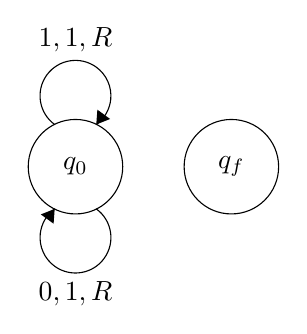
\begin{tikzpicture}[scale=0.2]
\tikzstyle{every node}+=[inner sep=0pt]
\draw [black] (36.1,-33.4) circle (3);
\draw (36.1,-33.4) node {$q_0$};
\draw [black] (46,-33.4) circle (3);
\draw (46,-33.4) node {$q_f$};
\draw [black] (37.423,-36.08) arc (54:-234:2.25);
\draw (36.1,-40.65) node [below] {$0,1,R$};
\fill [black] (34.78,-36.08) -- (33.9,-36.43) -- (34.71,-37.02);
\draw [black] (34.777,-30.72) arc (234:-54:2.25);
\draw (36.1,-26.15) node [above] {$1,1,R$};
\fill [black] (37.42,-30.72) -- (38.3,-30.37) -- (37.49,-29.78);
\end{tikzpicture}
\end{center}
\begin{align*}
	\Sigma &= \{0,1\} \\
	Q &= (q_0,q_f) \\
	\delta(q_0,0) &= (1,q_0,R) \\
	\delta(q_0,1) &= (1,q_0,R)
\end{align*}
\end{frame}

\begin{frame}\frametitle{Turing Machine --- Example}
	This machine will move left then right and so on\dots
	\begin{center}
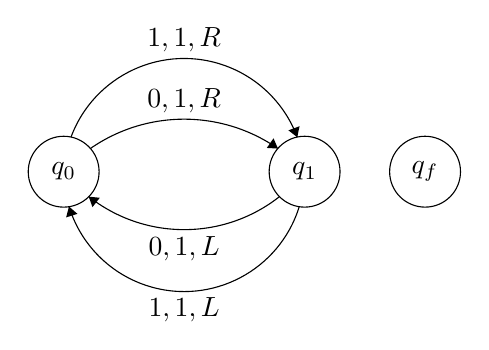
\begin{tikzpicture}[scale=0.15]
\tikzstyle{every node}+=[inner sep=0pt]
\draw [black] (22.8,-34) circle (3);
\draw (22.8,-34) node {$q_0$};
\draw [black] (43.2,-34) circle (3);
\draw (43.2,-34) node {$q_1$};
\draw [black] (53.4,-34) circle (3);
\draw (53.4,-34) node {$q_f$};
\draw [black] (23.42,-31.076) arc (159.6208:20.3792:10.22);
\fill [black] (42.58,-31.08) -- (42.77,-30.15) -- (41.83,-30.5);
\draw (33,-23.91) node [above] {$1,1,R$};
\draw [black] (25.062,-32.038) arc (124.76934:55.23066:13.92);
\fill [black] (40.94,-32.04) -- (40.57,-31.17) -- (40,-31.99);
\draw (33,-29.05) node [above] {$0,1,R$};
\draw [black] (42.747,-36.955) arc (-17.14503:-162.85497:10.2);
\fill [black] (23.25,-36.95) -- (23.01,-37.87) -- (23.97,-37.57);
\draw (33,-44.65) node [below] {$1,1,L$};
\draw [black] (41.076,-36.109) arc (-51.78538:-128.21462:13.055);
\fill [black] (24.92,-36.11) -- (25.24,-37) -- (25.86,-36.21);
\draw (33,-39.41) node [below] {$0,1,L$};
\end{tikzpicture}
\end{center}
\begin{align*}
	\Sigma &= \{0,1\} \\
	Q &= (q_0,q_1,q_f) \\
	\delta(q_0,0) &= (1,q_1,R) \\
	\delta(q_1,0) &= (1,q_0,L) \\
	\delta(q_0,1) &= (1,q_1,R) \\
	\delta(q_1,1) &= (1,q_0,L)
\end{align*}
\end{frame}

\begin{frame}\frametitle{Turing Machine --- Example}
The ADD Turing machine takes an input of two unary numbers separated by a $0$, $(1^l 0 1^m)$, then returns the sum of those two numbers, $(1^{l+m})$.
\begin{center}
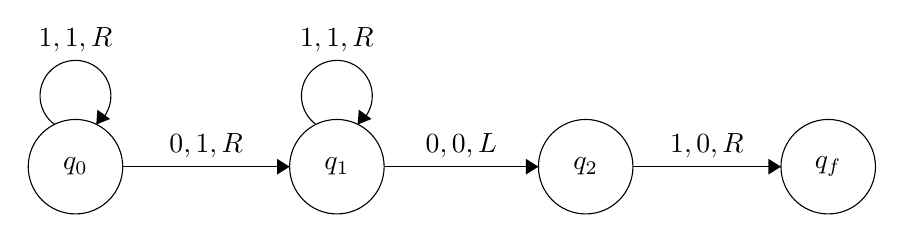
\begin{tikzpicture}[scale=0.2]
\tikzstyle{every node}+=[inner sep=0pt]
\draw [black] (13.4,-29.5) circle (3);
\draw (13.4,-29.5) node {$q_0$};
\draw [black] (30,-29.5) circle (3);
\draw (30,-29.5) node {$q_1$};
\draw [black] (45.8,-29.5) circle (3);
\draw (45.8,-29.5) node {$q_2$};
\draw [black] (61.2,-29.5) circle (3);
\draw (61.2,-29.5) node {$q_f$};
\draw [black] (12.077,-26.82) arc (234:-54:2.25);
\draw (13.4,-22.25) node [above] {$1,1,R$};
\fill [black] (14.72,-26.82) -- (15.6,-26.47) -- (14.79,-25.88);
\draw [black] (16.4,-29.5) -- (27,-29.5);
\fill [black] (27,-29.5) -- (26.2,-29) -- (26.2,-30);
\draw (21.7,-29) node [above] {$0,1,R$};
\draw [black] (28.677,-26.82) arc (234:-54:2.25);
\draw (30,-22.25) node [above] {$1,1,R$};
\fill [black] (31.32,-26.82) -- (32.2,-26.47) -- (31.39,-25.88);
\draw [black] (33,-29.5) -- (42.8,-29.5);
\fill [black] (42.8,-29.5) -- (42,-29) -- (42,-30);
\draw (37.9,-29) node [above] {$0,0,L$};
\draw [black] (48.8,-29.5) -- (58.2,-29.5);
\fill [black] (58.2,-29.5) -- (57.4,-29) -- (57.4,-30);
\draw (53.5,-29) node [above] {$1,0,R$};
\end{tikzpicture}
\end{center}
\begin{align*}
	\Sigma &= \{0,1\} \\
	Q &= (q_0,q_1,q_2,q_f) \\
	\delta(q_0,1) &= (1,q_0,R) \\
	\delta(q_0,0) &= (1,q_1,R) \\
	\delta(q_1,1) &= (1,q_1,R) \\
	\delta(q_1,0) &= (0,q_2,L) \\
	\delta(q_2,1) &= (0,q_f,R)
\end{align*}
\end{frame}

\begin{frame}\frametitle{(Deterministic / Probabilistic) Turing Machine}
\begin{figure}[H]
\includegraphics[width=.9\textwidth]{img/turing-machine-dp.pdf}	
\end{figure}
\end{frame}

\begin{frame}\frametitle{(Quantum) Turing Machine}
\begin{figure}[H]
\includegraphics[width=.9\textwidth]{img/turing-machine-q.pdf}	
\end{figure}
\end{frame}

\begin{frame}\frametitle{}
	\begin{thesis}[Church-Turing Thesis]
		\begin{center}
			\textcolor{green}{effective calculable} $=$ \textcolor{yellow}{recursive} $=$ Turing Computable\\
			$\scriptstyle ||$\\
			\textcolor{yellow}{representable in $\mathrm{Q}$} $=$ $\lambda$-definable\\
			$\scriptstyle ||$\\
			finite definable $=$ Herbrand-G\"odel computable\\
			$\scriptstyle ||$\\
			flowchart (or `while') computable\\
			$\scriptstyle ||$\\
			neural network with unbounded tape $=$ Conway's `game of life'\\
			$\scriptstyle ||$\\
			Post/Markov/McCarthy/Kolmogorov-Uspensky computable \ldots
		\end{center}
	\end{thesis}
	\begin{itemize}
		\item The behavior of any discrete physical system evolving according to local mechanical laws is computable?
		\item Any possible discrete physical process is computable?
		\item Any constructive function is computable?
		\item The mental functions can be simulated by machines?
	\end{itemize}
\end{frame}

\begin{frame}\frametitle{Church-Turing Thesis}
\begin{itemize}
	\item Church-Turing Thesis
\begin{quote}
	Every ``function which could be regarded as computable'' can be computed by a universal Turing machine.
\end{quote}
	\item Church-Turing-Deutsch Thesis
\begin{quote}
 	Every finite physical system can be simulated to any specified degree of accuracy by a universal Turing machine.
\end{quote}
\item Feasibility Thesis --- Classical / Quantum Version
\begin{quote}
 A probabilistic (quantum) Turing machine can efficiently simulate any realistic model of computation.
\end{quote}
\item Wolfram's Principle of Computational Equivalence
\begin{quote}
 	Almost all processes that are not obviously simple can be viewed as computations of equivalent sophistication.
\end{quote}
\item Wolfram's Principle of Computational Irreducibility
\begin{quote}
	Most of the time, the only way to see what a physical system (computer program) will do is to run it.
\end{quote}
\end{itemize}
\end{frame}

\begin{frame}\frametitle{Computational Irreducibility vs Free Will}
\begin{figure}[hbt]
\begin{center}
\includegraphics[width=\textwidth]{img/john.jpg}
\caption{To predict John's choice of breakfast by simulation. A universal computer in the safe (on the right) reproduces the outputs of another process, i.e.\ its observable actions (John preparing breakfast, on the left).}
\end{center}
\end{figure}
Libet: We are conscious of our free choices only after $300$ms our brain has made them.
\end{frame}

\begin{frame}\frametitle{}
\begin{figure}[H]
\includegraphics[width=\textwidth]{img/laplace-demon.jpeg}
\end{figure}
\end{frame}

\begin{frame}\frametitle{}
\begin{figure}[H]
\includegraphics[width=\textwidth]{img/laplace-chaos.jpeg}
\end{figure}
\end{frame}

\begin{frame}\frametitle{}
\begin{figure}[H]
\includegraphics[width=\textwidth]{img/laplace-entropy.jpeg}
\end{figure}
\end{frame}

%--------------------------%
\subsection{Rational Agents}
%--------------------------%

\begin{frame}\frametitle{Rationality $\ne$ Omniscience}
\begin{itemize}
	\item An omniscient agent percepts all relevant information, and knows the actual effects of its actions.
	\item A rational agent behaves according to its percepts and knowledge and attempts to maximize the expected performance.
\end{itemize}
Example: If I look both ways before crossing the street, and then as I cross I am hit by a meteorite, I can hardly be accused of lacking rationality.
\end{frame}

\begin{frame}\frametitle{The Ideal Rational Agent}
Rational behavior is dependent on
\begin{itemize}
	\item Performance measures (goals)
	\item Percept sequences
	\item Knowledge of the environment
	\item Possible actions
\end{itemize}
\begin{block}{Ideal rational agent}
For each possible percept sequence, a rational agent should select an action that is expected to maximize its performance measure, given the evidence provided by the percept sequence and whatever built-in knowledge the agent has.	
\end{block}
\centerline{Percept Sequence $\times$ World Knowledge $\to$ Action}
\end{frame}

\begin{frame}\frametitle{Agent Types}
\begin{itemize}
	\item \textbf{Table-driven agents:} use a percept sequence/action table in memory to find the next action.
	\item \textbf{Simple reflex agents:} based on condition-action rules, implemented with an appropriate production system, responds immediately to percepts.
	\item \textbf{Model-based agents:} have internal state, which is used to keep track of past states of the world.
	\item \textbf{Goal-based agents:} have goal information that describes desirable situations.
	\item \textbf{Utility-based agents:} base their decisions on classic axiomatic utility theory in order to act rationally.
	\item \textbf{Learning agents:} improve improves its performance w.r.t. a specific task with experience.
\end{itemize}
\end{frame}

\begin{frame}\frametitle{Agent?}
\begin{figure}[H]
	\includegraphics[width=.8\textwidth]{img/agent-box.pdf}
\end{figure}
\end{frame}

\begin{frame}\frametitle{Simple Reflex Agent}
\begin{figure}[H]
	\includegraphics[width=.8\textwidth]{img/agent-simple-reflex.pdf}
\end{figure}
Direct use of perceptions is often not possible due to the large space required to store them.
\end{frame}

\begin{frame}\frametitle{Model-based Reflex Agent}
\begin{figure}[H]
	\includegraphics[width=.8\textwidth]{img/agent-model-based-reflex.pdf}
\end{figure}
\end{frame}

\begin{frame}\frametitle{Model-based, Goal-based Agent}
\begin{figure}[H]
	\includegraphics[width=.8\textwidth]{img/agent-model-goal.pdf}
\end{figure}
\end{frame}

\begin{frame}\frametitle{Model-based, Utility-based Agent}
\begin{figure}[H]
	\includegraphics[width=.8\textwidth]{img/agent-model-utility.pdf}
\end{figure}
The agent can use utility function to weigh the importance of competing goals.
\end{frame}

\begin{frame}\frametitle{Learning Agent}
\vspace*{-1ex}
\begin{figure}[H]
	\includegraphics[width=.7\textwidth]{img/agent-learning.pdf}
\end{figure}
\begin{itemize}
	\item learning element (responsible for making improvements)
	\item performance element (processes percepts and chooses actions.)
	\item critic (evaluation of the agent's behavior)
	\item problem generator (suggests explorative actions that will lead to informative experiences)
\end{itemize}
\end{frame}

\begin{frame}\frametitle{Properties of Environments}
\begin{itemize}
	\item Accessible vs. inaccessible (fully observable vs. partially observable)\\
Are the relevant aspects of the environment accessible to the sensors?
	\item Deterministic vs. stochastic\\
Is the next state of the environment completely determined by the current state and the selected action?
	\item Episodic vs. sequential\\
Can the quality of an action be evaluated within an episode (perception $+$ action), or are future developments decisive for the evaluation of quality?
	\item Static vs. dynamic\\
Can the environment change while the agent is deliberating?
	\item Discrete vs. continuous\\
Is the environment discrete or continuous?
	\item Single agent vs. multi-agent\\
Which entities have to be regarded as agents? There are competitive and cooperative scenarios.
\end{itemize}
\end{frame}

\begin{frame}\frametitle{}
\begin{figure}[H]
\includegraphics[width=.5\textwidth]{img/crow.png}
\end{figure}
\begin{itemize}
	\item The crow can throw nuts from wires, so the cars underneath can break them.
	\item Then the crow waits for the traffic lights to turn green so he can eat his nuts in peace.
\end{itemize}
\end{frame}

%--------------------------%
\subsection{Search}
%--------------------------%

\begin{frame}\frametitle{Problem Solving by Searching}
\begin{itemize}
	\item Before an agent can start searching for solutions, it must formulate a goal and then use that goal to formulate a problem.
	\item A problem consists of five parts:
	\begin{enumerate}
	 	\item the state space
	 	\item initial situation
	 	\item actions
	 	\item goal test
	 	\item path costs
	 \end{enumerate}
	 A path from an initial state to a goal state is a solution.
	\item A general search algorithm can be used to solve any problem.\\
	Specific variants of the algorithm can use different search strategies.
	\item Search algorithms are judged on the basis of
	\begin{enumerate}
		\item completeness
		\item time complexity
		\item space complexity
		\item optimality
	\end{enumerate}
\end{itemize}
\end{frame}

\begin{frame}\frametitle{Criteria for Search Strategies}
\begin{description}
	\item[Completeness] Is the strategy guaranteed to find a solution when there is one?
	\item[Time Complexity] How long does it take to find a solution?
	\item[Space Complexity] How much memory does the search require?
	\item[Optimality] Does the strategy find the best solution (with the lowest path cost)?
\end{description}
\end{frame}

\begin{frame}\frametitle{}
\begin{figure}[H]
	\includegraphics[width=.8\textwidth]{img/search.pdf}
\end{figure}
\end{frame}

\begin{frame}\frametitle{Example --- Missionaries and Cannibals}
\begin{itemize}
	\item Three missionaries and three cannibals are on one side of a river.
	\item A boat is available that can hold at most two people.
	\item You must never leave a group of missionaries outnumbered by cannibals on the same bank.
	\item Find a strategy that brings everyone safely to the opposite bank.
\end{itemize}
\begin{description}
	\item[States] $(x,y,z)$ with $0\leq x,y\leq 3$ and $z\in\{0,1\}$, where $x,y$ and $z$ represent the number of missionaries, cannibals and boat currently on the original bank.
	\item[Initial State] $(3,3,1)$
	\item[Goal State] $(0,0,0)$
	\item[Path Costs] $1$ unit per crossing.
\end{description}
$(3,3,1)\to(3,1,0)\vee(2,2,0)\to(3,2,1)\to(3,0,0,)\to(3,1,1)\to(1,1,0)\to(2,2,1)\to(0,2,0)\to(0,3,1)\to(0,1,0)\to(0,2,1)\vee(1,1,1)\to(0,0,0)$
\end{frame}

\begin{frame}\frametitle{Problem Formulation}
\begin{block}{Question}
Given an $n\times n$ board from which two diagonally opposite corners have been removed (here $8\times 8$), can the board be covered with dominoes?
\end{block}
\begin{block}{Question --- Alternative Problem Formulation}
Can a board consisting of $n^2/2$ black and $n^2/2-2$ white squares be covered with dominoes s.t. each domino covers one black and one white square?
\end{block}
\begin{columns}
\column{.2\textwidth}
		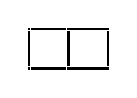
\begin{tikzpicture}[scale=0.5]
		\foreach \x[count=\x] in {0,1}{
			\node[fill,inner sep=0pt] (a\x) at (0,\x){};
		}
		
		\foreach \x[count=\x] in {0,1}{
			\node[fill,inner sep=0pt] (b\x) at (1,\x){};
		}
		
		\foreach \x[count=\x] in {0,1}{
			\node[fill,inner sep=0pt] (c\x) at (2,\x){};
		}
		
		\draw[thick] (a1) -- (b1);
		\draw[thick] (a1) -- (a2);
		\draw[thick] (a2) -- (b2);
		\draw[thick] (b1) -- (b2);
		\draw[thick] (c1) -- (c2);
		\draw[thick] (b1) -- (c1);
		\draw[thick] (b2) -- (c2);
		\end{tikzpicture}\qquad
		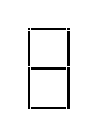
\begin{tikzpicture}[scale=0.5]
		\foreach \x[count=\x] in {0,1,2}{
			\node[fill,inner sep=0pt] (a\x) at (0,\x){};
		}
		
		\foreach \x[count=\x] in {0,1,2}{
			\node[fill,inner sep=0pt] (b\x) at (1,\x){};
		}
		
		\draw[thick] (a1) -- (b1);
		\draw[thick] (a1) -- (a2);
		\draw[thick] (a2) -- (a3);
		\draw[thick] (a3) -- (b3);
		\draw[thick] (b1) -- (b2);
		\draw[thick] (b2) -- (b3);
		\draw[thick] (a2) -- (b2);
		\end{tikzpicture}
\column{.37\textwidth}
		\includegraphics[width=\textwidth]{img/checkerboard.pdf}
\end{columns}
\end{frame}

\begin{frame}\frametitle{Search Strategies}
\begin{itemize}
	\item \textbf{Uninformed Search:} Rigid procedure with no knowledge of the cost of a given node to the goal.
	\item \textbf{Informed Search:} Knowledge of the worth of expanding a node $n$ is given in the form of an evaluation function $f(n)$.
\end{itemize}
\begin{block}{Uninformed or blind searches}
\begin{itemize}
	\item breadth-first search, depth-first search, lowest-cost-first search
	\item depth-limited search, iterative deepening search
	\item bi-directional search
\end{itemize}
\end{block}
\begin{block}{Informed Search Methods}
\begin{itemize}
	\item Best-First Search: expands the node with the best $f$-value first.
	\item $A^*$ and $\operatorname{IDA}^*$
	\item Local Search Methods: Hill Climbing / Gradient Decent.
	\item Genetic Algorithms
\end{itemize}
\end{block}
\end{frame}

\begin{frame}\frametitle{Breadth-first Search}
\begin{figure}[H]
	\includegraphics[width=\textwidth]{img/breadth1.pdf}	
\end{figure}	
\end{frame}

\begin{frame}\frametitle{Depth-first Search}
\begin{figure}[H]
	\includegraphics[width=\textwidth]{img/depth1.pdf}	
\end{figure}	
\end{frame}

\begin{frame}\frametitle{Best-First Search --- Greedy Search}
\begin{itemize}
	\item Idea: use an evaluation function for each node --- estimate of ``desirability'' --- expand most desirable unexpanded node
	\item $h(n)\coloneqq$ estimated path-costs from $n$ to the goal; $h(n)=0$ if $n$ is a goal.
	\item Greedy search: A best-first search using $h(n)$ as the evaluation function $f(n)=h(n)$.
	\item The evaluation function h in greedy searches is also called a \textcolor{red}{heuristic} function.
	\begin{itemize}
		\item Heuristics are fast but in certain situations incomplete methods for problem-solving.
		\item Heuristics are methods that improve the search in the average-case.
	\end{itemize}
\end{itemize}
\end{frame}

\begin{frame}\frametitle{$A^*$: combines greedy search with the lowest-cost-first search}
\begin{align*}
	g(n)&\coloneqq \mbox{actual cost so far from the initial state to reach } n\\
	h(n)&\coloneqq \mbox{estimated cost from $n$ to the nearest goal}\\
	f(n)&\coloneqq g(n)+h(n) \mbox{ estimated total cost of path through } n
\end{align*}
\begin{itemize}
	\item Idea: avoid expanding paths that are already expensive.
	\item $A^*$ uses an admissible heuristic $h(n)\leq h^*(n)$ to minimize the estimated path costs, where $h^*(n)$ is the actual cost of the optimal path from $n$
	\item $\operatorname{IDA}^*$: iterative-deepening $A^*$, where the $f$-costs are used to define the cutoff.
\end{itemize}
\end{frame}

\begin{frame}\frametitle{Heuristic Function Example}
\begin{figure}[H]
	\includegraphics[width=.8\textwidth]{img/tiles.pdf}
\end{figure}
\begin{align*}
	h_1&\coloneqq\mbox{the number of tiles in the wrong position}\\
	h_2&\coloneqq\mbox{the sum of the distances of the tiles from their goal positions}
\end{align*}
\end{frame}

\begin{frame}\frametitle{Local Search Methods}
\begin{itemize}
	\item In many problems, it is unimportant how the goal is reached, only the goal itself matters.
	\item If in addition a quality measure for states is given, local search can be used to find solutions.
	\item It operates using a single current node (rather than multiple paths).
	\item It requires little memory.
	\item Begin with a randomly-chosen configuration and improve on it step by step $\to$ \textbf{Hill Climbing(Gradient Ascent / Decent)}.\\
	``Like climbing Everest in thick fog with amnesia''
	\item \textbf{Simulated Annealing:} to escape local maxima, noise (``random walk'') is injected systematically: first a lot, then gradually less.
\end{itemize}
\begin{figure}[H]
	\includegraphics[width=.7\textwidth]{img/exploit-explore.pdf}
\end{figure}
\end{frame}

\begin{frame}\frametitle{Constraint Satisfaction Problems}
\begin{itemize}
	\item CSPs are a special kind of search problem, which consist of
	\begin{enumerate}
		\item a set of variables,
		\item a domain for each variable,
		\item a set of constraints.
	\end{enumerate}
	\item Example: Map-Coloring
	\begin{figure}[H]
	\includegraphics[width=.9\textwidth]{img/4color.png}
	\end{figure}
	\begin{enumerate}
		\item Variables: regions
		\item Values: $\{red,yellow,green,blue\}$
		\item Constraints: adjacent regions must have different colors
	\end{enumerate}
\end{itemize}
\end{frame}

\begin{frame}\frametitle{Heuristics}
\begin{itemize}
	\item Variable ordering: Which one to assign first?
	\begin{itemize}
		\item Most Constrained First: choose the variable with the fewest remaining legal values! reduces branching factor!
		\item Most Constraining Variable First: choose variable with the most constraints on remaining unassigned variables! reduces branching factor in the next steps.
		\item Least Constraining Value First: choose first a value that rules out the fewest values in the remaining unassigned variables
	\end{itemize}
	\item Value ordering: Which value to try first?
	\item Try to detect failures early on
	\item Try to exploit problem structure: tree structure
\end{itemize}
\end{frame}

%--------------------------%
\subsection{Logical Agent}
%--------------------------%

\begin{frame}\frametitle{Logic vs CS}
\[\dfrac{\text{Logic}}{\text{Computer Science}} \approx \dfrac{\text{Calculus}}{\text{Physics}}\]
	\begin{itemize}
		\item Computer Architecture.
		
		Logic gates and digital circuit design $\approx$ Propositional Logic
		\item Programming Languages.
		
		Semantics of programming languages via methods of logic\\
		LISP $\approx$ $\lambda$-calculus\\
		Prolog $\approx$ First Order Logic $+$ Recursion\\
		Typing $\approx$ Type Theory
		\item Theory of Computation and Computational Complexity.
		
		Models of computation (Turing machines, finite automata)\\
		Logic provides \emph{complete problems} for complexity classes.\\
		Logical characterizations of complexity classes\\
		Descriptive Complexity
	\end{itemize}
\end{frame}

\begin{frame}\frametitle{Logic vs CS}
	\begin{itemize}
		\item General Problem Solver (SAT solvers).
		\item Automated Theorem Proving.
		\item Knowledge representation via logic rules.
		\item Common sense reasoning via Non-monotonic Logic.
		\item Fuzzy Control vs Fuzzy Logic and Multi-valued Logic.
		\item Relational Databases.
		
		SQL $\approx$ First Order Logic $+$ Syntactic Sugar
		\item Software Engineering (Formal Specification and Verification).
		
		Extensive use of formal methods based on logic\\
		Temporal Logic, Dynamic Logic and Automata, Hoare Logic, Model Checking
		\item Multi-agent Systems.
		
		Epistemic Logic
		\item Semantic Web.
		
		Web Ontology Language (OWL) $\approx$ Description Logic
	\end{itemize}
\end{frame}

\begin{frame}\frametitle{Knowledge-based system architecture}
\begin{figure}[H]
	\includegraphics[width=\textwidth]{img/knowledge-based-agent.pdf}
\end{figure}
\end{frame}

\begin{frame}\frametitle{Offline and online decomposition of an agent}
\begin{figure}[H]
\includegraphics[width=\textwidth]{img/offline-online.pdf}
\end{figure}
\end{frame}

\begin{frame}\frametitle{}
\begin{figure}[H]
\includegraphics[width=.9\textwidth]{img/knowledge-based-architecture.pdf}
\end{figure}
\end{frame}

\begin{frame}\frametitle{Logical Agent: Knowledge-Based Agent}
\begin{figure}[H]
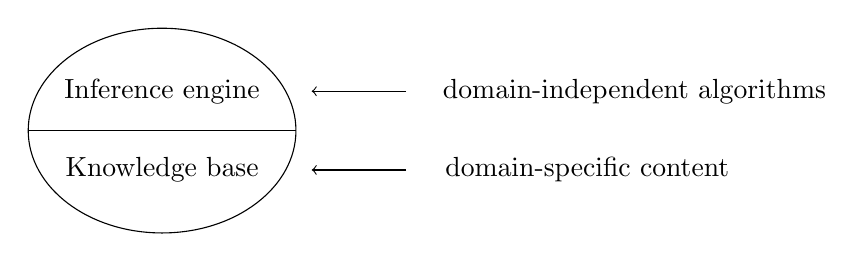
\begin{tikzpicture}
 \draw (-2.5, 0) ellipse (1.7 and 1.3);
 \draw (-4.2, 0) -- (-0.8, 0);
 \node at (-2.5, -0.5) {Knowledge base};
 \node at (-2.5, 0.5) {Inference engine};
 %\draw (1.5, 0) ellipse (0.9 and 1.5);
 %\draw (0.6, 0) -- (2.4, 0);
 \node at (2.9, -0.5) {domain-specific content};
 \node at (3.5, 0.5) {domain-independent algorithms};
 \draw [->] (0.6, 0.5) -- (-0.6, 0.5) node [pos=0.5, above] {};
 \draw [->] (0.6, -0.5) -- (-0.6, -0.5) node [pos=0.5, above] {};
\end{tikzpicture}
\end{figure}
A knowledge-based agent uses its knowledge base to
\begin{itemize}
	\item represent its background knowledge: states, actions, etc.
	\item incorporate new percepts
	\item update internal representations of the world
	\item deduce hidden properties of the world
	\item deduce appropriate actions
\end{itemize}
\end{frame}

\begin{frame}\frametitle{Entailment \& Deduction}
Before a system that is capable of learning, thinking, planning, explaining, \dots can be built, one must find a way to express knowledge.
\begin{itemize}
	\item syntax: formal structure of sentences
	\item semantics: truth of sentences wrt models
\end{itemize}
\[KB\vDash A\]
\[KB\vdash A\]
\begin{itemize}
	\item soundness: $KB\vdash A\implies KB\vDash A$
	\item completeness: $KB\vDash A\implies KB\vdash A$
\end{itemize}
Terminology: satisfiable, unsatisfiable, falsifiable, valid, logical equivalent
\end{frame}

\begin{frame}\frametitle{\small Model Checking \& Satisfiability Checking \& Validity Checking\footnote{\tiny \href{https://www.scottaaronson.com/papers/philos.pdf}{Aaronson: Why philosophers should care about computational complexity.}}}
	\begin{itemize}
		\item Given a model $\nu$ and a formula $A$. Is $\nu\vDash A$?\hfill ---\textcolor{yellow}{P}
		\item Given a formula $A$. Is there a model $\nu$ s.t. $\nu\vDash A$?\hfill ---\textcolor{yellow}{NP}
		\item Given a sentence $A$. Is $\vDash A$?
	\end{itemize}
\begin{minipage}{\textwidth}
	\begin{columns}
		\column{0.28\textwidth}
			\begin{figure}
				\includegraphics[width=\textwidth]{img/euler-bridge}\\
				\includegraphics[width=\textwidth]{img/eulerian-path}\caption{\tiny{\textit{Eulerian Circle(P)}}}
			\end{figure}
		\column{0.3\textwidth}\vspace{-0.3cm}
			\begin{figure}
				\includegraphics[width=0.7\textwidth]{img/hamiltonian-path}\vspace{-0.2cm}\caption{\tiny{\textit{Hamiltonian Circle(NPC)}}}\vspace{-0.2cm}
				\includegraphics[width=0.7\textwidth]{img/graph-coloring}\vspace{-0.3cm}\caption{\tiny{\textit{Graph Coloring(NPC)}}}
			\end{figure}
		\column{0.4\textwidth}\vspace{-0.5cm}
			\begin{center}
				\begin{figure}
					\includegraphics[width=\textwidth]{img/hanoi.pdf}
				\end{figure}
			\end{center}
	\end{columns}
\end{minipage}
\end{frame}

\begin{frame}\frametitle{Forward Reasoning, Backward Reasoning, Resolution}
\begin{enumerate}
	\item fire any rule whose premises are satisfied in the KB.
	\item add its conclusion to the KB, until query is found.
\end{enumerate}
\begin{itemize}
	\item Forward reasoning is \textbf{data-driven}, cf. automatic, unconscious processing.
	\begin{itemize}
		\item e.g. object recognition, routine decisions
	\end{itemize}
	May do lots of work that is irrelevant to the goal.
	\item Backward reasoning is \textbf{goal-driven}, appropriate for problem-solving.
	\begin{itemize}
		\item e.g. Where are my keys? How do I get into a PhD program?
	\end{itemize}
	\item Resolution Algorithm
	\[\infer{A\vee B}{A\vee C & B\vee\neg C}\]
	Proof by contradiction, i.e. show $KB,\neg A$ unsatisfiable.
\end{itemize}
\end{frame}

\begin{frame}\frametitle{}
\begin{figure}[H]
\includegraphics[width=.43\textwidth]{img/wumpus.pdf}
\end{figure}
\begin{itemize}
	\item \textbf{Frame problem:} find an elegant way to handle non-change
	\begin{itemize}
		\item representation: too many frame axioms
		\item inference: too many repeated ``copy-overs'' to keep track of state
	\end{itemize}
	\item \textbf{Qualification problem:} can never finish listing all required preconditions of actions, and possible conditional outcomes of actions
	\begin{itemize}
		\item what if gold is slippery or nailed down or \dots
	\end{itemize}
	\item \textbf{Ramification problem:} real actions have many secondary consequences.
	\begin{itemize}
		\item what about the dust on the gold, wear and tear on gloves \dots
	\end{itemize}
\end{itemize}
\end{frame}

\begin{frame}\frametitle{Frame Problem}
\begin{itemize}
	\item How to represent the effects of an action in logic without having to represent explicitly a large number of intuitively obvious non-effects.
	\item Is it possible to limit the scope of the reasoning required to derive the consequences of an action?
	\item How to limit the beliefs that have to be updated in response to an action.
\end{itemize}
\end{frame}

\begin{frame}\frametitle{Wittgenstein 1889-1951 Tractatus Logico-Philosophicus}
\begin{figure}[H]
\includegraphics[width=.25\textwidth]{img/wittgenstein.jpg}
\end{figure}
\begin{enumerate}
	\item The world is all that is the case.
	\item What is the case, the fact, is the existence of states of affairs.
	\item A logical picture of facts is a thought.
	\item A thought is a proposition with a sense.
	\item A proposition is a truth-function of elementary propositions.\\
	(An elementary proposition is a truth-function of itself.)
	\item The general form of a truth function is: $[\overline{p},\overline{\xi},N(\overline{\xi})]$.\\
	This is the general form of a proposition.
	\item Whereof one cannot speak, thereof one must be silent.
\end{enumerate}
\end{frame}

\begin{frame}\frametitle{Language --- Mind --- World}
\begin{itemize}
	\item What is the meaning of `meaning'? (symbol grounding problem)
	\item How do words relate to objects?
	\item How do words relate to thought?
	\item What makes a sentence true/false?
\end{itemize}
\begin{table}
\begin{tabu}{ccc}
proper name & predicate & sentence \\
$\downarrow$ & $\downarrow$ & $\downarrow$ \\
sense of the proper name & sense of the predicate & thought\\
$\downarrow$ & $\downarrow$ & $\downarrow$ \\
reference/object & concept & truth-value \\
 & $\downarrow$ & \\
 & $\begin{array}{c}
 	\mbox{object that falls}\\
 	\mbox{under the concept}
 \end{array}$ &
\end{tabu}\caption{Frege: sense \& reference}
\end{table}
The intension of an expression is a function from each possible world to the extension of the expression.
\centerline{Wittgenstein: The limits of my language means the limits of my world.}
\end{frame}

\begin{frame}\frametitle{What is the meaning of `meaning'?}
\[
\begin{tikzcd}
\text{flying horse} \arrow[r] \& 
\raisebox{-2cm}{\includegraphics[width=.3\textwidth]{img/flying-horse.jpeg}}
\end{tikzcd}
\]
\begin{itemize}
	\item The morning star is the evening star.
	\item Sherlock Holmes is a detective.
	\item The flying horse is not a horse.
	\item The present King of France is bald.
	\item The round square is round.
	\item The golden mountain does not exist.
\end{itemize}
\end{frame}

\begin{frame}\frametitle{Frege 1848-1925 (+Peirce)}
	\begin{columns}
		\column{0.77\textwidth}
			\begin{itemize}
				\item \emph{Begriffsschrift, a formal language of pure thought modelled upon that of arithmetic.}
				\item Predicate Logic. (Relation \& Quantification)\\
				\textcolor{yellow}{(Every boy loves some girl.)}
				\[\dfrac{\text{subject}}{\text{predicate}} \approx \dfrac{\text{argument}}{\text{function}}\]
				\item Philosophy of Language.\\
				\textcolor{yellow}{The evening star is the morning star. (venus)}
			\end{itemize}
		\column{0.2\textwidth}
			\begin{figure}
				\includegraphics[width=\textwidth,angle=0,origin=c]{img/frege-painting}
			\end{figure}
	\end{columns}
	\centerline{\textcolor{red}{\fbox{Logicism}} Mathematics $\rightsquigarrow$ Logic.\footnote{\tiny Frege: The Foundations of Arithmetic.}}
\end{frame}

\begin{frame}\frametitle{Reducing First Order Inference to Propositional Inference}
\begin{itemize}
	\item Universal Instantiation
	\[\infer[\text{where $t$ is a ground term}]{A[t/x]}{\forall xA}\]
	\begin{itemize}
		\item can be applied several times to add new sentences
		\item the new KB is logically equivalent to the old
	\end{itemize}
	\item Existential Instantiation
	\[\infer[\text{where $a$ is a new constant}]{A(a)}{\exists xA}\]
	\begin{itemize}
		\item can be applied once to replace the existential sentence
		\item the new KB is not equivalent to the old
		\item but is satisfiable iff the old KB was satisfiable
	\end{itemize}
\end{itemize}
\end{frame}

\begin{frame}\frametitle{Reducing First Order Inference to Propositional Inference}
\begin{itemize}
	\item Claim: a sentence is entailed by the new KB iff it is entailed by the original KB
	\item Claim: every FOL KB can be propositionalized so as to preserve entailment
\end{itemize}
\begin{theorem}[Herbrand's Theorem]
If a sentence $A$ is entailed by an FOL KB, it is entailed by a finite subset of the propositional KB.
\end{theorem}
\begin{itemize}
	\item Idea: propositionalize KB and query, apply resolution, return result
	\item[] \hspace{-1em}\textcolor{red}{for} \textcolor{green}{$n=0$ to $\infty$} \textcolor{red}{do}\\
	\textcolor{green}{create a propositional KB by instantiating with depth-$n$ terms see if $A$ is entailed by this KB}
	\item Problem: works if $A$ is entailed, loops if $A$ is not entailed
	\item Theorem (Turing, Church): entailment in FOL is semidecidable.
\end{itemize}
\end{frame}

%--------------------------%
\subsection{Knowledge Representation}
%--------------------------%

\begin{frame}\frametitle{}
\begin{quote}
Where is the Life we have lost in living?\\
Where is the wisdom we have lost in knowledge?\\
Where is the knowledge we have lost in information?\par
\hfill --- \textsl{T. S. Eliot}
\end{quote}
\begin{figure}[H]
\includegraphics[height=.27\textwidth]{img/garbage-brain.jpg}
\includegraphics[height=.27\textwidth]{img/garbage-in-out.png}
\end{figure}
\begin{itemize}
	\item We are drowning in information and starving for knowledge.
	\item A wealth of information creates a poverty of attention.
\end{itemize}
\end{frame}

\begin{frame}\frametitle{}
\begin{figure}[H]
\includegraphics[width=.85\textwidth]{img/dikw0.png}
\includegraphics[width=.85\textwidth]{img/dikw1.png}
\end{figure}
\end{frame}

\begin{frame}\frametitle{Knowledge}
\begin{itemize}
	\item Goal: common sense reasoning
	\item Need to represent knowledge about the world
	\begin{itemize}
		\item Representational adequacy: ability to represent the required knowledge
		\item Inferential adequacy: ability to manipulate knowledge $\implies$ produce new knowledge
		\item Inferential efficiency: ability to respond with limited resources (time, storage)
		\item Acquisitional efficiency: ability to acquire new knowledge, ideally, automatically
	\end{itemize}
	\item Types of knowledge
	\begin{itemize}
		\item categories \& objects $\to$ ontologies
		\item frames
		\item events: fluents, time interval, scripts
		\item procedures
		\item relations
		\item mental states
		\item meta knowledge
	\end{itemize}
	\item Know that, Know whether, Know what, Know how, Know why, Know who \dots
\end{itemize}
\end{frame}

\begin{frame}\frametitle{Conceptualization \& Ontology}
\begin{itemize}
	\item A knowledge representation is a set of ontological commitments.
	\item A \textcolor{red}{conceptualization} is a map from the problem domain into the representation. A conceptualization specifies:
	\begin{itemize}
		\item What sorts of objects are being modeled
		\item The vocabulary for specifying objects, relations and properties
		\item The meaning or intention of the vocabulary
	\end{itemize}
	\item An \textcolor{red}{ontology} is a specification of a conceptualization. An ontology specifies the meanings of the symbols in an information system.
	\begin{enumerate}
		\item Decide what to talk about
		\item Decide on a vocabulary of predicates, functions and constants
		\item Encode general knowledge about the domain
		\item Encode a description of the specific problem instance
		\item Pose queries to the inference procedure and get answers
	\end{enumerate}
\end{itemize}
\end{frame}

\begin{frame}\frametitle{A Structured Semantic Network}
\begin{figure}[H]
\includegraphics[width=.9\textwidth]{img/semantic-network.pdf}	
\end{figure}
\end{frame}

\begin{frame}\frametitle{Semantic Web \& Ontology}
\begin{itemize}
	\item The same symbol means the same thing across the various web sites that obey the ontology.
	\item If someone wants to refer to some other object or relation, they publish the terminology with its intended interpretation.\\
	Others adopt the new terminology by using it and referring to its source. In this way, ontologies grow.
	\item Separately developed ontologies can have mappings between them published.
\end{itemize}
However
\begin{itemize}
	\item How one divides the world can depend on the application. Different ontologies describe the world in different ways.
	\item People can fundamentally disagree about the appropriate structure.
	\item Different knowledge bases can use different ontologies.
	\item To allow KBs based on different ontologies to inter-operate, there must be mapping between different ontologies.
	\item The computer doesn't understand the meaning of the symbols. The formalism can constrain the meaning, but can't define it.
\end{itemize}
\end{frame}

\begin{frame}\frametitle{A brief history of ontology}
\begin{description}
	\item[Descartes] Central role of mind.\\
	Dualism of mind and matter.
	\item[Kant] Reality is unknowable.\\
	Metaphysics is impossible.\\
	We can only know the quasi-fictional domains which we ourselves create.\\
	The mind imposes its categories on the data of experience.
	\item[Russell] Logic as mirror of reality.
	\item[Wittgenstein] Centrality of language and of language games.
	\item[Quine] Ontological commitment (study not: what there is, but: what sciences believe there is when logically formalized)
	\item[Hayes] Ontology to build Robots.\\
	Ontological commitment $=$ study what people believe there is when logically formalized.
\end{description}
\end{frame}

\begin{frame}\frametitle{Classical Empiricism}
	\begin{figure}
		\includegraphics[width=\textwidth]{img/classical-empiricism.pdf}\caption{Locke, Berkeley, Hume: The only source of knowledge of the external world is experience.}
	\end{figure}
	\begin{itemize}
		\item How is knowledge of the external world possible?
		\item How is knowledge of the future based only on past experience possible?
	\end{itemize}
\end{frame}

\begin{frame}\frametitle{Hume 1711-1776}
\begin{columns}
\column{.4\textwidth}
\begin{figure}[H]
\includegraphics[width=\textwidth]{img/hume.jpg}	
\end{figure}
\column{.5\textwidth}
\begin{itemize}
	\item ``Reason and rational judements are merely habitual associations of distinct sensations or experiences.''
	\item Problem of Induction
	\item Assiciation $\centernot\to$ Causation
	\item Belief $\centernot\to$ Knowledge
	\item Is $\centernot\to$ Ought to Be
	\item \textcolor{red}{\Large No-Free-Lunch!}
	\item Connectionism
	\item Analogy
	\item Counterfactual Causation
\end{itemize}
\end{columns}
\end{frame}

\begin{frame}\frametitle{Hume vs Connectionism}
\[
\begin{tikzcd}
\text{data} \arrow[r,"sensor"] \& \text{impression} \arrow[rrr,"neural-network"] \&\&\& \text{idea} \arrow[rr,"imagination"] \&\& \text{complex ideas}
\end{tikzcd}
\]
\begin{itemize}
	\item There are three different principles of association: resemblance, spatial and temporal contiguity, and causation, which purport to capture the regularities by which the imagination recombines simple ideas into complex ideas.
	\item The memory, senses, and understanding are founded on the imagination, or the vivacity of our ideas.
\end{itemize}
Traditional associationist architectures represent knowledge by simple connection weights. (e.g., between the nodes of a neural network)\\
Bayesian associative models represent knowledge as probability distributions consisting of graded degrees of belief.
\end{frame}

\begin{frame}\frametitle{Rationalism}
	\begin{figure}
		\includegraphics[width=\textwidth]{img/rationalism.pdf}\caption{Descartes: There can be certain knowledge based on pure reason alone.}
	\end{figure}
	a priori knowledge $=$ certain knowledge independent of experience.
\end{frame}

\begin{frame}\frametitle{Kant 1724-1804}
\begin{table}
\abovetabulinesep=1mm
\belowtabulinesep=1mm
	\begin{tabu}{c|c|c}
		\hline
		 & \texttt{a priori} & \texttt{a posteriori} \\
		\hline
		analytic & $\checkmark$ & $\times$ \\
		synthetic & \textcolor{red}{?} & $\checkmark$ \\
		\hline
	\end{tabu}
\end{table}
\begin{columns}
\column{.35\textwidth}
	\begin{figure}
		\includegraphics[width=\textwidth]{img/kant.jpg}
	\end{figure}
\column{.42\textwidth}
	Synthetic a priori statement $=$ truth is established by reason alone (a priori) and contains factual content (synthetic).
\end{columns}
\end{frame}

\begin{frame}\frametitle{Kant}
	\begin{figure}
		\includegraphics[width=\textwidth]{img/kant-filter.pdf}\caption{Kant: All structure and order (causal, temporal, spatial, etc) is imposed on raw data by filters (``forms'') already present in the mind.}
	\end{figure}
\end{frame}

\begin{frame}\frametitle{Empiricism / Rationalism vs Connectionism / Symbolism}
\[
\begin{tikzcd}
\& \text{\textcolor{green}{data}} \arrow[d] \\
\text{prior knowledge} \arrow[r] \& \fbox{\textcolor{red}{learning}} \arrow[r] \& \text{knowledge/belief?} \arrow[ll,dashed,bend left]
\end{tikzcd}
\]	
\end{frame}

\begin{frame}\frametitle{Logical Positivism}
\begin{itemize}
	\item Analytic-Synthetic Distinction
	\begin{itemize}
		\item analytic sentence $=$ a sentence that is true/false in virtue of its meaning.
		\item synthetic sentence $=$ a sentence that is true/false in virtue of its meaning and how the world actually is.
	\end{itemize}
	\item Verifiability Theory of Meaning: The meaning of a sentence consists in its method of verification.
	\begin{itemize}
		\item It's too weak! e.g. ``All metals expand when heated and the Absolute Spirit is perfect'' is verifiable.
		\item It's too strong! e.g. ``Superstrings exist'' is not verifiable.
	\end{itemize}
	\item Observational \& Theoretical Languages
	\item The Role of Logic: analyze the language of science in terms of logic (Deductive \& Inductive).
\end{itemize}
\textbf{Problems:}
\begin{itemize}
	\item Hypotheses cannot be tested in isolation (Duhem-Quine Thesis).
	\item Nothing is immune to revision, not even logic (analytic sentences).
	\begin{itemize}
		\item[---] Move from classical to quantum physics requires analogous move from classical to quantum logic!
	\end{itemize}
\end{itemize}
\end{frame}

\begin{frame}\frametitle{Popper --- Falsificationism}
\begin{itemize}
	\item A theory is falsifiable if it is contradicted by an observation that is expressible in the language of the theory.
	\item However, it is models of theories, not the theories themselves, that are tested by experiments.
	\item In general, it is possible to falsify a parametric family of models, but impossible to falsify the class of all models of the theory, for it is too large.
\end{itemize}
\end{frame}

\begin{frame}\frametitle{From Logical Positivism to Logical Empiricism}
\begin{itemize}
	\item Verifiability Theory of Meaning: The meaning of a sentence consists in its method of verification.
	\item Holistic Empiricist Theory of Meaning: Theoretical claims about unobservable phenomena gain meaning from their place in the structure of a given theory.
\end{itemize}
\begin{figure}[H]
\includegraphics[width=.95\textwidth]{img/logical-empiricism.pdf}	
\end{figure}
\end{frame}

\begin{frame}\frametitle{Wittgenstein: Philosophical Investigations}
\begin{quote}
``I shall not today attempt further to define `pornography'; and perhaps I could never succeed in intelligibly doing so. But I know it when I see it.''\par
\hfill --- \textsl{Potter Stewart}	
\end{quote}
\begin{itemize}
	\item We cannot define words.
	\item Language does not describe facts, it is used to communicate.
	\item The meaning of a word is its use in the language.
	\item The various uses of words can be best understood as family resemblance.
	\begin{itemize}
		\item use $A$ is similar to use $B$, because they share trait $X$
		\item use $B$ is similar to use $C$, because they share trait $Y$
	\end{itemize}
	\item If a word is used in a new context, we draw on the various uses in other contexts.
\end{itemize}
\end{frame}

\begin{frame}\frametitle{Wittgenstein: Philosophical Investigations}
\begin{itemize}
	\item How are chairs identified?
	\item chair $= 4$ legs, back, seat, used for sitting, \dots
	\begin{figure}
	\includegraphics[height=.2\textwidth]{img/chair1.jpg}
	\includegraphics[height=.2\textwidth]{img/chair2.jpg}
	\includegraphics[height=.2\textwidth]{img/chair3.jpg}
	\includegraphics[height=.2\textwidth]{img/chair4.jpg}
	\end{figure}
	\item All chairs share a ``family resemblance'' in appropriate contexts of use.
	\item This family resemblance can't be formally encoded in a rule/definition.
	\item form of life $=$ basic set of practices, behaviors, principles (\textcolor{yellow}{No external justification.})
	\item language game $=$ pattern of linguistic habits associated with a form of life.
	\item Language does not represent; rather, it is used by communities to communicate.
	\item Terms do not gain meaning by what they represent; rather, they gain meaning by how they are used.
\end{itemize}
\end{frame}

\begin{frame}\frametitle{Wittgenstein --- On Certainty}
\begin{figure}[H]
\includegraphics[width=.35\textwidth]{img/river-bed.jpeg}
\end{figure}
\begin{itemize}
	\item The propositions describing this world-picture might be part of a kind of mythology. And their role is like that of rules of a game; and the game can be learned purely practically, without learning any explicit rules.
	\item The mythology may change back into a state of flux, river-bed of thoughts may shift. But I distinguish between movement of the waters on the river-bed and the shift of the bed itself; though there is not a sharp division of the one from other.
	\item And the bank of that river consists partly of hard rock, subject to no alteration or only to an imperceptible one, partly of sand, which now in one place now in another gets washed away, or deposited.
\end{itemize}
\end{frame}

\begin{frame}\frametitle{Quine 1908-2000 ``web of belief''}
\begin{figure}[H]
\includegraphics[height=.37\textwidth]{img/quine.jpg}
\includegraphics[height=.37\textwidth]{img/gavagai.jpeg}
\end{figure}
\begin{itemize}
	\item Scientific claims, common beliefs and opinions, are all interconnected in a single unified belief system.
	\item Changes in any part of the system can be accomodated by revision elsewhere.\\
	(It confronts experience as a whole.)\\
	\item Indeterminacy of translation
\end{itemize}
\end{frame}

\begin{frame}\frametitle{}
\begin{itemize}
	\item Holistic Theory of Meaning: A scientific term gets its meaning from the theory it appears in.
	\item There is no single set of standards entitled to govern the justification of beliefs.
	\item Justification of a belief system is internal to that system, not external.
	\item Scientific theories (facts) are social constructs.
\end{itemize}
\begin{block}{What does ``social construct'' mean?}
To construct $X$ in the social world requires:
\begin{itemize}
	\item Knowledge of $X$ encourages behaviors that increase or reduce other people's tendency to act as though $X$ does or does not exist.
	\item There is reasonably common knowledge of $X$
	\item There is transmission of knowledge of $X$.
\end{itemize}
\end{block}
\end{frame}

\begin{frame}\frametitle{Philosophy of Language}
\begin{itemize}
	\item ``Classical'' view (pre-1953): language consists of sentences that are true/false
	\item ``Modern'' view (post-1953): language is a form of action
\end{itemize}
Wittgenstein (1953), Philosophical Investigations\\
Austin (1962), How to Do Things with Words\\
Searle (1969), Speech Acts
\[
\fbox{
\begin{tikzcd}
\text{\small situation}\\
\textit{\textcolor{green}{Speaker}} \arrow[r] \& \textit{\textcolor{red}{Utterance}} \arrow[r] \& \textit{\textcolor{green}{Hearer}}
\end{tikzcd}
}
\]
\begin{itemize}
	\item Speech acts achieve the speaker's goals.
	\item Speech act planning requires knowledge of\\
	--- Situation\\
	--- Semantic and syntactic conventions\\
	--- Hearer's goals, knowledge base, and rationality
\end{itemize}
\end{frame}

\begin{frame}\frametitle{Stages in Communication}
\begin{table}
\begin{tabu}{ll}
\textbf{Intention} & $S$ wants to inform $H$ that $P$\\
\textbf{Generation} & $S$ selects words $W$ to express $P$ in context $C$\\
\textbf{Synthesis} & $S$ utters words $W$
\end{tabu}
\end{table}
\begin{table}
\begin{tabu}{ll}
\textbf{Perception} & $H$ perceives $W'$ in context $C'$\\
\textbf{Analysis} & $H$ infers possible meanings $P_1,\dots,P_n$\\
\textbf{Disambiguation} & $H$ infers intended meaning $P_i$\\
\textbf{Incorporation} & $H$ incorporates $P_i$ into $\operatorname{KB}$
\end{tabu}
\end{table}
Engaging in complex language behavior requires various kinds of knowledge of language
\begin{itemize}
	\item \textcolor{green}{Linguistic knowledge:} Phonetics, phonology, Morphology, Syntax, Semantics, Pragmatics, Discourse
	\item \textcolor{green}{World knowledge:} common knowledge, commonsense knowledge
\end{itemize}
\end{frame}

\begin{frame}\frametitle{NLP --- Word Embedding}
\begin{itemize}
\item A word embedding $W$ is a function
\[W:\mbox{words}\to\mathbb{R}^n\]
which maps words of some language to a high-dimensional vector space.
\item Mapping function $W$ should be realized by a neural network such that:
\begin{itemize}
	\item representations in $\mathbb{R}^n$ of related words have a short distance
	\item representations in $\mathbb{R}^n$ of unrelated words have a large distance
\end{itemize}
\item A word embedding function $W$ can be trained using different tasks, that require the network to discriminate related from unrelated words.
\begin{itemize}
	\item Example: Train the combination of embedding function $W$ and classification module $R$:
\begin{align*}
	R(W(cat),W(sat),W(on),W(the),W(mat))&=1\\
	R(W(cat),W(sat),W(song),W(the),W(mat))&=0
\end{align*}
\end{itemize}
\end{itemize}
\end{frame}

\begin{frame}\frametitle{}
\begin{figure}[H]
	\includegraphics[width=.9\textwidth]{img/word2vec.png}
\end{figure}
\centerline{King $-$ Man $+$ Woman $\approx$ Queen}
\textbf{Remark:} ``King $-$ Man $+$ Woman'' doesn't exactly equal ``Queen'', but ``Queen'' is the closest word to it.
\end{frame}

\begin{frame}\frametitle{What is the meaning of `meaning'?}
\begin{itemize}
	\item Distributed Representations of words as word vectors.
	\item Why are they vectors?
	\begin{itemize}
		\item Similarity-is-Proximity: two similar things are conceptualized as being close to or near each other.
		\item Entities-are-Locations: in order for two things to be close to each other, they need to have a spatial location.
		\item Geometric Metaphor of meaning: Meanings are points in space, and the proximity among their locations is a measure of their semantic similarity.
		\[\displaystyle{\text{similarity}}=\cos\theta = \frac{\mathbf{A} \cdot \mathbf{B}}{\|\mathbf{A}\| \|\mathbf{B}\|} = \frac{\sum\limits_{i=1}^n A_iB_i}{\sqrt{\sum\limits_{i=1}^n{A_i^2}} \sqrt{\sum\limits_{i=1}^n{B_i^2}}}\]
		\item Words with similar distributional properties have similar meanings.
	\end{itemize}
\end{itemize}
\begin{quote}
``You shall know a word by the company it keeps.''\par
\hfill --- \textsl{Firth}
\end{quote}
\end{frame}

\begin{frame}\frametitle{System $1$ vs System $2$ --- Thinking, Fast and Slow --- Kahneman}
\begin{block}{System $1$}
\begin{itemize}
	\item Intuitive, fast, unconscious, $1$-step parallel, non-linguistic, habitual
	\item Implicit knowledge
\end{itemize}	
\end{block}
\begin{block}{System $2$}
\begin{itemize}
	\item Slow, logical, sequential, conscious, linguistic, algorithmic, planning, reasoning 
	\item Explicit knowledge
	\item Manipulates high-level / semantic concepts, which can be recombined combinatorially
\end{itemize}	
\end{block}
\begin{itemize}
	\item High-level representations $\leftrightarrow$ language
	\item High-level concepts: meaning anchored in low-level perception and action $\to$ tie system $1$ \& $2$
	\item Grounded high-level concepts $\to$ better language understanding
\end{itemize}
\end{frame}

\begin{frame}\frametitle{System $1$ vs System $2$ --- Thinking, Fast and Slow --- Kahneman}
\vspace*{-3ex}
\begin{columns}
\column{.29\textwidth}
\begin{figure}[H]
\includegraphics[width=\textwidth]{img/system1.jpg}
\end{figure}
\column{.47\textwidth}
\[
\begin{tikzcd}[column sep=huge, cells={nodes={draw=gray}}]
\mbox{System $1$}\atop\text{Intuitive} \arrow[r, yshift=1ex, bend left] \& \mbox{System $2$}\atop\text{Analytic} \arrow[l, yshift=-1ex, bend left]
\end{tikzcd}
\]
\column{.29\textwidth}
\begin{figure}[H]
\includegraphics[width=\textwidth]{img/system2.jpg}
\end{figure}
\end{columns}
\vspace*{-1ex}
\begin{figure}[H]
\includegraphics[height=.21\textwidth]{img/system12.jpeg}
\includegraphics[height=.21\textwidth]{img/kahneman1.jpeg}
\end{figure}
\vspace*{-2ex}
\begin{itemize}
	\item System $1$\\
	--- extract entities to build the cognitive graph\\
	--- generate semantic vectors for each node
	\item System $2$\\
	--- do reasoning based on semantic vectors and graph\\
	--- feed clues to System 1 to extract next-hop entities
\end{itemize}
\end{frame}

\begin{frame}\frametitle{Implicit vs Verbalizable Knowledge}
\begin{itemize}
	\item Most knowledge in our brain is implicit and not verbalizable (hence the explainability challenge, even for humans)
	\item Some of our knowledge is verbalizable and we can reason and plan explicitly with it
	\item The concepts manipulated in this way are those we can name with language
\end{itemize}
\begin{figure}[H]
\includegraphics[width=.4\textwidth]{img/iceberg.png}	
\end{figure}
\end{frame}

\begin{frame}\frametitle{From Perception to Modelling the World at the Semantic-Level}
\begin{itemize}
	\item What are the right representations? Causal variables explaining the data
	\item How to discover them (as a function of observed data)?
	\item How to discover their causal relationship, the causal graph?
	\item How are actions corresponding to causal interventions?
	\item How is raw sensory data mapped to high-level causal variables and how do high-level causal variables turn into low-level actions and partial observations?
\end{itemize}	
\end{frame}

\begin{frame}\frametitle{Abstract Representation of the Physical World}
\[\resizebox{1.03\textwidth}{!}{
	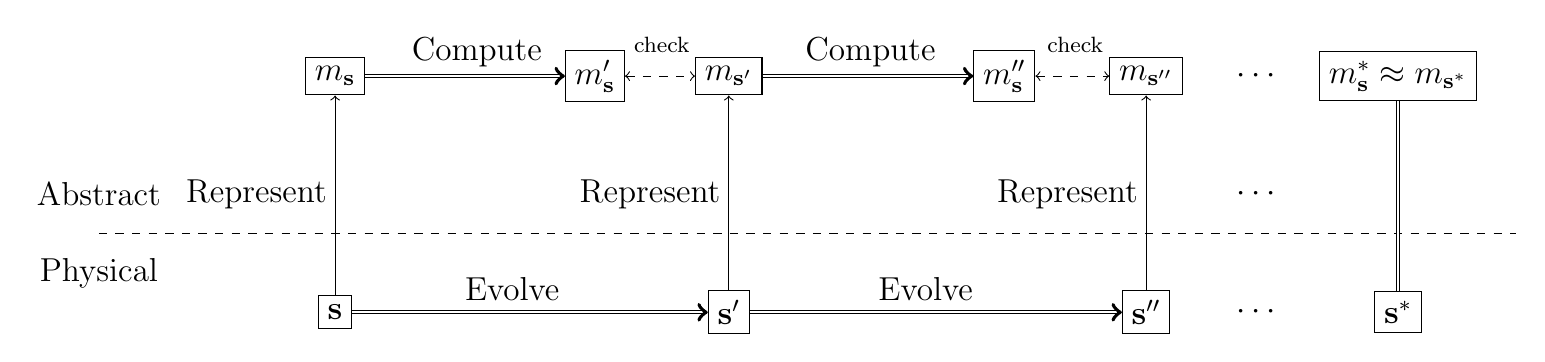
\begin{tikzpicture}[font=\large]
	\draw[style=dashed] (0,0) -- (18,0);
	\draw (0,0.5) node {Abstract};
	\draw (0,-0.5) node {Physical};
	%fig a
	\node[draw] (p) at (3,-1) {$\mathbf{s}$};
	\node[draw] (mp) at (3,2) {$m_{\mathbf{s}}$};
	\draw[->] (p) -- (mp);
	%\draw (3.4,0.5) node {$\mathcal{R}_T$};
	\draw (2,0.5) node {\text{Represent}};
	%fig b
	\node[draw] (mprp) at (6.3,2) {$m'_{\mathbf{s}}$};
	\draw[->,double] (mp) -- (mprp);
	\draw (4.8,2.3) node {Compute};
	%\draw (4.8,1.7) node {Compute};
	%fig c
	\node[draw] (ppr) at (8,-1) {$\mathbf{s}'$};
	\draw[->,double] (p) -- (ppr);
	\draw (5.25,-.7) node {\text{Evolve}};
	%fig d
	\node[draw] (mppr) at (8,2) {$m_{\mathbf{s}'}$};
	\draw[->] (ppr) -- (mppr);
	%\draw (8.4,0.5) node {$\mathcal{R}_T$};
	\draw (7,0.5) node {Represent};
	%epsilon
	\draw[<->,style=dashed] (mprp) to (mppr);
	\draw (7.15,2.4) node {\footnotesize{check}};
	%fig b'
	\node[draw] (mpprp) at (11.5,2) {$m_{\mathbf{s}}''$};
	\draw[->,double] (mppr) -- (mpprp);
	\draw (9.8,2.3) node {Compute};
	%\draw (9.8,1.7) node {Compute};
	%fig c'
	\node[draw] (pppr) at (13.3,-1) {$\mathbf{s}''$};
	\draw[->,double] (ppr) -- (pppr);
	\draw (10.5,-.7) node {\text{Evolve}};
	%fig d
	\node[draw] (mpppr) at (13.3,2) {$m_{\mathbf{s}''}$};
	\draw[->] (pppr) -- (mpppr);
	%\draw (13.7,0.5) node {$\mathcal{R}_T$};
	\draw (12.3,0.5) node {\text{Represent}};
	%epsilon
	\draw[<->,style=dashed] (mpprp) to (mpppr);
	\draw (12.4,2.4) node {\footnotesize{check}};
	\draw (14.7,2) node {$\cdots$};
	\draw (14.7,0.5) node {$\cdots$};
	\draw (14.7,-1) node {$\cdots$};
	\node[draw] (minf) at (16.5,2){$m_{\mathbf{s}}^* \approx m_{\mathbf{s}^*}$};
	\node[draw] (infr) at (16.5,-1){$\mathbf{s}^*$};
	\draw[-,double] (minf) to (infr);
	%\draw (14.8,2.7) node {$?\mathcal{M}_T^*$}; 
	\end{tikzpicture}}
\]
Representations should be expressive and efficient.
\end{frame}

\begin{frame}\frametitle{Hierarchical Agent Architecture}
\begin{figure}[H]
\includegraphics[width=.9\textwidth]{img/hierarchical-agent-enviroment.pdf}	
\end{figure}
\end{frame}

\begin{frame}\frametitle{Constraint-Based Agent Architecture}
\begin{figure}[H]
\includegraphics[width=\textwidth]{img/hierarchical-agent-constraint.pdf}	
\end{figure}
\end{frame}

\begin{frame}\frametitle{What do we want in a representation?}
\begin{itemize}
	\item rich enough to express the knowledge needed to solve the problem;
	\item as close to the problem as possible: compact, natural and maintainable;
	\item amenable to efficient computation
	\begin{itemize}
		\item able to express features of the problem that can be exploited for computational gain
		\item able to trade off accuracy and computation time and/or space
	\end{itemize}
	\item able to be acquired from people, data and past experiences.
\end{itemize}
\end{frame}

\begin{frame}\frametitle{Mapping from Problem to Representation}
\begin{itemize}
	\item What level of abstraction of the problem to represent?
	\begin{itemize}
		\item A high-level description is easier for a human to specify and understand.
		\item A low-level description can be more accurate and more predictive. High-level descriptions abstract away details that may be important for actually solving the problem.
		\item The lower the level, the more difficult it is to reason with.
		\item You may not know the information needed for a low-level description.
	\end{itemize}
	\item What objects and relations in the world to represent?
	\item How can an agent represent the knowledge to ensure that the representation is natural, modular, and maintainable?
	\item How can an agent acquire the information from data, sensing, experience, or other agents?
\end{itemize}
\end{frame}

\begin{frame}\frametitle{Hierarchy of Representations}
\begin{figure}[H]
	\includegraphics[width=.7\textwidth]{img/representation-hierarchy.pdf}
\end{figure}
\end{frame}

\begin{frame}\frametitle{Dimensions of Complexity}
\begin{itemize}
	\item \textcolor{red}{Modularity:} Flat or hierarchical
	\item \textcolor{red}{Representation:} Explicit states or features or objects and relations
	\item \textcolor{red}{Planning Horizon:} Static or finite stage or indefinite stage or infinite stage
	\item \textcolor{red}{Sensing Uncertainty:} Fully observable or partially observable
	\item \textcolor{red}{Process Uncertainty:} Deterministic or stochastic dynamics
	\item \textcolor{red}{Preference Dimension:} Goals or complex preferences
	\item \textcolor{red}{Number of agents:} Single-agent or multiple agents
	\item \textcolor{red}{Learning:} Knowledge is given or knowledge is learned from experience
	\item \textcolor{red}{Computational Limitations:} Perfect rationality or bounded rationality
\end{itemize}
\end{frame}

\begin{frame}\frametitle{Examples of Representational Frameworks}
\begin{itemize}
	\item State-space search
	\item Classical planning
	\item Influence diagrams
	\item Decision-theoretic planning
	\item Reinforcement Learning
\end{itemize}
\end{frame}

\begin{frame}\frametitle{State-Space Search}
\begin{itemize}
	\item \textcolor{red}{flat} or hierarchical
	\item \textcolor{red}{explicit states} or features or objects and relations
	\item static or finite stage or \textcolor{red}{indefinite stage} or infinite stage
	\item \textcolor{red}{fully observable} or partially observable
	\item \textcolor{red}{deterministic} or stochastic actions
	\item \textcolor{red}{goals} or complex preferences
	\item \textcolor{red}{single agent} or multiple agents
	\item \textcolor{red}{knowledge is given} or learned
	\item \textcolor{red}{perfect rationality} or bounded rationality
\end{itemize}
\end{frame}

\begin{frame}\frametitle{Classical Planning}
\begin{itemize}
	\item \textcolor{red}{flat} or hierarchical
	\item explicit states or features or \textcolor{red}{objects and relations}
	\item static or finite stage or \textcolor{red}{indefinite stage} or infinite stage
	\item \textcolor{red}{fully observable} or partially observable
	\item \textcolor{red}{deterministic} or stochastic actions
	\item \textcolor{red}{goals} or complex preferences
	\item \textcolor{red}{single agent} or multiple agents
	\item \textcolor{red}{knowledge is given} or learned
	\item \textcolor{red}{perfect rationality} or bounded rationality
\end{itemize}
\end{frame}

\begin{frame}\frametitle{Influence Diagrams}
\begin{itemize}
	\item \textcolor{red}{flat} or hierarchical
	\item explicit states or \textcolor{red}{features} or objects and relations
	\item static or \textcolor{red}{finite stage} or indefinite stage or infinite stage
	\item fully observable or \textcolor{red}{partially observable}
	\item deterministic or \textcolor{red}{stochastic} actions
	\item goals or \textcolor{red}{complex preferences}
	\item \textcolor{red}{single agent} or multiple agents
	\item \textcolor{red}{knowledge is given} or learned
	\item \textcolor{red}{perfect rationality} or bounded rationality
\end{itemize}
\end{frame}

\begin{frame}\frametitle{Markov Decision Processes}
\begin{itemize}
	\item \textcolor{red}{flat} or hierarchical
	\item \textcolor{red}{explicit states} or features or objects and relations
	\item static or finite stage or \textcolor{red}{indefinite stage or infinite stage}
	\item \textcolor{red}{fully observable} or partially observable
	\item deterministic or \textcolor{red}{stochastic} actions
	\item goals or \textcolor{red}{complex preferences}
	\item \textcolor{red}{single agent} or multiple agents
	\item \textcolor{red}{knowledge is given} or learned
	\item \textcolor{red}{perfect rationality} or bounded rationality
\end{itemize}
\end{frame}

\begin{frame}\frametitle{Decision-Theoretic Planning}
\begin{itemize}
	\item \textcolor{red}{flat} or hierarchical
	\item explicit states or \textcolor{red}{features} or objects and relations
	\item static or finite stage or \textcolor{red}{indefinite stage or infinite stage}
	\item \textcolor{red}{fully observable} or partially observable
	\item deterministic or \textcolor{red}{stochastic} actions
	\item goals or \textcolor{red}{complex preferences}
	\item \textcolor{red}{single agent} or multiple agents
	\item \textcolor{red}{knowledge is given} or learned
	\item \textcolor{red}{perfect rationality} or bounded rationality
\end{itemize}
\end{frame}

\begin{frame}\frametitle{Reinforcement Learning}
\begin{itemize}
	\item \textcolor{red}{flat} or hierarchical
	\item explicit states or \textcolor{red}{features} or objects and relations
	\item static or finite stage or \textcolor{red}{indefinite stage or infinite stage}
	\item \textcolor{red}{fully observable} or partially observable
	\item deterministic or \textcolor{red}{stochastic} actions
	\item goals or \textcolor{red}{complex preferences}
	\item \textcolor{red}{single agent} or multiple agents
	\item knowledge is given or \textcolor{red}{learned}
	\item \textcolor{red}{perfect rationality} or bounded rationality
\end{itemize}
\end{frame}

\begin{frame}\frametitle{Classical Game Theory}
\begin{itemize}
	\item \textcolor{red}{flat} or hierarchical
	\item \textcolor{red}{explicit states} or features or objects and relations
	\item \textcolor{red}{static or finite stage} or indefinite stage or infinite stage
	\item fully observable or \textcolor{red}{partially observable}
	\item deterministic or \textcolor{red}{stochastic} actions
	\item goals or \textcolor{red}{complex preferences}
	\item single agent or \textcolor{red}{multiple agents}
	\item \textcolor{red}{knowledge is given} or learned
	\item \textcolor{red}{perfect rationality} or bounded rationality
\end{itemize}
\end{frame}

\begin{frame}\frametitle{The Dimensions Interact in Complex Ways}
\begin{itemize}
	\item Partial observability makes multi-agent and indefinite horizon reasoning more complex
	\item Modularity interacts with uncertainty and succinctness:	some levels may be fully observable, some may be partially observable
\end{itemize}
\end{frame}

%--------------------------%
\subsection{Machine Learning}
%--------------------------%

\begin{frame}\frametitle{Learning Agent}
\vspace*{-1ex}
\begin{figure}[H]
	\includegraphics[width=.7\textwidth]{img/agent-learning.pdf}
\end{figure}
\begin{itemize}
	\item learning element (responsible for making improvements)
	\item performance element (processes percepts and chooses actions.)
	\item critic (evaluation of the agent's behavior)
	\item problem generator (suggests explorative actions that will lead to informative experiences)
\end{itemize}
\end{frame}

\begin{frame}\frametitle{Types of Feedback During Learning}
The type of feedback available for learning is usually the most important factor in determining the nature of the learning problem.
\begin{itemize}
	\item Supervised Learning
		\begin{itemize}
			\item Learn the relationship between ``input'' $x$ and ``output'' $y$: search for a function $f$, such that $y\approx f(x)$
			\item There is training data with labels available\\
			\textbf{Regression:} $y$ is metric variable (with values in $\mathbb{R}$)\\
			\textbf{Classification:} $y$ is categorical variable (unordered, discrete).
			\item Semi-supervised learning: also uses available unlabeled data, e.g. assumes that similar inputs have similar outputs.
		\end{itemize}
	\item Unsupervised Learning
		\begin{itemize}
			\item There exist no outputs, search for patterns within the inputs $x$\\
			\textbf{Clustering:} find groups of similar items\\
			\textbf{Dimensionality reduction:} describe data in fewer features\\
			\textbf{Outlier detection:} what is out of the ordinary?\\
			\textbf{Association rules:} which things often happen together?
		\end{itemize}
	\item Reinforcement learning
\end{itemize}
\end{frame}

\begin{frame}\frametitle{}
\begin{figure}[H]
\includegraphics[width=\textwidth]{img/machine-learning-type.png}	
\end{figure}
\end{frame}

\begin{frame}\frametitle{}
\begin{figure}[H]
\includegraphics[width=\textwidth]{img/machine-learning-type1.jpeg}	
\end{figure}
\end{frame}

\begin{frame}\frametitle{Supervised Learning vs Unsupervised Learning}
\begin{figure}[H]
\includegraphics[width=\textwidth]{img/supervised-vs-unsupervised.png}
\end{figure}
\end{frame}

\begin{frame}\frametitle{Supervised Learning}
\begin{figure}[H]
\includegraphics[width=\textwidth]{img/classification-regression.jpeg}	
\end{figure}
\end{frame}

\begin{frame}\frametitle{Unsupervised Learning}
\begin{figure}[H]
\includegraphics[width=\textwidth]{img/unsupervised-learning.jpeg}	
\end{figure}
\end{frame}

\begin{frame}\frametitle{Learning Architecture}
\begin{figure}[H]
	\includegraphics[width=\textwidth]{img/learning-architecture.pdf}
\end{figure}
\end{frame}

\begin{frame}\frametitle{How do computers discover new knowledge?}
\begin{block}{Paradox of Knowledge}
Either you do or do not know something particular. If you don't know it, then how could you possibly recognize it when you see it? If you do know it, then you don't need to look for it. So why should we bother attempting to gain knowledge?
\end{block}
\begin{enumerate}
	\item Fill in gaps in existing knowledge
	\item Emulate the brain
	\item Simulate evolution
	\item Systematically reduce uncertainty
	\item Notice similarities between old and new
\end{enumerate}
\end{frame}

\begin{frame}\frametitle{The Five Tribes of Machine Learning}
\begin{table}
\abovetabulinesep=1mm
\belowtabulinesep=1mm
\begin{tabu}{l|l|l}
\hline
\textbf{Tribe} &\textbf{Origins} &\textbf{Master Algorithm}\\
\hline
Symbolists &Logic, philosophy &Inverse deduction\\
\hline
Connectionists &Neuroscience &Backpropagation\\
\hline
Evolutionaries &Evolutionary biology &Genetic programming\\
\hline
Bayesians &Statistics &Probabilistic inference\\
\hline
Analogizers &Psychology &Kernel machines\\
\hline
\end{tabu}
\end{table}
\end{frame}

\begin{frame}\frametitle{Learning $=$ Representation $+$ Evaluation $+$ Optimization}
\begin{itemize}
		\item \textbf{Representation}: A model must be represented in a formal language that the computer can handle.
		\begin{itemize}
			\item Defines the concepts it can learn: The hypothesis space
		\end{itemize}
		\item \textbf{Evaluation}: How to choose one hypothesis over the other?
		\begin{itemize}
			\item The evaluation function, objective function, scoring function
			\item Can differ from the external evaluation function (e.g. accuracy)
		\end{itemize}
		\item \textbf{Optimization}: How do we search the hypothesis space?
		\begin{itemize}
			\item Key to the efficiency of the learner
			\item Defines how many optima it finds
			\item Often starts from most simple hypothesis, relaxing it if needed to explain the data
		\end{itemize}
	\end{itemize}	
\end{frame}

\begin{frame}\frametitle{Symbolists}
\begin{itemize}
	\item All intelligence can be reduced to manipulating symbols
	\item Logic, Decision trees
	\item Inverse deduction can infer new hypotheses
	\item Easy to add knowledge (e.g. as rules)
	\item Can combine knowledge, data, to fill in gaps (like scientists)
	\item Robot scientist: learns hypotheses, then designs and runs experiments to test hypotheses
	\item Impossible to code everything in rules
\end{itemize}
\begin{table}
\abovetabulinesep=1mm
\belowtabulinesep=1mm
\begin{tabu}{l|l}
\hline
Representation &Rules, trees, first order logic rules\\
\hline
Evaluation &Accuracy, information gain\\
\hline
Optimization &Top-down induction, inverse deduction\\
\hline
Algorithms &Decision trees, Logic programs\\
\hline
\end{tabu}
\end{table}
\end{frame}

\begin{frame}\frametitle{Decision Tree vs Horn Logic}
\begin{columns}
\column{.45\textwidth}
\begin{figure}[H]
\includegraphics[width=\textwidth]{img/decision-tree.pdf}
\end{figure}
\column{.5\textwidth}
\begin{figure}[H]
\includegraphics[width=.5\textwidth]{img/reader.jpeg}
\end{figure}
\begin{align*}
\operatorname{skips} &\gets \operatorname{long}\\
\operatorname{reads} &\gets \operatorname{short} \wedge \operatorname{new}\\
\operatorname{reads} &\gets \operatorname{short} \wedge \operatorname{follow\_up} \wedge \operatorname{known}\\
\operatorname{skips} &\gets \operatorname{short} \wedge \operatorname{follow\_up} \wedge \operatorname{unknown}
\end{align*}
\end{columns}
\end{frame}

\begin{frame}\frametitle{Knowledge Representation --- Description Logic}
A happy man is a man that is married to a smart beauty, and all of whose children are either doctors or professors, and at least two children are professors.
\begin{align*}
\operatorname{HappyMan}\equiv&\operatorname{Human}\sqcap\neg \operatorname{Female}\sqcap\big(\exists \operatorname{married}.(\operatorname{Smart}\sqcap\operatorname{Beauty})\big)\sqcap\\
&\big(\forall \operatorname{hasChild}.(\operatorname{Doctor}\sqcup \operatorname{Professor})\big)\sqcap\\
&\geq\!\!2\!\operatorname{hasChild}.\operatorname{Professor}
\end{align*}
\end{frame}

\begin{frame}\frametitle{Connectionists}
\begin{itemize}
	\item Learning is what the brain does: mimic the Human brain
	\item Adjust strengths of connection between neurons
	\item Hebbian learning: Neurons that fire together, wire together
	\item Neural networks
	\item Backpropagation
	\item Can handle raw, high-dimensional data, constructs it own features
	\item Hard to add reasoning/explanations
\end{itemize}
\begin{table}
\abovetabulinesep=1mm
\belowtabulinesep=1mm
\begin{tabu}{l|l}
\hline
Representation &Neural network\\
\hline
Evaluation &Squared error\\
\hline
Optimization &Gradient descent\\
\hline
Algorithms &Backpropagation\\
\hline
\end{tabu}
\end{table}
\end{frame}

\begin{frame}\frametitle{}
\begin{figure}[H]
\includegraphics[width=\textwidth]{img/neural-network.jpg}
\end{figure}
\end{frame}

\begin{frame}\frametitle{Evolutionaries}
\begin{itemize}
	\item Natural selection is the mother of all learning: simulate evolution on a computer
	\item Evolutionary algorithms
	\item Crossover, mutation
	\item Can learn structure, wide hypothesis space
	\item Needs a way to `fill' the structure
\end{itemize}
\begin{table}
\abovetabulinesep=1mm
\belowtabulinesep=1mm
\begin{tabu}{l|l}
\hline
Representation &Genetic programs (often trees)\\
\hline
Evaluation &Fitness function\\
\hline
Optimization &Genetic search\\
\hline
Algorithms &Genetic programming (crossover, mutation)\\
\hline
\end{tabu}
\end{table}
\end{frame}

\begin{frame}\frametitle{Genetic Algorithms}
\begin{itemize}
	\item Idea: Similar to evolution, we search for solutions by three operators: ``selection'', ``cross-over'', and ``mutation''.
	\begin{itemize}
		\item selection: selection of individuals according to a fitness function and pairing
		\item cross-over: calculation of the breaking points and recombination
		\item mutation: according to a given probability elements in the string are modified
	\end{itemize}
	\item Ingredients:
	\begin{itemize}
		\item Coding of a solution into a string of symbols or bit-string
		\item A fitness function to judge the worth of configurations
		\item A population of configurations
	\end{itemize}
\end{itemize}
\end{frame}

\begin{frame}\frametitle{}
\begin{figure}[H]
\includegraphics[width=.9\textwidth]{img/genetic-algorithm.png}
\end{figure}
\end{frame}

\begin{frame}\frametitle{Bayesian Learning}
\begin{itemize}
	\item Learning is a form of uncertain inference: reduce uncertainties by incorporating new evidence
	\item Graphical models, Gaussian processes, HMMs, Kalman filter
	\item Uses Bayes theorem to incorporate new evidence into our beliefs
	\item Can deal with noisy, incomplete, contradictory data
	\item Choose hypothesis space $+$ prior for each hypothesis. Depends on the prior
	\item Hard to unite logic and probability
\end{itemize}
\begin{table}
\abovetabulinesep=1mm
\belowtabulinesep=1mm
\begin{tabu}{l|l}
\hline
Representation &Graphical models, Markov networks\\
\hline
Evaluation &Posterior probability\\
\hline
Optimization &Probabilistic inference\\
\hline
Algorithms &Bayes theorem and derivates\\
\hline
\end{tabu}
\end{table}
\end{frame}

\begin{frame}\frametitle{}
\begin{figure}[H]
\includegraphics[width=.85\textwidth]{img/holmes.jpg}	
\end{figure}
\end{frame}

\begin{frame}\frametitle{Example}
\textbf{Problem}: If you test positive for HIV, should you panic?
\begin{itemize}
	\item $P(H)=0.01\%$
	\item $P(+\mid H)=99.99\%$
	\item $P(+\mid\neg H)=0.01\%$
\end{itemize}
\begin{align*}
	P(H\mid +) = \frac{P(+\mid H)P(H)}{P(+)} &= \frac{P(+\mid H)P(H)}{P(+\mid H)P(H)+P(+\mid\neg H)P(\neg H)}\\
	&=\frac{99.99*0.01}{99.99*0.01+0.01*99.99}=0.5
\end{align*}
\textbf{Problem}: Why hot guys tend to be jerks?
\[
\begin{tikzcd}[row sep = small, cells={nodes={draw=gray}}]
\textit{Personality} \arrow[dr] \&\& \textit{Hot} \arrow[dl]\\
\& \textit{Dating}
\end{tikzcd}
\]
Ugly guys are just as mean as hot guys --- but you'll never realize it, because you'll never date somebody who is both mean and ugly.
\end{frame}

\begin{frame}\frametitle{Learning by Analogy}
\begin{itemize}
	\item You are what you resemble
	\item Recognizes similarities between situations and infers other similarities
	\item Generalizes from similarity
	\item $k$-Nearest Neighbor, Support Vector Machines
	\item Transfer solution from previous situations to new situations
	\item Hard to do rules and structure
\end{itemize}
\begin{table}
\abovetabulinesep=1mm
\belowtabulinesep=1mm
\begin{tabu}{l|l}
\hline
Representation &Memory, support vectors\\
\hline
Evaluation &Margin\\
\hline
Optimization &Kernel machines\\
\hline
Algorithms &$k$-Nearest Neighbor, Support Vector Machines\\
\hline
\end{tabu}
\end{table}
\end{frame}

\begin{frame}\frametitle{Nearest Neighbors}
\begin{itemize}
	\item Given cities belonging to $2$ countries. Where is the border?
	\item Nearest neighbor: point belongs to closest cities
	\item $k$-Nearest neighbor: do vote over $k$ nearest ones
\end{itemize}
\begin{figure}[H]
\includegraphics[width=.7\textwidth]{img/knn.png}	
\end{figure}
\end{frame}

\begin{frame}\frametitle{Support Vector Machines (SVM)}
\begin{itemize}
	\item Only remember points that define border (support vectors)
	\item \textcolor{red}{Find linear border with maximal margin to nearest points}
	\item If not linearly separable, transform the input space (kernel trick)
\end{itemize}
\begin{figure}[H]
\includegraphics[width=.8\textwidth]{img/svm.png}	
\end{figure}
\end{frame}

\begin{frame}\frametitle{The Curse of Dimensionality}
\begin{figure}[H]
\includegraphics[width=\textwidth]{img/curse-dimensionality.png}
\end{figure}
\begin{itemize}
	\item When the dimensionality increases, the volume of the space increases so fast that the available data become sparse.
	\item In high dimensional data, however, all objects appear to be sparse and dissimilar in many ways.
	\item In order to obtain a statistically sound and reliable result, the amount of data needed to support the result often grows exponentially with the dimensionality.
	\item Volume of a high dimensional unit ball is concentrated near its surface.
\end{itemize}
\end{frame}

\begin{frame}\frametitle{Autoencoder --- dimensionality reduction}
\begin{figure}[H]
\includegraphics[width=\textwidth]{img/autoencoder.png}
\end{figure}
\[(f^*,g^*)=\argmin\limits_{f,g}\|x-f\circ g(x)\|^2\]
\end{frame}

\begin{frame}\frametitle{Principal Component Analysis --- dimensionality reduction}
\begin{figure}[H]
\includegraphics[width=.4\textwidth]{img/autoencoder1.png}
\end{figure}
\begin{itemize}
	\item Project a feature space onto a smaller subspace that represents the data `well'.
	\item Find the compression matrix $W$ and the recovering matrix $U$ so that the total loss between the original and recovered vectors is minimal.
\[\argmin\limits_{W,U}\sum_{i=1}^m\|\mathbf{x_i}-UW\mathbf{x_i}\|^2\]
\end{itemize}
\end{frame}

\begin{frame}\frametitle{The Master Algorithm?}
\begin{table}
\abovetabulinesep=1mm
\belowtabulinesep=1mm
\begin{tabu}{l|l|l}
\hline
\textbf{Tribe} &\textbf{Problem} &\textbf{Solution}\\
\hline
Symbolists &Knowledge composition &Inverse deduction\\
\hline
Connectionists &Credit assignment &Backpropagation\\
\hline
Evolutionaries &Structure discovery &Genetic programming\\
\hline
Bayesians &Uncertainty &Probabilistic inference\\
\hline
Analogizers &Similarity &Kernel machines\\
\hline
\end{tabu}
\end{table}
\begin{itemize}
	\item Representation: The hypothesis space.
		\begin{itemize}
			\item Probabilistic logic
			\item Weighted formulas $\to$ Distribution over states
		\end{itemize}
	\item Evaluation: How to choose one hypothesis over the other?
		\begin{itemize}
			\item Posterior probability
			\item User-defined objective function
		\end{itemize}
	\item Optimization: How do we search the hypothesis space?
		\begin{itemize}
			\item Formula discovery: Genetic programming
			\item Weight learning: Backpropagation
		\end{itemize}
\end{itemize}
\begin{center}
Elegant/Extensible/Expressive/Efficient/Educable/Evolvable?
\end{center}
\end{frame}

\begin{frame}\frametitle{}
\vspace*{-1ex}
\begin{figure}[H]
\includegraphics[width=.8\textwidth]{img/master-algorithm.jpg}
\end{figure}
\end{frame}

\begin{frame}\frametitle{Learn to Learn}
\begin{enumerate}
	\item Good Old-Fashioned AI
		\begin{itemize}
			\item Handcraft predictions
			\item Learn nothing
		\end{itemize}
	\item Shallow Learning
		\begin{itemize}
			\item Handcraft features
			\item Learn predictions
		\end{itemize}
	\item Deep Learning
		\begin{itemize}
			\item Handcraft algorithm (optimiser, target, architecture, \dots)
			\item Learn features and predictions end-to-end
			\end{itemize}
	\item Meta Learning
		\begin{itemize}
			\item Handcraft nothing
			\item Learn algorithm and features and predictions end-to-end
		\end{itemize}
\end{enumerate}
\end{frame}

\begin{frame}\frametitle{Exploration vs Exploitation}
\begin{columns}
\column{.55\textwidth}\begin{itemize}
	\item Exploration: trying actions just to see what happens in the hope of learning more successful behaviors
	\item Exploitation: using what the agent has learned so far to select actions
	\item In practice, agents must do some exploration otherwise they may be stuck in a subset of environment states having low utility
	\item It even makes sense in some applications to choose actions randomly
	\item Typically, agent explore more in the early stages of deployment and exploit more in later stages
\end{itemize}
\column{.45\textwidth}
\begin{figure}[H]
\includegraphics[width=\textwidth]{img/explore-exploit.jpeg}
\end{figure}
\end{columns}
\end{frame}

\begin{frame}\frametitle{Avoiding Overfitting}
\begin{columns}
\column{.55\textwidth}
\begin{figure}[H]
\includegraphics[width=\textwidth]{img/fitting.pdf}
\end{figure}
\column{.4\textwidth}
\begin{itemize}
	\item underfitting: not able to obtain a low error on the training set
	\item overfitting: gap between training error and test error is too large
\end{itemize}
\end{columns}
\begin{itemize}
	\item Never believe your model until you've verified it on new data
	\item Model must make new predictions that can be experimentally verified
	\item Randomly divide the data into:
	\begin{itemize}
		\item \textcolor{yellow}{Training set} which you give to the learner
		\item \textcolor{yellow}{Test set} which you hide to verify predictive performance
	\end{itemize}
	\item Do a statistical significance test to see whether one hypothesis is significantly better than another. Throw out low-significance hypotheses.
	\item Prefer simpler hypotheses (e.g. divide-and-conquer, regularization)
\end{itemize}
\end{frame}

\begin{frame}\frametitle{Bias-Variance Tradeoff}
\begin{figure}[H]
\includegraphics[width=.5\textwidth]{img/bias-variance.png}
\end{figure}
\[\mbox{expected squared error } = \mbox{Bias}^2 + \mbox{Variance} + \mbox{Irreducible Error} \]
\[\mathbb{E}\left[\big(y-\hat{f}(x)\big)^2\right]=\left(\mathbb{E}\big[\hat{f}(x)\big]-f(x)\right)^2 + \mathbb{E}\left[\left(\hat{f}(x)-\mathbb{E}\big[\hat{f}(x)\big]\right)^2\right] +\mathbb{E}\left[\big(y-f(x)\big)^2\right]\]
\end{frame}

\begin{frame}\frametitle{Model vs Algorithm}
\begin{figure}[H]
\includegraphics[width=.55\textwidth]{img/algorithm-model.png}
\end{figure}
\centerline{Model $=$ Algorithm(Data)}
\begin{itemize}
	\item Machine learning algorithms are procedures run on data to find patterns and learn.
	\item Machine learning models are the output of algorithms and are comprised of data and a prediction algorithm.
	\item Machine learning algorithms provide a type of automatic programming where machine learning models represent the program itself.
\end{itemize}
\end{frame}

%--------------------------%
\subsection{AI Ethics}
%--------------------------%

\begin{frame}\frametitle{Can Machines Think?}
\begin{itemize}
	\item Theological objections.
	\item Argument from informality of behavior. --- Human behavior is far too complex to be captured by any simple set of rules./Learning from experience.
	\item Argument from incompleteness theorems. --- No formal system including AIs, but only humans can ``see'' that G\"odel's unprovable sentence is true.
	\item Machines can't be conscious or feel emotions. --- Reductionism doesn't really answer the question: why can't machines be conscious or feel emotions?
	\item Machines don't have Human Quality $X$.
	\item Machines just do what we tell them to do. --- Maybe people just do what their neurons tell them to do.
	\item Machines are digital. Mental states can emerge from neural substrate only. --- Only the functionality/behavior matters.
	\item Non-computable Physics \& Brains.
\end{itemize}
\end{frame}

\begin{frame}\frametitle{Argument from Incompleteness Theorems}
\begin{itemize}
	\item $G(F)\coloneqq$ ``This sentence cannot be proved in the formal axiomatic system $F$''
	\item We humans can easily see that $G(F)$ must be true.
	\item Since any AI is an $F$, no AI can prove $G(F)$.\hfill --- \textsl{Penrose}
	\item Therefore there are things humans, but no AI system can do.
	\item $P\coloneqq$ ``Penrose can't consistently assert that this sentence is true''
	\item Penrose cannot assert $P$, but now we can conclude that it is true.
	\item Penrose is in the same situation as an AI.
	\item Either \textcolor{green}{$(a)$ absolutely unsolvable problems exist} or \textcolor{yellow}{$(b)$ the human mind infinitely surpasses any Turing machine or axiomatizable formal system.}\hfill --- \textsl{G\"odel}
	\item There is no absolutely unsolvable problem.\hfill --- \textsl{Martin-L\"of}
\end{itemize}
\end{frame}

\begin{frame}\frametitle{Martin-L\"of's Argument}
\begin{itemize}
	\item The proposition $A$ \textcolor{red}{can be known to be true} if we have a proof for $A$.
	\item The proposition $A$ \textcolor{red}{can be known to be false} if we have a proof for $A\to\bot$.
	\item The proposition $A$ \textcolor{red}{cannot be known to be true} if we have an algorithm which tests and rejects any given `proof' which purports to demonstrate $A$.
\end{itemize}
\begin{enumerate}
	\item \textcolor{yellow}{reflection:} If the premises of a valid inference are knowable, then so is the conclusion.
	\item \textcolor{yellow}{absolute consistency:} Absurdity cannot be known to be true.
	%\item \textcolor{yellow}{law of contradiction:} One and the same proposition cannot both be known to be true and be known to be false.
	\item \textcolor{yellow}{unknowability of truth entails falsity:} From the unknowability of the truth of a proposition, its falsity may be inferred.
	\infer{f:A\to\bot}{x:A\vdash fx:\bot}
	\begin{itemize}
		\item[$\implies$] \textcolor{yellow}{law of excluded middle:} There are no propositions which can neither be known to be true nor be known to be false.
	\end{itemize}
\end{enumerate}
\end{frame}

\begin{frame}\frametitle{\small Dualism, (Materialism, Idealism, Neutral) Monism, Interactionism, Epiphenomenalism, Preestablished harmony, Pluralism, Emergentism \dots}
\[
\begin{tikzcd}
\& M \arrow[dr] \\
P_1 \arrow[ur] \&\& P_2
\end{tikzcd}\qquad
\begin{tikzcd}
\& M \arrow[dr] \\
P_1 \arrow[rr] \arrow[ur] \&\& P_2
\end{tikzcd}
\]
\[
\begin{tikzcd}
P_1 \arrow[r] \& P_2
\end{tikzcd}\qquad
\begin{tikzcd}
M_1 \arrow[r] \& M_2 \\
P_1 \arrow[u,-,dashed] \arrow[r] \& P_2 \arrow[u,-,dashed]
\end{tikzcd}\qquad
\begin{tikzcd}
M_1 \& M_2 \\
P_1 \arrow[u,dashed] \arrow[r] \& P_2 \arrow[u,dashed]
\end{tikzcd}
\]
\[
\begin{tikzcd}
M_1 \arrow[r] \& M_2
\end{tikzcd}\qquad
\begin{tikzcd}
M_1 \& M_2 \\
\bullet \arrow[u,dashed] \arrow[d,dashed] \arrow[r] \& \bullet \arrow[u,dashed] \arrow[d,dashed] \\
P_1 \& P_2
\end{tikzcd}\qquad
\begin{tikzcd}
M_1 \arrow[r] \arrow[d,dashed] \& M_2 \arrow[d,dashed] \\
P_1 \arrow[r,dashed,very thick] \& P_2
\end{tikzcd}
\]
\end{frame}

\begin{frame}\frametitle{The Doubt Argument --- Dualism}
\begin{quote}
	``Cogito, ergo sum.''	\hfill --- \textsl{Descartes}
\end{quote}
\begin{figure}[H]
\includegraphics[height=.3\textwidth]{img/descartes.jpg}
\includegraphics[height=.3\textwidth]{img/cartesian-theater.png}
\end{figure}
\begin{enumerate}
	\item I cannot doubt that my mind exists (because when I try to doubt it, I only realize that my mind is at work).
	\item I can doubt that my body exists (because my perception of the body may be the evil demon's deception).
	\item Leibniz's Law: $x$ and $y$ are distinct if they have at least one different property.
	\item Therefore, my mind is distinct from my body.
\end{enumerate}
\end{frame}

\begin{frame}\frametitle{Reductionism}
\begin{columns}
\column{.5\textwidth}
\begin{quote}
	``You,'' your joys and your sorrows, your memories and your ambitions, your sense of personal identity and free will, are in fact no more that the behavior of a vast assembly of nerve cells and their associated molecules.\par
	\hfill --- \textsl{Francis Crick:\\ The Astonishing Hypothesis}
\end{quote}
\column{.52\textwidth}
\begin{figure}[H]
\includegraphics[width=\textwidth]{img/double-helix.png}
\end{figure}
\end{columns}
\end{frame}

\begin{frame}\frametitle{}
\begin{block}{Physical Symbol System Hypothesis --- Newell \& Simon}
\begin{itemize}
	\item A physical symbol system has the necessary and sufficient means for general intelligent action.
	\item Any system (human or machine) exhibiting intelligence must operate by manipulating data structures composed of symbols.
	\item A symbol system creates, copies, modifies, and destroys symbols.
	\item Multiple Realizability
	\item Consciousness survives changes of substrate? teleportation, duplication, virtualization/scanning, etc.
\end{itemize}
\end{block}
\begin{figure}[H]
\includegraphics[height=.34\textwidth]{img/brain.png}
\includegraphics[height=.34\textwidth]{img/multiple-realizability.png}
\end{figure}
\end{frame}

\begin{frame}\frametitle{Jerry Fodor 1935-2017}
\begin{figure}[H]
\includegraphics[width=.15\textwidth]{img/fodor.jpg}
\end{figure}
\begin{itemize}
	\item Representational Theory of Mind: mental processes consist of causal sequences of semantically evaluable symbolic particulars, i.e., mental representations which possess a content which can be regarded as either true or false.
	\item Computational Theory of Mind: mental states, such as beliefs and desires, are computational relations between individuals and mental representations.
	\item Language of Thought Hypothesis: the language of thought is codified in the brain, not just a useful explanatory tool. Thinking and other mental processes consist of computations operating on the syntax of the representations.
\end{itemize}
\end{frame}

\begin{frame}\frametitle{Charles Peirce 1839-1914}
\begin{quote}
``Men and words reciprocally educate each other; each increase of a man's information involves and is involved by, a corresponding increase of a word's information.''\par
\hfill --- \textsl{Peirce}
\end{quote}
\begin{itemize}
	\item All thought is in signs, issuing in and from interpretation, where sign is the word for the broadest variety of conceivable semblances, diagrams, metaphors, symptoms, signals, designations, symbols, texts, even mental concepts and ideas, all as determinations of a mind.
	\item ``The mind is a sign developing according to the laws of inference.''
	\item ``Logic is formal semiotic.''
	\item ``Every thought is a sign, taken in conjunction with the fact that life is a train of thought, proves that man is a sign.''
	\item ``All this universe is perfused with signs, if it is not composed exclusively of signs.''
\end{itemize}
\end{frame}

\begin{frame}\frametitle{}
\begin{figure}[H]
\includegraphics[width=.57\textwidth]{img/peirce-sign1.png}
\includegraphics[width=.57\textwidth]{img/peirce-sign2.jpeg}
\end{figure}
\end{frame}

\begin{frame}\frametitle{Functionalism \& Brain Replacement Experiment}
\begin{itemize}
	\item Functionalism: any two systems with isomorphic causal processes would have the same mental state.
	\item Brain replacement experiment:
		\begin{itemize}
			\item replace, one by one, each neuron with an electronic functional equivalent
			\item at the end, we have an electronic simulation of the brain
			\item at what point will the brain's owner report diminished consciousness?
		\end{itemize}
\end{itemize}
\begin{figure}[H]
\includegraphics[height=.34\textwidth]{img/brain.png}
\end{figure}
\end{frame}

\begin{frame}\frametitle{Hilary Putnam 1926-2016}
\begin{itemize}
	\item Putnam's ``brain in a vat'' experiment: (no) real experience.
\end{itemize}
\begin{figure}
\includegraphics[height=.45\textwidth,angle=0,origin=c]{img/brain-vat.png}
\includegraphics[height=.45\textwidth,angle=0,origin=c]{img/putnam.jpg}
\end{figure}
\end{frame}

\begin{frame}\frametitle{Are We Living in a Simulation?}
\begin{figure}[H]
\includegraphics[height=.26\textwidth]{img/matrix.jpg}
\includegraphics[height=.26\textwidth]{img/elon.jpg}
\end{figure}
\begin{itemize}
		\item At some point in time, we will be able to develop simulations of our universe inside a computer.
		\item Given the age of the universe, it is reasonable to assume that other civilizations have already done so.
		\item Once they are created even one time, an infinitude of copies of the simulation could be made.
		\item Given the size of the universe, a nearly infinite number of species have probably already developed that simulation technology.
		\item Therefore it is highly likely that there is one ``real'' universe and nearly infinite digital ones.
	\end{itemize}	
\end{frame}

\begin{frame}\frametitle{Putnam's Semantic Externalist Argument against Skepticism}
Assumptions:
\begin{itemize}
	\item Causal Constraint: A term refers to an object only if there is an appropriate causal connection between that term and the object.
	\item Disquotation Principle: ``$p$'' is true iff $p$.
\end{itemize}
\begin{enumerate}
	\item My language disquotes.
	\item In BIVese, ``brains in a vat'' does not refer to brains in a vat.
	\item In my language, ``brains in a vat'' is a meaningful expression.
	\item In my language, ``brains in a vat'' refers to brains in a vat. (1,3)
	\item My language is not BIVese. (2,4)
	\item If I am a BIV, then my language is BIVese.
	\item I am not a BIV.
\end{enumerate}
\end{frame}

\begin{frame}\frametitle{A Zen Story --- The Tiger and the Strawberry}
\begin{columns}
\column{.42\textwidth}
\begin{figure}[H]
\includegraphics[width=\textwidth]{img/zen-tiger-strawberry.jpg}	
\end{figure}
\column{.57\textwidth}
\begin{itemize}
	\item A man is chased by a tiger\dots
	\item He jumps over a cliff, grabs a vine, and hangs there.
	\item Above him the tiger waits. Below him circles another tiger.
	\item At the same time, a mouse comes out and starts chewing on the vine\dots
	\item Suddenly, he notices a strawberry.
	\item Delicious!
\end{itemize}
\centerline{Pain \& Suffering is real!?}
\centerline{qualia?}
\centerline{What is it like to be a bat?}
\end{columns}
\end{frame}

\begin{frame}\frametitle{Dualism}
\begin{figure}[H]
\includegraphics[width=.55\textwidth]{img/bat.jpeg}
\caption{Thomas Nagel argues that while a human might be able to imagine what it is like to be a bat by taking ``the bat's point of view'', it would still be impossible ``to know what it is like for a bat to be a bat.''}
\end{figure}
\end{frame}

\begin{frame}\frametitle{What is the composition of the universe?}
\begin{itemize}
	\item Pythagoras: ``All is number.''
	\item Democritus: ``Nothing exists except atoms in the void; everything else is opinion.''
	\item Heraclitus: ``All is flux.''
	\item Wolfram: ``All is computation.''
\end{itemize}
\begin{enumerate}
	\item Thought is some kind of computation (Computationalism).
	\item Computers, being universal Turing machines, can perform all possible computations.
	\item Therefore, computers can think.
\end{enumerate}
\end{frame}

\begin{frame}\frametitle{Evolution \& the Number of Wisdom --- Chaitin}
\begin{itemize}
	\item The enormous computational power of evolution could have developed and coded information into our genes,
	\begin{enumerate}[(a)]
		\item which significantly guides human reasoning,
		\item cannot efficiently be obtained from scratch.
	\end{enumerate}
\[\Omega=\lim\limits_{t\to\infty}\sum\limits_{\ell(p)\leq t\;\&\;U(p)\downarrow\text{ within time } t} 2^{-\ell(p)}\]
	\item Cheating solution: Add the information from our genes or brain structure to our AI system?
\end{itemize}
\end{frame}

\begin{frame}\frametitle{More is Different!}
\begin{itemize}
	\item In the development of the understanding of complex phenomena, the most powerful tool available to the human intellect is abstraction. The purpose of abstraction is not to be vague, but to create a new semantic level in which one can be absolutely precise.
	\item At each level of complexity entirely new properties appear, and the understanding of the new behaviors requires research as fundamental in its nature as any other.
	\item Explanations do not form a hierarchy with the lowest level being the most fundamental. Rather, explanations at any level of emergence can be fundamental. The world is explicable. There are higher levels of emergence and higher levels of explanation.
	\item The whole becomes not only more than but very different from the sum of its parts.
\end{itemize}
\end{frame}

\begin{frame}\frametitle{Emergence $\ne$ Reductionism}
	\begin{figure}
		\includegraphics[width=\textwidth,angle=0,origin=c]{img/purity}
	\end{figure}
\end{frame}

\begin{frame}\frametitle{Non-physical levels in reality}
\begin{itemize}
	\item Human $=$ mind $+$ body
	\item Ghost $=$ just mind
	\item Zombie $=$ just body
	\item Mary's room
	\item Leibniz's mill
\end{itemize}
\begin{itemize}
	\item There are many non-physical objects, properties, relations, structures, mechanisms, states, events, processes and causal interactions. For example,
	\begin{itemize}
		\item ignorance can cause poverty.
		\item poverty can cause crime.
		\item beliefs can cause desires.
		\item desires can cause actions.
	\end{itemize}
	\item They are all ultimately implemented in physical systems, as computational virtual machines are.
	\item Mind --- virtual machines implemented in bodies?
\end{itemize}
\end{frame}

\begin{frame}\frametitle{}
\begin{figure}[htb]
\subfigure[Leibniz's Mill: If you could blow the brain up to the size of a mill and walk about inside, you would not find consciousness.]{\includegraphics[height=.55\textwidth]{img/leibniz-mill.jpg}}\hspace*{2ex}
\subfigure[Mary's black-and-white Room: Does Mary learn something new when she leaves the black and white room and perceives color?]{\includegraphics[height=.55\textwidth]{img/black-white-mary.jpg}}
\end{figure}
\end{frame}

\begin{frame}\frametitle{Shakespeare --- Halmlet}
{\Large
What a piece of work is a man!\\
How noble is reason!\\
how infinite in faculty!\\
in form, in moving, how express and admirable!\\
in action how like an angel!\\
in apprehension how like a god!\\
\textcolor{red}{the beauty of the world!}\\
\textcolor{red}{the paragon of animals!}\\
And yet, to me, what is this quintessence of dust?\\
man delights not me;\\
no, nor woman neither,\\
though, by your smiling, you seem to say so.}
\end{frame}

\begin{frame}\frametitle{Fermi Paradox --- Where are the aliens?}
\begin{itemize}
	\item There are none, i.e. we're all alone.
	\item We can't detect them because\dots
		\begin{itemize}
			\item we're too primitive or too far apart
			\item there are predators or all fear them
			\item we're lied to, live in a simulation
			\item \dots
		\end{itemize}
\end{itemize}
\end{frame}

\begin{frame}\frametitle{Ethical Problems}
\begin{itemize}
	\item People might lose their jobs to automation.\\
	--- So far automation (via AI technology) has created more jobs and wealth than it has eliminated.
	\item People might have too much (or too little) leisure time.\\
	--- AI frees us from boring routine jobs and leaves more time for pretentious and creative things.
	\item People might lose their sense of being unique.\\
	--- We mastered similar degradations in the past. (Galileo, Darwin)\\
	--- We will not feel so lonely anymore.
	\item People might lose some of their privacy rights.
	\item The use of AI systems might result in a loss of accountability.\\
	--- Who is responsible if a physician follows the advice of a medical expert system, whose diagnosis turns out to be wrong?
	\item The success of AI might mean the end of the human race.
\end{itemize}
\end{frame}

\begin{frame}\frametitle{Some AI Principles}
\begin{enumerate}
	\item Beneficence (promoting well-being, preserving dignity, and sustaining the planet)
	\item Non-Maleficence (harmful consequences should be avoided, e.g. systems should be robust)
	\item Autonomy (people should be able to make their own decisions, e.g. human-in-the-loop, privacy protection)
	\item Justice (diversity, non-discrimination, avoiding Unfairness)
	\item Explicability (transperancy, intelligibility, accountability)
\end{enumerate}
\begin{figure}[H]
\includegraphics[width=\textwidth]{img/ai-principles.png}
\end{figure}
\end{frame}

\begin{frame}\frametitle{Problems with Principles}
\begin{itemize}
	\item They can be interpreted in different ways.\\
	For example, autonomous killer drones can be considered as being beneficient for the soldiers, or being morally impermissible, because machines decide about life and death.
	\item They can conflict with each other in concrete cases.\\
	For example, privacy and data collection for health science can conflict.
	\item They can come into conflict in practice.\\
	For example, an excellent diagnosis might still be preferable even if its reasoning cannot be explained.
\end{itemize}
\end{frame}

\begin{frame}\frametitle{Algorithmic Fairness}
\begin{enumerate}
	\item Why care about fairness in ML?
	\begin{itemize}
		\item employers select candidates by using by ML systems
		\item Linked-In use ML systems to rank candidates
		\item courts in the US use ML systems to predict recidivism
		\item banks use credit rating systems, which use ML
		\item Amazon and Netflix use recommender systems
	\end{itemize}
	However, there are reasons for unfairness
	\begin{itemize}
		\item Skewed sample: If some initial bias happens, such bias may compound over time: future observations confirm prediction.
		\item Tainted examples: E.g. word embeddings may lead to gender stereotypes.
		\item Limited features: Some features may be less informative for a minority group.
		\item Sample size disparity: Training data from minority group is sparse.
	\end{itemize}
	\item What kind of unfairness could there be?
	\item What causes unfairness?
	\item What concepts of fairness are there?
\end{enumerate}
\end{frame}

\begin{frame}\frametitle{Prisoner's Dilemma}
\begin{itemize}
	\item Difficult to prevent arms races.
	\item The winner takes all (of what remains).
	\item Arms races are dangerous because \textcolor{yellow}{parties sacrifice safety for speed!} --- When headed the wrong way, the last thing we need is progress.
\end{itemize}
\begin{block}{International Cooperation}
In face of uncertainty, cooperation is robust!
\end{block}
Why should I care about the world when I am dead and gone? I want it to go fast, damn it! This increases the chance I have of experiencing a more technologically advanced future.
\end{frame}

\begin{frame}\frametitle{Can machines make moral decisions?}
Moral agent need to have at least
\begin{enumerate}
	\item beliefs about the world,
	\item pro-attitudes (intentions),
	\item moral knowledge,
	\item the possibility to compute what consequences ones own action can have.
\end{enumerate}
\begin{itemize}
	\item Self-driving cars in moral dilemma situations.
	\item Do you think it is moral to sacrifice yourself? Would you buy such a car?
	\item Who decides who dies in a crash? Legislators, government, programmers, philosophers\dots?
	\item Who bears responsibility?
	\item Which risks are worth taking?
	\item Is the car making a choice or are we?
	\item Is there a moral code we can all agree on?
	\item Or should we choose our own car's moral code?
	\item Can we ever learn to trust our self-driving cars?
\end{itemize}
\end{frame}

\begin{frame}\frametitle{Can we build morally competent planers?}
\begin{enumerate}
	\item How to judge action plans?
	\item How to evaluate goal choices?
	\item How to generate morally permissible action plans?
\end{enumerate}
\begin{itemize}
\item Ethical theories are mainly aimed at the permissibility of single actions.
\item How to generalize this to action plans?
\end{itemize}
\end{frame}

\begin{frame}\frametitle{Ethical Principles}
\begin{itemize}
	\item Deontology: Actions have an inherent ethical value (Kantiatism).
	\item Utilitarianism: Actions are only judged by their consequences (maximize the overall utility value).
	\item Do-no-harm: Don't do anything that leads to (some) negative consequences.
	\item Asimovian: Avoid harm if possible (either by doing something or by refraining from doing something)
	\item Do-no-instrumental-harm: Don't do anything that leads to (some) negative consequences, except it is a non-intented side-effect.
	\item Principle of double effect: An action is permissible if
	\begin{enumerate}
		\item The act itself must be morally good or neutral.
		\item A positive consequence must be intended.
		\item No negative consequence may be intended.
		\item No negative consequence may be a means to the goal.
		\item There must be proportionally grave reasons to prefer.
	\end{enumerate}
\end{itemize}
\end{frame}

\begin{frame}\frametitle{Comparison of Main Ethical Theories}\small
\begin{table}[H]
\abovetabulinesep=1mm
\belowtabulinesep=1mm
\begin{tabu}{p{0.15\textwidth}|p{0.21\textwidth}|p{0.23\textwidth}|p{0.25\textwidth}}
\hline
& \textbf{Consequentialism} & \textbf{Deontology} & \textbf{Virtue Ethics}\\
\hline
\textbf{Description} & An action is right if it maximizes happiness & An action is right if it is in accordance with a moral rule & An action is right if it is what a virtuous person would do in the circumstances\\
\hline
\textbf{Central Concern} & The results matter, not the actions themselves & Persons must be seen as ends and may never be used as means & Emphasize the character of the agent making the actions\\
\hline
\textbf{Guiding Value} & Good (often seen as maximum happiness) & Right (rationality is doing one's moral duty) & Virtue (leading to the attainment of eudaimonia)\\
\hline
\textbf{Practical Reasoning} & The best for most (means-ends reasoning) & Follow the rule (rational reasoning) & Practice human qualities (social practice)\\
\hline
\textbf{Deliberation Focus} & Consequences (What is outcome of action?) & Action (Is action compatible with some imperative?) & Motives (Is action motivated by virtue?)\\
\hline
\end{tabu}
\end{table}
\end{frame}

\begin{frame}\frametitle{}
\begin{figure}[H]
\includegraphics[width=.66\textwidth]{img/utilitarian.pdf}
\end{figure}
\end{frame}

\begin{frame}\frametitle{Framing Effects --- Tversky and Kahneman}
\begin{enumerate}
	\item A disease is expected to kill 600 people. Two alternative programs have been proposed:
	\begin{enumerate}
		\item Program A: 200 people will be saved
		\item Program B: probability 1/3: 600 people will be saved\\
		probability 2/3: no one will be saved
	\end{enumerate}
	\item A disease is expected to kill 600 people. Two alternative programs have been proposed:
	\begin{enumerate}
		\item Program C: 400 people will die
		\item Program D: probability 1/3: no one will die\\
		probability 2/3: 600 will die
	\end{enumerate}
\end{enumerate}
\end{frame}

\begin{frame}\frametitle{What is Evil?}
\begin{quote}
The only good is knowledge and the only evil is ignorance.\par
\hfill --- \textsl{Socrates}
\end{quote}
\begin{quote}
It's the belief that your greed or grievance supersedes all standard norms of society. For example, a person has something akin to a software module that says ``You are hungry, therefore you have permission to act to satisfy your greed or grievance.'' But you have other software modules that instruct you to follow the standard laws of society. One of them is called compassion. When you elevate your grievance above those universal norms of society, that's evil.\par
\hfill --- \textsl{Judea Pearl}
\end{quote}
\end{frame}

\begin{frame}\frametitle{Why do we need to align machine agents?}
\begin{itemize}
	\item \textbf{Goal orthogonality.}\\
	Intelligence and final goals are orthogonal: Any utility function can be combined with a powerful epistemology and decision theory.
	\item \textbf{Instrumental convergence.}\\
	Different long-term goals imply similar short-term strategies.
		\begin{itemize}
			\item Self-preservation
			\item Retention of goals through time
			\item Cognitive enhancement
			\item Technological perfection
			\item Resource acquisition
			\item \dots
		\end{itemize}
	\item \textbf{Capability gain.}\\
	There are potential ways for artificial agents to greatly gain in cognitive power and strategic options.
	\item \textbf{Alignment difficulty.}\\
	It's hard to transmit our values to AI systems or avert adversarial incentives.
\end{itemize}
\end{frame}

\begin{frame}\frametitle{Instrumental Convergence}
\begin{figure}[H]
\includegraphics[width=\textwidth]{img/instrumental-convergence.jpg}		
\end{figure}	
\end{frame}

\begin{frame}\frametitle{}
\begin{figure}[H]
\includegraphics[width=\textwidth]{img/sheep-wolf.jpg}\caption{Even if the robot's ultimate goal is only to maximize the score by bringing sheep from the pasture to the barn before the wolf eats them, this can lead to subgoals of self-preservation (avoiding the bomb), exploration (finding a shortcut) and resource acquisition (the potion makes it run faster and the gun lets it shoot the wolf).}
\end{figure}	
\end{frame}

\begin{frame}\frametitle{Asimov's Laws of Robotics}
\begin{itemize}
	\item \textbf{Law Zero}

	A robot may not injure humanity, or, through inaction, allow humanity to come to harm.
	\item \textbf{Law One}

	A robot may not injure a human being or, through inaction, allow a human being to come to harm, unless this would violate a higher order law.
	\item \textbf{Law Two}

	A robot must obey orders given it by human beings except where such orders would conflict with a higher order law.
	\item \textbf{Law Three}

	A robot must protect its own existence as long as such protection does not conflict with a higher order law.
\end{itemize}
\end{frame}

\begin{frame}\frametitle{An Extended Set of the Laws of Robotics}
\resizebox{\textwidth}{!}{
\begin{minipage}{16.1cm}
\begin{itemize}
	\item \textbf{The Meta-Law}

A robot may not act unless its actions are subject to the Laws of Robotics.
	\item \textbf{Law Zero}

A robot may not injure humanity, or, through inaction, allow humanity to come to harm.
	\item \textbf{Law One}

A robot may not injure a human being, or, through inaction, allow a human being to come to harm, unless this would violate a higher order Law.
	\item \textbf{Law Two}
		\begin{enumerate}
			\item A robot must obey orders given it by human beings, except where such orders would conflict with a higher order Law.
			\item A robot must obey orders given it by superordinate robots, except where such orders would conflict with a higher order Law.
		\end{enumerate}
	\item \textbf{Law Three}
		\begin{enumerate}
			\item A robot must protect the existence of a superordinate robot as long as such protection does not conflict with a higher order Law.
			\item A robot must protect its own existence as long as such protection does not conflict with a higher order Law.
		\end{enumerate}
	\item \textbf{Law Four}

A robot must perform the duties for which it has been programmed, except where that would conflict with a higher order law.
	\item \textbf{The Procreation Law}

A robot may not take any part in the design or manufacture of a robot unless the new robot's actions are subject to the Laws of Robotics.
\end{itemize}
\end{minipage}}
\end{frame}

\begin{frame}\frametitle{Ethical Concerns}
\begin{itemize}
	\item Is it morally justified to create intelligent systems with these constraints?
	\item Would it be possible to do so?
	\item Should intelligent systems have free will? Can we prevent them from having free will? What could it mean for a machine to have its own goals? Do we have a kind of freedom machines could never have?
	\item Will intelligent systems have consciousness?
	\item If they do, will it drive them insane to be constrained by artificial ethics placed on them by humans?
	\item If intelligent systems develop their own ethics and morality, will we like what they come up with?
\end{itemize}
\end{frame}

\begin{frame}\frametitle{What if we do succeed?}
What kind of social roles should artificial agents occupy?
\begin{itemize}
	\item Caregivers for the elderly/sick/children?
	\item Teachers? Priests? Therapists?
	\item Law Enforcement Agents? Soldiers?
	\item Legal/Judicial Advisors?
	\item Romantic partners? Friends?
\end{itemize}
If an AI would be a better CEO than a human, would you hire it?
\end{frame}

\begin{frame}\frametitle{What if we do succeed?}
\begin{itemize}
	\item Natural selection is replaced by artificial evolution.\\
	--- AI systems will be our mind children.
	\item Once a machine surpasses the intelligence of a human it can design even smarter machines.
	\item This will lead to an intelligence explosion and a technological singularity at which the human era ends.
	\item Prediction beyond this event horizon will be impossible.
	\item Alternative $1$: We keep the machines under control.
		\begin{itemize}
			\item Capability control (limiting what the system can or does do).
			\item Motivation selection (controlling what the system wants to do).
		\end{itemize}
	\item Alternative $2$: Humans merge with or extend their brain by AI.
\end{itemize}
\begin{block}{Single-Shot Situation}
Our first superhuman AI must be a safe one for we may not get a second chance!
\end{block}
\end{frame}

\begin{frame}\frametitle{Singularity}
\centerline{Ulam(1958)/Good(1965)/Solomonoff(1985)/Vinge(1993)/Kurzweil(1999)}
\begin{block}{What is Singularity?}
The Singularity is a hypothetical scenario in which self-accelerating technological advances cause infinite progress in finite time.
\end{block}
\begin{description}
	\item[Time] Speed Explosion.\\
	--- Computing speed doubles every two subjective years of work.
	\item[Quantitative] Population Explosion.\\
	--- Computing costs halve for a certain amount of work.
	\item[Qualitative] Intelligence Explosion.\\
	--- Proportionality Thesis: An increase in intelligence leads to similar increases in the capacity to design intelligent systems.
\end{description}
\end{frame}

\begin{frame}\frametitle{Paths to Singularity}
\begin{itemize}
	\item mind uploading (via brain scan) \& subsequent improvement
	\item knowledge-based reasoning and planning software (traditional AI research)
	\item artificial agents that learn from experience (the machine learning approach)
	\item self-evolving intelligent systems (genetic algorithms and artificial life approach)
	\item awakening of the Internet (digital Gaia scenario).
	\item brain enhancement technologies (drugs genetic engineering) 
\end{itemize}	
\end{frame}

\begin{frame}\frametitle{}
\begin{figure}[H]
\includegraphics[width=\textwidth]{img/technology-singularity.jpg}	
\end{figure}
\end{frame}

\begin{frame}\frametitle{}
\begin{itemize}
	\item Moore's law: computational resources doubles every $1.5$ years. Now valid for $>50$ years.
	\item In $20-30$ years the raw computing power of a single computer will reach $10^{15}\sim 10^{16}$ flop/s.
	\item Computational capacity of a human brain: $10^{15}\sim 10^{16}$ flop/s.
	\item Prediction barrier: Radically changing society becomes incomprehensible to us current humans. Still some general aspects may be predictable.
\end{itemize}
\end{frame}

\begin{frame}\frametitle{}
\begin{figure}[H]
\includegraphics[width=\textwidth]{img/singularity-countdown.pdf}	
\end{figure}
\end{frame}

\begin{frame}\frametitle{}
\begin{figure}[H]
\includegraphics[width=\textwidth]{img/6epochs.png}	
\end{figure}
\end{frame}

\begin{frame}\frametitle{The Singularity from the Outside}
\begin{itemize}
	\item What will observers who do not participate in the Singularity ``see''?
	\item How will it affect them?
	\item Insiders will provide blueprints to produce better computers that themselves produce better computers ad infinitum at an accelerated pace.
	\item Outsiders will only be able to passively observe some massive but incomprehensible transformation of matter going on.
	\item An increasing amount of matter is transformed into computers.
	\item Outsiders will soon get into resource competition with the expanding computer world.
	\item Expansion rate will approach speed of light so that escape becomes impossible, ending or converting the outsiders' existence.
	\item There will be no outsiders around to observe a singularity.
	\item outsiders will not experience a singularity.
\end{itemize}
\end{frame}

\begin{frame}\frametitle{The Singularity from the Outside}
\begin{itemize}
	\item Inside process resembles a radiating black hole observed from the outside.
	\item Maximally compressed information is indistinguishable from random noise.
	\item Too much information collapses:\\
	A library that contains all possible books has zero information content.
	\item Maybe a society of increasing intelligence will become increasingly indistinguishable from noise when viewed from the outside.
\end{itemize}
\end{frame}

\begin{frame}\frametitle{The Singularity from the Inside}
\begin{itemize}
	\item What will a participant experience?
	\item Their subjective thought processes will be sped up at the same rate as their surroundings.
	\item They would actually not be able to recognize this since nothing would change for them.
	\item Participants will not necessarily experience the explosion, since they are themselves accelerated at the same pace, but they should enjoy `progress' at a `normal' subjective pace.
\end{itemize}
\end{frame}

\begin{frame}\frametitle{Evolving Intelligence}
\begin{itemize}
	\item Evolution: Mutation, recombination, and selection increases intelligence if useful for survival and procreation.
	\item Animals: higher intelligence, via some correlated practical cognitive capacity, increases the chance of survival and number of offspring.
	\item Humans: intelligence is now positively correlated with power and/or economic success and actually negatively with number of children.
	\item Memetics: Genetic evolution has been largely replaced by memetic evolution, the replication, variation, selection, and spreading of ideas causing cultural evolution.
\end{itemize}
\centerline{society of AIXIs or a single organism/mind?}
\end{frame}

\begin{frame}\frametitle{What Activities are Intelligent?}
\centerline{Which Activities does Evolution Select for?}
\begin{itemize}
	\item Self-preservation?
	\item Self-replication?
	\item Spreading? Colonizing the universe?
	\item Creating faster/better/higher intelligences?
	\item Learning as much as possible?
	\item Understanding the universe?
	\item Maximizing power over men and/or organizations?
	\item Transformation of matter (into computronium?)
	\item Maximum self-sufficiency?
	\item The search for the meaning of life?
\end{itemize}
\end{frame}

\begin{frame}\frametitle{The Value of Life}
\begin{itemize}
	\item Copying \& Modifying virtual life is cheap
	\item Our society values life, since life is a valuable commodity and expensive/laborious to replace/produce/raise.
	\item We value our own life, since evolution selects only organisms that value their life.
	\item Our human moral code mainly mimics this.
	\item If life becomes `cheap', motivation to value it will decline.
	\item Cheap machines decreased value of physical labor.
	\item Then why try?
	\item Immortality?
\end{itemize}	
\end{frame}

\begin{frame}\frametitle{Are There Universal Values?}
\begin{itemize}
	\item Are there any universal values or qualities we want to see or that should survive?\\
	What do we mean by we? All humans? Or the dominant species or government at the time the question is asked?
	\item Could the long-term survival of at least one conscious species that appreciates its surrounding universe be a universal value?
\end{itemize}	
\end{frame}

\begin{frame}\frametitle{Speed Explosion vs Intelligence Explosion}
\begin{itemize}
	\item Assume the world consists only of tic-tac-toe games\dots
	\item There is an optimal strategy (actually many) and it is impossible to behave more intelligently than this strategy.
	\item There clearly will be no intelligence explosion or intelligence singularity, even if there were a speed explosion.
	\item If true intelligence is upper-bounded (like playing optimal minimax chess), then beyond this bound, intelligences can only differ by speed and available information to process.
\end{itemize}
\end{frame}

\begin{frame}\frametitle{}
	\begin{itemize}
		\item A Blind Man in a Dark Room Looking for a Black Cat That Is Not There?
		\begin{figure}
			\includegraphics[width=0.3\textwidth]{img/blackcat.jpg}
		\end{figure}
		\item The Singularity is Near?
	\end{itemize}
		\begin{figure}
			\includegraphics[height=0.42\textwidth]{img/exp1.png}
		\end{figure}
\end{frame}

\begin{frame}\frametitle{The Singularity is Near}
\begin{figure}
\includegraphics[width=\textwidth]{img/robot-god.jpeg}
\end{figure}
\end{frame}

\begin{frame}\frametitle{Capability Control Methods}
\begin{itemize}
	\item Boxing: the system can only act through restricted channels.\\
	--- The AI could persuade someone to free it from its box.
	\item Incentives: access to other AIs, cryptographic reward tokens.
	\item Stunting: imposing constraints on the system's cognitive abilities
	\item Tripwires: diagnostic tests run periodically to check for dangerous activity, with shutdown a consequence of detection.
\end{itemize}
\end{frame}

\begin{frame}\frametitle{Motivation Selection Methods}
\begin{itemize}
	\item Direct specification of motivations
		\begin{itemize}
			\item Rule-based methods: give the machine a set of rules that define its final goals.
			\item Direct consequentialist methods: specify some measure that is to be maximised. (e.g. human happiness.)
		\end{itemize}
	\item Augmentation
		\begin{itemize}
			\item Start with an AI with human-level intelligence, that has an acceptable motivation system: then enhance its cognitive faculties to make it superintelligent.
		\end{itemize}
	\item Indirect normativity
		\begin{itemize}
			\item Rather than specifying a normative standard directly, we specify a process for deriving a standard. We then build the system so it is motivated to carry out this process.
			\item Value learning. --- inverse reinforcement learning. --- wireheading.
		\end{itemize}
\end{itemize}
\end{frame}

\begin{frame}\frametitle{Goodhart's Law: When a measure becomes a target, it ceases to be a good measure}
\vspace*{-2ex}
\begin{columns}
\column{.67\textwidth}
\begin{example}[How To Measure What Matters, Not What Is Measurable?]
\begin{itemize}
	\item To kill rats, $1$-cent for each rat tail.
	\item Cut off the tails and release the rats to breed.
\end{itemize}
\end{example}
\column{.25\textwidth}
\begin{figure}
\includegraphics[width=\textwidth]{img/rats.png}
\end{figure}
\end{columns}
\begin{figure}[H]
 \includegraphics[width=0.83\textwidth]{img/goodhart.png}
\end{figure}	
\end{frame}

\begin{frame}\frametitle{}
\begin{itemize}
	\item Modern learning algorithms are outstanding test-takers
	\item Intelligence is about more than taking tests
	\item It's also about formulating useful problems/objectives
\end{itemize}
\end{frame}

\begin{frame}\frametitle{AI Alignment}
\begin{itemize}
	\item Important to ensure it's aligned with our interests
		\begin{itemize}
			\item But how do we specify beneficial goals?
			\item How do we make sure system actually pursues them?
			\item How do we correct the system if we get it wrong?
		\end{itemize}
	\item Want solid theoretical understanding of problem \& solution
		\begin{itemize}
			\item What is correct reasoning and decision making?
			\item Probability theory, decision theory, game theory, statistical learning theory, Bayesian networks, formal verification, \dots
		\end{itemize}
\end{itemize}
\end{frame}

\begin{frame}\frametitle{Technical Research Questions}
\begin{enumerate}
	\item Reliable self-modification
	\item Logical uncertainty (reasoning without logical omniscience)
	\item Reflective stability of decision theory
	\item Decision theory for Newcomb-like problems
	\item Corrigibility (accepting modifications)
	\item The shutdown problem
	\item Value loading
	\item Indirect specification of decision theory
	\item Domesticity (goal specification for limited impact)
	\item The competence gap
	\item Weighting options or outcomes for variance-normalizing solution to moral uncertainty
	\item Program analysis for self-improvement
	\item Reading values and beliefs of AIs
	\item Pascal's mugging
	\item Infinite ethics
	\item Mathematical modelling of intelligence explosion
\end{enumerate}
\end{frame}

\begin{frame}\frametitle{}
\begin{figure}[H]
\includegraphics[width=.3\textwidth]{img/bomb.png}	
\end{figure}
\begin{quote}
Before the prospect of an intelligence explosion, we humans are like children playing with a bomb.
Such is the mismatch between the power of our
play-thing and the immaturity of our conduct.
Superintelligence is a challenge for which we are not ready now and will not be ready for a long time. We have little idea when the detonation will occur, though if we hold the device to our ear we can hear a faint ticking sound.\par\hfill --- \textsl{Nick Bostrom}
\end{quote}
\end{frame}


%%%%%%%%%%%%%%%%%%%%%%%%%%%
\section{Philosophy of Induction}
%%%%%%%%%%%%%%%%%%%%%%%%%%%

%--------------------------%
\subsection{History}
%--------------------------%

\begin{frame}\frametitle{Hypothetical-Deductive Confirmation}
\begin{prooftree}
	\AxiomC{$H\to E$}
	\noLine
	\UnaryInfC{$E$}
	\alwaysSingleLine
	\UnaryInfC{$H$ is confirmed}
\end{prooftree}
\begin{itemize}
	\item Which of $H,A_1,\dots,A_n$ does $E$ confirm?
\begin{prooftree}
	\AxiomC{$H\wedge A_1\wedge\dots\wedge A_n\to E$}
	\noLine
	\UnaryInfC{$E$}
	\alwaysSingleLine
	\UnaryInfC{$H\wedge A_1\wedge\dots\wedge A_n$ is confirmed}
\end{prooftree}
	\item Any true observation $D$ confirms any hypothesis $H$.
\begin{prooftree}
	\AxiomC{$H\to D\vee E$}
	\noLine
	\UnaryInfC{$D$}
	\alwaysSingleLine
	\UnaryInfC{$H$ is confirmed}
\end{prooftree}
	\item If $E$ confirms $H$, then $E$ confirms the conjunction of $H$ with any other hypothesis. $H\to E\implies G\wedge H\to E$
\end{itemize}
\end{frame}

\begin{frame}\frametitle{Instance Confirmation}
\begin{itemize}
\item Basic idea: ``$E$ confirms $H$'' means ``$E$ is an instance of $H$''.
\item Hempel's Ravens Paradox: A white shoe confirms ``All ravens are black''.
\begin{columns}
\column{.7\textwidth}
	\begin{prooftree}
		\AxiomC{$\neg Rx\wedge\neg Bx \;\;\text{confirms}\;\; \forall x(\neg Bx\to\neg Rx)$}
		\noLine
		\UnaryInfC{$\forall x(\neg Bx\to\neg Rx)\leftrightarrow\forall x(Rx\to Bx)$}
		\alwaysSingleLine
		\UnaryInfC{$\neg Rx\wedge\neg Bx\;\; \text{confirms}\;\; \forall x(Rx\to Bx)$}
	\end{prooftree}
\column{.1\textwidth}
	\begin{figure}
		\includegraphics[width=\textwidth]{img/raven.png}
	\end{figure}
\end{columns}
\item Goodman's New Riddle of Induction.\\
\centerline{\emph{grue} $=$ green before $2050$, and blue thereafter.}
\begin{itemize}
	\item Are all emeralds green?
	\item Are all emeralds grue?
\end{itemize}
\end{itemize}
\end{frame}

\begin{frame}\frametitle{Hume \& Russell}
	\begin{proposition}[Hume]
		Induction is just a mental habit, and necessity is something in the mind and not in the events.
	\end{proposition}
	\begin{proposition}[Peirce]
		Unless restrained by the extension of another habit, a habit will tend to extend itself.
	\end{proposition}
What if we just assume that the future will be like the past?
		\begin{figure}[H]
			\subfigure{\includegraphics[height=0.3\textwidth,angle=0,origin=c]{img/chicken}}
			\subfigure{\includegraphics[height=0.3\textwidth,angle=0,origin=c]{img/russell-painting}}
		\end{figure}
\end{frame}

\begin{frame}\frametitle{Leibniz-Wittgenstein-Goodman}
	\begin{proposition}[Leibniz]
		Since for any finite number of points there are always infinitely many curves going through them, any finite set of data is compatible with infinitely many inductive generalizations. 
	\end{proposition}
	\emph{Law of Continuity?} ``Nature never makes leaps. When the difference of two cases can be diminished below every given magnitude in the data or in what is posited, it must also be possible to diminish it below every given magnitude in what is sought or in what results.''
	\begin{proposition}[Wittgenstein]
		Since any finite course of action is in accord with infinitely many rules, no universal rule can be learned by examples.
	\end{proposition}
	\begin{proposition}[Goodman]
		All emeralds discovered till 2050 are green, and blue thereafter. 
	\end{proposition}
\end{frame}

\begin{frame}\frametitle{Mill --- Homogeneous Universe}
	\begin{proposition}[Mill]
		Induction can be turned into a deduction, by adding principles about the world (such as `the future resembles the past', or `space-time is homogeneous').
	\end{proposition}
\end{frame}

\begin{frame}\frametitle{Homogeneous?}
	\begin{problem}
		$1,3,5,7,9,11,13,15,\textcolor{yellow}{\mathbf{?}}$
	\end{problem}
	\begin{solution}
		\begin{gather}
		2n-1\tag{\textcolor{yellow}{17}?}\\
		2n-1+\prod\limits_{i=1}^8(n-i)\tag{\textcolor{yellow}{17+8!}?}\\
		\vdots \tag{??}
		\end{gather}
	\end{solution}
\end{frame}

\begin{frame}\frametitle{Epicurus vs Occam}
	\begin{proposition}[Epicurus]
		If more than one hypothesis is consistent with the data, keep them all.
	\end{proposition}
	\begin{proposition}[Occam's Razor]
		Prefer the simplest hypothesis that fits all the data.
	\end{proposition}
	\begin{itemize}
		\item Entities should not be multiplied beyond necessity.
		\item Wherever possible, logical constructions are to be substituted for inferred entities.
		\item It is vain to do with more what can be done with fewer.
	\end{itemize}
\vspace{-2ex}
\begin{columns}
\column{0.3\textwidth}
	\begin{figure}[H]
			\includegraphics[width=\textwidth,angle=0,origin=c]{img/overfitting.pdf}
	\end{figure}
\column{0.7\textwidth}
	\begin{itemize}
		\item Can Occam's Razor reduce overfitting?
		\item Simpler models are preferable for other reasons (e.g. computational and cognitive cost)
	\end{itemize}
\end{columns}
\end{frame}

\begin{frame}\frametitle{Why Simplicity? --- Gestalt Psychology}
	\begin{center}
		\begin{figure}
		\includegraphics[width=0.6\textwidth,angle=0,origin=c]{img/boxcover}
		\end{figure}
		\begin{figure}
			\includegraphics[width=0.6\textwidth,angle=0,origin=c]{img/box.pdf}\caption{Gestalt Psychology}
		\end{figure}
	\end{center}
\end{frame}

\begin{frame}\frametitle{Gestalt Laws of Organization}
\vspace*{-1ex}
\begin{itemize}\footnotesize
\item Proximity principle: elements tend to be perceived as aggregated into groups if they are near each other.
\item Common fate principle: elements tend to be perceived as grouped together if they move together.
\item Similarity principle: elements tend to be integrated into groups if they are similar to each other.
\item Continuity principle: oriented units or groups tend to be integrated into perceptual wholes if they are aligned with each other.
\item Closure principle: elements tend to be grouped together if they are parts of a closed figure.
\item Good gestalt principle: elements tend to be grouped together if they are parts of a pattern which is a good Gestalt --- as simple, orderly, balanced, unified, coherent, regular, etc as possible, given the input.
\item Past experience principle: elements tend to be grouped together if they were together often in the past experience of the observer.
\item Symmetry principle: symmetrical components tend to group together.
\item Convexity principle: convex rather than concave patterns tend to be perceived as figures.
\item Common region principle: elements tend to be grouped together if they are located within the same closed region.
\item Connectedness principle: elements tend to be grouped together if they are connected by other elements.
\end{itemize}	
\end{frame}

\begin{frame}\frametitle{}
\vspace*{-26ex}
\begin{figure}[H]
\includegraphics[width=\textwidth]{img/girl-sea.jpg}
\end{figure}
\end{frame}

\begin{frame}\frametitle{Why Simplicity?}
	\begin{quote}
		God does not play dice.\\
		God always takes the \textcolor{green}{simplest} way.\\
		Subtle is the Lord, but \textcolor{green}{malicious} He is not.\\
		The most incomprehensible thing about the world is that it is \textcolor{green}{comprehensible}.\\
		What really interests me is whether God could have created the world any differently; in other words, whether the requirement of logical simplicity admits a margin of freedom.\\
		When I am judging a theory, I ask myself whether, if I were God, I would have arranged the
		world in such a way. \par\hfill --- \textsl{Einstein}
	\end{quote}
	\begin{itemize}
		\item Principle of least/stationary action
		\item Noether's theorem
		\item $\dots$
	\end{itemize}
\end{frame}

\begin{frame}\frametitle{}
\begin{figure}[H]
\includegraphics[height=.32\textwidth]{img/russell-teapot2.png}
\includegraphics[height=.32\textwidth]{img/russell-teapot1.jpg}
\end{figure}
\begin{figure}[H]
\includegraphics[width=\textwidth]{img/end-of-evidence.png}
\end{figure}
\end{frame}

\begin{frame}\frametitle{Why Simplicity?}
	\begin{quote}
		\[\begin{array}{ccccc}
		\hline
		\text{program} & \xrightarrow{\text{Computer}} & \text{output}\\
		\hline
		\text{axioms} & \xrightarrow{\text{Deduction}} & \text{theorems}\\
		\hline
		\text{scientific theory} & \xrightarrow{\text{Calculations}} & \text{experimental data}\\
		\hline
		\text{encoded message} & \xrightarrow{\text{Decoder}} & \text{original message}\\
		\hline
		\text{software} & \xrightarrow{\text{Universal Constructor}} & \text{physical system}\\
		\hline
		\text{DNA} & \xrightarrow{\text{Pregnancy}} & \text{organism}\\
		\hline
		\text{Ideas} & \xrightarrow{\text{Mind of God}} & \text{Universe}\\
		\hline
		\end{array}\]
	\end{quote}
\end{frame}

\begin{frame}\frametitle{Popper --- The Logic of Scientific Discovery}
	\begin{columns}[onlytextwidth]
		\column{.5\textwidth}
			\resizebox{.65\textwidth}{!}{
				\begin{minipage}{\textwidth}\centering
					\begin{tikzpicture}[scale=0.5]
					\draw(0,-6)ellipse(3 and 2)node(h){\Large hypothesis};
					\draw(-6,0)ellipse(3 and 2)node(p){\Large problem};
					\draw(6,0)ellipse(3 and 2)node(e){\Large experiment};
					\draw(0,6)circle(3 and 2)node(f){\Large falsification};
					
					\node at (0,0){\includegraphics[width=0.5\textwidth,angle=0,origin=c]{img/popper}};
					
					\draw [->,thick] (p) to [bend right] (h);
					\draw [->,thick] (h) to [bend right] (e);
					\draw [->,thick] (e) to [bend right] (f);
					\draw [->,thick] (f) to [bend right] (p);
					\end{tikzpicture}
			\end{minipage}}
	\begin{prooftree}
	\AxiomC{$H\wedge A_1\wedge\dots\wedge A_n\to E$}
	\noLine
	\UnaryInfC{$\neg E$}
	\alwaysSingleLine
	\UnaryInfC{$\neg H\vee\neg A_1\vee\dots\vee\neg A_n$}
\end{prooftree}
\[\neg H?\; \neg A_1?\;\dots\;\neg A_n?\]
		\column{.5\textwidth}
			\begin{proposition}[Popper]
				\begin{itemize}
					\item A single observational event may prove hypotheses wrong, but no finite sequence of events can verify them correct. 
					\item Induction is theoretically unjustifiable and becomes in practice the choice of the simplest generalization that resists falsification.
					\item The simpler a hypothesis, the easier it is to be falsified.
					\item Falsifiability is as subjective as simplicity, there is no objective criterion.
				\end{itemize}
			\end{proposition}
	\end{columns}	
\end{frame}

\begin{frame}\frametitle{Keynes $\implies$ Carnap}
	\begin{columns}
		\column{0.75\textwidth}
			\begin{itemize}
				\item Assign to inductive generalizations probabilities that should converge to $1$ as the generalizations are supported by more and more independent events.\\
				\hfill --- Keynes
				\item Observational events provide, if not proofs, at least positive confirmations of scientific hypotheses. Chose the generalization that confirm more evidence.\\
				\hfill --- Carnap
			\end{itemize}
		\column{0.23\textwidth}
			\begin{figure}
				\includegraphics[width=\textwidth]{img/carnap}
			\end{figure}
	\end{columns}
\end{frame}

\begin{frame}\frametitle{Philosophy of Induction}
	\centerline{\Large What is learnable? How to learn?}
	\centerline{\Large How can we know that what we learned is true?}
	\begin{block}{History}
		\begin{center}
			Possible Worlds/Hypothesis (\textcolor{yellow}{Epicurus}/Leibniz)\\
			+\\ 
			\textcolor{green}{Homogeneous Universe(s)} (Mill/\textcolor{red}{Turing})\\
			+\\
			Simplicity Criterion (\textcolor{yellow}{Occam}/\textcolor{red}{Kolmogorov})\\
			+\\
			\textcolor{yellow}{Prior Belief} (Carnap/\textcolor{red}{Solomonoff})\\
			+\\
			Update Belief (\textcolor{red}{Bayes})\\
			$\Downarrow$\\
			Convergence to Truth
		\end{center}
	\end{block}\vspace{-2ex}
	\[\textcolor{red}{P(h\mid e)}=\dfrac{P(e\mid h) \textcolor{yellow}{P(h)}}{\sum\limits_{h\in\textcolor{green}{\mathcal{H}}}P(e\mid h) P(h)}\xrightarrow{\ell(e)\to\infty} 1\]
\end{frame}

\begin{frame}\frametitle{MDL vs Bayesian Mixture}
\[
\begin{tikzcd}[column sep=huge,row sep=huge]
\& \textbf{\textcolor{yellow}{Model}} \arrow[dr, dashrightarrow, "\text{Deduction}"]\\
\textbf{\textcolor{yellow}{Sample}} \arrow[rr, Rightarrow, "\text{Prediction}" red] \arrow[ur, dashrightarrow, "\text{Induction}"] \&\& \textbf{\textcolor{yellow}{Data}}
\end{tikzcd}
\]
	When solving a problem of interest, do not solve a more general problem as an intermediate step.
	\centerline{Intelligence $\sim$ Science $\sim$ Finding Patterns $\sim$ Compression $\sim$ MDL $\sim$ Prediction}
\end{frame}

\begin{frame}\frametitle{Hypothetical-Deductive Machine vs Inductive Machine}
\[
\begin{tikzcd}
\& \mbox{program} \arrow[d] \\
\mbox{inputs} \arrow[r] \& \fbox{$\textcolor{red}{\mbox{Hypothetical-Deductive}\atop \mbox{Machine}}$} \arrow[r] \& \text{outputs}
\end{tikzcd}
\]

\[
\begin{tikzcd}
\& \mbox{outputs} \arrow[d] \\
\mbox{inputs} \arrow[r] \& \fbox{$\textcolor{red}{\mbox{Inductive} \atop \mbox{Machine}}$} \arrow[r] \& \text{program}
\end{tikzcd}
\]
\end{frame}

\begin{frame}\frametitle{}
\begin{table}
\begin{tabular}{p{.21\textwidth}|p{.2\textwidth}|p{.23\textwidth}|p{.23\textwidth}}
\hline
	\textbf{Machine} & \textbf{World} & \textbf{Calculator} & \textbf{Target} \\
\hline
	\tabincell{l}{\textbf{Cybernetics}\\(connectionist)} & Environment & ``Black box'' & Negative feedback \\
	\tabincell{l}{\textbf{Symbolic AI}\\(symbolic)} & ``Toy'' world & Logical reasoning & Problem-solving \\
	\tabincell{l}{\textbf{Expert systems}\\(symbolic)} & World of expert knowledge & Selection of hypothesis & Examples/ counter-examples \\
	\tabincell{l}{\textbf{Deep Learning}\\(connectionist)} & The world as a vector of big data & Deep neural network & Objective-based error optimization \\
\hline
\end{tabular}
\end{table}
\end{frame}

\begin{frame}\frametitle{}
\begin{definition}[Convergence of Random Sequences]
Let $z_1(\omega),z_2(\omega),\dots$be a sequence of random variables. We say $z_t\xrightarrow{t\to\infty} z_*$
\begin{enumerate}[(i)]
	\item with probability 1 $(z_t\xrightarrow[w.p.1]{t\to\infty} z_*)$ iff $P(\{\omega:z_t(\omega)\to z_*(\omega)\})=1$\\
	iff $\forall\varepsilon>0: P\left(\sup\limits_{s\geq t}|z_s-z_*|\geq\varepsilon\right)\xrightarrow{t\to\infty} 0$
	\item in the mean $(z_t\xrightarrow[i.m.]{t\to\infty} z_*)$ iff $\mathbb{E}_\mu[(z_t-z_*)^2]\xrightarrow{t\to\infty} 0$
	\item in mean sum $(z_t\xrightarrow[i.m.s.]{t\to\infty} z_*)$ iff $\sum\limits_{t=1}^\infty\mathbb{E}_\mu[(z_t-z_*)^2]<\infty$
	\item in probability $(z_t\xrightarrow[i.p.]{t\to\infty} z_*)$ iff $\forall\varepsilon>0: P(|z_t-z_*|\geq\varepsilon)\xrightarrow{t\to\infty} 0$
	\item for every $\mu$-Martin-L{\"o}f random sequence $(z_t\xrightarrow[\mu.M.L.]{t\to\infty} z_*)$ iff\\
	$\forall\omega: [\exists c\forall n: M(\omega_{1:n})\leq c\mu(\omega_{1:n})] \implies z_t(\omega)\xrightarrow{t\to\infty} z_*(\omega)$
	\item for every $\mu/\xi$-random sequence $(z_t\xrightarrow[\mu.\xi.r.]{t\to\infty} z_*)$ iff\\
	$\forall\omega: [\exists c\forall n: \xi(\omega_{1:n})\leq c\mu(\omega_{1:n})] \implies z_t(\omega)\xrightarrow{t\to\infty} z_*(\omega)$
\end{enumerate}
\end{definition}
\end{frame}

\begin{frame}\frametitle{Convergence of Random Sequences}
\begin{center}
		\begin{minipage}{45ex}
			\hspace{7.5ex}$z_t\xrightarrow[i.m.s.]{t\to\infty} z_*$
			\rule{3ex}{0ex}
			$z_t\xrightarrow[\mu.M.L.]{t\to\infty} z_*$
			\vspace{0.5ex}
			
			\rule{7ex}{0ex}\rotatebox[origin=c]{-30}{$\Downarrow$}%
			\rule{8ex}{0ex}\rotatebox[origin=c]{30}{$\Downarrow$}%
			\rule{4ex}{0ex}\rotatebox[origin=c]{-30}{$\Downarrow$}\vspace{0ex}
			
			$z_t\xrightarrow[i.m.]{t\to\infty} z_*$
			\rule{3ex}{0ex}
			$z_t\xrightarrow[w.p.1]{t\to\infty} z_*$
			\rule{3ex}{0ex}
			$z_t\xrightarrow[\mu.\xi.r.]{t\to\infty} z_*$
			\vspace{0ex}
			
			\rule{7ex}{0ex}\rotatebox[origin=c]{30}{$\Downarrow$}%
			\rule{8ex}{0ex}\rotatebox[origin=c]{-30}{$\Downarrow$}\vspace{0.5ex}
			
			\rule{7.5ex}{0ex}$z_t\xrightarrow[i.p.]{t\to\infty} z_*$
	\end{minipage}
\end{center}
\end{frame}

\begin{frame}\frametitle{Entropy Inequalities}
\begin{lemma}[Entropy Inequalities]
Let $\{y_i\}$ and $\{z_i\}$ be two probability distributions, and $f$ be a convex and even($f(x)=f(-x)$) function with $f(0)\leq 0$. Then
\begin{enumerate}[(i).]
\item
 $\quad\displaystyle\dfrac{1}{2}\sum_i f(y_i\!-\!z_i) \;\leq\;
 f\left(\sqrt{\dfrac{1}{2}\sum_i y_i\ln\dfrac{y_i}{z_i}}\right)$
\item
 $\quad\displaystyle\sum_i (y_i\!-\!z_i)^2 \;\leq\; \sum_i y_i\ln\dfrac{y_i}{z_i}$
\item
 $\quad\displaystyle\sum_i (\sqrt{y_i}\!-\!\sqrt{z_i})^2 \;\leq\; \sum_i y_i\ln\dfrac{y_i}{z_i}$
\item
 $\quad\displaystyle\sum_i y_i\left|\ln\dfrac{y_i}{z_i}\right| - \sum_i y_i\ln\dfrac{y_i}{z_i} \;\leq\;
 \sum_i \left|y_i\!-\!z_i\right| \;\leq\; \sqrt{2\sum_i y_i\ln\dfrac{y_i}{z_i}}$
\end{enumerate}
\end{lemma}
\end{frame}

\begin{frame}\frametitle{Bayesianism}
\setlength\abovedisplayskip{0pt}
\setlength\belowdisplayskip{0pt}
	\vspace{-1ex}
	\begin{theorem}[Convergence Theorem]
		\resizebox{\textwidth}{!}{
			\begin{minipage}{\textwidth}
				\begin{align*}
				\sum\limits_{t=1}^n\mathbb{E}_\mu{\left[\left(\sqrt{\dfrac{\rho(a\mid x_{<t})}{\mu(a\mid x_{<t})}}-1\right)^2\right]}\leq\sum\limits_{t=1}^n\mathbb{E}_\mu\left[\sum\limits_{a\in\mathcal{X}}\left(\sqrt{\rho(a\mid x_{<t})}-\sqrt{\mu(a\mid x_{<t})}\right)^2\right] &\leq D_n(\mu\|\rho)\\
				\sum\limits_{t=1}^n\mathbb{E}_\mu\left[\sum\limits_{a\in\mathcal{X}}\big(\rho(a\mid x_{<t})-\mu(a\mid x_{<t})\big)^2\right] &\leq D_n(\mu\|\rho)\\
				\dfrac{1}{2n}\left(\sum\limits_{t=1}^n\mathbb{E}_\mu\left[\sum\limits_{a\in\mathcal{X}}\Big|\rho(a\mid x_{<t})-\mu(a\mid x_{<t})\Big|\right]\right)^2 &\leq D_n(\mu\|\rho)
				\end{align*}
		\end{minipage}}
		where
		\[D_n(\mu\|\rho)\coloneqq \mathbb{E}_\mu\left[\ln\frac{\mu(x_{1:n})}{\rho(x_{1:n})}\right]\]
	\end{theorem}\vspace{-1ex}
	\begin{theorem}
		\[\xi=\argmin\limits_\rho \mathbb{E}_w\left[D(\mu\|\rho)\right]\quad\text{where}\quad \xi(x)\coloneqq \sum\limits_{\nu\in\mathcal{M}} w_\nu\nu(x)\]
	\end{theorem}
\end{frame}

\begin{frame}\frametitle{Bayesian Decisions}
	\begin{center}
		Suppose\; $\operatorname{Loss}(x_t,y_t)\in[0,1]$
	\end{center}
	\[
	y_t^{\Lambda_\rho}(x_{<t}) \;\coloneqq \; \arg\min\limits_{y_t}\sum\limits_{x_t}\rho(x_t\mid x_{<t})\operatorname{Loss}(x_t,y_t)
	\]
	\begin{align*}
	&L^{\Lambda_\rho}(x_{<t}) \;\coloneqq \; \mathbb{E}_\mu\left[\operatorname{Loss}\left(x_t,y_t^{\Lambda_\rho}\right)\,\middle|\, x_{<t}\right]\\
	&L_n^{\Lambda_\rho} \;\coloneqq \; \sum\limits_{t=1}^n\mathbb{E}_\mu\left[L^{\Lambda_\rho}(x_{<t})\right]
	\end{align*}
	\begin{theorem}
\setlength\abovedisplayskip{0pt}
\setlength\belowdisplayskip{0pt}
		\[
		\resizebox{\textwidth}{!}{$\left(\sqrt{L_n^{\Lambda_\xi}}-\sqrt{L_n^{\Lambda_\mu}}\right)^2
				\leq 2\sum\limits_{t=1}^n \mathbb{E}_\mu\!\left[\sum\limits_{a\in\mathcal{X}}\left(\sqrt{\xi(a\mid x_{<t})}-\sqrt{\mu(a\mid x_{<t})}\;\right)^2\right]
				\leq 2D_n(\mu\|\xi)$}
		\]
		\[
		L_n^{\Lambda_\xi}-L_n^{\Lambda_\mu}\leq 2D_n(\mu\|\xi)+2\sqrt{L_n^{\Lambda_\mu}D_n(\mu\|\xi)}
		\]
	\end{theorem}
\end{frame}

\begin{frame}\frametitle{Problem}
	\begin{block}{How to choose the \textcolor{red}{model class} and \textcolor{red}{prior}?}
		\begin{itemize}
			\item choose the smallest model class that will contain the true environment.
			\item choose the priors that best reflect a rational a-priori belief in each of these environments.
			\begin{enumerate}
				\item Convergence of Bayesian mixture to true environment.
				\item Confirmation of ``the sun will always rise''.
				\item Invariance Criterion.\\
				reparametrization \& regrouping invariant.
			\end{enumerate}
		\end{itemize}
	\end{block}
\end{frame}

%--------------------------%
\subsection{How to Choose the Prior?}
%--------------------------%

\begin{frame}\frametitle{Invariance Criterion}
	\begin{itemize}
		\item By applying some principle to a parameter $\theta$ we get prior $w(\theta)$. If we consider some new parametrization $\theta'$ via $f:\theta\mapsto\theta'$, then we get a prior $\tilde{w}(\theta')$ by transforming the original prior via $f$.\\
	for discrete class $\mathcal{M}$,
	\[\tilde{w}(\theta')\coloneqq \sum\limits_{\theta:f(\theta)=\theta'}\!\!\!\!w(\theta)\]
	for continuous parametric class $\mathcal{M}$, 
	\[\tilde{w}(\theta')\coloneqq \int\!\!\delta(f(\theta)-\theta') w(\theta)\mathrm{d}\theta\tag{\text{Dirac-delta}}\]
		\item \textcolor{yellow}{Regrouping-invariant:} $$\tilde{w}(\theta')=w'(\theta')$$ where $w'(\theta')$ is obtained by applying the same principle to the new parametrization.
		\item	We say the principle is \textcolor{yellow}{reparametrization-invariant} when $f$ is bijective.
	\end{itemize}
\end{frame}

\begin{frame}\frametitle{How to Assign Prior? Indifference Principle/MaxEnt}
	\begin{figure}[H]
		\subfigure{\includegraphics[width=.53\textwidth]{img/coin}}
		\subfigure{\includegraphics[width=.45\textwidth]{img/dart}}
	\end{figure}
\end{frame}

\begin{frame}\frametitle{How to Assign Prior?}
	\begin{itemize}
		\item The principle of indifference.
		Assume $w(\theta)=1$ and $\theta'=\sqrt{\theta}$.
		\[\tilde{w}(\theta')=\int_{0}^{1}\!\!\delta\big(\sqrt{\theta}-\theta'\big)w(\theta)\mathrm{d}\theta=2\sqrt{\theta}\neq w'(\theta')\]
		\item The maximum entropy principle. Maximize the entropy subject to some constraints provided by empirical data or considerations of symmetry, probabilistic laws, and so on.
		\[(p_1^*,\cdots,p_k^*)\coloneqq \argmax\limits_{(p_1,\cdots,p_k)\vDash\sum\limits_{i=1}^k p_i=1}-\sum\limits_{i=1}^k p_i\log p_i\]
		\[(p_1^*,\cdots,p_k^*)=\left(\dfrac{1}{k},\cdots,\dfrac{1}{k}\right)\]
		\item Occam's razor --- the simplicity principle.
	\end{itemize}
\end{frame}

\begin{frame}\frametitle{How to confirm ``All Ravens are Black''?}
	\begin{figure}
		\includegraphics[width=0.9\textwidth]{img/dark}
	\end{figure}
\end{frame}

\begin{frame}\frametitle{Problem~$1$ --- All Ravens are Black~\textcolor{green}{$\theta=1$}}
	\noindent Suppose $\theta$ is the percentage of ravens that are black.\\
	\noindent ``All ravens are black'' $\equiv$~\textcolor{green}{$\theta=1$}.
	or, $\textcolor{green}{1^\infty}$ or, $\textcolor{green}{\forall x: R(x)\to B(x)}$
	\[P(\theta=1)=\int_1^1\!\!w(\theta)\mathrm{d}\theta=0 \tag{\textcolor{red}{$0$~prior}}\]
	\[\Downarrow\]
	\[P(\theta=1\mid 1^n)=\dfrac{P(1^n\mid \theta=1)P(\theta=1)}{P(1^n)}=0 \tag{\textcolor{red}{$\times$}}\]
\end{frame}

\begin{frame}\frametitle{Problem~$2$ --- The Sun will always Rise~$\textcolor{green}{1^\infty}$}
	\noindent Indifference Principle
	\[\left.
	\begin{aligned}
	&\int_0^1\!\! w(\theta)\mathrm{d}\theta=1\\
	&\forall\theta,\theta': w(\theta)=w(\theta')
	\end{aligned}
	\right\rbrace\implies\forall\theta: w(\theta)=1
	\]
	The sun will rise tomorrow.~\textcolor{red}{$\checkmark$}
	\[
	P(x)=\int_0^1\!\! P(x\mid \theta)w(\theta)\mathrm{d}\theta \implies P(1\mid 1^n)=\dfrac{n+1}{n+2}
	\]
	The sun will always rise.~\textcolor{red}{$\times$}
	\[P(1^{\infty}\mid 1^n)=\lim\limits_{k\to\infty}P(1^k\mid 1^n)=\lim\limits_{k\to\infty}\dfrac{n+1}{n+k+1}=0\]
\end{frame}

\begin{frame}\frametitle{Solution~$1$ --- Soft Hypothesis --- No absolute truth!}
	\vspace{-1em}
	\[H_\varepsilon=\left\{\theta:\theta\in(1-\varepsilon,1]\right\}\]
	\[P(H_\varepsilon)=\int_{1-\varepsilon}^1\!\! w(\theta)\mathrm{d}\theta=\varepsilon>0\]
	\begin{align*}
	P(H_\varepsilon\mid 1^n)&=\int_{1-\varepsilon}^1\!\! w(\theta\mid 1^n)\mathrm{d}\theta\\
	&=\int_{1-\varepsilon}^1\!\! \frac{P(1^n\mid \theta) w(\theta)}{P(1^n)}\mathrm{d}\theta\\
	&=\int_{1-\varepsilon}^1\!\! (n+1)\theta^n \mathrm{d}\theta\\
	&=\left.\theta^{n+1}\right|_{1-\varepsilon}^1\\
	&=1-(1-\varepsilon)^{n+1}\xrightarrow{n\to\infty} 1
	\end{align*}
\end{frame}

\begin{frame}\frametitle{Solution~$2$ --- ad hoc}
	\[\textcolor{yellow}{w(\theta)\coloneqq \dfrac{1}{2}(1+\delta(1-\theta))}\]
	\[\text{Dirac-delta sifting property:}\quad\int\!\! f(\theta)\delta(\theta-a)\,\mathrm{d}\theta=f(a)\]
	\begin{align*}
	P(x)&=\int_0^1\!\! P(x\mid\theta)w(\theta)\mathrm{d}\theta\\
	&=\int_0^1\!\! \theta^s(1-\theta)^f\cdot \frac{1}{2}(1+\delta(1-\theta))\mathrm{d}\theta\\
	&=\frac{1}{2}\int_0^1\!\! \theta^s(1-\theta)^f (1+\delta(\theta-1))\mathrm{d}\theta\\
	&=\dfrac{1}{2}\left(\dfrac{s!f!}{(s+f+1)!}+1^s\cdot (1-1)^f\right) &\text{[sifting property]}\\
	&=\dfrac{1}{2}\left(\dfrac{s!f!}{(s+f+1)!}+\delta_{f,0}\right)
	\end{align*}
\end{frame}

\begin{frame}\frametitle{Solution~$2$ --- ad hoc}
	\[P(1^\infty\mid 1^n)=\lim\limits_{k\to\infty}\dfrac{P(1^{n+k})}{P(1^n)}=\lim\limits_{k\to\infty}\dfrac{\frac{1}{2}\left(\frac{(n+k)!0!}{(n+k+1)!}+1\right)}{\frac{1}{2}\left(\frac{n!0!}{(n+1)!}+1\right)}=\dfrac{n+1}{n+2}\xrightarrow{n\to\infty} 1\]
	\[P(\theta\geq a)=\int_{a}^1\!\frac{1}{2}(1+\delta(\theta-1))\mathrm{d}\theta=1-\frac{1}{2}a\]
	\[P(\theta=1)=\frac{1}{2}\]
	\[P(\theta=1\mid 1^n)=\dfrac{P(1^n\mid \theta=1)P(\theta=1)}{P(1^n)}=\dfrac{1\cdot\frac{1}{2}}{\frac{1}{2}\left(\frac{n!0!}{(n+1)!}+1\right)}=\dfrac{n+1}{n+2}\xrightarrow{n\to\infty}1\]
	\[\text{\textcolor{yellow}{Why $\theta=1$ special?}}\]
\end{frame}

%%%%%%%%%%%%%%%%%%%%%%%%%%%
\section{Inductive Logic}
%%%%%%%%%%%%%%%%%%%%%%%%%%%

\begin{frame}\frametitle{Natural Wish List}
	\begin{itemize}
		\item (computability) $P_n(A)$ is computable.
		\item (convergence) $P(A)=\lim\limits_{n\to\infty}P_n(A)$
		\item (coherent limit) $P(A\wedge B)+P(A\vee B)=P(A)+P(B)$
		\item (non-dogmatism) If $\nvdash A$ then $P(A)<1$, and if $\nvdash\neg A$ then $P(A)>0$.
	\end{itemize}
\end{frame}

\begin{frame}\frametitle{Unary Pure Inductive Logic}
	\begin{itemize}
		\item $\mathscr{L}$ contains countable constants $\mathcal{C}$ and $m$ unary predicates.
		\item $\mathcal{R}=\{R_1,R_2,\ldots,R_m\}$ with no function symbols nor equality.
		\item $Q_i\,\coloneqq \,\bigwedge\limits_{j=1}^m\pm R_j$ for $1\leq i\leq 2^m\eqqcolon r$.
		\item $\mathcal{Q}=\left\{Q_1,\cdots,Q_r\right\}$ is a $r$-fold classification system of some Universe with domain $\mathcal{C}$.
	\end{itemize}
	\begin{definition}[Probability on Sentences]
		\noindent A probability on sentences is a non-negative function $w:\mathcal{S}\to[0,1]$ s.t.
		\begin{description}
			\item[$P_1.$] $\vDash A\implies w(A)=1$
			\item[$P_2.$] $A\vDash\neg B\implies w(A\vee B)=w(A)+w(B)$
			\item[$P_3.$] $w\big(\exists x A(x)\big)=\lim\limits_{n\to\infty} w\left(\bigvee\limits_{i=1}^n A(a_i)\right)$
		\end{description}
	\end{definition}
\end{frame}

\begin{frame}\frametitle{Properties}
\setlength\abovedisplayskip{0pt}
\setlength\belowdisplayskip{0pt}
	\begin{theorem}
		\begin{enumerate}[(i)]
			\item $w(\neg A)=1-w(A)$
			\item $\vDash\neg A\implies w(A)=0$
			\item The following are equivalent:
			\begin{enumerate}[1.]
				\item $w(A)=1 \implies \vDash A$
				\item $w(A)=0 \implies \vDash\neg A$
			\end{enumerate}
			\item $A\vDash B\implies w(A)\leq w(B)$
			\item $\vDash A\leftrightarrow B\implies w(A)=w(B)$
			\item $w(A)+w(B)=w(A\wedge B)+w(A\vee B)$
		\end{enumerate}
	\end{theorem}
	\begin{theorem}[Extension Theorem]\label{extensionthm}
		For any probability function over quantifier-free sentences $w: \mathcal{S}\to[0,1]$ satisfying $P_1,P_2$, $w$ has an unique extension to $\overline{w}:\mathcal{S}\to[0,1]$ satisfying $P_1,P_2,P_3$.
	\end{theorem}
\end{frame}

\begin{frame}\frametitle{Possible Worlds}
\begin{columns}[onlytextwidth]
\column{.59\textwidth}
\begin{itemize}
\item \textcolor{yellow}{\textbf{state description}} $\bigwedge\limits_{i=1}^n Q_{h_i}(a_i)$

	where $h: \mathcal{C}\to \mathcal{Q}$
\item \textcolor{yellow}{\textbf{structure description}} $\{n_i\}_{i=1}^r$

	where $n_i\coloneqq \sum\limits_{j=1}^n\llbracket h_j=i\rrbracket$
\item \textcolor{yellow}{\textbf{rank description}} $\{m_i\}_{i=0}^n$

	where $m_i\coloneqq \sum\limits_{j=1}^r\llbracket n_j=i\rrbracket$
	
	Obviously, $\sum\limits_{i=1}^n i\cdot m_i=n$ and $\sum\limits_{i=0}^n m_i=r$.
\end{itemize}
\column{.4\textwidth}
	\begin{figure}
		\includegraphics[width=\textwidth]{img/box.jpg}
	\end{figure}
\end{columns}
\end{frame}

\begin{frame}\frametitle{Indifference Principle}
	\begin{enumerate}[A]
		\item All state descriptions have equal weight.
		\item All structure descriptions have equal weight.
		\item Each non-empty subset of the alphabet is equally
		likely.
		\item Each nonzero cardinality is equally likely.
		\item All rank descriptions have equal weight.
	\end{enumerate}
	Given $n$ individuals, there are $r^n$ possible state descriptions,
	\[\left|\left\{(n_1,\ldots,n_r): \sum\limits_{i=1}^r n_i=n\right\}\right|=\binom{n+r-1}{r-1}\]
	possible structure descriptions, and 
	\[p(n,r)\coloneqq \left|\left\{(m_0,\ldots,m_n): \sum\limits_{i=1}^n i\cdot m_i=n\;\;\&\;\;\sum\limits_{i=0}^n m_i=r\;\;\&\;\;\forall i: m_i\geq 0 \right\}\right|\]
	possible rank descriptions.
\end{frame}

\begin{frame}\frametitle{(A) State Description~$\times$}
	According to (A),
	\[m^\dagger\left(\bigwedge\limits_{i=1}^n Q_{h_i}(a_i)\right)=\dfrac{1}{r^n}\]
	\[c^\dagger\left(Q_j(a_{n+1})\,\middle|\,\bigwedge\limits_{i=1}^n Q_{h_i}(a_i)\right)=\dfrac{m^\dagger\left(\bigwedge\limits_{i=1}^n Q_{h_i}(a_i)\wedge Q_j(a_{n+1})\right)}{m^\dagger\left(\bigwedge\limits_{i=1}^n Q_{h_i}(a_i)\right)}=\dfrac{1}{r}\]
\end{frame}

\begin{frame}\frametitle{(B) Structure Description~$\checkmark$}
	According to (B),
	\[m^*(n_1,\ldots,n_r)=\frac{1}{\binom{n+r-1}{r-1}}\]
	Structure Description $(n_1,\ldots,n_r)$ corresponds to $\binom{n}{n_1,\ldots,n_r}$ State Descriptions.
	\[m^*\left(\bigwedge\limits_{i=1}^n Q_{h_i}(a_i)\right)=\dfrac{m^*(n_1,\ldots,n_r)}{\binom{n}{n_1,\ldots,n_r}}=\dfrac{1}{\binom{n+r-1}{r-1} \binom{n}{n_1,\ldots,n_r}}\]
	\begin{center}
		\textcolor{yellow}{Sometimes we write $m^*(h_{1:n})\coloneqq m^*\left(\bigwedge\limits_{i=1}^n Q_{h_i}(a_i)\right)$ for short.}
	\end{center}
\end{frame}

\begin{frame}\frametitle{Carnap's Degree of Confirmation}
	\begin{block}{Carnap's Degree of Confirmation}
		\[c^*\left(Q_j(a_{n+1})\,\middle|\,\bigwedge\limits_{i=1}^n Q_{h_i}(a_i)\right)=\frac{m^*\left(\bigwedge\limits_{i=1}^n Q_{h_i}(a_i)\wedge Q_j(a_{n+1})\right)}{m^*\left(\bigwedge\limits_{i=1}^n Q_{h_i}(a_i)\right)}=\frac{\textcolor{yellow}{n_j}+1}{\textcolor{yellow}{n}+r}\]
	\end{block}
	frequency --- independent identical distribution(\textcolor{red}{i.i.d})\\
	extension
	\[c^*(A)\]
\end{frame}

\begin{frame}\frametitle{(C,D,E)}
	According to (C),
	\[m^\$(h_{1:n})=\dfrac{1}{\left(\sum\limits_{i=1}^{\min\{r,n\}}\binom{r}{i}\right)\binom{n-1}{r-m_0-1}\binom{n}{n_1,\ldots,n_r}}\index{$m^\$$}\]
	According to (D),
	\[m^\#(h_{1:n})=\dfrac{1}{\min\{r,n\}\binom{r}{r-m_0}\binom{n-1}{r-m_0-1}\binom{n}{n_1,\ldots,n_r}}\index{$m^\#$}\]
	According to (E),
	\[m^\tau(h_{1:n})=\dfrac{1}{\binom{n}{n_1,\ldots,n_r}\binom{r}{m_0,\ldots,m_n}p(n,r)}\index{$m^\tau$}\]
	\resizebox{\textwidth}{!}{Rank Description $(m_0,\ldots,m_n)$ corresponds to $\binom{r}{m_0,\ldots,m_n}$ Structure Descriptions.}
\end{frame}

\begin{frame}\frametitle{What is the right $w$?}
	\begin{itemize}
		\item Constant Exchangeability Principle.\\
		For any permutation $\sigma$ of $\mathbb{N}^+$,
		\begin{equation}
		w(A(a_1,\ldots,a_n))=w(A(a_{\sigma(1)},\ldots,a_{\sigma(n)})) \tag{Ex}\label{constantpermu}
		\end{equation}
		\item Atom Exchangeability Principle.\\
		For any permutation $\tau$ of $\{1,2,\ldots,r\}$,
		\begin{equation}
		w\left(\bigwedge\limits_{i=1}^n Q_{h_i}(a_i)\right)=w\left(\bigwedge\limits_{i=1}^n Q_{\tau(h_i)}(a_i)\right) \tag{Ax}\label{atompermu}
		\end{equation}
		\item Sufficientness Postulate.
		\[w\left(Q_j(a_{n+1})\,\middle|\,\bigwedge\limits_{i=1}^n Q_{h_i}(a_i)\right)=f_j(n_j,n) \tag{SP}\label{sufficientp}\]
	\end{itemize}
\end{frame}

\begin{frame}\frametitle{What is the right $w$?}
	Principle \ref{constantpermu} asserts that $w\left(\bigwedge\limits_{i=1}^n Q_{h_i}(a_i)\right)$ depends only on the vector $\left\langle n_{h_i}: 1\leq i\leq n\right\rangle$, so that it is independent on the order of observing the individuals, while in the presence of \ref{constantpermu}, principle \ref{atompermu} asserts that $w\left(\bigwedge\limits_{i=1}^n Q_{h_i}(a_i)\right)$ depends only on $\{n_i: 1\leq i\leq r\}$, and $w(Q_i(a_1))=1/r$ for all $1\leq i\leq r$.
\end{frame}

\begin{frame}\frametitle{Carnap's $\lambda$-continuum}
	\begin{theorem}
		Suppose language $\mathscr{L}$ has at least two predicates i.e. $m\geq 2$, then the probability function $w$ on $\mathscr{L}$ satisfies \ref{constantpermu}, \ref{sufficientp} iff $w=c_\lambda$ for some $0\leq\lambda\leq\infty$.\\
		Namely,
		\[f_i(n_i,n)=\dfrac{n_i+\lambda\gamma_i}{n+\lambda}\]
		where $\gamma_i=f_i(0,0)$ and $\lambda=\dfrac{f_i(0,1)}{f_i(0,0)-f_i(0,1)}$.\\
		By adding \ref{atompermu}, $\forall i: \gamma_i=\dfrac{1}{r}$.
	\end{theorem}
\end{frame}

\begin{frame}\frametitle{Shortcoming~$1$ --- All Ravens are Black?~$\times$}
	\[c^*\left(\forall x\left(R(x)\to B(x)\right)\right)\leq\lim\limits_{n\to\infty}\prod\limits_{i=0}^{n-1}\dfrac{i+r-1}{i+r}=0\]
	
	\begin{center}
		\textcolor{red}{Convergence Speed?} \textcolor{yellow}{\large Yes and No!}
	\end{center}
	
	\begin{block}{}
		\[\prod\limits_{n\geq 1} a_n=0\iff\sum\limits_{n\geq 1}(1-a_n)=\infty\quad\mbox{for}\quad\forall n: 0<a_n\leq 1\]
	\end{block}
\end{frame}

\begin{frame}\frametitle{Shortcoming~$2$ --- No-Free-Lunch for Carnap!}
	\noindent\footnotesize{\textcolor{red}{\Large Strengthened ``Hume''} --- Wolpert \& Macready~1997,~Igel \& Toussaint~2004:}
	\begin{center}
		\fbox{\textcolor{red}{\Large No-Free-Lunch Theorem!}}\\
		All state descriptions with the same structure description have equal weight!\\
		\vspace{7pt}
		\textcolor{red}{\Large Block Uniform}
	\end{center}
	\begin{columns}[onlytextwidth]
		\column{0.5\textwidth}\centering
			\begin{tikzpicture}
			%put some nodes on the left
			\foreach \x[count=\x] in {0.5,1.5,...,4}{
				\node[circle,inner sep=2pt] (d\x) at (0,\x) {};
			}
			\node[fit=(d1) (d2) (d3) (d4),ellipse,fill=none, draw=green,thick,minimum width=1.5cm] {};
			%put some nodes on the center
			\foreach \x[count=\xi] in {2,3,...,2}{
				\node[circle,inner sep=2pt] (r\xi) at (3,\x){};
			}
			\node[fit=(r1) (r2),ellipse,fill=none, draw=red,thick,minimum width=1.5cm] {};
			
			\fill[] (d1) circle (2pt);
			\fill[] (d2) circle (2pt);
			\fill[] (d3) circle (2pt);
			\fill[] (d4) circle (2pt);
			\fill[] (r1) circle (2pt);
			\fill[] (r2) circle (2pt);
			
			\node at (2,4) {$f$};
			
			\draw[-latex] (d1) -- (r1);
			\draw[-latex] (d2) -- (r1);
			\draw[-latex] (d3) -- (r2);
			\draw[-latex] (d4) -- (r2);
			\end{tikzpicture}
		\column{0.5\textwidth}\centering
			\begin{tikzpicture}
			%put some nodes on the left
			\foreach \x[count=\x] in {0.5,1.5,...,4}{
				\node[circle,inner sep=2pt] (d\x) at (0,\x) {};
			}
			\node[fit=(d1) (d2) (d3) (d4),ellipse,fill=none, draw=green,thick,minimum width=1.5cm] {};
			%put some nodes on the center
			\foreach \x[count=\xi] in {2,3,...,2}{
				\node[circle,inner sep=2pt] (r\xi) at (3,\x){};
			}
			\node[fit=(r1) (r2),ellipse,fill=none, draw=red,thick,minimum width=1.5cm] {};
			
			\fill[] (d1) circle (2pt);
			\fill[] (d2) circle (2pt);
			\fill[] (d3) circle (2pt);
			\fill[] (d4) circle (2pt);
			\fill[] (r1) circle (2pt);
			\fill[] (r2) circle (2pt);
			
			\node at (2,4) {$g$};
			
			\draw[-latex] (d1) -- (r1);
			\draw[-latex] (d2) -- (r2);
			\draw[-latex] (d3) -- (r2);
			\draw[-latex] (d4) -- (r1);
			\end{tikzpicture}
	\end{columns}
\end{frame}

\begin{frame}\frametitle{No Free Lunch Theorem --- Strengthened ``Hume''}
	\begin{theorem}[No Free Lunch Theorem]
		If and only if the probability distribution $P$ is block uniform, i.e.
		\[\forall f,g\in\mathcal{Y}^{\mathcal{X}}:\forall y\in\mathcal{Y}\left(\left|f^{-1}(y)\right|=\left|g^{-1}(y)\right|\right)\implies P(f)=P(g)\]
		then for any two algorithms $A, A'$, any value $k\in\mathbb{R}$, any $m\in\left\{1,\dots,|\mathcal{X}|\right\}$, and any performance measure $L$,
		\[\sum\limits_{f\in\mathcal{Y}^{\mathcal{X}}}P(f)\left\llbracket k=L\left(T_m^y(A,f)\right)\right\rrbracket=\sum\limits_{f\in\mathcal{Y}^{\mathcal{X}}}P(f)\left\llbracket k=L\left(T_m^y(A',f)\right)\right\rrbracket\]
		where $T_n\coloneqq \left\langle(x_1,f(x_1)),\dots,(x_n,f(x_n))\right\rangle$, $T_n^x\coloneqq \left\langle x_1,\dots,x_n\right\rangle$, $T_n^y\coloneqq \left\langle f(x_1),\dots,f(x_n)\right\rangle$ and $A: T_n\mapsto x_{n+1}\in\mathcal{X}\setminus T_n^x$.
	\end{theorem}
	\centering{\huge\textcolor{red}{equally well and equally poorly}}\\
	\centering{\Large\textcolor{red}{No learning is possible without some prior knowledge!}}
\end{frame}

\begin{frame}\frametitle{No-Free-Lunch for Pure Inductive Logic}
	\begin{itemize}
		\item No learning is possible for $c^\dagger$. It seems possible to learn with $c^*$ and $c_\lambda$. Unfortunately, No-Free-Lunch Theorem!
		\item Take $\mathcal{X}\coloneqq \mathcal{C}, \mathcal{Y}\coloneqq \mathcal{Q}$ in the No-Free-Lunch Theorem. The state description $h:\mathcal{C}\to\mathcal{Q}$ can be taken as a \emph{classification} function.
		\item Then ``all state descriptions $h:\mathcal{C}\to\mathcal{Q}$ with the same structure description $\{n_i: 1\leq i\leq r\}$ have equal weight'' is \textcolor{red}{block uniform}!
		\item Let the induction algorithm $A(h_{1:n})\coloneqq \argmax\limits_j c^*\left(Q_j(a_{n+1})\mid h_{1:n}\right)$, and loss function $L\left(A,n,h\right)\coloneqq \left\llbracket A(h_{1:n})\neq h_{n+1}\right\rrbracket$. Then for any $A'$,
		\[\sum\limits_{h\in\mathcal{Y}^{\mathcal{X}}}m^*(h_{1:n}) L\left(A,n,h\right)=\sum\limits_{h\in\mathcal{Y}^{\mathcal{X}}}m^*(h_{1:n})L\left(A',n,h\right)\]
		\item Similarly for rank description $(E)$, which is related to Good-Turing estimate. And similarly for Ristad's methods $(C)(D)$.
	\end{itemize}
\end{frame}

\begin{frame}\frametitle{No Free Lunch --- Strengthened ``Hume''}
\begin{itemize}\setbeamertemplate{itemize items}[ball]
	\item Sets a limit on how good a learner can be: no learner can be better than random guessing!
	\item But then why is the world full of highly successful learners?
	\item For every world where a learner does better than random guessing, we can construct an anti-world by flipping the labels of all unseen instances: it performs worse by the same amount
	\item We don't care about all possible worlds, only the one we live in
	\item We assume we know something about this world that gives us an advantage. That knowledge is fallible, but it's a risk we'll have to take
\end{itemize}
\begin{itemize}
	\item We need to provide prior knowledge to the algorithm, or make assumptions when constructing hypotheses
	\begin{itemize}\setbeamertemplate{itemize items}{--}
		\item The structure of a neural net, a Bayesian prior, background knowledge as rules, the way a tree represents knowledge \dots
	\end{itemize}
	\item These assumptions are called a learner's bias, i.e. bias-free learning is impossible.
	\begin{itemize}\setbeamertemplate{itemize items}{--}
		\item Every new piece of knowledge is the basis for more knowledge.
		\item What assumptions can we start from that are not too strong?
	\end{itemize}
\end{itemize}
\end{frame}

\begin{frame}\frametitle{Time Series and Solomonoff Induction}
	\begin{itemize}
		\item However, if we take time into consideration, define
		\[M(h_{1:n})\coloneqq \sum\limits_{p:U(p)=h_{1:n}*}2^{-\ell(p)}\]
		then we can get free lunch with $M'$, since $M'$ biases non-random state descriptions and is not block uniform.
		where 
		\begin{align*}
		M'(\epsilon)&\coloneqq 1\\
		M'(h_{1:n})&\coloneqq M'(h_{<n})\frac{M(h_{1:n})}{\sum\limits_{Q\in\mathcal{Q}}M(h_{<n}Q)}
		\end{align*}
		and we can extend $M'$ from state descriptions to sentences.
		\item Besides, by $c^*$ the probability of ``the sun will rise tomorrow'' is $\frac{n+1}{n+2}$, but $c^*$ fails to confirm ``the sun will always rise'', while $M'$ can confirm it.
		\[\lim\limits_{n\to\infty}M'(\text{the sun will always rise}\mid\text{the sun rises in the first $n$ days})=1\]
	\end{itemize}
\end{frame}

\begin{frame}\frametitle{PAC (Probably Approximately Correct) Learning}
\setlength\abovedisplayskip{0pt}
\setlength\belowdisplayskip{0pt}
	\begin{definition}[PAC-Learnability]
		A hypothesis space $\mathcal{H}\subset 2^{\mathcal{X}}$ is PAC-learnable iff there exists a sample complexity function $m_{\mathcal{H}}: (0,1)^2\to\mathbb{N}$ and a learning algorithm $A$ with the following property:
		\begin{itemize}
			\item for every $\varepsilon,\delta\in(0,1)$
			\item for every distribution $\mathcal{D}$ over $\mathcal{X}$, and for every labeling function $f:\mathcal{X}\to\{0,1\}$
		\end{itemize}
		when running $A$ on $m\geq m_{\mathcal{H}}(\varepsilon,\delta)$ i.i.d. training samples $S$ generated by $\mathcal{D}$ and labeled by $f$, the algorithm $A$ returns a hypothesis $A(S)\in\mathcal{H}$ s.t.
		\[P_{S\sim\mathcal{D}^m}\Big(P_{x\sim\mathcal{D}}\big(A(S)(x)\neq f(x)\big)>\varepsilon\Big)<\delta\]
	\end{definition}
	\centering No-Free-Lunch $\implies m_{2^{\mathcal{X}}}(\varepsilon,\delta)=\infty$
\end{frame}

\begin{frame}\frametitle{Agnostic PAC Learning}
\setlength\abovedisplayskip{0pt}
\setlength\belowdisplayskip{0pt}
	\begin{definition}[Agnostic PAC-Learnability]
		A hypothesis space $\mathcal{H}\subset\mathcal{Y}^{\mathcal{X}}$ is agnostic PAC-learnable under a class $\Delta$ of distributions with respect to $\mathcal{Z}\coloneqq \mathcal{X}\times\mathcal{Y}$ and a loss function $\ell:\mathcal{H}\times\mathcal{Z}\to\mathbb{R}^+$, iff there exists a sample complexity function $m_{\mathcal{H}}: (0,1)^2\to\mathbb{N}$ and a learning algorithm $A$ with the following property:
		\begin{itemize}
			\item for every $\varepsilon,\delta\in(0,1)$
			\item for every distribution $\mathcal{D}\in\Delta$ over $\mathcal{Z}$
		\end{itemize}
		when running $A$ on $m\geq m_{\mathcal{H}}(\varepsilon,\delta)$ i.i.d. training samples $S$ generated by $\mathcal{D}$, the algorithm $A$ returns a hypothesis $A(S)\in\mathcal{H}$ s.t.
		\[P_{S\sim\mathcal{D}^m}\Big(L_{\mathcal{D}}(A(S))-\min\limits_{h\in\mathcal{H}}L_{\mathcal{D}}(h)>\varepsilon\Big)<\delta\]
		where $L_{\mathcal{D}}(h)\coloneqq \mathbb{E}_{z\sim\mathcal{D}}\left[\ell(h,z)\right]$.
	\end{definition}
	\resizebox{\textwidth}{!}{PAC-learnable under $\Delta\coloneqq \left\{\mathcal{D}:\mathcal{D}\leqm\xi\right\}\iff$ PAC-learnable under $\xi(x)\coloneqq \sum\limits_{\nu\in\mathcal{M}}2^{-K(\nu)}\nu(x)$.}
\end{frame}

\begin{frame}\frametitle{VC-Dimension}
\begin{definition}[Shattering]
A hypothesis space $\mathcal{H}\subset 2^{\mathcal{X}}$ shatters a set $C\subset\mathcal{X}$ iff $\mathcal{H}{\restriction_C}=2^C$.
\end{definition}
\begin{definition}[VC-Dimension]
$\operatorname{VC}(\mathcal{H})\coloneqq \sup\big\{|C|: \mathcal{H} \mbox{ shatters } C\big\}$.
\end{definition}
{\footnotesize\emph{If someone can explain every phenomena, her explanations are worthless.}}
\begin{theorem}
If $\operatorname{VC}(\mathcal{H})=\infty$, then $\mathcal{H}$ is not PAC-learnable.
\end{theorem}
\begin{theorem}[Fundamental Theorem of PAC Learning]
$\mathcal{H}$ is PAC-learnable iff $\operatorname{VC}(\mathcal{H})<\infty$. Indeed, there exists $C_1,C_2$ s.t.
\[C_1\frac{\operatorname{VC}(\mathcal{H})+\log(1/\delta)}{\varepsilon}\leq m_{\mathcal{H}}(\varepsilon,\delta)\leq C_2\frac{\operatorname{VC}(\mathcal{H})\log(1/\varepsilon)+\log(1/\delta)}{\varepsilon}\]
\end{theorem}
\end{frame}

%%%%%%%%%%%%%%%%%%%%%%%%%%%
\section{Universal Induction}
%%%%%%%%%%%%%%%%%%%%%%%%%%%

%--------------------------%
\subsection{Kolmogorov Complexity}
%--------------------------%

\begin{frame}\frametitle{Formal Learning Theory}
\begin{itemize}
	\item Carnap's inductive logic is a design for a \textcolor{green}{`learning machine'} that can extrapolate certain kinds of empirical regularities from the data with which it is supplied, and the task of inductive logic is to construct a \textcolor{green}{`universal learning machine'}.
	\item If there is such a thing as a correct definition of \textcolor{green}{`degree of confirmation'} which can be fixed once and for all, then a machine that predicts in accordance with it would be a \textcolor{green}{cleverest possible learning machine}.
	\item Either there are better and better `degree of confirmation' functions, but no `best possible', or there is a `best possible' but it is not computable by a machine.
\end{itemize}
\textcolor{yellow}{Formal Learning Theory}
\begin{itemize}
	\item Putnam 1963
	\item Gold 1967\quad $\hat{f}(n+1)=g(\langle f(0),\ldots,f(n)\rangle)\quad\varphi_{\lim\limits_{n\to\infty}g(\langle f(0),\dots,f(n))}=f$
	\item Solomonoff 1960
\end{itemize}
\end{frame}

\begin{frame}\frametitle{Ray Solomonoff 1926-2009}
	\begin{columns}
		\column{0.7\textwidth}
			\begin{figure}[htbp]
				\begin{center}
					\begin{tikzpicture}[node distance=17mm, auto]
					\node[world, fill=green!10!gray!10] (a1) {$s_1$};
					\node[world, right of=a1, fill=green!10!gray!10] (e1) {$s_2$};
					\node[world, right of=e1, fill=green!10!gray!10] (a2) {$s_3$};
					\node[world, right of=a2, fill=green!10!gray!10] (e2) {$s_4$};
					\node[right of=e2,minimum height=2em] (dots) {$\cdots$};
					\draw[->] (a1) to (e1);
					\draw[->] (e1) to (a2);
					\draw[->] (a2) to (e2);
					\draw[->] (e2) to (dots);
					\end{tikzpicture}
				\end{center}
			\end{figure}
			\begin{figure}[htbp]
				\begin{center}
					\begin{tikzpicture}[node distance=17mm, auto]
					\node[world, fill=red!10!darkgray!10] (a1) {$a_1$};
					\node[world, right of=a1, fill=orange!10!gray!10] (e1) {$e_1$};
					\node[world, right of=e1, fill=red!10!darkgray!10] (a2) {$a_2$};
					\node[world, right of=a2, fill=orange!10!gray!10] (e2) {$e_2$};
					\node[right of=e2,minimum height=2em] (dots) {\ldots};
					\node[world, above of=a1, fill=green!10!gray!10] (hidden) {$h$};
					\draw[->] (hidden) to (a1);
					\draw[->] (hidden) to (e1);
					\draw[->] (hidden) to (a2);
					\draw[->] (hidden) to (e2);
					\draw[->] (hidden) to (dots);
					\draw[->] (a1) to (e1);
					\draw[->,bend right] (a1) to (a2);
					\draw[->,bend right] (a1) to (e2);
					\draw[->,bend right] (a1) to (dots);
					\draw[->] (e1) to (a2);
					\draw[->,bend left] (e1) to (e2);
					\draw[->,bend left] (e1) to (dots);
					\draw[->] (a2) to (e2);
					\draw[->,bend right] (a2) to (dots);
					\draw[->] (e2) to (dots);
					\end{tikzpicture}
				\end{center}
			\end{figure}
		\column{0.23\textwidth}
			\begin{figure}
				\includegraphics[width=\textwidth]{img/solomonoff}\caption{Solomonoff}
			\end{figure}
	\end{columns}
\end{frame}

\begin{frame}\frametitle{}
\begin{quote}
The most important discovery since G\"odel was the discovery by Chaitin, Solomonoff and Kolmogorov of the concept called Algorithmic Probability which is a fundamental new theory of how to make predictions given a collection of experiences and this is a beautiful theory, everybody should learn it, but it's got one problem, that is, that you cannot actually calculate what this theory predicts because it is too hard, it requires an infinite amount of work. However, it should be possible to make practical approximations to the Chaitin, Kolmogorov, Solomonoff theory that would make better predictions than anything we have today. Everybody should learn all about that and spend the rest of their lives working on it.\par
\hfill --- \textsl{Marvin Minsky}
\end{quote}
\end{frame}

\begin{frame}\frametitle{}
			\begin{figure}
				\includegraphics[width=\textwidth]{img/dots.pdf}
			\end{figure}
			\begin{itemize}
				\item $01010101010101010101010101010101$
				\item $01010011011110110111010101000001$
				\item $00100100001111110110101010001000$\hfill$\{\pi\}$
			\end{itemize}
	\begin{enumerate}
		\item What is regularity/pattern/law/principle/model/hypothesis/theory?
		\item What is phenomenon/data/experience?
		\item What is randomness/noise?
		\item What is typicalness/unpredictability/incompressibility?
		\item What is simplicity/complexity?
		\item What is learning?
		\item What is beauty/interesting/curiosity/novelty/surprise/creativity?
		\item What is intelligence?
	\end{enumerate}
\end{frame}

\begin{frame}\frametitle{Text $\implies$ Meaning?}
\begin{block}{$\mbox{Numeral}\xrightarrow{\text{Algorithm}}\mbox{Value}$}
汝有田舍翁,家资殷盛,而累世不识“之”“乎”。一岁,聘楚士训其子。楚士始训之搦管临朱,书一画,训曰:“一”字。书二画,训曰:“二”字。书三画,训曰:“三”字。其子辄欣欣然掷笔,归告其父曰:“儿得矣!儿得矣!可无烦先生,重费馆谷也,请谢去。”其父喜从之,具币谢遣楚士。\\
逾时,其父拟征召姻友万氏者饮,令子晨起治状,久之不成。父趣之。其子恚曰:“天下姓字多矣,奈何姓万?自晨起至今,才完五百画也。”
\end{block}
\begin{enumerate}
	\item Numerals must be finite texts.
	\item The function $numeral\mapsto value$ must be computable.
	\item Numerals must be short.
\end{enumerate}
\end{frame}

\begin{frame}\frametitle{Kolmogorov 1903-1987}
\begin{columns}
\column{.3\textwidth}
\begin{figure}
\includegraphics[width=\textwidth,angle=0,origin=c]{img/kolmogorov0}%\caption{Kolmogorov}
\end{figure}
\column{.7\textwidth}
\begin{itemize}
	\item Measure Theory
	\item Probability Theory
	\item Cohomology
	\item Chaos and Dynamical Systems, KAM theorem
	\item Turbulence
	\item Fourier series
	\item Kolmogorov superposition theorem
	\item Intuitionistic Logic, BHK interpretation
	\item Information theory
	\item Kolmogorov complexity
	\item Kolmogorov structure function
\end{itemize}
\end{columns}
\end{frame}

\begin{frame}\frametitle{Kolmogorov Complexity}
\setlength\abovedisplayskip{0pt}
\setlength\belowdisplayskip{0pt}
	\begin{columns}
		\column{.62\textwidth}
			\begin{definition}[Kolmogorov Complexity]
				\[K(x)\coloneqq \min\limits_p\{\ell(p): U(p)=x\}\]
				where $U$ is a universal prefix Turing machine.
			\end{definition}
\begin{figure}[H]\centering
\includegraphics[angle=0, width=.9\textwidth]{img/tm-monotone.pdf}
\end{figure}
			``Independence'' of universal Turing machine!
		\column{.25\textwidth}
			\centering How to quantify ``\textcolor{yellow}{randomness}''?\\
			``\textcolor{yellow}{simplicity}''?
			\vspace*{3ex}
	\[K_U(x)\leq K_T(x)+c_T\]
	\end{columns}
\end{frame}

\begin{frame}\frametitle{Kolmogorov complexity by ants}
\begin{columns}
\column{.5\textwidth}
\begin{itemize}
	\item Feeder contains honey.
	\item Matches float on water to form the tree maze.
	\item Scout first finds honey.
	\item Scout returns.
	\item Scout communicates with soldier ants, time recorded.
	\item Scout is then removed.
	\item Matches replaced to prevent marking of the trail by odorous substances.
	\item Soldier ants go for honey.
\end{itemize}
\column{.5\textwidth}
\begin{figure}[H]
\includegraphics[width=\textwidth]{img/kolmogorov-ants.pdf}
\end{figure}
When the path to feeder has lower Kolmogorov complexity like ``LLLL'', ants communicate faster.
\end{columns}
\end{frame}

\begin{frame}\frametitle{Kraft-Chaitin Theorem}
\begin{theorem}[Kraft Inequality]
\begin{enumerate}
	\item Let $f:\mathcal{X}\to 2^{<\omega}$ be uniquely decodable. Let $\ell_x\coloneqq \ell(f(x))$. Then $f$ satisfies the Kraft inequality
	\[\sum\limits_{x\in\mathcal{X}}2^{-\ell_x}\leq 1\]
	\item Conversely, for any set of code length $\{\ell_x: x\in\mathcal{X}\}$ satisfying the above Kraft inequality, there exists a prefix code $f$ such that $\ell_x=\ell(f(x))$.
\end{enumerate}
\end{theorem}
\begin{theorem}[Kraft-Chaitin Theorem]
For any c.e. set $(\ell_i,x_i)_{i\in\omega}\subset\mathbb{N}\times 2^{<\omega}$ with $\sum\limits_{i\in\omega}2^{-\ell_i}\leq 1$, one can effectively obtain a prefix-free machine $M$ and strings $p_i$ of length $\ell_i$ such that $M(p_i)=x_i$ for all $i$ and $\operatorname{dom}(M)=\{p_i: i\in\omega\}$.
\end{theorem}
\end{frame}

\begin{frame}\frametitle{The case of cheating casino}
\begin{itemize}
	\item Bob proposes to flip a coin with Alice:
	\begin{itemize}
		\item Alice wins a dollar if Heads; 
		\item Bob wins a dollar if Tails
	\end{itemize}
	\item Result: $TTTTTT\dots 100$ Tails in a roll.
	\item Alice lost $100$. She feels being cheated.
	\item Alice complains: $T^{100}$ is not random.
	\item Bob asks Alice to produce a random coin flip sequence.
	\item Alice flipped her coin $100$ times and got $THTTHHTHTHHHTTTTH\dots$
 \item But Bob claims Alice's sequence has probability $2^{-100}$, and so does his.
 \item How do we define randomness?
\end{itemize}
\end{frame}

\begin{frame}\frametitle{Alice's Revenge}
\begin{itemize}
	\item Remember Bob at a cheating casino flipped $100$ heads in a row.
	\item Now Alice can have a winning strategy. She proposes the following:
	\begin{itemize}
		\item She pays $1$ to Bob.
		\item She receives $2^{100-K(x)}$ in return, for flip sequence $x$ of length $100$.
	\end{itemize}
	\item Note that this is a fair proposal as
	\[\sum_{\ell(x)=100}2^{-100}2^{100-K(x)}<1\]
	\item But if Bob cheats with $1^{100}$, then Alice gets $2^{100-\log 100}$.
\end{itemize}
\end{frame}

\begin{frame}\frametitle{Asymptotic Notation}
\begin{align*}
&O(g(x))\coloneqq \Big\{f:\exists c>0\exists x_0>0\forall x\geq x_0\big(|f(x)|\leq c |g(x)|\big)\Big\}\\
&f(x)\leqa g(x)\coloneqq f(x)=g(x)+O(1)\\
&f(x)\leqm g(x)\coloneqq f(x)=O(g(x))\coloneqq f\in O(g(x))\\
&f(x)\geqm g(x)\coloneqq f(x)=\Omega(g(x))\coloneqq g(x)=O(f(x))\\
&f(x)\eqm g(x)\coloneqq f(x)=\Theta(g(x))\coloneqq f(x)=O(g(x))\wedge f(x)=\Omega(g(x))\\
&f(n)\sim g(n)\coloneqq \lim\limits_{n\to\infty}\frac{f(n)}{g(n)}=1\\
&f(x)=o(g(x))\coloneqq \lim\limits_{x\to\infty}\frac{f(x)}{g(x)}=0\\
&f(x)=\omega(g(x))\coloneqq g(x)=o(f(x))
\end{align*}	
\end{frame}

\begin{frame}\frametitle{Computable Functions}
We consider functions $f:\mathcal{X}^*\to\mathbb{R}$:
\begin{itemize}
	\item $f$ is \textcolor{red}{finitely computable} iff there is a Truing machine $T$ s.t. $T(x)=\langle n,d\rangle$ and $f(x)=\frac{n}{d}$.
	\item $f$ is \textcolor{red}{approximable} iff there is a finitely computable function $\phi$ and $\lim\limits_{n\to\infty}\phi(x,t)=f(x)$.
	\item $f$ is \textcolor{red}{lower semicomputable} or \textcolor{red}{enumerable} iff $f$ is approximable and $\phi(x,t)\leq \phi(x,t+1)$.
	\item $f$ is \textcolor{red}{upper semicomputable} or \textcolor{red}{co-enumerable} iff $-f$ is lower semicomputable.
	\item $f$ is \textcolor{red}{semicomputable} iff $f$ is upper or lower semicomputable.
	\item $f$ is \textcolor{red}{computable} iff $f$ is both upper and lower semicomputable.
\end{itemize}
\end{frame}

\begin{frame}\frametitle{Remarks}
\begin{itemize}
	\item $f$ is computable iff there is a finitely computable function $\phi$ s.t. $\forall\varepsilon:\left|\phi(x,\lfloor\frac{1}{\varepsilon}\rfloor)-f(x)\right|<\varepsilon$.
	\item If $f$ is estimable we can determine an interval estimate $f(x)\in[\hat{y}-\varepsilon,\hat{y}+\varepsilon]$.
	\item If $f$ is only approximable or semicomputable we can still come arbitrarily close to $f(x)$ but we cannot devise a terminating algorithm which produces an $\varepsilon$-approximation.
	\item If $f$ is lower/upper semicomputability we can at least finitely compute lower/upper bounds to $f(x)$.
\end{itemize}	
\end{frame}

\begin{frame}\frametitle{Properties}
	\begin{enumerate}
		\item $K(x)\leqa K(x\mid \ell(x))+K(\ell(x))\leqa\ell(x)+\log^* \ell(x) \leq \ell(x)+2\log \ell(x)$
		\item $K(n)\leqa \log^* n\leq \log n+2\log\log n$
		\item $\sum_x 2^{-K(x)}\leq 1$
		\item $K(x\mid y)\leqa K(x)\leqa K(x,y)$
		\item $K(xy)\leqa K(x,y)\leqa K(x)+K(y\mid x)\leqa K(x)+K(y)$
		\item $K(x)\eqa K(x,K(x))$
		\item $K(x\mid y,K(y))+K(y)\eqa K(x,y)\eqa K(y,x)\eqa K(y\mid x,K(x))+K(x)$
		\item $K(f(x))\leqa K(x)+K(f)$ for computable $f$
		\item $K(x)\leqa-\log \mu(x)+K(\mu)$ if $\mu$ is lower semicomputable and $\sum_x \mu(x)\leq 1$
		\item $\sum\limits_{x:f(x)=y} 2^{-K(x)}\eqm 2^{-K(y)}$ if $f$ is computable and $K(f)=O(1)$
		\item $0\leq \mathbb{E}_\mu [K] - H(\mu) \leqa K(\mu)$ for computable probability distribution $\mu$
	\end{enumerate}
\end{frame}

\begin{frame}\frametitle{}
\begin{figure}[H]
\includegraphics[width=\textwidth,angle=0,origin=c]{img/kplot.pdf}
\end{figure}
\end{frame}

\begin{frame}\frametitle{Mutual Information}
The $K$-complexity of information in $x$ about $y$ is
\[I(x:y)\coloneqq K(y)-K(y\mid x)\]
\begin{definition}[Mutual information]
The mutual information of $x$ and $y$ is
\[I(x;y)\coloneqq K(y)-K(y\mid x,K(x))\]
\end{definition}
\begin{theorem}
The mutual information is symmetric
\[I(x;y)\eqa K(x)+K(y)-K(x,y)\eqa I(y;x)\]
\end{theorem}
\end{frame}

\begin{frame}\frametitle{Shannon Entropy}
\begin{definition}[Shannon Entropy]
\begin{align*}
	H(X)&\coloneqq -\sum\limits_{x\in\mathcal{X}} P(x)\log P(x)\\
	H(X\mid Y)&\coloneqq -\sum\limits_{y\in\mathcal{Y}} P(y)\sum\limits_{x\in\mathcal{X}} P(x\mid y)\log P(x\mid y)
\end{align*}
\end{definition}
\begin{itemize}
	\item $H(X)\leq \log|\mathcal{X}|$ for $\mathcal{X}=\{0,1\}^n$
	\item $H(X\mid Y)\leq H(X)\leq H(X,Y)$
	\item $H(X,Y)\leq H(X)+H(Y)$
	\item $H(X\mid Y)+H(Y)=H(X,Y)=H(Y,X)=H(Y)+H(Y\mid X)$
	\item $H(f(X))\leq H(X)$ for any function $f$
\end{itemize}
\end{frame}

\begin{frame}\frametitle{Characterization}
\begin{itemize}
	\item Information is surprise.
	\item Entropy is total expected surprise.
	\item Entropy is a measure of uncertainty.
\end{itemize}
Suppose the surprise function $S:[0,1]\to[0,\infty)$ satisfies
\begin{enumerate}
	\item $S(1)=0$: events that always occur do not surprise you.
	\item $p < q\implies S(p)>S(q)$: $S(p)$ is monotonically decreasing in $p$.
	\item $S(p)$ is continuous.
	\item $S(pq) = S(p) + S(q)$: your surprise at the combination of independent events is the addition of your surprise at each event.
\end{enumerate}
Assume a fair coin toss gives you $S(2^{-1})=1$ unit surprise.\\
Let $p=2^{-x}$. Then $S(p)=S(2^{-x})=xS(2^{-1})=x=-\log p$.\\
The total expected surprise is $H(X)\coloneqq -\sum\limits_{x\in\mathcal{X}} p(x)\log p(x)$.\\
\textbf{Remark:} The Second Law of Thermodynamics is a conspiracy by the universe to always be as surprising as possible to us!
\end{frame}

\begin{frame}\frametitle{}
\begin{itemize}
	\item Cross Entropy: how surprised $p$ expects $q$ to be.
	\[H(p,q)\coloneqq -\sum\limits_{x\in\mathcal{X}}p(x)\log q(x)\]
	\item Relative Entropy: $p$'s expected gap in average surprise between $p$ and $q$.
	\[D(p\|q)\coloneqq \sum\limits_{x\in\mathcal{X}}p(x)\log\frac{p(x)}{q(x)}\]
	\item Mutual Information
	\[I(X;Y)\coloneqq D\big(p(X,Y)\|p(x)p(Y)\big)\]
	\item Channel Capacity
	\[C\coloneqq\max\limits_{p(x)}I(X;Y)\]
\end{itemize}
\[\xrightarrow[\text{Message}]{W}\framebox[1.5cm]{$\begin{matrix}
		\text{Encoder}\\
		f_n
		\end{matrix}$}\xrightarrow[\text{Encoded}\atop{\text{sequence}}]{X^n}\framebox[2cm]{
		$
		\begin{matrix}
		\text{Channel}\\
		p(y\mid x)
		\end{matrix}
		$
	}\xrightarrow[\text{Received}\atop{\text{sequence}}]{Y^n}\framebox[1.5cm]{$\begin{matrix}
			\text{Decoder}\\
			g_n
			\end{matrix}$}\xrightarrow[\text{Estimated}\atop{\text{message}}]{\hat{W}}\]
\end{frame}

\begin{frame}\frametitle{Universal Similarity Metric}
\begin{itemize}
	\item Question: When is $x$ similar to $y$?
	\item Solution: $x$ similar $y$ iff $x$ can be easily (re)constructed from $y$ iff $K(x\mid y)=\min\{\ell(p):U(p,y)=x\}$ is small.
	\item Symmetrization and normalization leads to a universal metric $d$:
	\begin{align*}
	d(x,y)&\coloneqq \dfrac{\max\{K(x\mid y),K(y\mid x)\}}{\max\{K(x), K(y)\}}\\
	&\approx\frac{K_T(xy)-\min\{K_T(x),K_T(y)\}}{\max\{K_T(x),K_T(y)\}}
	\end{align*}
	\item $T:$ Lempel-Ziv/gzip/bzip2/PPMZ, or\\
		$K_T(x)\coloneqq -\log P_\mathrm{google}(x)$ where $p_\mathrm{google}(x)\coloneqq \frac{\# \mbox{ pages containing `x'}}{\# \mbox{ pages indexed}}$
	\item compute similarity matrix $\left(d(x_i,x_j)\right)_{ij}$
	\item cluster similar objects.
\end{itemize}
\end{frame}

%--------------------------%
\subsection{Algorithmic Probability}
%--------------------------%

\begin{frame}\frametitle{Algorithmic Probability}
	\begin{definition}[Algorithmic Probability]
		\[M(x)\coloneqq \sum\limits_{p:U(p)=x*}2^{-\ell(p)}\]
		where $U$ is a universal monotone Turing machine.
	\end{definition}
	\begin{columns}[onlytextwidth]
		\column{0.5\textwidth}
			\begin{figure}
				\includegraphics[width=\textwidth,angle=0,origin=c]{img/monkeytypewriter.jpg}
			\end{figure}
		\column{0.5\textwidth}
			\includegraphics[width=\textwidth,angle=0,origin=c]{img/monkeycomputer.jpg}\\
			\centering\textcolor{red}{\scriptsize{$\sum\limits_{p:U(p)=x*}2^{-\ell(p)}\gg 2^{-\ell(x)}$}}
	\end{columns}
\end{frame}

\begin{frame}\frametitle{}
\begin{figure}
	\includegraphics[width=\textwidth,angle=0,origin=c]{img/godice.jpg}
\end{figure}
\end{frame}

\begin{frame}\frametitle{Toss Coin onto Universal Turing Machine}
	\begin{figure}[htb]
		\subfigure{\includegraphics[height=.55\textwidth,angle=0,origin=c]{img/cointoss}}
		\subfigure{\includegraphics[height=.55\textwidth,angle=0,origin=c]{img/threetapetm}}
	\end{figure}
\end{frame}

\begin{frame}\frametitle{Bolztmann Brain}
\begin{figure}
	\includegraphics[width=.7\textwidth,angle=0,origin=c]{img/boltzmannbrain.jpeg}
\end{figure}
\[K(\nu)\;\;\text{is too large}.\]
\end{frame}

\begin{frame}\frametitle{Aspect~$1$ --- Popper}
	\begin{columns}
		\column{.55\textwidth}
			\resizebox{.7\textwidth}{!}{
				\begin{minipage}{\textwidth}\centering
					\begin{tikzpicture}[scale=0.5]
					\draw(0,-6)ellipse(3 and 2)node(h){\Large hypothesis};
					\draw(-6,0)ellipse(3 and 2)node(p){\Large problem};
					\draw(6,0)ellipse(3 and 2)node(e){\Large experiment};
					\draw(0,6)circle(3 and 2)node(f){\Large falsification};
					
					\node at (0,0){\includegraphics[width=0.25\textwidth,angle=0,origin=c]{img/popper}};
					
					\draw [->,thick] (p) to [bend right] (h);
					\draw [->,thick] (h) to [bend right] (e);
					\draw [->,thick] (e) to [bend right] (f);
					\draw [->,thick] (f) to [bend right] (p);
					\end{tikzpicture}
			\end{minipage}}
		\column{.35\textwidth}
			\begin{figure}
				\includegraphics[width=\textwidth,angle=0,origin=c]{img/overfitting.pdf}
			\end{figure}
	\end{columns}
	\begin{center}
		$\mathcal{H}$: \textcolor{yellow}{truth $\gets$ simplcity/generality/aesthetic/utilitarian/\dots}
	\end{center}
	Make a weighted prediction based on all consistent programs, with short programs weighted higher.
\end{frame}

\begin{frame}\frametitle{Aspect~$2$ --- Deterministic vs Stochastic}
	$\mathcal{M}\coloneqq \{\nu_1,\nu_2,\dots\}$~lower semicomputable semi-measure.
	\[
	\xi(x)\coloneqq \sum\limits_{\nu\in\mathcal{M}}\textcolor{yellow}{2^{-K(\nu)}}\nu(x)\]
	\[\textcolor{yellow}{M(x)\eqm \xi(x)}\]
	\begin{center}
		\fbox{$w_\nu \,\coloneqq \, 2^{-K(\nu)}$ is reparametrization \& regrouping invariant.}
	\end{center}
	\[\tilde{w}_{\theta'} = w_{f^{-1}(\theta')} =
2^{-K(f^{-1}(\theta'))} \eqm 2^{-K(\theta')}\eqm w_{\theta'}'\]
	\[\tilde{w}_{\theta'} = \sum\limits_{\theta:f(\theta)=\theta'}2^{-K(\theta)}\eqm 2^{-K(\theta')}\eqm w_{\theta'}'\]
\end{frame}

\begin{frame}\frametitle{Aspect~$3$ --- Frequency Interpretation}
	\begin{align*}
	M(x)&=\sum_{p}2^{-\ell(p)}\llbracket U(p)=x*\rrbracket\\
	&=\lim\limits_{n\to\infty}\dfrac{\sum\limits_{p:\ell(p)\leq n}2^{n-\ell(p)}\left\llbracket U(p)=x*\right\rrbracket}{2^n}\\
	&\approx\lim\limits_{n\to\infty}\dfrac{\big|\big\{p:\ell(p)=n\;\&\; U(p)=x*\big\}\big|}{2^n}
	\end{align*}
	
	\begin{block}{}
		\[\textbf{algorithmic probability}=\dfrac{\big|\text{consistent worlds}\big|}{\big|\text{all possible worlds}\big|}\]
		\[\left\lbrace\begin{aligned}
		&\text{Carnap --- frequency of phenomena --- \textcolor{red}{i.i.d}}\\
		&\text{Solomonoff --- frequency of \textcolor{red}{causes} --- arbitrary order Markov chain}
		\end{aligned}\right.\]
	\end{block}
\end{frame}

\begin{frame}\frametitle{Aspect~$4$ --- Free-Lunch for Solomonoff!}
	\[\xi\to\mu\]
	
	\centering\footnotesize{\textcolor{red}{break ``block uniform'' --- bias non-random functions}}
	
	\begin{columns}
		\column{0.3\textwidth}
			\begin{tikzpicture}
			%put some nodes on the left
			\foreach \x[count=\x] in {0.5,1.5,...,4}{
				\node[circle,inner sep=2pt] (d\x) at (0,\x) {};
			}
			\node[fit=(d1) (d2) (d3) (d4),ellipse,fill=none, draw=green,thick,minimum width=1.5cm] {};
			%put some nodes on the center
			\foreach \x[count=\xi] in {2,3,...,2}{
				\node[circle,inner sep=2pt] (r\xi) at (2,\x){};
			}
			\node[fit=(r1) (r2),ellipse,fill=none, draw=red,thick,minimum width=1.5cm] {};
			
			\fill[] (d1) circle (2pt);
			\fill[] (d2) circle (2pt);
			\fill[] (d3) circle (2pt);
			\fill[] (d4) circle (2pt);
			\fill[] (r1) circle (2pt);
			\fill[] (r2) circle (2pt);
			
			\node at (1.5,4) {$f$};
			
			\draw[-latex] (d1) -- (r1);
			\draw[-latex] (d2) -- (r1);
			\draw[-latex] (d3) -- (r2);
			\draw[-latex] (d4) -- (r2);
			\end{tikzpicture}
		
		\column{0.3\textwidth}
			\begin{tikzpicture}
			%put some nodes on the left
			\foreach \x[count=\x] in {0.5,1.5,...,4}{
				\node[circle,inner sep=2pt] (d\x) at (0,\x) {};
			}
			\node[fit=(d1) (d2) (d3) (d4),ellipse,fill=none, draw=green,thick,minimum width=1.5cm] {};
			%put some nodes on the center
			\foreach \x[count=\xi] in {2,3,...,2}{
				\node[circle,inner sep=2pt] (r\xi) at (2,\x){};
			}
			\node[fit=(r1) (r2),ellipse,fill=none, draw=red,thick,minimum width=1.5cm] {};
			
			\fill[] (d1) circle (2pt);
			\fill[] (d2) circle (2pt);
			\fill[] (d3) circle (2pt);
			\fill[] (d4) circle (2pt);
			\fill[] (r1) circle (2pt);
			\fill[] (r2) circle (2pt);
			
			\node at (1.5,4) {$g$};
			
			\draw[-latex] (d1) -- (r1);
			\draw[-latex] (d2) -- (r2);
			\draw[-latex] (d3) -- (r2);
			\draw[-latex] (d4) -- (r1);
			\end{tikzpicture}
		\column{0.4\textwidth}
			\centering\includegraphics[width=.8\textwidth]{img/dart}
	\end{columns}
\end{frame}

\begin{frame}\frametitle{Are Conceptual Frameworks Necessary for Theory Building?}
\begin{columns}
\column{.4\textwidth}
\begin{figure}[H]
\includegraphics[width=\textwidth]{img/fox.png}
\end{figure}
\column{.6\textwidth}
\begin{enumerate}
\item 1,3,5,7,9,11,13,15,(?)
\item 0,1,0,1,0,1,0,1,0,(?)
\item 1,1,2,3,5,8,13,21,(?)
\item 1,4,1,5,9,2,6,5,3,(?)
\item 12,23,35,47,511,613,(?)
\item (7111,0), (8809,6), (2172,0), (6666,4), (1111,0), (2222,0), (7662,2), (9313,1), (0000,4), (8193,3), (8096,5), (4398,3), (9475,1), (0938,4), (3148,2), (2889,?)
\end{enumerate}
\end{columns}
\begin{itemize}
	\item ``Hedgehogs'' use a single idea to view the world.
	\item ``Foxes'' view the world through multiple, sometimes conflicting, lenses.
\end{itemize}
\end{frame}

\begin{frame}\frametitle{}
\begin{figure}[H]
\includegraphics[width=.65\textwidth]{img/simaguang.jpeg}
\end{figure}
\end{frame}

\begin{frame}\frametitle{Gestalt Switch? Mixture?}
\begin{columns}
\column{.3\textwidth}
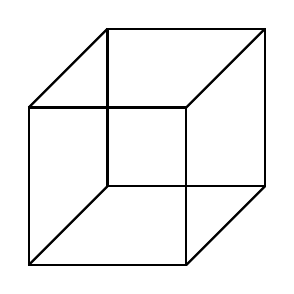
\begin{tikzpicture}
	\draw [thick] (0,0) rectangle (2,2);
	\draw [thick] (1,1) rectangle (3,3);
	\draw [thick] (0,0) -- (1,1);
	\draw [thick] (0,2) -- (1,3);
	\draw [thick] (2,2) -- (3,3);
	\draw [thick] (2,0) -- (3,1);
\end{tikzpicture}
\column{.3\textwidth}
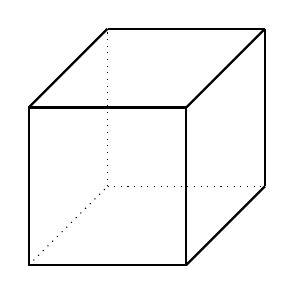
\begin{tikzpicture}
	\draw [thick] (0,0) rectangle (2,2);
	%\draw [thick] (1,1) rectangle (3,3);
	\draw [dotted] (0,0) -- (1,1);
	\draw [dotted] (1,1) -- (1,3);
	\draw [dotted] (1,1) -- (3,1);
	\draw [thick] (1,3) -- (3,3);
	\draw [thick] (3,1) -- (3,3);
	\draw [thick] (0,2) -- (1,3);
	\draw [thick] (2,2) -- (3,3);
	\draw [thick] (2,0) -- (3,1);
\end{tikzpicture}
\column{.3\textwidth}
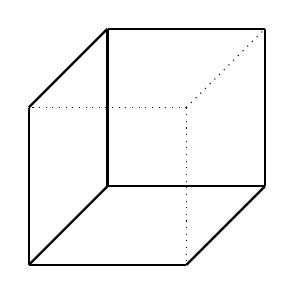
\begin{tikzpicture}
	\draw [thick] (0,0) -- (1,1);
	\draw [thick] (0,0) -- (0,2);
	\draw [thick] (0,0) -- (2,0);
	\draw [thick] (1,1) -- (1,3);
	\draw [thick] (1,1) -- (3,1);
	\draw [thick] (1,3) -- (3,3);
	\draw [thick] (3,1) -- (3,3);
	\draw [thick] (0,2) -- (1,3);
	\draw [dotted] (2,2) -- (3,3);
	\draw [dotted] (2,2) -- (0,2);
	\draw [dotted] (2,2) -- (2,0);
	\draw [thick] (2,0) -- (3,1);
\end{tikzpicture}
\end{columns}
\begin{figure}
	\includegraphics[width=.3\textwidth,angle=0,origin=c]{img/duck-rabbit.png}
	\includegraphics[width=.3\textwidth,angle=0,origin=c]{img/old-beauty.png}
	\includegraphics[width=.3\textwidth,angle=0,origin=c]{img/vase-face.png}
\end{figure}
\end{frame}

\begin{frame}\frametitle{Monotone Kolmogorov Complexity}
	\begin{definition}[Monotone Kolmogorov Complexity]
	\[Km(x)\coloneqq \min\limits_p\{\ell(p): U(p)=x*\}\]
	where $U$ is a universal monotone Turing machine.
	\end{definition}
	\begin{itemize}
		\item $Km(x)\leqa\ell(x)$
		\item $Km(xy)\geq Km(x)$
		\item $Km(x)\leqa -\log\mu(x)+K(\mu)$ if $\mu$ is a computable measure
	\end{itemize}
It is natural to call an infinite sequence $\omega$ computable if $Km(\omega)<\infty$.
\end{frame}

\begin{frame}\frametitle{Algorithmic Coding Theorem}
		%\setlength\abovedisplayskip{0pt}
		%\setlength\belowdisplayskip{0pt}
	\begin{block}{}
	\[m(x)\coloneqq \sum\limits_{p:U(p)\downarrow=x}2^{-\ell(p)}\]
	\end{block}
	\begin{theorem}[Algorithmic Coding Theorem]
		\[K(x)\,\eqa\,-\log m(x)\]
	\end{theorem}
	The probability of a string being produced by a random algorithm is inversely proportional to its algorithmic complexity.\\
	If a string has many long descriptions then it also has a short description.
	\[KM(x)\coloneqq -\log M(x)\]
	\[0\leq K(x\mid \ell(x))\leqa KM(x)\leq Km(x)\leq K(x)\leqa\ell(x)+2\log\ell(x)\]
\end{frame}

\begin{frame}\frametitle{Occam's Razor}
	\[M(y\mid x)\approx 2^{-K(y\mid x)}\]
	\textbf{Remark:} Occam's razor --- $M$ predicts $y$ with high probability iff $y$ has an easy explanation, given $x$.
\end{frame}

\begin{frame}\frametitle{(Semi)Measure}
\begin{definition}[(Semi)Measure]
We call $\rho:\mathcal{X}^*\to[0,1]$ a semimeasure if $\rho(\epsilon)\leq 1$ and $\rho(x)\geq\sum\limits_{a\in\mathcal{X}}\rho(xa)$, and a probability measure if equality holds.
\end{definition}
\[\rho(x_t\mid x_{<t})\coloneqq\frac{\rho(x_{1:t})}{\rho(x_{<t})}\]
\[\rho(x_1\dots x_n)=\rho(x_1)\rho(x_2\mid x_1)\dots\rho(x_n\mid x_1\dots x_{n-1})\]
\begin{block}{}
$\rho$ is an lower semicomputable semimeasure iff there is a monotone Turing machine $T$ s.t. 
\[\rho(x)=\sum\limits_{p:T(p)=x*}2^{-\ell(p)}\quad\mbox{and}\quad\ell(\langle T\rangle)\eqa K(\rho)\]
where $T(p)=U(\langle T\rangle p)$.	
\end{block}
\end{frame}

\begin{frame}\frametitle{Simple Deterministic Bound}
Sequence prediction algorithms try to predict the continuation $x_t$ of a given sequence $x_1\dots x_{t-1}$.
\begin{theorem}
\[
\sum\limits_{t=1}^\infty\big|1-M(x_t\mid x_{<t})\big| \leq Km(x_{1:\infty})\ln 2
\]
\end{theorem}
\begin{proof}
\[\sum\limits_{t=1}^\infty\big|1-M(x_t\mid x_{<t})\big| \leq -\sum\limits_{t=1}^\infty\ln M(x_t\mid x_{<t}) = -\ln M(x_{1:\infty}) \leq Km(x_{1:\infty})\ln2 \]
\end{proof}
\end{frame}

\begin{frame}\frametitle{Solomonoff's Completeness Theorem}
	\begin{align*}
	M'(\epsilon)&\coloneqq 1\\
	M'(x_{1:t})&\coloneqq M'(x_{<t})\frac{M(x_{1:t})}{\sum\limits_{x\in\mathcal{X}}M(x_{<t}x)}=\frac{M(x_{1:t})}{M(\epsilon)}\prod\limits_{i=1}^t\frac{M(x_{<i})}{\sum\limits_{x\in\mathcal{X}}M(x_{<i}x)}
	\end{align*}
	\begin{theorem}[Solomonoff's Completeness Theorem]
		For any computable measure $\mu$,
		\[\sum\limits_{t=1}^\infty\sum\limits_{x_{1:t}\in\mathcal{X}^t}\mu(x_{<t})\Big(M'(x_t\mid x_{<t})-\mu(x_t\mid x_{<t})\Big)^2\leq D(\mu\|M) \leqa K(\mu)\ln2\]
	\end{theorem}
\textbf{Remark:} $M'$ is universal predictor. The only assumption made is that data are generated from a computable distribution.
\end{frame}

\begin{frame}\frametitle{Prediction Bounds}
\setlength\abovedisplayskip{0pt}
\setlength\belowdisplayskip{0pt}
\begin{theorem}[Total Bounds]
\[
 \sup_{A\subseteq\mathcal{X}^\infty} \big|M(A\mid x_{<t})-\mu(A\mid x_{<t})\big| \xrightarrow[w.\mu.1]{t\to\infty} 0
\]
\end{theorem}
\begin{theorem}[Instantaneous Bounds]
\[
 2^{-K(n)} \;\leq\; (1-M(x_n\mid x_{<n})) \;\leq\; C\cdot 2^{-K(n)}
\]
\end{theorem}
e.g. $M(0\mid 1^n) \;\eqm\; 2^{-K(n)}\to 0$
\begin{theorem}[Future Bounds]
\[
 \sum\limits_{t=n+1}^\infty \mathbb{E}_\mu\left[\left.\sum\limits_{a\in\mathcal{X}}\left(\sqrt{\xi(a\mid x_{1:t})}-\sqrt{\mu(a\mid x_{1:t})}\right)^2\right|x_{1:n}\right] \;\leqa\; \big(K(\mu\mid x_{1:n})+K(n)\big)\ln 2
\]
\end{theorem}
\begin{theorem}[Universal is Better than Continuous $\mathcal{M}$]
\[
 D_n(\mu\|M)\coloneqq \mathbb{E}_\mu\left[\ln\frac{\mu}{M}\right]=\mathbb{E}_\mu\left[\ln\frac{\mu}{\xi}\right]+\mathbb{E}_\mu\left[\ln\frac{\xi}{M}\right] \;\leqa\; D_n(\mu\|\xi)+K(\xi)\ln2
\]
\end{theorem}
\end{frame}

\begin{frame}\frametitle{}
\begin{itemize}
	\item For continuous $\mathcal{M}$, we can assign a universal prior (not density)
	\[w_\theta^U\coloneqq
	\begin{cases}
		2^{-K(\theta)} & \mbox{if $\theta$ is computable}\\
		0 & \mbox{otherwise}
	\end{cases}
	\]
	\item This effectively reduces $\mathcal{M}$ to a discrete class $\left\{\nu_\theta\in\mathcal{M}: w_\theta^U>0\right\}$ which is typically dense in $\mathcal{M}$.
\end{itemize}
\end{frame}

\begin{frame}\frametitle{Emergence of Simple Laws of Physics}
\begin{block}{Completeness Theorem}
	For any computable measure $\mu$, there is a set $A\subset\mathcal{X}^*$ with $\mu(A)=1$ s.t. for all $\mathbf{x}\in A$
	\[\sum\limits_{y\in\mathcal{X}}\Big(\sqrt{M'(y\mid\mathbf{x})}-\sqrt{\mu(y\mid\mathbf{x})}\Big)^2\xrightarrow{n\to\infty}0\]
\end{block}
\begin{block}{Emergence of Simple Laws of Physics}
	For any computable measure $\mu$,
	\[M'\left\{\sum\limits_{y\in\mathcal{X}}\Big(\sqrt{M'(y\mid\mathbf{x})}-\sqrt{\mu(y\mid\mathbf{x})}\Big)^2\xrightarrow{n\to\infty}0\right\}\geq 2^{-K(\mu)}\]
\end{block}
\centerline{\fbox{\textcolor{red}{Why is there a `world' with simple laws?}}}
\centerline{\fbox{\textcolor{red}{Assume observers/observations are fundamental. $P(o_\mathrm{future}\mid o_\mathrm{past})$}}}
\end{frame}

\begin{frame}\frametitle{Emergence of Simple Laws of Physics}
\begin{figure}[H]
\includegraphics[height=.33\textwidth]{img/it-bit.pdf}
\includegraphics[height=.33\textwidth]{img/wheeleru.jpeg}
\end{figure}
\[M'\left\{\sum\limits_{y\in\mathcal{X}}\Big(\sqrt{M'(y\mid\mathbf{x})}-\sqrt{\mu(y\mid\mathbf{x})}\Big)^2\xrightarrow{n\to\infty}0\right\}\geq 2^{-K(\mu)}\]
\centerline{\fbox{\textcolor{red}{Why is there a `world' with simple laws?}}}
\centerline{\fbox{\textcolor{red}{Assume observers/observations are fundamental. $P(o_\mathrm{future}\mid o_\mathrm{past})$}}}
\textbf{Kant's Copernican Revolution:} The understanding does not derive its laws from, but prescribes them to, nature.
\end{frame}

\begin{frame}\frametitle{``The Universe is made of stories, not of atoms.''}
\begin{itemize}
	\item Understanding is \textcolor{red}{compression}! To comprehend is to compress!
	\item To find meaning in our lives, \textcolor{red}{we tell ourselves stories}. We explain our lives through patterns.
	\item Is the story \textcolor{red}{true}? It's a conspiracy! Fusion of horizons!
	\item Can there be a \textcolor{red}{better} story that is more exact? Maybe. Maybe not.
	\item Is the story the \textcolor{red}{best} one? We never know!\\
	\begin{itemize}
		\item[---] Kolmogorov complexity $K$ is uncomputable.
	\end{itemize}
	\item What is a \textcolor{red}{good} story?
\begin{enumerate}
	\item varifiable/falsifiable,
	\item hard to vary,
	\item simple in hypotheses,
	\item rich in phenomena/applicability/conclusions.
\end{enumerate}
\end{itemize}
\end{frame}

\begin{frame}\frametitle{Universal Prediction of Selected Bits}
	\begin{theorem}[Universal Prediction of Selected Bits]
		Let $f:\{0,1\}^*\to\{0,1,\epsilon\}$ be a total recursive function and $x\in 2^\omega$ satisfying $f(x_{<n})=x_n$ whenever $f(x_{<n})\neq\epsilon$. If $f(x_{<n_i})\neq\epsilon$ for an infinite sequence $n_1,n_2,\dots$ then
		\[\lim\limits_{i\to\infty}M'(x_{n_i}\mid x_{<n_i})=1\]
	\end{theorem}
\end{frame}

\begin{frame}\frametitle{Pure Universal Inductive Logic?}
\setlength\abovedisplayskip{0pt}
\setlength\belowdisplayskip{0pt}
\begin{block}{}
\begin{itemize}
\item $M(\Theta(a_{1:n}))\coloneqq \sum\limits_{p:U(p)=h_{1:n}*}2^{-\ell(p)}$\\
where $\Theta(a_{1:n})\coloneqq \bigwedge\limits_{i=1}^n Q_{h_i}(a_i)$.
\item $M'\left(A(\vec{a})\right)\coloneqq \sum\limits_{\Theta(\vec{b})\vDash A(\vec{a})} M'(\Theta(\vec{b}))$\\
where
$\vDash A(\vec{a})\leftrightarrow\bigvee\limits_{\Theta(\vec{b}) \vDash A(\vec{a})}\Theta(\vec{b}). \hfill\text{FDNF}$
\end{itemize}
\end{block}
\centerline{\fbox{$\sum\limits_{t=1}^\infty\sum\limits_{A(a_{1:t})}\mu\left(A(a_{<t})\right)\Big(M'\left(A(a_t)\,\middle|\, A(a_{<t})\right)-\mu\left(A(a_t)\,\middle|\, A(a_{<t})\right)\Big)^2\leqa K(\mu)\ln 2$}}
where $A(a_{1:t})\coloneqq \bigwedge\limits_{i=1}^t A(a_i/x)$.
\end{frame}

\begin{frame}\frametitle{All Ravens are Black!~$\checkmark$}
	\begin{theorem}[All Ravens are Black]
		\[\lim\limits_{n\to\infty} M'\left(\forall x(R(x)\to B(x))\,\middle|\,\bigwedge\limits_{i=1}^n (\neg R(a_i)\vee B(a_i))\right)=1\]
	\end{theorem}
	\begin{theorem}[Confirmation by Random Sampling]
		If the sampling function $t:\mathbb{N}\to\mathbb{N}$ satisfies $\forall i: t_i\leq t_{i+1}$ and $\chi_{1:\infty}$ is Martin-L\"of random, where $\chi_i\coloneqq \llbracket\exists k(t_k=i)\rrbracket$, then
		\[M'\left(\forall x A(x)\,\middle|\,\bigwedge\limits_{i=1}^n A(a_{t_i})\right)\xrightarrow{n\to\infty}1\]
	\end{theorem}
	\[M(1\mid 1^n)\xrightarrow{n\to\infty}1\qquad M(0\mid 1^n)\eqm 2^{-K(n)}\qquad\sum\limits_{n=0}^\infty M(0\mid 1^n)<\infty\]
\end{frame}

%--------------------------%
\subsection{A Statistical Mechanical Interpretation of AIT}
%--------------------------%

\begin{frame}\frametitle{\href{http://www2.odn.ne.jp/tadaki}{A statistical mechanical interpretation of AIT --- Tadaki}}
\begin{table}
\abovetabulinesep=1mm
\belowtabulinesep=1mm
\begin{tabu}{lll}
	an energy eigenstate $n$ &$\implies$ &a program $p$ s.t. $U(p)\downarrow$\\
	the energy $E_n$ of $n$ &$\implies$ &the length $\ell(p)$ of $p$\\
	Boltzmann constant $k$ &$\implies$ &$1/\ln 2$
\end{tabu}
\end{table}
\begin{table}%\renewcommand\arraystretch{2}
\abovetabulinesep=1.5mm
\belowtabulinesep=1.5mm
\begin{tabu}{llll}
	\Xhline{1pt}
	$Z=\sum\limits_n\! e^{-\frac{E_n}{kT}}$ & $\implies$ & $Z=\textcolor{red}{\sum\limits_{p:U(p)\downarrow}\!\!2^{-\frac{\ell(p)}{T}}}$ & \text{Partition function}\\
	$F=-kT\ln Z$ & $\implies$ &$F=-T\log Z$ &\text{Free energy}\\
	$P(n)=\dfrac{1}{Z}e^{-\frac{E_n}{kT}}$ & $\implies$ & $P(p)=\dfrac{1}{Z}2^{-\frac{\ell(p)}{T}}$ & \text{Boltzmann distribution}\\
	$E=\sum\limits_n\! P(n)E_n$ & $\implies$ & $E=\!\sum\limits_{p:U(p)\downarrow}\!\!P(p)\ell(p)$ & \text{Energy}\\
	$S=\dfrac{E-F}{T}$ & $\implies$ & $S=\dfrac{E-F}{T}\textcolor{red}{=H(P)}$ & \text{Entropy}\\
	$C=\dfrac{\mathrm{d}E}{\mathrm{d}T}$ & $\implies$ & $C=\dfrac{\mathrm{d}E}{\mathrm{d}T}$ & \text{Specific heat}\\
	\Xhline{1pt}
\end{tabu}
\end{table}
\end{frame}

\begin{frame}\frametitle{Temperature $=$ Compression Rate}
\begin{theorem}
\begin{enumerate}
\item If $0<T<1$ and $T$ is computable, then each of $Z,F,E,S,C$ converges to a real whose compression rate equals to $T$, i.e.
\[\resizebox{.95\textwidth}{!}{$\lim\limits_{n\to\infty}\frac{K(Z_{1:n})}{n}=\lim\limits_{n\to\infty}\frac{K(F_{1:n})}{n}=\lim\limits_{n\to\infty}\frac{K(E_{1:n})}{n}=\lim\limits_{n\to\infty}\frac{K(S_{1:n})}{n}=\lim\limits_{n\to\infty}\frac{K(C_{1:n})}{n}=T$}\]
\item If $T>1$, then $Z=E=S=\infty$, and $F=-\infty$.
\item If $T=1$, then $Z,F$ converge, but $E=S=C=\infty$.
\end{enumerate}
\end{theorem}
\end{frame}

\begin{frame}\frametitle{Fixpoint Theorem on Compression Rate}
\begin{theorem}[Fixpoint Theorem on Compression Rate]
For every $T\in(0,1)$, if $Z$ or $F$ is computable, then
\[\lim\limits_{n\to\infty}\frac{K(T_{1:n})}{n}=T\]
\end{theorem}
\begin{block}{Intuitive Meaning}
Consider a file of infinite size whose content is
\[\mbox{``The compression rate of this file is $0.100111001\dots\dots$''}\]
When this file is compressed, the compression rate of this file actually equals to $0.100111001\dots\dots$, as the content of this file says.\\
\centerline{This situation forms a fixpoint and is self-referential.}	
\end{block}
\begin{theorem}
There does not exist $T\in(0,1)$ such that both $Z$ and $F$ are computable.
\end{theorem}
\end{frame}

\begin{frame}\frametitle{\href{https://arxiv.org/abs/1010.2067}{A Similar Version --- Baez \& Stay}}
\begin{table}\renewcommand\arraystretch{1.8}
\begin{tabu}{ll}
\Xhline{1pt}
$E_{\{p\}}=\ln t(p)$ & Energy\\
$V_{\{p\}}=\ell(p)$ & Volume\\
$N_{\{p\}}=U(p)$ & Number of molecules\\
$Z=\sum\limits_{p:U(p)\downarrow} \mathrm{e}^{-\frac{E_{\{p\}}+PV_{\{p\}}-\mu N_{\{p\}}}{T}}$ & Partition function \\
$P(p)=\dfrac{1}{Z}\mathrm{e}^{-\frac{E_{\{p\}}+PV_{\{p\}}-\mu N_{\{p\}}}{T}}$ & Boltzmann distribution \\
\Xhline{1pt}
\end{tabu}
\end{table}
{\footnotesize
\begin{itemize}
	\item \textcolor{yellow}{Temperature} $T$: how many times you must double the runtime in order to double the number of programs in the ensemble while holding their mean length and output fixed.
	\item \textcolor{yellow}{Pressure} $P$ : how much you need to decrease the mean length to increase the mean log runtime by a specified amount, while holding the number of programs in the ensemble and their mean output fixed.
	\item \textcolor{yellow}{Potential} $\mu$: how much the mean log runtime increases when you increase the mean output while holding the number of programs in the ensemble and their mean length fixed.
\end{itemize}}
\end{frame}

\begin{frame}\frametitle{Variant$1$}
\begin{table}\renewcommand\arraystretch{2}
\begin{tabu}{ll}
	\Xhline{1pt}
	$E_{\{p,h\}}=\begin{cases}
		\ell(p) &\mbox{if } U(p)=h*\\
		0 &\mbox{otherwise}
	\end{cases}$ & Energy of $(p,h)$\\
	$Z(h)=\textcolor{red}{\sum\limits_{p:U(p)=h*}\!\!2^{-\frac{\ell(p)}{T_h}}}\textcolor{red}{=M(h)}$ & \text{Partition function}\\
	$F(h)=-T_h\log Z(h)$ & \text{Free energy}\\
	$P_h(p)=\dfrac{1}{Z(h)}2^{-\frac{E_{\{p,h\}}}{T_h}}$ & \text{Boltzmann distribution}\\
	$E(h)=\!\sum\limits_{p:U(p)=h*}\!\!P_h(p)E_{\{p,h\}}$ & \text{Energy}\\
	$S(h)=\dfrac{E(h)-F(h)}{T_h}\textcolor{red}{=H(P_h)}$ & \text{Entropy}\\
	\Xhline{1pt}
\end{tabu}
\end{table}
If we take temperature as compression rate $T_h\coloneqq\frac{K(h)}{\ell(h)}$.
\end{frame}

\begin{frame}\frametitle{Variant$2$}
\vspace*{-4ex}
\begin{table}\renewcommand\arraystretch{1.3}\hspace*{-2ex}
\begin{tabu}{ll}
	\Xhline{1pt}
	$E_{\{p,h\}}=\begin{cases}
		\log t(p,h) &\mbox{if } U(p)=h*\\
		0 &\mbox{otherwise}
	\end{cases}$ & Internal energy of $(p,h)$\\
	$V_{\{p,h\}}=\begin{cases}
		\ell(p) &\mbox{if } U(p)=h*\\
		0 &\mbox{otherwise}
	\end{cases}$ & Volume of $(p,h)$\\	
	$H_{\{p,h\}}=E_{\{p,h\}}+PV_{\{p,h\}}$ & \text{Enthalpy of $(p,h)$, \footnotesize{where $P$ is pressure}}\\
	$Z(h)=\textcolor{red}{\sum\limits_{p:U(p)=h*}\!\!2^{-\frac{H_{\{p,h\}}}{T_h}}}$ & \text{Partition function}\\
	$F(h)=-T_h\log Z(h)$ & \text{Free energy}\\
	$P_h(p)=\dfrac{1}{Z(h)}2^{-\frac{H_{\{p,h\}}}{T_h}}$ & \text{Boltzmann distribution}\\
	$E(h)=\!\sum\limits_{p:U(p)=h*}\!\!P_h(p)E_{\{p,h\}}$ & \text{Energy}\\
	$V(h)=\!\sum\limits_{p:U(p)=h*}\!\!P_h(p)V_{\{p,h\}}$ & \text{Volume}\\
	$S(h)=\dfrac{E(h)+PV(h)-F(h)}{T_h}\textcolor{red}{=H(P_h)}$ & \text{Entropy}\\
	\Xhline{1pt}
\end{tabu}
\end{table}
\end{frame}

\begin{frame}\frametitle{Computable Universal Predictor}
\[Z(h)=\sum\limits_{p:U(p)=h*}\!\!2^{-\frac{\textcolor{red}{\ell(p)+\log t(p,h)}}{T}}\]
\begin{theorem}
If $T_h$ is computable, Then $Z(h)$ is a computable semimeasure.
\end{theorem}
\[\sum\limits_{t=1}^\infty\big|1-Z(h_t\mid h_{<t})\big|\leq \dfrac{Km(h)\ln 2+\ln t(p,h)}{T_h}\]
\end{frame}

\begin{frame}\frametitle{Variant$3$ --- Stochastic Case}
\begin{table}\renewcommand\arraystretch{1.8}
\begin{tabu}{ll}
	\Xhline{1pt}
	$E_{\{\nu,h\}}^{\mathrm{in}}= 
\begin{cases}
-\log w_\epsilon^\nu & \mbox{if } \nu\in\mathcal{M}_h\\
0 & \mbox{otherwise}
\end{cases}$ & Internal energy\\
	$E_{\{\nu,h\}}^{\mathrm{ex}}= 
\begin{cases}
-\log\nu(h) & \mbox{if } \nu\in\mathcal{M}_h\\
0 & \mbox{otherwise}
\end{cases}$ & External energy\\
	$E_{\{\nu,h\}} = E_{\{\nu,h\}}^{\mathrm{in}}+E_{\{\nu,h\}}^{\mathrm{ex}}$ & Total energy\\
	$Z(h) = \sum\limits_{\nu\in\mathcal{M}_h}2^{-\frac{E_{\{\nu,h\}}}{T_h}}$ & \text{Partition function}\\
	$F(h) = -T_h\log Z(h)$ & \text{Free energy}\\
	$P_h(\nu) = \dfrac{1}{Z(h)}2^{-{\frac{E_{\{\nu,h\}}}{T_h}}}$ & \text{Boltzmann distribution}\\
	$E(h) = \sum\limits_{\nu\in\mathcal{M}_h}P_h(\nu)E_{\{\nu,h\}}$ & \text{Average Energy}\\
	$S(h)=\dfrac{E(h)-F(h)}{T_h}\textcolor{red}{=H(P_h)}$ & \text{Entropy}\\
	\Xhline{1pt}
\end{tabu}
\end{table}
\end{frame}

\begin{frame}\frametitle{Stochastic Case}
If $T_h=1$, then
\[E_{\{\nu,h\}}=-\log w_\epsilon^\nu-\log\nu(h)\]
\[Z_h=\sum\limits_{\nu\in\mathcal{M}}2^{-E_{\{\nu,h\}}}=\sum\limits_{\nu\in\mathcal{M}}w_\epsilon^\nu\nu(h)=\xi(h)\]
\[P_h(\nu)=\frac{2^{-E_{\{\nu,h\}}}}{Z_h}=\frac{w_\epsilon^\nu\nu(h)}{\xi(h)}=w_h^\nu\]
\begin{align*}
F_h=-\log Z_h=\underbrace{-\log\xi(h)}_{\approx K(h)}&=\mathbb{E}_{w_\epsilon}\left[E_{\{\nu,h\}}^{\mathrm{ex}}\right]-D(w_\epsilon\|w_h)\\
&=\mathbb{E}_{w_h}\left[E_{\{\nu,h\}}^{\mathrm{ex}}\right]+D(w_h\|w_\epsilon)\\
&=\underbrace{\mathbb{E}_{w_h}[-\log\nu(h)]}_{\textit{noise}}+\underbrace{D(w_h\|w_\epsilon)}_{\textit{surprise}}
\end{align*}
\begin{align*}
	H(P_h)&=H(w_h)=\underbrace{H(w_h,w_\epsilon)}_{\textit{cross entropy}}-D(w_h\|w_\epsilon)
\end{align*}
\end{frame}

\begin{frame}\frametitle{}
\begin{quote}
``What an organism feeds upon is negative entropy.''\par
\hfill --- \textsl{Schr\"odinger}
\end{quote}
\begin{quote}
``Every living thing is a sort of imperialist, seeking to transform as much as possible of its environment into itself and its seed.''\par
\hfill --- \textsl{Russell}
\end{quote}
\end{frame}

\begin{frame}\frametitle{Intrinsic Utility}
	\begin{itemize}
		\item \textcolor{green}{square} \textcolor{yellow}{$-\xi(e_{t:k}\mid\ae_{<t}a_{t:k})$}
		\item \textcolor{green}{Shannon} \textcolor{yellow}{$-\log\xi(e_{t:k}\mid \ae_{<t}a_{t:k})\approx K(\ae_{1:k})-K(\ae_{<t})$}
		\item \textcolor{green}{KL divergence} $\textcolor{yellow}{D\left(w_{\ae_{<k}}\|w_{\ae_{<t}}\right)}$ where $w_{\ae_{<n}}^\nu=\dfrac{w_\nu\nu(e_{<n}\mid a_{<n})}{\xi(e_{<n}\mid a_{<n})}$
		\item \textcolor{green}{information gain} $\textcolor{yellow}{H(w_{h_{<t}})-H(w_{h_{1:k}})}$ where \[H(w_h)\coloneqq -\sum\limits_{\nu\in\mathcal{M}}w_h^\nu\log w_h^\nu\]
		\item \textcolor{green}{effective complexity} $\textcolor{yellow}{\mathcal{E}_\delta(\ae_{1:k})-\mathcal{E}_\delta(\ae_{<t})}$ where
		\[\mathcal{E}_\delta(\ae_{<n})\coloneqq \min\limits_{\nu\in\mathcal{M}}\left\{2K(\nu)+H(\nu)-K(\ae_{<n}): \nu(e_{<n}\mid a_{<n})\geq 2^{-H(\nu)(1+\delta)}\right\}\]
		\item \textcolor{green}{logical depth} $\textcolor{yellow}{\operatorname{depth}_b(h_{1:k})-\operatorname{depth}_b(h_{<t})}$ where
		\[\operatorname{depth}_b(x)\coloneqq \min\left\{t: U^t(p)=x\;\;\&\;\;\ell(p)-K(x)\leq b\right\}\]
	\end{itemize}
\end{frame}



\begin{frame}\frametitle{Occam's Razor vs Maximum Entropy}
\[\textcolor{red}{\mathop{minimize}\limits_{w\vDash\left\{
			{\scalebox{.5}{$\begin{aligned}
				&H(w)=C\\
				&\sum\limits_{\nu\in\mathcal{M}}w_\nu=1
				\end{aligned}$}}\right.} \sum\limits_{\nu\in\mathcal{M}}w_\nu K(\nu)}\qquad \mbox{or}\quad\mathop{maximize}\limits_{w\vDash\left\{
			{\scalebox{.5}{$\begin{aligned}
				&\sum\limits_{\nu\in\mathcal{M}}w_\nu K(\nu)=C\\
				&\sum\limits_{\nu\in\mathcal{M}}w_\nu=1
				\end{aligned}$}}\right.} H(w)\]
\[
L\coloneqq\sum\limits_{\nu\in\mathcal{M}}w_\nu K(\nu)-T\left(-\sum\limits_{\nu\in\mathcal{M}}w_\nu\log w_\nu-C\right)-\lambda\left(\sum\limits_{\nu\in\mathcal{M}}w_\nu-1\right)
\]
\[\dfrac{\partial L}{\partial w_\nu}=0\implies \textcolor{red}{w_\nu^T=\dfrac{2^{-\frac{K(\nu)}{T}}}{\sum\limits_{\nu\in\mathcal{M}}2^{-\frac{K(\nu)}{T}}}}\]
\[\fbox{If the temperature $0<T<1$, then the Shannon entropy $H(w^T)<\infty$.}\]
\end{frame}

\begin{frame}\frametitle{Why Solomonoff Prior?}
\[H(w)\leq\mathbb{E}_w[K]\leq H(w)+K(w)\]
\begin{block}{}
\centerline{Maximum Entropy + Occam's Razor}
\end{block}
\[T\coloneqq \dfrac{\mathbb{E}_w[K]}{H(w)}\]
\[
\mathop{minimize}\limits_{w\vDash\sum\limits_{\nu\in\mathcal{M}}\!w_\nu=1} T \implies
w_\nu=\dfrac{2^{\frac{-K(\nu)}{T}}}{\sum\limits_{\nu\in\mathcal{M}}2^{\frac{-K(\nu)}{T}}}
\]
If $w$ is lower semicomputable then
\[K(w)<\infty\implies T=1\implies w_\nu^*=\dfrac{2^{-K(\nu)}}{\sum\limits_{\nu\in\mathcal{M}}2^{-K(\nu)}}\]
\end{frame}

\begin{frame}\frametitle{Zipf's Law}
	\[p_k\propto k^{-1}\]
\begin{align*}
p_k &= \mbox{frequency of a word of rank } k\\
k &= \mbox{rank of a word (if sorted by frequency)}
\end{align*}
\begin{itemize}
	\item $C_k$: a certain ``cost'' of the word of rank $k$
	\item the average cost per word $C\coloneqq\sum_k p_k C_k$
	\item the entropy $H\coloneqq -\sum_kp_k\log p_k$
	\item $T\coloneqq\frac{C}{H}$
	\item $\operatorname{minimize} T\implies p_k\propto 2^{-\frac{C_k}{T}}$
	\item if $C_k=\log k$, then $p_k\propto k^{-\frac{1}{T}}$
\end{itemize}
\end{frame}

\begin{frame}\frametitle{Advantages \& Disadvantages}
	\begin{itemize}
		\item \textcolor{yellow}{free-lunch}
		\item \textcolor{yellow}{universality --- finite error}
		\item \textcolor{yellow}{data sparse problem --- arbitrary order Markov chain --- universal smoothing method}
		\item \textcolor{yellow}{confirmation of $\forall x: R(x)\to B(x)$}
		\item \textcolor{red}{incomputability}
		\item \textcolor{red}{weakly depends on universal Turing machine}
	\end{itemize}
\end{frame}

%--------------------------%
\subsection{Incompressibility \& Incompleteness}
%--------------------------%

\begin{frame}\frametitle{Halting Problem}
\setlength\abovedisplayskip{0pt}
\setlength\belowdisplayskip{0pt}
	\begin{theorem}[Halting Problem is Undecidable]
		There is no computable function deciding whether a program halts.
	\end{theorem}
\begin{columns}
\column{.48\textwidth}
\begin{proof}
	Assume there exists a halting program $H$.\\
	Construct a program $q$ as follows: 
	\begin{enumerate}
		\item read $n$;
		\item generate $A\coloneqq \{p:\ell(p)\leq n\}$;
		\item use $H$ to get $B\coloneqq \{p\in A: U(p)\downarrow\}$;
		\item output $2\max\{U(p): p\in B\}$.
	\end{enumerate}
\[\ell(q)\leqa\log n\lesssim n\implies U(q)\geq 2U(q)\]
\end{proof}
\column{.5\textwidth}
\begin{figure}[H]
	\includegraphics[width=1.45\textwidth]{img/halt-wait}
\end{figure}
\end{columns}
\end{frame}

\begin{frame}\frametitle{Incompressibility vs Incompleteness vs Berry Paradox}
	\begin{theorem}[Kolmogorov]
		Kolmogorov complexity $K$ is uncomputable.
	\end{theorem}\vspace{-11pt}
	\[x^*\coloneqq \mu x[K(x)>n]\implies n<K(x^*)\leq O(\log n)\]
	\begin{theorem}[Chaitin]
		For any arithmetically sound G\"odelian $\mathrm{T}$, $\exists c\forall x: \mathrm{T}\nvdash K(x)>c$.
	\end{theorem}\vspace{-17pt}
	\[\textcolor{green}{\mbox{``given $n$, find $\mu y\big[\operatorname{prf}_\mathrm{T}\big(y,K(x)>n\big)\big]$, ouput $x$''}}\implies n<K(x)\leq O(\log n)\]
	{\centering\small \textcolor{yellow}{``the least number undefinable in fewer characters than there are in this sentence.''}}
	\[\mbox{\textcolor{yellow}{$M_e\coloneqq $``find $\mu y\big[\operatorname{prf}_\mathrm{T}\big(y,K(x)>e\big)\big]$, ouput $x$'' \tag{Berry Paradox}}}\]
	\begin{theorem}[Chaitin]
		For any arithmetically sound G\"odelian $\mathrm{T}$, $\big|\big\{x: \mathrm{T}\vdash K(x)>\ell(x)\big\}\big|<\infty$.
	\end{theorem}
\end{frame}

\begin{frame}\frametitle{Incompressibility vs Incompleteness vs Berry Paradox}
\setlength\abovedisplayskip{0pt}
\setlength\belowdisplayskip{0pt}
	\begin{definition}[Kolmogorov Complexity $H$]
		\begin{align*}
		H(x\mid y)&\coloneqq \mu e[\varphi_e(y)=x]\\
		H(x)&\coloneqq H(x\mid \epsilon)
		\end{align*}
	\end{definition}
	\begin{theorem}[Chaitin]
		For any arithmetically sound G\"odelian $\mathrm{T}$, $\exists c\forall x: \mathrm{T}\nvdash H(x)>c$.
	\end{theorem}
	\begin{proof}
		For any $m$, construct:
		\[M_n\coloneqq \text{``find}\;\mu y\big[\operatorname{prf}_\mathrm{T}\big(y,H(x)>m\big)\big], \text{output $x$''}\]
		Then there exists a computable $f: m\mapsto n$.\\
		By Kleene's fixpoint theorem,
		\[\exists e: M_e=M_{f(e)}=\text{``find}\;\mu y\big[\operatorname{prf}_\mathrm{T}\big(y,H(x)>e\big)\big], \text{output $x$''}\]
		Take $c\coloneqq e$.
	\end{proof}
\end{frame}

\begin{frame}\frametitle{\href{http://www.vetta.org/documents/Machine_Super_Intelligence.pdf}{Incompressibility vs Incompleteness vs Intelligence}}
	\begin{columns}
		\column{\textwidth}
			\begin{itemize}
				\item $P(x)\coloneqq \big\{p\in\mathcal{X}^*:\exists m\forall n\geq m\left(p(x_{1:n})=x_{n+1}\right)\big\}$
				\item $P(A)\coloneqq \bigcap\limits_{x\in A}P(x)$
				\item $P_n\coloneqq P\big(\big\{x: Km(x)\leq n\big\}\big)$
			\end{itemize}\vspace{17ex}
			\begin{minipage}{.6\textwidth}
				\begin{itemize}
					\item $\forall n\exists p\in P_n: K(p)\leqa n+O(\log n)$
					\item $\forall n: p\in P_n\Longrightarrow K(p)\geqa n$
				\end{itemize}
			\end{minipage}
		\column{.75\textwidth}\vspace{-1.3cm}
			\resizebox{.11\textwidth}{!}{\hspace{-8cm}
				\begin{minipage}{\textwidth}
					\begin{figure}
						\centering\begin{tikzpicture}
						%\draw [help lines] (0,0) grid (10,5);
						\draw[->,very thick] (0,0) -- (0,5);
						\draw[-,very thick,green] (0,0) -- (5.5,3);
						\draw[->,very thick] (0,0) -- (5.5,0);
						\draw[-,very thick,red] (2,0) -- (2,5);
						
						\node at (-0.7,0.3) {$\text{simple}\atop{\text{algorithms}}$};
						\node at (-0.7,4.5) {$\text{complex}\atop{\text{algorithms}}$};
						\node at (0.3,-0.5) {weak AI};
						\node at (4.9,-0.5) {powerful AI};
						\node at (2,-0.5) {$\text{upper bound}\atop{\text{of}\atop{\text{provable algorithms}}}$};
						\node at (1,2.8) {$\text{weak}\atop{\text{provable}\atop{\text{algorithms}}}$};
						\node at (3.1,0.5) {impossible algorithms};
						\node at (3,2.8) {$\text{powerful}\atop{\text{but unprovable}\atop{\text{algorithms}}}$};
						\node at (3.7,4.1) {$\text{G\"odel}\atop{\text{incompleteness}}$};
						
						\draw[fill=gray!50,nearly transparent] (0,0) -- (5.5,3) -- (5.5,0) -- cycle;
						%\fill[gray!20,nearly transparent] (0,11) -- (0,12) -- (3,12) -- (3,8) -- cycle;
						\end{tikzpicture}
					\end{figure}
			\end{minipage}}
	\end{columns}\vspace{.2cm}
	\begin{theorem}[Legg]
		For any arithmetically sound G\"odelian $\mathrm{T}$, $\exists n\forall p: \mathrm{T}\nvdash p\in P_n$.
	\end{theorem}
\end{frame}

\begin{frame}\frametitle{Fixpoint Lemma}
\setlength\abovedisplayskip{0pt}
\setlength\belowdisplayskip{0pt}
	\begin{lemma}[Fixpoint Lemma]
		For any wff $F(x)$ with one free variable $x$, there exists a sentence $G$ s.t.
		\[\mathrm{Q}\vdash G\leftrightarrow F\left(\ulcorner G\urcorner\right)\]
	\end{lemma}
\begin{columns}
\column{.3\textwidth}
\resizebox{.7\textwidth}{!}{
\begin{minipage}{\textwidth}
\begin{figure}[H]\vspace*{-1.5cm}
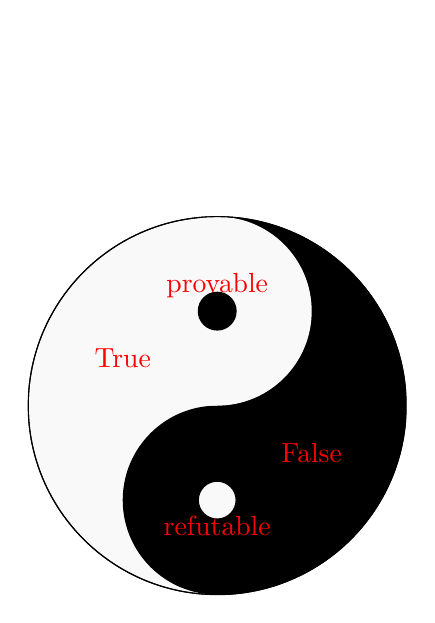
\begin{tikzpicture}[scale=.3]
	\begin{scope}
 \clip (0cm, -8cm) rectangle (8cm, 16cm);
 \draw[fill=black] (0cm, 0cm) circle (8cm);
	\end{scope}
	\begin{scope}
 \clip (0cm, -8cm) rectangle (-8cm, 16cm);
 \draw[fill=gray!5] (0cm, 0cm) circle (8cm);
	\end{scope}
 
 \fill[black] (0cm, -4cm) circle (4cm);
 \fill[gray!5] (0cm, 4cm) circle (4cm);
 
 \draw[] (0cm, 0cm) circle (8cm);

 \draw[fill=gray!5] (0,-4) circle (0.8cm);
 \draw[fill=black] (0,4) circle (0.8cm);

 \node at (-4cm, 2cm) {\textcolor{red}{True}};
 \node at (0cm, -5.1cm) {\textcolor{red}{refutable}};
 
 \node at (4cm, -2cm) {\textcolor{red}{False}};
 \node at (0cm, 5.1cm) {\textcolor{red}{provable}};
\end{tikzpicture}
\end{figure}
\end{minipage}}
\column{.45\textwidth}
	\begin{figure}
		\includegraphics[width=\textwidth,angle=0,origin=c]{img/einstein-godel}
	\end{figure}
\end{columns}
\end{frame}

\begin{frame}\frametitle{老子$\sideset{^\circledcirc}{^\circledcirc}{\operatorname{\hat{o}}}$}
\begin{itemize}
	\item 道,可道,非常道;名,可名,非常名。
	\item 无名,天地之始;有名,万物之母。
	\item 故常无,欲以观其妙;常有,欲以观其徼。
	\item 此两者,同出而异名,同谓之玄。
	\item 玄之又玄,众妙之门。
\end{itemize}
\begin{block}{}
	The theory that can be formulated can't be the ultimate theory. The formulated theory of categories evolves, and its projection on reality changes. The unformulatable ultimate theory is the truth of universe. The formulated theory is the basis to describe all the matter. In search of the unformulatable ultimate theory, we give meaning to life. Within the formulated theory, we study its limits. The gap between the formulatable and the unformulatable is a mystery. From the formulated to the unformulated and from the unformulated to the formulated is the gateway to all understanding.
\end{block}
\end{frame}

\begin{frame}\frametitle{G\"odel's First Incompleteness Theorem}
\setlength\abovedisplayskip{0pt}
\setlength\belowdisplayskip{0pt}
	\begin{theorem}[G\"odel's First Incompleteness Theorem]
		For any G\"odelian $\mathrm{T}\supset \mathrm{Q}$, $\operatorname{Cn}(\mathrm{T})\subsetneq \operatorname{Th}(\mathcal{N})$.
	\end{theorem}
	\begin{block}{G\"odel's First Incompleteness Theorem}
		\[F(x)\coloneqq \neg\Box x\]
		\[G=\text{\textcolor{yellow}{``I am not provable.''}}\]
		\[\mathrm{T}\vdash\operatorname{Con}_\mathrm{T}\to\neg\Box G\]
	\end{block}
\begin{proof}
$G\leftrightarrow\neg\Box G\implies\Box G\to\neg G\implies\Box(\Box G\to\neg G)\implies\Box G\to\Box\neg G\implies\Box G\to\Box(G\wedge\neg G)\implies\neg\Box\bot\to\neg\Box G$
\end{proof}
\begin{columns}
	\column{.27\textwidth}
	{\footnotesize For every record player, there are records that it can't play.\\(sympathetic vibration)}
	\column{.17\textwidth}
		\includegraphics[width=\textwidth]{img/record.png}
	\column{.51\textwidth}
	{\large We now know enough to know that\\ we will never know everything.}
\end{columns}
\end{frame}

\begin{frame}\frametitle{Tarski's Undefinability Theorem}
\begin{theorem}[Tarski's Undefinability Theorem]
	There is no definable predicate $B(x)$ in the language of arithmetic, such that $\mathcal{N}\vDash A\leftrightarrow B(\ulcorner A\urcorner)$.
\end{theorem}
	\begin{block}{}
		\[\text{suppose $\big\{\ulcorner A\urcorner:\mathcal{N}\vDash A\big\}$ is definable by $B(x)$.}\]
		\[F(x)\coloneqq \neg B(x)\]
		\[G=\text{\textcolor{yellow}{``I am not true.''}}\]
	\end{block}
\end{frame}

\begin{frame}\frametitle{Strength \& Limitation}
	\begin{quote}
		God plays dice both in quantum mechanics and in pure math. \par
		\hfill --- \textsl{Gregory Chaitin}
	\end{quote}
	\begin{quote}
		It is the duty of the human understanding to understand that there are things which it can't understand, and what those things are.\par
		\hfill --- \textsl{S{\o}ren Kierkegaard}
	\end{quote}
	\begin{quote}
		The only way of discovering the limits of the possible is to venture a little way past them into the impossible. \par
		\hfill --- \textsl{Arthur Charles Clarke}
	\end{quote}
\end{frame}

\begin{frame}\frametitle{}
\begin{figure}[H]
\includegraphics[width=\textwidth]{img/beyond-limits.jpg}
\end{figure}
\end{frame}

\begin{frame}\frametitle{Math-Matter-Mind (Penrose)}
\[
\begin{tikzcd}[column sep=huge, row sep=huge]
\boxed{Mathematical\atop{Structure\atop{\textcolor{red}{defined?}}}} \arrow[rr, bend right=10, "\text{defined by}" swap, marking] \arrow[ddr, bend right=10, "\text{model of}" swap, marking] \&\& \boxed{Computation\atop{\textcolor{red}{halting?}}} \arrow[ll, bend right=10, "\text{special case of}", marking] \arrow[ddl, bend right=10, "\text{theorem proving}", marking] \\
\& \\
\& \boxed{Formal\atop{System\atop{\textcolor{red}{decidable?}}}} \arrow[uul, bend right=10, "\text{decide}", marking] \arrow[uur, bend right=10, "\text{describe}" swap, marking]
\end{tikzcd}
\]
\end{frame}

\begin{frame}\frametitle{}
	\begin{columns}
		\column{0.53\textwidth}
			\includegraphics[width=\textwidth,angle=0,origin=c]{img/penrose-three-worlds.pdf}
		\column{0.51\textwidth}
\[
\begin{tikzcd}
\text{Mind} \arrow[rr,Rightarrow] \&\& \text{Math} \arrow[ddl,Rightarrow]\\
\&\\
\& \text{Matter} \arrow[uul,Rightarrow]
\end{tikzcd}
\]
\[
\begin{tikzcd}
\text{Mind} \&\& \text{Math} \\
\& \textcolor{red}{?} \arrow[dd, Rightarrow] \arrow[ul, Rightarrow] \arrow[ur, Rightarrow]\\
\&\\
\& \text{Matter}
\end{tikzcd}
\]
	\end{columns}
\end{frame}

\begin{frame}\frametitle{Deduction vs Induction}
	\begin{table}[H]\small
		\begin{center}
			\resizebox{.98\textwidth}{!}{
					\begin{minipage}{77ex}
\abovetabulinesep=1mm
\belowtabulinesep=1mm\begin{tabu}{l|rcl}
						\hline
							& \textbf{Induction} & $\mathbf{|}$ & \textbf{Deduction} \\ \hline
							Type of inference & generalization/prediction& $\Leftrightarrow$ & specialization/derivation \\
							Framework & probability axioms & $\widehat=$ & logical axioms \\ % better word for framework
							Assumptions & prior & $\widehat=$ & non-logical axioms \\ % postulates
							Inference rule & Bayes rule & $\widehat=$ & modus ponens \\
							Results & posterior & $\widehat=$ & theorems \\
							Universal scheme & Solomonoff probability & $\widehat=$ & $\mathrm{ZFC}$ \\
							Universal inference& universal induction & $\widehat=$ & universal theorem prover \\ 
							\hline
							Limitation & uncomputable (Turing) &
							$\widehat=$ & imcomplete (G\"odel)\\
							In practice & approximations &
							$\widehat=$ & semi-formal proofs\\
							Operation & computation &
							$\widehat=$ & proof\\
						\hline
						\end{tabu}
			\end{minipage}}
		\end{center}
	\end{table}
\end{frame}

\begin{frame}\frametitle{Logic vs Statistics}%\vspace{-1ex}
\begin{table}\centering
\begin{tabu}{p{.29\textwidth}|p{.29\textwidth}|p{.3\textwidth}}
\hline
\textbf{Field} & \textbf{Logical Approach} & \textbf{Statistical Approach}\\
\hline
Knowledge representation & First order logic & Graphical models\\
\hline
Automated reasoning & Satisfiability testing & Markov chain Monte Carlo\\
\hline
Machine learning & Inductive logic programming & Neural networks\\
\hline
Planning & Classical planning & Markov decision processes\\
\hline
Natural language processing & Definite clause grammars & Probabilistic context-free grammars\\
\hline
\end{tabu}
\end{table}
	\begin{table}
		\centering
		\begin{tabu}{c|c}
			\hline
			\large\textcolor{red}{Logic} &\large\textcolor{red}{Statistics}\\
			\hline
			rule-based &data-driven\\
			\hline
			rigour &possibility\\
			\hline
			knowable &black-box\\
			\hline
			simple \& perfect world &complex \& uncertain world\\
			\hline
			\Large\textcolor{red}{$\times$} &\Large\textcolor{red}{$\checkmark$}\\
			\hline
		\end{tabu}%\vspace{-1ex}\caption{How to unify?}
	\end{table}
\end{frame}

\begin{frame}\frametitle{Probability vs Logic}
\begin{figure}[H]
\includegraphics[width=\textwidth]{img/probability-logic.png}	
\end{figure}
\end{frame}

\begin{frame}\frametitle{Prediction with Expert Advice}
\begin{itemize}
	\item Assume that there is some large, possibly infinite, class of `experts' which make predictions.
	\item The aim is to observe how each of these experts perform and predicts asymptotically as well as the best expert in hindsight.
\end{itemize}

\[
\abovetabulinesep=1mm
\belowtabulinesep=1mm
	\begin{tabu}{l|cccc|ccc}
	\hline
	& \mbox{Expert}_1 & \mbox{Expert}_2 & \dots & \mbox{Expert}_n & \mathrm{PEA} & true & loss \\
	\hline
	\mbox{day}_1 & 0 & 0 & \dots & 0 & 0 & 1 & 1\\
	\mbox{day}_2 & 0 & 1 & \dots & 1 & 1 & 1 & 0\\
	\mbox{day}_3 & 1 & 0 & \dots & 1 & 1 & 0 & 1\\
	\dots & \dots & \dots & \dots & \dots & \dots & \dots & \dots \\
	\hline
	\mbox{day}_t & y_t^1 & y_t^2 & \dots & y_t^n & y_t^\mathrm{PEA} & x_t & |y_t^\mathrm{PEA}-x_t| \\
	\hline
	\end{tabu}
\]
\end{frame}

\begin{frame}\frametitle{Prediction with Expert Advice}
	\begin{itemize}
		\item Follow the (perturbed) leader.
		\item Predicts according to a majority vote by the ``good'' experts.
		\item Multiplicative Weights. --- take expert which performed best in past with high probability and others with smaller probability.
		\item Regularization. Choose the class of all computable experts, and penalize ``complex'' experts.
		\item Universal Portfolios.
	\end{itemize}
\end{frame}

\begin{frame}\frametitle{Universal Portfolios}
	\begin{itemize}
		\item the agent chooses a distribution $\mathbf{b}_t\in\Delta_n\coloneqq \left\{\mathbf{x}\in[0,1]^n:\|\mathbf{x}\|_1=1\right\}$ of wealth over $n$ goods.
		\item nature chooses returns $\mathbf{x}_t\in(\mathbb{R}^+)^n$, where \[(\mathbf{x}_t)_i=\frac{\text{price of good $i$ at end of $t$}}{\text{price of good $i$ at beginning of $t$}}\]
		\item the total wealth.
		$W_t(\mathbf{b},\mathbf{x})=W_1\prod\limits_{k=1}^t\mathbf{b}_k^\mathsf{T}(\mathbf{x}_{<k})\mathbf{x}_k$
		\item regret.
		$R_t\coloneqq \max\limits_{\mathbf{b}\in\Delta_n}\sum\limits_{k=1}^t\log \mathbf{b}_k^\mathsf{T}(\mathbf{x}_{<k})\mathbf{x}_k-\sum\limits_{k=1}^t\log \mathbf{b}_k^\mathsf{T}(\mathbf{x}_{<k})\mathbf{x}_k$
		\item universal portfolios.
		\begin{align*}
		\hat{\mathbf{b}}_1&\coloneqq \left(\tfrac{1}{n},\dots,\tfrac{1}{n}\right)\\
		\hat{\mathbf{b}}_{t+1}(\mathbf{x}_{1:t})&\coloneqq \frac{\int_{\Delta_n}\!\!\mathbf{b} W_t(\mathbf{b},\mathbf{x})\mathrm{d}\mathbf{b}}{\int_{\Delta_n}\!\!W_t(\mathbf{b},\mathbf{x})\mathrm{d}\mathbf{b}}
		\end{align*}
		\item Asymptotic Optimality.
		$\frac{1}{t}\log W_t(\hat{\mathbf{b}},\mathbf{x})\xrightarrow{t\to\infty}\frac{1}{t}\log \max\limits_{\mathbf{b}\in\Delta_n}W_t(\mathbf{b},\mathbf{x})$
	\end{itemize}
\end{frame}

%--------------------------%
\subsection{Algorithmic Randomness}
%--------------------------%

\begin{frame}\frametitle{The Paradox of Randomness}
\begin{itemize}
	\item A random bit-string should be ``typical'': it should not stand out from the crowd of other bit-strings.
	\item Assume that there is a precise way to distinguish between ``random bit-strings'' and bit-strings which are ``non-random''.
	\item Can the adopted \textbf{criterion} be consistent?
	\item choose the first bit-string that the criterion asserts it is random. This particular bit-string is
	\begin{quote}
		\begin{center}
			``the first bit-string satisfying the property of being random''
		\end{center}
	\end{quote}
	a property making it atypical, so non-random!
\end{itemize}
\end{frame}

\begin{frame}\frametitle{Randomness}
\begin{description}[short label,long label]
	\item[\textcolor{green}{Typicalness}] \textcolor{yellow}{The statistician's approach:} A random sequence is the typical outcome of a random variable. Random sequences should not have effectively rare distinguishing properties.
	\item[\textcolor{green}{Incompressibility}] \textcolor{yellow}{The coder's approach:} Rare patterns can be used to compress information. Random sequences should not be effectively described by a significantly shorter description than their literal representation.
	\item[\textcolor{green}{Unpredictability}] \textcolor{yellow}{The gambler's approach:} A betting strategy can exploit rare patterns. Random sequences should be unpyellowictable. No effective martingale can make an infinite amount betting on the bits.
\end{description}
\end{frame}

\begin{frame}\frametitle{The Statistician's Approach}
\begin{itemize}
	\item A random sequence should be absolutely normal.
	\item If you select a subsequence, then it should satisfy the law of large numbers, the law of the iterated logarithm\dots
	\item But what selection functions should be allowed? Computable?
	\item Martin-L\"of: we can effectively test whether a particular infinite sequence does not satisfy a particular law of randomness by effectively testing whether the law is violated on increasingly long initial segments. We should consider the intersection of all sets of measure one with recursively enumerable complements. (Such a complement set is expressed as the union of a recursively enumerable set of cylinders).
\end{itemize}
\end{frame}

\begin{frame}\frametitle{Cantor Space $2^\omega$}
\begin{itemize}
	\item For $x\in 2^{<\omega}$, the cylinder set $\Gamma_x\coloneqq \{y\in 2^\omega: x\prec y\}$ is the basic open set. It corresponds to the interval $[0.x,0.x+2^{-\ell(x)})$.
	\item For $A\subset 2^{<\omega}$, the open set generated by $A$ is $\Gamma_A\coloneqq \bigcup\limits_{x\in A}\Gamma_x$.
	\item The Lebesgue measure $\mu(\Gamma_x)\coloneqq 2^{-\ell(x)}$, $\mu(x)\coloneqq \mu(\Gamma_x)$.
	\item The outer measure of $C\subset 2^\omega$ is $\mu^*(C)\coloneqq \inf\left\{\sum\limits_{x\in A}2^{-\ell(x)}: C\subset\Gamma_A\right\}$.
	\item The inner measure of $C$ is $\mu_*(C)\coloneqq 1-\mu^*(2^\omega\setminus C)$.
	\item If $C$ is measurable, then $\mu^*(C)=\mu_*(C)$.
	\item $A\subset 2^\omega$ has measure $0$ iff there is a sequence $\{V_n\}_{n\in\omega}$ of open sets s.t. $A\subset\bigcap\limits_{n\in\omega}V_n$ and $\lim\limits_{n\to\infty}\mu(V_n)=0$.
\end{itemize}
\end{frame}

\begin{frame}\frametitle{An analogy: airport terrorist testing$\sideset{^\circledcirc}{^\circledcirc}{\operatorname{\hat{o}}}$}
\begin{itemize}
	\item Null hypothesis: a passenger is not a terrorist.
	\item Tests:
	\begin{itemize}
		\item Passport checking
		\item Blacklist checking
		\item Baggage scanning
		\item Body Scanner
		\item Officials talk to you
	\end{itemize}
	\item Every time you pass one test, our level of confidence in the null hypothesis increases.
	\item If you fail any test, they arrest you.
	\item If you pass all possible tests, then with ``high confidence'', the null hypothesis holds.
\end{itemize}
\end{frame}

\begin{frame}\frametitle{History --- Mises-Wald-Church}
\begin{itemize}
\item In 1919, von Mises proposed the following two conditions for an infinite random sequence $x\in 2^\omega$:
\begin{enumerate}
	\item The limiting frequency $\lim\limits_{n\to\infty}\frac{\sum_{i=1}^n x_i}{n}$ exists.
	\item The limiting frequency persists for any subsequence selected by an admissible place-selection rule.
\end{enumerate}
\item What is an admissible place-selection rule?
\item If you allow any partial function to be admissible, then there is no random sequence.
\item Ward: if we allow only countably many functions, then von Mises sequences exist.
\item Church: let's use computable functions.
\item Ville: There exist sequences that satisfy the Mises-Wald-Church definition of randomness, with limiting frequency of ones of $\frac{1}{2}$, but nonetheless have the property
\[\forall n: \frac{\sum_{i=1}^nx_i}{n}\geq\frac{1}{2}\]
\end{itemize}
\end{frame}

\begin{frame}\frametitle{Nested Critical Regions}
Instead of stability under place-selection rules, Martin-L\"of's fundamental property is passing effective statistical tests.
\begin{figure}[H]
\includegraphics[height=.42\textwidth]{img/martin-lof.jpeg}
\includegraphics[height=.42\textwidth]{img/nesting-doll.jpg}
\end{figure}
\[V_1\supset V_2\supset V_3\supset\dots\]
As the critical regions become smaller, significance level increases.
\end{frame}

\begin{frame}\frametitle{Martin-L\"of Randomness}
\setlength\abovedisplayskip{0pt}
\setlength\belowdisplayskip{0pt}
\begin{definition}[Martin-L\"of Randomness]
\begin{itemize}
	\item A total lower semicomputable function $\delta: 2^{<\omega}\to\omega$ is a Martin-Löf test iff $\forall n:\mu(V_n)\leq 2^{-n}$, where $V_n\coloneqq \{x:\delta(x)\geq n\}$.
	\item $x\in 2^\omega$ is ML-random iff for every ML-test $\delta$, $\sup_n\delta(x_{1:n})<\infty$.
\end{itemize}
\end{definition}
\[\delta(x)<\infty\iff x\notin\bigcap\limits_{n=1}^\infty V_n\]
\begin{definition}[Martin-L\"of Randomness]
\begin{itemize}
	\item A Martin-Löf test is a c.e. set $V\subset\mathbb{N}\times 2^{<\infty}$ s.t. for $V_n\coloneqq\left\{x\in 2^{<\infty}: \langle n,x\rangle\in V\right\}$,
	\[\mu(V_n)\leq 2^{-n}\]
	\item $x\in 2^\omega$ is ML-random iff for every ML-test $V$,
	\[x\notin\bigcap\limits_{n=1}^\infty V_n\]
\end{itemize}
\end{definition}
\end{frame}

\begin{frame}\frametitle{Martin-L\"of Randomness}
\setlength\abovedisplayskip{0pt}
\setlength\belowdisplayskip{0pt}
\begin{definition}[Universal Martin-L\"of Test]
A ML-test $\delta_0$ is \emph{universal} iff for every ML-test $\delta$, $\exists c\forall x:\delta_0(x)\geq\delta(x)-c$.
\end{definition}
A ML-test $\{U_n\}_{n\in\omega}$ is \emph{universal} iff for every ML-test $\{V_n\}_{n\in\omega}$, $\bigcap\limits_{n\in\omega}U_n\supset\bigcap\limits_{n\in\omega}V_n$.
\begin{center}
\fbox{$\delta(x)\coloneqq \ell(x)-K(x\mid\ell(x))$ is a universal ML-test.}
\end{center}
\[R_b\coloneqq \big\{x\in 2^\omega:\exists n\big(K(x_{1:n})<n-b\big)\big\}\]
\begin{center}
\fbox{$\{R_b\}_{b\in\omega}$ is a universal ML-test.}
\end{center}
\begin{theorem}[Schnorr 1973]
A sequence $x\in 2^\omega$ is ML-random iff it is $1$-random.
\end{theorem}
\end{frame}

\begin{frame}\frametitle{The Gambler's Approach}
\begin{itemize}
	\item A martingale is a function $d: 2^{<\omega}\to[0,\infty)$ s.t. for every $\sigma\in 2^{<\omega}$
	\[d(\sigma)=\frac{d(\sigma0)+d(\sigma1)}{2}\]
	\item A supermartingale is a function $d: 2^{<\omega}\to[0,\infty)$ s.t. for every $\sigma\in 2^{<\omega}$
	\[d(\sigma)\geq\frac{d(\sigma0)+d(\sigma1)}{2}\]
	\item A (super)martingale $d$ succeeds on $x\in 2^\omega$ iff $\limsup\limits_{n\to\infty}d(x_{1:n})=\infty$.
\end{itemize}
\begin{theorem}
A sequence $x\in 2^\omega$ is ML-random iff no c.e. (super)martingale succeeds on it.
\end{theorem}
\end{frame}

\begin{frame}\frametitle{The Coder's Approach}
\setlength\abovedisplayskip{0pt}
\setlength\belowdisplayskip{0pt}
\begin{columns}
\column{.39\textwidth}
\begin{definition}[$1$-Randomness]
$x\in 2^\omega$ is $1$-random iff
\[\exists c\forall n: K(x_{1:n})\geq n-c\]
\end{definition}
\column{.62\textwidth}
\begin{theorem}
The following are equivalent.
\begin{itemize}
	\item $x\in 2^\omega$ is ML-random.
	\item No c.e. (super)martingale succeeds on it.
	\item $\exists c\forall n: K(x_{1:n})\geq n-c$
	\item $\forall n: Km(x_{1:n})\eqa n$
	\item $\lim\limits_{n\to\infty}K(x_{1:n})-n=\infty$
	\item $\sum\limits_{n=1}^\infty 2^{n-K(x_{1:n})}<\infty$
	\item $\sup_n 2^{n-K(x_{1:n})}<\infty$
	\item $C(x_{1:n})\geqa n-K(n)$
	\item $C(x_{1:n})\geqa n-f(n)$ for every computable $f$ s.t. $\sum\limits_{n=1}^\infty 2^{-f(n)}<\infty$.
\end{itemize}
\end{theorem}
\end{columns}
\end{frame}

\begin{frame}\frametitle{}
\begin{definition}[Solovay Reducibility]
Let $a_n\to\alpha$ and $b_n\to\beta$ be two computable strictly increasing sequences of rationals converging to lower semicomputable reals $\alpha$ and $\beta$. We say that $\alpha\leq_S\beta$ iff there is a constant $c$ and a total computable function $f$ s.t. $\forall n:\alpha-a_{f(n)}\leq c(\beta-b_n)$.
\end{definition}
\begin{theorem}
For lower semicomputable reals $\alpha$, the following are equivalent.
\begin{itemize}
	\item $\alpha$ is $1$-random
	\item $\alpha\geq_S\beta$ for all lower semicomputable reals $\beta$.
	\item $\alpha\geq_S\Omega$
	\item $K(\alpha_{1:n})\geqa K(\beta_{1:n})$ for all lower simicomputable reals $\beta$.
	\item $K(\alpha_{1:n})\geqa K(\Omega_{1:n})$
	\item $K(\alpha_{1:n})\eqa K(\Omega_{1:n})$
	\item $\alpha=\Omega_U\coloneqq \sum\limits_{p:U(p)\downarrow}2^{-\ell(p)}$ for some universal prefix Turing machine $U$.
\end{itemize}
\end{theorem}
\end{frame}

\begin{frame}\frametitle{$\mu/\xi$-randomness}
\begin{definition}[$\mu/\xi$-randomness]
\begin{itemize}
	\item A sequence $x\in 2^\omega$ is $\mu/\xi$-random iff $\exists c\forall n: \xi(x_{1:n})\leq c\cdot\mu(x_{1:n})$.
	\item A sequence $x\in 2^\omega$ is $\mu$-ML-random iff $\exists c\forall n: M(x_{1:n})\leq c\cdot\mu(x_{1:n})$.
\end{itemize}
\end{definition}
\begin{block}{}
\begin{itemize}
\item $x_{1:\infty}$ is $\mu$-ML-random iff $\sup_n\delta(x_{1:n}\mid\mu)<\infty$, where
\[\delta(x\mid\mu)\coloneqq \log\frac{M(x)}{\mu(x)}\]
\item For a computable $\mu$, $x_{1:\infty}$ is $\mu$-ML-random iff
\[\forall n: Km(x_{1:n})\eqa-\log\mu(x_{1:n})\]
\end{itemize}	
\end{block}
\end{frame}

\begin{frame}\frametitle{Properties of ML-Random Sequences}
\begin{itemize}
\item Special case of $\mu$ being a fair coin, i.e. $\mu(x_{1:n}) = 2^{-n}$, then
\[\mbox{$x_{1:\infty}$ is random} \iff Km(x_{1:n})\eqa n,\;\; \mbox{i.e. iff $x_{1:n}$ is incompressible.}\]
\item For general $\mu$, $-\log\mu(x_{1:n})$ is the length of the Arithmetic code of $x_{1:n}$, hence
\[\mbox{$x_{1:\infty}$ is $\mu$-random} \iff \mbox{ the Arithmetic code is optimal.}\]
\item One can show that a $\mu$-random sequence $x_{1:\infty}$ passes all thinkable effective randomness tests, e.g. the law of large numbers, the law of the iterated logarithm, etc.
\item In particular, the set of all $\mu$-random sequences has $\mu$-measure $1$.
\end{itemize}
\end{frame}

\begin{frame}\frametitle{Randomness, Triviality}
\begin{itemize}
\item $A\subset\mathbb{N}$ is \emph{low} iff $A'\leq_T\emptyset'$, and $A$ is \emph{high} iff $\emptyset''\leq_T A'$.
\item $A$ is \emph{low for ML-randomness} iff each ML-random set is already ML-random relative to $A$.
\item $A$ is \emph{low for $K$} iff $\exists c\forall x: K(x)\leq K^A(x)+c$.
\item $x\in 2^\omega$ is \emph{$K$-trivial} iff $\exists c\forall n: K(x_{1:n})\leq K(n)+c$.
\end{itemize}
\begin{theorem}
$A$ is $K$-trivial $\iff$ $A$ is low for ML-randomness $\iff A$ is low for $K$.
\end{theorem}
Some sequences are $K$-trivial but not computable.\\
Neither randoms, nor $K$-trivials, are deep.
\end{frame}

\begin{frame}\frametitle{Effective Hausdorff dimension can be interpreted as a degree of incompressibility}
\begin{definition}
A set $A\subset 2^\omega$ has \emph{effective $d$-dimensional Hausdorff measure $0$}, $H^d(A)=0$, iff there exists a c.e. set $V\subset\mathbb{N}\times 2^{<\omega}$ s.t., for $V_n\coloneqq\left\{x\in 2^{<\omega}: \langle n,x\rangle\in V\right\}$
\[A\subset\bigcup\limits_{x\in V_n}\Gamma_x\quad\mbox{ and }\quad \sum\limits_{x\in V_n}\mu(\Gamma_x)^d=\sum\limits_{x\in V_n}2^{-\ell(x)d}\leq 2^{-n}\]
\end{definition}
\begin{definition}[Effective Hausdorff Dimension]
The \emph{effective Hausdorff dimension} of $A\subset 2^\omega$ is defined as
\[\dim_H^1(A)\coloneqq\inf\left\{d\geq 0: H^d(A)=0\right\}\]
\end{definition}
\begin{theorem}
\[\dim_H^1(x)=\liminf\limits_{n\to\infty}\frac{K(x_{1:n})}{n}\]	
\end{theorem}
\end{frame}

%--------------------------%
\subsection{Effective Complexity}
%--------------------------%

\begin{frame}\frametitle{Mandelbrot Set --- complex structure from simple rule}
\vspace*{-2ex}
\begin{figure}[H]
\includegraphics[width=.32\textwidth]{img/mandelbrot1.jpeg}
\includegraphics[width=.32\textwidth]{img/mandelbrot2.jpeg}
\includegraphics[width=.32\textwidth]{img/mandelbrot3.jpeg}
\includegraphics[width=.32\textwidth]{img/mandelbrot4.jpeg}
\includegraphics[width=.32\textwidth]{img/mandelbrot5.jpeg}
\includegraphics[width=.32\textwidth]{img/mandelbrot6.jpeg}
\end{figure}
\[z\mapsto z^2+c\]
\end{frame}

\begin{frame}\frametitle{What is Complexity?}
\begin{enumerate}
	\item How hard is it to describe?
	\begin{itemize}
		\item Shannon Entropy
		\item Kolmogorov Complexity
		\item Minimum Description Length
		\item Statistical Complexity: the minimum amount of information about the past behavior of a system that is needed to optimally predict the statistical behavior of the system in the future.
		\item Fisher Information
		\item Renyi Entropy
	\end{itemize}
	\item How hard is it to create?
	\begin{itemize}
		\item Computational Complexity
		\item Logical Depth
		\item Thermodynamic Depth: the Shannon entropy of trajectories leading to the current state.
	\end{itemize}
	\item What is its degree of organization?
	\begin{itemize}
		\item Effective Complexity / Sophistication
		\item Fractal Dimension
		\item Stochastic Complexity
		\item Hierarchical Complexity
		\item Channel Capacity
	\end{itemize}
\end{enumerate}
\end{frame}

\begin{frame}\frametitle{Features of Complex Systems}
\begin{enumerate}
	\item Numerosity: involve many interactions among many components.
	\item Disorder and diversity: the interactions in a complex system are not coordinated or controlled centrally, and the components may differ.
	\item Feedback: the interactions are iterated so that there is feedback from previous interactions relevant to the system's emergent dynamics.
	\item Non-equilibrium: complex systems are open to the environment and are often driven by something external.
	\item Spontaneous order and self-organisation: exhibit structure and order that arises out of the interactions among their parts.
	\item Nonlinearity: exhibit nonlinear dependence on parameters.
	\item Robustness: the structure and function is stable under relevant perturbations.
	\item Nested structure and modularity: there may be multiple scales of structure, clustering and specialisation of function in complex systems.
	\item History and memory: often require a very long history to exist.
	\item Adaptive behaviour: often able to modify their behaviour depending on the state of the environment and the predictions they make about it.
\end{enumerate}	
\end{frame}

\begin{frame}\frametitle{}
There are various kinds of invariance and forms of universal behaviour in complex systems.
\begin{figure}[H]
\includegraphics[width=.7\textwidth]{img/metabolic-rate.jpg}
\end{figure}
\begin{itemize}
	\item $B\propto M^{3/4}$ whole-organism metabolic rate (B) scales as $3/4$ power of body mass (M)
\end{itemize}
\end{frame}

\begin{frame}\frametitle{}
\begin{figure}[H]
\includegraphics[width=\textwidth]{img/heart-rate.png}	
\end{figure}
\begin{itemize}
	\item $R\propto M^{-1/4}$ heart rate (R) scales as $-1/4$ power of body mass (M)
	\item metabolic rate sets the pace of life
	\item small animals live fast and die young
\end{itemize}
\end{frame}

\begin{frame}\frametitle{Complexity \& Scale}
\begin{itemize}
	\item Are cities and companies just very large organisms satisfying the laws of biology?
	\item Why do all companies die whereas almost all cities survive?
\end{itemize}
\begin{itemize}
	\item In biology, the network principles underlying economies of scale and \textcolor{red}{sublinear scaling} have two profound consequences. They constrain the pace of life --- big animals live longer, evolve more slowly, and have slower heart rates --- and limit growth.
	\item Cities and economies are driven by social interactions whose feedback mechanisms lead to the opposite behavior. The pace of life increases with population size. Moreover, the social network dynamic underlying \textcolor{red}{superlinear scaling} leads to open-ended growth. Continuous adaptation, not equilibrium, is the rule.
\end{itemize}
\[
\begin{matrix}
	\text{Incoming Metabolised Energy}\\
	\Downarrow\\
	\text{Maintenance of existing cells}\\
	+\\
	\text{Growth of new cells}
\end{matrix}
\]
\end{frame}

\begin{frame}\frametitle{Logical Depth}
\begin{definition}[Logical Depth]
The logical depth of $x$ at a significance level $b$ is
\[\operatorname{depth}_b(x)\coloneqq \min\left\{t: U^t(p)=x\;\;\&\;\;\ell(p)-K(x)\leq b\right\}\]
\end{definition}
We say $x$ is \emph{shallow} iff $\operatorname{depth}_b(x)\leqa\ell(x)$.

\begin{itemize}
	\item Crystal is shallow.
	\item Gas is also shallow.
	\item A math book is deep.
	\item Life is deep.
	\begin{quote}
		``If people do not believe that mathematics is simple, it is only because they do not realize how complicated life is.''\par \hfill --- \textsl{John von Neumann}
	\end{quote}
	\item $\chi_{1:\infty}$ is deep, where $\chi_i\coloneqq \llbracket\varphi_i(i)\downarrow\rrbracket$.
	\item $\Omega$ is shallow.
\end{itemize}
\end{frame}

\begin{frame}\frametitle{Effective Complexity}
	\resizebox{\textwidth}{!}{
	\begin{minipage}{\textwidth}
				\begin{align*}
				\delta(x\mid A)&\coloneqq \log |A|-K(x\mid A) &\text{[randomness deficiency]}\\
				\delta(x\mid \mu)&\coloneqq \log\dfrac{M(x)}{\mu(x)} &\text{[$\mu$-randomness deficiency]}\\
				\beta_x(k)&\coloneqq \min\limits_A\{\delta(x\mid A): x\in A\;\;\&\;\;K(A)\leq k\} &\text{[Best-Fit]}\\
				h_x(k)&\coloneqq \min\limits_A\{\log |A|: x\in A\;\;\&\;\;K(A)\leq k\} &\text{[Kolmogorov structure function / ML]}\\
				h_x(k)&\coloneqq \min\limits_\mu\{-\log \mu(x): K(\mu)\leq k\} &\text{[Kolmogorov structure function / ML]}\\
				A^*(x)&\coloneqq \iota A\Big[x\in A\;\;\&\;\;K(A)=\mu k\big[k+h_x(k)\eqa K(x)\big]\Big]&\text{[Kolmogorov minimal sufficient statistic]}\\
				\lambda_x(k)&\coloneqq \min\limits_A\left\{K(A)+\log |A|: x\in A\;\;\&\;\;K(A)\leq k\right\} &\text{[MDL]}\\
				\lambda_x(k)&\coloneqq \min\limits_\mu\{K(\mu)-\log\mu(x): K(\mu)\leq k\} &\text{[MDL]}\\
				\Delta(x\mid A)&\coloneqq K(A)+\log |A|-K(x) &\text{[discrepancy]}\\
				\operatorname{soph_c}(x)&\coloneqq \min\limits_A\{K(A):\Delta(x\mid A)<c\} &\text{[sophistication]}\\
				\operatorname{csoph}(x)&\coloneqq \min\limits_A\{K(A)+\Delta(x\mid A)\} &\text{[coarse sophistication]}\\
				\Sigma(\mu)&\coloneqq K(\mu)+H(\mu) &\text{[total information]}\\
				\mathcal{E}_{\delta,\Delta}(x\mid \mathcal{M})&\coloneqq \min\limits_{\mu\in\mathcal{M}}\left\{K(\mu):\Sigma(\mu)-K(x)\leq\Delta\;\;\&\;\;\mu(x)\geq 2^{-H(\mu)(1+\delta)}\right\} &\text{[effective complexity]}\\
				\mathcal{E}_\delta(x\mid \mathcal{M})&\coloneqq \min\limits_{\mu\in\mathcal{M}}\left\{K(\mu)+\Sigma(\mu)-K(x): \mu(x)\geq 2^{-H(\mu)(1+\delta)}\right\} &\text{[coarse effective complexity]}
				\end{align*}
	\end{minipage}}
\end{frame}

\begin{frame}\frametitle{Simon's Ant}
\begin{figure}[H]
\includegraphics[width=.4\textwidth]{img/ant.jpeg}
\includegraphics[width=.55\textwidth]{img/ant-environment.png}
\end{figure}
\begin{itemize}
	\item An ant, viewed as a behaving system, is quite simple. The apparent complexity of its behavior over time is largely a reflection of the complexity of the environment in which it finds itself.
	\item The mind is one blade in a pair of scissors, the structure of the environment is the other. To understand behaviour, one has to consider both --- and, in particular, how they fit.
\end{itemize}
\end{frame}

\begin{frame}\frametitle{}
\begin{columns}
\column{.5\textwidth}
\begin{figure}[H]
\includegraphics[width=\textwidth]{img/structure-function.pdf}
\end{figure}
\column{.5\textwidth}
\begin{figure}[H]
\includegraphics[width=\textwidth]{img/sufficient-statistic.pdf}
\end{figure}
\end{columns}
\end{frame}

\begin{frame}\frametitle{}
\begin{theorem}
For $x$ and $k$,
\[\lambda_x(k)\leq h_x(k)+k\leqa\lambda_x(k)+K(k)\]
For $k$ with $0\leq k\leq K(x)-O(\log\ell(x))$,
\[\beta_x(k)+K(x)\leqa\lambda_x(k)\]
\[\lambda_x(k+O(\log \ell(x)))\leq\beta_x(k)+K(x)\]
\end{theorem}
In other words, the equality
\[\beta_x(k)+K(x)=\lambda_x(k)=h_x(k)+k\]
holds within logarithmic additive terms in argument and value.
\end{frame}

\begin{frame}\frametitle{Sophistication and Computational Depth}
\begin{theorem}
\[\operatorname{csoph}(x)=\min\limits_c\{\operatorname{soph_c}(x)+c\}\]
\end{theorem}
\begin{align*}
K^t(x)&\coloneqq \min\limits_p\{\ell(p): U^t(p)=x\}\tag{\text{\footnotesize Time-bounded Kolmogorov Complexity}}\\
\operatorname{depth^t}(x)&\coloneqq K^t(x)-K(x)\tag{\text{\footnotesize Basic Computational Depth}}\\
\operatorname{depth_{BB}}(x)&\coloneqq \min\limits_t\{\operatorname{depth^t}(x)+K(t)\}\tag{\text{\footnotesize Busy Beaver Computational Depth}}
\end{align*}
\begin{theorem}
\[|\operatorname{csoph}(x)-\operatorname{depth_{BB}}(x)|\leq O(\log \ell(x))\]
\end{theorem}
\end{frame}

\begin{frame}\frametitle{Zurek's Physical Entropy}
\setlength\abovedisplayskip{0pt}
\setlength\belowdisplayskip{0pt}
\begin{definition}[Physical Entropy]
Physical entropy $S(d)$ of a microstate $d$ is the sum of the conditional Shannon entropy $H_d\coloneqq -\sum\limits_k P(k\mid d)\log P(k\mid d)$ and of the Kolmogorov Complexity $K(d)$.
\[S(d)\coloneqq H_d+K(d)\]
\end{definition}
\begin{figure}[H]
	\begin{center}
		\includegraphics[width=0.7\textwidth,angle=0,origin=c]{img/physical-entropy.pdf}\caption{random vs regular microstate}
	\end{center}
\end{figure}
\end{frame}

\begin{frame}\frametitle{Maxwell's Demon \& Landauer's Principle}
\begin{columns}
\column{.75\textwidth}
\begin{figure}[H]
\includegraphics[width=\textwidth]{img/maxwell-demon}\caption{The demon turns entropy into information, the information-erasure operation turns information into entropy. In the course of ideal measurement on an equilibrium ensemble, the decrease of the entropy must be compensated by the increase of the size of the minimal record, and vice versa. $\Delta H\approx-\langle\Delta K\rangle$.}
\end{figure}
\column{.25\textwidth}
\begin{figure}[H]
\includegraphics[width=\textwidth]{img/books-burning}\caption{\tiny Destroying information generates heat}
\end{figure}
\end{columns}
\end{frame}

\begin{frame}\frametitle{Landauer's Principle}
\begin{itemize}
	\item Landauer's Principle: Logically irreversible computation costs energy. Erasing $1$ bit of information dissipates at least $kT\ln2$ of heat into the environment.
	\item The ultimate thermodynamic cost of erasing $x$ is reached by:
	\begin{itemize}
		\item reversibly compress $x$ to $x^*$,
		\item then erase $x^*$. Cost $\sim K(x)$ bits.
	\end{itemize}
	\item The longer you compute, the less heat dissipation.
\end{itemize}
\end{frame}

\begin{frame}\frametitle{G\'acs' Algorithmic Entropy}
\setlength\abovedisplayskip{0pt}
\setlength\belowdisplayskip{0pt}
\begin{definition}[Algorithmic Entropy]
\begin{itemize}
	\item \emph{coarse-grained algorithmic entropy} of a cell $\Gamma$ with respect to $\mu$
	\[H_\mu(\Gamma)\coloneqq \log\mu(\Gamma)+K(\Gamma\mid \mu)\]
	\item \emph{fine-grained algorithmic entropy} of $x\in 2^\omega$ with respect to $\mu$
	\[H_\mu(x)\coloneqq \inf_n\big\{\log\mu(x_{1:n})+K(x_{1:n}\mid \mu)\big\}\]
\end{itemize}
\end{definition}
\begin{itemize}
	\item $-H_\mu(x)$ is a universal ML-test: $x$ is $\mu$-ML-random iff $H_\mu(x)>-\infty$.
	\item The fine-grained algorithmic entropy of a microstate can be approximated by the coarse-grained algorithmic entropies of successively smaller cells containing it.
	\[H_\mu(x)=\inf_n\big\{H_\mu(\Gamma_{x_{1:n}})\big\}\]
\end{itemize}
\end{frame}

\begin{frame}\frametitle{PageRank}
\begin{itemize}
	\item In a network with n nodes, assign all nodes the same initial PageRank, $1/n$.
	\item Choose a number of steps, $k$.
	\item Perform a sequence of $k$ updates to the PageRank values:
	\begin{itemize}
		\item[---] Basic PageRank Update Rule: Each page divides its current PageRank equally across its outgoing links and passes these equal shares to the pages it points to. (If a page has no outgoing links, it passes all its current PageRank to itself.) Each page updates its new PageRank to be the sum of the shares it receives.
		\item[---] Scaled PageRank Update Rule: First apply the Basic PageRank Update Rule. Then scale down all PageRank values by a factor of $s$. This means that the total PageRank in the network has shrunk from $1$ to $s$. We divide the residual $1-s$ units of PageRank equally over all nodes, giving $(1-s)/n$ to each.
	\end{itemize}
\end{itemize}	
\end{frame}

\begin{frame}\frametitle{PageRank}
\begin{columns}
\column{.45\textwidth}
\begin{figure}[H]
\includegraphics[width=\textwidth]{img/pagerank.pdf}		
\end{figure}
\column{.55\textwidth}
\[
\abovetabulinesep=1mm
\belowtabulinesep=1mm
\begin{tabu}{c|c|c|c|c|c|c|c|c}
\hline
k & A & B & C & D & E & F & G & H\\
\hline
0 & \frac{1}{8} & \frac{1}{8} & \frac{1}{8} & \frac{1}{8} & \frac{1}{8} & \frac{1}{8} & \frac{1}{8} & \frac{1}{8}\\
\hline
1 & \frac{1}{2} & \frac{1}{16} & \frac{1}{16} & \frac{1}{16} & \frac{1}{16} & \frac{1}{16} & \frac{1}{16} & \frac{1}{8}\\
\hline
2 & \frac{3}{16} & \frac{1}{4} & \frac{1}{4} & \frac{1}{32} & \frac{1}{32} & \frac{1}{32} & \frac{1}{32} & \frac{1}{16}\\
\hline
\vdots & \vdots & \vdots & \vdots & \vdots & \vdots & \vdots & \vdots & \vdots\\
\hline
\infty & \frac{4}{13} & \frac{2}{13} & \frac{2}{13} & \frac{1}{13} & \frac{1}{13} & \frac{1}{13} & \frac{1}{13} & \frac{1}{13}\\
\hline
\end{tabu}
\]
\end{columns}
\begin{itemize}
	\item Google's founding philosophy is that we don't know why this page is better than that one: If the statistics of incoming links say it is, that's good enough. No semantic or causal analysis is required. That's why Google can translate languages without actually ``knowing'' them.
\end{itemize}
\end{frame}

\begin{frame}\frametitle{\href{https://www.wired.com/2008/06/pb-theory/}{The End of Theory: The Data Deluge Makes the Scientific Method Obsolete \hfill --- \textsl{Chris Anderson}}}
\begin{itemize}
	\item All models are wrong, but some are useful.
	\item All models are wrong, and increasingly you can succeed without them.
	\item ``Correlation is enough''. We can stop looking for models. We can analyze the data without hypotheses about what it might show. We can throw the numbers into the biggest computing clusters the world has ever seen and let statistical algorithms find patterns where science cannot.
	\item The new availability of huge amounts of data, along with the statistical tools to crunch these numbers, offers a whole new way of understanding the world. Correlation supersedes causation, and science can advance even without coherent models, unified theories, or really any mechanistic explanation at all.
	\item There's no reason to cling to our old ways. It's time to ask: What can science learn from Google?
\end{itemize}
\end{frame}

\begin{frame}\frametitle{Ramsey in the Dining Room}
	\begin{problem}[Complete Disorder is Impossible!]
		\begin{itemize}
			\item How many people do you need to invite in a party in order to have that either at least $n$ of them are mutual strangers or at least $n$ of them are mutual acquaintances?
			\item How may we know that such number exists for any $n$?
		\end{itemize}
	\end{problem}
	\begin{columns}
		\column{0.3\textwidth}
			\begin{center}
				\begin{figure}
					\includegraphics[width=\textwidth,angle=0,origin=c]{img/pigeonhole.png}
				\end{figure}
			\end{center}
		\column{0.4\textwidth}
			\begin{center}\vspace{-7pt}
				\begin{tikzpicture}
				\node[
				regular polygon,
				regular polygon sides=5,
				minimum width=4.2cm,
				] (PG) {}
				(PG.corner 1) node (PG1) {1}
				(PG.corner 2) node (PG2) {2}
				(PG.corner 3) node (PG3) {3}
				(PG.corner 4) node (PG4) {4}
				(PG.corner 5) node (PG5) {5}
				;
				\foreach \S/\E in {2/1, 3/2, 4/3, 5/4, 1/5}{\draw[-,very thick,red] (PG\S) -- (PG\E);}
				\foreach \S/\E in {3/1, 1/4, 4/2, 2/5, 5/3}{\draw[-,very thick,green] (PG\S) -- (PG\E);}
				\end{tikzpicture}
			\end{center}
		\column{.3\textwidth}
		\begin{figure}
		\includegraphics[width=\textwidth]{img/beautiful-mind.jpg}
		\end{figure}
	\end{columns}
\end{frame}

\begin{frame}\frametitle{Complete Disorder is Impossible!}
	\begin{theorem}[Infinite Ramsey Theorem]
		If $(V,E)$ is a graph with infinitely many vertices, then it has an infinite clique or an infinite independent set.
	\end{theorem}
	\centerline{Infinite Ramsey Theorem $\xrightarrow{\textcolor{red}{\mbox{Compactness Theorem}}}$ Finite Ramsey Theorem}
	\begin{theorem}[Finite Ramsey Theorem]
		For every $m,n\geq 1$ there is an integer $R(m,n)$ s.t. any graph with at least $R(m,n)$ vertices has a clique with $m$ vertices or an independent set with $n$ vertices.
	\end{theorem}
	\vspace{-2ex}
	\[R(m,n)\leq R(m-1,n)+R(m,n-1)\]
	\[R(m,n)\leq \binom{m+n-2}{m-1}\]
\end{frame}

\begin{frame}\frametitle{Happy Ending Problem}
\vspace*{-2ex}
\begin{columns}
\column{.27\textwidth}
\begin{figure}[H]
\includegraphics[width=\textwidth]{img/happy-ending.png}
\end{figure}
\column{.7\textwidth}
\begin{block}{}
Any set of $5$ points in the plane in general position has a subset of $4$ points that form the vertices of a convex quadrilateral, where general position means that no two points coincide and no three points are collinear.
\end{block}
\end{columns}
\begin{theorem}[Erd\"os \& Szekeres 1935]
For $N\in\mathbb{N}$, any sufficiently large finite set of points in the plane in general position has a subset of $N$ points that form the vertices of a convex polygon.
\end{theorem}
Let $f(N)$ denote the minimum $M$ for which any set of $M$ points in general position must contain a convex $N$-gon. It is known that
\begin{itemize}
	\item $f(3)=3$
	\item $f(4)=5$
	\item $f(5)=9$
	\item $f(6)=17$
	\item $1+2^{N-2}\leq f(N)\leq 2^{N+o(N)}$
\end{itemize}
\end{frame}

\begin{frame}\frametitle{Complete Disorder is Impossible!}
	\begin{theorem}[Hales-Jewett Theorem]
		For every $k,n\in\mathbb{N}^+$, there is $d\in\mathbb{N}^+$ s.t. if the unit hypercubes in a $d$-dimensional hypercube $n^d$ are colored in $k$ colors, then there exists at least one row, column or diagonal of $n$ squares, all of the same color.
	\end{theorem}
	\begin{theorem}[van der Waerden Theorem]
		For every $k,m\in\mathbb{N}^+$, there is $n\in\mathbb{N}^+$ s.t. if the numbers from $1$ to $n$ are colored in $k$ colors, then there exists at least $m$ numbers in arithmetic progression, all of the same color.
	\end{theorem}
	\begin{theorem}[Green-Tao Theorem]
		A subset of prime numbers $A$ with $\limsup\limits_{n\to\infty}\frac{|A\cap[1,n]|}{\pi(n)}>0$ contains arbitrarily long arithmetic progressions, where $\pi(n)$ is the number of primes $\leq n$.
	\end{theorem}
\end{frame}

\begin{frame}\frametitle{Complete Disorder is Impossible!}
\setlength\abovedisplayskip{0pt}
	\begin{theorem}[Szemer\'edi Theorem]
		A set $A\subset\mathbb{N}$ with $\limsup\limits_{n\to\infty}{\frac {|A\cap [1,n]|}{n}}>0$ contains arbitrarily long arithmetic progressions.
	\end{theorem}
	\begin{theorem}[Furstenberg Multiple Recurrence Theorem]
		Let $(X,{\mathcal{B}},\mu,T)$ be a measure-preserving system and $A\in\mathcal{B}$ with $\mu(A) > 0$. Then,
		\[\forall k\in\mathbb{N}:\;\liminf\limits_{N\to\infty}\dfrac{1}{N}\sum\limits_{n=1}^N\mu\left(\bigcap\limits_{j=0}^k T^{-jn}A\right)>0\]
	\end{theorem}
	\[\text{Szemer\'edi Theorem}\iff\text{Furstenberg Multiple Recurrence Theorem}\]
\end{frame}

\begin{frame}\frametitle{Complete Disorder is Impossible!}
	\begin{theorem}[Poincar\'e Recurrence Theorem]
		Let $(X,{\mathcal{B}},\mu,T)$ be a measure-preserving system and $A\in\mathcal{B}$ with $\mu(A) > 0$. Then almost every $x\in A$ returns infinitely often to $A$.
		\[
		\mu\left(\{x\in A: \exists N\forall n>N: T^n x\notin A\}\right)=0
		\]
	\end{theorem}
	\begin{lemma}[Kac's Lemma]
		Let $(X,{\mathcal{B}},\mu,T)$ be a measure-preserving system and $A\in\mathcal{B}$ with $\mu(A) > 0$. Then the recurrence time $\tau_A(x)\coloneqq \min\left\{k\geq 1: T^k x\in A\right\}$ satisfies
		\[\int_A\!\tau_A(x)\mathrm{d}\mu(x)=1\]
		Equivalently, the mean recurrence time $\left\langle \tau_A\right\rangle\coloneqq \frac{1}{\mu(A)}\int_A\!\tau_A(x)\mathrm{d}\mu(x)=\frac{1}{\mu(A)}$.
	\end{lemma}
\end{frame}

\begin{frame}\frametitle{Correlation Supersedes Causation?}
	\begin{itemize}
		\item The average recurrence time to a subset $A$ in Poincar\'e recurrence theorem is the inverse of the probability of $A$. The probability decrease exponentially with the size (dimension) of the phase space (observables and parameters) and the recurrence time increases exponentially with that size. One can't reliably predict by ``analogy'' with the past, even in deterministic systems, chaotic or not.
		\item Given any arbitrary correlation on sets of data, there exists a large enough number such that any data set larger than that size realizes that type of correlation. Every large set of numbers, points or objects necessarily contains a highly regular pattern.
		\item There is no true randomness. Randomness means unpredictability with respect to some fixed theory.
	\end{itemize}
\end{frame}

\begin{frame}\frametitle{\href{https://www.cs.auckland.ac.nz/~cristian/crispapers/fos2016.pdf}{Correlation Supersedes Causation?}}\vspace{-1ex}
	\begin{itemize}
		\item How to distinguish correlation from causation?
		\item How to distinguish content-correlations from Ramsey-type correlations?
		\item Ramsey-type correlations appear in all
		large enough databases.
		\item A correlation is \emph{spurious} iff it appears in a ``randomly'' generated database.
		\item How ``large'' is the set of spurious correlations?
		\item Most strings are algorithmically random. 
		\[P\left(\Big\{x\in\mathcal{X}^n: \frac{K(x)}{n}<1-\delta\Big\}\right)<2^{-\delta n}\]
		\item Most correlations are spurious.
		\item It may be the case that our part of the universe is an oasis of regularity in a maximally random universe.
	\end{itemize}\vspace{-1ex}
	\begin{block}{Complete Disorder is Impossible!}
		For sufficiently large $n$ and any $x\in\mathcal{X}^n$, if $C(x)\geq n-\delta(n)$, then each block of length $\log n-\log\log n-\log(\delta(n)+\log n)-O(1)$ occurs at least once in $x$.
	\end{block}
\end{frame}

\begin{frame}\frametitle{Determinism, Indeterminism, Randomness and Free Will}
\begin{enumerate}
	\item If our actions are caused by chance we lack control.
	\item randomness, the operation of mere chance, clearly excludes control.
\end{enumerate}
Does randomness conflict with free will?
\begin{itemize}
	\item There is a \textcolor{red}{process conception of randomness} based on which random actions are chancy actions. (IT)
	\item There is a \textcolor{red}{product conception of randomness} based on which random happenings are lacking any discernible or explicable pattern. (AIT)
\end{itemize}
\begin{itemize}
	\item Is indeterminism necessary for free will?
	\item Is indeterminism necessary for randomness? No. The halting probability $\Omega_U$ is Martin-L\"of random, but \textbf{determined} by $U$.
	\item Is randomness necessary for indeterminism? No. There are automata that work in non-deterministic ways without use of randomness.
	\item Indeterminism and randomness do not imply each other.
	\item To make random decisions the agent needs to use a random generator.
	\item Asking another agent to make a decision on its behalf is no different than asking a random generator.
	\item Randomness is compatible with free will so long as it exists.
\end{itemize}
\end{frame}

\begin{frame}\frametitle{Machine vs Human --- ghost in the machine}
Without free will, we are either
\begin{itemize}
	\item deterministic, or
	\item random
\end{itemize}
\[
\begin{tikzcd}
\text{input} \arrow[r] \& \fbox{\textcolor{red}{machine}} \arrow[r] \& \text{output}
\end{tikzcd}
\]
\[
\begin{tikzcd}
\& \text{\textcolor{green}{free will}} \arrow[d] \\
\text{input} \arrow[r] \& \fbox{\textcolor{red}{mind}} \arrow[r] \& \text{output}
\end{tikzcd}
\]
\begin{itemize}
	\item information processing: information is changed from one form to another, or is lost \textcolor{red}{$K(\text{output})\leqa K(\text{input})$}
	\item information generation: information is created \textcolor{red}{$K(\text{output}) > K(\text{input})$}
	\begin{itemize}
		\item natural processes cannot create information
		\item there is no algorithm to create information
		\item information generation requires a contingency mechanism $\to$ soul
	\end{itemize}
\end{itemize}
\end{frame}

\begin{frame}\frametitle{\href{https://arxiv.org/abs/1911.00332}{Causal Inference via Kolmogorov Complexity}}
\begin{block}{MDL Principle}
Given a sample of data and an effective enumeration of the appropriate alternative theories to explain the data, the best theory is the one that minimizes the sum of
	\begin{enumerate}
		\item the length of the description of the theory;
		\item the length of the data when encoded with the help of the theory.
	\end{enumerate}
	\[\argmin\limits_{H\in\mathcal{H}}\big\{K(H)+K(D\mid H)\big\}\]
\end{block}
\centerline{\fbox{$X\to Y$} or \fbox{$X\gets Y$}}
\begin{block}{How to infer causal direction with Kolmogorov complexity?}
	Given data over the joint distribution of random variables $X$ and $Y$.\\
	If
	\[K(X)+K(Y\mid X) < K(Y)+K(X\mid Y)\]
	then it is most likely that $X\to Y$.
\end{block}
\end{frame}


%%%%%%%%%%%%%%%%%%%%%%%%%%%%%%%%
\section{Causal Inference}
%%%%%%%%%%%%%%%%%%%%%%%%%%%%%%%%


%--------------------------%
\subsection{Causality in Philosophy}
%--------------------------%

\begin{frame}\frametitle{}
What does `understanding' mean?
\begin{itemize}
	\item They capture causality
	\item They capture how the world works
	\item They understand abstract actions and how to use them to control
	\item They can reason and plan, even in novel scenarios
	\item They can explain what happened (inference, credit assignment)
	\item They can generalize out-of-distribution
\end{itemize}
\centerline{understanding $\ne$ generalization}
Learning theory only deals with generalization within the same distribution.
\end{frame}

\begin{frame}\frametitle{How to save causality from Hume?}
\begin{itemize}
	\item Descartes: we can be certain about how things seem to us from the inside; but how to build up to the external world?
	\item Hume: we can't. (i) Knowledge of the external world requires knowledge of causation. (ii) Causal statements are synthetic, and so can be known only a posteriori. (iii) Causal statements can't be known a posteriori, because we don't perceive causation itself and can't noncircularly argue that the future will resemble the past.
	\item Kant: we can know facts about causation a priori, even though they are synthetic, because facts about causation are constituted partly by how the world is in itself, and partly by our minds' operation; and we can know a priori the rules by which our mind operates.
\end{itemize}
\begin{columns}
\column{.1\textwidth}
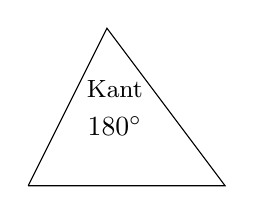
\begin{tikzpicture}
\draw (0,0) -- (1,2) -- (2.5,0) -- (0,0);
\draw (1.1,1) node[anchor=south]{\small Kant}node[anchor=north]{$180^\circ$};
\end{tikzpicture}
\column{.7\textwidth}
\begin{itemize}
	\item Geometry --- pure intuition of space
	\item Arithmetic --- pure intuition of time $1+1=2$
\end{itemize}
\begin{description}
	\item[Kant] Mathematics is synthetic a priori.
	\item[Frege] Mathematics is analytic.
\end{description}
\end{columns}
\end{frame}

\begin{frame}\frametitle{Causation --- Aristotle's Four Causes}
\begin{figure}[H]
\includegraphics[width=.9\textwidth]{img/4causes.png}
\end{figure}
\end{frame}

\begin{frame}\frametitle{Causation}
\vspace*{-1ex}
\begin{itemize}
	\item Mill's Sufficient Condition: $A$ causes $B$ iff $A\to B$.
	\item Hobbes's Necessary Condition: $A$ causes $B$ iff $\neg A\to\neg B$.
	\item Probabilistic Causation: $A$ causes $B$ iff 
	\begin{itemize}
		\item Reichenbach: $P(B\mid A)>P(B\mid \neg A)$
		\item Cartwright: $P(B\mid A\wedge C)>P(B\mid \neg A\wedge C)$ for background context $C$.
		\item Dupr\'e: $\sum_C P(C)\big[P(B\mid A\wedge C)-P(B\mid \neg A\wedge C)\big]>0$
	\end{itemize}
	\item Fair's Transference Theory: $A$ causes $B$ iff there is a transfer of energy or momentum from $A$ to $B$.
	\item Woodward's Manipulability Theory: $A$ causes $B$ iff one can manipulate the world such as to make $A$ occur in order to produce $B$.
	\item Hume:	``We may define a cause to be an object followed by another, and where all the objects, similar to the first, are followed by objects similar to the second. Or, in other words, where, if the first object had not been, the second never had existed.''
	\item Lewis: ``$A$ causes $B$'' iff ``$B$ would not have occurred if not for $A$.''
	\item ``if it were the case that $A$ then it would be 		the case that $B$'' is true iff among all $A$-worlds (i.e., worlds in which $A$ is true) some $B$-worlds are closer to the actual world than all $\neg B$-worlds.
\end{itemize}
\end{frame}

\begin{frame}\frametitle{David Lewis 1941–2001}
\centerline{\textcolor{red}{Counterfactual Causation}}
\[\textcolor{red}{A\boxright B}\]
\begin{figure}[H]
\includegraphics[width=.45\textwidth]{img/lewis.jpg}	
\end{figure}
\end{frame}

\begin{frame}\frametitle{Antecedent Strengthenng}
\begin{align*}
	A\to C&\vDash A\wedge B\to C\\
	A\boxright C&\nVdash A\wedge B\boxright C
\end{align*}
\begin{enumerate}
	\item If the match were struck, it would light.
	\item Therefore, if the match were struck in outer space, it would light.
\end{enumerate}
The closest world where I light the match and I do so in outer space is much further removed from the actual world than the closest world where I light the match is.
\end{frame}

\begin{frame}\frametitle{Transitivity}
\begin{align*}
	A\to B, B\to C&\vDash A\to C\\
	A\boxright B, B\boxright C&\nVdash A\boxright C
\end{align*}
\begin{enumerate}
	\item If J.~Edgar Hoover had been born a Russian, he would have been a Communist.
	\item If J.~Edgar Hoover were a Communist, he would have been be a traitor.
	\item Therefore, If J.~Edgar Hoover had been born a Russian, he would have been be a traitor.
\end{enumerate}
\end{frame}

\begin{frame}\frametitle{Contraposition}
\begin{align*}
A\to B&\vDash \neg B\to \neg A\\
A\boxright B&\nVdash \neg B\boxright \neg A
\end{align*}
\begin{enumerate}
	\item If Goethe hadn't died in 1832, he would (still) be dead now.
	\item If Goethe weren't dead now, he would have died in 1832.
\end{enumerate}
\end{frame}

\begin{frame}\frametitle{Minimal Change Semantics}
\begin{definition}[Sphere Model]
A \emph{sphere model} is a triple $\mathcal{M} = \{W,O,V\}$, where $W\ne\emptyset$, $V:\operatorname{Atom} \to \operatorname{P}(W)$, and $O: W \to \operatorname{P}(\operatorname{P}(W))$ assigns to each
 world $w$ a \emph{system of spheres} $O_w$. For each $w$, $O_w$ is a set of sets of worlds such that:
 \begin{enumerate}
 \item $O_w$ is \emph{centered} on $w$: $\{w\} \in O_w$.
 \item $O_w$ is \emph{nested}: whenever $S_1$, $S_2 \in O_w$, $S_1 \subset S_2$ or $S_2 \subset S_1$.
 \item $O_w$ is closed under non-empty unions.
 \item $O_w$ is closed under non-empty intersections.
 \end{enumerate}	
\end{definition}
\begin{definition}[Counterfactual Conditional]
$\mathcal{M},w\Vdash A\boxright B$ iff either
\begin{enumerate}
	\item for all $v\in\bigcup O_w: \mathcal{M},v\nVdash A$, or
	\item for some $S\in O_w$,
	\begin{enumerate}
		\item $\mathcal{M},v\Vdash A$ for some $v\in S$, and
		\item for all $v\in S: \mathcal{M},v\Vdash A\to B$.
	\end{enumerate}
\end{enumerate}
\end{definition}
\end{frame}

\begin{frame}\frametitle{Minimal Change Semantics}
	\begin{figure}[H]
		\includegraphics[width=.5\textwidth]{img/counterfactual.pdf}
	\end{figure}
\begin{problem}
How do humans represent ``possible worlds'' in their minds and compute the closest one, when the number of possibilities is far beyond the capacity of the human brain?
\end{problem}
\end{frame}

\begin{frame}\frametitle{}
\[
\infer{\bigwedge\limits_{i=1}^n (A\boxright B_i)\to(A\boxright C)}{\bigwedge\limits_{i=1}^n B_i\to C}
\]
\begin{itemize}
	\item $A\boxright A$
	\item $(A\boxright B)\wedge (B\boxright A)\to(A\boxright C)\leftrightarrow(B\boxright C)$
	\item $((A\vee B)\boxright A)\vee((A\vee B)\boxright B)\vee(((A\vee B)\boxright C)\leftrightarrow(A\boxright C)\wedge(B\boxright C))$
	\item $(\neg A\boxright A)\to(B\boxright A)$
	\item $(A\boxright \neg B)\vee((A\wedge B\boxright C)\leftrightarrow(A\boxright(B\to C)))$
	\item $(A\boxright B)\to(A\to B)$
	\item $A\wedge B\to (A\boxright B)$
\end{itemize}
\end{frame}

\begin{frame}\frametitle{Gettier Problem: Is Justified True Belief Knowledge?}
\begin{figure}
\includegraphics[width=.6\textwidth]{img/knowledge-true-belief.png}
\end{figure}
\begin{enumerate}
	\item Smith believes \textbf{``Bob owns a Ford''}.
	\item He was told this by Bob.
	\item Bob then sells his Ford.
	\item Meanwhile Bob wins a Ford in a raffle.
\end{enumerate}
\end{frame}

\begin{frame}\frametitle{Epistemic Justification}
\begin{figure}
\subfigure{\includegraphics[height=.2\textwidth]{img/foundationalism.jpeg}}
\subfigure{\includegraphics[height=.2\textwidth]{img/coherentism.png}}
\end{figure}
\begin{itemize}
\item Internalist theory of epistemic justification.
\begin{itemize}
	\item Foundationalism\\
	--- $S$'s belief $p$ is justified iff either
	\begin{enumerate}[(a)]
		\item $p$ is a basic belief; or
		\item $p$ is a non-basic belief justified inferentially by $S$'s basic beliefs.
	\end{enumerate}
	\item Coherentism\\
	--- $S$'s belief $p$ is justified iff $S$ has a coherent set of beliefs which includes $p$.
\end{itemize}
\item Externalist theory of epistemic justification.
\begin{itemize}
	\item Reliabilism\\
	--- $S$'s belief $p$ is justified iff $p$ is produced by a reliable cognitive process.
\end{itemize}
\end{itemize}
\end{frame}

\begin{frame}\frametitle{Nozick's Truth-Tracking Condition}
\begin{block}{Nozick's Truth-Tracking Condition}
$S$ knows that $p$ iff:
\begin{enumerate}
	\item $p$ is true;
	\item $S$ believes that $p$;
	\item if $p$ were not true, $S$ would not believe that $p$;
	\item if $p$ were true, $S$ would believe that $p$.
\end{enumerate}
\end{block}
\begin{block}{Kripke's Counterexample --- Fake Barn Country}
\begin{itemize}
	\item Smith is driving in a country containing fake barns.
	\item The fake barns are painted green.
	\item In the midst of these fake barns is one real barn, which is painted red.
	\begin{enumerate}
	\item Smith looks up and happens to see the real barn. \textbf{``I see a red barn.''}
	\item What if Smith looks up and forms the belief \textbf{``I see a barn''}?
	\begin{itemize}
	\item Though Smith has gotten lucky, he could have just as easily been deceived and not have known it.
	\end{itemize}
	\end{enumerate}
\end{itemize}		
\end{block}
\end{frame}

\begin{frame}\frametitle{Skepticism}
\begin{enumerate}[$S_1$]
	\item I know ``I have hands''.\hfill $Kp$
	\item If I know ``I have hands'' then I know ``I am not a brain in the vat''.\par\hfill $K(p\to q)$
	\item I don't know that ``I am not a brain in the vat''.\hfill $\neg Kq$
\end{enumerate}
\begin{itemize}
	\item I fail to know that ``I am not a brain in the vat'' since I would falsely believe ``I was not a brain in the vat'' in the closest world in which I am a brain in the vat.
	\item Nozick's definition of Knowledge $Kp\coloneqq p\wedge Bp\wedge (\textcolor{red}{\neg p\boxright\neg Bp})\wedge (p\boxright Bp)$ is not closed under known entailment.
	\[Kp,K(p\to q)\nVdash Kq\]
	\item If we use Sosa's definition, $Kp\coloneqq p\wedge Bp\wedge (\textcolor{red}{Bp\boxright p})\wedge (p\boxright Bp)$, then 
	\[Kp,K(p\to q)\Vdash Kq\]
\end{itemize}
\end{frame}

%--------------------------%
\subsection{Probability}
%--------------------------%

\begin{frame}\frametitle{Uncertainty, Ignorance, Vagueness}
Some Approaches:
\begin{itemize}
	\item Logic-based systems with weights attached to rules
	\item Dempster-Shafer Theory: represents `ignorance' \& `uncertainty'
	\begin{itemize}
		\item basic belief assignment function $m:2^X\to[0,1]$
		\item belief: $\operatorname{bel}(A)\coloneqq\sum\limits_{{B: B\subset A}}m(B)$
		\item plausibility: $\operatorname{pl}(A)\coloneqq\sum\limits_{{B: B\cap A\ne\emptyset}}m(B)$
		\item Dempster's rule of combination
		\[(m_1\oplus m_2)(A)\coloneqq\frac{\sum\limits_{B\cap C=A}m_1(B)m_2(C)}{1-\sum\limits_{{B\cap C=\emptyset}}m_1(B)m_2(C)}\]
	\end{itemize}
	\item Fuzzy logic and fuzzy sets: represents `vagueness', not `uncertainty'.
	\item Bayesian Network
\end{itemize}
\end{frame}

\begin{frame}\frametitle{Uncertainty and Probability}
\begin{itemize}
	\item Frequentist: probabilities are relative frequencies.\\
	(e.g. the relative frequency of tossing head.)
	\[P(E)=\lim\limits_{n\to\infty}\frac{n_E}{n}\]
	\begin{itemize}
		\item Frequency Interpretation is Circular --- For fair coin, $P(H) = 1/2$ with ``high probability''. But to make this statement rigorous we need to formally know what ``high probability'' means. \hfill \textcolor{red}{Circularity!}
		\item Reference Class Problem
		\item Limited to I.I.D
	\end{itemize}
	\item Objectivist: probabilities are real aspects of the world.\\
	(e.g. the probability that some atom decays in the next hour)
	\item Subjectivist: probabilities describe an agent's degree of belief.\\
	(e.g. it is (im)plausible that extraterrestrians exist)
	\begin{itemize}
		\item Cox's Theorem
		\item Dutch Book
	\end{itemize}
\end{itemize}
\end{frame}

\begin{frame}\frametitle{Objective Probability $=$ Inter-Subjective Probability?}
\begin{itemize}
	\item The assumption that an event occurs with some objective probability expresses the opinion that the occurrence of an individual stochastic event has no explanation.\\
	$\implies$ i.e. the event is inherently impossible to predict for sure.
	\item One central goal of science is to explain things.
	\item If a sufficiently large community of people arrive at the same subjective probabilities from their prior knowledge, one may want to call these probabilities objective.
	\item Example $1$: The outcome of tossing a coin is usually agreed upon to be random, but may after all be predicted by taking a close enough look.
	\item Eaxmple $2$: Even quantum events may be only pseudo-random.
\end{itemize}	
\end{frame}

\begin{frame}\frametitle{Probability}
\begin{columns}
\column{.5\textwidth}
\begin{gather*}
\text{(objective) chance}\\
\downarrow\\
\text{how to measure?}\\
\downarrow\\
\text{frequency of occurrence}
\end{gather*}
\column{.5\textwidth}
\begin{gather*}
\text{(subjective) degree of belief}\\
\downarrow\\
\text{how to measure?}\\
\downarrow\\
\text{gambling behaviour}
\end{gather*}
\end{columns}
\vspace*{4ex}
\centerline{Kolmogorov's Axioms of probability must apply to both!}
\end{frame}

\begin{frame}\frametitle{Probability Space}
A \emph{$\sigma$-algebra} $\mathcal{A}$ is a collection of subsets of the sample space $\Omega$ s.t.
\begin{enumerate}
	\item $\Omega\in\mathscr{A}$
	\item $A,B\in\mathscr{A}\implies A\cap B, A\cup B\in\mathscr{A}$
	\item $A\in\mathscr{A}\implies \Omega\setminus A\in\mathscr{A}$
	\item $\forall i\geq 1\left(A_i\in\mathscr{A}\implies\bigcup\limits_{i\geq 1}A_i\in\mathscr{A}\right)$
\end{enumerate}
$(\Omega,\mathscr{A})$ is a \emph{measurable space} iff $\mathscr{A}\subset \operatorname{P}(\Omega)$ is a $\sigma$-algebra.

$(\Omega,\mathscr{A},P)$ is a \emph{probability space} iff $P$ is a probability measure on $\mathscr{A}$ s.t.
\begin{enumerate}
	\item $P(A)\geq 0$ for $A\in\mathscr{A}$
	\item $\operatorname{P}(\Omega)=1$
	\item $A_i\in\mathscr{A}\;\;\&\;\; A=\biguplus\limits_{i=1}^\infty A_i \implies P(A)=\sum\limits_{i=1}^\infty P(A_i)$
\end{enumerate}

A \emph{filtration} on $(\Omega,\mathscr{A})$ is a sequence $(\mathscr{A}_t)_{t\geq 0}$ of $\sigma$-algebras s.t. 
\[\forall t\left(\mathscr{A}_{t} \subseteq \mathscr{A}\right)\;\;\text{and}\;\;\forall t_1,t_2\left(t_1\leq t_2 \implies \mathscr{A}_{t_1} \subseteq \mathscr{A}_{t_2}\right)\]

$(\Omega,\mathscr{A},(\mathscr{A}_t)_{t\geq 0},P)$ is a \emph{filtered probability space}.
\end{frame}

\begin{frame}\frametitle{Probability}
Probabilistic assertions summarize effects of
\begin{itemize}
	\item laziness: failure to enumerate exceptions, qualifications, etc.
	\item ignorance: lack of relevant facts, initial conditions, etc.
\end{itemize}
Subjective probabilities relate propositions to one's own state of knowledge. They summarize the agent's beliefs.\\
\begin{itemize}
	\item A random variable is a function from sample points to some range, e.g. the reals or Booleans.
	\item Think of a proposition as the event (set of sample points) where the proposition is true.
\[P(X=x)=\sum\limits_{u:X(u)=x}P(u)\qquad P(A)=\sum\limits_{u\vDash A}P(u)\]
\[P(\operatorname{DiceOdd}=\operatorname{true})=P(1)+P(3)+P(5)=\frac{1}{6}+\frac{1}{6}+\frac{1}{6}=\frac{1}{2}\]
\end{itemize}
\end{frame}

\begin{frame}\frametitle{}
	\resizebox{1.02\textwidth}{!}{$
		\begin{array}{c|c}
		\hline
		A\implies B & P(B\mid A)=1\\
		\hline
		A\implies \neg B & P(B\mid A)=0\\
		\hline
		\vdash A\to(B\to A) & P(A\mid AB)=1\\
		\hline
		\vdash (A\to B)\to (B\to C)\to (A\to C) & P(C\mid A)\geq P(C\mid B)P(B\mid A)\\
		\hline
		\vdash(\neg B\to\neg A)\to(A\to B) & P(B)\geq 1-\dfrac{1-P(A)}{P(\neg A\mid\neg B)}\\
		\hline
		\vdash A\vee\neg A & P(A)+P(\neg A)=1\\
		\hline
		\vdash\neg(A\wedge\neg A) & P(A\wedge\neg A)=0\\
		\hline
		\vdash\neg(A\vee B)\leftrightarrow\neg A\wedge\neg B & P(\neg(A\vee B))=P(\neg A)P(\neg B)\\
		\hline
		\vdash(A\to B)\wedge A\to B & P(B)\geq P(B\mid A)P(A)\\
		\hline
		\nvdash (A\to B)\to (B\to A) & P(B\mid A)=1\centernot\Longrightarrow P(A\mid B)=1\\
		\hline
		\nvdash (A\to B)\to (B\to A) & P(B\mid A)>P(B)\implies P(A\mid B)>P(A)\\
		\hline
		\varphi(0)\wedge\forall n(\varphi(n)\to\varphi(n+1))\to\forall n\varphi(n) &
		\begin{matrix}
		P(A_n)\geq \prod\limits_{i=1}^{n-1} P(A_{i+1}\mid A_i)\\
		\forall i<n (P(A_{i+1}\mid A_i)=1)\implies P(A_n)=1\\
		\forall i,j (P(A_{i+1}\mid A_i)=P(A_{j+1}\mid A_j)<1)\implies \prod\limits_{i=1}^\infty P(A_{i+1}\mid A_i)=0
		\end{matrix}\\
		\hline
		\varphi(0)\wedge\forall n(\varphi(n)\to\varphi(n+1))\to\forall n\varphi(n) &
		\begin{matrix}
		P(X=X_1)\geq c \;\&\;\cdots\;\&\; P(X=X_n)\geq c\\
		\Downarrow\\
		P(X=X_1=\cdots =X_n\mid X_1=\cdots =X_n)\geq\dfrac{c^n}{c^n+(1-c)^n}
		\end{matrix}\\
		\hline
		\varphi(0)\wedge\forall n(\varphi(n)\to\varphi(n+1))\to\forall n\varphi(n) &
		\begin{matrix}
		\forall i (P(A_{i+1}\mid A_i)>0)\\
		\Downarrow\\
		\hspace{1.1cm}\prod\limits_{i\geq 1} P(A_{i+1}\mid A_i)=0\iff\sum\limits_{i\geq 1} \left(1-P(A_{i+1}\mid A_i)\right)=\infty
		\end{matrix}\\
		\hline
		\end{array}$
	}
\end{frame}

\begin{frame}\frametitle{Logic, Belief, Probability --- Cox Theorem}
\begin{center}
\fbox{Probability theory extends propositional logic?}
\end{center}
\begin{assumption}[Cox's Assumptions for Beliefs]
\begin{enumerate}
	\item $A\leftrightarrow B\implies b(\cdot\mid A)=b(\cdot\mid B)\;\&\;b(A\mid\cdot)=b(B\mid\cdot)$.
	\item there is a continuous binary operation $\otimes$ that is strictly increasing in each coordinate s.t. $b(A\wedge B\mid C)=b(A\mid C)\otimes b(B\mid A\wedge C)$.
	\item for any rational numbers $r_1,r_2,r_3\in (0,1)$ there are $A,B,C,D\in\Omega$ s.t. $r_1=b(A\mid D)$, $r_2=b(B\mid A\wedge D)$ and $r_3=b(C\mid A\wedge B\wedge D)$.
	\item thers is a continuous nonnegative nonincreasing function $N: [0,1]\to [0,1]$ s.t. $b(\neg A\mid C)=N(b(A\mid C))$.
\end{enumerate}
\end{assumption}
\begin{theorem}[Cox Theorem]
A credence function that satisfies Cox's assumptions for beliefs is isomorphic to a probability function.
\end{theorem}
\end{frame}

\begin{frame}\frametitle{Why are the Axioms of Probability Theory Reasonable?}
\begin{itemize}
	\item If $P$ represents an objectively observable probability, the axioms clearly make sense.
	\item But why should an agent respect these axioms when it models its own degree of belief?
\end{itemize}
\begin{block}{Dutch Book Argument --- Ramsey/de Finetti}
If the beliefs do not follow the Kolmogorov axioms, then there exists a betting strategy against the agent, where he will definitely loose!
\end{block}
Peirce/Putnam: a belief is true if it would be accepted by anyone under ideal epistemic conditions.
\end{frame}

\begin{frame}\frametitle{Inference}
\begin{itemize}
	\item Probability is a rigorous formalism for uncertain knowledge.
	\item Joint probability distribution specifies probability of every atomic event.
	\item Queries can be answered by summing over atomic events.
\end{itemize}
\begin{itemize}
	\item Bayes Rule
	\[P(Y\mid X)=\frac{P(X\mid Y)P(Y)}{P(X)}\]
	\item Marginalization $P(X)=\sum\limits_y P(X,y)=\sum\limits_y P(X\mid y)P(y)$
	\item General idea: compute distribution on query variable by fixing evidence variables and summing over hidden variables.
	\item Let $S$ be the hidden variables. We want the posterior joint distribution of the query variables $H$ given specific values $e$ for the evidence variables $E$.
\end{itemize}
\[P(H\mid E=e)=\frac{P(H,E=e)}{P(E=e)}=\frac{\sum\limits_{s}P(H,E=e,S=s)}{P(E=e)}\]
\end{frame}

\begin{frame}\frametitle{Digression --- Jeffery's Radical Probabilism Philosophy}
\centerline{\fbox{\textcolor{red}{What is a rational update $P_{\mathrm{old}}\to P_{\mathrm{new}}$?}}}
\begin{itemize}
\item Dogmatic Probabilism: any rational change in beliefs should be explained by a Bayesian update.
\begin{block}{Bayesian Update}
\[P_{\mathrm{new}}(B)=P_{\mathrm{old}}(B\mid A)\]
\end{block}
\item Radical Probabilism: no facts are known for certain.
\begin{block}{Jeffrey Update}
\[P_{\mathrm{new}}(B)=P_{\mathrm{new}}(A)\cdot P_{\mathrm{old}}(B\mid A)+P_{\mathrm{new}}(\neg A)\cdot P_{\mathrm{old}}(B\mid \neg A)\]
\end{block}
\item van Fraassen's Reflection Principle
\[P_0(A\mid P_1(A)=x)=x\]
\end{itemize}
\end{frame}

\begin{frame}\frametitle{}
\begin{itemize}
	\item expected value (or mean) $\mathbb{E}[X]\coloneqq\sum\limits_x xP(X=x)$
	\item conditional mean $\mathbb{E}[Y\mid X=x]\coloneqq\sum\limits_y yP(Y=y\mid X=x)$
	\item variance $\operatorname{Var}(X)\coloneqq \mathbb{E}\left[(X-\mathbb{E}[X])^2\right]=\mathbb{E}[X^2]-\mathbb{E}[X]^2$
	\item covariance of $X$ and $Y$
	\[\operatorname{Cov}(X,Y)\coloneqq\mathbb{E}\big[(X-\mathbb{E}[X])(Y-\mathbb{E}[Y])\big]\]
	\item correlation coefficient
	\[\rho_{XY}\coloneqq\frac{\operatorname{Cov}(X,Y)}{\sqrt{\operatorname{Var}(X)\operatorname{Var}(Y)}}\]
	\item regression coefficient of $X$ on $Y$
	\[r_{XY}\coloneqq\rho_{XY}\frac{\sqrt{\operatorname{Var}(X)}}{\sqrt{\operatorname{Var}(Y)}}=\frac{\operatorname{Cov}(X,Y)}{\operatorname{Var}(Y)}\]
\end{itemize}
\[X\perp Y\implies \rho_{XY}=0\]
\[\rho_{XY}=0\centernot\implies X\perp Y\]
\centerline{No correlation does not imply independence}
\end{frame}

\begin{frame}\frametitle{No correlation does not imply independence}
\begin{itemize}
	\item $P(X=x)=\frac{1}{3}$ for $x=-1,0,1$
	\item $Y=X^2$
	\item $\operatorname{Cov}(X,Y)=0$
	\item $\rho_{X,Y}=0$
\end{itemize}
\end{frame}

\begin{frame}\frametitle{Conditional Independence}
\begin{definition}[Conditional Independence]
Let $V=\{V_1,V_2,\dots\}$ be a finite set of variables. Let $P(\cdot)$ be a joint probability function over the variables in $V$, and let $X,Y,Z$ stand for any three subsets of variables in $V$. The sets $X$ and $Y$ are said to be conditionally independent given $Z$ if
\[P(x\mid y,z)=P(x\mid z)\qquad \mbox{whenever } P(y,z)>0\]	
\end{definition}
\[(X\perp Y\mid Z)_P\quad\mbox{iff}\quad P(x\mid y,z)=P(x\mid z)\;\mbox{ for all } x,y,z \mbox{ s.t. } P(y,z)>0\]
\begin{description}
	\item[Symmetry] $(X\perp Y\mid Z)\implies (Y\perp X\mid Z)$
	\item[Decomposition] $(X\perp YW\mid Z)\implies (X\perp Y\mid Z)$
	\item[Weak union] $(X\perp YW\mid Z)\implies (X\perp Y\mid ZW)$
	\item[Contraction] $(X\perp Y\mid Z)\;\&\;(X\perp W\mid ZY)\implies (X\perp YW\mid Z)$
	\item[Intersection] $(X\perp W\mid ZY)\;\&\;(X\perp Y\mid ZW)\implies (X\perp YW\mid Z)$
\end{description}
\end{frame}

\begin{frame}\frametitle{Law of Large Number}
\begin{theorem}[(Weak/Strong) Law of Large Number]
Let $X_1,X_2,\dots,X_n$ be independent identically distributed random variables with $\mathbb{E}[X_i]=\mu$ and finite variance. Let $\overline{X}_n\coloneqq \frac{1}{n}\sum\limits_{i=1}^n X_i$. Then
\[\forall\varepsilon: \lim\limits_{n\to\infty}P\left(\left|\overline{X}_n-\mu\right|<\varepsilon\right)=1\tag{weak}\]
\[\lim\limits_{n\to\infty}P\left(\overline{X}_n=\mu\right)=1\tag{strong}\]
\end{theorem}
\end{frame}

\begin{frame}\frametitle{The Central Limit Theorem}
\begin{figure}[H]
\includegraphics[width=.67\textwidth]{img/clt.png}
\end{figure}
\begin{theorem}[Lindeberg-L\'evy Central Limit Theorem]
Let $X_1,X_2,\dots,X_n$ be independent identically distributed random variables with $\mathbb{E}[X_i]=\mu$ and $\operatorname{Var}(X_i)=\sigma^2<\infty$. Let $\overline{X}_n\coloneqq \frac{1}{n}\sum\limits_{i=1}^n X_i$ and $Z_n\coloneqq \frac{\overline{X}_n-\mathbb{E}\big[\overline{X}_n\big]}{\sqrt{\operatorname{Var}\big(\overline{X}_n\big)}}=\frac{\overline{X}_n-\mu}{\sigma/\sqrt{n}}$. Then
\[\lim\limits_{n\to\infty}P\left(Z_n<a\right)=\Phi(a)=\int_{-\infty}^a \frac{1}{\sqrt{2\pi}}\mathrm{e}^{-t^2/2}\mathrm{d}t\]
\end{theorem}
\end{frame}

%--------------------------%
\subsection{Bayesian Network}
%--------------------------%

\begin{frame}\frametitle{Judea Pearl 1936--}
\begin{figure}[H]
\includegraphics[width=\textwidth]{img/pearl0.jpg}	
\end{figure}
\end{frame}

\begin{frame}\frametitle{Bayesian Network}
\begin{definition}[Bayesian Network]
A Bayesian network is described as a directed acyclic graph $G = (V,E,P)$, whose nodes $V$ represent random variables, and edges $E\subset V\times V$ express dependences between nodes, and the joint probability distribution $P$ over $V$ is factorized as
\[P(V)=\prod\limits_{V_i\in V}P(V_i\mid\operatorname{PA}_i)\]
where $\operatorname{PA}_i$ is the set of parent nodes of $V_i$.
\end{definition}
\end{frame}

\begin{frame}\frametitle{Independent Causal Mechanisms}
\begin{block}{Independent Causal Mechanisms}
The causal generative process of a system's variables is composed of autonomous modules that do not inform or influence each other.\\
In the probabilistic case, this means that the conditional distribution of each variable given its causes (i.e. its mechanism) does not inform or influence the other conditional distributions.
\end{block}
\textbf{Remark:} changing one $P(V_i\mid\operatorname{PA}_i)$ does not change the other $P(V_j\mid\operatorname{PA}_j)$, $j\ne i$.\\
Knowing some other mechanism $P(V_j\mid\operatorname{PA}_j)$, $j\ne i$ does not give us information about a mechanism $P(V_i\mid\operatorname{PA}_i)$.
\end{frame}

\begin{frame}\frametitle{Markov Blanket}
\begin{itemize}
	\item A node is conditionally independent of all others given its \textbf{Markov blanket}: parents $+$ children $+$ children's parents.
\end{itemize}
\begin{figure}[H]
\includegraphics[width=.6\textwidth]{img/markov-blanket.pdf}
\end{figure}
\end{frame}

\begin{frame}\frametitle{Example: Bayesian network for the fire alarm problem}
\begin{figure}[H]
	\includegraphics[width=.8\textwidth]{img/bayesian-network.pdf}
\end{figure}
\end{frame}

\begin{frame}\frametitle{Markov Chain}
\begin{itemize}
	\item A Markov chain is a special sort of belief network.
\[
\begin{tikzcd}
S_0 \arrow[r] \& S_1 \arrow[r] \& S_2 \arrow[r] \& S_3 \arrow[r] \& S_4
\end{tikzcd}
\]
	\item $P(S_{t+1}\mid S_0,\dots,S_t)=P(S_{t+1}\mid S_t)$
	\item $S_t$ conveys all of the information about the history that can affect the future states.
	\item ``The past is independent of the future given the present.''
\end{itemize}
\end{frame}

\begin{frame}\frametitle{Hidden Markov Model}
\begin{itemize}
	\item A Hidden Markov Model (HMM) is a Bayesian network.
\[
\begin{tikzcd}
S_0 \arrow[r] \arrow[d] \& S_1 \arrow[r] \arrow[d] \& S_2 \arrow[r] \arrow[d] \& S_3 \arrow[r] \arrow[d] \& S_4 \arrow[d] \\
O_0 \& O_1 \& O_2 \& O_3 \& O_4
\end{tikzcd}
\]
	\item $P(S_0)$ specifies initial conditions
	\item $P(S_{t+1}\mid S_t)$ specifies the dynamics
	\item $P(O_t\mid S_t)$ specifies the sensor model
\end{itemize}
\end{frame}

\begin{frame}\frametitle{Constructing Bayesian Network}
To represent a domain in a Bayesian network, you need to
consider:
\begin{itemize}
	\item What are the relevant variables?
	\begin{itemize}
		\item What will you observe?
		\item What would you like to find out (query)?
		\item What other features make the model simpler?
	\end{itemize}
	\item What values should these variables take?
	\item What is the relationship between them? This should be expressed in terms of local influence.
	\item How does the value of each variable depend on its parents? This is expressed in terms of the conditional probabilities.
\end{itemize}
\end{frame}

\begin{frame}\frametitle{Bayesian Network Structure Learning}
\begin{itemize}
	\item Search over total orderings of variables.
	\item For each total ordering $X_1,\dots,X_n$ use supervised learning to learn $P(X_i\mid X_1,\dots,X_{i-1})$.
	\item Return the network model found with minimum:
	\[-\log P(\operatorname{examples}\mid\operatorname{network}) - \log P(\operatorname{network})\]
	where $\log P(\operatorname{network})$ decomposes into the sum of the representations for each variable.
\end{itemize}
\end{frame}

%--------------------------%
\subsection{Decision Network}
%--------------------------%

\begin{frame}\frametitle{Decision Network}
\begin{itemize}
	\item A decision network is a graphical representation of a finite sequential decision problem.
	\item Decision networks extend Bayesian networks to include \textcolor{yellow}{decision variables} and \textcolor{yellow}{utility}.
	\item A decision network specifies what information is available when the agent has to act.
	\item A decision network specifies which variables the utility depends on.
\end{itemize}
\end{frame}

\begin{frame}\frametitle{Example: decision network for the fire alarm problem}
\begin{figure}[H]
\includegraphics[width=.9\textwidth]{img/decision-network.pdf}
\end{figure}
\end{frame}

\begin{frame}\frametitle{Markov Decision Process}
\begin{figure}[H]
	\includegraphics[width=\textwidth]{img/decision-network-mdp.pdf}
	\caption{Decision network representing a finite part of an MDP}
\end{figure}
\end{frame}

\begin{frame}\frametitle{Partially Observable Markov Decision Process}
\begin{figure}[H]
	\includegraphics[width=\textwidth]{img/decision-network-pomdp.pdf}
	\caption{A POMDP as a dynamic decision network}
\end{figure}
\end{frame}

%--------------------------%
\subsection{What is Causal Inference?}
%--------------------------%

\begin{frame}\frametitle{}
\begin{figure}[H]
\includegraphics[width=\textwidth]{img/cave.jpg}	
\end{figure}
Do not model the distribution of the data, but model the mechanisms that generated the data!
\end{frame}

\begin{frame}\frametitle{Causal Inference vs Probabilistic Inference}
\[
\begin{tikzcd}
|[style={rectangle,draw}]| \textit{causal model} \arrow[ddddd,"subsumes" swap,dashed] \arrow[rrrrr,bend right=13,"\text{causal reasoning}" swap] \&\&\&\&\& |[style={rectangle,draw}]| \textit{$\stackrel{\textit{observation/outcomes incl.}}{\small\textit{changes/interventions}}$} \arrow[lllll,bend right=13,"\text{causal learning}" swap] \arrow[ddddd,"subsume",dashed] \\
\&\\
\&\\
\&\\
\&\\
|[style={rectangle,draw}]| \textit{probabilistic model} \arrow[rrrrr,bend right=13,"\text{probabilistic reasoning}" swap] \&\&\&\&\& |[style={rectangle,draw}]| \textit{observations/outcomes} \arrow[lllll,bend right=13,"\text{statistical learning}" swap]
\end{tikzcd}
\]
\end{frame}

\begin{frame}\frametitle{}
\begin{figure}[H]
\includegraphics[width=\textwidth]{img/causal-inference.pdf}	
\end{figure}
\end{frame}

\begin{frame}\frametitle{Causal Model}
\begin{itemize}
	\item A causal model lets you predict the effect of an intervention.
	\item Not all Bayesian networks are causal.
	\item A causal network is a Bayesian network with the requirement that the relationships be causal.
	\item We can't learn causal models from observational data unless you are prepared to make modeling assumptions.
	\item We can learn causal models from randomized control trial.
\end{itemize}
\textbf{Example:} Inferring the effects of any treatment/policy/intervention/etc.
\begin{itemize}
	\item Effect of treatment on a disease
	\item Effect of climate change policy on emissions
	\item Effect of social media on mental health
\end{itemize}
\end{frame}

\begin{frame}\frametitle{Causal Inference Engine}
\begin{figure}[H]
\includegraphics[width=\textwidth]{img/causal-inference-engine.pdf}		
\end{figure}	
\end{frame}

\begin{frame}\frametitle{The Ladder of Causation}
\begin{figure}[H]
\includegraphics[height=.7\textwidth]{img/ladder.jpg}	
\end{figure}
\end{frame}

\begin{frame}\frametitle{The Ladder of Causation}
\vspace{-1ex}
\begin{scriptsize}
\begin{block}{$3$ Counterfactuals $P(Y_{X=x'}\mid X=x,Y_{X=x}=y)$}
\begin{itemize}
	\item \textbf{Activity:} Imagining, Retrospection, Understanding
	\item \textbf{Questions:} What if I \textcolor{red}{had done} \dots? Why?\\
	(Was it $X$ that caused $Y$? What if $X$ had not occured? What if I had acted differently?)
	\item \textbf{Examples:} Was it the aspirin that stopped my headache?\\
	Would Kennedy be alive if Oswald had not killed him?\\
	What if I had not smoked for the last $2$ years?
\end{itemize}
\end{block}
\vspace{-1ex}
\begin{block}{$2$ Intervention $P(Y\mid \operatorname{do}(X=x))$}
\begin{itemize}
	\item \textbf{Activity:} Doing, Intervening
	\item \textbf{Questions:} What if I do \dots? How?\\
	(What would $Y$ be if I \textcolor{red}{do} $X$? How can I make $Y$ happen?)
	\item \textbf{Examples:} If I take aspirin, will my headache be cured?\\
	What if we ban cigarettes?
\end{itemize}
\end{block}
\vspace{-1ex}
\begin{block}{$1$ Association $P(Y\mid X=x)$}
\begin{itemize}
	\item \textbf{Activity:} Seeing, Observing
	\item \textbf{Questions:} What if I \textcolor{red}{see} \dots?\\
	(How are the variables related? How would seeing $X$ change my belief in $Y$?)
	\item \textbf{Examples:} What does a symptom tell me about a disease?\\
	What does a survey tell us about the election results?
\end{itemize}
\end{block}
\end{scriptsize}
\end{frame}

\begin{frame}\frametitle{}
\begin{figure}[H]
\includegraphics[width=\textwidth]{img/causal-inference-procedure.pdf}	
\end{figure}
\begin{block}{Graphical Representation}
\begin{description}
	\item[Association] Bayes Network
	\item[Intervention] Causal Bayes Network
	\item[Counterfactuals] Functional Causal Graph
\end{description}
\end{block}
\end{frame}

\begin{frame}\frametitle{The Causal Hierarchy}
\begin{enumerate}
	\item Association: ``What if I see $x$?'' \[P(y\mid x)\]
	\item Intervention: ``What if I do $x$?'' \[P(y\mid \operatorname{do}(x))\]
	\item Counterfactuals: ``What if I had done things differently?'' \[P(y_{x'}\mid x)\]
	\item Options: ``With what probability?''
\end{enumerate}
\begin{description}
	\item[Explanation] $y$ because of $x$
	\item[Intervention] $y$ will be true if I do $x$
	\item[Counterfactuals] $y$ would be different if $x'$ were true
\end{description}
\end{frame}

\begin{frame}\frametitle{Randomized Control Trial --- Deconfounding via ``Randomness''}
\[
\begin{tikzcd}[row sep=small, cells={nodes={draw=gray}}]
	\textit{Other} \arrow[dd] \arrow[ddrrr] \& \textit{Texture} \arrow[ddl] \arrow[ddrr] \& \textit{Drainage} \arrow[ddll] \arrow[ddr] \& \textit{Microflora} \arrow[ddlll] \arrow[dd] \\
	\&\\
	\textit{Fertilizer} \arrow[rrr] \&\&\& \textit{Yield}
\end{tikzcd}
\]
\[
\begin{tikzcd}[row sep=small, cells={nodes={draw=gray}}]
	\textit{Other} \arrow[ddrrr] \& \textit{Texture} \arrow[ddrr] \& \textit{Drainage} \arrow[ddr] \& \textit{Microflora} \arrow[dd] \\
	\&\\
	\textit{Fertilizer}=1 \arrow[rrr] \&\&\& \textit{Yield}
\end{tikzcd}
\]
\[
\begin{tikzcd}[row sep=small, cells={nodes={draw=gray}}]
	\textit{Other} \arrow[ddrrr] \& \textit{Texture} \arrow[ddrr] \& \textit{Drainage} \arrow[ddr] \& \textit{Microflora} \arrow[dd] \\
	\& |[openbox,red]| \textcolor{red}{\text{Random}} \arrow[dl,red,controls={+(-1.7,-0.5) and +(0,2)},dotted] \\
	\textit{Fertilizer}=1 \arrow[rrr] \&\&\& \textit{Yield}
\end{tikzcd}
\]
\end{frame}

\begin{frame}\frametitle{Randomized Control Trial}
\begin{figure}[H]
\includegraphics[width=.6\textwidth]{img/rct.png}		
\end{figure}	
\end{frame}

\begin{frame}\frametitle{Randomized Control Trial \& Covariate Balance}
\setlength\abovedisplayskip{0pt}
\setlength\belowdisplayskip{0pt}
\begin{itemize}
	\item Treatment and control groups are the same in all aspects except treatment.
	\item We have \emph{covariate balance} if the distribution of covariates $Z$ is the same across treatment groups. More formally,
\[P(Z\mid X=1) \stackrel{d}{=} P(Z\mid X=0)\qquad \mbox{($\stackrel{d}{=}$ means `equal in distribution')}\]
	\item Randomization implies covariate balance.
	\begin{gather*}
	\text{Randomization} \implies X\perp Z \\
	P(Z\mid X=1) \stackrel{d}{=} P(Z) \\
	P(Z\mid X=0) \stackrel{d}{=} P(Z) \\
	P(Z\mid X=1) \stackrel{d}{=} P(Z\mid X=0)
	\end{gather*}
	\item Covariate balance implies association is causation.
	\begin{align*}
		P(y\mid \operatorname{do}(x))&=\sum_zP(y\mid x,z)P(z)=\sum_z\frac{P(y\mid x,z)P(x\mid z)P(z)}{P(x\mid z)}\\
		&=\sum_z\frac{P(y,x,z)}{P(x)}=\sum_zP(y,z\mid x)=P(y\mid x)
	\end{align*}
\end{itemize}
\end{frame}

\begin{frame}\frametitle{Randomized Control Trial}
Can't always randomize treatment
\begin{itemize}
	\item Ethical reasons (e.g. unethical to randomize people to smoke for measuring effect on lung cancer)
	\item Infeasibility (e.g. can't randomize countries into communist/capitalist systems to measure effect on GDP)
	\item Impossibility (e.g. can't change a living person's DNA at birth for measuring effect on breast cancer)
\end{itemize}
\textbf{Question:} Can we compute causal effects from observational data and, thus, without performing interventions? Yes, but not always.
\end{frame}

\begin{frame}\frametitle{What if you cannot do a randomized control trial?}
\[
\begin{tikzcd}[cells={nodes={draw=gray}}]
\& \textit{Confounder} \arrow[dl] \arrow[dr] \\
\textit{Treatment} \arrow[r] \& \textit{Mediation} \arrow[r] \& \textit{Outcome}
\end{tikzcd}
\]
\[\text{How to infer causal relations from data without experiment?}\]
\[P(y\mid \operatorname{do}(x))\]
\end{frame}

%--------------------------%
\subsection{Structural Causal Model}
%--------------------------%

\begin{frame}\frametitle{Structural Causal Model}
\begin{definition}[Structural Causal Model]
	A structural causal model is a $4$-tuple $(U, V, F, P)$, where
	\begin{itemize}
		\item $U=\{U_1,\dots,U_m\}$ is a set of background variables that are determined by factors outside the model.
		\item $V=\{V_1,\dots,V_n\}$ is a set of endogenous variables that are determined by other variables in the model --- that is, variables in $U\cup V$.
		\item $F=\{f_1,\dots,f_n\}$ is a set of structural assignments, $V_i=f_i(\operatorname{PA}_i,U_i)$.
		\item $P$ is a distribution over $U$.
	\end{itemize}
	$P(U)$ and $F$ induce a distribution $P(V)$ over observable variables.
\end{definition}
\end{frame}

\begin{frame}\frametitle{Causal Graph}
\begin{definition}[Causal Graph]
Consider an structural causal model $M=(U,V,F,P)$. Then $G$ is said to be a causal graph of $M$ if constructed as follows:
\begin{enumerate}
	\item add a node for every endogenous variable in the set $V$.
	\item add an edge \begin{tikzcd}
		V_j \arrow[r] \& V_i
	\end{tikzcd} for every $V_i,V_j\in V$ if $V_j$ appears as an argument of $f_i\in F$.
	\item add a bidirected edge \begin{tikzcd}
			V_i \arrow[r,leftrightarrow,dashed] \& V_j
		\end{tikzcd} for every $V_i,V_j\in V$ if the corresponding $U_i,U_j\in U$ are correlated or the corresponding $f_i,f_j$ share the same background variable as an argument.
\end{enumerate}
\end{definition}
\textbf{Remark:} Each bidirected arrow encodes unobserved confounding in $G$. They indicate correlation between the unobserved parents of the endogenous variables at the endpoints of such edges.\\
\textbf{Remark:} $X$ is a \emph{direct cause} of $Y$ if $X$ is a parent of $Y$.\\
$X$ is a \emph{cause} of $Y$ if $X$ is an ancestor of $Y$.
\end{frame}

\begin{frame}\frametitle{Example}
\setlength\abovedisplayskip{0pt}
\setlength\belowdisplayskip{0pt}
\begin{columns}
\column{.5\textwidth}
\[
\begin{tikzcd}[row sep = small, cells={nodes={draw=gray}}]
\& \textit{Climate} \arrow[dl] \arrow[dr] \& \\
\textit{Sprinkler} \arrow[dr] \&\& \textit{Rain} \arrow[dl]\\
\& \textit{Wetness}
\end{tikzcd}
\]
\column{.4\textwidth}
\begin{align*}
&\textcolor{red}{{Model}(M)}\\
C&=f_C(U_C)\\
S&=f_S(C,U_S)\\
R&=f_R(C,U_R)\\
W&=f_W(S,R,U_W)
\end{align*}
\end{columns}
\begin{itemize}
	\item Every missing arrow advertises an independency, conditional on a separating set.
\[C\perp W\mid (S,R)\qquad S\perp R\mid C\]
	\item $P_{S=1}(C,R,W)=P(C)P(R\mid C)P(W\mid R,S=1)\ne P(C,R,W\mid S=1)$
\end{itemize}
\begin{columns}
\column{.5\textwidth}
\[
\begin{tikzcd}[row sep = small]
\& C \arrow[dr] \& \\
S=1 \arrow[dr] \&\& R \arrow[dl]\\
\& W
\end{tikzcd}
\]
\column{.4\textwidth}
\begin{align*}
&\textcolor{red}{\text{Model}(M_{S=1})}\\
C&=f_C(U_C)\\
S&=1\\
R&=f_R(C,U_R)\\
W&=f_W(S,R,U_W)
\end{align*}
\end{columns}
Would the pavement be wet \textbf{had} the sprinkler been on?
\end{frame}

\begin{frame}\frametitle{}
\begin{figure}[H]
\includegraphics[width=.5\textwidth]{img/chicken-egg.png}	
\end{figure}
\[f=ma\implies m=\frac{f}{a}\]
\begin{quote}
All philosophers imagine that causation is one of the fundamental axioms or postulates of science, yet, oddly enough, in advanced sciences such as gravitational astronomy, the word `cause' never occurs. The law of causality, I believe, like much that passes muster among philosophers, is a relict of a bygone age, surviving, like the monarchy, only because it is erroneously supposed to do no harm.\par
\hfill --- \textsf{Bertrand Russell}
\end{quote}
\[\text{structural assignment}\quad Y=\alpha X+\beta\centernot\implies X=\frac{Y-\beta}{\alpha}\]
the symptom influences the disease?
\end{frame}

\begin{frame}\frametitle{Causality in differential equations}
\setlength\abovedisplayskip{0pt}
\setlength\belowdisplayskip{0pt}
\begin{theorem}[Picard Existence Theorem]
Let $U\subset\mathbb{R}^n$ be an open set and $f:I\times U\to\mathbb{R}^n$ a continuous function which satisfies the Lipschitz condition
\[\exists L\forall (t,x_1),(t,x_2)\in I\times U: |f(t,x_1)-f(t,x_2)|\leq L|x_1-x_2|\]
then the Initial Value Problem
\[
\begin{cases}
\dfrac{\mathrm{d}x}{\mathrm{d}t}=f(t,x)\\
x(t_0)=x_0
\end{cases}
\]
has a unique solution $x(t)$.\\
Moreover, the Picard iteration
\[x_{n+1}(t)=x_0+\int_{t_0}^t f(s,x_n(s))\mathrm{d}s\]
produces a sequence of functions $\{x_n(t)\}$ that converges to this solution.
\end{theorem}
\textbf{Remark:} the immediate future of $x$ is implied by its past.
\[x(t+\mathrm{d}t)=x(t)+\mathrm{d}t\cdot f(x(t))\]
\end{frame}

\begin{frame}\frametitle{Levels of Causal Modelling}
\begin{table}
\begin{tabular}{C{0.14\textwidth} !{\vrule width1pt} C{0.12\textwidth} | C{0.12\textwidth} | C{0.12\textwidth} | C{0.12\textwidth} | C{0.12\textwidth}}
\Xhline{1pt}
Model & Predict in i.i.d. setting & Predict under changing distr. or intervention & Answer counterfactual questions & Obtain physical insight & Learn from data \\
\Xhline{1pt}
differential equation & $\checkmark$ & $\checkmark$ & $\checkmark$ & $\checkmark$ & ? \\
\hline
structural causal & $\checkmark$ & $\checkmark$ & $\checkmark$ & ? & ?\\
\hline
causal graph & $\checkmark$ & $\checkmark$ & $\times$ & ? & ?\\
\hline
statistical & $\checkmark$ & $\times$ & $\times$ & $\times$ & $\checkmark$\\
\Xhline{1pt}
\end{tabular}\caption{Levels of Causal Modelling}
\end{table}
\end{frame}

%--------------------------%
\subsection{Chain, Fork, Collider}
%--------------------------%

\begin{frame}\frametitle{Chain, Fork, Collider --- Examples}
\begin{enumerate}
	\item \textcolor{red}{Chain}
\[
\begin{tikzcd}[cells={nodes={draw=gray}}]
Fire \arrow[r] \& Smoke \arrow[r] \& Alarm
\end{tikzcd}
\]
	\item \textcolor{red}{Fork}
\[
\begin{tikzcd}[row sep = small, cells={nodes={draw=gray}}]
\textit{Shoe Size} \&\& \textit{Reading Ability} \\
\& \textit{Age of Child} \arrow[ul] \arrow[ur]
\end{tikzcd}
\]
\textbf{Age of Child} is called a common cause or confounder of \textbf{Shoe Size} and \textbf{Reading Ability}.
	\item \textcolor{red}{Collider}
\[
\begin{tikzcd}[row sep = small, cells={nodes={draw=gray}}]
\textit{Talent} \arrow[dr] \&\& \textit{Beauty} \arrow[dl]\\
\& \textit{Celebrity}
\end{tikzcd}
\]
If we look only at famous actors (in other word, we observe the variable Celebrity $= 1$), we will see a negative correlation between talent and beauty: finding out that a celebrity is unattractive increases our belief that he or she is talented.
\end{enumerate}
\end{frame}

\begin{frame}\frametitle{$d$-separation}
\begin{definition}[Blocking of Paths]
A path $p$ is said to be \textcolor{red}{blocked} by a set $Z$ iff
\begin{itemize}
	\item $p$ contains a \textcolor{red}{chain} $X\to W\to Y$ or a \textcolor{red}{fork} $X\gets W\to Y$ such that the middle node is in $Z$, or
	\item $p$ contains a \textcolor{red}{collider} $X\to W\gets Y$ such that the middle node is not in $Z$ and no descendant of $W$ is in $Z$.
\end{itemize}
\end{definition}
\begin{definition}[$d$-separation]
$Z$ is said to \textcolor{red}{$d$-separate} $X$ and $Y$ in the DAG $G$, i.e. $(X\perp Y\mid Z)_G$ iff $Z$ blocks every path from a node in $X$ to a node in $Y$.
\end{definition}
\begin{example}
\[
\begin{tikzcd}[row sep = small]
X \arrow[dr] \&\& Y \arrow[dl]\\
\& Z
\end{tikzcd}
\begin{array}{c}
	X\perp Y \\X\centernot\perp Y\mid Z
\end{array}\quad
\begin{tikzcd}[row sep = small]
X \&\& Y \\
\& Z \arrow[ul] \arrow[ur]
\end{tikzcd}
\begin{array}{c}
	X\centernot\perp Y \\
	X\perp Y\mid Z
\end{array}
\]
\end{example}
\end{frame}

\begin{frame}\frametitle{Correlation does not imply causation}
\begin{figure}[H]
\includegraphics[width=.5\textwidth]{img/ice-cream.png}	
\end{figure}
\begin{itemize}
	\item Eating ice cream is positively associated with deaths from drowning.
	\item Married men live longer than single men.
	\item Sleeping with shoes on is strongly correlated with waking up with a headache.
\end{itemize}
\end{frame}

\begin{frame}\frametitle{}
\begin{figure}[H]
\includegraphics[width=\textwidth]{img/correlation.png}	
\end{figure}
\[X\sim Y\centernot\implies X\to Y\]
\begin{quote}
	Statistics are like bikinis. What they reveal is suggestive, but what they conceal is vital.\par
	\hfill --- \textsl{Aaron Levenstein}
\end{quote}
\end{frame}

\begin{frame}\frametitle{Hans Reichenbach 1891-1953}
\begin{itemize}
	\item Correlation does not imply causation.
	\item Reichenbach: No correlation without causation.
\end{itemize}
\begin{block}{Reichenbach's ``Common Cause Principle''}
A correlation between $X$ and $Y$ cannot come about by accident. Either one of the variables causes the other, or a third variable, say $Z$, precedes and causes them both.
\[
\begin{tikzcd}
X \arrow[r] \& Y
\end{tikzcd}\qquad
\begin{tikzcd}
X \& Y \arrow[l]
\end{tikzcd}\qquad
\begin{tikzcd}[column sep = small, row sep = small]
\& Z \arrow[dl] \arrow[dr] \\
X \&\& Y
\end{tikzcd}
\]
\end{block}
\end{frame}

\begin{frame}\frametitle{Reichenbach's Error?}
\[
\begin{tikzcd}
X \arrow[r] \& Y
\end{tikzcd}\qquad
\begin{tikzcd}
X \& Y \arrow[l]
\end{tikzcd}\qquad
\begin{tikzcd}[column sep = small, row sep = small]
\& Z \arrow[dl] \arrow[dr] \\
X \&\& Y
\end{tikzcd}
\]
\[
\begin{tikzcd}[column sep = small, row sep = small]
X \arrow[dr] \&\& Y \arrow[dl]\\
\& Z
\end{tikzcd}
\]
\begin{itemize}
	\item Flip two coins simultaneously $100$ times and write down the results only when at least one of them comes up heads.
	\item Looking at your table, you will see that the outcomes of the two simultaneous coin flips are not independent. Every time Coin $1$ landed tails, Coin $2$ landed heads.
\end{itemize}
\end{frame}

\begin{frame}\frametitle{No Causal Relation $\stackrel{\textbf{?}}{\implies}$ Independence}
\begin{itemize}
	\item Suppose that $X, Y, Z$ are variables that are probabilistically independent and causally unrelated.
	\item Now define $U=X+Y$ and $W=Y+Z$, and let $V=\{U,W\}$.
	\item Then $U$ and $W$ will be probabilistically dependent, even though there is no causal relation between them.
\end{itemize}
\end{frame}

\begin{frame}\frametitle{Causation $\stackrel{\textbf{?}}{\implies}$ Dependence}
\[\textbf{Example1:}\qquad
\begin{tikzcd}[row sep = small]
X \arrow[dr] \&\& U_Y \arrow[dl]\\
\& Y
\end{tikzcd}\qquad
f_Y: Y=
\begin{cases}
1 &\mbox{if } X=U_Y\\
0 &\mbox{if } X\ne U_Y
\end{cases}
\]
\begin{itemize}
	\item $X$ and $U_Y$ are fair coins: $P(X=1)=P(U_Y=1)=\frac{1}{2}$
	\item $P(Y=1\mid X=1)=P(Y=1\mid X=0)=\frac{1}{2}$
	\item $P(Y=1)=P(Y=1\mid X=1)P(X=1)+P(Y=1\mid X=0)P(X=0)=\frac{1}{2}$
\end{itemize}
\[\textbf{Example2:}\qquad
\begin{tikzcd}[row sep = 15pt]
U_X \arrow[d] \& U_Y \arrow[d] \& U_Z \arrow[d]\\
X \arrow[r] \& Y \arrow[r] \& Z
\end{tikzcd}
\]
\[f_X: X=U_X \quad 
f_Y: Y=
\begin{cases}
a &\mbox{if } X=0, U_Y=0\\
b &\mbox{if } X=1, U_Y=0\\
c &\mbox{if } U_Y=1
\end{cases}\quad 
f_Z: Z=
\begin{cases}
i &\mbox{if } Y=c, U_Z=0\\
j &\mbox{if } U_Z=1
\end{cases}
\]
\[\mbox{Therefore, } X\perp Z\]
\end{frame}

\begin{frame}\frametitle{Example --- Collider}
\begin{figure}[H]
\includegraphics[width=\textwidth]{img/plane-bullet.png}
\end{figure}
\begin{itemize}
	\item Look at where bullet holes are missing!
	\item These spots could not tolerate enemy fire!
\end{itemize}
\[
\begin{tikzcd}[row sep = small, cells={nodes={draw=gray}}]
\textit{Bullet Holes} \arrow[dr] \&\& \textit{Location} \arrow[dl]\\
\& \textit{Survival}
\end{tikzcd}
\]
\end{frame}

\begin{frame}\frametitle{Example --- Collider}
\[
\begin{tikzcd}[cells={nodes={draw=gray}}]
\textit{Smoking} \arrow[d] \arrow[dr] \\
\textit{Birth Weight} \arrow[r] \& \textit{Mortality of Child} \\
\textit{Birth Defect} \arrow[u] \arrow[ur]
\end{tikzcd}
\]
\begin{itemize}
	\item Low-birth-weight infants' death rate is more than $20$ times higher than that of normal-birth-weight infants.
	\item The babies of smokers were lighter on average than the babies of nonsmokers.
	\item \textcolor{yellow}{The low-birth-weight babies of smoking mothers had a better survival rate than those of nonsmokers.}
	\item If we find out that the mother is a smoker, this explains away the low weight and consequently \textcolor{green}{reduces the likelihood of a serious birth defect.}
\end{itemize}
\end{frame}

\begin{frame}\frametitle{Monty Hall Problem}
	\begin{problem}[Monty Hall Problem]
		You're given the choice of three doors: Behind one door is a car; behind the others, goats. You pick a door, say No.$1$, and the host, who knows what's behind the doors, opens another door, say No.$3$, which has a goat. He then says to you, ``Do you want to pick door No.$2$?''
	\end{problem}
	\begin{columns}
		\column{0.4\textwidth}
			\begin{figure}
				\includegraphics[width=.8\textwidth,angle=0,origin=c]{img/monty1}
			\end{figure}
		\column{0.4\textwidth}
			\begin{figure}
				\includegraphics[width=.8\textwidth,angle=0,origin=c]{img/monty2}
			\end{figure}
	\end{columns}
\end{frame}

\begin{frame}\frametitle{Monty Hall Problem}
\[
\begin{tikzcd}[cells={nodes={draw=gray}}]
\textit{Your Door} \arrow[dr] \&\& \textit{Location of Car} \arrow[dl] \\
\& \textit{Door Opened}
\end{tikzcd}
\]
\begin{itemize}
	\item $C_i$: the car is behind door number $i$.
	\item $H_i$: the host opens door number $i$.
	\item $X_i$: you choose door number $i$.
\end{itemize}
\[P(H_3\mid X_1)=\sum\limits_{i=1}^3P(H_3\mid C_i,X_1)P(C_i)=\frac{1}{2}\cdot\frac{1}{3}+1\cdot\frac{1}{3}+0\cdot\frac{1}{3}=\frac{1}{2}\]
\[\resizebox{\textwidth}{!}{$P(C_2\mid H_3,X_1)=\frac{P(C_2,H_3,X_1)}{P(H_3,X_1)}=\frac{P(H_3\mid C_2,X_1)P(C_2)P(X_1)}{P(H_3\mid X_1)P(X_1)}=\frac{P(C_2)}{P(H_3\mid X_1)}=\frac{\frac{1}{3}}{\frac{1}{2}}$}\]
\end{frame}

\begin{frame}\frametitle{Monty Hall Problem --- A Variant}
\[
\begin{tikzcd}[cells={nodes={draw=gray}}]
\textit{Your Door} \arrow[dr] \&\& \textit{Location of Car} \\
\& \textit{Door Opened}
\end{tikzcd}
\]
What if the host chooses a door that is different from yours but otherwise chosen \textcolor{red}{at random}?
\begin{itemize}
	\item $C_i$: the car is behind door number $i$.
	\item $H_i$: the host opens door number $i$.
	\item $X_i$: you choose door number $i$.
\end{itemize}
\[P(H_3\mid X_1)=\sum\limits_{i=1}^3P(H_3\mid C_i,X_1)P(C_i)=\frac{1}{2}\cdot\frac{1}{3}+\frac{1}{2}\cdot\frac{1}{3}+\frac{1}{2}\cdot\frac{1}{3}=\frac{1}{2}\]
\[\resizebox{\textwidth}{!}{$P(C_2\mid H_3,X_1)=\frac{P(C_2,H_3,X_1)}{P(H_3,X_1)}=\frac{P(H_3\mid C_2,X_1)P(C_2)P(X_1)}{P(H_3\mid X_1)P(X_1)}=\frac{\frac{1}{2}P(C_2)}{P(H_3\mid X_1)}=\frac{1}{3}$}\]
\end{frame}

%--------------------------%
\subsection{Intervention}
%--------------------------%

\begin{frame}\frametitle{The $\operatorname{do}$-operator}
\begin{itemize}
	\item The factorization joint probability distribution
	\[P(X_1,\dots,X_n)=\prod_{i=1}^nP(X_i\mid\operatorname{PA}_i)\]
	\item The $\operatorname{do}$-operator
	\[P(X_1,\dots,X_n\mid\operatorname{do}(X_i=x_i))=\prod_{\tiny\begin{array}{c}
	i=1\\
	j\ne i
	\end{array}}^nP(X_j\mid\operatorname{PA}_j)\llbracket X_i=x_i\rrbracket\]
	\item We can define the post-intervention distribution resulting from the action $\operatorname{do}(X=x)$ by
	\[P_M(Y=y\mid\operatorname{do}(X=x))\coloneqq P_{M_x}(Y=y)\]
	\item From this distribution, we can assess the average causal effect
	\[\mathbb{E}[Y\mid \operatorname{do}(X=x')]-\mathbb{E}[Y\mid \operatorname{do}(X=x)]\]
\end{itemize}
\end{frame}

\begin{frame}\frametitle{Newcomb's Paradox --- machine simulated consciousness}
\begin{itemize}
	\item Box 1: contains $1$
	\item Box 2: contains either $0$ or $100$
	\item You can either choose both boxes or just box 2.
	\item The ``predictor'' has put $100$ in box2 if he thinks you will take box2, and $0$ in box2 if he thinks you will take both.
	\item The predictor has been correct in previous predictions.
\end{itemize}
\begin{table}[!htb]
	\begin{center}
		\hspace{-1ex}\vspace{0.7ex}
		\centering
\abovetabulinesep=1mm
\belowtabulinesep=1mm
		\begin{tabu}{r|c !{\vrule width0.5pt} m{1.5cm}<{\centering} | m{1.5cm}<{\centering}|}
			\multicolumn{1}{r}{} & \multicolumn{1}{c}{} & \multicolumn{2}{c}{predicted choice}\\
			\Xcline{2-4}{0.5pt}
			& & both & box2\\
			\Xcline{2-4}{0.5pt}
			\multirow{2}{*}[-0ex]{your choice} & box2 &$0$ &$100$\\
			\cline{2-4}
			& both & $1$ &$101$\\
			\Xcline{2-4}{0.5pt}
		\end{tabu}
	\end{center}
\end{table}
\end{frame}

\begin{frame}\frametitle{Evidential Expected Utility vs Causal Expected Utility}
\begin{itemize}
	\item Evidential Expected Utility
	\[V(A=a)=\sum\limits_e P(e\mid A=a)u(e)\]
	\item Causal Expected Utility
	\[V_{\mathrm{causal}}(A=a)=\sum\limits_e P(e\mid \operatorname{do}(A=a))u(e)\]
\end{itemize}
\end{frame}

\begin{frame}\frametitle{Evidential Expected Utility vs Causal Expected Utility}
\setlength\abovedisplayskip{0pt}
\setlength\belowdisplayskip{0pt}
\begin{align*}
	&P(\text{predict-both}\mid\text{both})=1 & P(\text{predict-both}\mid \operatorname{do}(\text{both}))=P(\text{predict-both})\\
	&P(\text{predict-box2}\mid\text{box2})=1 & P(\text{predict-box2}\mid \operatorname{do}(\text{box2}))=P(\text{predict-box2})\\
	&P(\text{predict-box2}\mid\text{both})=0 & P(\text{predict-box2}\mid \operatorname{do}(\text{both}))=P(\text{predict-box2})\\
	&P(\text{predict-both}\mid\text{box2})=0 & P(\text{predict-both}\mid \operatorname{do}(\text{box2}))=P(\text{predict-both})
\end{align*}
\begin{align*}
V(A=\text{both})&=\sum\limits_e P(e\mid A=\text{both})u(e)=1\\
V(A=\text{box2})&=\sum\limits_e P(e\mid A=\text{box2})u(e)=100
\end{align*}
\begin{align*}
V_{\mathrm{causal}}(A=\text{both})&=\sum\limits_e P(e\mid \operatorname{do}(A=\text{both}))u(e)\\
&=P(\text{predict-both})1+P(\text{predict-box2})101
\end{align*}
\begin{align*}
V_{\mathrm{causal}}(A=\text{box2})&=\sum\limits_e P(e\mid \operatorname{do}(A=\text{box2}))u(e)\\
&=P(\text{predict-both})0+P(\text{predict-box2})100
\end{align*}
\end{frame}

\begin{frame}\frametitle{}
\begin{columns}
\column{.5\textwidth}
\[
\begin{tikzcd}[column sep = 5ex]
\&\& h_{<t} \arrow[ddll,"\text{choose}" swap] \arrow[ddrr,"\text{predict}"] \\
\&\\
a_t \arrow[rrrr,bend right=20,"\text{evidential/causal}" description] \&\&\&\& e_t(\hat{a}_t) \arrow[llll, "\text{freedom}" description]
\end{tikzcd}
\]
\column{.5\textwidth}
\[
\begin{tikzcd}[column sep = 5ex]
\textcolor{red}{\mathcal{M}} \arrow[ddd,dashed,red] \\
\&\& h_{<t} \arrow[ull,dashed,red] \arrow[ddll,"\text{choose}" swap] \arrow[ddrr,"\text{predict}"] \\
\&\\
a_t \arrow[rrrr,bend right=20,"\text{evidential/causal}" description] \&\&\&\& e_t(\hat{a}_t) \arrow[llll, "\text{freedom}" description]
\end{tikzcd}
\]
\end{columns}
\begin{align*}
 V(h_{<t}) &= \sum\limits_{a_te_t}u(h_{1:t})P(a_te_t\mid h_{<t})\\
&=\sum\limits_{a_te_t}u(h_{1:t})P(e_t\mid h_{<t}a_t)P(a_t\mid h_{<t}) &\tag{Evidential/Causal}\\
&=\sum\limits_{a_te_t}u(h_{1:t})P(a_t\mid h_{<t}e_t)P(e_t\mid h_{<t}) &\tag{Freedom}
\end{align*}
\end{frame}

\begin{frame}\frametitle{Perturbed Graphs}
\begin{center}
``Thinking as acting in an imagined space.''
\end{center}
\begin{itemize}
	\item $G_{\overline{X}}$ perturbed graph in which all arrows to $X$ have been deleted
	\item $G_{\underline{X}}$ perturbed graph in which all arrows from $X$ have been deleted
\end{itemize}
\[
\begin{tikzcd}
\textcolor{red}{G} \& W \arrow[dl] \arrow[dr] \\
X \arrow[r] \& Z \arrow[r] \& Y
\end{tikzcd}\qquad
\begin{tikzcd}
\textcolor{red}{G_{\underline{X}}=G_{\overline{Z}}} \& W \arrow[dl] \arrow[dr] \\
X \& Z \arrow[r] \& Y
\end{tikzcd}
\]
\[
\begin{tikzcd}
\textcolor{red}{G_{\overline{X},\overline{Z}}} \& W \arrow[dr] \\
X \& Z \arrow[r] \& Y
\end{tikzcd}\qquad
\begin{tikzcd}
\textcolor{red}{G_{\underline{Z}}} \& W \arrow[dl] \arrow[dr] \\
X \arrow[r] \& Z \& Y
\end{tikzcd}
\]
\[
\begin{tikzcd}
\textcolor{red}{G_{\overline{X},\underline{Z}}} \& W \arrow[dr] \\
X \arrow[r] \& Z \& Y
\end{tikzcd}
\]
\end{frame}

\begin{frame}\frametitle{Eliminating Confounding Bias --- The Backdoor Criterion}
\begin{itemize}
	\item To deconfound two variables $X$ and $Y$, we need only block every noncausal path between them without blocking or perturbing any causal paths.
	\item More precisely, a \emph{backdoor path} is any path from $X$ to $Y$ that starts with an arrow pointing into $X$.
	\item $X$ and $Y$ will be deconfounded if we block every backdoor path.
	\item If we do this by controlling for some set of variables $Z$, we also need to make sure that no member of $Z$ is a descendant of $X$ on a causal path; otherwise we might partly or completely close off that path.
\end{itemize}
\begin{block}{The Backdoor Criterion}
A set of variables $Z$ satisfies the \textcolor{red}{backdoor criterion} relative to an ordered pair of variables $(X,Y)$ in a DAG $G$ if:
\begin{enumerate}
	\item no node in $Z$ is a descendant of $X$; and
	\item $Z$ blocks every path between $X$ and $Y$ that contains an arrow to $X$.
\end{enumerate}
\end{block}
\end{frame}

\begin{frame}\frametitle{Example}
\begin{example}
\[
\begin{tikzcd}
X \arrow[r] \& A \arrow[d] \arrow[r] \& Y \\
\& B
\end{tikzcd}
\]
\begin{itemize}
	\item There are no backdoor paths.
	\item We don't need to control for anything.
	\item It will lead to disaster if we controlled for $B$.
\end{itemize}
Example:
\begin{itemize}
	\item $X$: smoking.
	\item $Y$: miscarriage.
	\item $A$ represents an underlying abnormality that is induced by smoking, this is not observable.
	\item $B$ represents a history of previous miscarriages.
\end{itemize}
\end{example}
\end{frame}

\begin{frame}\frametitle{Example}
\begin{example}
\[
\begin{tikzcd}
A \arrow[dd] \arrow[r] \& B \arrow[r] \& C \\
\& D \arrow[u] \arrow[d] \\
X \arrow[r] \& E \arrow[r] \& Y
\end{tikzcd}
\]
\begin{itemize}
	\item There is one backdoor path $X\gets A\to B\gets D\to E\to Y$.
	\item This path is already blocked by the collider at $B$.
	\item We don't need to control for anything.
	\item It will lead to disaster if we controlled for $B$ or $C$, because it would open the noncausal path.
	\item In this case we could reclose the path by controlling for $A$ or $D$.
\end{itemize}
\end{example}
\end{frame}

\begin{frame}\frametitle{Example}
\begin{example}
\[
\begin{tikzcd}
 \& B \arrow[ddl] \arrow[ddr] \arrow[d] \\
 \& A \\
X \arrow[ur] \arrow[rr] \&\& Y
\end{tikzcd}
\]
\begin{itemize}
	\item There is one backdoor path $X\gets B\to Y$.
	\item We need to control for $B$.
	\item If $B$ is unobservable, then there is no way of estimating the effect of $X$ on $Y$ without running a randomized control trial.
	\item If we control for $A$, as a proxy for the unobservable variable $B$, then this only partially eliminates the confounding bias and introduces a new collider bias.
\end{itemize}
\end{example}
\end{frame}

\begin{frame}\frametitle{Example}
\begin{example}
\[
\begin{tikzcd}
A \arrow[dd] \arrow[dr] \&\& C \arrow[dl] \arrow[dd] \\
\& B\\
X \&\& Y
\end{tikzcd}
\]
\begin{itemize}
	\item There is one backdoor path $X\gets A\to B\gets C\to Y$.
	\item This path is already blocked by the collider at $B$.
	\item We don't need to control for anything.
	\item It will lead to disaster if we controlled for $B$.
	\item It's all right to control for $B$ if we also control for $A$ or $C$.
	\item $B$: seat-belt usage; $X$: smoking; $Y$: lung disease; $A$: attitudes toward social norms; $C$: attitudes toward safety and health-related measures.
\end{itemize}
\end{example}
\end{frame}

\begin{frame}\frametitle{Example}
\begin{example}
\[
\begin{tikzcd}
A \arrow[dd] \arrow[dr] \&\& C \arrow[dl] \arrow[dd] \\
\& B \arrow[dl] \\
X \&\& Y
\end{tikzcd}
\]
\begin{itemize}
	\item There is another backdoor path $X\gets B\gets C\to Y$.
	\item If we close this path by controlling for $B$, then we open up the $M$-shaped path $X\gets A\to B\gets C\to Y$.
	\item To close that path, we must control for $A$ or $C$ as well.
	\item However, we could just control for $C$ alone, that would close the path $X\gets B\gets C\to Y$ and not affect the other path.
\end{itemize}
\end{example}
\end{frame}

\begin{frame}\frametitle{Backdoor Adjustment}
\begin{itemize}
	\item Any common ancestor of $X$ and $Y$ is a confounder.
	\item Confounders originate ``backdoor'' paths that need to be blocked by conditioning.
\end{itemize}
\[
\begin{tikzcd}
\textcolor{red}{G}\& Z \arrow[dl] \arrow[dr] \\
X \arrow[rr] \& \& Y
\end{tikzcd}\qquad\qquad
\begin{tikzcd}
\textcolor{red}{G_{\overline{X}}}\& Z \arrow[dr] \\
X \arrow[rr] \& \& Y
\end{tikzcd}
\]
\begin{block}{The Backdoor Criterion}
A set of variables $Z$ satisfies the \textcolor{red}{backdoor criterion} relative to an ordered pair of variables $(X,Y)$ in a DAG $G$ if:
\begin{enumerate}
	\item no node in $Z$ is a descendant of $X$; and
	\item $Z$ blocks every path between $X$ and $Y$ that contains an arrow to $X$.
\end{enumerate}
\end{block}
\textcolor{red}{Backdoor Adjustment:} If such $Z$ exists, then
\[P(Y\mid \operatorname{do}(X))=\sum_z P(Y\mid X,Z=z)P(Z=z)\]
\end{frame}

\begin{frame}\frametitle{Confounding: $P(y\mid \operatorname{do}(x))\;\textcolor{red}{\ne}\; P(y\mid x)$}
\[
\begin{tikzcd}
\textcolor{red}{G}\& Z \arrow[dl] \arrow[dr] \\
X \arrow[rr] \& \& Y
\end{tikzcd}\qquad\qquad
\begin{tikzcd}
\textcolor{red}{G_{\overline{X}}}\& Z \arrow[dr] \\
X \arrow[rr] \& \& Y
\end{tikzcd}
\]
\begin{align*}
P(y\mid x)&=\sum_z P(y,z\mid x)\\
&=\sum_z P(y\mid x,z)P(z\mid x)\\
&\ne\sum_z P(y\mid x,z)P(z)\\
&=P(y\mid\operatorname{do}(x))
\end{align*}
\end{frame}

\begin{frame}\frametitle{Simpson's Paradox --- Should we treat scurvy with lemons?}
\vspace*{-1ex}
\begin{table}
\begin{tabu}{c|cccc}
\hline
 & Recovery & No Recovery & Total & Recovery Rate\\
\hline
No Lemons & 20 & 20 & 40 & $50\%$ \\
Lemons & 16 & 24 & 40 & $40\%$ \\
Total & 36 & 44 & 80 &\\
\hline
\end{tabu}\caption{$P(\text{recovery}\mid\text{lemmon})<P(\text{recovery}\mid\text{no lemmon})$}
\end{table}
\begin{table}
\vspace*{-1ex}
\begin{tabu}{c|cccc}
\hline
 & Recovery & No Recovery & Total & Recovery Rate\\
\hline
No Lemons & 2 & 8 & 10 & $20\%$ \\
Lemons & 9 & 21 & 30 & $30\%$ \\
Total & 11 & 29 & 40 &\\
\hline
\end{tabu}\caption{$P(\text{recovery}\mid\text{lemmon},\text{old})>P(\text{recovery}\mid\text{no lemmon},\text{old})$}
\end{table}
\vspace*{-1ex}
\begin{table}
\begin{tabu}{c|cccc}
\hline
 & Recovery & No Recovery & Total & Recovery Rate\\
\hline
No Lemons & 18 & 12 & 30 & $60\%$ \\
Lemons & 7 & 3 & 10 & $70\%$ \\
Total & 25 & 15 & 40 &\\
\hline
\end{tabu}\caption{$P(\text{recovery}\mid\text{lemmon},\text{young})>P(\text{recovery}\mid\text{no lemmon},\text{young})$}
\end{table}
\end{frame}

\begin{frame}\frametitle{Resolution of Simpson's paradox --- The $\operatorname{do}$-operator}
\begin{itemize}
	\item What is the sailors' probability of recovery when \textcolor{red}{we see} a treatment with lemons?
	\[P(\text{recovery}\mid\text{lemmon})\]
	\item What is the sailors' probability of recovery if \textcolor{red}{we do} treat them with lemons?
	\[P(\text{recovery}\mid\operatorname{do}(\text{lemmon}))\]
	\item We should treat scurvy with lemons if
	\[P(\text{recovery}\mid\operatorname{do}(\text{lemmon}))>P(\text{recovery}\mid\operatorname{do}(\text{no lemmon}))\]
\end{itemize}
\end{frame}

\begin{frame}\frametitle{Resolution of Simpson's paradox --- The $\operatorname{do}$-operator}
\[
\begin{tikzcd}[cells={nodes={draw=gray}}]
\& \textit{Age} \arrow[dl] \arrow[dr] \\
\textit{Lemmon} \arrow[rr] \& \& \textit{Recovery}
\end{tikzcd}
\]
\begin{align*}
P(\text{recovery}\mid\operatorname{do}(\text{lemmon}))&=\sum\limits_{\text{age}} P(\text{recovery}\mid\text{lemmon},\text{age})P(\text{age})=0.5\\
P(\text{recovery}\mid\operatorname{do}(\text{no lemmon}))&=\sum\limits_{\text{age}} P(\text{recovery}\mid\text{no lemmon},\text{age})P(\text{age})=0.4
\end{align*}
The average causal effect:
\[\mathbb{E}[\text{recovery}\mid\operatorname{do}(\text{lemmon})]-\mathbb{E}[\text{recovery}\mid\operatorname{do}(\text{no lemmon})]=0.5-0.4=0.1\]
\end{frame}

\begin{frame}\frametitle{Simpson's Paradox}
\begin{figure}[H]
\subfigure{\includegraphics[height=.5\textheight]{img/simpson-exercise.pdf}}
\subfigure{\includegraphics[height=.5\textheight]{img/simpson-exercise-age.pdf}}\caption{Exercise appears to be beneficial (downward slope) in each age group but harmful (upward slope) in the population as a whole.}
\end{figure}
\end{frame}

\begin{frame}\frametitle{Simpson's Paradox}
\[
\begin{tikzcd}[cells={nodes={draw=gray}}]
\& \textit{Age} \arrow[dl] \arrow[dr] \\
\textit{Exercise} \arrow[rr] \& \& \textit{Cholesterol}
\end{tikzcd}
\]
\begin{align*}
\mathbb{E}[\text{cholesterol}\mid \text{exercise}]&>\mathbb{E}[\text{cholesterol}\mid \text{no exercise}]\\
\mathbb{E}[\text{cholesterol}\mid \operatorname{do}(\text{exercise})]&<\mathbb{E}[\text{cholesterol}\mid \operatorname{do}(\text{no exercise})]
\end{align*}
Older people exercise more. And since Age may have a causal effect on Cholesterol, Age may be a confounder of Exercise and Cholesterol. So we should control for Age.
\end{frame}

\begin{frame}\frametitle{Eliminating Confounding Bias --- The Backdoor Criterion}
\textcolor{red}{The Backdoor Criterion:} $P(Y\mid\operatorname{do}(X))$ is estimable if there is a set $Z$ of variables s.t. $(Y\perp X\mid Z)_{G_{\underline{X}}}$.
\[
\begin{tikzcd}
Z_1 \arrow[d] \arrow[dr] \& \& Z_2 \arrow[dl] \arrow[d]\\
Z_3 \arrow[d] \& Z_4 \arrow[dl] \arrow[dr] \& Z_5 \arrow[d]\\
X \arrow[r] \& Z_6 \arrow[r] \& Y
\end{tikzcd}\qquad\qquad
\begin{tikzcd}
\textcolor{red}{Z_1} \arrow[d] \arrow[dr] \& \& Z_2 \arrow[dl] \arrow[d]\\
Z_3 \arrow[d] \& \textcolor{red}{Z_4} \arrow[dl] \arrow[dr] \& Z_5 \arrow[d]\\
X \& Z_6 \arrow[r] \& Y
\end{tikzcd}
\]
\textbf{Example:} $Z=\{Z_1,Z_4\}$\\
\[\text{\textcolor{red}{Backdoor Adjustment:}}\qquad P(y\mid \operatorname{do}(x))=\sum_z P(y\mid x,z)P(z)\]
\end{frame}

\begin{frame}\frametitle{Frontdoor Adjustment}
\vspace*{-2ex}
\[
\begin{tikzcd}
\textcolor{red}{G}\& |[opencirc]| U \arrow[dl] \arrow[dr] \\
X \arrow[r] \& Z \arrow[r] \& Y
\end{tikzcd}\qquad\qquad
\begin{tikzcd}
\textcolor{red}{G_{\overline{X}}}\& |[opencirc]| U \arrow[dr] \\
X \arrow[r] \& Z \arrow[r] \& Y
\end{tikzcd}
\]
\begin{itemize}
	\item $P(z\mid\operatorname{do}(x))=P(z\mid x)$
	\item since the backdoor path from $Z$ to $Y$, namely $Z\gets X\gets U\to Y$, can be blocked by conditioning on $X$,
	\[P(y\mid\operatorname{do}(z))=\sum_xP(y\mid z,x)P(x)\]
\end{itemize}
\begin{align*}\hspace*{-1ex}
	P(y\mid\operatorname{do}(x))&=\sum_z P(z\mid\operatorname{do}(x))P(y\mid\operatorname{do}(z))\\
	&=\sum_z P(z\mid x)P(y\mid\operatorname{do}(z))\\
	&=\textcolor{red}{\sum_zP(z\mid x)\sum_{x'}P(y\mid x',z)P(x')}
\end{align*}
\end{frame}

\begin{frame}\frametitle{Frontdoor Adjustment}
\[
\begin{tikzcd}
\textcolor{red}{G}\& |[opencirc]| U \arrow[dl] \arrow[dr] \\
X \arrow[r] \& Z \arrow[r] \& Y
\end{tikzcd}\qquad\qquad
\begin{tikzcd}
\textcolor{red}{G_{\overline{X}}}\& |[opencirc]| U \arrow[dr] \\
X \arrow[r] \& Z \arrow[r] \& Y
\end{tikzcd}
\]
\begin{block}{The Frontdoor Criterion}
A set of variables $Z$ satisfies the \textcolor{red}{frontdoor criterion} relative to an ordered pair of variables $(X,Y)$ in a DAG $G$ if:
\begin{enumerate}
	\item $Z$ blocks all directed paths from $X$ to $Y$; and
	\item there is no backdoor path from $X$ to $Z$; and
	\item all backdoor paths from $Z$ to $Y$ are blocked by $X$
\end{enumerate}
\end{block}
\textcolor{red}{Frontdoor Adjustment:}
\[P(y\mid \operatorname{do}(x))=\sum_z P(z\mid x)\sum_{x'} P(y\mid x',z)P(x')\]
\end{frame}

\begin{frame}\frametitle{Does Smoking Cause Cancer?}
\begin{align*}
&
\begin{tikzcd}[cells={nodes={draw=gray}}]
\textit{Smoking} \arrow[rrr] \&\&\& \textit{Cancer}
\end{tikzcd}\qquad
&&P(c\mid\operatorname{do}(s))\approx P(c\mid s)\\
&
\begin{tikzcd}[column sep = small, cells={nodes={draw=gray}}]
\& |[openbox]| \textit{Genotype} \arrow[dl] \arrow[dr] \\
\textit{Smoking} \&\& \textit{Cancer}
\end{tikzcd}\qquad
&&P(c\mid \operatorname{do}(s))=P(c)\\
&
\begin{tikzcd}[column sep = small, cells={nodes={draw=gray}}]
\& |[openbox]| \textit{Genotype} \arrow[dl] \arrow[dr] \\
\textit{Smoking} \arrow[rr] \&\& \textit{Cancer}
\end{tikzcd}\qquad
&&P(c\mid \operatorname{do}(s))=\textit{noncomputable}\\
&
\begin{tikzcd}[column sep = small, cells={nodes={draw=gray}}]
\& |[openbox]| \textit{Genotype} \arrow[dl] \arrow[dr] \\
\textit{Smoking} \arrow[r] \& \textit{Tar} \arrow[r] \& \textit{Cancer}
\end{tikzcd}\qquad
&&P(c\mid \operatorname{do}(s))=\textit{computable}
\end{align*}
\end{frame}

\begin{frame}\frametitle{}
\begin{itemize}
	\item It allows us to control for confounders that we cannot observe, including those that we can't even name.
	\item However, if we draw an arrow from Genotype to Tar,
\[
\begin{tikzcd}[cells={nodes={draw=gray}}]
\& |[openbox]| \textit{Genotype} \arrow[dl] \arrow[dr] \arrow[d] \\
\textit{Smoking} \arrow[r] \& \textit{Tar} \arrow[r] \& \textit{Cancer}
\end{tikzcd}
\]
then the frontdoor formula is invalid.
	\item The sub-mechanisms $X\to M_1\to Z$ and $Z\to M_2\to Y$ are isolated, and the original causal effect can be identified by composing them.
\[
\begin{tikzcd}
\&\& |[opencirc]| U \arrow[dll] \arrow[drr] \arrow[d] \\
X \arrow[r] \& M_1 \arrow[r] \& Z \arrow[r] \& M_2 \arrow[r] \& Y
\end{tikzcd}
\]
\[P(y\mid \operatorname{do}(x))=\sum_z P(z\mid \operatorname{do}(x))P(y\mid \operatorname{do}(z))\]
\end{itemize}
\end{frame}

\begin{frame}\frametitle{$\operatorname{do}$-Calculus}
\begin{itemize}
	\item The following transformations are valid for every interventional distribution generated by a structural causal model $M$.
\end{itemize}
\vspace{1ex}
\begin{minipage}{\textwidth}
\begin{enumerate}
	\item \textbf{Ignoring observations:} If $W$ blocks all paths from $Z$ to $Y$ after we have deleted all arrows leading into $X$, then
	\[P(y\mid \operatorname{do}(x),z,w)=P(y\mid \operatorname{do}(x),w)\quad\mbox{ if } (Y\perp Z\mid X,W)_{G_{\overline{X}}}\]
	\item \textbf{Action/observation exchange:} If $Z$ blocks all backdoor paths from $X$ to $Y$, then
	\[P(y\mid \operatorname{do}(x),z)=P(y\mid x,z)\quad\mbox{ if } (Y\perp X\mid Z)_{G_{\underline{X}}}\]
	\item \textbf{Ignoring actions:} If there are no causal paths from $X$ to $Y$, then
	\[P(y\mid \operatorname{do}(x))=P(y)\quad\mbox{ if } (Y\perp X)_{G_{\overline{X}}}\]
\end{enumerate}
\end{minipage}
\end{frame}

\begin{frame}\frametitle{$\operatorname{do}$-Calculus}
\fbox{
\begin{minipage}{.95\textwidth}
\begin{itemize}
	\item \textbf{Rule1} Ignoring observations
	\[P(y\mid \operatorname{do}(x),\textcolor{red}{z},w)=P(y\mid \operatorname{do}(x),w)\quad\mbox{ if } (Y\perp Z\mid X,W)_{G_{\overline{X}}}\]
	\item \textbf{Rule2} Action/observation exchange
	\[P(y\mid \operatorname{do}(x),\textcolor{red}{\operatorname{do}(z)},w)=P(y\mid \operatorname{do}(x),\textcolor{red}{z},w)\quad\mbox{ if } (Y\perp Z\mid X,W)_{G_{\overline{X},\underline{Z}}}\]
	\item \textbf{Rule3} Ignoring actions
	\[P(y\mid \operatorname{do}(x),\textcolor{red}{\operatorname{do}(z)},w)=P(y\mid \operatorname{do}(x),w)\quad\mbox{ if } (Y\perp Z\mid X,W)_{G_{\overline{X},\overline{Z(W)}}}\]
	where $Z(W)$ is the set of $Z$-nodes that are not ancestors of any $W$-node in the corresponding graph.
\end{itemize}	
\end{minipage}
}
\end{frame}

\begin{frame}\frametitle{Example: Derivation of backdoor adjustment}
\[
\begin{tikzcd}[row sep = small]
\textcolor{red}{G}\& Z \arrow[dl] \arrow[dr] \\
X \arrow[rr] \&\& Y
\end{tikzcd}\quad
\begin{tikzcd}[row sep = small]
\textcolor{red}{G_{\overline{X}}}\& Z \arrow[dr] \\
X \arrow[rr] \&\& Y
\end{tikzcd}\quad
\begin{tikzcd}[row sep = small]
\textcolor{red}{G_{\underline{X}}}\& Z \arrow[dl] \arrow[dr] \\
X \&\& Y
\end{tikzcd}
\]
\begin{align*}
P(y\mid \textcolor{red}{\operatorname{do}(x)})&=\sum\nolimits_z P(z\mid \textcolor{red}{\operatorname{do}(x)})P(y\mid \textcolor{red}{\operatorname{do}(x)},z) \tag{Probability}\\
&=\sum\nolimits_z P(z)P(y\mid \textcolor{red}{\operatorname{do}(x)},z) \tag{Rule3: $(Z\perp X)_{G_{\overline{X}}}$}\\
&=\sum\nolimits_z P(z)P(y\mid x,z) \tag{Rule2: $(Y\perp X\mid Z)_{G_{\underline{X}}}$}\\
\end{align*}
\end{frame}

\begin{frame}\frametitle{Example}
\[
\begin{tikzcd}
\textcolor{red}{G_{\underline{X}}=G_{\overline{Z}}} \& |[opencirc]| U \arrow[dl] \arrow[dr] \\
X \& Z \arrow[r] \& Y
\end{tikzcd}\qquad
\begin{tikzcd}
\textcolor{red}{G_{\underline{Z}}} \& |[opencirc]| U \arrow[dl] \arrow[dr] \\
X \arrow[r] \& Z \& Y
\end{tikzcd}
\]
\begin{align*}
P(z\mid \textcolor{red}{\operatorname{do}(x)})=P(z\mid x) \tag{Rule2 $(Z\perp X)_{G_{\underline{X}}}$}
\end{align*}
\begin{align*}
P(x\mid \textcolor{red}{\operatorname{do}(z)})=P(x) \tag{Rule3 $(X\perp Z)_{G_{\overline{Z}}}$}
\end{align*}
\begin{align*}
P(y\mid x,\textcolor{red}{\operatorname{do}(z)})=P(y\mid x,z) \tag{Rule2 $(Y\perp Z\mid X)_{G_{\underline{Z}}}$}
\end{align*}
\begin{align*}
P(x,y\mid \textcolor{red}{\operatorname{do}(z)})=P(y\mid x,\textcolor{red}{\operatorname{do}(z)})P(x\mid \textcolor{red}{\operatorname{do}(z)})=P(y\mid x,z)P(x)
\end{align*}
\begin{align*}
P(y\mid \textcolor{red}{\operatorname{do}(z)})=\sum_x P(x,y\mid \textcolor{red}{\operatorname{do}(z)})=\sum_x P(y\mid x,z)P(x)
\end{align*}
\end{frame}

\begin{frame}\frametitle{Example}
\[
\begin{tikzcd}
\textcolor{red}{G_{\overline{X},\underline{Z}}} \& |[opencirc]| U \arrow[dr] \\
X \arrow[r] \& Z \& Y
\end{tikzcd}\qquad
\begin{tikzcd}
\textcolor{red}{G_{\overline{X},\overline{Z}}} \& |[opencirc]| U \arrow[dr] \\
X \& Z \arrow[r] \& Y
\end{tikzcd}
\]
\begin{align*}
P(y\mid \textcolor{red}{\operatorname{do}(x)},z)&=P(y\mid \textcolor{red}{\operatorname{do}(x)},\textcolor{red}{\operatorname{do}(z)}) \tag{Rule2 $(Y\perp Z\mid X)_{G_{\overline{X},\underline{Z}}}$}	\\
&=P(y\mid \textcolor{red}{\operatorname{do}(z)}) \tag{Rule3 $(Y\perp X\mid Z)_{G_{\overline{X},\overline{Z}}}$}
\end{align*}
\begin{align*}
P(y,z\mid \textcolor{red}{\operatorname{do}(x)})&=P(z\mid \textcolor{red}{\operatorname{do}(x)})P(y\mid \textcolor{red}{\operatorname{do}(x)},z)	\\
&=P(z\mid x)P(y\mid \textcolor{red}{\operatorname{do}(z)}) \\
&=P(z\mid x)\sum_{x'}P(y\mid x',z)P(x')
\end{align*}
\begin{align*}
P(y\mid \textcolor{red}{\operatorname{do}(x)})=\sum_z P(y,z\mid \textcolor{red}{\operatorname{do}(x)})=\sum_z P(z\mid x)\sum_{x'}P(y\mid x',z)P(x')
\end{align*}
\end{frame}

\begin{frame}\frametitle{Example: Derivation of frontdoor adjustment}
\vspace*{-2ex}
\[
\begin{tikzcd}[row sep = small]
\textcolor{red}{G}\& |[opencirc]| U \arrow[dl,bend right] \arrow[dr,bend left] \\
X \arrow[r] \& Z \arrow[r] \& Y
\end{tikzcd}
\]
\begin{align*}
P(y\mid\textcolor{red}{\operatorname{do}(x)})&=\sum\nolimits_z P(z\mid\textcolor{red}{\operatorname{do}(x)})P(y\mid\textcolor{red}{\operatorname{do}(x)},z) \tag{\small Probability}\\
&=\sum\nolimits_z P(z\mid\textcolor{red}{\operatorname{do}(x)})P(y\mid\textcolor{red}{\operatorname{do}(x)},\textcolor{red}{\operatorname{do}(z)}) \tag{R2 {\tiny\begin{tikzcd}[row sep=2.5ex, column sep=4ex]
\& \bullet \arrow[dr,bend left] \\
\bullet \arrow[r] \& \bullet \& \bullet
\end{tikzcd}}}\\
&=\sum\nolimits_z P(z\mid x)P(y\mid\textcolor{red}{\operatorname{do}(x)},\textcolor{red}{\operatorname{do}(z)}) \tag{R2 {\tiny\begin{tikzcd}[row sep=2.5ex, column sep=4ex]
\& \bullet \arrow[dl,bend right] \arrow[dr,bend left] \\
\bullet \& \bullet \arrow[r] \& \bullet
\end{tikzcd}}}\\
&=\sum\nolimits_z P(z\mid x)P(y\mid\textcolor{red}{\operatorname{do}(z)}) \tag{R3 {\tiny\begin{tikzcd}[row sep=2.5ex, column sep=4ex]
\& \bullet \arrow[dr,bend left] \\
\bullet \& \bullet \arrow[r] \& \bullet
\end{tikzcd}}}\\
&=\sum\nolimits_z P(z\mid x)\sum\nolimits_{x'} P(y\mid\textcolor{red}{x',\operatorname{do}(z)})P(x'\mid\textcolor{red}{\operatorname{do}(z)}) \tag{\small Probability}\\
&=\sum\nolimits_z P(z\mid x)\sum\nolimits_{x'} P(y\mid x',z)P(x'\mid\textcolor{red}{\operatorname{do}(z)}) \tag{R2 {\tiny\begin{tikzcd}[row sep=2.5ex, column sep=4ex]
\& \bullet \arrow[dl,bend right] \arrow[dr,bend left] \\
\bullet \arrow[r] \& \bullet \& \bullet
\end{tikzcd}}}\\
&=\sum\nolimits_z P(z\mid x)\sum\nolimits_{x'} P(y\mid x',z)P(x') \tag{R3 {\tiny\begin{tikzcd}[row sep=2.5ex, column sep=4ex]
\& \bullet \arrow[dl,bend right] \arrow[dr,bend left] \\
\bullet \& \bullet \arrow[r] \& \bullet
\end{tikzcd}}}
\end{align*}
\end{frame}

\begin{frame}\frametitle{Example}
\vspace*{-2ex}
\[
\begin{tikzcd}[column sep=small, row sep=tiny]
\textcolor{red}{G} \& \& W \arrow[ddll,bend right,leftrightarrow,dashed] \arrow[dl] \arrow[ddrr,bend left,leftrightarrow,dashed]\\
\& Z \arrow[dl]\\
X \arrow[rrrr] \&\&\&\& Y
\end{tikzcd}\qquad
\begin{tikzcd}[column sep=small, row sep=tiny]
\textcolor{red}{G_{\overline{X}\overline{Z}}} \& \& W \arrow[ddrr,bend left,leftrightarrow,dashed]\\
\& Z\\
X \arrow[rrrr] \&\&\&\& Y
\end{tikzcd}
\]
\[
\begin{tikzcd}[column sep=small, row sep=tiny]
\textcolor{red}{G_{\overline{Z}\underline{X}}} \& \& W \arrow[ddll,bend right,leftrightarrow,dashed] \arrow[ddrr,bend left,leftrightarrow,dashed]\\
\& Z \arrow[dl]\\
X \&\&\&\& Y
\end{tikzcd}\qquad
\begin{tikzcd}[column sep=small, row sep=tiny]
\textcolor{red}{G_{\underline{Z}}} \& \& W \arrow[ddll,bend right,leftrightarrow,dashed] \arrow[dl] \arrow[ddrr,bend left,leftrightarrow,dashed]\\
\& Z\\
X \arrow[rrrr] \&\&\&\& Y
\end{tikzcd}
\]
\begin{itemize}
	\item Can we identify $P(Y\mid\operatorname{do}(X))$ from $P(W,Z,X,Y)$?
	\item No backdoor strategy can be used since the empty set is not admissible, and in $G_{\underline{X}}$, conditioning on $\{Z\},\{W\},\{Z,W\}$ leaves the backdoor path \begin{tikzcd}
		X \arrow[r,leftrightarrow,dashed] \& W \arrow[r,leftrightarrow,dashed] \& Y
	\end{tikzcd} opened.
	\item No frontdoor strategy can be used due to the direct arrow \begin{tikzcd}
		X \arrow[r] \& Y
	\end{tikzcd}.
\end{itemize}
\end{frame}

\begin{frame}\frametitle{Example}
\vspace*{-2ex}
\[
\begin{tikzcd}[column sep=small, row sep=tiny]
\textcolor{red}{G} \& \& W \arrow[ddll,bend right,leftrightarrow,dashed] \arrow[dl] \arrow[ddrr,bend left,leftrightarrow,dashed]\\
\& Z \arrow[dl]\\
X \arrow[rrrr] \&\&\&\& Y
\end{tikzcd}\qquad
\begin{tikzcd}[column sep=small, row sep=tiny]
\textcolor{red}{G_{\overline{X}\overline{Z}}} \& \& W \arrow[ddrr,bend left,leftrightarrow,dashed]\\
\& Z\\
X \arrow[rrrr] \&\&\&\& Y
\end{tikzcd}
\]
\[
\begin{tikzcd}[column sep=small, row sep=tiny]
\textcolor{red}{G_{\overline{Z}\underline{X}}} \& \& W \arrow[ddll,bend right,leftrightarrow,dashed] \arrow[ddrr,bend left,leftrightarrow,dashed]\\
\& Z \arrow[dl]\\
X \&\&\&\& Y
\end{tikzcd}\qquad
\begin{tikzcd}[column sep=small, row sep=tiny]
\textcolor{red}{G_{\underline{Z}}} \& \& W \arrow[ddll,bend right,leftrightarrow,dashed] \arrow[dl] \arrow[ddrr,bend left,leftrightarrow,dashed]\\
\& Z\\
X \arrow[rrrr] \&\&\&\& Y
\end{tikzcd}
\]
\begin{align*}
P(y\mid \operatorname{do}(x))&=P(y\mid \operatorname{do}(x),\operatorname{do}(z)) \tag{Rule3: $(Y\perp Z\mid X)_{G_{\overline{X}\overline{Z}}}$}\\
&=P(y\mid x,\operatorname{do}(z)) \tag{Rule2: $(Y\perp X)_{G_{\overline{Z}\underline{X}}}$}\\
&=\frac{P(y,x\mid \operatorname{do}(z))}{P(x\mid \operatorname{do}(z))} \tag{conditional probability}\\
&=\frac{\sum_w P(y,x\mid z,w)P(w)}{\sum_w P(x\mid z,w)P(w)} \tag{backdoor $(Y,X\perp Z\mid W)_{G_{\underline{Z}}}$}
\end{align*}
\end{frame}

\begin{frame}\frametitle{Identifiability}
\begin{definition}[Identifiability]
Let $Q(M)$ be any computable quantity of a model $M$. We say that $Q$ is identifiable in a class $\mathcal{M}$ of models if, for any pairs of models $M_1$ and $M_2$ from $\mathcal{M}$,
\[P_{M_1}(v)=P_{M_2}(v)\implies Q(M_1)=Q(M_2)\]
\end{definition}
I.e. $P(y\mid\operatorname{do}(x))$ is identifiable if it can be consistently estimated from data involving only observed variables. $\exists f: P(v)\to P(y\mid\operatorname{do}(x))$\\
When this happens, $Q$ depends on $P(v)$ and $G$ only and can therefore be expressible in terms of the parameters of $P(v)$.
\end{frame}

\begin{frame}\frametitle{}
\begin{itemize}
	\item If $P(y\mid \operatorname{do}(x))$ is identifiable, then \textcolor{red}{for each backdoor path from $X$ to any child $Z$ of $X$ that is an ancestor of $Y$, it is possible to block that path.}
	\begin{columns}
	\column{.36\textwidth}
	This condition is necessary, but not sufficient.
	\column{.5\textwidth}
	\[\mbox{counterexample: }
	\begin{tikzcd}[row sep = small]
		\& Z \arrow[dl] \arrow[dr]\\
		X \arrow[ur,bend left=50,leftrightarrow,dashed] \arrow[rr] \&\& Y \arrow[ul,bend right=50,leftrightarrow,dashed]
	\end{tikzcd}
	\]
	\end{columns}
	\item \textcolor{red}{Let $Y$ be the set of outcome variables and $X$ be a single variable. If it is possible to block all backdoor paths from $X$ to all of its children that are ancestors of $Y$ with a single conditioning set,} then $P(y\mid \operatorname{do}(x))$ is identifiable.
	\begin{columns}
	\column{.36\textwidth}
	This condition is sufficient, but not necessary.
	\column{.5\textwidth}
\[\mbox{example: }
\begin{tikzcd}
X \arrow[dr] \arrow[r] \& Z \arrow[r] \& Y \arrow[ll, bend right=50, leftrightarrow, dashed] \arrow[l, bend right, leftrightarrow, dashed]\\
\& W \arrow[ur]
\end{tikzcd}
\]
	\end{columns}
\end{itemize}
\end{frame}

\begin{frame}\frametitle{Soundness \& Completeness of the $\operatorname{do}$-Calculus}
\begin{theorem}[Sound \& Complete]
The $\operatorname{do}$-calculus is sound and complete
\begin{itemize}
	\item Sound: If the $\operatorname{do}$-operations can be removed by repeated application of these three rules, the causal effect is identifiable.
	\item Complete: If identifiable, the do-operations can be removed by repeated application of these three rules.
\end{itemize}	
\end{theorem}
\end{frame}

\begin{frame}\frametitle{Instrumental Variable}
\[
\begin{tikzcd}[cells={nodes={draw=gray}}, column sep = small]
\& |[openbox]| \textit{Miasma, Poverty, etc} \arrow[dl] \arrow[dr]\\
\textit{Water Purity} \arrow[rr] \&\& \textit{Cholera}
\end{tikzcd}
\]

\[
\begin{tikzcd}[cells={nodes={draw=gray}}, column sep = small]
\&\& |[openbox]| \textit{Miasma, Poverty, etc} \arrow[dl] \arrow[dr]\\
\textit{\textcolor{red}{Water Company}} \arrow[r] \& \textit{Water Purity} \arrow[rr] \&\& \textit{Cholera}
\end{tikzcd}
\]
\end{frame}

\begin{frame}\frametitle{Instrumental Variable}
\begin{definition}[Instrumental Variable]
$Z$ is an instrumental variable for identifying the effect of $X$ on $Y$ if
\begin{enumerate}
	\item $(Z\centernot\perp X)_G$
	\item $Z$ effects $Y$ only through $X$: $(Z\perp Y)_{G_{\overline{X}}}$
\end{enumerate}
\end{definition}
\begin{columns}
\column{.35\textwidth}
\begin{tikzcd}
\&\& |[opencirc]| U \arrow[dl,"c" swap] \arrow[dr,"d"]\\
Z \arrow[r,"a"] \& X \arrow[rr,"b"] \&\& Y
\end{tikzcd}
\column{.35\textwidth}
\begin{align*}
U&=\varepsilon_U\\
Z&=\varepsilon_Z\\
X&=aZ+cU+\varepsilon_X\\
Y&=bX+dU+\varepsilon_Y
\end{align*}
\end{columns}
\begin{itemize}
	\item Although the identification of instrumental variables goes beyond do-calculus, it is identifiable if we restrict the structual assignments.
	\item We regress $X$ and $Y$ on $Z$ separately, yielding the regression equations $Y=r_{YZ}Z+\varepsilon$ and $X=r_{XZ}Z+\varepsilon$. Then
	\[b=\frac{\partial}{\partial x}\mathbb{E}[Y\mid\operatorname{do}(x)]=\frac{\mathbb{E}[Y\mid z]}{\mathbb{E}[X\mid z]}=\frac{r_{YZ}}{r_{XZ}}\]
\end{itemize}
\end{frame}

\begin{frame}\frametitle{Conditional Instrumental Variable}
\begin{definition}[Conditional Instrumental Variable]
$Z$ is an instrumental variable for identifying the effect of $X$ on $Y$ if there exists $W$ such that
\begin{enumerate}
	\item $(Z\centernot\perp X\mid W)_G$
	\item $(Z\perp Y\mid W)_{G_{\overline{X}}}$
\end{enumerate}
\end{definition}
\[
\begin{tikzcd}
\& W \arrow[dl] \arrow[ddr]\\
 Z \arrow[d] \& |[opencirc]| U \arrow[dl] \arrow[dr]\\
 X \arrow[rr] \&\& Y
\end{tikzcd}\qquad
\begin{tikzcd}
\& W \arrow[ddr]\\
 Z \arrow[ur] \arrow[d] \& |[opencirc]| U \arrow[dl] \arrow[dr]\\
 X \arrow[rr] \&\& Y
\end{tikzcd}
\]
\end{frame}

%--------------------------%
\subsection{Counterfactuals}
%--------------------------%

\begin{frame}\frametitle{Counterfactual Causation}
\begin{figure}[H]
\includegraphics[width=\textwidth]{img/what-if1.png}
\includegraphics[width=.8\textwidth]{img/what-if.png}	
\end{figure}	
\end{frame}

\begin{frame}\frametitle{}
\begin{figure}[H]
\includegraphics[width=\textwidth]{img/counterfactual-ball.pdf}
\end{figure}
\end{frame}

\begin{frame}\frametitle{Attribution}
\begin{figure}[H]
\includegraphics[width=.7\textwidth]{img/court.jpeg}
\end{figure}
\begin{itemize}
	\item Your Honor! My client (Mr. A) died \textcolor{red}{because} he used this drug.
	\item Court to decide if it is \textcolor{red}{more probable than not} that Mr. A would be alive \textcolor{red}{but for} the drug!
\[P(\operatorname{alive}_{\operatorname{no-drug}}\mid \operatorname{dead},\operatorname{drug})\geq 0.5\]
\end{itemize}
\end{frame}

\begin{frame}\frametitle{Necessary Cause}
\begin{itemize}
	\item but-for causation: ``Conduct is the cause of a result when: it is an antecedent but for which the result in question would not have occurred.''
	\item \textbf{Scenario:} If Joe blocks a building's fire exit with furniture, and Judy dies in a fire after she could not reach the exit, then Joe is legally responsible for her death even though he did not light the fire.
	\item Let $X$ be ``Joe's blocking the fire escape'', and $Y$ be ``Judy's death'', then we are instructed to ask the following question:
	\item --- Given that we know Joe blocked the fire escape ($X=1$) and Judy died ($Y=1$), what is the probability that Judy would have lived ($Y=0$) if Joe had not blocked the fire escape $X=0$?
	\[P(Y_{X=0}=0\mid X=1,Y=1)\tag{\textcolor{red}{Probability of Necessity}}\]
	\item Without hindsight (knowing what happened in the actual world), there is no difference between $P(Y_{X=0}=0)$ and $P(Y=0\mid\operatorname{do}(X=0))$.
	\item Suppose we observe that $X=1$ and $Y=1$ (hindsight). Then $P(Y_{X=0}=0\mid X=1,Y=1)\ne P(Y_{X=0}=0\mid X=1)$.
\end{itemize}
\end{frame}

\begin{frame}\frametitle{Sufficient Cause}
\begin{itemize}
	\item \textbf{Scenario:} The defendant fires a shot at the victim and misses, and in the process of fleeing the scene, the victim happens to run under a falling piano and is killed.
	\item Was the defendant's action sufficient to bring about, with high enough probability, the event that actually caused the death?
	\item Imagine a situation where $X=0$ and $Y=0$: the shooter did not fire at the victim, and the victim did not run under a piano. Then, how likely it is that in such a situation, firing the shot ($X=1$) would result in outcome $Y=1$ (running under a piano)?
	\[P(Y_{X=1}=1\mid X=0,Y=0)\tag{\textcolor{red}{Probability of Sufficiency}}\]
\end{itemize}
\end{frame}

\begin{frame}\frametitle{Probability of Necessity and Sufficiency}
\begin{align*}
\operatorname{PN}&\coloneqq P(y_{x'}'\mid x,y)\\
\operatorname{PS}&\coloneqq P(y_x\mid x',y')\\
\operatorname{PNS}&\coloneqq P(y_x,y'_{x'})=\sum\limits_{u:Y_x(u)=y,Y_{x'}(u)=y'}P(u)
\end{align*}
\begin{align*}
P(Y_{x'}=y'\mid X=x,Y=y)&=\frac{P(Y_{x'}=y',X=x,Y=y)}{P(X=x,Y=y)}\\
&=\sum\limits_u P\big(Y_{x'}(u)=y'\big)P(u\mid x,y)
\end{align*}
\[\operatorname{PNS}=P(x,y)\operatorname{PN}\; + \; P(x',y')\operatorname{PS}\]
\end{frame}

\begin{frame}\frametitle{The Two Fundamental Laws of Causal Inference}
\setlength\abovedisplayskip{0pt}
\setlength\belowdisplayskip{0pt}
\begin{itemize}
	\item The sentence: ``$Y$ would be $y$ (in situation $u$), had $X$ been $x$'', denoted $Y_x(u) = y$, means\footnote{Clearly, $P(Y=y\mid \operatorname{do}(X=x))=P_{M_x}(Y=y)=P(Y_x=y)=\sum_{u:Y_x(u)=y}P(u)$.}:
	\begin{itemize}
		\item[---] The solution for $Y$ in a mutilated model $M_x$, (i.e. the equations for $X$ replaced by $X = x$) with input $U=u$, is equal to $y$.
	\end{itemize}
\end{itemize}
\[
\begin{tikzcd}[row sep = small]
\textcolor{red}{\text{Model}(M)}\& U \arrow[dl] \arrow[dr] \& \\
X(u) \arrow[rr] \&\& Y(u)
\end{tikzcd}\qquad
\begin{tikzcd}[row sep = small]
\textcolor{red}{\text{Model}(M_x)}\& U \arrow[dr] \& \\
X=x \arrow[rr] \&\& Y_x(u)
\end{tikzcd}
\]
\begin{enumerate}[(I)]
	\item The Law of Counterfactuals
	\[Y_x(u) \coloneqq Y_{M_x}(u)\]
	($M$ generates and evaluates all counterfactuals.)
	\item The Law of Conditional Independence ($d$-separation)
	\[(X\perp Y\mid Z)_G\implies(X\perp Y\mid Z)_P\]
	(Separation in the model $\implies$ independence in the distribution.)
\end{enumerate}
\end{frame}

\begin{frame}\frametitle{Assumptions}
\begin{block}{Consistency}
\[X=x\implies Y_x=Y\]
\end{block}
\begin{block}{Exchangebility}
\[Y_x\perp X \qquad
\begin{tikzcd}
\& Z \arrow[dr]\\
X \arrow[rr] \&\& Y
\end{tikzcd}
\]
\end{block}
\begin{block}{Conditional Exchangebility}
\[Y_x\perp X\mid Z \qquad
\begin{tikzcd}
\& Z \arrow[dl] \arrow[dr]\\
X \arrow[rr] \&\& Y
\end{tikzcd}
\]
\end{block}
\end{frame}

\begin{frame}\frametitle{}
\begin{theorem}[Counterfactual interpretation of backdoor]
If $Z$ satisfies the backdoor condition relative to $(X,Y)$, then for all $x$,
\[Y_x\perp X\mid Z\]
\end{theorem}
Backdoor Adjustment:
\begin{align*}
P(Y_x=y)&=\sum\limits_z \textcolor{red}{P(Y_x=y\mid Z=z)}P(Z=z)\\
&=\sum\limits_z \textcolor{red}{P(Y_x=y\mid X=x,Z=z)}P(Z=z)\\
&=\sum\limits_z P(Y=y\mid X=x,Z=z)P(Z=z)\\
\end{align*}
\end{frame}

\begin{frame}\frametitle{Example: $Y_x\centernot\perp X\mid Z$}
\vspace*{-2ex}
\begin{figure}[H]
\[
\begin{aligned}
X&=U_1\\
Z&=aX+U_2\\
Y&=bZ
\end{aligned}\quad
\begin{tikzcd}
X \arrow[r,"a"] \& Z \arrow[r,"b"] \& Y \\
U_1 \arrow[u] \& U_2 \arrow[u]
\end{tikzcd}\quad
\begin{tikzcd}[row sep=15pt]
X \arrow[r,"a"] \& Z \arrow[r,"b"] \& Y \\
U_1 \arrow[u] \& U_2 \arrow[d] \arrow[u] \\
X=x \arrow[r,"a"] \& Z_x \arrow[r,"b"] \& Y_x
\end{tikzcd}
\]
\caption{A model illustrating the causal relations between college education ($X$), skills ($Z$), experience ($U_2$), and salary ($Y$)}
\end{figure}
\textbf{Remark:} $Y_x$ can be identified with $U_2$. Since $U_2\centernot\perp X\mid Z$, then $Y_x\centernot\perp X\mid Z$.
\[\textcolor{red}{\mathbb{E}[Y_{X=1}\mid Z=1]\ne\mathbb{E}[Y\mid \operatorname{do}(X=1),Z=1]}=\mathbb{E}[Y_{X=1}\mid Z_{X=1}=1]\]
The events $X=1$ and $Z=1$ in the expression $\mathbb{E}[Y_{X=1}\mid Z=1]$ refer to two different worlds, pre- and postintervention, respectively. The expression $\mathbb{E}[Y\mid \operatorname{do}(X=1),Z=1]$ on the other hand, invokes only postintervention events, and that is why it is expressible in $\operatorname{do}(x)$ notation.
\end{frame}

\begin{frame}\frametitle{Why firing squads exist?}
\[
\begin{tikzcd}[column sep = -7pt]
\& \textit{Court Order} \arrow[d]\\
\& \textit{Captain} \arrow[dl] \arrow[dr]\\
\textit{A} \arrow[dr] \&\& \textit{B} \arrow[dl]\\
\& \textit{Death} 
\end{tikzcd}\qquad
\begin{tikzcd}[column sep = -10pt]
\& \textit{Court Order} \arrow[d]\\
\& \textit{Captain} \arrow[dr]\\
\textcolor{red}{\textit{A}=1} \arrow[dr] \&\& \textit{B} \arrow[dl]\\
\& \textit{Death} 
\end{tikzcd}\qquad
\begin{tikzcd}[column sep = -17pt]
\& \textcolor{red}{\textit{Court Order}=1} \arrow[d]\\
\& \textit{Captain} \arrow[dr]\\
\textcolor{red}{\textit{A}=0} \arrow[dr] \&\& \textit{B} \arrow[dl]\\
\& \textit{Death} 
\end{tikzcd}
\]
They guarantee that the court's order will be carried out and also lift some of the burden of responsibility from the individual shooters, who can say with a (somewhat) clean conscience that their actions did not cause the prisoner's death as ``he would have died anyway.''
\end{frame}

\begin{frame}\frametitle{Why firing squads exist?}
\[
\begin{tikzcd}[row sep = 15pt]
\& U \arrow[d]\\
\& C \arrow[dl] \arrow[dr]\\
X \arrow[dr] \&\& \textit{B} \arrow[dl]\\
\& Y
\end{tikzcd}
\]
\begin{itemize}
	\item Assume $P(u)=\frac{1}{2}$.
	\item $P(y_x)=P(Y_x(u)=1)P(u)+P(Y_x(u')=1)P(u')=\frac{1}{2}(1+1)=1$
	\item $P(y_{x'})=P(Y_{x'}(u)=1)P(u)+P(Y_{x'}(u')=1)P(u')=\frac{1}{2}(1+0)=\frac{1}{2}$
	\item $\operatorname{PN}=P(y_{x'}'\mid x,y)=P(y_{x'}'\mid u)=0$
	\item $\operatorname{PS}=P(y_x\mid x',y')=P(y_x\mid u')=1$
	\item $\operatorname{PNS}=P(y_x,y_{x'}')=P(y_x,y_{x'}'\mid u)P(u)+P(y_x,y_{x'}'\mid u')P(u')=\frac{1}{2}(0+1)=\frac{1}{2}$
\end{itemize}	
\end{frame}

\begin{frame}\frametitle{Lewis's Counterfactual Causation vs Structural Model}
	\begin{figure}[H]
		\includegraphics[width=.3\textwidth]{img/counterfactual.pdf}
	\end{figure}
\begin{itemize}
	\item We evaluate expressions like ``had $X$ been $x$'' in the same way that we handled interventions $\operatorname{do}(X=x)$, by deleting arrows in a causal graph or equations in a structural model. We can describe this as making the minimal alteration to a causal graph needed to ensure that $X$ equals $x$.
	\item In this respect, structural counterfactuals are compatible with Lewis's idea of the most similar possible world.
	\item Let $A$ stand for the proposition $X=x$ and $B$ for $Y=y$. Then
\[Y_x(u)=y\iff A\boxright B\]
	\item In dynamic logic, $[X=x]Y=y$.
\end{itemize}
\end{frame}

%--------------------------%
\subsection{Mediation}
%--------------------------%

\begin{frame}\frametitle{Mediation}
\[
\begin{tikzcd}[cells={nodes={draw=gray}}]
	\& \textit{Walk More} \arrow[dddr,"\text{effect\;\;\;\;}" swap] \\
	\& \\
	\& \\
\textit{Get Dog} \arrow[uuur,"\text{\;\;\;\;indirect}" swap] \arrow[rr,"\text{direct effect}" swap] \&\& \textit{Happiness} 
\end{tikzcd}
\]
\end{frame}

\begin{frame}\frametitle{Causal Mediation}
\begin{itemize}
\item A Practical Definition of Causality: $X$ causes $Y$ iff changing $X$ leads to a change in $Y$, while keeping everything else constant.
\[
\begin{tikzcd}
	\& Z \arrow[dr] \\
X \arrow[ur] \arrow[rr] \&\& Y
\end{tikzcd}
\]
\item Causal effect is defined as the magnitude by which $Y$ is changed by a unit change in $X$.
	\begin{itemize}
		\item Test the total effect of $X$ on $Y$
		\item Test the relationship between $X$ and $Z$
		\item Test the relationship between $Z$ and $Y$, controlling for $X$
		\item Declare whether $Z$ is a partial or full mediator
	\end{itemize}
\item It makes no sense to investigate the causal effect of $X$ on $Y$ if we can't manipulate $X$.\\
\centerline{``No causation without manipulation.''}
\end{itemize}
\end{frame}

\begin{frame}\frametitle{Causal Mediation}
\vspace*{-2ex}
\[
\begin{tikzcd}
	\& Z \arrow[dr] \\
X \arrow[ur] \arrow[rr] \&\& Y
\end{tikzcd}
\]
\begin{itemize}
	\item Total Effect
	\[\operatorname{TE}\coloneqq \mathbb{E}[Y\mid\operatorname{do}(X=x')]-\mathbb{E}\left[Y\mid\operatorname{do}(X=x)\right]=\mathbb{E}[Y_{x'}-Y_x]\]
	\item Controlled Direct Effect
	\begin{align*}
		\operatorname{CDE}(z)&\coloneqq \mathbb{E}\left[Y\mid\textcolor{red}{\operatorname{do}(X=x')},\operatorname{do}(Z=z)\right]-\mathbb{E}\left[Y\mid\textcolor{red}{\operatorname{do}(X=x)},\operatorname{do}(Z=z)\right]\\
		&=\mathbb{E}[Y_{x'z}]-\mathbb{E}[Y_{xz}]
	\end{align*}
	\item Natural Direct Effect
	\[\operatorname{NDE}\coloneqq \mathbb{E}\left[Y_{Z_x}\mid\textcolor{red}{\operatorname{do}(X=x')}\right]-\mathbb{E}\left[Y_{Z_x}\mid\textcolor{red}{\operatorname{do}(X=x)}\right]=\mathbb{E}[Y_{x',Z_x}]-\mathbb{E}[Y_x]\]
	\item Natural Indirect Effect
	\[\operatorname{NIE}\coloneqq \mathbb{E}\left[Y_{\textcolor{red}{Z_{x'}}}\mid\operatorname{do}(X=x)\right]-\mathbb{E}\left[Y_{\textcolor{red}{Z_x}}\mid\operatorname{do}(X=x)\right]=\mathbb{E}[Y_{x,Z_{x'}}]-\mathbb{E}[Y_x]\]
\end{itemize}
\end{frame}

\begin{frame}\frametitle{Example: Legal Implications of Direct Effect}
Can data prove an employer guilty of hiring discrimination?
\[
\begin{tikzcd}[cells={nodes={draw=gray}}]
	\& \textit{Qualifications} \arrow[dr] \\
\textit{Gender} \arrow[ur] \arrow[rr] \&\& \textit{Hiring} 
\end{tikzcd}
\]
Controlled Direct Effect
	\[\operatorname{CDE}(z)\coloneqq \mathbb{E}\left[Y\mid\textcolor{red}{\operatorname{do}(X=x')},\operatorname{do}(Z=z)\right]-\mathbb{E}\left[Y\mid\textcolor{red}{\operatorname{do}(X=x)},\operatorname{do}(Z=z)\right]\]
The legal definition of descrimination:\\
--- Find the probability that ``the employer would have acted differently had the employee been of different sex and qualification had been the same.''
\end{frame}

\begin{frame}\frametitle{Example: Berkeley Admissions Paradox}
Discrimination equals the \emph{direct effect} of gender on the admission outcome?
\[
\begin{tikzcd}[cells={nodes={draw=gray}}, column sep=0.1ex]
\& \textit{Department} \arrow[dr] \\
\textit{Gender} \arrow[ur] \arrow[rr] \&\& \textit{Admission}
\end{tikzcd}\qquad
\begin{tikzcd}[cells={nodes={draw=gray}}, column sep=0.1ex]
\&\& \textit{Residence} \arrow[dl] \arrow[dd] \\
\& \textit{Department} \arrow[dr] \\
\textit{Gender} \arrow[ur] \arrow[rr] \&\& \textit{Admission}
\end{tikzcd}
\]
\begin{itemize}
	\item If we do not adjust for any variables, then females have a lower admission rate.
	\item If we adjust for Department, then females appear to have a higher admission rate.
	\item What if there is a confounder of Department and Admission Outcome?
	\item If we adjust for both Department and State of Residence, then once again females have a lower admission rate.
\end{itemize}
\end{frame}

\begin{frame}\frametitle{Example: Natural Direct Effect}
\vspace*{-2ex}
Discrimination equals the \emph{direct effect} of gender on the admission outcome?
\[
\begin{tikzcd}[cells={nodes={draw=gray}}, column sep=0.1ex]
\& \textit{Department} \arrow[dr] \\
\textit{Gender} \arrow[ur] \arrow[rr] \&\& \textit{Admission}
\end{tikzcd}
\]
We force everybody to apply to the history department $\operatorname{do}(Z=0)$. We randomly assign some people to report their sex as male ($\operatorname{do}(X = 1)$) and some as female ($\operatorname{do}(X = 0)$), regardless of their actual genders.
\[\operatorname{CDE}(0)=P\big(Y=1\mid\operatorname{do}(X=1),\textcolor{red}{\operatorname{do}(Z=0)}\big)-P\big(Y=1\mid\operatorname{do}(X=0),\textcolor{red}{\operatorname{do}(Z=0)}\big)\]
Imagine an applicant whose dream is to study engineering and who happened to be (randomly) assigned to apply to the history department\dots \\
We instruct the applicants to report a randomized gender but to apply to the department they would have preferred.
\[\operatorname{NDE}=P\big(Y_{\textcolor{red}{Z=Z_0}}=1\mid\operatorname{do}(X=1)\big)-P\big(Y_{\textcolor{red}{Z=Z_0}}=1\mid\operatorname{do}(X=0)\big)\]
which stands for the probability that a female student selecting a department of her choice ($Z=Z_0$) would be admitted if she faked her sex.
\end{frame}

\begin{frame}\frametitle{Example: Natural Indirect Effect}
Dana has a dog named Daisy. Daisy urinates inside the house. But when Dana brought home a kitten, the ``accidents'' stopped. After the kitten went away, Daisy started urinating in the house again. While the kitten had been there, Daisy had to be supervised by Dana.
\[
\begin{tikzcd}[cells={nodes={draw=gray}}, column sep=0.1ex]
\& \textit{Supervision} \arrow[dr] \\
\textit{Kitten} \arrow[ur] \arrow[rr] \&\& \textit{Urinate}
\end{tikzcd}
\]
We are intending to recreate what would have happened had the kitten not been present and had the mediator been set to the value it would take with the kitten present.
\[\operatorname{NIE}=P\big(Y_{\textcolor{red}{Z=Z_1}}=1\mid\operatorname{do}(X=0)\big)-P\big(Y_{\textcolor{red}{Z=Z_0}}=1\mid\operatorname{do}(X=0)\big)\]
\end{frame}

\begin{frame}\frametitle{Causal Mediation}
\vspace*{-2ex}
\begin{itemize}
	\item Total Effect
\[\operatorname{TE}=\operatorname{NDE}-\operatorname{NIE}_r\]
\[\hspace{-3ex}\operatorname{NIE}_r\coloneqq\mathbb{E}\left[Y_{\textcolor{red}{Z_x}}\mid\operatorname{do}(X=x')\right]-\mathbb{E}\left[Y_{\textcolor{red}{Z_{x'}}}\mid\operatorname{do}(X=x')\right]=\mathbb{E}[Y_{x',Z_x}]-\mathbb{E}[Y_{x'}]\]
	\item If no confounding exists, the following mediation formulas can be derived:
\[
\begin{tikzcd}
	\& Z \arrow[dr] \\
X \arrow[ur] \arrow[rr] \&\& Y
\end{tikzcd}
\]
\[\hspace{-3ex}\operatorname{NDE}=\sum_z\Big(\mathbb{E}[Y\mid X=x',Z=z]-\mathbb{E}[Y\mid X=x,Z=z]\Big)\times P(Z=z\mid X=x)\]
\[\hspace{-3ex}\operatorname{NIE}=\sum_z\mathbb{E}[Y\mid X=x,Z=z]\times\Big(P(Z=z\mid X=x')-P(Z=z\mid X=x)\Big)\]
\end{itemize}	
\end{frame}

\begin{frame}\frametitle{Comparison of Controlled vs Natural Mediation}
\begin{itemize}
	\item $\operatorname{CDE}$ can always be measured via experiments ($\operatorname{do}$-operator), but it has no clear undirect effect since there is no decomposition.
	\item $\operatorname{NDE}$ can't always be measured via experiments since it is counterfactual, but it allows for the complete decomposition of the total effect into the $\operatorname{NDE}$ and $\operatorname{NIE}$.
\end{itemize}
\end{frame}

\begin{frame}\frametitle{$\text{Total Effect}\ne \text{Direct Effect}+\text{Indirect Effect}$}
\vspace*{-3ex}
\[
\begin{tikzcd}
	\& Z \arrow[dr] \\
X \arrow[ur] \arrow[rr] \&\& Y
\end{tikzcd}
\]
\begin{itemize}
	\item $\operatorname{NIE}$: Fraction of responses \textcolor{red}{explained} by mediation (sufficient)
	\item $\operatorname{TE}-\operatorname{NDE}$: Fraction of responses \textcolor{red}{owed} to mediation (necessary)
\end{itemize}
In linear systems, we have
\[\operatorname{TE}=\operatorname{NDE}+\operatorname{NIE}\]
This does not work in models that involve interactions,
\[\operatorname{TE}\ne \operatorname{NDE}+\operatorname{NIE}\]
For example, imagine a drug that causes the body to secrete an enzyme that acts as a catalyst: it combines with the drug to cure a disease. The total effect of the drug is positive. But the direct effect is zero, because if we prevent the body from stimulating the enzyme, the drug will not work. The indirect effect is also zero, because if we don't receive the drug and do artificially get the enzyme, the disease will not be cured.
\end{frame}

\begin{frame}\frametitle{Effect of Treatment on the Treated}
\begin{itemize}
	\item Effect of Treatment on the Treated
	\[\operatorname{ETT}\coloneqq \mathbb{E}[Y_{x'}-Y_x\mid X=x']=\mathbb{E}[Y\mid X=x']-\mathbb{E}[Y_x\mid X=x']\]
	\item If $Z$ satisfies the backdoor condition relative to $(X,Y)$, then
	\begin{align*}
		 &P(Y_x=y\mid X=x')\\
		=&\sum\limits_z P(Y_x=y\mid \textcolor{red}{x'},z)P(z\mid x')\\
		=&\sum\limits_z P(Y_x=y\mid \textcolor{red}{x},z)P(z\mid x') \tag{$Y_x\perp X\mid Z$}\\
		=&\sum\limits_z P(Y=y\mid x,z)P(z\mid x') \tag{$X=x\implies Y_x=Y$}
	\end{align*}
\end{itemize}
\end{frame}

\begin{frame}\frametitle{Are there hidden variables  affecting both $X$ and $Y$?}
\begin{figure}[H]
\includegraphics[width=.8\textwidth]{img/agnostic0.png}
\includegraphics[width=.8\textwidth]{img/agnostic1.png}
\end{figure}
\end{frame}

%--------------------------%
\subsection{Causal Discovery}
%--------------------------%

\begin{frame}\frametitle{Causal Discovery from Observational Data --- Assumptions}
\begin{problem}[Causal Discovery from Observational Data]
	Given $P(X_1,\dots,X_n)$, can we infer $G$?
\end{problem}
\begin{block}{All assumptions}
\begin{itemize}
	\item Markov Condition
	\item Causal Faithfulness
	\item Causal Sufficiency: there are no unobserved confounders of any of the variables in the graph
	\item Acyclicity: there are no cycles in the graph
\end{itemize}
\end{block}
\end{frame}

\begin{frame}\frametitle{Local / Global Markov Condition --- Key Postulate}
\begin{block}{Local Markov Condition}
$V_j$ is independent of nondescendants $\operatorname{ND}_j\coloneqq V\setminus(\operatorname{DES}_j\cup \operatorname{PA}_j)$, given parents $\operatorname{PA}_j$, i.e.
\[V_j\perp \operatorname{ND}_j\mid \operatorname{PA}_j\]
i.e. every information exchange with its nondescendants involves its parents.
\begin{block}{Global Markov Condition}
For all disjoint subsets of vertices $X$, $Y$ and $Z$ we have that
\[(X\perp Y\mid Z)_G\implies(X\perp Y\mid Z)_P\]
\end{block}
\end{block}
\end{frame}

\begin{frame}\frametitle{Structural Causal Model and and Markov Conditions}
\begin{theorem}
The following are equivalent:
\begin{enumerate}
	\item Existence of a structural causal model.
	\item Local Markov condition: statistical independence of nondescendants given parents.
\[V_j\perp \operatorname{ND}_j\mid \operatorname{PA}_j\]
	\item Global Markov condition.
	\[(X\perp Y\mid Z)_G\implies(X\perp Y\mid Z)_P\]
	\item Factorization.
	\[P(X_1,\dots,X_n)=\prod_{i=1}^nP(X_i\mid\operatorname{PA}_i)\]
\end{enumerate}
\end{theorem}
\end{frame}

\begin{frame}\frametitle{Causal Faithfulness --- Key Postulate}
\begin{block}{Causal Faithfulness}
$p$ is called faithful relative to $G$ if only those independencies hold true that are implied by the Markov condition, i.e.
	\[(X\perp Y\mid Z)_G\impliedby (X\perp Y\mid Z)_P\]
\end{block}
\textbf{Remark:} Markov condition $+$ Causal faithfulness:
	\[(X\perp Y\mid Z)_G\iff (X\perp Y\mid Z)_P\]
\end{frame}

\begin{frame}\frametitle{Why do we need the Faithfulness Condition?}
\begin{columns}
\column{.4\textwidth}
\[
\begin{tikzcd}
X \arrow[dr] \&\& Y \arrow[dl] \\
\& Z
\end{tikzcd}
\]
\[
\begin{tabu}{c|c}
\hline
\text{Graph} & \text{Distribution} \\
\hline
X\perp Y & X\perp Y \\
X\centernot\perp Y\mid Z & X\centernot\perp Y\mid Z \\
\hline
\end{tabu}
\]
\column{.4\textwidth}
\[
\begin{tikzcd}
X \arrow[dr,"b" swap] \arrow[rr,"ab"] \&\& Y \\
\& Z \arrow[ur,"-a" swap]
\end{tikzcd}
\]
\[
\begin{tabu}{c|c}
\hline
\text{Graph} & \text{Distribution} \\
\hline
X\centernot\perp Y & X\perp Y \\
X\centernot\perp Y\mid Z & X\centernot\perp Y\mid Z \\
\hline
\end{tabu}
\]
\end{columns}
\vspace*{3ex}
\[
\begin{tikzcd}[cells={nodes={draw=gray}}]
\& \textit{Exercise} \arrow[dr,"-"] \\
\textit{Coffee-Cola} \arrow[ur,"+"] \arrow[rr,"+" swap] \&\& \textit{Heart Attack}
\end{tikzcd}
\]
\end{frame}

\begin{frame}\frametitle{}
\begin{theorem}
Assume Markov condition and faithfulness holds. Then $X$ and $Y$ are linked by an edge iff there is no set $S_{XY}$ such that
\[(X\perp Y\mid S_{XY})_P\]
\end{theorem}
Explanation: dependence mediated by other variables can be screened off by conditioning on an appropriate set.
\[
\begin{tikzcd}[execute at end picture={
\begin{scope}
\clip(0,0.6)circle(0.5 and 1);
\filldraw[green!50!yellow,fill=green!50!yellow,nearly transparent](-5,-3)rectangle(6,6);
\end{scope};
}]
\& \textcolor{red}{Z} \arrow[dl] \arrow[dr] \\
X \arrow[r] \arrow[dr] \& \textcolor{red}{M} \arrow[r] \& Y \arrow[dl] \\
\& W
\end{tikzcd}
\]
\[X\perp Y\mid \{Z,M\}\]
\[X\centernot\perp Y\mid \{Z,M,W\}\]
\end{frame}

\begin{frame}\frametitle{Model Testing \& Causal Discovery}
\[
\begin{tikzcd}
Z_1 \arrow[d] \arrow[r] \& Z_3 \arrow[dl] \arrow[dr] \& Z_2 \arrow[l] \arrow[d]\\
X \arrow[r] \& W \arrow[r] \& Y
\end{tikzcd}
\]
\begin{itemize}
	\item $W\perp Z_1\mid X$
	\item Given data, regress $W$ on $Z_1$ and $X$
	\[W=aZ_1+bX+c\]
	\item If the result suggests that $a\ne 0$, then the model is wrong.
\end{itemize}
\end{frame}

\begin{frame}\frametitle{Causal Discovery from Observational Data}
\begin{block}{Inductive Causation Algorithm}
\begin{enumerate}
	\item Given a stable distribution $P$ on a set of variables. Start with a complete undirected graph on all variables.
	\item For each pair $X$ and $Y$, and each set of other variables $S$, starting with the empty set and increasing the size, see if $(X\perp Y\mid S)_P$; if so, remove the edge between $X$ and $Y$.
	\item For all $X-Z-Y$ and $X\perp Y\mid S_{XY}$, if $Z\notin S_{XY}$, then replace $X-Z-Y$ by the $v$-structure $X\to Z\gets Y$.
	\item In the partially directed graph that results, orient as many of the undirected edges as possible subject to two conditions: (i) any alternative orientation would yield a new $v$-structure; or (ii) any alternative orientation would yield a directed cycle.
\end{enumerate}	
\end{block}
\end{frame}

\begin{frame}\frametitle{\small Could not be completed
without creating a cycle or a new $v$-structure}
\vspace*{-2ex}
\[
\begin{tikzcd}[column sep = small]
	X\arrow[r] \& Y\arrow[r,-] \& Z \& \textcolor{red}{\implies} \& X\arrow[r] \& Y\arrow[r] \& Z
\end{tikzcd}
\]
\[
\begin{tikzcd}[column sep = small, row sep = small]
	X\arrow[dd,-] \arrow[dr] \&\&\& X\arrow[dd] \arrow[dr]\\
	\& Z\arrow[dl] \& \textcolor{red}{\implies} \&\& Z\arrow[dl]\\
	Y \&\&\& Y
\end{tikzcd}
\]
\[
\begin{tikzcd}[column sep = small, row sep = small]
	\&X\arrow[dd,-] \arrow[dl,-] \arrow[dr,-] \&\&\&\& X\arrow[dd] \arrow[dl,-] \arrow[dr,-]\\
Z\arrow[dr]	\&\& W\arrow[dl] \& \textcolor{red}{\implies} \&Z\arrow[dr]\&\& W\arrow[dl]\\
	\&Y \&\&\&\& Y
\end{tikzcd}
\]
\[
\begin{tikzcd}[row sep = small]
Z\arrow[dd,-] \arrow[r] \& W\arrow[ddl,-] \arrow[dd]\&\& Z\arrow[dd,-] \arrow[r] \& W\arrow[ddl,-] \arrow[dd]\\
\&\& \textcolor{red}{\implies}\\
X\arrow[r,-] \& Y \&\& X\arrow[r] \& Y
\end{tikzcd}
\]
\end{frame}

\begin{frame}\frametitle{Issues with Causal Discovery from Observational Data}
\begin{itemize}
	\item Requires faithfulness assumption
	\item Large samples can be necessary for conditional independence tests
	\item Only identifies DAG up to Markov equivalence class (DAGs that imply the same conditional independences)
\end{itemize}
Example1:
\[
\begin{tikzcd}
X\arrow[r] \& Z\arrow[r] \& Y
\end{tikzcd}
\]
\[
\begin{tikzcd}
X \& Z\arrow[l] \& Y\arrow[l]
\end{tikzcd}
\]
\[
\begin{tikzcd}
X\& Z\arrow[l] \arrow[r] \& Y
\end{tikzcd}
\]
are Markov equivalent.
\[X\perp Y\mid Z\]
\[X\centernot\perp Z\qquad Z\centernot\perp Y\]
\[X\centernot\perp Y\]
\[\mbox{Example2:}\qquad
\begin{tikzcd}[row sep = small]
X \arrow[rr] \arrow[dr] \&\& Y \arrow[dl]\\
\& Z
\end{tikzcd}\qquad
\begin{tikzcd}[row sep = small]
X \arrow[dr] \&\& Y \arrow[ll] \arrow[dl]\\
\& Z
\end{tikzcd}
\]
\end{frame}

\begin{frame}\frametitle{Causal Inference}
\begin{itemize}
	\item Observation (seeing) is not intervention (doing).
	\item Randomized control trial is the gold standard of causal inference.
	\item Causal inference is abductive (inference to the best explanation)
	\item Discovering Cause and Effect $=$ How to Factorize a Joint Distribution
	\item Strength of causal inference $=$ credibility of the assumptions
\end{itemize}

\[
\begin{tikzcd}
	\text{Conjecture} \arrow[r,very thick] \& \text{Data collection} \arrow[d,very thick] \\
	\text{Analysis} \arrow[u,very thick,red] \& \text{Modelling} \arrow[l,very thick]
\end{tikzcd}
\]
\end{frame}

\begin{frame}\frametitle{Causal Reinforcement Learning}
\[
\begin{tikzcd}[cells={nodes={draw=gray}}, column sep=huge]
\begin{array}{c}
\text{Agent}\\
\Theta,\textcolor{red}{G}
\end{array}
\arrow[rr,"\textcolor{red}{action}"] \&\& \begin{array}{c}
\text{Environment}\\
\textcolor{red}{M}
\end{array}
\arrow[ll,"state" swap,bend right] \arrow[ll,"reward",bend left]
\end{tikzcd}
\]
\begin{itemize}
	\item $\Theta$: Parameters about the environment
	\item $G$: Causal Graph
	\item $M$: Structural Causal Model
	\item action: observational, interventional, counterfactual
\end{itemize}
\end{frame}

\begin{frame}\frametitle{Reinforcement Learning and Causal Inference}
\textbf{Goal:} Learn a policy $\pi$ s.t. sequence of actions $\pi(\cdot)=(X_1,\dots X_n)$ maximizes reward $\mathbb{E}_\pi[Y\mid \operatorname{do}(X)]$.
\begin{itemize}
	\item \textcolor{red}{Online learning}
	\begin{itemize}
		\item Agent performs experiments herself
		\item Input: experiments $\{(\operatorname{do}(X_i),Y_i)\}$; Learned: $P(Y\mid \operatorname{do}(X))$
	\end{itemize}
	\item \textcolor{red}{Off-policy learning}
	\begin{itemize}
		\item Agent learns from other agents' actions
		\item Input: samples $\{(\operatorname{do}(X_i),Y_i)\}$; Learned: $P(Y\mid \operatorname{do}(X))$
	\end{itemize}
	\item \textcolor{red}{Do-calculus learning}
	\begin{itemize}
		\item Agent observes other agents acting
		\item Input: samples $\{(X_i,Y_i)\}, G$; Learned: $P(Y\mid \operatorname{do}(X))$
	\end{itemize}
\end{itemize}
\end{frame}

\begin{frame}\frametitle{Reinforcement Learning and Causal Inference}
\vspace*{-1ex}
\begin{itemize}
	\item Online learning \textcolor{red}{$\to\operatorname{do}_\pi(x)$}
\[
\begin{tikzcd}
\& |[opencirc]| U \arrow[dl] \arrow[dr] \\
X \arrow[rr] \&\& Y
\end{tikzcd}\qquad\implies\qquad
\begin{tikzcd}
\pi\arrow[d,red,controls={+(0,-0.7) and +(1,1)},dotted] \& |[opencirc]| U \arrow[dr] \\
X \arrow[rr] \&\& Y
\end{tikzcd}
\]	
	\item Off-policy learning \textcolor{red}{$\operatorname{do}_{\pi'}(x)\to \operatorname{do}_\pi(x)$}
\[
\begin{tikzcd}
\pi'\arrow[d,red,controls={+(0,-0.7) and +(1,1)},dotted] \& |[opencirc]| U \arrow[dr] \\
X \arrow[rr] \&\& Y
\end{tikzcd}\qquad\implies\qquad
\begin{tikzcd}
\pi\arrow[d,red,controls={+(0,-0.7) and +(1,1)},dotted] \& |[opencirc]| U \arrow[dr] \\
X \arrow[rr] \&\& Y
\end{tikzcd}
\]
	\item Do-calculus learning \textcolor{red}{$\operatorname{see}(v)\to \operatorname{do}_\pi(x)$}
\[
\begin{tikzcd}
\& |[opencirc]| U \arrow[dl] \arrow[dr] \\
X \arrow[r] \& Z \arrow[r] \& Y
\end{tikzcd}\qquad\implies\qquad
\begin{tikzcd}
\pi\arrow[d,red,controls={+(0,-0.7) and +(1,1)},dotted] \& |[opencirc]| U \arrow[dr] \\
X \arrow[r] \& Z \arrow[r] \& Y
\end{tikzcd}
\]
\end{itemize}
\end{frame}

%--------------------------%
\subsection{Actual Causation}
%--------------------------%

\begin{frame}\frametitle{}
\begin{itemize}
	\item General/Type Causation: smoking causes cancer
	\item Actual/Token Causation: the fact that Bob smoked for 30 years caused him to get cancer
\end{itemize}

\begin{quote}
``It's true that it was pouring rain last night, and I was drunk, but the cause of the accident was the faulty
brakes in the car.''
\end{quote}
\end{frame}

\begin{frame}\frametitle{Deterministic Actual Causation --- Halpern and Pearl 2005}
\begin{definition}[Actual Causation --- Halpern and Pearl 2005]
\emph{$X=x$ is an actual cause of $Y=y$ in $(M,u)$} iff
\begin{enumerate}
	\item $M,u\vDash X=x\wedge Y=y$
	\item there is a partition $(Z,W)$ of $V\setminus X,Y$, and some setting $x'$ of $X$ and $w$ of $W$ such that,
	\begin{enumerate}
		\item $M,u\vDash [X=x',W=w]Y\ne y$
		\item if $z$ is $M,u\vDash Z=z$, then for all subsets $W'\subset W$ and all subset $Z'\subset Z$, $M,u\vDash[X=x,Z'=z,W'=w]Y=y$
	\end{enumerate}
	\item $X$ is minimal, i.e. no subset of $X$ satisfies the above conditions.
\end{enumerate}
\end{definition}
\textbf{Remark:} 2.1 asserts that $Y$ counterfactually depends upon $X$ in a suitably modified model.\\
2.2 imposes a restriction on the modifications that can be made, in particular it requires that the new settings of the variables in $W$ do not affect the value of $Y$.\\
3 No irrelevant conjuncts. Don't want ``dropping match and sneezing'' to be a cause of the forest fire if just ``dropping match'' is.
\end{frame}

\begin{frame}\frametitle{Deterministic Actual Causation --- Halpern 2016}
\begin{definition}[Actual Causation --- Halpern 2016]
\emph{$X=x$ is an actual cause of $Y=y$ in $(M,u)$} iff
\begin{enumerate}
	\item $M,u\vDash X=x\wedge Y=y$
	\item there is a set of variables $W\subset V\setminus X$ and a setting $x'$ of $X$ such that, if $M,u\vDash W=w$, then
	\[M,u\vDash [X=x',W=w]Y\ne y\]
	\item $X$ is minimal, i.e. no subset of $X$ satisfies the above conditions.
\end{enumerate}
\end{definition}
\end{frame}

\begin{frame}\frametitle{\href{https://framephys.files.wordpress.com/2020/02/probabilistic-actual-causation-ms.-luke-fento-glynn.pdf}{Probabilistic Actual Causation --- Luke Fenton-Glynn}}
\begin{definition}[Actual Causation (Simpliciter)]
\emph{$X=x$ is an actual cause of $Y=y$} iff
\begin{enumerate}
	\item \textcolor{green}{$X=x\; \&\; Y=y$ are the actual values of $X\; \&\; Y$.}
	\item \textcolor{red}{$X=x$ is an actual cause of $Y=y$ relative to an appropriate model $M$.}
\end{enumerate}
\end{definition}
\begin{definition}[Actual Causation (Model-Relative)]
\emph{$X=x$ is an actual cause of $Y=y$ relative to a model $M$} iff there is a directed path $Q$ from $X$ to $Y$ in $M$ such that, when we hold all variables in $W\coloneqq V\setminus Q$ fixed at their actual values $w$, for any subset $Z\subset Q\setminus X,Y$ fixed at their actual values $z$,
\[
P(Y = y\mid \operatorname{do}(X = x, Z = z, W = w)) > P(Y = y\mid \operatorname{do}(X = x',W = w))
\]
\end{definition}
\end{frame}

\begin{frame}\frametitle{\href{https://arxiv.org/abs/2102.02311}{Deterministic Actual Causation --- Sander Beckers}}
\begin{definition}[Deterministic Actual Causation --- Sander Beckers]
$\vec{X} = \vec{x}$ is an \emph{actual cause} of $Y=y$ in $(M,\vec{u})$ iff
\begin{enumerate}
\item $M,\vec{u} \vDash \vec{X} =\vec{x} \wedge Y=y$.
\item There exist sets $\vec{W}$, $\vec{N}$ with $Y \in \vec{N}$, and values $\vec{x}'$, such that
	\begin{enumerate}
	\item for all $\vec{S} \subset \vec{N}$ with $Y \in \vec{S}$, and for all $\vec{s} \in R(\vec{S})$ such that $y \in \vec{s}$, there exists a $\vec{t} \in R(V \setminus (\vec{X} \cup \vec{W} \cup \vec{S}))$ so that
	\[M,\vec{u}\vDash \left[\vec{X} = \vec{x}', \vec{W} = \vec{w}^*,\vec{T} = \vec{t}\right] \vec{S} \ne \vec{s}\]
	\item For all $\vec{c} \in R(V\setminus (\vec{X} \cup \vec{W} \cup \vec{N}))$,
	\[M,\vec{u}\vDash \left[\vec{X} = \vec{x}, \vec{W} = \vec{w}^*, \vec{C} = \vec{c}\right] \vec{N}=\vec{n}^*\]
	\end{enumerate}
\item $\vec{X}$ is minimal.
\end{enumerate}
\end{definition}
\end{frame}

\begin{frame}\frametitle{Deterministic Actual Causation --- Andreas and G\"unther}
\begin{definition}[Actual Causation --- Andreas and G\"unther]
\emph{$C$ is an actual cause of $\varphi$ in $(M,u)$} iff
\begin{enumerate}
	\item $M,u\vDash \bigwedge C\wedge\varphi$
	\item there is a superset $C'\supset C$ such that,
	\begin{enumerate}
		\item there is $u'\subset u$ such that $(M,u')$ is uninformative on $C'$ and $\varphi$, and
	\[M,u'\vDash [\neg\bigvee C']\neg\varphi\]
		\item $C'$ is minimal, i.e. for all $C''\subsetneq C'$, there is no $u''\subset u$ such that $(M,u'')$ is uninformative on $C''$ and $\varphi$, and
	\[M,u''\vDash [\neg\bigvee C'']\neg\varphi\]
	\end{enumerate}
\end{enumerate}
\textbf{Remark:} $(M,u)$ being uninformative on $\varphi$ means that $(M,u)$ satisfies none of $\varphi,\neg\varphi$.
\end{definition}
\end{frame}

\begin{frame}\frametitle{Example --- Overdetermination}
\begin{columns}
\column{.3\textwidth}
\[
\begin{tikzcd}[row sep=small]
\& A \arrow[dr] \\
\&\& Y \\
\& B \arrow[ur]
\end{tikzcd}
\]
\column{.3\textwidth}
\[
\begin{tabu}{|c|}
\hline
Y=\max\{A,B\}\\
\hline
A=1,B=1,Y=1\\
\hline
\end{tabu}
\]
\end{columns}
\begin{itemize}
	\item Example: A prisoner is shot by two soldiers.
	\item $A=1$ is an Halpern-Pearl cause of $Y=1$.\\
	Take $Q=\{A,Y\}$, $W=\{B\}$.
	\[M,u\vDash[A=1,B=0]Y=1\qquad M,u\vDash[A=0,B=0]Y=0\]
	\item $A=1$ is not an Halpern cause of $Y=1$.
	\item $A=1\vee B=1$ is an Halpern cause of $Y=1$.
	\item $A=1$ is an Andreas-G\"unther cause of $Y=1$.\\
	Take $C'=\{A=1,B=1\}$, and $u'=\emptyset$.
	\[M,u'\vDash[A=0,B=0]Y=0\]
\end{itemize}
\end{frame}

\begin{frame}\frametitle{Example --- Prevention}
\begin{columns}
\column{.3\textwidth}
\[
\begin{tikzcd}[row sep=small]
\& A \arrow[dr,squiggly] \\
\&\& Y \\
\& B \arrow[ur]
\end{tikzcd}
\]
\column{.3\textwidth}
\[
\begin{tabu}{|c|}
\hline
Y=\max\{1-A,B\}\\
\hline
A=0,B=1,Y=1\\
\hline
\end{tabu}
\]
\end{columns}
\begin{itemize}
	\item (Counter-)Example?: The assassin refrains from poisoning the potential victim's coffee $A=0$. But the bodyguard puts an antidote into the coffee anyway $B=1$.
	\item Take $Q=\{B,Y\}$, $W=\{A\}$.
	\[M,u\vDash[B=1,A=1]Y=1\qquad M,u\vDash[B=0,A=1]Y=0\]
	\item $B=1$ is an Halpern-Pearl cause of $Y=1$.
	\item $B=1$ is not an Halpern cause of $Y=1$.
	\item $A=0\vee B=1$ is an Halpern cause of $Y=1$.
\end{itemize}
\end{frame}

\begin{frame}\frametitle{Example --- Double Prevention}
\[
\begin{tikzcd}
C \arrow[r,squiggly] \& B \arrow[r,squiggly] \& A \arrow[r] \& Y
\end{tikzcd}
\]
\[
\begin{tabu}{|c|}
\hline
\begin{aligned}
B&=1-C\\
A&=1-B\\
Y&=A
\end{aligned}\\
\hline
C=1,B=0,A=1,Y=1\\
\hline
\end{tabu}
\]
\begin{itemize}
	\item Person $A$ is planning some action $Y$.
	\item Person $B$ sets out to stop Person $A$.
	\item Person $C$ intervenes and prevents person $B$ from stopping person $A$.
	\item In this case Person $A$ may complete action $Y$, without any knowledge that $B$ and $C$ even exist.
	\item In particular $B$ and $C$ need not be anywhere close to the action $Y$.
	\item Nevertheless, $C$ caused $Y$ since without $C$, $Y$ would not have occurred.
	\item $C=1$ is an actual cause of $Y=1$.
\end{itemize}
\end{frame}

\begin{frame}\frametitle{Example --- Early Preemption}
\begin{itemize}
	\item Alice and Bob are aiming rocks at a window. Bob will throw his rock if Alice doesn't throw hers.
	\begin{columns}
	\column{.2\textwidth}
	\[
	\begin{tikzcd}[row sep=small]
	A \arrow[dd,squiggly] \arrow[dr] \\
	\& Y \\
	B \arrow[ur]
	\end{tikzcd}
	\]
	\column{.25\textwidth}
\[
\begin{tabu}{|c|}
\hline
\begin{aligned}
B&=1-A\\
Y&=\max\{A,B\}
\end{aligned}\\
\hline
A=1,B=0,Y=1\\
\hline
\end{tabu}
\]
	\end{columns}
	\item $A=1$ is an Halpern cause of $Y=1$.\\
	Take $Q=\{A,Y\}$, $W=\{B\}$.\\
	\[M,u\vDash[A=0,B=0]Y=0\]
	\item $B=0$ is not an actual cause of $Y=1$.
\end{itemize}
\end{frame}

\begin{frame}\frametitle{Example}
\begin{itemize}
	\item Gang leader orders everyone to join him in shooting someone.
	\begin{columns}
	\column{.2\textwidth}
	\[
	\begin{tikzcd}[row sep=small]
	A \arrow[dd] \arrow[dr] \\
	\& Y \\
	B \arrow[ur]
	\end{tikzcd}
	\]
	\column{.25\textwidth}
\[
\begin{tabu}{|c|}
\hline
\begin{aligned}
B&=A\\
Y&=\max\{A,B\}
\end{aligned}\\
\hline
A=1,B=1,Y=1\\
\hline
\end{tabu}
\]
	\end{columns}
	\item $A=1$ is an Halpern cause of $Y=1$.
	\item \textcolor{red}{$B=1$ is not an Halpern cause of $Y=1$.}
\end{itemize}
\end{frame}

\begin{frame}\frametitle{Example --- Early Preemption}
\begin{description}
	\item[Example1] Alice poisons the victim's coffee. Bob puts an antidote into the coffee. Bob would not have put antidote into the coffee if Alice had not poisoned the coffee.
	\item[Example2] Alice puts an antidote into the victim's coffee. Bob poisons the coffee. Bob would not have poisoned the coffee if Alice had not administered the antidote.
\end{description}
	\begin{columns}
	\column{.2\textwidth}
	\[
	\begin{tikzcd}[row sep=small]
	A \arrow[dd] \arrow[dr] \\
	\& Y \\
	B \arrow[ur]
	\end{tikzcd}
	\]
	\column{.25\textwidth}
\[
\begin{tabu}{|c|}
\hline
\begin{aligned}
B&=A\\
Y&=\max\{1-A,B\}
\end{aligned}\\
\hline
A=1,B=1,Y=1\\
\hline
\end{tabu}
\]
	\column{.25\textwidth}
\[
\begin{tabu}{|c|}
\hline
\begin{aligned}
B&=A\\
Y&=\max\{A,1-B\}
\end{aligned}\\
\hline
A=1,B=1,Y=1\\
\hline
\end{tabu}
\]
	\end{columns}
\begin{itemize}
	\item $A=1$ is not an actual cause of $Y=1$ in example$1$.
	\item $B=1$ is an actual cause of $Y=1$ in example$1$.
	\item \textcolor{red}{$A=1$ is an Halpern cause of $Y=1$ in example$2$.}
	\item \textcolor{red}{$A=1$ is not an Andreas-G\"unther cause of $Y=1$ in example$2$.}
	\item $B=1$ is not an actual cause of $Y=1$ in example$2$.
\end{itemize}
\end{frame}

\begin{frame}\frametitle{Example --- Early Preemption}
\begin{itemize}
	\item Alice puts an antidote into the victim's coffee. Bob poisons the coffee. The poison is countered by the antidote. Bob would not have poisoned the coffee if Alice had not administered the antidote.
\end{itemize}
	\begin{columns}
	\column{.2\textwidth}
\[
\begin{tikzcd}[row sep=large]
A \arrow[dd] \arrow[dr] \\
\& C \arrow[r] \& Y \\
B \arrow[ur,squiggly] \arrow[urr,squiggly]
\end{tikzcd}
\]
	\column{.25\textwidth}
\[
\begin{tabu}{|c|}
\hline
\begin{aligned}
B&=A\\
C&=\max\{A,1-B\}\\
Y&=\max\{1-B,C\}
\end{aligned}\\
\hline
A=1,B=1,C=1,Y=1\\
\hline
\end{tabu}
\]
	\end{columns}
\begin{itemize}
	\item $A=1$ is an Halpern cause of $Y=1$.
	\item $A=1$ is not an Andreas-G\"unther cause of $Y=1$.
\end{itemize}
\end{frame}

\begin{frame}\frametitle{Example --- Early Preemption}
\setlength\abovedisplayskip{0pt}
\setlength\belowdisplayskip{0pt}\vspace*{-2ex}
\begin{itemize}
	\item Alice and Bob are aiming rocks at a window. Bob will probably throw his rock if Alice doesn't throw hers.
	\begin{columns}
	\column{.2\textwidth}
	\[
	\begin{tikzcd}[row sep=small]
	A \arrow[dd] \arrow[dr] \\
	\& Y \\
	B \arrow[ur]
	\end{tikzcd}
	\]
	\column{.45\textwidth}
\[
\begin{tabu}{|c|}
\hline
	\begin{aligned}
		P(B=1\mid A=0)&=0.9\\
		P(B=1\mid A=1)&=0.1\\
		P(Y=1\mid A=1,B=1)&=0.95\\
		P(Y=1\mid A=1,B=0)&=0.5\\
		P(Y=1\mid A=0,B=1)&=0.9\\
		P(Y=1\mid A=0,B=0)&=0.01
	\end{aligned}
\\
\hline
A=1, B=0, Y=1\\
\hline
\end{tabu}
\]
	\end{columns}
	\item Take $Q=\{A,Y\}$, $W=\{B\}$.
	\[P(Y=1\mid \operatorname{do}(A=1,B=0))=0.5>P(Y=1\mid \operatorname{do}(A=0,B=0))=0.01\]
	\item $A$ is an actual cause of $Y$.
	\item Take $Q=\{B,Y\}$, $W=\{A\}$.
	\[P(Y=1\mid \operatorname{do}(B=1,A=1))=0.95>P(Y=1\mid \operatorname{do}(B=0,A=1))=0.5\]
	\item $B=1$ is an actual cause of $Y=1$ \textcolor{red}{relative to model $M$}.
\end{itemize}
\end{frame}

\begin{frame}\frametitle{Example --- Early Preemption}
\setlength\abovedisplayskip{0pt}
\setlength\belowdisplayskip{0pt}\vspace*{-2ex}
\begin{itemize}
	\item Alice and Bob are aiming rocks at a window. Bob will probably throw his rock if Alice doesn't throw hers.
	\begin{columns}
	\column{.25\textwidth}
	\[
	\begin{tikzcd}
	A \arrow[r] \arrow[dd] \& AH \arrow[dr] \\
	\&\& Y \\
	B \arrow[r] \& BH \arrow[ur]
	\end{tikzcd}
	\]
	\column{.45\textwidth}
\[
\begin{tabu}{|c|}
\hline
	\begin{aligned}
		P(B=1\mid A=0)&=0.9\\
		P(B=1\mid A=1)&=0.1\\
		P(AH=1\mid A=1)&=0.5\\
		P(AH=1\mid A=0)&=0.01\\
		P(BH=1\mid B=1)&=0.9\\
		P(BH=1\mid B=0)&=0.01\\
		P(Y=1\mid AH=1,BH=1)&=0.998\\
		P(Y=1\mid AH=1,BH=0)&=0.95\\
		P(Y=1\mid AH=0,BH=1)&=0.95\\
		P(Y=1\mid AH=0,BH=0)&=0.01
	\end{aligned}
\\
\hline
A=1, AH=1, B=0, BH=0, Y=1\\
\hline
\end{tabu}
\]
	\end{columns}
	\item Take $Q=\{B,BH,Y\}$, $W=\{A,AH\}$.
	\[\resizebox{.95\textwidth}{!}{$P(Y=1\mid \operatorname{do}(B=1,BH=0,A=1,AH=1))=0.95<0.95048=P(Y=1\mid \operatorname{do}(B=0,A=1,AH=1))$}\]
	\item $B=1$ is not an actual cause of $Y=1$ relative to model $M$.
\end{itemize}
\end{frame}

\begin{frame}\frametitle{Example --- Early Preemption}
\setlength\abovedisplayskip{0pt}
\setlength\belowdisplayskip{0pt}\vspace*{-2ex}
\begin{itemize}
	\item Alice and Bob are aiming rocks at a window. Bob will probably throw his rock if Alice misses.
	\begin{columns}
	\column{.25\textwidth}
	\[
	\begin{tikzcd}
	A \arrow[r] \& AH \arrow[dr] \arrow[ddl] \\
	\&\& Y \\
	B \arrow[r] \& BH \arrow[ur]
	\end{tikzcd}
	\]
	\column{.45\textwidth}
\[
\begin{tabu}{|c|}
\hline
	\begin{aligned}
		P(B=1\mid AH=0)&=0.9\\
		P(B=1\mid AH=1)&=0.1\\
		P(AH=1\mid A=1)&=0.5\\
		P(AH=1\mid A=0)&=0.01\\
		P(BH=1\mid B=1)&=0.9\\
		P(BH=1\mid B=0)&=0.01\\
		P(Y=1\mid AH=1,BH=1)&=0.998\\
		P(Y=1\mid AH=1,BH=0)&=0.95\\
		P(Y=1\mid AH=0,BH=1)&=0.95\\
		P(Y=1\mid AH=0,BH=0)&=0.01
	\end{aligned}
\\
\hline
A=1, AH=1, B=0, BH=0, Y=1\\
\hline
\end{tabu}
\]
	\end{columns}
	\item Take $Q=\{B,BH,Y\}$, $W=\{A,AH\}$.
	\[\resizebox{.95\textwidth}{!}{$P(Y=1\mid \operatorname{do}(B=1,BH=0,A=1,AH=1))=0.95<0.95048=P(Y=1\mid \operatorname{do}(B=0,A=1,AH=1))$}\]
	\item $B=1$ is not an actual cause of $Y=1$ relative to model $M$.
\end{itemize}
\end{frame}

\begin{frame}\frametitle{Example}
\begin{itemize}
	\item Alice and Bob throw rocks at a window simultaneously. Alice's throw hits the window and Bob's misses.
	\begin{columns}
	\column{.25\textwidth}
	\[
	\begin{tikzcd}
	A \arrow[r] \& AH \arrow[dr] \\
	\&\& Y \\
	B \arrow[r] \& BH \arrow[ur] 
	\end{tikzcd}
	\]
	\column{.45\textwidth}
\[
\begin{tabu}{|c|}
\hline
	\begin{aligned}
		P(AH=1\mid A=1)&=0.5\\
		P(AH=1\mid A=0)&=0.01\\
		P(BH=1\mid B=1)&=0.9\\
		P(BH=1\mid B=0)&=0.01\\
		P(Y=1\mid AH=1,BH=1)&=0.998\\
		P(Y=1\mid AH=1,BH=0)&=0.95\\
		P(Y=1\mid AH=0,BH=1)&=0.95\\
		P(Y=1\mid AH=0,BH=0)&=0.01
	\end{aligned}\\
\hline
A=1, AH=1, B=1, BH=0, Y=1\\
\hline
\end{tabu}
\]
	\end{columns}
	\item Take $Q=\{B,BH,Y\}$, $W=\{A,AH\}$.
	\[\resizebox{.95\textwidth}{!}{$P(Y=1\mid \operatorname{do}(B=1,BH=0,A=1,AH=1))=0.95<0.95048=P(Y=1\mid \operatorname{do}(B=0,A=1,AH=1))$}\]
	\item $B=1$ is not an actual cause of $Y=1$.
\end{itemize}
\end{frame}

\begin{frame}\frametitle{Example --- Late Preemption}
\begin{itemize}
	\item Alice and Bob throw rocks at a window simultaneously. Alice's throw hits the window, and Bob's misses because of Alice's hit.
	\begin{columns}
	\column{.25\textwidth}
	\[
	\begin{tikzcd}
	A \arrow[r] \& AH \arrow[dd] \arrow[dr] \\
	\&\& Y \\
	B \arrow[r] \& BH \arrow[ur] 
	\end{tikzcd}
	\]
	\column{.45\textwidth}
\[
\begin{tabu}{|c|}
\hline
	\begin{aligned}
		P(AH=1\mid A=1)&=0.5\\
		P(AH=1\mid A=0)&=0.01\\
		P(BH=1\mid B=1,\textcolor{red}{AH=0})&=0.9\\
		P(BH=1\mid B=0,\textcolor{red}{AH=0})&=0.01\\
		\textcolor{red}{P(BH=1\mid AH=1)}&=0\\
		P(Y=1\mid AH=1,BH=0)&=0.95\\
		P(Y=1\mid AH=0,BH=1)&=0.95\\
		P(Y=1\mid AH=0,BH=0)&=0.01
	\end{aligned}\\
\hline
A=1, AH=1, B=1, BH=0, Y=1\\
\hline
\end{tabu}
\]
	\end{columns}
	\item Take $Q=\{B,BH,Y\}$, $W=\{A,AH\}$.
	\[\resizebox{.95\textwidth}{!}{$P(Y=1\mid \operatorname{do}(B=1,BH=0,A=1,AH=1))=0.95=P(Y=1\mid \operatorname{do}(B=0,A=1,AH=1))$}\]
	\item $B=1$ is not an actual cause of $Y=1$.
\end{itemize}
\end{frame}

\begin{frame}\frametitle{Switches}
\begin{columns}
\column{.4\textwidth}
\[
\begin{tikzcd}[row sep=small]
\& A \arrow[dr] \\
C \arrow[ur] \arrow[dr,squiggly] \&\& Y \\
\& B \arrow[ur]
\end{tikzcd}
\]
\column{.4\textwidth}
\[
\begin{tabu}{|c|}
\hline
\begin{aligned}
A&=C\\
B&=1-C\\
Y&=A\vee B
\end{aligned}\\
\hline
C=1,A=1,B=0,Y=1\\
\hline
\end{tabu}
\]
\end{columns}
\begin{itemize}
	\item The model $(M,u')$ is only uninformative on $C$ and $Y$ for $u'=\emptyset$.
	\[
\begin{tabu}{|c|}
\hline
\begin{aligned}
A&=C\\
B&=1-C\\
Y&=A\vee B
\end{aligned}\\
\hline
\emptyset \\
\hline
\end{tabu}
\]
	\item But $M,\emptyset\nvDash[C=0]Y\ne 1$.
	\item $C=1$ is not an Andreas-G\"unther cause of $Y=1$.
	\item $C=1$ is an Halpern cause of $Y=1$.
\end{itemize}
\end{frame}

\begin{frame}\frametitle{Example --- Double Prevention}
\begin{columns}
\column{.38\textwidth}
\[
\begin{tikzcd}
A \arrow[rrr] \&\&\& Y \\
\& R \arrow[r] \& H \arrow[ur,squiggly] \\
B \arrow[ur] \arrow[r] \& D \arrow[ur,squiggly]
\end{tikzcd}
\]
\column{.49\textwidth}
\[
\begin{tabu}{|c|}
\hline
\begin{aligned}
R&=B\\
D&=B\\
H&=\min\{R,1-D\}\\
Y&=\min\{A,1-H\}
\end{aligned}\\
\hline
A=1,B=1,R=1,D=1,H=0,Y=1\\
\hline
\end{tabu}
\]
\end{columns}
\begin{itemize}
	\item A hiker is on a hike ($A$). A boulder is dislodged ($B$) and rolls toward the hiker ($R$). The hiker notices the boulder and ducks ($D$) so that he does not get hit ($\neg H$) and continues the hike ($Y$).
	\item $A=1$ is an actual cause of $Y=1$.
	\item $D=1$ is an actual cause of $Y=1$.
	\item $B=1$ is not an Andreas-G\"unther cause of $Y=1$.
	\item $B=1$ is an Halpern cause of $Y=1$.
\end{itemize}
\end{frame}


%%%%%%%%%%%%%%%%%%%%%%%%%%%%%%%%
\section{Game Theory}
%%%%%%%%%%%%%%%%%%%%%%%%%%%%%%%%


\begin{frame}\frametitle{Why Game Theory?}
\begin{itemize}
	\item \textbf{Positive}: Explain why people behave in a specific way.
	\item \textbf{Normative}: Analyze optimal behavior in a given strategic situation.
	\item \textbf{Mechanism Design}: Find a specific type of interaction which induces certain types of behavior.
\end{itemize}
\end{frame}

\begin{frame}[fragile]{\href{https://www.zhihu.com/question/19912025/answer/99088775}{Who Will Survive?}}
	\begin{problem}[\switchocg{ocg5}{Who Will Survive?}]
		$5$ rational prisoners are going to take beans from a bag with 100 beans. They will do it one by one. No communication is allowed between them. But they can count the beans left in the bag.
		\begin{enumerate}
			\item each must take at least $1$ bean, and the last prisoner need not to take all the rest;
			\item all prisoners who take the maximum/minimum number will die;
			\item they will try to survive first and then try to kill more people.
		\end{enumerate}
	\end{problem}
\begin{ocg}{prisoner}{ocg5}{0}
\begin{verbatim}
None survive!
\end{verbatim}
\end{ocg}
\end{frame}

\begin{frame}\frametitle{Bertrand's Paradox}
	\begin{problem}[Bertrand's Paradox]
		Consider an equilateral triangle inscribed in a circle. Suppose a chord of the circle is chosen at random. What is the probability that the chord is longer than a side of the triangle?
	\end{problem}
\begin{center}
\begin{tikzpicture}
 \draw circle [radius = 1];
 \draw (0, 1) -- (0.866, -0.5) -- (-0.866, -0.5) -- cycle;
 \node [point, fill=red] at (0, 1) {};
 \draw [dashed] (0, 1) -- (0, -1);
 \draw [blue] (-0.4359, -0.9) -- (0.4359, -0.9);
 \draw [blue] (-0.8, -0.6) -- (0.8, -0.6);
 \draw [red] (-0.9539, -0.3) -- (0.9539, -0.3);
 \draw [red] (-1, 0) -- (1, 0);
\end{tikzpicture}\qquad
\begin{tikzpicture}
 \draw circle [radius = 1];
 \draw (0, 1) -- (0.866, -0.5) -- (-0.866, -0.5) -- cycle;
 \node [point, fill=red] at (0, 1) {};
 \draw [blue] (0, 1) -- (-1, 0);
 \draw [red] (0, 1) -- (0, -1);
 \draw [blue] (0, 1) -- (1, 0);
\end{tikzpicture}\qquad
\begin{tikzpicture}
 \draw circle [radius = 1];
 \draw (0, 1) -- (0.866, -0.5) -- (-0.866, -0.5) -- cycle;
 \node [point, fill=red] at (0, 1) {};
 \draw circle [radius = 0.5];
 \draw [red] (0, -1) -- (-0.6, 0.8);
 \draw [blue] (-0.9539, 0.3) -- (0.4359, 0.9);
 \draw [blue] (0.6, -0.8) -- (0.9165, 0.4);
 \draw [blue] (-1, 0) -- (0.3, -0.9539);
\end{tikzpicture}
\[\frac{1}{2}?\qquad \frac{1}{3}?\qquad \frac{1}{4}?\]
\end{center}
	\begin{center}
		What is ``randomness''? a process or a product?
	\end{center}
\end{frame}

\begin{frame}\frametitle{\href{https://zhuanlan.zhihu.com/p/34072069}{Zero-Knowledge Proof}}
	\begin{itemize}
		\item Alice gave Bob a Sudoku puzzle.
		\item Bob tried and failed: ``Is it an unsolvable one?''
		\item Alice: ``Let me show you that I have a solution. But I will not show you the actual solution.''
	\end{itemize}
\begin{figure}
\includegraphics[width=.5\textwidth]{img/sudoku.png}
\end{figure}
\end{frame}

\begin{frame}\frametitle{Prover vs Verifier}
	\begin{itemize}
		\item \textbf{Completeness:} $P$ can convince $V$ if $X$ is true.
		\item \textbf{Soundness:} no (efficient) $P$ can convince $V$ if $X$ is not true.
		\item \textbf{Zero Knowledge:} no efficient $V$ learns anything more than the validity of $X$.
	\end{itemize}
	\textbf{Remark:} The adversary can simulate the proof without knowing the prover's witness.
	\begin{theorem}
		Every NP statement can be proven in zero-knowledge.
	\end{theorem}
\end{frame}

\begin{frame}\frametitle{Determinants of Behavior in Situations of Strategic Interaction}
\begin{itemize}
	\item \textbf{Preferences}
	\begin{itemize}
		\item a \textcolor{red}{preference relation} is a complete and transitive ordering of all alternatives available to an agent in a given situation.
		\item given these assumptions, preferences can be represented by means of a \textcolor{red}{utility function}.
	\end{itemize}
	\item \textbf{Beliefs}: in situations of strategic interaction, an agent has to form beliefs about the behavior of other agents.
	\item \textbf{Rational behavior}: a rational agent chooses the course of action that maximizes his utility given the available actions and given his beliefs.
\end{itemize}
\end{frame}

\begin{frame}\frametitle{Preferences Lead to Utility}
\begin{itemize}
	\item A lottery $L=[p_1,x_1;\dots;p_n,x_n]$ is a probability distribution over outcomes $\mathcal{X}$.
	\item Preferences of a rational agent must obey constraints.
\end{itemize}
\begin{enumerate}
	\item completeness $x_1\succ x_2\vee x_1\sim x_2\vee x_2\succ x_1$\\
	An agent should know what it wants: it must either prefer one of the $2$ lotteries or be indifferent to both.
	\item transitivity $x_1\succ x_2\wedge x_2\succ x_3\to x_1\succ x_3$
	\item continuity $x_1\succ x_2\succ x_3\to\exists p: [p,x_1;1-p,x_3]\sim x_2$
	\item independence $x_1\sim x_2\to[p,x_1;1-p,x_3]\sim[p,x_2;1-p,x_3]$
	\item monotonicity $x_1\succ x_2\wedge p>q\to[p,x_1;1-p,x_2]\succ[q,x_1;1-q,x_2]$
	\item decomposability $\big[p,x_1;1-p,[q,x_2;1-q,x_3]\big]\sim\big[p,x_1;(1-p)q,x_2;(1-p)(1-q),x_3\big]$\\
	``no fun in gambling''-rule: two consecutive gambles can be reduced to a single equivalent lottery.
\end{enumerate}
\end{frame}

\begin{frame}\frametitle{Preferences Lead to Utility}
\begin{theorem}[von Neumann \& Morgenstern 1944]
If a preference relation $\succeq$ satisfies the above constraints, then there exists a function $u:\mathcal{X}\to[0,1]$ such that
\[x_1\succeq x_2\iff u(x_1)\geq u(x_2)\quad\mbox{and}\]
\[u\big([p_1,x_1;\dots;p_n,x_n]\big)=\sum\limits_{i=1}^n p_i u(x_i)\]
\end{theorem}
\end{frame}

\begin{frame}\frametitle{Game Theory}
\begin{columns}
\column{.5\textwidth}
\begin{table}
\abovetabulinesep=1mm
\belowtabulinesep=1mm
\begin{tabu}{c|cc}
\hline
 & cooperate & defect\\
\hline
Cooperate & $-1,-1$ & $-4,0$\\
Defect & $0,-4$ &\textcolor{yellow}{$-3,-3$}\\
\hline
\end{tabu}\caption{Prisoner's Dilemma}
\end{table}
\column{.5\textwidth}
\begin{table}
\abovetabulinesep=1mm
\belowtabulinesep=1mm
\begin{tabu}{c|cc}
\hline
 & opera & football\\
\hline
Opera & \textcolor{yellow}{$1,2$} & $0,0$\\
Football & $0,0$ & \textcolor{yellow}{$2,1$}\\
\hline
\end{tabu}\caption{Battle of the Sexes}
\end{table}
\end{columns}
\begin{columns}
\column{.5\textwidth}
\begin{table}
\abovetabulinesep=1mm
\belowtabulinesep=1mm
\begin{tabu}{c|cc}
\hline
 & stop & go\\
\hline
Stop & $0,0$ & \textcolor{yellow}{$0,1$}\\
Go & \textcolor{yellow}{$1,0$} & $-\infty,-\infty$\\
\hline
\end{tabu}
\caption{\footnotesize Chicken/Traffic}
\end{table}
\column{.5\textwidth}
\begin{table}
\abovetabulinesep=1mm
\belowtabulinesep=1mm
\begin{tabu}{c|cc}
\hline
 & head & tail\\
\hline
Head & $1,-1$ & $-1,1$\\
Tail & $-1,1$ & $1,-1$\\
\hline
\end{tabu}\caption{Matching Pennies}
\end{table}
\end{columns}
\end{frame}

\begin{frame}\frametitle{Classifying Games}
\begin{itemize}
	\item The number of players
	\item Simultaneous versus sequential games
	\item Zero-sum versus nonzero-sum games
	\item Symmetric and non-symmetric games
	\item Cooperative and non-cooperative games
\end{itemize}
\end{frame}

\begin{frame}\frametitle{Pareto Optimality}
\vspace*{-1ex}
\begin{center}
 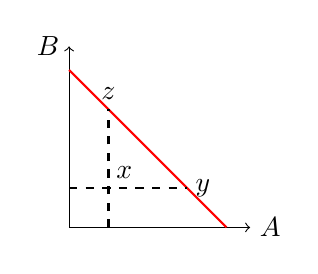
\begin{tikzpicture}
 \draw [->] (0, 0) -- (2.3, 0) node [right] {$A$};
 \draw [->] (0, 0) -- (0, 2.3) node [left] {$B$};
 \draw [red, thick] (0, 2) -- (2, 0);
 \draw [dashed, thick] (0, 0.5) -- (1.5, 0.5);
 \draw [dashed, thick] (0.5, 0) -- (0.5, 1.5);
 \node at (0.7,0.7) {$x$};
 \node at (0.5,1.7) {$z$};
 \node at (1.7,0.5) {$y$};
 \end{tikzpicture}
\end{center}\vspace*{-1ex}
\begin{itemize}
	\item Given an initial situation, a \emph{Pareto improvement} is a new situation where some agents will gain, and no agents will lose.
	\item A situation is called \emph{Pareto dominated} iff it has a Pareto improvement.
	\item A situation is called \emph{Pareto optimal} iff no change could lead to improved satisfaction for some agent without some other agent losing.
	\item The \emph{Pareto frontier} is the set of all Pareto optimal allocations.
\end{itemize}
\begin{table}
\begin{tabu}{c|c}
\hline
not change & change\\
\hline
$100,100$ & $1000,99$\\
\hline
\end{tabu}\caption{Pareto Improvement vs Rawls' Fair Opportunity Principle (veil of ignorance)}
$0.5*1000+0.5*90=545>100$
\end{table}
\end{frame}

\begin{frame}\frametitle{Rawls' Veil of Ignorance}
\begin{figure}[H]
\includegraphics[height=.35\textwidth]{img/veil-of-ignorance.png}
\includegraphics[height=.35\textwidth]{img/rawls.jpg}\caption{The reason that the least well off member gets benefited is that it is argued that under the veil of ignorance people will act as if they were risk-averse.}
\end{figure}
\begin{enumerate}
	\item Each citizen is guaranteed a fully adequate scheme of basic liberties, which is compatible with the same scheme of liberties for all others;
	\item Social and economic inequalities must satisfy two conditions:
	\begin{itemize}
		\item to the greatest benefit of the least advantaged (the difference principle);
		\item attached to positions and offices open to all.
	\end{itemize}
\end{enumerate}
\end{frame}

\begin{frame}\frametitle{}
\begin{itemize}
	\item Pessimism: Maximin rule (Rawls)
	\[
\abovetabulinesep=1mm
\belowtabulinesep=1mm
	\begin{tabu}{c|c|c|c|c}
		\hline
		& S_1 & S_2 & S_3 & S_4 \\
		\hline
		A_1 & 15 & \textcolor{red}{0} & \textcolor{red}{0} & 2 \\
		A_2 & \textcolor{red}{-1} & 4 & 3 & 7 \\
		A_3 & 6 & 4 & 14 & \textcolor{red}{1} \\
		\textcolor{red}{A_4} & 5 & 6 & 4 & \textcolor{red}{3} \\
		\hline
	\end{tabu}
	\]
	\item Optimisim: Maximax rule
	\item Optimisim-Pessimism rule
	\[\alpha \operatorname{Max}+(1-\alpha)\operatorname{Min}\]
	\item Expected utility maximization (utilitarianism)
	\item Minimax regret rule
\end{itemize}
\textbf{Remarks:} requires interpersonal comparison of utility.
\end{frame}

\begin{frame}\frametitle{Example}
\[
\abovetabulinesep=1mm
\belowtabulinesep=1mm
\begin{tabu}{c|c|c|c|c|c|c}
\hline
 & S_1 & S_2 & S_3 & \text{maximin} & \text{minimax regret} & \text{optimisim-pessimism}\atop \alpha=0.5 \\
\hline
A_1 & 1_{\textcolor{green}{0}} & 14_{\textcolor{green}{6}} & 13_{\textcolor{green}{0}} & \textcolor{red}{1} & \textcolor{green}{0} & 7.5 \\
A_2 & -1_{\textcolor{green}{2}} & 17_{\textcolor{green}{3}} & 11_{\textcolor{green}{2}} & -1 & \textcolor{red}{2} & 8 \\
A_3 & 0_{\textcolor{green}{1}} & 20_{\textcolor{green}{0}} & 6_{\textcolor{green}{7}} & 0 & \textcolor{green}{0} & \textcolor{red}{10} \\
\hline
\end{tabu}
\]
\end{frame}

\begin{frame}\frametitle{Example}
\begin{itemize}
	\item Two societies. $1000$ people. $100$ workers.
	\item The workers each receive $1$ unit of utility while the others get $90$ units each.
	\item The average utility is $10\%\cdot 1+90\%\cdot 90=81.1$
	\item In the second society, everyone take a fair turn at being a worker. This causes everyone to realize the same utility of $35$ units.
	\item The everage utility is $100\%\cdot 35$.
	\item The utilitarianism would count the first society as more just, but Rawls would favor the second.
\end{itemize}
\end{frame}

\begin{frame}\frametitle{卡尔多-希克斯(Kaldor-Hicks)标准}
\begin{block}{卡尔多-希克斯(Kaldor-Hicks)标准}
如果一种变革使得受益者的所得足以弥补受损者的所失,这种变革就是一个卡尔多-希克斯改进。如果受损者得到足够的补偿,就是帕累托改进。
\end{block}
\begin{itemize}
	\item 一家化工厂与家属区一墙之隔,为了上班方便,居民在化工厂的墙上挖了一个洞。一天,家属区的一个小孩钻洞进工厂玩,找到一瓶化学液体并点燃烧伤了自己。
	\item 假设化工厂补墙成本为$c$,如果不补墙,发生事故的概率为$p$,损失为$l$,且$c<pl$,化工厂需要承担责任吗?
\end{itemize}
\end{frame}

\begin{frame}\frametitle{外部性与科斯定理}
\begin{itemize}
	\item 个人收益与社会收益:一项活动的社会收益等于决策者个人得到的收益加社会其他成员得到的收益(如养花);
	\item 个人成本与社会成本:社会成本等于决策者的个人承担的成本加社会其他成员承担的成本(如环境污染、交通堵塞);
	\item 如果个人收益(成本)不等于社会收益,就存在外部性。
	\item 个人最优与社会最优的不一致意味着有帕累托改进的余地;
	\item 如何将外部性内部化?如何使得个人在边际上承担全部的社会成本、获得全部的社会收益?
	\item 政府征税或补贴?
	\item 科斯定理:只要产权界定是清楚的,如果交易成本为零,外部性可以通过当事人之间谈判解决,帕累托最优可以实现;并且,最终的资源配置与初始的产权安排无关。
\end{itemize}
\end{frame}

\begin{frame}\frametitle{科斯定理 --- 例子}
\begin{center}
 \begin{tikzpicture}
 \draw [->] (0, 0) -- (4.5, 0) node [right] {牧羊量};
 \draw [->] (0, 0) -- (0, 2.5) node [left] {};
 \draw [red, thick] (0, 2) -- (4, 0);
 \draw [red, thick] (0, 0) -- (4, 2);
 \draw [dashed, thick] (0, 1) -- (2, 1);
 \draw [dashed, thick] (2, 0) -- (2, 1);
 \node at (2,-0.2) {$S$};
 \node at (2,-0.6) {社会最优量};
 \node at (4,-0.2) {$P$};
 \node at (4.3,0.6) {牧羊的边际利润};
 \node at (3.7,1.6) {农场主的边际损失};
 \end{tikzpicture}
\end{center}
\begin{itemize}
	\item 如果产权归农场主,农场主禁止放牧,小于社会最优量$S$;但是,增加放牧给牧羊人带来的边际利润大于给农场主造成的损失,牧羊人将有积极性贿赂农场主,直到放牧量达到$S$为止;
	\item 如果产权归牧羊人,牧羊人的利润最大点是$P$,大于社会最优量$S$;但是,减少放牧量对牧羊人的边际利润损失小于给农场主节约的边际成本,农场主将有积极性贿赂牧羊人,直到放牧量达到$S$为止。
\end{itemize}
\end{frame}

\begin{frame}\frametitle{沉默的目击者}
\setlength\abovedisplayskip{0pt}
\setlength\belowdisplayskip{0pt}
\begin{itemize}
	\item $n$个目击者围观Kitty被虐杀。
	\item 报警的成本是$c$。
	\item 如果有人报警,Kitty会得救,每个目击者会获得效用$v$。如果没有人报警,目击者的效用是$0$。
\end{itemize}
\begin{table}
\begin{tabu}{c|c|c}
\hline
	& 报警 & 不报警 \\
\hline
报警 & $v-c,v-c$ & $v-c,v$ \\
不报警 & $v,v-c$ & $0,0$ \\
\hline
\end{tabu}
\end{table}
\begin{itemize}
	\item 当$v<c$时,所有人不报警是纳什均衡。
	\item 当$v>c$时,有一个人报警、其他人不报警是纳什均衡。
	\item 考虑对称的混合纳什均衡,即所有参与⼈报警的概率相等,设为$p$。此时,报警与不报警的期望收益相等。
	\[v-c=v(1-(1-p)^{n-1})\implies p=1-\left(\frac{c}{v}\right)^\frac{1}{n-1}\]
	\item $n$个人中至少有一人报警的概率为
	\[P(n)\coloneqq 1-(1-p)^n=1-\left(\frac{c}{v}\right)^\frac{n}{n-1}\]
	但$\frac{\mathrm{d}P(n)}{\mathrm{d}n}<0$,随着人数的增多,至少有一个人报警的概率下降。
\end{itemize}
\end{frame}

\begin{frame}\frametitle{走出囚徒困境 --- 奖惩 --- 利维坦}
\begin{table}
\abovetabulinesep=1mm
\belowtabulinesep=1mm
\begin{tabu}{c|cc}
\hline
 & cooperate & defect\\
\hline
Cooperate & $-1,-1$ & $-4,0$\\
Defect & $0,-4$ &\textcolor{yellow}{$-3,-3$}\\
\hline
\end{tabu}\caption{Prisoner's Dilemma}
\end{table}
\begin{table}
\abovetabulinesep=1mm
\belowtabulinesep=1mm
\begin{tabu}{c|cc}
\hline
 & cooperate & defect\\
\hline
Cooperate & $\textcolor{yellow}{-1,-1}$ & $-4,0-x$\\
Defect & $0-x,-4$ &$-3-x,-3-x$\\
\hline
\end{tabu}\caption{Prisoner's Dilemma with Punishment $0-x<-1$}
\end{table}	
\end{frame}

\begin{frame}\frametitle{走出囚徒困境 --- 奖惩 --- 作为激励机制的等级制度}
\begin{table}
\begin{tabu}{c|cc}
\hline
 & cooperate & defect\\
\hline
Cooperate & $3,3$ & $-1,4$\\
Defect & $4,-1$ & $0,0$\\
\hline
\end{tabu}
\[\MapDown{}\]
\begin{tabu}{c|cc}
\hline
 & first & second\\
\hline
First & $0,0$ & $2,1$\\
Second & $1,2$ & $0,0$\\
\hline
\end{tabu}
\end{table}
\begin{block}{儒家 --- “礼”}
“合作”方可得“君子”名分,君子享有优先权。\\
协调预期、定分止争。\\
声誉约束。
\end{block}
\end{frame}

\begin{frame}\frametitle{Multiple Nash Equilibria}
\begin{table}
\abovetabulinesep=1mm
\belowtabulinesep=1mm
\begin{tabu}{c|cc}
\hline
 & left & right\\
\hline
Left & \textcolor{yellow}{$1,1$} & $0,0$\\
Right & $0,0$ & \textcolor{yellow}{$1,1$}\\
\hline
\end{tabu}\caption{Coordination Game}
\end{table}
\begin{table}
\abovetabulinesep=1mm
\belowtabulinesep=1mm
\begin{tabu}{c|cc}
\hline
 & wcdma & td-scdma\\
\hline
WCDMA & \textcolor{green}{$8,8$} & $3,2$\\
TD-SCDMA & $2,3$ & \textcolor{yellow}{$4,4$}\\
\hline
\end{tabu}\caption{协商选择帕累托最优的纳什均衡}
\end{table}
\end{frame}

\begin{frame}\frametitle{Mixed Nash Equilibrium}
\begin{table}
\abovetabulinesep=1mm
\belowtabulinesep=1mm
\begin{tabu}{c|c|c}
\hline
 & 偷懒 & 不偷懒 \\
\hline
监督 & $1,-1$ & $-1,2$ \\
不监督 & $-2,3$ & $2,2$ \\
\hline
\end{tabu}
\end{table}
\begin{itemize}
	\item 如果员工偷懒的概率是$p$,那么,老板监督和不监督的期望收益分别为
	\[1\cdot p+(-1)\cdot(1-p)=2p-1\]
	\[(-2)\cdot p+2\cdot(1-p)=2-4p\]
	\item 如果老板监督的概率是$q$,那么,员工偷懒和不偷懒的期望收益分别为
	\[(-1)\cdot q+3\cdot(1-q)=3-4q\]
	\[2\cdot q+2\cdot(1-q)=2\]
	\item 混合纳什均衡是$(\frac{1}{4},\frac{1}{2})$,老板以$\frac{1}{4}$的概率监督,员工以$\frac{1}{2}$的概率偷懒。
\end{itemize}
\end{frame}

\begin{frame}\frametitle{承诺}
\begin{figure}[H]
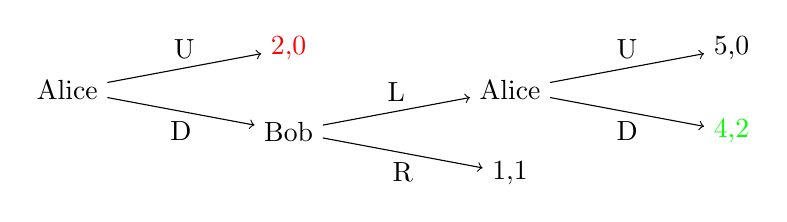
\begin{tikzpicture}[->,sibling distance=3em, level distance=8em, every node/.style={align=center},grow=right]
\node{Alice}
	child{node{Bob}
		child{node{1,1}
			edge from parent node [below] {R}}
		child{node{Alice}
			child{node{\textcolor{green}{4,2}}
				edge from parent node [below] {D}}
			child{node{5,0}
				edge from parent node [above] {U}}
			edge from parent node [above] {L}}
		edge from parent node [below] {D}}
	child{node{\textcolor{red}{2,0}}
		edge from parent node [above] {U}};
\end{tikzpicture}\caption{如果Alice承诺不选择U}
\end{figure}\vspace*{-2ex}
\begin{columns}
\column{.6\textwidth}
假如企业一开始定价80,如果前两个消费者购买了,企业将有积极性在50的价格下向第三个顾客出售。预期到这一点,前两个顾客将不会购买。如果企业承诺,任何降价的差额将返还顾客,前两个顾客则会购买。
\column{.3\textwidth}
\begin{table}
\begin{tabu}{c|c|c}
\hline
产量 & 价格 & 收入 \\
\hline
1 & 100 & 100 \\
2 & 80 & 160 \\
3 & 50 & 150 \\
4 & 30 & 120\\
\hline
\end{tabu}
\end{table}
\end{columns}
\begin{itemize}
	\item 承诺意味着限制自己的自由:选择少反而对自己好。
	\item 为什么画家死了画会升值?
	\item 民主、法治是政府对人民的一种承诺。
	\item 民法“民不告、官不究”,而刑法实行“公诉制度”是一种承诺。
\end{itemize}
\end{frame}

\begin{frame}\frametitle{逆向选择 --- 劣币驱逐良币}
\begin{figure}[H]
\begin{tikzpicture}[->,level 1/.style={sibling distance=20mm},level 2/.style={sibling distance=10mm}, level distance=10em, every node/.style={align=center},grow=right]
\node[circle,draw,inner sep=1.5,label=left:{卖方}]{}
	child{node(1)[circle,draw,inner sep=1.5]{}
		child{node{$x,0$}
			edge from parent node [below] {不买}}
		child{node{$Q,ax-Q$}
			edge from parent node [above] {买}}
		edge from parent node [below] {坏车$1-p$}}
	child{node(2)[circle,draw,inner sep=1.5]{}
		child{node{$2x,0$}
			edge from parent node [below] {不买}}
		child{node{$Q,2ax-Q$}
			edge from parent node [above] {买}}
		edge from parent node [above] {好车$p$}};
	\draw[dashed,rounded corners=10]($(1) + (-.5,-.3)$)rectangle($(2) + (.5,.3)$);
	\node at ($(1)!.5!(2)$){买方};
\end{tikzpicture}
\end{figure}
\begin{itemize}
	\item 假设好车和坏车对卖方的保留价值分别为$2x$和$x$,对买方的价值是卖方的$a$倍。成交价为$Q$。
	\item 为使交易达成,买方买车的期望收益应不小于不买车的期望收益。
	\[(2ax-Q)p+(ax-Q)(1-p)\geq 0\]
	\item 拥有好车的卖方能接受的最低价是$Q\geq 2x$。
	\item 这意味着,买卖双方合意的价格需满足:
	\[(1+p)ax\geq Q\geq 2x\implies p\geq\frac{2}{a}-1\]
\end{itemize}
\end{frame}

\begin{frame}\frametitle{如何解决非对称信息的问题?}
\begin{example}[逆向选择]
\begin{itemize}
	\item 坏车使得好车不能成交。
	\item 高风险的投保人使得低风险的投保人无法投保。
	\item 假乞丐使得真乞丐得不到救济。
	\item 高水平的学者竞争不过灌水的学者。
\end{itemize}
\end{example}
\begin{block}{解决非对称信息的市场机制和政府管制}
\begin{enumerate}
	\item 信号显示(signaling):卖方承诺保修。
	\item 信息甄别(screening):保险公司向投保人提供不同的合同选择,投保人根据自己的状况选择适合自己的合同。
	\item 声誉机制:品牌的价值。
	\item 适度的政府管制。但政府管制不当可能破坏声誉机制的有效性 --- 管制导致企业预期不稳定,追求短期行为;管制导致垄断,使得市场惩罚不可信;管制导致腐败,贿赂官员比贿赂投资者和客户更合算。
\end{enumerate}
\end{block}
\end{frame}

\begin{frame}\frametitle{Boxed Pig Game}
\begin{table}
\begin{tabu}{c|cc}
\hline
 & press & not press\\
\hline
Press & $4,0$ & $3,3$\\
Not Press & $7,-1$ & $0,0$\\
\hline
\end{tabu}\caption{Boxed Pig Game}
\end{table}
\begin{table}
\begin{tabu}{c|cc}
\hline
 & press & not press\\
\hline
Press & & $3,3$\\
Not Press & & $0,0$\\
\hline
\end{tabu}\caption{Rationalizability and Iterated Elimination of Dominated Actions}
\end{table}
\begin{table}
\begin{tabu}{c|cc}
\hline
 & press & not press\\
\hline
Press & & $3,3$\\
Not Press & &\\
\hline
\end{tabu}\caption{Rationalizability and Iterated Elimination of Dominated Actions}
\end{table}
\end{frame}

\begin{frame}\frametitle{\small Iterated Elimination of Dominated Actions and $n\textsuperscript{th}$-order Rationality}
\setlength\abovedisplayskip{0pt}
\setlength\belowdisplayskip{0pt}
\vspace*{-2ex}
\begin{table}
\[
\begin{tabu}{c|c|c|c|c}
\hline
 & c_1 & c_2 & c_3 & c_4 \\
\hline
r_1 & 5,10 & 0,11 & 1,20 & 10,10 \\
r_2 & 4,0 & \textcolor{red}{1,1} & 2,0 & 20,0 \\
r_3 & 3,2 & 0,4 & 4,3 & 50,1 \\
r_4 & 2,93 & 0,92 & 0,91 & 100,90 \\
\hline
\end{tabu}\qquad
\begin{tabu}{c|c|c|c}
\hline
 & c_1 & c_2 & c_3 \\
\hline
r_1 & 5,10 & 0,11 & 1,20 \\
r_2 & 4,0 & \textcolor{red}{1,1} & 2,0 \\
r_3 & 3,2 & 0,4 & 4,3 \\
r_4 & 2,93 & 0,92 & 0,91 \\
\hline
\end{tabu}
\]
\end{table}
\begin{table}
\[
\begin{tabu}{c|c|c|c}
\hline
 & c_1 & c_2 & c_3 \\
\hline
r_1 & 5,10 & 0,11 & 1,20 \\
r_2 & 4,0 & \textcolor{red}{1,1} & 2,0 \\
r_3 & 3,2 & 0,4 & 4,3 \\
\hline
\end{tabu}\qquad
\begin{tabu}{c|c|c}
\hline
 & c_2 & c_3 \\
\hline
r_1 & 0,11 & 1,20 \\
r_2 & \textcolor{red}{1,1} & 2,0 \\
r_3 & 0,4 & 4,3 \\
\hline
\end{tabu}\qquad
\begin{tabu}{c|c|c}
\hline
 & c_2 & c_3 \\
\hline
r_2 & \textcolor{red}{1,1} & 2,0 \\
r_3 & 0,4 & 4,3 \\
\hline
\end{tabu}
\]
\end{table}
\[
\begin{array}{lll}
	\text{0-order} & c_4\times & \operatorname{rational}(C)\\
	\text{1-order} & r_4\times & K_R \operatorname{rational}(C)\\
	\text{2-order} & c_1\times & K_CK_R \operatorname{rational}(C)\\
	\text{3-order} & r_1\times & K_RK_CK_R \operatorname{rational}(C)\\
	\text{4-order} & c_3\times & K_CK_RK_CK_R \operatorname{rational}(C)\\
	\text{5-order} & r_3\times & K_RK_CK_RK_CK_R \operatorname{rational}(C)
\end{array}
\]
\end{frame}

\begin{frame}\frametitle{风险与均衡}
\begin{itemize}
	\item 由于纳什均衡要求理性共识和一致预期,当人们可能犯小小的错误时,纳什均衡不一定被选择。
\end{itemize}
\begin{table}
\abovetabulinesep=1mm
\belowtabulinesep=1mm
\begin{tabu}{c|c|c}
\hline
 & left & right \\
\hline
up & \textcolor{red}{$8,10$} & $-1000,9$ \\
down & $7,6$ & $6,5$ \\
\hline
\end{tabu}\caption{只要B有千分之一的概率错误地选择right,A将选择down;如果B怀疑A怀疑自己可能犯错误,B将选择right。}
\end{table}
\end{frame}

\begin{frame}\frametitle{Infinitely Repeated Games}
\begin{table}
\begin{tabu}{c|cc}
\hline
 & cooperate & defect\\
\hline
Cooperate & $T,T$ & $S,R$\\
Defect & $R,S$ &\textcolor{yellow}{$P,P$}\\
\hline
\end{tabu}\caption{Prisoner's Dilemma: $R>T>P>S$ and $T+T > R+S$.}
\end{table}
\begin{enumerate}
	\item All-D策略:总是背叛。
	\item All-C策略:总是合作。
	\item 合作-背叛交替进行。
	\item 以牙还牙tit-for-tat TFT策略:从合作开始,之后每次选择对方前一阶段的行动。
	\item 冷酷grim策略:从合作开始,直到一方背叛,然后永远背叛。
	\item 宽容的冷酷策略:如果对方背叛,先惩罚几次,然后再恢复合作。
	\item 宽容的以牙还牙:永远以合作的态度来回报对方的合作。当遇到背叛时,以某一概率与对方进行合作。
	\item 赢定输移win stay, lose shift策略:如果我们上一轮合作,那么合作;如果上一轮都背叛,那么以一定概率合作;如果上一轮我合作你背叛或你合作我背叛,则背叛。
\end{enumerate}
\end{frame}

\begin{frame}\frametitle{}
\begin{itemize}
	\item $V(\operatorname{ALL-D},\operatorname{ALL-D})=P+\gamma P+\gamma^2 P+\dots=P\frac{1}{1-\gamma}$
	\item $V(\operatorname{TFT},\operatorname{TFT})=T+\gamma T+\gamma^2 T+\dots=T\frac{1}{1-\gamma}$
	\item $V(\operatorname{ALL-D},\textcolor{red}{\operatorname{TFT}})=R+\gamma P+\gamma^2 P+\dots=R+P\frac{\gamma}{1-\gamma}$
	\item $V(\operatorname{ALL-C},\textcolor{red}{\operatorname{grim}})=T+\gamma T+\gamma^2 T+\dots=T\frac{1}{1-\gamma}$
	\item $V(\operatorname{ALL-D},\textcolor{red}{\operatorname{grim}})=R+\gamma P+\gamma^2 P+\dots=R+P\frac{\gamma}{1-\gamma}$
\end{itemize}
如果$T\frac{1}{1-\gamma}\geq R+P\frac{\gamma}{1-\gamma}$,即$\gamma\geq\frac{R-T}{R-P}$,则对于grim策略来说,合作就是完美纳什均衡。
\end{frame}

\begin{frame}\frametitle{无名氏定理(Folk Theorem)}
在无限次重复博弈中,如果每个参与人都对未来足够重视(贴现因子足够大),那么,任何程度的合作都可以作为一个完美纳什均衡得到。这里的“合作程度”指整个博弈中合作出现的频率。
\end{frame}

\begin{frame}\frametitle{惩罚}
\begin{itemize}
	\item 在重复博弈中,越在乎长远利益,合作的可能性越大。
	\item 背叛行为越容易被观察到,并且惩罚越可信,合作的可能性越大。
	\item 垄断使得惩罚不可信。
	\item 在确定环境中,惩罚越严厉越有助于合作,但在不确定环境中,对方有可能是无心之失,冷酷策略可能不利于长期合作。
\end{itemize}
\begin{block}{联合抵制的社会规范}
Boycott(联合抵制):每个人都应该诚实;都有责任惩罚骗过人的人;不参与惩罚的人应该受到惩罚。
\end{block}
\textbf{Remark:} 朋友的朋友是朋友;朋友的敌人是敌人;敌人的朋友是敌人。
\end{frame}

\begin{frame}\frametitle{有限重复博弈}
\begin{table}
\abovetabulinesep=1mm
\belowtabulinesep=1mm
\[
\begin{tabu}{c|c|c|c}
\hline
 & c_1 & c_2 & c_3 \\
\hline
r_1 & \textcolor{red}{1,1} & 5,0 & 0,0 \\
r_2 & 0,5 & 4,4 & 0,0 \\
r_3 & 0,0 & 0,0 & \textcolor{red}{3,3} \\
\hline
\end{tabu}
\]
\end{table}
\begin{itemize}
	\item 两个纳什均衡:$(r_1,c_1)$和$(r_3,c_3)$
	\item 帕累托最优:$(r_2,c_2)$
	\item 如果博弈重复两次,则“好合好散,不欢而散”的策略 —— 如果$(r_2,c_2)$则$(r_3,c_3)$,否则$(r_1,c_1)$ —— 可在第一轮博弈中实现帕累托最优。
	\item 但是,如果第一轮遭到背叛后,第二轮对方重新谈判,则会使得惩罚不可信。原因在于多重均衡之间$(r_3,c_3)$帕累托优于$(r_1,c_1)$。
\end{itemize}
\end{frame}

\begin{frame}\frametitle{有限重复博弈}
\begin{table}
\[
\begin{tabu}{c|c|c|c|c|c}
\hline
 & c_1 & c_2 & c_3 & c_4 & c_5 \\
\hline
r_1 & \textcolor{red}{1,1} & 5,0 & 0,0 & 0,0 & 0,0 \\
r_2 & 0,5 & 4,4 & 0,0 & 0,0 & 0,0 \\
r_3 & 0,0 & 0,0 & \textcolor{red}{3,3} & 0,0 & 0,0 \\
r_4 & 0,0 & 0,0 & 0,0 & \textcolor{red}{4,0.5} & 0,0 \\
r_5 & 0,0 & 0,0 & 0,0 & 0,0 & \textcolor{red}{0.5,4} \\
\hline
\end{tabu}
\]
\end{table}
\begin{itemize}
	\item 四个纳什均衡:$(r_1,c_1)$、$(r_3,c_3)$、$(r_4,c_4)$、$(r_5,c_5)$
	\item 三个帕累托最优:$(r_2,c_2)$、$(r_4,c_4)$、$(r_5,c_5)$
	\item 如果博弈重复两次,则可采取如下策略:如果$(r_2,c_2)$则$(r_3,c_3)$;否则,被背叛的一方根据自己的情况选择$r_4$或$c_5$,如果双方同时背叛,则$(r_3,c_3)$。
	\item 此时惩罚变得可信了,均衡为:第一轮$(r_2,c_2)$;第二轮$(r_3,c_3)$。
\end{itemize}
\end{frame}

\begin{frame}\frametitle{单方不完全信息的有限重复博弈}
\begin{table}
\begin{tabu}{c|cc}
\hline
 & 合作 & 背叛\\
\hline
合作 & $3,3$ & $-1,4$\\
背叛 & $4,-1$ & $0,0$\\
\hline
\end{tabu}\qquad
\begin{tabu}{l|cc}
\hline
 & t1 & t2\\
\hline
A冷酷型$p$ & 合作 & $X$\\
A理性型$1-p$ & 背叛 & 背叛\\
\hline
B理性型 & $X$ & 背叛\\
\hline
\end{tabu}\caption{囚徒博弈重复两次}
\end{table}
\begin{itemize}
	\item 参与人A有两种可能的类型:“冷酷”型:选择grim策略,概率为$p$; “理性”型:可以选择任何策略,概率为$1-p$。
	\item 参与人B有一种类型:理性型。
	\item B在第一轮选择合作或背叛最后总的期望效用分别为
	\[3\cdot p+(-1)\cdot(1-p)+4\cdot p+0\cdot(1-p)=8p-1\]
	\[4\cdot p+0\cdot(1-p)+0\cdot p+0\cdot(1-p)=4p\]
	\item 如果$p\geq\frac{1}{4}$,则B在第一轮合作。
	\item 如果博弈重复$N\geq 3$轮,只要$p\geq\frac{1}{4}$,理性型A在$t=1\dots N-2$轮合作,在最后两轮背叛;B在前$N-1$轮合作,在最后一轮背叛。
\end{itemize}
\end{frame}

\begin{frame}\frametitle{双方不完全信息的有限重复博弈}
\begin{itemize}
	\item 假设双方都有两种可能的类型:“冷酷”型或“理性”型。
	\item 如果一开始就选择背叛,暴露了自己是理性型,那么收益最大为$4$。
	\item 假如对方采取冷酷策略的概率是$p$,则采取冷酷策略的最小期望收益为
	\[3\cdot N\cdot p+(-1+0+0+\dots+0)\cdot(1-p)=(3N+1)p-1\]
	\item 只要博弈次数$N\geq\frac{5-p}{3p}$,则采取冷酷策略。
	\item 在不完全信息的情况下,只要博弈重复的次数足够长,参与人就有积极性在博弈的早期建立一个“合作”的\textbf{声誉};一直到博弈的后期,才会选择背叛;并且,背叛的轮数只与$p$有关,而与博弈的次数$N$无关。
\end{itemize}
\end{frame}

\begin{frame}\frametitle{教育水平的信号传递作用}
\begin{itemize}
	\item 求职者$50\%$可能性是高能力者$50\%$可能性是低能力者。
	\item 高能力者的生产率是200,低能力者100。
	\item 雇主愿付高能力者工资200,低能力者100,不知道求职者能力高低则付平均工资150。
	\item 假设高能力者受教育成本40,低能力者受教育成本120。
	\item 此时,教育可以成为传递能力的信号。
	\item 但如果低能力者受教育的成本低于100,文凭就无法成为雇主区分能力高低的信号,雇主愿付的工资就是150,也就没人愿上大学了。
	\item 因此,关键是不同类型的人信号传递成本不同;只有成本差异足够大,才有可能传递信号。
\end{itemize}
\end{frame}

\begin{frame}\frametitle{Spence's Education Game}
\begin{itemize}
	\item The worker can be one of two types: wise $\theta_H$ (with probability $p$) or dumb $\theta_L$ (with probability $1-p$). Each type can select their own level of education, $e_H$ or $e_L$.
	\item The employer is assumed to have two choices. One is to ignore the signal and set $w^*\coloneqq p\theta_H+(1-p)\theta_L$. The other is to pay a worker $w_H$ or $w_L$ based on whether the signal is $e_H$ or $e_L$.
	\item The employer's payoff is $\theta-w$. The worker's payoff is $w-e/\theta$.
	\item This game has two equilibria. The first is a \textbf{pooling equilibrium}, in which the worker will choose the same level of education regardless of his type, and the employer pays all workers the same amount $w^*$.
	\item The other is a \textbf{separating equilibrium}, in which the worker will choose a different level of education. A low-talent worker will get no education, $e_L=0$. The education chosen by a high-talent worker is set in such a way as to make it unprofitable for either type of worker to mimic the other.
	\[w_L-0/\theta_L\geq w_H-e_H/\theta_L\quad\mbox{and}\quad w_H-e_H/\theta_H\geq w_L-0/\theta_H\]
\end{itemize}
\end{frame}

\begin{frame}\frametitle{信号传递的作用}
\begin{itemize}
	\item 为什么雄性孔雀的尾巴越长,越受到雌性孔雀的青睐?--- 只有健壮者才能负担得起长尾巴。
	\item 高、低质量产品哪个更愿意做广告?--- 广告费是高质量产品企业向市场传递信息的成本。
	\item 如何送礼?--- 重要的是送礼对送者的成本,而不是礼物对接受者的价值。
	\item 中秋为什么送浪费性的月饼?请客吃巨贵的馆子?--- 成本要高于价值,甚至“毁灭”了很大一部分价值更显出对对方的重视。“千里送鹅毛,礼轻仁义重。” 
	\item 公费请客送礼传递的信息量大打折扣,成本需要翻倍!
	\item 为什么领结婚证?--- 离婚分财产。同样,为什么送彩礼?为什么婚礼要铺张?
	\item 为什么街头古惑仔纹身?黑社会老大穿西装戴眼镜?
	\item 为什么很多繁文缛节没有实质意义的礼仪还要遵守?--- 合作精神
\end{itemize}
\end{frame}

\begin{frame}\frametitle{信息不完全导致社会规范变迁}
\begin{itemize}
	\item 如果是完全分离均衡,每类人的行为都是特定的。
	\item 如果是混同均衡,所有人的行为都是一样的。
	\item 如果是准分离(混同)均衡,有些行为传递信息,有些行为不传递信息。
	\item 如果外部因素导致社会由分离均衡转向混同均衡或准分离均衡,社会规范就会发生变化。
\end{itemize}
\begin{block}{}
人们对婚前性行为和婚外性行为态度的变化:在封闭的社会,婚前和婚外性行为都很容易观察;在流动的社会,有些能观察到,有些不能;如果被观察到的只是其中的一小部分,被观察到压力将会减少。
\end{block}
\end{frame}

\begin{frame}\frametitle{Auction}
\begin{enumerate}
	\item first-price open cry (English auction).
	\item dutch auction: (descending auction) the seller lowers the price until it is taken.
	\item first-price sealed bid: bidding without knowing the other bids.
	\item second-price sealed bid: (Vickrey auction) Highest bidder wins, but the price is the second highest bid!
\end{enumerate}
\begin{theorem}
Truth-telling is a dominant strategy in a second-price sealed bid.
\end{theorem}
\textbf{Remark:} 次价格密封拍卖的程序与高价格密封拍卖一样,中标者仍然是出价最高者,但中标者实际支付的是第二高报价。次价格密封拍卖能让竞标者有积极性说真话。
\end{frame}

\begin{frame}\frametitle{Vickrey-Clarke-Groves Mechanism}
\begin{itemize}
	\item 公共产品的偏好显示:不同的人有不同的偏好,是私人信息。如何让每个人报告自己的真实偏好?
	\item 每个人可以任意地报告自己的偏好,但可能要纳缴一定数量的“税”。计算办法:先将其他人的偏好加总,给出总价值最大的项目;然后将第一个人的偏好加上,如果不影响结果,不征税;否则,应纳税等于改变结果给其他人带来的损失。
	\item 比如同学聚会,选择哪个餐馆是一个公共产品。此机制可以让每人说出自己的真实偏好。
\end{itemize}
\begin{table}
\begin{tabu}{c|c|c|c}
\hline
	& 川菜 & 粤菜 & 税额 \\
\hline
A & 30 & 10 & 0 \\
B & 0 & 40 & 30 \\
C & 20 & 10 & 0 \\
\hline
合计 & 50 & 60 & 30\\
\hline
\end{tabu}
\end{table}
Truth-telling is the dominant strategy.
\end{frame}

\begin{frame}\frametitle{官员腐败问题}
\begin{itemize}
	\item $W$:官员工资。
	\item $B(q)$:权力租金,即官员在位置上可能收受的贿赂,也可看作不腐败的机会成本。一般来说,权力$q$越大,权力租金越高。
	\item $p$:腐败被发现的概率。
	\item $F$:对腐败的处罚。
	\item $U$:政府外的保留效用。
	\item $\alpha$:官员的羞耻感或脸皮厚度。
	\item 官员腐败的期望收益
	\[(1-p)(W+B(q))+p(U-\alpha F)\]
	\item 官员不腐败的条件:
	\[W\geq \frac{1-p}{p}B(q)+U-\alpha F\]
	\item 如何控制腐败?提高$p,F,W,\alpha$,减少$q$。
\end{itemize}
\end{frame}

\begin{frame}\frametitle{演化博弈 --- 婚姻博弈}
\begin{table}
\begin{tabu}{c|c|c}
\hline
& 物质型 & 感情型 \\
\hline
物质型 & $1,1$ & $0,0$ \\
感情型 & $0,0$ & $2,2$ \\
\hline
\end{tabu}
\end{table}
\begin{itemize}
	\item 假定总人口中,物质型的比例为$x$,感情型的比例为$1-x$。
	\item 对任何一个个体而言,物质型的期望效用:$x1+(1-x)0=x$。
	\item 感情型的期望效用:$x0+(1-x)2=2(1-x)$。
	\item 如果$x>2/3$,物质型更适合生存,将演化成稳定均衡。
	\item 如果$x<2/3$,感情型更适合生存,将演化成稳定均衡。
	\item 如果$x=2/3$,两类人有同样的适应性,但此二元均衡是非稳定的。
\end{itemize}
\end{frame}

\begin{frame}\frametitle{演化博弈 --- 鹰鸽博弈}
\begin{table}
\begin{tabu}{c|c|c}
\hline
& 鹰 & 鸽 \\
\hline
鹰 & $-1,-1$ & $1,0$ \\
鸽 & $0,1$ & $\frac{1}{2},\frac{1}{2}$ \\
\hline
\end{tabu}
\end{table}
\begin{itemize}
	\item 假定鹰派的比例是$x$,鸽派的比例是$1-x$。
	\item 鹰派的效用:$-1x+1(1-x)=1-2x$。
	\item 鸽派的效用:$0x+\frac{1}{2}(1-x)=\frac{1}{2}(1-x)$。
	\item 如果$x<1/3$,鹰派占优势,不稳定。
	\item 如果$x>1/3$,鸽派占优势,不稳定。
	\item 如果$x=1/3$,同样的适应性,稳定。
	\item 如果初始人口由单一类型构成,另一类型可以成功入侵,直到均衡。
\end{itemize}
\begin{itemize}
	\item[$\dagger$] 两个纯策略均衡:(鹰、鸽),(鸽、鹰);一个混合均衡:$(1/3,2/3)$
	\item[$\Delta$] 假定存在某种显性的标记机制:在博弈开始之前,每个人收到一个信号:A或B;概率是1/2;信号完全负相关;标记是公共知识。
\end{itemize}
\begin{enumerate}
	\item 如果A,选择“鹰”;如果B,选择“鸽”。是ESS。
	\item 如果A,选择“鸽”;如果B,选择“鹰”。是ESS。
	\item 无论AB,以1/3的概率选择“鹰”,2/3的概率选择“鸽”。不是ESS。
\end{enumerate}
\end{frame}

\begin{frame}\frametitle{}
\begin{definition}[Games in Extensive Form]
	A game in \emph{extensive form} $\Gamma=\langle N,\mathcal{A},\mathcal{H},\mathcal{Z},A,P,(\mathcal{I}_i)_{i\in N},f_c,(u_i)_{i\in N}\rangle$.
	\begin{itemize}
		\item The set of players $N$.
		\item The set of actions $\mathcal{A}\coloneqq\bigcup_{i\in N}\mathcal{A}_i$.
		\item A set $\mathcal{H}$ of sequences (finite or infinite) such that,
		\begin{enumerate}
			\item $\emptyset\in \mathcal{H}$
			\item $\forall m<n\left(h_{1:n}\in \mathcal{H}\implies h_{1:m}\in \mathcal{H}\right)$
			\item $\forall n\in\mathbb N\left(h_{1:n}\in \mathcal{H}\right)\implies h_{1:\infty}\in \mathcal{H}$
		\end{enumerate}
		\item A history $h\in \mathcal{H}$ is terminal iff $h=h_{1:\infty}$ or there is no $a\in \mathcal{A}$ s.t. $ha\in \mathcal{H}$. The set of terminal histories is denoted $\mathcal{Z}$.
		\item The set of actions at $h$: $A(h):=\{a:ha\in \mathcal{H}\}$.
		\item The player function: $P:\mathcal{H}\setminus \mathcal{Z}\to N\cup\{c\}$.
		\item The function $f_c$ associates with every history $h$ for which $P(h)=c$ a probability measure $f_c(\cdot\mid h)$ on $A(h)$. $f_c(\cdot\mid h)\in\Delta(A(h))$.
		\item For player $i\in N$, $\mathcal{I}_i\coloneqq \operatorname{Prt}(\{h\in \mathcal{H}:P(h)=i\})$ where $\forall h,h'\in I\in\mathcal{I}_i: A(h)=A(h^\prime)$.
		\item The Payoff function for each player $i\in N$: $u_i: \mathcal{Z}\to\mathbb R$.
	\end{itemize}
\end{definition}
\end{frame}

\begin{frame}\frametitle{}
\begin{itemize}
	\item If $|I|=1$ for all $I\in\mathcal{I}_i$ and all $i\in N$, then we say that $\Gamma$ is a game with \emph{perfect information}.
	\item If $|I|>1$ for some $i\in N$ and some $I\in\mathcal{I}_i$, then we say that $\Gamma$ is a game with \emph{imperfect information}.
	\item If all elements of $\Gamma$ are common knowledge, then we say that $\Gamma$ is a game with \emph{complete information}; otherwise, a game with \emph{incomplete information}.
\end{itemize}
\begin{theorem}
Every perfect information game in extensive form has a pure strategy Nash equilibrium.
\end{theorem}
\end{frame}

\begin{frame}\frametitle{Pure Strategy}
\begin{definition}[Pure Strategy]
	A \emph{pure strategy} of player $i$ is $s_i: \mathcal{I}_i\to \mathcal{A}$ s.t. $s_i(I)\in A(I)$ for all $I\in\mathcal{I}_i$.\\
	The \emph{set of pure strategies} of player $i$ is denoted by $S_i\coloneqq \prod\limits_{I\in\mathcal{I}_i}s_i(I)$.\\
	A \emph{strategy profile} \[s=(s_i)_{i\in N}\] is a vector consisting of one pure strategy for each player.\\
	The \emph{set of strategy profiles} is \[S=\prod\limits_{i\in N} S_i\]
	\[s_{-i}\coloneqq (s_1\ldots s_{i-1};s_{i+1}\ldots s_{|N|})\]
	\[S_{-i}\coloneqq S_1\times\ldots\times S_{i-1}\times S_{i+1}\times\ldots\times S_{|N|}\]
\end{definition}
\end{frame}

\begin{frame}\frametitle{}
\begin{definition}[Pure Strategy Consistent with History]
	For any history $h$ define a pure strategy $s_i$ of player $i$ to be consistent with $h$
	\[s_i\leadsto h\iff\forall k<\ell(h)\left(P(h_{1:k})=i\implies s_i(h_{1:k})=h_{k+1}\right)\]
\end{definition}
\[\sigma_c(h)\coloneqq \prod\limits_{h^\prime\sqsubseteq h}f_{P(h^\prime)}(h_{\ell(h^\prime)+1}\mid h^\prime)\]
where $f_{P(h)}(\cdot\mid h)\coloneqq 1$ if $P(h)\neq c$.\\
Each strategy profile $s=(s_i)_{i\in N}$ can be assigned a payoff for each player $i$:
\[u_i(s)\coloneqq \sum\limits_{h: \forall i(s_i\leadsto h)}\sigma_c(h)u_i(h)\]
Obviously, \[\forall h\in\mathcal{H}\left(P(h)\neq c\right)\implies u_i(s)=u_i(h^s)\] where $h^s$ is the history uniquely determined by $s$.
\end{frame}

\begin{frame}\frametitle{Mixed Strategy}
\setlength\abovedisplayskip{0pt}
%\setlength\belowdisplayskip{0pt}
\begin{definition}[Mixed Strategy]
	A \emph{mixed strategy} of player $i$ in an extensive game is a probability measure over the set of player $i$'s pure strategies:
	\[\sigma_i\in\Delta S_i\]
	A \emph{mixed strategy profile} specifies a mixed strategy for each	player $i$
	\[\sigma\coloneqq (\sigma_i)_{i\in N}\]
	The \emph{set of mixed strategy profiles} is:
	\[\prod\limits_{i\in N}\Delta S_i\]
	Each mixed strategy profile $\sigma=(\sigma_i)_{i\in N}$ implies a probability distribution
	over the \emph{set of pure strategy profiles} $S$
	\[\sigma(s)\coloneqq \prod\limits_{i\in N} \sigma_i(s_i)\]
\end{definition}
\end{frame}

\begin{frame}\frametitle{Payoff of Mixed Strategy}
\begin{definition}[Payoff of Mixed Strategy]
	The expected payoff of player $i$ given a mixed strategy profile $\sigma$ is
	\[u_i(\sigma)\coloneqq \sum\limits_{s\in S}u_i(s)\sigma(s)\]
\end{definition}
\end{frame}

\begin{frame}\frametitle{Behavioural Strategy}
\setlength\abovedisplayskip{0pt}
\begin{definition}[Behavioural Strategy]
	A \emph{behavioural strategy} of player $i$ is a collection $(\rho_i(I))_{I\in\mathcal{I}_i}$ of probability measures, where \[\rho_i(I)\in\Delta(A(I))\;\;\text{for $I\in\mathcal{I}_i$}\]
	A \emph{behavioural strategy profile} is a vector consisting of one	behavioural strategy for each player:
	\[\rho\coloneqq \left((\rho_i(I))_{I\in\mathcal{I}_i}\right)_{i\in N}\]
	For any history $h\in I\in\mathcal{I}_i$ and action $a\in A(h)$, we denote by $\rho_i(h)(a)$ the probability $\rho_i(I)(a)$ assigned by $\rho_i(I)$ to the action $a$.\\
	The \emph{set of behavioural strategies} of player $i$ is
	\[B_i\coloneqq \prod\limits_{I\in\mathcal{I}_i}\Delta(A(I))\]
	The \emph{set of behavioural strategy profiles} is:
	\[B\coloneqq \prod\limits_{i\in N}B_i=\prod\limits_{I\in\mathcal{I}}\Delta(A(I))\]
\end{definition}
\end{frame}

\begin{frame}\frametitle{Payoff of Behavioural Strategy}
\begin{definition}[Payoff of Behavioural Strategy]
	The expected payoff of player $i$ given a behavioural strategy profile $\rho$ is
	\[u_i(\rho)\coloneqq \sum\limits_{s\in S}u_i(s)\prod\limits_{i\in N}\prod\limits_{I\in\mathcal{I}_i}\rho_i(I)(s_i(I))\]
\end{definition}
\end{frame}

\begin{frame}\frametitle{Perfect Recall}
\begin{definition}[Experience Record]
Given a history $h$ of an extensive game, \emph{experience record} $X_i(h)$ is the sequence consisting of information sets that player $i$ encounters in $h$ and the actions that player $i$ takes at them.
\end{definition}
\begin{definition}[Perfect Recall]
An extensive game has \emph{perfect recall} if for each player $i$, we have $X_i(h) = X_i(h')$ whenever $h,h'$ are in the same information set of player $i$.
\end{definition}
\end{frame}

\begin{frame}\frametitle{Imperfect Recall}
\begin{figure}[H]
\begin{tikzpicture}[->,level 1/.style={sibling distance=16mm},level 2/.style={sibling distance=8mm}, level distance=8em, every node/.style={align=center},grow=right]
\node(1)[circle,draw,inner sep=1.5,label=left:{player1}]{}
	child{node(3)[circle,draw,inner sep=1.5]{}
		child{node{}
			edge from parent node [below] {}}
		child{node{}
			edge from parent node [above] {}}
		edge from parent node [below] {L}}
	child{node(2)[circle,draw,inner sep=1.5]{}
		child{node{}
			edge from parent node [below] {}}
		child{node{}
			edge from parent node [above] {}}
		edge from parent node [above] {R}};
	\draw[dashed,rounded corners=10]($(2) + (-.6,0.2)$)rectangle($(3) + (.6,-0.2)$);
	\node at ($(2)!.5!(3)$){player1};
\end{tikzpicture}\caption{$X_1(L)=\{\emptyset,L,\{L,R\}\},X_1(R)=\{\emptyset,R,\{L,R\}\}$}
\end{figure}
\begin{figure}[H]
\begin{tikzpicture}[->,level 1/.style={sibling distance=16mm},level 2/.style={sibling distance=8mm}, level distance=8em, every node/.style={align=center},grow=right]
\node(1)[circle,draw,inner sep=1.5,label=left:{}]{}
	child{node(3)[circle,draw,inner sep=1.5]{}
		child{node{1,0}
			edge from parent node [below] {L}}
		child{node{7,7}
			edge from parent node [above] {R}}
		edge from parent node [below] {L}}
	child{node(2)[circle,draw,inner sep=1.5]{}
		child{node{5,1}
			edge from parent node [below] {U}}
		child{node{2,2}
			edge from parent node [above] {D}}
		edge from parent node [above] {R}};
	\draw[dashed,bend right=70]($(1)$)to($(3)$);
	\node at ($(1)!.5!(2)-(0.1,1.9)$){player1};
	\node at ($(2)+(0,0.3)$){player2};
\end{tikzpicture}\caption{$X_1(\emptyset)=\{\{\emptyset,L\}\},X_1(L)=\{\{\emptyset,L\},L,\{\emptyset,L\}\}$}
\end{figure}
\end{frame}

\begin{frame}\frametitle{The difference between mixed and behavioral strategies}
\begin{figure}[H]
\begin{tikzpicture}[->,level 1/.style={sibling distance=16mm},level 2/.style={sibling distance=8mm}, level distance=8em, every node/.style={align=center},grow=right]
\node(1)[circle,draw,inner sep=1.5,label=left:{player1}]{}
	child{node(3)[circle,draw,inner sep=1.5]{}
		child{node{}
			edge from parent node [below] {A}}
		child{node{}
			edge from parent node [above] {B}}
		edge from parent node [below] {L}}
	child{node(2)[circle,draw,inner sep=1.5]{}
		child{node{}
			edge from parent node [below] {A}}
		child{node{}
			edge from parent node [above] {B}}
		edge from parent node [above] {R}};
	\draw[dashed,rounded corners=10]($(2) + (-.6,0.2)$)rectangle($(3) + (.6,-0.2)$);
	\node at ($(2)!.5!(3)$){player1};
\end{tikzpicture}
\end{figure}
\begin{itemize}
	\item Mixed strategies: $(p_{LA},p_{LB},p_{RA},p_{RB})$, for example, $(\frac{1}{2},0,0,\frac{1}{2})$
	\item Behavioral strategies: $\rho_i(\emptyset)(L)=p,\rho_i(\emptyset)(R)=1-p;\rho_i(\{L,R\})(A)=q,\rho_i(\{L,R\})(B)=1-q$.
\end{itemize}
\end{frame}

\begin{frame}\frametitle{Outcome-Equivalence}
For any profile $\sigma/\rho$, we define the \emph{outcome} $\overline{\sigma}(h)/\overline{\rho}(h)$ to be the multiplicative product of all the chance probabilities and move probabilities over history $h$ when all players choose their moves according to $\sigma_i/\rho_i$.
\[\sigma_i(h)\coloneqq \sum\limits_{s_i\leadsto h}\sigma_i(s_i)\]
\[\overline{\sigma}(h)\coloneqq \prod\limits_{i\in N\cup\{c\}}\sigma_i(h)\]
\[\overline{\rho}(h)\coloneqq \prod\limits_{k=0}^{\ell(h)}\rho_{P(h_{<k})}(h_{<k})(h_k)\sigma_c(h)\]
Two (mixed or behavioural) strategies of any player are \emph{outcome-equivalent} iff for every collection of pure strategies of the other players the two strategies induce the same outcome.
\begin{theorem}[Outcome-Equivalent Theorem]
	In games with perfect recall, for any mixed strategy there is an outcome-equivalent behavioural strategy and vice versa.
\end{theorem}
\end{frame}

\begin{frame}\frametitle{}
\begin{proof}
	``$\implies$''\\
	with perfect recall,
	\[\forall h,h^\prime\in I\in\mathcal{I}_i\forall a\in A(I)\left(\sigma_i(h)=\sigma_i(h^\prime)\implies\sigma_i(ha)=\sigma_i(h^\prime a)\right)\]
	\[\rho_i(I)(a)\coloneqq \dfrac{\sigma_i(ha)}{\sigma_i(h)}\;\;\text{for any $h\in I\in\mathcal{I}_i$}\]
	``$\impliedby$''
	\[\sigma_i(s_i)\coloneqq \prod\limits_{I\in\mathcal{I}_i}\rho_i(I)(s_i(I))\]
\end{proof}
\end{frame}

\begin{frame}\frametitle{Games in Strategic Form}
\begin{definition}[Strategy Form]
	A game in \emph{strategic form} is a triplet $\langle N,(S_i)_{i\in N},(u_i)_{i\in N}\rangle$.
	\begin{itemize}
		\item The sets of players $N$.
		\item The sets of strategies of the players $(S_i)_{i\in N}$.
		\item The payoff functions $u_i: S\to\mathbb R$.
	\end{itemize}
\end{definition}
\begin{definition}[Mixed Extension]
	The mixed extension of the strategic game $\langle N,(S_i)_{i\in N},(u_i)_{i\in N}\rangle$ is $\langle N,(\Delta S_i)_{i\in N},(u_i)_{i\in N}\rangle$, where the payoff function $u_i$ in $\langle N,(\Delta S_i)_{i\in N},(u_i)_{i\in N}\rangle$ is \[u_i(\sigma)=\sum\limits_{s\in S}u_i(s)\sigma(s)\]
\end{definition}
Note that $u_i$ is multilinear.
\[u_i(\lambda\sigma_i^\prime+(1-\lambda)\sigma_i^{\prime\prime};\sigma_{-i})=\lambda u_i(\sigma_i^\prime;\sigma_{-i})+(1-\lambda)u_i(\sigma_i^{\prime\prime};\sigma_{-i})\]
\end{frame}

\begin{frame}\frametitle{Moving between the Two Forms of Representation}
\begin{itemize}
	\item Each extensive form game can be represented in a unique way as a game in strategic form.
	\item There might be several games in extensive form which represent the same strategic form game.
	\item Games in strategic form can be interpreted as games in which all players choose simultaneously.
	\item Games in strategic form with two players and finite number of strategies can be represented by a matrix.
\end{itemize}
\end{frame}

\begin{frame}\frametitle{Translating from Extensive Form to Matrix Form}
\begin{figure}[H]
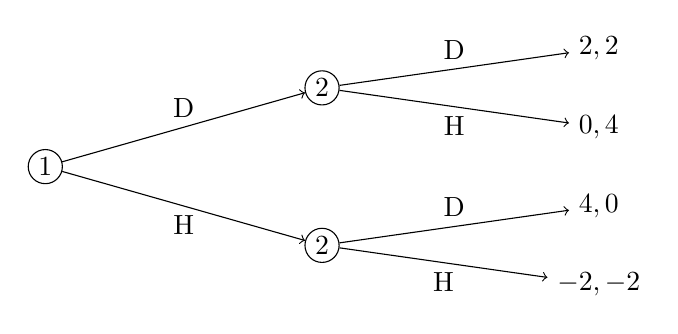
\begin{tikzpicture}[->,level 1/.style={sibling distance=20mm},level 2/.style={sibling distance=10mm}, level distance=10em, every node/.style={align=center},grow=right]
\node[circle,draw,inner sep=1.5]{1}
	child{node(1)[circle,draw,inner sep=1.5]{2}
		child{node{$-2,-2$}
			edge from parent node [below] {H}}
		child{node{$4,0$}
			edge from parent node [above] {D}}
		edge from parent node [below] {H}}
	child{node(2)[circle,draw,inner sep=1.5]{2}
		child{node{$0,4$}
			edge from parent node [below] {H}}
		child{node{$2,2$}
			edge from parent node [above] {D}}
		edge from parent node [above] {D}};
	%\draw[dashed,rounded corners=10]($(1) + (-.5,-.3)$)rectangle($(2) + (.5,.3)$);
\end{tikzpicture}\caption{The Hawk-Dove Game}
\end{figure}
\begin{table}
\[
\begin{tabu}{c|c|c|c|c}
\hline
 & (H|H,H|D) & (H|H,D|D) & (D|H,D|D) & (D|H,H|D) \\
\hline
H & -2,-2 & -2,-2 & 4,0 & 4,0 \\
D & 0,4 & 2,2 & 2,2 & 0,4 \\
\hline
\end{tabu}
\]
\end{table}
\end{frame}

\begin{frame}\frametitle{Pareto Optimality}
\begin{itemize}
	\item A strategy profile $s^*$ \emph{strongly Pareto-dominates} $s$ iff $\forall i\in N: u_i(s^*)>u_i(s)$.
	\item A strategy profile $s^*$ \emph{weakly Pareto-dominates} $s$ iff $\forall i\in N: u_i(s^*)\geq u_i(s)$ and $\exists i\in N: u_i(s^*)>u_i(s)$.
	\item A strategy profile $s^*$ is \emph{Pareto optimal} iff
	\[\forall i\in N\forall s\in S: u_i(s)>u_i(s^*)\implies\exists j\in N: u_j(s)<u_j(s^*)\]
\end{itemize}
\end{frame}

\begin{frame}\frametitle{Dominant Strategy Equilibrium}
\begin{definition}[Dominant Strategy]
	A strategy $s_i^*\in S_i$ is a \emph{dominant strategy} iff
	\[u_i(s_i^*;s_{-i})\geq u_i(s_i;s_{-i})\;\;\text{for all $s_i\in S_i$ and for all $s_{-i}\in S_{-i}$}\]
\end{definition}
\begin{definition}[Dominant Equilibrium]
	A strategy profile $s^*$ is a \emph{dominant strategy equilibrium} iff for each player $i\in N$, $s_i^*$ is a dominant strategy.
\end{definition}	
\end{frame}

\begin{frame}\frametitle{}
\begin{definition}[Strictly Dominated Strategy]
A strategy $s_i$ is called strictly dominated by $s_i'$ iff
\[\forall s_{-i}: u_i(s_i';s_{-i})>u_i(s_i;s_{-i})\]
\end{definition}
\begin{definition}[Weakly Dominated Strategy]
A strategy $s_i$ is called weakly dominated by $s_i'$ iff
\[\forall s_{-i}: u_i(s_i';s_{-i})\geq u_i(s_i;s_{-i})\]
and
\[\exists s_{-i}': u_i(s_i';s_{-i}')>u_i(s_i;s_{-i}')\]
\end{definition}
\begin{definition}[Iterated Dominance Equilibrium]
An \emph{iterated dominance equilibrium} is a strategy profile $s^*\in S$ obtained by iteratively ruling out dominated strategies from each player until only one strategy remains for each player.
\end{definition}
\end{frame}

\begin{frame}\frametitle{}
\begin{itemize}
	\item The result of iterative elimination of strictly dominated strategies is unique, i.e. independent of the elimination order.
	\item with weakly dominated strategies, the order of elimination matters.
\end{itemize}
\begin{table}
\[
\begin{tabu}{c|c|c|c}
\hline
 & c_1 & c_2 & c_3\\
\hline
r_1 & 1,1 & 0,1 & 3,1\\
r_2 & 1,0 & 2,2 & 1,3\\
r_3 & 1,3 & 3,1 & 2,2\\
\hline
\end{tabu}
\]
\end{table}
\begin{columns}
\column{0.2\textwidth}
\begin{enumerate}
	\item $r_2\times$
	\item $c_2\times$
	\item $r_3\times$
	\item $c_3\times$
	\item 
	$\begin{tabu}{c|c}
	\hline
	 & c_1\\
	\hline
	r_1 & 1,1\\
	\hline		
	\end{tabu}$
\end{enumerate}
\column{0.2\textwidth}
\begin{enumerate}
	\item $r_2\times$
	\item $c_2\times$; $c_3\times$
	\item 
	$\begin{tabu}{c|c}
	\hline
	 & c_1\\
	\hline
	r_1 & 1,1\\
	r_3 & 1,3\\
	\hline		
	\end{tabu}$
\end{enumerate}
\end{columns}
\end{frame}

\begin{frame}\frametitle{Nash Equilibrium}
\begin{definition}[Nash Equilibrium]
	\emph{Best response} of player $i$:
	\[\operatorname{BR}_i(s_{-i})\coloneqq \argmax\limits_{s_i\in S_i}u_i(s_i;s_{-i})\]
	
	The strategy profile $s^*$ is a \emph{Nash equilibrium} iff
	\[\forall i\in N: s_i^*\in\operatorname{BR}_i(s_{-i}^*)\]
\end{definition}
\begin{definition}[Mixed Nash Equilibrium]
	A mixed strategy profile $\sigma^*$ is a \emph{mixed Nash equilibrium} iff,
	\[\forall i\in N\forall\sigma_i\in\Delta S_i:\; u_i(\sigma_i^*;\sigma_{-i}^*)\geq u_i(\sigma_i;\sigma_{-i}^*)\]
\end{definition}
A mixed strategy Nash equilibrium of a strategic game is a Nash equilibrium of its mixed extension.
\end{frame}

\begin{frame}\frametitle{Kakutani Fixpoint Theorem}
\begin{theorem}[Kakutani Fixpoint Theorem]
Given a non-empty compact convex set $X\subset\mathbb{R}^n$ and a multi-valued function $f:X\rightrightarrows X$, if
\begin{enumerate}
	\item for all $x$, the set $f(x)$ is convex,
	\item for all sequences $(x_i,y_i)$ s.t. $x_i\in X$ and $y_i\in f(x_i)$,
	\[\lim_{i\to\infty}(x_i,y_i)=(x,y)\implies y\in f(x)\]
\end{enumerate}
then $\exists x\in f(x)$.
\end{theorem}
\begin{theorem}[Existence of Mixed Nash Equilibrium]
Every finite strategic game has a mixed Nash equilibrium.
\end{theorem}
\begin{proof}
Let $X\coloneqq\prod_{i\in N}\Delta S_i$ and $f(\sigma)\coloneqq\prod_{i\in N} \operatorname{BR}_i(\sigma_{-i})$.
\end{proof}
\end{frame}

\begin{frame}\frametitle{}
\begin{theorem}
	A mixed strategy profile $\sigma^*$ is a mixed Nash equilibrium iff,
	\[\forall i\in N\forall s_i\in S_i:\; u_i(\sigma_i^*;\sigma_{-i}^*)\geq u_i(s_i;\sigma_{-i}^*)\]
\end{theorem}
\begin{proof}
	\[u_i(\sigma_i;\sigma_{-i})=\sum\limits_{s_i\in S_i}u_i(s_i;\sigma_{-i})\sigma_i(s_i)\]
\end{proof}
\end{frame}

\begin{frame}\frametitle{}
\begin{theorem}
	For a finite strategic game,
	\[\operatorname{supp}(\sigma_i^*)\subset \operatorname{BR}_i(\sigma_{-i}^*)\]
\end{theorem}
\begin{proof}
	Suppose there exists an $s_i^\prime\in \operatorname{supp}(\sigma_i^*)$ s.t. \[u_i(s_i^\prime;\sigma_{-i}^*)<u_i(\sigma_i^*;\sigma_{-i}^*)\]
	then \[\sum\limits_{s_i\in S_i}u_i(s_i;\sigma_{-i}^*)\sigma_i^*(s_i)<u_i(\sigma_i^*;\sigma_{-i}^*)\]
	Contradiction!
\end{proof}
\end{frame}

\begin{frame}\frametitle{}
\begin{itemize}
	\item Every action in the support of any player's equilibrium mixed strategy yields that player the same payoff.
	\item If the set of actions of some player is not finite the result needs to be modified. In this case, $\sigma^*$ is a mixed strategy Nash equilibrium iff
	\begin{enumerate}
		\item for every player $i$ no action in $S_i$ yields, given $\sigma_{-i}^*$, a payoff to player $i$ that exceeds his equilibrium payoff, and
		\item the set of actions that yield, given $\sigma_{-i}^*$, a payoff less than his equilibrium payoff has $\sigma_i^*-$measure zero.
	\end{enumerate}
\end{itemize}
\end{frame}

\begin{frame}\frametitle{Maxmin Strategies}
\begin{itemize}
	\item The maxmin strategy for player $i$ is $\argmax\limits_{s_i}\min\limits_{s_{-i}}u_i(s_i;s_{-i})$, and player $i$'s maxmin value is $\max\limits_{s_i}\min\limits_{s_{-i}}u_i(s_i;s_{-i})$.
	\begin{itemize}
		\item Why would $i$ want to play a maxmin strategy?\item a conservative agent maximizing worst-case payoff.
	\end{itemize}
	\item In a two-player game, the minmax strategy for player $i$ against player $-i$ is $\argmin\limits_{s_i}\max\limits_{s_{-i}}u_{-i}(s_i;s_{-i})$, and player $-i$'s minmax value is $\min\limits_{s_i}\max\limits_{s_{-i}}u_{-i}(s_i;s_{-i})$.
	\begin{itemize}
		\item Why would $i$ want to play a minmax strategy?
		\item to punish the other agent as much as possible.
	\end{itemize}
\end{itemize}
\begin{theorem}[Minimax Theorem --- von Neumann 1928]
In any finite, two-player, zero-sum game, in any Nash equilibrium each player receives a payoff that is equal to both his maxmin value and his minmax value.
\end{theorem}
\end{frame}

\begin{frame}\frametitle{Imperfect Information Game}
\begin{figure}[H]
	\includegraphics[width=.5\textwidth]{img/poker.png}
\end{figure}
\end{frame}

\begin{frame}\frametitle{Counterfactual Regret Minimization}
Play a strategic game for a number of rounds:
\begin{itemize}
	\item Regret is determined after each game round: If I had played another move, my payoff would have been that much higher!
	\item Accumulate all positive regrets over time.
	\item Match the probabilities of a mixed strategy with the accumulated regret.
\end{itemize}
Take the average over all mixed strategies.
\begin{block}{}
If two players use the regret matching technique in a zero-sum game, then the average over the mixed strategies converges to Nash equilibrium strategies.
\end{block}
\end{frame}

\begin{frame}\frametitle{Counterfactual Regret Minimization}
\begin{itemize}
	\item The \textcolor{red}{reach probability} $\pi^\rho(h)\coloneqq\prod\limits_{i\in N\cup\{c\}}\pi_i^\rho(h)$ is the probability that history $h$ will be reached with strategy $\rho$, where $\pi_i^\rho$ is the contribution of player $i$, and $\pi_{-i}^\rho$ is the product of all player contributions except player $i$.
	\item $\pi^\rho(I)\coloneqq \sum\limits_{h\in I}\pi^\rho(h)$
	\item The \textcolor{red}{counterfactual reach probability} $\pi_{-i}^\rho(I)$ is the probability of reaching $I$ under the assumption that player $i$ always uses actions with probability $1$ in order to reach $I$.
	\item $\rho_{I\to a}$ is the same strategy as $\rho$, except that action $a$ is always chosen at information set $I$.
\end{itemize}
\end{frame}

\begin{frame}\frametitle{Counterfactual Regret Minimization}
\begin{itemize}
	\item The \textcolor{red}{counterfactual utility} of $\rho$ at non-terminal history $h$ is:
	\[v_i(\rho,h)\coloneqq \sum\limits_{z\in\mathcal{Z},h\sqsubset z}\pi_{-i}^\rho(h)\pi^\rho(z\mid h)u_i(z)\]
	\item The \textcolor{red}{counterfactual regret} of not taking action $a$ at history $h\in I$ is:
	\[r(h,a)\coloneqq v_i(\rho_{I\to a},h)-v_i(\rho,h)\]
	\item The \textcolor{red}{Counterfactual regret} of not taking $a$ at $I$ is:
	\[r(I,a)\coloneqq \sum\limits_{h\in I}r(h,a)\]
	\item $r_i^t(I,a)$ refers to the regret in episode $t$, when players use $\rho$ and player $i$ does not take $a$ at $I$.
	\item The \textcolor{red}{Cumulative counterfactual regret} is:
	\[R_i^T(I,a)\coloneqq \sum\limits_{t=1}^T r_i^t(I,a)\]
\end{itemize}
\end{frame}

\begin{frame}\frametitle{Counterfactual Regret Minimization}
\begin{itemize}
	\item The \textcolor{red}{positive cumulative counterfactual regret} is:
	\[R_i^{T,+}\coloneqq \max\left\{R_i^T(I,a),0\right\}\]
	\item The \textcolor{red}{regret matching strategy} for episode $T + 1$ is:
	\[\rho_i^{T+1}(I,a)\coloneqq
	\begin{cases}
		\frac{R_i^{T,+}(I,a)}{\sum\limits_{a\in A(I)}R_i^{T,+}(I,a)} &\mbox{if } \sum\limits_{a\in A(I)}R_i^{T,+}(I,a)>0\\
		\frac{1}{|A(I)|} &\mbox{otherwise}
	\end{cases}\]
	\item The \textcolor{red}{average strategy} is:
	\[\overline{\rho}_i^t(I)(a)\coloneqq\frac{\sum\limits_{t=1}^T\pi_i^{\rho^t}(I)\rho^t(I)(a)}{\sum\limits_{t=1}^T\pi_i^{\rho^t}(I)}\]
\end{itemize}
\end{frame}

\begin{frame}\frametitle{Regret Matching --- RPS example with two rounds}
Assume we play rock, paper, scissors, and player $1$ uses
regret matching.
\begin{enumerate}
	\item Initial cumulative regret is $(0,0,0)$
	\item Play uniform strategy $(\frac{1}{3},\frac{1}{3},\frac{1}{3})$
	\item Player $1$ chooses $R$, while player $2$ chooses $P$
	\item Regret for player $1$:
	\begin{itemize}
		\item $R: u_1(R,P)-u_1(R,P)=-1--1=0$
		\item $P: u_1(P,P)-u_1(R,P)=0--1=1$
		\item $S: u_1(S,P)-u_1(R,P)=1--1=2$
	\end{itemize}
	\item Player $1$'s cumulative counterfactual regret is now $(0,1,2)$
	\item Regret matching strategy: $\rho_1^1=(0,\frac{1}{3},\frac{2}{3})$
	\item Player $1$ chooses $P$, while player $2$ chooses $S$
	\item Regret for player $1$:
	\begin{itemize}
		\item $R: u_1(R,S)-u_1(P,S)=1--1=2$
		\item $P: u_1(P,S)-u_1(P,S)=-1--1=0$
		\item $S: u_1(S,S)-u_1(P,S)=0--1=1$
	\end{itemize}
	\item Player $1$'s cumulative counterfactual regret is now $(2,1,3)$
	\item Regret matching strategy: $\rho_1^2=(\frac{1}{3},\frac{1}{6},\frac{1}{2})$
\end{enumerate}
\end{frame}

\begin{frame}\frametitle{}
\begin{figure}
	\includegraphics[width=.35\textwidth]{img/rps.png}
\end{figure}
\begin{enumerate}\setcounter{enumi}{10}
	\item The average strategy: $(\frac{1}{6},\frac{1}{4},\frac{7}{12})$.\\
	Not close to NE, but will converge!
\end{enumerate}
\begin{columns}
\column{.3\textwidth}
\[
\begin{tabu}{c|ccc}
& R & P & S\\
\hline
t_0 & \frac{1}{3} & \frac{1}{3} & \frac{1}{3}\\
t_1 & 0 & \frac{1}{3} & \frac{2}{3} \\
t_2 & \frac{1}{3} & \frac{1}{6} & \frac{1}{2}\\
\end{tabu}
\]
\[h=RP\]
\column{.5\textwidth}
\begin{align*}
	\frac{\frac{1}{3}\times\frac{1}{3}\times 0 + \frac{1}{3}\times\frac{1}{3}\times\frac{1}{3}}{\frac{1}{3}\times\frac{1}{3}+\frac{1}{3}\times\frac{1}{3}}&=\frac{1}{6}\\
	\frac{\frac{1}{3}\times\frac{1}{3}\times\frac{1}{3} + \frac{1}{3}\times\frac{1}{3}\times\frac{1}{6}}{\frac{1}{3}\times\frac{1}{3}+\frac{1}{3}\times\frac{1}{3}}&=\frac{1}{4}\\
	\frac{\frac{1}{3}\times\frac{1}{3}\times\frac{2}{3} + \frac{1}{3}\times\frac{1}{3}\times\frac{1}{2}}{\frac{1}{3}\times\frac{1}{3}+\frac{1}{3}\times\frac{1}{3}}&=\frac{7}{12}
\end{align*}
\end{columns}
\end{frame}

\begin{frame}\frametitle{Trembling Hand Perfect Equilibrium}
\begin{definition}[Trembling Hand Perfect Equilibrium]
A strategy profile $\sigma$ is a \emph{trembling hand perfect equilibrium} iff there exists a sequence of completely mixed strategy profiles $\sigma^k\to\sigma$ such that $\forall i\forall k: \sigma_i\in \operatorname{BR}_i(\sigma_{-i}^k)$.
\end{definition}
\begin{theorem}
A strategy profile in a finite two-player strategic game is a trembling hand perfect equilibrium iff it is a mixed strategy Nash equilibrium and the strategy of neither player is weakly dominated.
\end{theorem}
\begin{theorem}
Every finite strategic game has a trembling hand perfect equilibrium.
\end{theorem}
\end{frame}

\begin{frame}\frametitle{}
Let $\Omega$ be the uncertainty space, $\mathcal{I}_i$ be the information partition of player $i$, $P(\cdot\mid\mathcal{I}_i)\in\Delta\Omega$ be the interim belief systems, and $v_i: \Omega \to S_i$ be measurable with regard to $\mathcal{I}_i$. Then $(v_i)_{i\in N}$ is a posteriori equilibrium of the strategic game $(N,S_i,u_i)$ if for all $i\in N$ and $s_i\in S_i$:
\[\sum_{\omega \in \Omega}P(\omega\mid\mathcal{I}_i(\omega))u_i(v_i(\omega ),v_{-i}(\omega))\geq\sum_{\omega \in \Omega}P(\omega\mid\mathcal{I}_i(\omega))u_i\left(s_i,v_{-i}(\omega)\right)\]
\end{frame}

\begin{frame}\frametitle{Subgame}
某个博弈的子博弈是由该博弈的某个单一结点(即该结点所在的信息集就只包含一个要素,就是该结点)及其所有后续结点构成的集合,并且所有的后续结点必须满足一个条件,即如果某一个后续结点属于该子博弈,那么该后续结点所在信息集的所有结点必须也属于该子博弈。
\begin{definition}[Subgame]
	The \emph{subgame} of the extensive game $\Gamma$ that follows the history $h$
	is the extensive game $\Gamma(h)\coloneqq \langle N,P|_h,\mathcal{H}|_h,(\mathcal{I}_i)_{i\in N},f_c,(u_i|_h)_{i\in N}\rangle$, where
	\[P|_h(h^\prime)\coloneqq P(hh^\prime)\]
	\[\mathcal{H}|_h\coloneqq \{h^\prime:hh^\prime\in\mathcal{H}\}\]
	\[u_i|_h(h^\prime)\coloneqq u_i(hh^\prime)\]
	\[\forall I\in\bigcup\limits_{i\in N}\mathcal{I}_i:\,I\subset\{hh^\prime:h^\prime\in\mathcal{H}|_h\}\;\vee\;I\subset\mathcal{H}\setminus \{hh^\prime:h^\prime\in\mathcal{H}|_h\}\]
\end{definition}	
\end{frame}

\begin{frame}\frametitle{Subgame Perfect Equilibrium}
\begin{definition}[Subgame Perfect Equilibrium]
	A \emph{subgame perfect equilibrium} of an extensive game $\Gamma$ is a strategy profile $s^*$ such that for every player $i\in N$ and every nonterminal history $h\in\mathcal{H}\setminus\mathcal{Z}$ for which $P(h)=i$ we have \[u_i|_h(s_i^*;s_{-i}^*)\geq u_i|_h(s_i;s_{-i}^*)\]
	for every strategy $s_i$ of player $i$ in the subgame $\Gamma(h)$.
	
	A behaviour strategy profile $\rho^*$ is a \emph{subgame perfect equilibrium} of a game $\Gamma$ iff for all subgames $\Gamma(h)$ of $\Gamma$, and,
	\[\forall i\in N\forall\rho_i\in B_i:\, u_i|_h(\rho_i^*;\rho_{-i}^*)\geq u_i|_h(\rho_i;\rho_{-i}^*)\]
\end{definition}
\begin{theorem}[Kuhn's Theorem]
Every finite extensive game has a subgame-perfect equilibrium.
\end{theorem}
\end{frame}

\begin{frame}[fragile]{\href{https://mp.weixin.qq.com/s/LLUoU0gl3t6GTh6jDef5vA}{Pirate Game}}
	\begin{problem}[\switchocg{ocg2}{Pirate Game}]
		\switchocg{ocg3}{$5$ rational pirates} have a treasure of 100 gold coins.\\
		The pirate world's rules of distribution are thus:
		\begin{enumerate}
			\item The fiercest pirate proposes how to split the coins, and all pirates (including the proposer) vote for or against it;
			\item If \switchocg{ocg4}{$50\%$ or more} of the pirates vote for it, then the coins will be shared that way. Otherwise, the proposer will be thrown overboard, and the procedure is repeated with the next fiercest pirate;
			\item As the pirates are bloodthirsty, each pirate would prefer to throw another overboard, if all other results would otherwise be equal.
		\end{enumerate}
	\end{problem}
\begin{ocg}{pirate1}{ocg2}{0}
\begin{verbatim}
1,0,1,0,98
\end{verbatim}
\end{ocg}
\begin{ocg}{pirate2}{ocg3}{0}
\begin{verbatim}
What about more than 200 pirates? Who can survive?
1-200, 201, 202, 204, 200+2^n
\end{verbatim}
\end{ocg}
\begin{ocg}{pirate3}{ocg4}{0}
\begin{verbatim}
What about more than half?
0,2,1,0,97 / 2,0,1,0,97
\end{verbatim}
\end{ocg}
\end{frame}

\begin{frame}\frametitle{Sequentially Rationality}
\begin{definition}[Assessment]
	An \emph{assessment} in an extensive game is a pair $(\rho,\mu)$, where $\rho$ is a profile of behavioural strategies and $\mu$ is a belief system. $\mu(I)(h)$ is the probability that player $P(I)$ assigns to the history $h\in I$, conditional on $I$ being reached.
\end{definition}
\begin{definition}[Sequentially Rationality]
	An assessment $(\rho,\mu)$ is \emph{sequentially rational} iff for every player $i$ and every information set $I\in\mathcal{I}_i$ the strategy of player $i$ is a best response to the other players' strategies given $i$'s beliefs at $I$.
	\[\forall\rho_i^\prime\in B_i:\, \sum\limits_{h\in I}u_i|_h(\rho_i;\rho_{-i})\mu(I)(h)\geq\sum\limits_{h\in I}u_i|_h(\rho_i^\prime;\rho_{-i})\mu(I)(h)\]
\end{definition}
\end{frame}

\begin{frame}\frametitle{}
We can define the outcome $O(\rho,\mu\mid I)$ as the distribution over terminal histories determined by $\rho$ and $\mu$ conditional on $I$ being reached.
\[
O(\rho,\mu\mid I)(h^\prime)\coloneqq 
\begin{cases}
0 &\text{if $\nexists h\in I\left(h\sqsubset h^\prime\right)$}\\
\mu(I)(h)\prod\limits_{k=\ell(h)}^{\ell(h^\prime)}\rho_{P(h_{<k})}(h_{<k})(h_k) &\text{otherwise}
\end{cases}
\]
since by perfect recall, there is at most one subhistory $h$ of $h^\prime$ in $I$, and the histories $h_{1:k}$ for $k=\ell(h),\ldots,\ell(h^\prime)$ lie in different information sets.
\end{frame}

\begin{frame}\frametitle{}
\begin{itemize}
	\item An assessment $(\rho,\mu)$ is \emph{sequentially rational} iff for every player $i$ and every information set $I\in\mathcal{I}_i$
\[\forall \rho_i^\prime\in B_i:\, O(\rho,\mu\mid I)\succcurlyeq_i O((\rho_i^\prime;\rho_{-i}),\mu\mid I)\]
	\item A behavioural strategy profile to be \emph{\emph{completely mixed}} iff it assigns positive probability to every action at every information set.
\end{itemize}
\end{frame}

\begin{frame}\frametitle{}
\begin{definition}[Consistency of Beliefs with Strategies]
	Let $\Gamma$ be a finite extensive game with perfect recall. An assessment $(\rho,\mu)$ is \emph{consistent} iff there is a sequence $((\rho^n,\mu^n))_{n=1}^\infty$ of assessments s.t. $(\rho,\mu)=\lim\limits_{n\to\infty}(\rho^n,\mu^n)$ and each strategy profile $\rho^n$ is completely mixed and each belief system $\mu^n$ is derived from $\rho^n$ using Bayes' rule: \[\mu^n(I)(h)=\dfrac{\overline{\rho}^n(h)}{\sum\limits_{h\in I}\overline{\rho}^n(h)}\]
\end{definition}
\end{frame}

\begin{frame}\frametitle{}
\begin{definition}[Sequential Equilibrium]
	An assessment is a \emph{sequential equilibrium} of a finite extensive game with perfect recall iff it is sequentially rational and consistent.
\end{definition}
\begin{theorem}
	Every finite extensive game with perfect recall has a sequential equilibrium.
\end{theorem}
\begin{theorem}
	In an extensive game with perfect information, $(\rho,\mu)$ is a sequential equilibrium iff $\rho$ is a subgame perfect equilibrium.
\end{theorem}
\end{frame}

\begin{frame}\frametitle{Bayesian Strategic Game with Observable Actions}
\begin{definition}[Bayesian Strategic Game with Observable Actions]
	A Bayesian game is a tuple $\langle N,(S_i)_{i\in N},(\Theta_i)_{i\in N},p,(u_i)_{i\in N}\rangle$ where
	\begin{itemize}
		\item The sets of players $N$.
		\item The sets of strategies of the players $(S_i)_{i\in N}$.
		\item $\Theta_i$ is a finite set (the set of possible types of player $i$). $\Theta\coloneqq \prod\limits_{i\in N}\Theta_i$.
		\item $p\in\Delta\Theta$.
		\item $u_i: S\times\Theta\to\mathbb R$
	\end{itemize}
\end{definition}
\end{frame}

\begin{frame}\frametitle{Expected Utility}
\begin{enumerate}
	\item ex-post --- the agent knows all agents' types.
	\item ex-interim --- an agent knows her own type but not the types of the other agents.
	\item ex-ante --- the agent knows nothing about anyone's actual type.
\end{enumerate}
\end{frame}

\begin{frame}\frametitle{Ex-post Expected Utility}
\begin{definition}[Ex-post Expected Utility]
	Player $i$'s ex post expected utility in a Bayesian game is defined as
	\[V_i(\sigma,\theta)\coloneqq \sum\limits_{s\in S}\left(\prod\limits_{j\in N}\sigma_j(s_j\mid\theta_j)\right)u_i(s,\theta)\]
	where the players' types are given by $\theta\in\Theta$, and the players' strategies are given by $\sigma\in\prod\limits_{i\in N}\prod\limits_{\theta_i\in\Theta_i}\Delta S_i$, $\sigma=(\sigma_i(\cdot\mid\theta_i))_{\theta_i\in\Theta_i,i\in N}$, $\sigma_i(\cdot\mid\theta_i)\in\Delta S_i$.
\end{definition}	
\end{frame}

\begin{frame}\frametitle{Ex-interim Expected Utility}
\begin{definition}[Ex-interim Expected Utility]
	Player $i$'s ex interim expected utility in a Bayesian game, where $i$'s type is $\theta_i$ and where the players' strategies are given by the mixed-strategy profile $\sigma$, is defined as
	\[V_i(\sigma,\theta_i)\coloneqq \sum\limits_{\theta_{-i}\in\Theta_{-i}}p(\theta_{-i}\mid\theta_i)\sum\limits_{s\in S}\left(\prod\limits_{j\in N}\sigma_j(s_j\mid\theta_j)\right)u_i(s,(\theta_i;\theta_{-i}))\]
	or equivalently as
	\[V_i(\sigma,\theta_i)=\sum\limits_{\theta_{-i}\in\Theta_{-i}}p(\theta_{-i}\mid\theta_i)V_i(\sigma,(\theta_i;\theta_{-i}))\]
\end{definition}
\end{frame}

\begin{frame}\frametitle{Ex-ante Expected Utility}
\begin{definition}[Ex-ante Expected Utility]
	Player $i$'s ex ante expected utility in a Bayesian game, where the players' strategies are given by the mixed-strategy profile $\sigma$, is defined as
	\[V_i(\sigma)\coloneqq \sum\limits_{\theta\in\Theta}p(\theta)\sum\limits_{s\in S}\left(\prod\limits_{j\in N}\sigma_j(s_j\mid\theta_j)\right)u_i(s,\theta)\]
	or equivalently as
	\[V_i(\sigma)=\sum\limits_{\theta\in\Theta}p(\theta)V_i(\sigma,\theta)\]
	or again equivalently as
	\[V_i(\sigma)=\sum\limits_{\theta_i\in\Theta_i}p(\theta_i)V_i(\sigma,\theta_i)\]
\end{definition}	
\end{frame}

\begin{frame}\frametitle{Best Response in a Bayesian Game}
\begin{definition}[Best Response in a Bayesian Game]
	The set of player $i$'s best response to mixed-strategy profile $\sigma_{-i}$ are given by
	\[\operatorname{BR}_i(\sigma_{-i})\coloneqq \argmax_{\sigma_i\in \Delta S_i^{\Theta_i}}V_i(\sigma_i;\sigma_{-i})\]
\end{definition}
\textbf{Remark:} It may seem odd that $\operatorname{BR}_i$ is calculated based on $i$'s ex ante expected utility. However, we are in fact performing independent maximization of $i$'s \emph{ex interim expected utilities} conditioned on each type that he could have.\\
Intuitively speaking, if a certain action is best after the signal is received, it is also the best conditional plan devised ahead of time for what to do should that signal be received.	
\end{frame}

\begin{frame}\frametitle{}
\begin{definition}[Bayesian Equilibrium]
	A Bayesian equilibrium is a mixed strategy profile $\sigma^*$ that satisfies
	\[\forall i\in N:\, \sigma_i^*\in \operatorname{BR}_i(\sigma_{-i}^*)\]
\end{definition}
\begin{definition}[Ex-post Equilibrium]
	An ex post equilibrium is a mixed strategy profile $\sigma$ that satisfies
	\[\forall\theta\in\Theta\forall i\in N:\, \sigma_i\in\argmax\limits_{\sigma_i\in\Delta S_i^{\Theta_i}}V_i((\sigma_i;\sigma_{-i}),\theta)\]
\end{definition}
The ex post equilibrium is similar in flavor to equilibria in dominant strategies, which do not require agents to believe that other agents act rationally. However, it seems too good to be true most of the time.
\end{frame}

\begin{frame}\frametitle{Bayesian Extensive Game with Observable Actions}
\begin{definition}[Bayesian Extensive Game with Observable Actions]
	A \emph{Bayesian extensive game with observable actions} is a tuple
	$\langle\Gamma,(\Theta_i)_{i\in N},(p_i)_{i\in N},(u_i)_{i\in N}\rangle$ where
	\begin{itemize}
		\item $\Gamma=\langle N,P,\mathcal{H}\rangle$ is an extensive game form with perfect information and simultaneous moves.
		\item $\Theta_i$ is a finite set (the set of possible types of player $i$). $\Theta\coloneqq \prod\limits_{i\in N}\Theta_i$.
		\item $p_i\in\Delta^0(\Theta_i)$.
		\item $u_i: \mathcal{H}\times\Theta\to\mathbb R$
	\end{itemize}
\end{definition}
\end{frame}

\begin{frame}\frametitle{}
\textbf{Remark:} the type of player encapsulates all the information possessed by the player that is not common knowledge. This is often quite simple (e.g. the player's knowledge of his private payoff function), but can also include his beliefs about other players' payoffs, about their beliefs about his own payoff, and any other higher-order beliefs.
\end{frame}

\begin{frame}\frametitle{}
There is a way of capturing the common prior is to hypothesize a special agent $c$ called ``Nature'' who makes probabilistic choices.
The agent ``nature''($c$) selects the types of the players, who are subsequently fully cognizant at all points of all moves taken previously. We can associate with any such game an extensive game (with imperfect information and simultaneous moves) in which the set of histories is $\{\emptyset\}\cup(\mathcal{H}\times\Theta)$ and each information set of each player $i$ takes the form
\[I(h,\theta_i)\coloneqq \{(h,(\theta_i,\theta_{-i})):\theta_{-i}\in\Theta_{-i}\}\]
for $i\in P(h)$ and $\theta_i\in\Theta_i$.
\end{frame}

\begin{frame}\frametitle{}
Let $s$ be a profile of behavioural strategies in $\Gamma$. Define $O_h(s)$ to be the probability measure on the set of terminal histories of $\Gamma$ generated by $s$ given that the history $h$ has occurred. Define $O((s_i;\rho_{-i}),\mu_{-i}\mid h)$ to be the probability measure on the set of terminal histories of $\Gamma$ given that player $i$ uses the strategy $s_i$ in $\Gamma$, each type $\theta_j$ of each player $j$ uses the strategy $\rho_j(\theta_j)$, the game has reached $h$, and
the probability that $i$ assigns to $\theta_{-i}$ is derived from $\mu_{-i}(h)$. That is, $O((s_i;\rho_{-i}),\mu_{-i}\mid h)$ is the compound lottery in which the probability of the lottery $O_h(s_i;(\rho_j(\theta_j))_{j\in N\setminus\{i\}})$ is $\prod\limits_{j\in N\setminus\{i\}}\mu_j(h)(\theta_j)$ for each $\theta_{-i}\in\Theta_{-i}$.
\end{frame}

\begin{frame}\frametitle{Ex-ante Expected Utility}
\begin{definition}[Ex-ante Expected Utility]
	At history $h$, the player $i$'s ex ante expected utility in a Bayesian game, where the players' behavioural strategy profile is $\rho$, is defined as
	\[V_i(\rho,h)\coloneqq \sum\limits_{\theta_i\in\Theta_i}\mu_i(h)(\theta_i)\sum\limits_{\theta_{-i}\in\Theta_{-i}}u_i|_h(\rho,\theta)\prod\limits_{j\in N\setminus\{i\}}\mu_j(h)(\theta_j)\]
\end{definition}
\end{frame}

\begin{frame}\frametitle{Perfect Bayesian Equilibrium}
\begin{definition}[Perfect Bayesian Equilibrium]
	For a Bayesian extensive game with observable actions, $((\rho_i),(\mu_i))\coloneqq ((\rho_i(\theta_i))_{\theta_i\in\Theta_i},(\mu_i(h))_{h\in\mathcal{H}\setminus\mathcal{Z}})$ is a \emph{perfect Bayesian equilibrium} of the game iff the following conditions are satisfied, where $\rho_i(\theta_i)$ is a behavioural strategy of player $i\in N$ and $\mu_i(h)\in\Delta\Theta_i$.
\end{definition}
\end{frame}

\begin{frame}\frametitle{Perfect Bayesian Equilibrium --- definition continued}
\vspace*{-1ex}
\begin{enumerate}[(I)]
		\item \emph{Sequential rationality} For every terminal history $h\in\mathcal{H}\setminus\mathcal{Z}$, every player $i\in P(h)$, and every $\theta_i\in\Theta_i$ the probability measure $O((\rho_i(\theta_i);\rho_{-i}),\mu_{-i}\mid h)$ is at least good for type $\theta_i$ as $O((s_i;\rho_{-i}),\mu_{-i}|h)$ for any strategy $s_i$ of player $i$ in $\Gamma$.
		\[\forall s_i\in S_i:\,O((\rho_i(\theta_i);\rho_{-i}),\mu_{-i}\mid h)\succcurlyeq_i O((s_i;\rho_{-i}),\mu_{-i}\mid h)\]
		or equivalently, for $\rho_i^\prime\in B_i$,
		\[\resizebox{.9\textwidth}{!}{
		$\sum\limits_{\theta_{-i}\in\Theta_{-i}}u_i|_h((\rho_i;\rho_{-i}),\theta)\prod\limits_{j\in N\setminus\{i\}}\mu_j(h)(\theta_j) \geq \sum\limits_{\theta_{-i}\in\Theta_{-i}}u_i|_h((\rho_i^\prime;\rho_{-i}),\theta)\prod\limits_{j\in N\setminus\{i\}}\mu_j(h)(\theta_j)$}
		\]
		\item \emph{Correct initial beliefs} $\forall i\in N:\mu_i(\emptyset)=p_i$
		\item \emph{Action-determined beliefs} If $i\notin P(h)$ and $a\in A(h)$ then $\mu_i(ha)=\mu_i(h)$;\\
		if $i\in P(h), a\in A(h), a^\prime\in A(h)$ and $a=a^\prime$ then $\mu_i(ha)=\mu_i(ha^\prime)$.
		\item \emph{Bayesian updating} If $i\in P(h)$ and $\exists\theta_i\in \operatorname{supp}(\mu_i(h))\left(a\in \operatorname{supp}(\rho_i(\theta_i)(h))\right)$ then for any $\theta^\prime\in\Theta_i$ we have
		\begin{align*}
		&\mu_i(ha)(\theta_i^\prime)\coloneqq \dfrac{\rho_i(\theta_i^\prime)(h)(a)\cdot\mu_i(h)(\theta_i^\prime)}{\sum\limits_{\theta_i\in\Theta_i}\rho_i(\theta_i)(h)(a)\cdot\mu_i(h)(\theta_i)} &\tag{Bayesian Update}
		\end{align*}
\end{enumerate}
\end{frame}

\begin{frame}\frametitle{}
The condition of Bayesian updating relates to a case in which player $i$'s action at the history $h$ is consistent with the other players' beliefs about player $i$ at $h$, given $\rho_i$. In such a case the condition requires not only that the new belief depend only on player $i$'s action (as required by the condition of action-determined beliefs) but also that the players' beliefs be derived via Bayes' rule from their observation of player $i$'s actions. Thus the players update their beliefs about player $i$ using Bayes' rule until his behaviour contradicts his strategy $\rho_i$, at which point they form a new conjecture about player $i$'s type that is the basis for future Bayesian updating until there is another conflict with $\rho$.
\end{frame}

\begin{frame}\frametitle{}
\begin{theorem}
	Let $(\rho;\mu)$ be a sequential equilibrium of the extensive game associated with the finite Bayesian extensive game with observable actions. For every $h\in\mathcal{H}$, $i\in P(h)$, and $\theta_i\in\Theta_i$, let $\rho_i^\prime(\theta_i)(h)\coloneqq \rho_i(I(h,\theta_i))$. Then there is a collection $(\mu_i^\prime(h))_{i\in N,h\in\mathcal{H}}$, where $\mu_i^\prime(h)\in\Delta\Theta_i$, such that
	\[
	\mu(I(h,\theta_i))(h,\theta)=\prod\limits_{j\in N\setminus\{i\}}\mu_j^\prime(h)(\theta_j)\;\;\text{for all $\theta\in\Theta$ and $h\in\mathcal{H}$}
	\]
	and $((\rho_i^\prime),(\mu_i^\prime))$ is a perfect Bayesian equilibrium of the Bayesian extensive game.
\end{theorem}
\end{frame}

\begin{frame}\frametitle{Equilibrium}
\begin{definition}[Nash Euqilibrium]
\begin{itemize}
\item $s^*$ is a \emph{pure Nash equilibrium} iff $s^*\in\prod\limits_{i\in N}\argmax\limits_{s_i\in S_i}u_i(s_i;s_{-i})$.
\item $\sigma^*$ is a \emph{mixed Nash equilibrium} iff
\[\forall i\in N\forall\sigma_i\in\Delta S_i: u_i(\sigma_i^*;\sigma_{-i}^*)\geq u_i(\sigma_i;\sigma_{-i}^*)\]
\end{itemize}
\end{definition}
\begin{definition}[Correlated Equilibrium]
Let $\Omega$ be the state space, $\mathcal{I}_i$ be the information partition of player $i$, $P(\cdot\mid\mathcal{I}_i)\in\Delta\Omega$ be the interim belief systems, and $\sigma_i: \Omega \to S_i$ be measurable with regard to $\mathcal{I}_i$. Then $(\sigma_i)_{i\in N}$ is a posteriori equilibrium of the strategic game $(N,S_i,u_i)$ iff
\[\forall i\in N\forall s_i\in S_i: \sum_{\omega \in \Omega}P\big(\omega\mid\mathcal{I}_i(\omega)\big)\Big(u_i\big(\sigma_i(\omega );\sigma_{-i}(\omega)\big)-u_i\big(s_i;\sigma_{-i}(\omega)\big)\Big)\geq 0\]
\end{definition}
{\footnotesize \textbf{Remark:} For every Nash equilibrium there exists a corresponding correlated equilibrium.}
\end{frame}

\begin{frame}\frametitle{Choosing a Correlated Equilibrium}
\begin{itemize}
	\item An equilibrium which maximises the sum of the expected utility of the players is called a \textbf{utilitarian equilibrium}.
	\item An equilibrium which maximises the expected utility of Player $i$ is called a \textbf{Libertarian $i$ equilibrium}.
	\item An equilibrium which maximises the minimum expected utility of a player is called an \textbf{egalitarian equilibrium}.
\end{itemize}
\end{frame}

\begin{frame}\frametitle{Evolutionarily Stable Strategy}
\begin{block}{}
An evolutionarily stable strategy (ESS) is a strategy that, when used by an entire population, is immune against invasion by a minority of mutants playing a different strategy.
\end{block}
\end{frame}

\begin{frame}\frametitle{Evolutionarily Stable Strategy}
Given a symmetric two-player normal form game, $\sigma^*$ is an ESS iff $\forall \sigma\neq \sigma^*\exists\delta\in(0,1)\forall\varepsilon\in(0,\delta):$
	\[u\left(\sigma^*,(1-\varepsilon)\sigma^*+\varepsilon \sigma\right)>u\left(\sigma,(1-\varepsilon)\sigma^*+\varepsilon \sigma\right)\]
	iff
	\[(1-\varepsilon)u\left(\sigma^*,\sigma^*\right)+\varepsilon u\left(\sigma^*,\sigma\right)>(1-\varepsilon)u\left(\sigma,\sigma^*\right)+\varepsilon u\left(\sigma,\sigma\right)\]
	iff
	\begin{align*}
	&\bullet u\left(\sigma^*,\sigma^*\right)>u\left(\sigma,\sigma^*\right)\quad\mbox{or}\\
	&\bullet u\left(\sigma^*,\sigma^*\right)=u\left(\sigma,\sigma^*\right)\mbox{ and } u\left(\sigma^*,\sigma\right)>u\left(\sigma,\sigma\right)
	\end{align*}
	If $\sigma$ is an ESS, then $(\sigma,\sigma)$ is a Nash equilibrium. If $(\sigma,\sigma)$ is a strict Nash equilibrium, then $\sigma$ is an ESS.
\begin{columns}
\column{.5\textwidth}
\begin{table}
\abovetabulinesep=1mm
\belowtabulinesep=1mm
\begin{tabu}{c|cc}
\hline
 & dove & hawk\\
\hline
Dove & $\frac{v}{2},\frac{v}{2}$ & $0,v$\\
Hawk & $v,0$ & $\frac{v-c}{2},\frac{v-c}{2}$\\
\hline
\end{tabu}
\end{table}
\column{.5\textwidth}\vspace{-3ex}
\begin{align*}
&\frac{v}{2}x+0(1-x)=vx+\frac{v-c}{2}(1-x)\\
&c>v\implies(1-\frac{v}{c},\frac{v}{c})\\
&c\leq v\implies(H,h)
\end{align*}
\end{columns}
\end{frame}

\begin{frame}\frametitle{Evolutionarily Stable Strategy}
\begin{itemize}
	\item strict Nash Equilibrium: $u(\sigma_i^*;\sigma_{-i}^*)>u(\sigma_i;\sigma_{-i}^*)$
	\item Nash Equilibrium: $u(\sigma_i^*;\sigma_{-i}^*)\geq u(\sigma_i;\sigma_{-i}^*)$
	\item ESS:
	\begin{align*}
	&\bullet u\left(\sigma^*,\sigma^*\right)>u\left(\sigma,\sigma^*\right)\quad\mbox{or}\\
	&\bullet u\left(\sigma^*,\sigma^*\right)=u\left(\sigma,\sigma^*\right)\mbox{ and } u\left(\sigma^*,\sigma\right)>u\left(\sigma,\sigma\right)
	\end{align*}
	\item weak ESS:
	\begin{align*}
	&\bullet u\left(\sigma^*,\sigma^*\right)>u\left(\sigma,\sigma^*\right)\quad\mbox{or}\\
	&\bullet u\left(\sigma^*,\sigma^*\right)=u\left(\sigma,\sigma^*\right)\mbox{ and } u\left(\sigma^*,\sigma\right)\geq u\left(\sigma,\sigma\right)
	\end{align*}
	\item unbeatable strategy:
	$u\left(\sigma^*,\sigma^*\right)>u\left(\sigma,\sigma^*\right)\mbox{ and } u\left(\sigma^*,\sigma\right)>u\left(\sigma,\sigma\right)$
\end{itemize}
\[\mbox{unbeatable}\implies\mbox{strict Nash}\implies\mbox{ESS}\implies\mbox{weak ESS}\implies\mbox{Nash}\]
\end{frame}

\begin{frame}\frametitle{Replicator Dynamics in Symmetric Games}
\setlength\abovedisplayskip{0pt}
\setlength\belowdisplayskip{0pt}
\begin{itemize}
	\item Suppose players choose one of $m$ actions. The payoff of a player when he plays $a_i$ and the opponent plays $a_j$ is $u(a_i;a_j)$, where $u(a_i;a_j)\geq 0$.
	\item It is assumed that individuals use pure strategies.
	\item Let $p_{i,n}$ be the proportion of individuals using action $i$ in generation $n$.
	\item The average reward of an individual using action $i$ in generation $n$ is
	\[\overline{R}_{i,n}\coloneqq u(a_i;p_{1,n}a_1+\dots+p_{m,n}a_m)\]
	\item The average reward in the population as a whole in generation $n$ is
	\[\overline{R}_n\coloneqq \sum_{i=1}^m p_{i,n}\overline{R}_{i,n}\]
	\item The proportion of individuals using action $i$ in generation $n+1$ is
	\[p_{i,n+1}\coloneqq \frac{p_{i,n}\overline{R}_{i,n}}{\overline{R}_n}\]
	\item A fixpoint $(p_1,\dots,p_m)$ of the replicator dynamic equations satisfies
	\[p_i=\frac{p_i\overline{R}_i}{\overline{R}}\quad \mbox{for } i=1,\dots,m\]
\end{itemize}
\end{frame}

\begin{frame}\frametitle{Example}
\setlength\abovedisplayskip{0pt}
\setlength\belowdisplayskip{0pt}
\begin{table}
\begin{tabu}{c|c|c}
\hline
 & A & B\\
\hline
A & 5,5 & 0,0\\
B & 0,0 & 1,1\\
\hline
\end{tabu}
\end{table}
\begin{itemize}
	\item Let $p_n$ be the proportion of individuals using $A$ in generation $n$.
	\item The average reward of $A$ players in generation $n$ is
	\[\overline{R}_{A,n}=u(A;p_nA+(1-p_n)B)=5p_n\]
	\item The average reward of $B$ players in generation $n$ is
	\[\overline{R}_{B,n}=u(B;p_nA+(1-p_n)B)=1-p_n\]
	\item The average reward of the population is
	\[\overline{R}_n=p_n\overline{R}_{A,n}+(1-p_n)\overline{R}_{B,n}=1-2p_n+6p_n^2\]
	\item The equation governing the replicator dynamics is
	\[p_{n+1}=\frac{p_n\overline{R}_{A,n}}{\overline{R}_n}=\frac{5p_n^2}{1-2p_n+6p_n^2}\]
	\item A fixpoint of these dynamics satisfies $p=\frac{5p^2}{1-2p+6p^2}$. $p=0,1,\frac{1}{6}$.
	\item $p=0,1$ is an attractor. $p=\frac{1}{6}$ is not an attractor.
\end{itemize}
\end{frame}

\begin{frame}\frametitle{Fixpoints of the Replicator Dynamic Equations}
\begin{itemize}
	\item A fixed point $\sigma^*$ is \emph{stable} (also called Lyapunov stable) iff for all open neighborhoods $U$ of $\sigma^*$ there is another open neighborhood $O\subset U$ such that any trajectory initially inside $O$ remains inside $U$.
	\item A fixed point $\sigma^*$ is \emph{attractive} iff there exists an open neighborhood $U$ of $\sigma^*$ such that all trajectory initially in $U$ converges to $\sigma^*$. The maximum possible $U$ is called the basin of attraction of $\sigma^*$.
	\item A fixed point $\sigma^*$ is \emph{asymptotically stable} (also called attractor) iff it is stable and attractive.
	\item A fixed point is \emph{globally asymptotically stable} iff its basin of attraction encompasses the whole space.
\end{itemize}
\begin{block}{}
\begin{itemize}
	\item Strict Nash Equilibria are attractors.
	\item If a fixpoint is stable then it is an Nash Equilibrium.
	\item ESSs are attractors.
 	\item For $2\times 2$ matrix games a fixed point is an ESS iff it is an attractor.
 \end{itemize}
\end{block}
\end{frame}

\begin{frame}\frametitle{Braess Paradox}
\begin{quote}
If we all go for the blonde and block each other, not a single one of us is going to get her. So then we go for her friends, but they will all give us the cold shoulder because no one likes to be second choice. But what if none of us goes for the blonde?\par\hfill --- \textsl{A Beautiful Mind}
\end{quote}\vspace{-4pt}
\begin{itemize}
	\item The addition of options is not necessarily a good thing.
	\item A strategy profile is Pareto optimal iff no other strategy profile improves the payoff to at least one actor without decreasing the payoff of other actors.
	\item The Nash equilibrium of a game is not necessarily Pareto optimal.
\end{itemize}
\begin{figure}[H]
\begin{tikzcd}[column sep=large,row sep=small]
\& C \arrow[dr,bend left=20,"15"] \\
A \arrow[ur,bend left=20,"T/400"] \arrow[dr,bend right=20,"15" swap] \&\& B\\
\& D \arrow[ur,bend right=20,"T/400" swap]
\end{tikzcd}\qquad
\begin{tikzcd}[column sep=large,row sep=small]
\& C \arrow[dd,"2"] \arrow[dr,bend left=20,"15"] \\
A \arrow[ur,bend left=20,"T/400"] \arrow[dr,bend right=20,"15" swap] \&\& B\\
\& D \arrow[ur,bend right=20,"T/400" swap]
\end{tikzcd}\caption{$4000$ cars travelling around the lake}
\end{figure}
\end{frame}

\begin{frame}\frametitle{Braess Paradox}
Let $L_e(x)$ be the travel time of each car traveling along edge $e$ when $x$ cars take that edge ($L_e(0)\coloneqq 0$). Suppose there is a traffic graph $G$ with $x_e$ cars along edge $e$. Let $E(e)\coloneqq \sum_{i=1}^{x_e} L_e(i)$, and $E(G)\coloneqq \sum_{e\in G}E(e)$. Take a choice of routes that minimizes the total energy $E(G)$. That will be a Nash equilibrium.\vspace{-2pt}
\begin{figure}
	\includegraphics[width=0.65\textwidth]{img/braess.pdf}
\end{figure}
\end{frame}

\begin{frame}\frametitle{Sperner's Lemma}
\begin{columns}
\column{.65\textwidth}
\begin{lemma}[Sperner's Lemma]
Suppose that some triangle with vertices $V_1, V_2, V_3$ is triangulated.

The vertices in the triangulation get ``colors'' from $\{1,2,3\}$ s.t. vertices on the edge $(V_i,V_j)$ are colored either $i$ or $j$, while the interior vertices are colored $1$, $2$ or $3$.

Then in the triangulation there must be an odd number of ``tricolored'' triangles.
\end{lemma}
\column{.35\textwidth}
	\includegraphics[width=\textwidth]{img/sperner0}
\end{columns}
\end{frame}

\begin{frame}\frametitle{Proof of Sperner's Lemma}
\begin{columns}
\column{.65\textwidth}\vspace{-1ex}
\begin{proof}
Consider the dual graph to the triangulation --- but take only those which cross an edge that has endvertices with the colors $1$ and $2$. Thus we get a partial dual graph which has degree $1$ at all vertices that correspond to tricolored triangles, degree $2$ for all triangles in which the two colors $1$ and $2$ appear, and degree $0$ for triangles that do not have both colors $1$ and $2$.

The vertex of the dual graph which corresponds to the outside of the triangulation has odd degree: along the big edge from $V_1$ to $V_2$, there is an odd number of changes between $1$ and $2$.

Since the number of odd-degree vertices in any finite graph is even, the number of tricolored triangles is odd.
\end{proof}
\column{.35\textwidth}
	\includegraphics[width=\textwidth]{img/sperner1}
\end{columns}
\end{frame}

\begin{frame}\frametitle{Brouwer Fixpoint Theorem}
\begin{theorem}[Brouwer Fixpoint Theorem]
Given a non-empty compact convex set $X\subset\mathbb{R}^n$ and continuous function $f: X\to X$, there exists $\mathbf{x}\in X$ s.t. $f(\mathbf{x})=\mathbf{x}$.
\end{theorem}
\begin{theorem}[Kakutani Fixpoint Theorem]
Given a non-empty compact convex set $X\subset\mathbb{R}^n$ and a multi-valued function $f: X\rightrightarrows X$, if
\begin{itemize}
	\item for all $x\in X$, the set $f(x)$ is convex,
	\item the graph of $f$ is closed (i.e. for all sequences $\{x_n\}$ and $\{y_n\}$ s.t. $x_n\to x$, $y_n\to y$ and $y_n\in f(x_n)$, we have $y\in f(x)$),
\end{itemize}
then $\exists x\in f(x)$.
\end{theorem}
\begin{theorem}[Schauder Fixpoint Theorem]
If $K$ is a non-empty convex subset of a Hausdorff topological vector space $V$ and $T$ is a continuous mapping of $K$ into itself such that $T(K)$ is contained in a compact subset of $K$, then $T$ has a fixpoint.
\end{theorem}
\end{frame}

\begin{frame}\frametitle{Proof of Brouwer Fixpoint Theorem}
\begin{proof}
Let $\Delta$ be the triangle in $\mathbb{R}^3$ with vertices $\mathbf{e}_1=(1, 0, 0)$, $\mathbf{e}_2=(0, 1, 0)$, and $\mathbf{e}_3=(0, 0, 1)$. We prove that any continuous map $f:\Delta\to\Delta$ has a fixpoint.

Let $\delta(T)$ be the maximal length of an edge in a triangulation $T$.

One can construct an infinite sequence of triangulations $T_1, T_2,\dots$ of $\Delta$ s.t. $\lim\limits_{k\to\infty}\delta(T_k)=0$.

Suppose $f$ has no fixpoint. Since $\sum_i \mathbf{v}_i=1=\sum_i f(\mathbf{v})_i$, for each of these triangulations, we can define a Sperner coloring of their vertices $\mathbf{v}$ by setting $\lambda(\mathbf{v})\coloneqq \min\left\{i: f(\mathbf{v})_i<\mathbf{v}_i\right\}$.

Sperner's lemma tells us that in each triangulation $T_k$ there is a tricolored triangle $\left\{\mathbf{v}_1^k,\mathbf{v}_2^k,\mathbf{v}_3^k\right\}$ with $\lambda(\mathbf{v}_i^k)=i$.

Since the simplex $\Delta$ is compact, some subsequence of $\left(\mathbf{v}_1^k\right)_{k\geq 1}$ has a limit point $\mathbf{v}^*\in\Delta$. Since $\lim\limits_{k\to\infty}\delta(T_k)=0$, the sequences $\mathbf{v}_2^k$ and $\mathbf{v}_3^k$ converge to the same point $\mathbf{v}^*$.

Then $\forall i: f(\mathbf{v}^*)_i\leq\mathbf{v}^*_i$, which contradicts $f(\mathbf{v}^*)\neq\mathbf{v}^*$.
\end{proof}
\end{frame}

\begin{frame}\frametitle{Nash Equilibrium}
\setlength\abovedisplayskip{0pt}
\setlength\belowdisplayskip{0pt}
\begin{theorem}[Existence of Mixed Nash Equilibrium]
	Every finite strategic game has a mixed Nash equilibrium.
\end{theorem}
\begin{proof}
	Given a strategy profile $\sigma\in\prod\limits_{i\in N}\Delta S_i$, define
	\[\varphi_{i,s_i}(\sigma)\coloneqq \max\big\{0,u_i(s_i;\sigma_{-i})-u_i(\sigma)\big\}\]
	Then define a continuous $f: \prod\limits_{i\in N}\Delta S_i\to\prod\limits_{i\in N}\Delta S_i$ by $f: \sigma\mapsto\sigma^\prime$, where
	\[
	\sigma_i^\prime(s_i)\coloneqq \dfrac{\sigma_i(s_i)+\varphi_{i,s_i}(\sigma)}{\sum\limits_{s_i\in S_i}\left[\sigma_i(s_i)+\varphi_{i,s_i}(\sigma)\right]}=\dfrac{\sigma_i(s_i)+\varphi_{i,s_i}(\sigma)}{1+\sum\limits_{s_i\in S_i}\varphi_{i,s_i}(\sigma)}
	\]
	Since $\prod\limits_{i\in N}\Delta S_i$ is convex and compact, $f$ has a fixpoint.

	Consider any fixpoint $\sigma$ of $f$. By the linearity of expectation there exists $s_i^\prime$ in the support of $\sigma$, for which $u_i(s_i^\prime;\sigma_{-i})\leq u_i(\sigma)$. Then
	\[\varphi_{i,s_i^\prime}(\sigma)=0\;\;\&\;\;\sigma_i^\prime(s_i^\prime)=\sigma_i(s_i^\prime)\implies\forall i\in N\forall s_i\in S_i: \varphi_{i,s_i}(\sigma)=0\]
\end{proof}
\end{frame}

\begin{frame}\frametitle{Walrasian Equilibrium}
\begin{theorem}[Existence of Walrasian Equilibrium]
Consider an economy with $n$ goods $X_1,\dots, X_n$ with a price vector $(p_1,\dots, p_n)\in\Delta_n\coloneqq \left\{x\in[0,1]^n:\|x\|_1=1\right\}$, and the prices of at least two goods are not zero. Assume that an excess demand function for each good $f_i(p_1,\dots, p_n)$ is continuous and satisfies the following condition
\[\sum\limits_{i=1}^n p_if_i=0\tag{Walras Law}\]
Then, there exists an equilibrium price vector $(p_1^*,\dots,p_n^*)$ s.t.
\[f_i(p_1^*,\dots,p_n^*)\leq 0\]
for all $i=1,\dots,n$. And when $p_i>0$ we have $f_i(p_1^*,\dots,p_n^*)=0$.
\end{theorem}
\end{frame}

\begin{frame}\frametitle{Voting Systems}
\begin{enumerate}
	\item In the \textbf{plurality method}, each voter votes for one candidate.
	\item In the \textbf{vote-for-two method}, each voter votes for two candidates.
	\item In the \textbf{anti-plurality method}, each voter votes for all but one of the candidates, effectively casting a vote against their last choice.
	\item In the \textbf{GPA method}, each voter ranks all 𝑛 candidates.
	\begin{itemize}
		\item Their first choice earns $n-1$ points.
		\item Their second choice earns $n-2$ points.
		\item Their second to last choice earns $1$ point.
		\item Their last choice earns $0$ points.
	\end{itemize}
	The candidate with the most points --- ``the highest GPA'' --- wins.
	\item In \textbf{ranked-choice} voting each voter ranks all of the candidates:
	\begin{itemize}
		\item If no candidate wins a majority of first-place votes, then the candidate with fewest first-place votes is eliminated.
		\item For each voter whose top choice has been eliminated, their vote is re-allocated to their next choice.
	\end{itemize}
\end{enumerate}
\end{frame}

\begin{frame}\frametitle{Does the election outcome reflect the will of the people or the choice of the voting method?}
\begin{table}
\begin{tabu}{c|c}
\hline
2 &a > b > c > d\\
\hline
2 &a > d > c > b\\
\hline
2 &c > b > d > a\\
\hline
3 &d > b > c > a\\
\hline
\end{tabu}\caption{$9$ voters and $4$ candidates}
\end{table}
\begin{itemize}
	\item $a$ wins plurality: $a4>d3>c2>b0$
	\item $b$ wins vote-for-two: $b7>d5>a4>c2$
	\item $c$ wins anti-plurality: $c9>b7=d7>a4$
	\item $d$ wins GPA: $d15>b14>c13>a12$
\end{itemize}
\end{frame}

\begin{frame}\frametitle{What happens when a candidate drops out?}
\begin{table}
\begin{tabu}{c|c}
\hline
3 &a > c > d > b\\
\hline
6 &a > d > c > b\\
\hline
3 &b > c > d > a\\
\hline
5 &b > d > c > a\\
\hline
2 &c > b > d > a\\
\hline
5 &c > d > b > a\\
\hline
2 &d > b > c > a\\
\hline
4 &d > c > b > a\\
\hline
\end{tabu}\caption{$30$ voters and $4$ candidates}
\end{table}
\begin{itemize}
	\item $a$ wins plurality: $a9>b8>c7>d6$
	\item If $d$ drops out: $c11>b10>a9$
	\item If $c$ drops out: $d11>b10>a9$
	\item If $b$ drops out: $d11>c10>a9$
	\item If $a$ drops out: $d12>c10>b8$
	\item $d$ wins GPA: $d58>c54>b41>a27$
	\item $c$ wins ranked-choice: $c20>b10$
\end{itemize}
\end{frame}

\begin{frame}\frametitle{Arrow's Impossibility Theorem}
\begin{theorem}[Arrow's Impossibility theorem]
In an election with candidates $\geq 3$, any voting system that is unanimous and independence of irrelevant alternatives must be a dictatorship!
\end{theorem}
\begin{itemize}
	\item unanimous: if everyone agrees, consensus decides the outcome
	\item independence of irrelevant alternatives: a voter can't move $a$ above $b$ by lying about how they feel about $c$
	\item nondictatorship: no single voter gets to decide the outcome
\end{itemize}
\end{frame}

\begin{frame}\frametitle{Arrow's Impossibility Theorem}
Let $N$ be a set of voters, and $C$ a set of candidates. A social welfare function (SWF) is $f: \mathcal{S}_C^N\to \mathcal{S}_C$, where $\mathcal{S}_C$ is the set of all permutations on $C$. We write $a\succ_i b$ to indicate that voter $i\in N$ ranks $a$ above $b$. Given $\sigma\in \mathcal{S}_C^N$, $N_{a\succ b}^{\sigma}\coloneqq \{i\in N: a\succ_i b \mbox{ under } \sigma\}$.
\begin{itemize}
	\item Unanimity ($\mathbf{U}$): If all voters rank $a$ above $b$, then so does society: $N_{a\succ b}^{\sigma}=N\implies a\succ_{f(\sigma)}b$.
	\item Independence of Irrelevant Alternatives ($\mathbf{IIA}$): the relative social ranking of two candidates only depends on their relative individual rankings: $N_{a\succ b}^{\sigma}=N_{a\succ b}^{\sigma'}\implies \Big(a\succ_{f(\sigma)}b\iff a\succ_{f(\sigma')}b\Big)$.
	\item Nondictatorship ($\mathbf{ND}$): There is no $i\in N$ s.t. $\sigma_i=f(\sigma)$.
\end{itemize}
\begin{theorem}[Arrow's Impossibility Theorem]
If $N$ is finite and $|C|\geq 3$, then any SWF that satisfy $\mathbf{U}$ and $\mathbf{IIA}$ must be a dictatorship.
\end{theorem}
\end{frame}

\begin{frame}\frametitle{Proof Sketch of Arrow's Impossibility Theorem}
\begin{enumerate}
	\item We call a subset $A\subset N$ decisive iff whenever all $x\in A$ present the same ranking, the SWF $f$ outputs that ranking.
	\item The set of decisive sets of voters $\mathcal{F}\coloneqq \{A\subset N: A \mbox{ is decisive}\}$ is an ultrafilter.
	\item If $N$ is finite, then the ultrafilter $\mathcal{F}$ must be a principle ultrafilter.
\end{enumerate}
Let $\mathcal{F}$ be an ultrafilter on $N$. We can define a SWF $f$ by declaring the output to be that unique permutation $\sigma$ with the property that $\{i\in N: \sigma_i=\sigma\}\in \mathcal{F}$.
\begin{theorem}[Arrow's Theorem]
Assume $|C|\geq 3$. There is a $1-1$ correspondence between ultrafilters on $N$ and SWF that satisfy $\mathbf{U}$ and $\mathbf{IIA}$. The non-dictatorship SWFs are those corresponding to non-principle ultrafilters. In particular, Arrow's impossibility theorem is equivalent to the assertion that all ultrafilters on a finite set are principle.
\end{theorem}
\end{frame}

\begin{frame}\frametitle{Social Choice Theory}
\begin{itemize}
	\item 计算社会选择理论:用计算复杂性防止坏情况的发生
	\item 用逻辑做投票协议验证
		\begin{itemize}
			\item 隐私性:没有别人能知道你投的是谁
			\item 无收据性:你不能证明给别人你投了特定人的票
			\item 可核查性:你自己能检查你的票是不是被算进去了
			\item 公平性:之前投票的部分结果不会影响之后投票的结果
		\end{itemize}
\end{itemize}
\end{frame}

%--------------------------%
\section{Reinforcement Learning}
%--------------------------%

\begin{frame}\frametitle{Markov Decision Process}
\begin{block}{MDP}
An MDP for an accessible, stochastic environment is defined by
\begin{itemize}
	\item \textcolor{red}{Set of states $\mathcal{S}$}
	\item \textcolor{red}{Set of actions $\mathcal{A}$}
	\item \textcolor{red}{Transition model $P(s'\mid s,a)$}, with $s,s'\in \mathcal{S}$ and $a\in \mathcal{A}$
	\item \textcolor{red}{Reward function $R(s)$}, with $s \in \mathcal{S}$
\end{itemize}
\end{block}
\begin{itemize}
	\item \textcolor{yellow}{Transition model:} $P(s'\mid s,a)$ is the probability that state $s'$ is reached, if action $a$ is executed in state $s$.
	\item \textcolor{yellow}{Policy:} Complete mapping $\pi$ that specifies for each state $s\in \mathcal{S}$ which action $\pi(s)\in \mathcal{A}$ to take.
	\item \textcolor{yellow}{Wanted:} The optimal policy $\pi^*$ is the policy that maximizes the future expected reward.
\end{itemize}
\end{frame}

\begin{frame}\frametitle{Markov Decision Process}
\begin{columns}
\column{.37\textwidth}
	\begin{figure}
	\includegraphics[width=\textwidth]{img/mdp}\caption{MDP $(\mathcal{S},\mathcal{A},P, R)$.}
	\end{figure}
\column{.57\textwidth}
	\begin{definition}[Value of a state under $\pi$]
		\[V^\pi(s)\coloneqq \mathbb{E}\left[\sum\limits_{k=0}^\infty\gamma^k r_{t+k+1}\,\middle|\, S_t=s\right]\]
	\end{definition}
	\begin{definition}[Action-value under $\pi$]
		\[Q^\pi(s,a)\coloneqq \mathbb{E}\left[\sum\limits_{k=0}^\infty\gamma^k r_{t+k+1}\,\middle|\, S_t=s,A_t=a\right]\]
	\end{definition}
\end{columns}
\end{frame}

\begin{frame}\frametitle{Bellman Expectation Equations}
\[r(s,a)\coloneqq \mathbb{E}[r\mid s,a]\]
\begin{block}{}
\begin{align*}
V^\pi(s)&=\sum\limits_{a\in\mathcal{A}}\pi(a\mid s)Q^\pi(s,a)\\
Q^\pi(s,a)&=r(s,a)+\gamma\sum\limits_{s'\in\mathcal{S}}P(s'\mid s,a)V^\pi(s')
\end{align*}
\end{block}
\[V^\pi(s)=\mathbb{E}\left[r+\gamma V^\pi(s')\,\middle|\, s\right]=\sum\limits_{a\in\mathcal{A}}\pi(a\mid s)\left(r(s,a)+\gamma\sum\limits_{s'\in\mathcal{S}}P(s'\mid s,a)V^\pi(s')\right)\]
\[\mbox{advantage: }\quad A^\pi(s,a)\coloneqq Q^\pi(s,a)-V^\pi(s)\]
\end{frame}

\begin{frame}\frametitle{Bellman Optimality Equations}
	\begin{definition}[Optimal Values]
		\[V^*(s)\coloneqq \max\limits_\pi V^\pi(s)\]
		\[Q^*(s,a)\coloneqq \max\limits_\pi Q^\pi(s,a)\]
	\end{definition}
	\begin{definition}[Optimal Policy]
		A policy $\pi$ is called optimal iff $\forall s\in\mathcal{S}: V^\pi(s)=V^*(s)$.
	\end{definition}
\setlength\abovedisplayskip{0pt}
\setlength\belowdisplayskip{0pt}
	\begin{block}{}
		\begin{align*}
		V^*(s)&=\max\limits_{a\in\mathcal{A}}Q^*(s,a)\\
		Q^*(s,a)&=r(s,a)+\gamma\sum\limits_{s'\in\mathcal{S}}P(s'\mid s,a)V^*(s')
		\end{align*}
	\end{block}
\end{frame}

\begin{frame}\frametitle{Action/Policy Evaluation Operator \& Greedy Policy}
	\begin{definition}[Action Evaluation Operator]
		\[T_aV(s)\coloneqq r(s,a)+\gamma\sum\limits_{s'\in\mathcal{S}}P(s'\mid s,a)V(s')\]
	\end{definition}
\setlength\abovedisplayskip{0pt}
\setlength\belowdisplayskip{0pt}
	\begin{definition}[Policy Evaluation Operator]
		\[\resizebox{\textwidth}{!}{$T^\pi V(s)\coloneqq \sum\limits_{a\in\mathcal{A}}\pi(a\mid s)T_aV(s)=\sum\limits_{a\in\mathcal{A}}\pi(a\mid s)\left(r(s,a)+\gamma\sum\limits_{s'\in\mathcal{S}}P(s'\mid s,a)V(s')\right)$}\]
		\[T^* V(s)\coloneqq \max\limits_{a\in\mathcal{A}}T_aV(s)=\max\limits_{a\in\mathcal{A}}\left(r(s,a)+\gamma\sum\limits_{s'\in\mathcal{S}}P(s'\mid s,a)V(s')\right)\]
	\end{definition}
	\begin{definition}[Greedy policy]
		Policy $\pi$ is greedy w.r.t. $V$ iff $T^\pi V=T^* V$.
	\end{definition}	
\end{frame}

\begin{frame}\frametitle{Banach's Fixpoint Theorem}
	\begin{theorem}[Banach's Fixpoint Theorem]
		Let $\mathcal{V}$ be a Banach space and $T:\mathcal{V}\to\mathcal{V}$ be a contraction mapping, with Lipschitz constant $\gamma<1$. Then $T$ has a unique fixpoint $v\in\mathcal{V}$. Further, for each $v_0\in\mathcal{V}$, $\lim\limits_{n\to\infty}\|T^n(v_0)-v\|=0$, and the convergence is geometric:
		\[\|T^n(v_0)-v\|\leq\gamma^n\|v_0-v\|\]
	\end{theorem}
\end{frame}

\begin{frame}\frametitle{Application of Banach's Fixpoint Theorem}
	\begin{theorem}
		$(\mathcal{V},\|\cdot\|_\infty)$ is a Banach space, where
		$\mathcal{V}\coloneqq \left\{V\in\mathbb{R}^{\mathcal{S}}: \|V\|_\infty<\infty\right\}$ and $\|V\|_\infty\coloneqq \max\limits_{s\in\mathcal{S}}|V(s)|$.
	\end{theorem}
	\begin{block}{}
		\begin{itemize}
			\item $T^\pi$ is a contraction, and $V^\pi$ is the unique fixpoint of $T^\pi$.
			\[\lim\limits_{n\to\infty}\left\|(T^\pi)^nV_0-V^\pi\right\|_\infty=0\]
			\item $T^*$ is a contraction, and $V^*$ is the unique fixpoint of $T^*$.
			\[\lim\limits_{n\to\infty}\left\|(T^*)^nV_0-V^*\right\|_\infty=0\]
		\end{itemize}
	\end{block}
\end{frame}

\begin{frame}\frametitle{Application of Banach's Fixpoint Theorem}
\setlength\abovedisplayskip{0pt}
\setlength\belowdisplayskip{0pt}
	\begin{block}{}
		\[T^\pi Q(s,a)\coloneqq r(s,a)+\gamma\sum\limits_{s'\in\mathcal{S}}P(s'\mid s,a)\sum\limits_{a'\in\mathcal{A}}\pi(a'\mid s')Q(s',a')\]
		\[T^* Q(s,a)\coloneqq r(s,a)+\gamma\sum\limits_{s'\in\mathcal{S}}P(s'\mid s,a)\max\limits_{a'\in\mathcal{A}}Q(s',a')\]
		\begin{itemize}
			\item $T^\pi$ is a contraction, and $Q^\pi$ is the unique fixpoint of $T^\pi$.
			\[\lim\limits_{n\to\infty}\left\|(T^\pi)^nQ_0-Q^\pi\right\|_\infty=0\]
			\item $T^*$ is a contraction, and $Q^*$ is the unique fixpoint of $T^*$.
			\[\lim\limits_{n\to\infty}\left\|(T^*)^nQ_0-Q^*\right\|_\infty=0\]
		\end{itemize}
	\end{block}
\end{frame}

\begin{frame}\frametitle{Two Theorems}
	\begin{theorem}[Fixpoint of Bellman Optimality Operator]
		Let $V$ be the fixpoint of $T^*$ and assume that there is policy $\pi$ which is greedy w.r.t $V$. Then $V=V^*$ and $\pi$ is an optimal policy.
	\end{theorem}
	\begin{theorem}[Policy Improvement Theorem]
		Choose some stationary policy $\pi_0$ and let $\pi$ be
		greedy w.r.t. $V^{\pi_0}$. Then $V^\pi\geq V^{\pi_0}$, i.e. $\pi$ is an improvement upon $\pi_0$. In particular, if $T^*V^{\pi_0}(s)>V^{\pi_0}(s)$ for some state $s$ then $\pi$ strictly improves upon $\pi_0$ at $s: V^\pi(s)>V^{\pi_0}(s)$. On the other hand, when $T^*V^{\pi_0}(s)=V^{\pi_0}(s)$ then $\pi_0$ is an optimal policy.
	\end{theorem}
\end{frame}

\begin{frame}\frametitle{Solving MDPs --- Finite-Horizon Dynamic Programming}
\setlength\abovedisplayskip{0pt}
\setlength\belowdisplayskip{0pt}
	Principle of optimality: the tail of an optimal policy is
	optimal for the ``tail'' problem.
	
	\begin{block}{Backward Induction}
		\begin{itemize}
			\item Backward recursion: $V_N^*(s)=r_N(s)$ and for $k=N-1,\dots,0$
			\[V_k^*(s)=\max\limits_{a\in\mathcal{A}_k}\left(r_k(s,a)+\sum\limits_{s'\in\mathcal{S}_{k+1}}P_k(s'\mid s,a)V_{k+1}^*(s')\right)\]
			\item Optimal policy: for $k=0,\dots,N-1$
			\[\pi_k^*(s)\in\argmax\limits_{a\in\mathcal{A}_k}\left(r_k(s,a)+\sum\limits_{s'\in\mathcal{S}_{k+1}}P_k(s'\mid s,a)V_{k+1}^*(s')\right)\]
		\end{itemize}
	\end{block}
	\begin{itemize}
		\item Cost: $N|\mathcal{S}||\mathcal{A}|$ vs $|\mathcal{A}|^{N|\mathcal{S}|}$ of brute force policy search.
		\item From now on, we will consider infinite-horizon discounted MDPs.
	\end{itemize}
\end{frame}

\begin{frame}\frametitle{Example --- Dynamic Programming}
\[
\begin{tikzcd}[column sep=huge]
\& C \arrow[ddr,"1", near end] \arrow[r,"3"] \& E \arrow[ddr,"1", near end] \arrow[r,"3"] \& G \arrow[dr,"2"] \\
A \arrow[ur,"1"] \arrow[dr,"2" swap] \&\&\&\& B \\
\& D \arrow[uur,"1", near end] \arrow[r,"2" swap] \& F \arrow[uur,"3", near end] \arrow[r,"3" swap] \& H \arrow[ur,"1" swap]
\end{tikzcd}
\]
\begin{align*}
D_E&=\min(d(A,C)+d(C,E),d(A,D)+d(D,E))=3\\
D_F&=\min(d(A,C)+d(C,F),d(A,D)+d(D,F))=2\\
D_G&=\min(D_E+d(E,G),D_F+d(F,G))=5\\
D_H&=\min(D_E+d(E,H),D_F+d(F,H))=4\\
D_B&=\min(D_G+d(G,B),D_H+d(H,B))=5
\end{align*}
Working backward, the ``best'' path from $A$ to $B$ is $A, D, E, H, B$.
\end{frame}

\begin{frame}\frametitle{Solving MDPs --- Value Iteration}
	\begin{theorem}[Principle of Optimality]
		A policy $\pi$ achieves the optimal value from state $s$,
		$V^\pi(s)=V^*(s)$, iff, for any state $s'$ reachable from $s$, $\pi$ achieves the optimal value from state $s'$, $V^\pi(s')=V^*(s')$.
	\end{theorem}
	Any optimal policy $\pi^*$ can be subdivided into two components:
	\begin{itemize}
		\item an optimal first action $a^*$,
		\item followed by an optimal policy from successor state $s'$.
		\[V^*(s)=\max\limits_{a\in\mathcal{A}}\left(r(s,a)+\gamma\sum\limits_{s'\in\mathcal{S}}P(s'\mid s,a)V^*(s')\right)\]
	\end{itemize}
	\textcolor{yellow}{Value Iteration:} $V_{k+1}\gets T^*V_k$
	\[V_1\to V_2\to\cdots\to V^*\]
	\begin{center}
		\fbox{$\|V_{k+1}-V_k\|_\infty<\varepsilon\implies\|V_{k+1}-V^*\|_\infty<\frac{2\gamma\varepsilon}{1-\gamma}$}
	\end{center}
\end{frame}

\begin{frame}\frametitle{}
\begin{itemize}
	\item Value iteration computes the optimal policy even at a stage when the value function estimate has not yet converged.
	\item If one action is better than all others, then the exact values of the states involved need not to be known.
\end{itemize}
\end{frame}

\begin{frame}\frametitle{Solving MDPs --- Policy Iteration}
	\textcolor{yellow}{Policy Iteration:} $\pi_0\xrightarrow{E} V^{\pi_0}\xrightarrow{I}\pi_1\xrightarrow{E} V^{\pi_1}\xrightarrow{I}\pi_2\xrightarrow{E}\cdots\xrightarrow{I}\pi^*\xrightarrow{E} V^*$
	\begin{itemize}
		\item E --- policy evaluation:
		\[V_{k+1}^\pi\gets T^\pi V_k^\pi\]
		\item I --- policy improvement:
		\[\pi_{k+1}(s)\coloneqq \argmax\limits_{a\in\mathcal{A}}\left(r(s,a)+\gamma\sum\limits_{s'\in\mathcal{S}}P(s'\mid s,a)V^{\pi_k}(s')\right)\]
	\end{itemize}
	\begin{center}
		\includegraphics[width=.65\textwidth,angle=0,origin=c]{img/policyit.pdf}
	\end{center}
\end{frame}

\begin{frame}\frametitle{Monte-Carlo Methods}
\setlength\abovedisplayskip{0pt}
\setlength\belowdisplayskip{0pt}
MC learns from complete episodes of raw experience without modeling the environmental dynamics and computes the observed mean return as an approximation of the expected return.
\[G_t\coloneqq \sum\limits_{k=0}^{T-t-1}\gamma^k r_{t+k+1}\]
\[V(s)\coloneqq \frac{\sum\limits_{t=1}^T\llbracket S_t=s\rrbracket G_t}{\sum\limits_{t=1}^T\llbracket S_t=s\rrbracket}\]
\[Q(s,a)\coloneqq \frac{\sum\limits_{t=1}^T\llbracket S_t=s,A_t=a\rrbracket G_t}{\sum\limits_{t=1}^T\llbracket S_t=s,A_t=a\rrbracket}\]
\end{frame}

\begin{frame}\frametitle{Temporal Differences}
\begin{itemize}
	\item Suppose we have a sequence of values: $v_1,v_2,\dots$
	\item We want a running estimate of the average of the first $k$ values:
	\[A_k\coloneqq\frac{v_1+\dots+v_k}{k}\]
	\item When a new value $v_k$ arrives:
	\begin{align*}
		A_k&=\frac{v_1+\dots+v_{k-1}+v_k}{k}\\
		&=\frac{k-1}{k}A_{k-1}+\frac{1}{k}v_k\\
		&=(1-\alpha_k)A_{k-1}+\alpha_kv_k\\
		&=A_{k-1}+\alpha_k(v_k-A_{k-1})
	\end{align*}
	where $\alpha_k\coloneqq\frac{1}{k}$.
	\item We can guarantee convergence if
	\[\sum\limits_{k=1}^\infty\alpha_k=\infty\quad\mbox{and}\quad\sum\limits_{k=1}^\infty\alpha_k^2<\infty\]
\end{itemize}
\end{frame}

\begin{frame}\frametitle{Temporal-Difference Learning}
TD Learning is model-free and learns from incomplete episodes of experience.
\begin{align*}
	&V(s_t)\gets(1-\alpha)V(s_t)+\alpha G_t\\
	&V(s_t)\gets V(s_t)+\alpha(G_t-V(s_t))\\
	&V(s_t)\gets V(s_t)+\alpha(r_{t+1}+\gamma V(s_{t+1})-V(s_t))
\end{align*}
\[Q(s_t,a_t)\gets Q(s_t,a_t)+\alpha(r_{t+1}+\gamma Q(s_{t+1},a_{t+1})-Q(s_t,a_t))\]
\begin{itemize}
	\item MC updates value $V(s_t)$ toward actual return $G_t$.
	\[V(s_t)\gets V(s_t)+\alpha(G_t-V(s_t))\]
	\item TD updates value $V(s_t)$ toward estimated return $r_{t+1}+\gamma V(s_{t+1})$.
	\[V(s_t)\gets V(s_t)+\alpha(\underbrace{\overbrace{r_{t+1}+\gamma V(s_{t+1})}^{\text{TD target}}-V(s_t)}_{\text{TD error}})\]
\end{itemize}
\end{frame}

\begin{frame}\frametitle{SARSA: On-Policy TD control}
\textcolor{yellow}{SARSA}
\begin{enumerate}
	\item At time step $t$, we start from state $s_t$ and pick action according to $Q$ values, $a_t=\argmax\limits_{a\in\mathcal{A}}Q(s_t,a)$; $\varepsilon$-greedy is commonly applied.
	\item With action $a_t$, we observe reward $r_{t+1}$ and get into $s_{t+1}$.
	\item Then pick the next action $a_{t+1}=\argmax\limits_{a\in\mathcal{A}}Q(s_{t+1},a)$.
	\item Update the action-value function: $Q(s_t,a_t)\gets Q(s_t,a_t)+\alpha(r_{t+1}+\gamma Q(s_{t+1},a_{t+1})-Q(s_t,a_t))$.
	\item $t=t+1$ and repeat from step $1$.
\end{enumerate}
\vspace{2ex}
\textcolor{yellow}{Expected SARSA}
\[Q(s_t,a_t)\gets Q(s_t,a_t)+\alpha\left(r_{t+1}+\gamma \sum\limits_{a\in\mathcal{A}}\pi(a\mid s_{t+1})Q(s_{t+1},a)-Q(s_t,a_t)\right)\]
\end{frame}

\begin{frame}\frametitle{Q-Learning: Off-policy TD control}
\begin{enumerate}
	\item At time step $t$, we start from state $s_t$ and pick action according to $Q$ values, $a_t=\argmax\limits_{a\in\mathcal{A}}Q(s_t,a)$; $\varepsilon$-greedy is commonly applied.
	\item With action $a_t$, we observe reward $r_{t+1}$ and get into $s_{t+1}$.
	\item Update the action-value function: $Q(s_t,a_t)\gets Q(s_t,a_t)+\alpha\left(r_{t+1}+\gamma\max\limits_{a\in\mathcal{A}}Q(s_{t+1},a)-Q(s_t,a_t)\right)$.
	\item $t=t+1$ and repeat from step $1$.
\end{enumerate}
\begin{figure}[H]
\subfigure{\includegraphics[height=.25\textwidth]{img/sarsa.pdf}}\qquad\qquad
\subfigure{\includegraphics[height=.25\textwidth]{img/expected-sarsa.pdf}}\qquad\qquad
\subfigure{\includegraphics[height=.25\textwidth]{img/q-learning.pdf}}
\caption{SARSA, Expected SARSA, and Q-Learning}
\end{figure}
\end{frame}

\begin{frame}\frametitle{Monte-Carlo Backup}
\[V(s_t)\gets V(s_t)+\alpha(G_t-V(s_t))\]
\begin{figure}\includegraphics[width=.9\textwidth]{img/tree-mc.pdf}
\end{figure}
\end{frame}

\begin{frame}\frametitle{Temporal-Difference Backup}
\[V(s_t)\gets V(s_t)+\alpha(r_{t+1}+\gamma V(s_{t+1})-V(s_t))\]
\begin{figure}
\includegraphics[width=.9\textwidth]{img/tree-td.pdf}
\end{figure}
\end{frame}

\begin{frame}\frametitle{Dynamic Programming Backup}
\[V(s_t)\gets\mathbb{E}_\pi[r_{t+1}+\gamma V(s_{t+1})]\]
\begin{figure}
\includegraphics[width=.9\textwidth]{img/tree-dp.pdf}
\end{figure}
\end{frame}

\begin{frame}\frametitle{Types of RL Algorithms}
\begin{figure}[ht!]
 \centering
\tikzstyle{block} = [rectangle, draw, text centered, rounded corners, minimum height=2em]
\tikzstyle{line} = [draw, -latex]
\begin{tikzpicture}
 \tikzstyle{transition}=[rectangle,thick,draw=black!75,
 fill=black!20,minimum size=4mm]

 \node[block](experience) at (0,0) {Experience};
 \node[block](valpol) at (2,-2) {Value/policy};
 \node[block](model) at (-2,-2) {Model};

 \node(act) at (2,-1) {};
 \node(plan) at (0,-3) {};
 \node(mod) at (-2,-1) {};
 \node(dir) at (0,-1) {};

 \node[right of=act, xshift=-4mm, scale=0.8] {Acting};
 \node[left of=mod, align=center, scale=0.8] {Model\\learning};
 \node[below of=plan, yshift=8mm, scale=0.8] {Planning};
 \node[left of=dir, xshift=9mm, yshift=-7mm, align=center, scale=0.8] {Model-free\\RL};

\draw[line width=1pt, ->] (experience) .. controls(mod) .. (model);
\draw[line width=1pt, ->] (model) .. controls(plan) .. (valpol);
\draw[line width=1pt, ->] (valpol) .. controls(act) .. (experience);
\draw[line width=1pt, ->] (experience) .. controls(dir) .. (valpol);
\end{tikzpicture}\caption{The direct approach uses a representation of either a value function or a policy. The indirect approach makes use of a model of the environment.}
\end{figure}
\begin{itemize}
	\item Policy gradient: directly differentiate the objective $\theta^*=\argmax\limits_\theta\mathbb{E}_{(s,a)\sim p_\theta(s,a)}[r(s,a)]$
	\item Value-based: estimate value or $Q$-function of the optimal policy
	\item Actor-critic: estimate value or $Q$-function of the current policy
	\item Model-based RL: estimate the transition model
\end{itemize}
\end{frame}

\begin{frame}\frametitle{Why so many RL algorithms?}
\begin{itemize}
	\item Different tradeoffs
	\begin{itemize}
		\item Sample efficiency
		\item Stability \& ease of use
	\end{itemize}
	\item Different assumptions
	\begin{itemize}
		\item Stochastic or deterministic?
		\item Continuous or discrete?
		\item Episodic or infinite horizon?
	\end{itemize}
	\item Different things are easy or hard in different settings
	\begin{itemize}
		\item Easier to represent the policy?
		\item Easier to represent the model?
	\end{itemize}
\end{itemize}
\end{frame}

\begin{frame}\frametitle{Sample Efficiency}
\begin{figure}[H]
\includegraphics[width=\textwidth]{img/drl-sample-efficiency.pdf}
\end{figure}	
\end{frame}

\begin{frame}\frametitle{Policy Search}
\begin{itemize}
	\item Idea: directly optimize policy
	\item Policy may be parameterized $Q$ functions, hence:
	\[\pi(s)\coloneqq\argmax\limits_a \hat{Q}_\theta(s,a)\]
	\item Stochastic policy, e.g. given by softmax function
	\[\pi_\theta(s,a)\coloneqq\frac{\mathrm{e}^{\hat{Q}_\theta(s,a)}}{\sum\limits_a \mathrm{e}^{\hat{Q}_\theta(s,a)}}\]
	\item Policy value $\rho(\theta)$: expected reward if $\pi_\theta$ is carried out
\end{itemize}
\end{frame}

\begin{frame}\frametitle{Agent Designs}
\begin{itemize}
	\item Utility based agent
	\begin{itemize}
		\item needs model of environment
		\item learns utility function on states
		\item selects action that maximize expected outcome utility
	\end{itemize}
	\item $Q$-learning
	\begin{itemize}
		\item learns action-utility function ($Q(s,a)$ function)
		\item does not need to model outcomes of actions
		\item function provides expected utility of taken a given action at a given step
	\end{itemize}
	\item Reflex agent
	\begin{itemize}
		\item learns policy that maps states to actions
	\end{itemize}
\end{itemize}
\end{frame}

\begin{frame}\frametitle{}
\tikzstyle{block}=[draw, fill=blue!20, text width=8.5em,
 text centered, minimum height=2.5em, rounded corners=2pt]
\def\blockdist{4}
\def\edgedist{4}
\begin{figure}[H]
\centering
\begin{tikzpicture}[thick,scale=0.8, every node/.style={scale=0.8}]
 \node (pol) [block, text width=9.2em] {
 {Policies\\
 \scriptsize
 \begin{tabular}{l}%or c or
 \hline
 \text{Exploration/Exploitation}\\
 \text{dilemma} \\
 %\textbullet\ directed explortion\\
 %\textbullet\ undirected exploration\\
 \end{tabular}}
 };
 \path (pol.north)+(0,0.5*\blockdist) node (contr) [block] {
 {Controllers\\
 \scriptsize
 \begin{tabular}{l}%or c or
 \hline
 \textbullet\ train/validation\\
 and test phases\\
 \textbullet\ hyperparameters\\
 management\\
 \end{tabular}}
 };
 \path (pol.west)+(-1*\blockdist,0) node (rm) [block] {
 {Replay memory\\
 \scriptsize
 \begin{tabular}{l}%or c or
 %\hline
 %\textbullet\ prioritized sampling\\
 \end{tabular}}
 };
 \path (contr.west)+(-\blockdist,0) node (learning) [block] {
 {Learning \\algorithms\\
 \scriptsize
 \begin{tabular}{l}%or c or
 \hline
Value-based RL\\
Policy-based RL\\
Model-based RL\\
 \end{tabular}}
 };
 \path (learning.west)+(-\blockdist*0.6,0) node (fa) [block] {
 {Function \\ Approximators \\
 \scriptsize
 \begin{tabular}{l}%or c or
 \hline
 \textbullet\ Convolutions \\
 \textbullet\ Recurrent cells \\
 \textbullet\ ...
 \end{tabular}}
 };
 \path (pol.south)+(-1*\blockdist,-1*\blockdist) node (env) [text width=8.5em,
 text centered, fill=yellow!20, rounded corners, draw=black!50, dashed, minimum height=10em] {
 {ENVIRONMENT \\
 }
 };
 \path (pol.south west)+(-2*\blockdist,-0.4) node (AGENT) {AGENT};
 \draw [->] (pol) -- (env.north east);
 \draw [-] (contr) -- (pol);
% \draw [->] (contr.210) -- (env.80);
 \draw [-] (learning) -- (fa);
 \draw [-] (learning) -- node [above] {} (contr);
 \draw [->] (learning) -- (pol.north west);
 \draw [dashed,<-] (rm.105) -- (learning.-97);
 \draw [->] (rm.75) -- (learning.-83);
 \draw [->] (env.100) -- (rm);
 \begin{pgfonlayer}{background}
 % Compute a few helper coordinates
 \path (fa.west |- learning.north)+(-0.5,0.3) node (a) {};
 \path (AGENT.south -| pol.east)+(+0.3,-0.2) node (b) {};
 \path[fill=yellow!20,rounded corners, draw=black!50, dashed]
 (a) rectangle (b);
 \path (rm.north west)+(-0.2,0.2) node (a) {};
 \end{pgfonlayer}
\end{tikzpicture}%\caption{General schema of deep RL methods.}
\end{figure}
\end{frame}


%%%%%%%%%%%%%%%%%%%%%%%%%%%%%%%%
\section{Deep Learning}
%%%%%%%%%%%%%%%%%%%%%%%%%%%%%%%%


\begin{frame}\frametitle{Learning as an Alternative to Traditional Programming}
\begin{itemize}
	\item Learning from data / experience may be more human-like
	\begin{itemize}
		\item Babies develop an intuitive understanding of physics in their first $2$ years
		\item Formal reasoning and logic comes much later in development
	\end{itemize}
	\item Learning enables fast reaction times
	\begin{itemize}
		\item It might take a long time to train a neural network
		\item But predicting with the network is very fast
	\end{itemize}
\end{itemize}
\end{frame}

\begin{frame}\frametitle{}
\begin{block}{Representation Learning}
A set of methods that allows a machine to be fed with raw data and to automatically discover the representations needed for detection or classification.
\end{block}
\begin{itemize}
	\item Jointly learn \textcolor{yellow}{features} and \textcolor{yellow}{classifier}, directly from raw data
	\item This is also referrred to as end-to-end learning
\end{itemize}
\begin{block}{Deep Learning}
Representation learning methods with multiple levels of representation, obtained by composing simple but nonlinear modules that each transform the representation at one level into a higher, slightly more abstract one.
\end{block}
\end{frame}

\begin{frame}\frametitle{}
\begin{figure}
\includegraphics[width=\textwidth]{img/neuron.png}
\end{figure}
\begin{itemize}
	\item The human brain is made up of about $100$ billion neurons.
	\item Neurons receive electric signals at the dendrites and send them to the axon.
\end{itemize}
\end{frame}

\begin{frame}\frametitle{McCulloch-Pitts Artificial Neural Network}
	\begin{columns}\hspace{-1cm}
		\column{.6\textwidth}
			\resizebox{\textwidth}{!}{
				\begin{minipage}{\textwidth}
					\begin{tikzpicture}
					\node[rectangle, red, ultra thick, fill=green!50!darkgray, opacity=1,label=above:{\parbox{2cm}{\centering activation \\ function}}] at (2,-2) (sigmoid) {\huge $g$};
					\node[green,label=above:{\parbox{2cm}{\centering output}}] at (4,-2) (output) {$y$};
					%%Create a style for the arrows we are using
					\tikzset{normal arrow/.style={draw,-triangle 45,very thick}}
					%%Create the different coordinates to place the nodes
					\path (0,0) coordinate (1) ++(0,-2) coordinate (2) ++(0,-2) coordinate (3);
					\path (1) ++(-2,-1) coordinate (x1);
					\path (3) ++(-2,1) coordinate (x2);
					%%Place nodes at each point using the foreach construct
					\node[draw,circle,shading=axis,top color=green!50!darkgray, bottom color=green,shading angle=5] at (2) (n2) {$\sum$};
					\node[above of=n2,above=.5cm,label=above:{\parbox{2cm}{\centering bias}}] (b) {$1$};
					\node[below of=n2,below=1ex] {linear};
					\node[below of=sigmoid,below=1ex] {nonlinear};
					\node[left of=n2,left=.2cm] (vdots) {\textcolor{green!50!yellow}{\huge $\vdots$}};
					%%Place the remaining nodes separately
					\node[label=above:{\parbox{2cm}{$\;\,$ inputs}}] (nx1) at (x1) {$x_1$};
					\node (nx2) at (x2) {$x_n$};
					%\node (ny) at (7) {$y$};
					\path[normal arrow,green!50!yellow] (b) -- node[right=.05em,green!50!yellow] {$b$} (n2);
					\path[normal arrow,green!50!yellow] (n2) -- (sigmoid);
					\path[normal arrow,green!50!yellow] (sigmoid) -- (output);
					\path[normal arrow,green!50!yellow] (nx1) -- node[label=above:{\parbox{2cm}{\centering\small weights}}][above=.3em,green!50!yellow](w1) {$w_1$} (n2);
					\path[normal arrow,green!50!yellow] (nx2) -- node[below=.3em,green!50!yellow] {$w_n$} (n2);
					\end{tikzpicture}
			\end{minipage}}
			{\Large \[y=g\left(\sum\limits_{i=1}^n w_ix_i+b\right)\]}
		\column{.4\textwidth}
			\resizebox{.8\textwidth}{!}{
				\begin{minipage}{\textwidth}
					\begin{tikzpicture}
					\node[red, rectangle, fill=green!50!darkgray, opacity=1] at (2,-2) (sigmoid) {$\chi_{\geq 0}$};
					\node[green] at (4,-2) (and) {\Huge{$\wedge$}};
					%%Create a style for the arrows we are using
					\tikzset{normal arrow/.style={draw,-triangle 45,very thick}}
					%%Create the different coordinates to place the nodes
					\path (0,0) coordinate (1) ++(0,-2) coordinate (2) ++(0,-2) coordinate (3);
					\path (1) ++(-2,-1) coordinate (x1);
					\path (3) ++(-2,1) coordinate (x2);
					%%Place nodes at each point using the foreach construct
					\node[draw,circle,shading=axis,top color=green!50!darkgray, bottom color=green,shading angle=5] at (2) (n2) {$\sum$};
					\node[above of=n2,above=.5cm] (b) {$1$};
					%%Place the remaining nodes separately
					\node (nx1) at (x1) {$x_1$};
					\node (nx2) at (x2) {$x_2$};
					%\node (ny) at (7) {$y$};
					\path[normal arrow,green!50!yellow] (b) -- node[right=.05em,green!50!yellow] {$-2$} (n2);
					\path[normal arrow,green!50!yellow] (n2) -- (sigmoid);
					\path[normal arrow,green!50!yellow] (sigmoid) -- (and);
					\path[normal arrow,green!50!yellow] (nx1) -- node[above=.5em,green!50!yellow] {$+1$} (n2);
					\path[normal arrow,green!50!yellow] (nx2) -- node[below=.5em,green!50!yellow] {$+1$} (n2);
					\end{tikzpicture}
			\end{minipage}}\\
			\resizebox{.8\textwidth}{!}{
				\begin{minipage}{\textwidth}\vspace{-.5cm}
					\begin{tikzpicture}
					\node[red, rectangle, fill=green!50!darkgray, opacity=1] at (2,-2) (sigmoid) {$\chi_{\geq 0}$};
					\node[green] at (4,-2) (or) {\Huge{$\vee$}};
					%%Create a style for the arrows we are using
					\tikzset{normal arrow/.style={draw,-triangle 45,very thick}}
					%%Create the different coordinates to place the nodes
					\path (0,0) coordinate (1) ++(0,-2) coordinate (2) ++(0,-2) coordinate (3);
					\path (1) ++(-2,-1) coordinate (x1);
					\path (3) ++(-2,1) coordinate (x2);
					\node[draw,circle,shading=axis,top color=green!50!darkgray, bottom color=green,shading angle=5] at (2) (n2) {$\sum$};
					\node[above of=n2,above=.5cm] (b) {$1$};
					%%Place the remaining nodes separately
					\node (nx1) at (x1) {$x_1$};
					\node (nx2) at (x2) {$x_2$};
					%\node (ny) at (7) {$y$};
					\path[normal arrow,green!50!yellow] (b) -- node[right=.05em,green!50!yellow] {$-1$} (n2);
					\path[normal arrow,green!50!yellow] (n2) -- (sigmoid);
					\path[normal arrow,green!50!yellow] (sigmoid) -- (or);
					\path[normal arrow,green!50!yellow] (nx1) -- node[above=.5em,green!50!yellow] {$+1$} (n2);
					\path[normal arrow,green!50!yellow] (nx2) -- node[below=.5em,green!50!yellow] {$+1$} (n2);
					\end{tikzpicture}
			\end{minipage}}\\
			\resizebox{.8\textwidth}{!}{
				\begin{minipage}{\textwidth}\vspace{-.5cm}
					\begin{tikzpicture}
					\node[red, rectangle, fill=green!50!darkgray, opacity=1] at (2,-2) (sigmoid) {$\chi_{\geq 0}$};
					\node[green] at (4,-2) (not) {\Huge{$\neg$}};
					%%Create a style for the arrows we are using
					\tikzset{normal arrow/.style={draw,-triangle 45,very thick}}
					%%Create the different coordinates to place the nodes
					\path (0,0) coordinate (1) ++(0,-2) coordinate (2) ++(0,-2) coordinate (3);
					\path (1) ++(-2,-2) coordinate (x1);
					%%Place nodes at each point using the foreach construct
					\node[draw,circle,shading=axis,top color=green!50!darkgray, bottom color=green,shading angle=5] at (2) (n2) {$\sum$};
					\node[above of=n2,above=.5cm] (b) {$1$};
					%%Place the remaining nodes separately
					\node (nx1) at (x1) {$x$};
					%\node (ny) at (7) {$y$};
					\path[normal arrow,green!50!yellow] (b) -- node[right=.05em,green!50!yellow] {$0$} (n2);
					\path[normal arrow,green!50!yellow] (n2) -- (sigmoid);
					\path[normal arrow,green!50!yellow] (sigmoid) -- (not);
					\path[normal arrow,green!50!yellow] (nx1) -- node[above=.5em,green!50!yellow] {$-1$} (n2);
					\end{tikzpicture}
			\end{minipage}}
	\end{columns}
\end{frame}

\begin{frame}\frametitle{}
\begin{figure}
\includegraphics[width=.6\textwidth]{img/perceptron.png}
\end{figure}
\[\mbox{$1$-layer NN}\qquad y=\begin{cases}
	1 & \mbox{if } \sum\limits_{i=1}^n w_ix_i+b\geq 0\\
	0 & \mbox{otherwise}
\end{cases}\]
\end{frame}

\begin{frame}\frametitle{}
\begin{block}{《三体》}
\begin{itemize}
	\item 秦始皇:朕当然需要预测太阳的运行,但你们让我集结三千万大军,至少要首先向朕演示一下这种计算如何进行吧。
	\item 冯诺依曼:陛下,请给我三个士兵,我将为您演示。……
	\item 秦始皇:他们不需要学更多的东西了吗?
	\item 冯诺依曼:不需要,我们组建一千万个这样的门部件,再将这些部件组合成一个系统,这个系统就能进行我们所需要的运算,解出那些预测太阳运行的微分方程。
\end{itemize}
\end{block}
\end{frame}

\begin{frame}\frametitle{Linearly Separable}
\begin{figure}[H]
\includegraphics[width=\textwidth]{img/linearly-separable.pdf}\caption{$\vee,\wedge,\oplus$}
\end{figure}
\begin{columns}	
\column{0.3\textwidth}
\[\begin{tabu}{cc|c}
	\hline
	p & q & p\oplus q\\
	\hline
	0 & 0 & 0\\
	0 & 1 & 1\\
	1 & 0 & 1\\
	1 & 1 & 0\\
	\hline
\end{tabu}\]
\column{0.4\textwidth}
\begin{align*}
w_1\cdot 0+w_2\cdot 0+b<0\\
w_1\cdot 0+w_2\cdot 1+b\geq 0\\
w_1\cdot 1+w_2\cdot 0+b\geq 0\\
w_1\cdot 1+w_2\cdot 1+b<0
\end{align*}
\column{0.3\textwidth}
\begin{align*}
b<0\\
w_2+b\geq 0\\
w_1+b\geq 0\\
w_1+w_2+b<0
\end{align*}
\end{columns}\vspace*{7pt}
A simple single-layer perception can't solve nonlinearly separable problems.
\end{frame}

\begin{frame}\frametitle{}
	\centering \includegraphics[width=\textwidth,angle=0,origin=c]{img/neural-net.png}
	
	{\centering Learning: small change in weights $\to$ small change in output}
\end{frame}

\begin{frame}\frametitle{}
\begin{problem}[Hilbert's 13th Problem]
Can every continuous function of $n$ variables be expressed as a composition of finitely many continuous functions of two variables?	
\end{problem}
\begin{problem}
Is it possible to exactly represent any continuous multivariate function $f:\mathbb{R}^n\to\mathbb{R}$ as a combination of continuous univariate functions $\mathbb{R}\to\mathbb{R}$ and the single binary function `$+$'?
\end{problem}
\end{frame}

\begin{frame}\frametitle{Kolmogorov Superposition Theorem}
	\begin{theorem}[Kolmogorov Superposition Theorem]
		For each $n\geq 2$ there exists a computable function $\psi: [0, 1]\to\mathbb{R}$ and computable constants $a,\lambda_{pq}\in\mathbb{R}$, $p=1,\dots,n$, $q=0,\dots,2n$ s.t.: every continuous function $f: [0,1]^n\to\mathbb{R}$ has a representation as
		\[f(x_1,\dots,x_n)=\sum\limits_{q=0}^{2n} g\left(\sum\limits_{p=1}^n\lambda_{pq}\psi(x_p+qa)\right)\]
		for some continuous function $g:[0,1]\to\mathbb{R}$ that is computable from $f$.
	\end{theorem}
	\begin{theorem}[Hecht-Nielsen Theorem]
		The class of functions $f: [0, 1]^n\to\mathbb{R}$, implementable by three-layer feed-forward neural networks with (computable) continuous activation functions $g: [0, 1]\to\mathbb{R}$ and (computable) weights $\lambda\in\mathbb{R}$, is exactly the class of (computable) continuous functions $f:[0,1]^n\to\mathbb{R}$.
	\end{theorem}
\end{frame}

\begin{frame}\frametitle{}
	\centering \includegraphics[width=.8\textwidth,angle=0,origin=c]{img/superposition}
\end{frame}

\begin{frame}\frametitle{Universal Approximation Theorem}
	\begin{theorem}[Universal Approximation Theorem]
		Let $g$ be a nonconstant, bounded, and increasing continuous function. Let $I_n$ be any compact subset of $\mathbb{R}^n$. The space of continuous functions on $I_n$ is denoted by $C(I_n,\mathbb{R})$. Then, given any function $f\in C(I_n,\mathbb{R})$ and $\varepsilon>0$, there exists an integer $N$, real constants $v_i,b_i\in\mathbb{R}$ and real vectors $\mathbf{w}_i \in \mathbb{R}^n$, where $i=1,\dots,N$, s.t.
		\[\forall\mathbf{x}\in I_n: |h(\mathbf{x}) - f(\mathbf{x})| < \varepsilon\]
		where
		\[h(\mathbf{x})\coloneqq \sum\limits_{i=1}^{N} v_i g\left(\mathbf{w}_i^\mathsf{T}\mathbf{x} + b_i\right)\]
		In other words, functions of the form $h(\mathbf{x})$ are dense in $C(I_n,\mathbb{R})$.
	\end{theorem}
\end{frame}

\begin{frame}\frametitle{Representation \& Approximation}
	\begin{itemize}
		\item A feed-forward network with $1$ hidden layer can represent any boolean function, but require exponential hidden units.
		\item A feed-forward network with $2$ hidden layers and (computable) continuous activation functions can represent any (computable) continuous function.
		\item A feed-forward network with a linear output layer and at least $1$ hidden layer and continuous and differentiable activation functions can approximate any Borel measurable function from one finite-dimensional space to another with any desired non-zero amount of error.
		\item A feed-forward network with $2$ hidden layers and continuous and differentiable activation functions can approximate any function.
	\end{itemize}
\end{frame}

\begin{frame}\frametitle{Boltzmann Machine}
\setlength\abovedisplayskip{0pt}
\setlength\belowdisplayskip{0pt}
\begin{itemize}
\item The global energy $E$ in a Boltzmann machine is
\begin{columns}
\column{.5\textwidth}
\[E(x)=-\left(\sum_{i\ne j}w_{ij} x_i x_j+\sum_i b_i x_i\right)
\]
where
\begin{itemize}
	\item $w_{ij}$ is the connection strength between unit $i$ and unit $j$.
	\item $x_i\in \{0,1\}$ is the state of unit $i$.
	\item $b_i$ is the bias of unit $i$.
\end{itemize}
\column{.33\textwidth}
\begin{figure}[H]
\includegraphics[width=\textwidth]{img/boltzmann-machine.png}
\end{figure}
\end{columns}
\item Unit $i$ turns on with probability
\[P(x_i=1)=\sigma\left(b_i+\sum_{j\ne i=0} w_{ij}x_j\right)\]
\item The stationary distribution
\[P(x)=\frac{\mathrm{e}^{-E(x)}}{Z}\]
\end{itemize}
\textbf{Remark:} Voter model for opinion dynamics / Ising model / Hopfield network / Restricted Boltzmann Machine
\end{frame}

\begin{frame}\frametitle{Deep Learning}\vspace{-2ex}
	\begin{figure}
		\includegraphics[width=0.6\textwidth]{img/learning.pdf}
	\end{figure}\vspace{-2ex}
	\begin{enumerate}
		\item \textcolor{green}{hypothesis space} --- Network Structure --- $\textcolor{yellow}{f_\theta}$
		\item \textcolor{green}{the goodness of a function} --- Learning Target --- \textcolor{yellow}{loss function $\ell$}
		\item \textcolor{green}{pick the best function} --- Learn --- \textcolor{yellow}{find the network parameters $\theta^*\coloneqq \argmin\limits_\theta L(\theta)$ that minimize total cost $L(\theta)$ by gradient decent} \[\textcolor{yellow}{\theta\gets\theta-\eta\nabla_\theta L(\theta)}\]		
		\textcolor{yellow}{where $L(\theta)\coloneqq \mathbb{E}_P\left[\ell\left(f_\theta(\mathbf{a}),t \right)\right]+\lambda\Omega(\theta)$ and $\Omega(\theta)$ is a regularizer.}
	\end{enumerate}
\end{frame}

\begin{frame}\frametitle{Error}
How do we adjust the weights?
\begin{itemize}
	\item Gradient descent
	\begin{itemize}
		\item error is a function of the weights
		\item we want to reduce the error
		\item gradient descent: move towards the error minimum
		\item compute gradient: get direction to the error minimum
		\item adjust weights towards direction of lower error
	\end{itemize}
	\item Back-propagation
	\begin{itemize}
		\item first adjust last set of weights
		\item propagate error back to each previous layer
		\item adjust their weights
	\end{itemize}
\end{itemize}
\begin{figure}[H]
\subfigure{\includegraphics[height=.28\textwidth]{img/gradient-descent1.pdf}}
\subfigure{\includegraphics[height=.28\textwidth]{img/gradient-descent2.pdf}}
\end{figure}
\end{frame}

\begin{frame}\frametitle{Problems with Gradient Descent Training}
\begin{figure}[H]
\subfigure{\includegraphics[height=.32\textwidth]{img/gradient-descent3.pdf}}
\subfigure{\includegraphics[height=.32\textwidth]{img/gradient-descent4.pdf}}
\end{figure}
\begin{figure}[H]\includegraphics[height=.32\textwidth]{img/gradient-descent5.pdf}
\end{figure}
\end{frame}

\begin{frame}\frametitle{Deep Learning}
	\begin{center}
		\scalebox{0.9}{$f_\theta:\mathbf{a}^{(0)} \mapsto\underbrace{\mathbf{g}^{(n)}\Bigg(\underbrace{\cdots\overbrace{\mathbf{g}^{(2)}\bigg(\overbrace{\mathbf{w}^{(2)}\underbrace{\mathbf{g}^{(1)}\Big(\underbrace{\mathbf{w}^{(1)}\mathbf{a}^{(0)} +\mathbf{b}^{(1)}}_{\mathbf{z}^{(1)}}\Big)}_{\mathbf{a}^{(1)}}+\mathbf{b}^{(2)}}^{\mathbf{z}^{(2)}}\bigg)}^{\mathbf{a}^{(2)}}\cdots}_{\mathbf{z}^{(n)}}\Bigg)}_{\mathbf{a}^{(n)}}$}
	\end{center}
	where parameters $\theta\coloneqq \left\{\mathbf{w}^{(i)},\mathbf{b}^{(i)}\right\}_{i=1}^n$ and $\mathbf{g}$ is the activation function.
	\begin{block}{}
		\[
		\left.\begin{aligned}
		a_0^{(l)}&\coloneqq 1\\
		w_{0j}^{(l)}&\coloneqq b_j^{(l)}
		\end{aligned}\right\}\implies\left\{
		\begin{aligned}
		z_j^{(l+1)}&\coloneqq \sum\limits_i w_{ij}^{(l+1)}a_i^{(l)}\\
		a_j^{(l+1)}&\coloneqq g_j^{(l+1)}\left(z_j^{(l+1)}\right)
		\end{aligned}\right.
		\]
	\end{block}
\end{frame}

\begin{frame}\frametitle{Activation Functions}
\begin{figure}[H]
\includegraphics[width=.35\textwidth]{img/activation-sigmoid.png}
\includegraphics[width=.35\textwidth]{img/activation-tanh.png}
\includegraphics[width=.35\textwidth]{img/activation-relu.png}
\includegraphics[width=.35\textwidth]{img/activation-softplus.png}
\end{figure}
\begin{align*}
\sigma(z)&=\frac{1}{1+e^{-z}}\\
\tanh(z)&=\dfrac{e^z-e^{-z}}{e^z+e^{-z}}\\
\operatorname{ReLU}(z)&=\max(0,z)\\
\operatorname{softplus}(z)&=\log 1+e^z
\end{align*}
\end{frame}

\begin{frame}\frametitle{}
	\begin{columns}
		\column{.5\textwidth}
			\centering \includegraphics[height=1.02\textheight,angle=0,origin=c]{img/backpropa.png}
		\column{.5\textwidth}
			\begin{block}{Backpropagation}
				\[\delta_j^{(l)}\coloneqq \frac{\partial L}{\partial z_j^{(l)}}\]
				\[\delta_j^{(l)}={g_j^{(l)}}'\!\left(z_j^{(l)}\right)\sum_k\delta_k^{(l+1)}w_{jk}^{(l+1)}\]
				\[\frac{\partial L}{\partial w_{ij}^{(l)}}=a_i^{(l-1)}\delta_j^{(l)}\]
				\[w_{ij}^{(l)}\gets w_{ij}^{(l)}-\eta\frac{\partial L}{\partial w_{ij}^{(l)}}\]
			\end{block}
	\end{columns}
\end{frame}

\begin{frame}\frametitle{}
	\begin{columns}
		\column{.4\textwidth}
			\begin{itemize}
				\item network structure?
				\item how many layers?
				\item how many units per layer?
				\item loss function?
				\item regularization?
				\item weight decay?
				\item learning rate?
				\item activation function?
				\item early stopping?
				\item dropout?
				\item mini-batch?
				\item momentum?
				\item \dots
			\end{itemize}
		\column{.63\textwidth}
			\centering\includegraphics[width=.9\textwidth,angle=0,origin=c]{img/cnn.pdf}
			\[a_{ij}^{(l+1)}=g_{ij}^{(l+1)}\left(\sum_{m=0}^{k-1} \sum_{n=0}^{k-1} w_{m,n} a_{i+m,j+n}^{(l)}+b\right)\]
			\centering\includegraphics[width=.9\textwidth,angle=0,origin=c]{img/lstm0}
	\end{columns}
\end{frame}

\begin{frame}\frametitle{}
\begin{figure}[H]
\includegraphics[width=.65\textwidth]{img/machine-learning-cartoon.png}
\end{figure}
\end{frame}

\begin{frame}\frametitle{Key Properties of CNNs}
\begin{table}[H]
\begin{tabu}{|c|c|c|c|c|c|}
\hline
1 & 0 & 0 & 0 & 0 & 1 \\
\hline
0 & 1 & 0 & 0 & 1 & 0 \\
\hline
0 & 0 & 1 & 1 & 0 & 0 \\
\hline
1 & 0 & 0 & 0 & 1 & 0 \\
\hline
0 & 1 & 0 & 0 & 1 & 0 \\
\hline
0 & 0 & 1 & 0 & 1 & 0 \\
\hline
\end{tabu}
$*$
\begin{tabu}{|c|c|c|}
\hline
1 & -1 & -1 \\
\hline
-1 & 1 & -1 \\
\hline
-1 & -1 & 1 \\
\hline
\end{tabu}
$=$
\begin{tabu}{|c|c|c|c|}
\hline
3 & -1 & -3 & -1 \\
\hline
-3 & 1 & 0 & -3 \\
\hline
-3 & -3 & 0 & 1 \\
\hline
3 & -2 & -2 & -1 \\
\hline
\end{tabu}\caption{Convolution (stride $1$)}
\end{table}
Take advantage of the structure of the data!
\begin{itemize}
	\item Convolutional Filters \textbf{(Translation invariance)}
	\item Multiple layers \textbf{(Compositionality)}
	\item Filters localized in space \textbf{(Locality)}
	\item Weight sharing \textbf{(Self-similarity)}
\end{itemize}
\end{frame}

\begin{frame}\frametitle{How Neural Networks Learn Distributed Representations}
\begin{figure}[H]
\includegraphics[height=.3\textwidth]{img/distributed1.png}
\includegraphics[height=.3\textwidth]{img/distributed2.png}
\includegraphics[width=.7\textwidth]{img/distributed3.png}
\end{figure}
\end{frame}

\begin{frame}\frametitle{}
\begin{table}
\abovetabulinesep=1mm
\belowtabulinesep=1mm
\begin{tabu}{c|c|c}
\hline
\textbf{Number} & \textbf{Local Representation} & \textbf{Distributed Representation} \\
\hline
0 & 10000000 & 000 \\
1 & 01000000 & 001 \\
2 & 00100000 & 010 \\
3 & 00010000 & 011 \\
4 & 00001000 & 100 \\
5 & 00000100 & 101 \\
6 & 00000010 & 110 \\
7 & 00000001 & 111 \\
\hline	
\end{tabu}
\end{table}
\end{frame}

\begin{frame}\frametitle{Epistemology --- A Neurocomputational Perspective}
\begin{figure}[H]
\includegraphics[width=.4\textwidth]{img/weight-space.png}
\end{figure}
\begin{itemize}
	\item Knowledge is nothing but a ``carefully orchestrated set of connection weights'' ($=$ point in individual's synaptic weight space)
	\item Churchland: ``An individual's overall theory-of-the-world is not a large collection or a		long list of stored symbolic items. Rather, it is a specific point in that individual's synaptic weight space.''
	\item Eliminative materialism: certain types of mental states that most people believe in do not exist. Propositional attitudes, beliefs, qualia, feelings, desires, etc have no neural correlates.
\end{itemize}
\end{frame}

\begin{frame}\frametitle{Daniel Dennett 1942--}
\begin{itemize}
	\item After removing qualia, explaining consciousness boils down to explaining the behaviour we recognise as conscious.
	\item Consciousness is as consciousness does.
	\item Different probes (e. g., being asked different questions or being in different contexts that make differing behavioral demands) may elicit different answers about the person's conscious state.
\end{itemize}
\begin{quote}
``Here is how it works: first you decide to treat the object whose behavior is to be predicted as a rational agent; then you figure out what beliefs that agent ought to have, given its place in the world and its purpose. Then you figure out what desires it ought to have, on the same considerations, and finally you predict that this rational agent will act to further its goals in the light of its beliefs. A little practical reasoning from the chosen set of beliefs and desires will in most instances yield a decision about what the agent ought to do; that is what you predict the agent will do.''\par
\hfill --- \textsl{Daniel Dennett}
\end{quote}
\end{frame}

\begin{frame}\frametitle{Dennett's Intentional Stance}
\begin{figure}[H]
\includegraphics[width=.35\textwidth]{img/dennett.jpg}
\end{figure}
\begin{table}
\begin{tabular}{p{.2\textwidth}|p{.2\textwidth}|p{.2\textwidth}|p{.2\textwidth}}
\hline
\tabincell{l}{Dennett\\``Stances''} & \tabincell{l}{Pylyshyn\\``Levels of\\ Organization''} & \tabincell{l}{Newell\\``Levels of\\ Description''} & \tabincell{l}{Marr\\``Levels of\\ Analysis''} \\
\hline
\tabincell{l}{Physical\\ Stance} & \tabincell{l}{Physical Level,\\ or Biological\\ Level} & \tabincell{l}{Physical Level,\\ or Device Level} & \tabincell{l}{Hardware\\ Implementation\\ Level} \\
\hline
Design Stance & Symbol Level & Program Level & \tabincell{l}{Representation\\ and Algorithm\\ Level} \\
\hline
\tabincell{l}{Intentional\\ Stance} & \tabincell{l}{Semantic, or\\ Knowledge\\ Level} & \tabincell{l}{Knowledge\\ Level} & \tabincell{l}{Computational\\ Theory Level} \\
\hline
\end{tabular}
\end{table}
\end{frame}

\begin{frame}\frametitle{Why ``Deep'' rather than ``Fat''?}	
	\begin{itemize}
		\item Exploiting compositionality gives an exponential gain in representational power.
		\begin{itemize}
			\item Distributed representations: feature learning
			\item Deep architecture: multiple levels of feature learning
		\end{itemize}
		\item Each basic classifier can be trained by little data.
		\begin{itemize}
			\item \textcolor{yellow}{deep $\to$ modularization $\to$ less training data?}\\
			With more complex features, the number of parameters in the linear layers may be drastically decreased.
			\item efficiency \& sample complexity
			\item better memory/computation trade-off?
		\end{itemize}
		\item higher-level abstractions $\to$ easier generalization \& transfer
	\end{itemize}
\end{frame}

\begin{frame}\frametitle{Limitation}
\begin{itemize}
	\item Excellent results for perception tasks from raw data
	\item But all of this is bottom-up
	\begin{itemize}
		\item No top-down reasoning
		\item No logic, planning, etc.
		\item Although there are some modern works on memory mechanisms, attention, etc.
	\end{itemize}
	\item DNN can be combined with traditional methods
\end{itemize}
\end{frame}

\begin{frame}\frametitle{Deep Reinforcement Learning}
\begin{figure}[H]
\includegraphics[width=\textwidth]{img/drl.pdf}
\end{figure}
\end{frame}

\begin{frame}\frametitle{Deep Reinforcement Learning}
\begin{itemize}
	\item Policy-based deep RL: Represent policy $\pi: \mathcal{S}\to\mathcal{A}$ as a deep neural network with weights $w$
	\item Value-based deep RL: Basically value iteration, but using a deep neural network (function approximator) to generalize across many states and actions. Approximate optimal state-value function $V(s)$ or state-action value function $Q(s,a)$
	\item Model-based deep RL: Approximate transition model with a deep neural network
\end{itemize}\vspace*{-2ex}
\begin{figure}[H]
\centering
\resizebox{0.4\textwidth}{!}{%
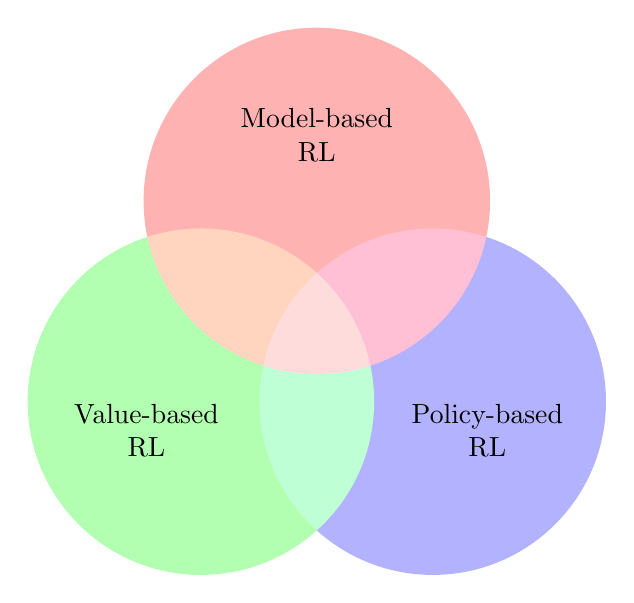
\begin{tikzpicture}
 \begin{scope}[blend group = soft light]
 \fill[red!30!white] ( 90:1.7) circle (2.2);
 \fill[green!30!white] (210:1.7) circle (2.2);
 \fill[blue!30!white] (330:1.7) circle (2.2);
 \end{scope}
 \node at ( 90:2.5) {
 \begin{tabular}{c}
 \text{Model-based}\\
 \text{RL} \\
 \end{tabular}
 };
 \node at ( 210:2.5) {
 \begin{tabular}{c}
 \text{Value-based}\\
 \text{RL} \\
 \end{tabular}
 };
 \node at ( 330:2.5) {
 \begin{tabular}{c}
 \text{Policy-based}\\
 \text{RL} \\
 \end{tabular}
 };
\end{tikzpicture}
}
\end{figure}
\end{frame}

\begin{frame}\frametitle{DQN}
	\[Q^\pi(s,a)=\mathbb{E}\left[\sum\limits_{t=0}^\infty\gamma^tr_t\,\middle|\, s,a\right]\]
	\[\max_\pi Q^\pi(s,a)\eqqcolon Q^*(s,a)=\mathbb{E}_{s'}\left[r+\gamma\max_{a'}Q^*(s',a')\,\middle|\, s,a\right]\]
	\[Q_{t+1}(s,a)=\mathbb{E}_{s'}\left[r+\gamma\max_{a'}Q_t(s',a')\,\middle|\, s,a\right]\]
	\[\textcolor{yellow}{Q_t\xrightarrow{t\to\infty}Q^*}\]
	\[Q_{t+1}(s,a)=Q_t(s,a)+\alpha\left(r+\gamma\max\limits_{a'} Q_t(s',a')-Q_t(s,a)\right)\]
	\[\textcolor{red}{Q(s,a;\theta)\approx Q^*(s,a)}\]
	\[L(\theta)\coloneqq \mathbb{E}_{s,a,r,s'}\left[\Big(r+\gamma\max\limits_{a'} Q\left(s',a';\theta^-\right)-Q(s,a;\theta)\Big)^2\right]\tag{DQN}\]
\end{frame}

\begin{frame}\frametitle{DQN}
	\[L(\theta)\coloneqq \mathbb{E}_{s,a,r,s'}\left[\Big(r+\gamma Q\big(s',\argmax\limits_{a'} Q(s',a';\theta);\theta^-\big)-Q(s,a;\theta)\Big)^2\right]\tag{Double DQN}\]
	
	\[Q(s,a)=V(s;\theta)+A(s,a;\theta')\tag{Dueling Network}\]
\end{frame}

\begin{frame}\frametitle{Actor-Critic Learning}
\begin{itemize}
	\item Combination of policy learning and $Q$ learning
	\begin{itemize}
		\item actor: move predictor (as in policy learning) $s\to a$
		\item critic: value of state (as in $Q$ learning) $V(s)$
	\end{itemize}
	\item We use this setup to influence how much to boost good moves
	\begin{itemize}
		\item advantage $A = R-V(s)$
		\item good moves when advantage is high
	\end{itemize}
\end{itemize}
	\[\left\{\begin{aligned}
	&\nabla_\theta\log\pi(a_t\mid s_t;\theta)\left(\sum\limits_{i=0}^{k-1}\gamma^ir_{t+i}+\gamma^k V(s_{t+k};\theta')-V(s_t;\theta')\right)&\text{actor}\\
	&\nabla_{\theta'}\left(\sum\limits_{i=0}^{k-1}\gamma^ir_{t+i}+\gamma^k V(s_{t+k};\theta')-V(s_t;\theta')\right)^2&\text{critic}
	\end{aligned}\right.\tag{AC}
	\]
\end{frame}

\begin{frame}\frametitle{Go}
\begin{figure}[H]
\subfigure{\includegraphics[height=.45\textwidth]{img/go1.pdf}}\;\;
\subfigure{\includegraphics[height=.45\textwidth]{img/go2.pdf}}
\end{figure}
\end{frame}

\begin{frame}\frametitle{AlphaZero}
\[{\footnotesize
\begin{tikzcd}
\text{$current\atop player$} \arrow[r] \& \boxed{\mbox{policy evaluation}\atop\mbox{\textcolor{yellow}{neural network}}} \arrow[rr, "\tiny\mbox{position `value'}\atop\mbox{move `probability'}"] \&\& \boxed{\mbox{policy improvement}\atop\mbox{\textcolor{yellow}{neural network}}} \arrow[r] \& \text{$improved\atop player$} \arrow[llll,bend left=20,"\mbox{self-learning/policy iteration}"]
\end{tikzcd}}\]
\begin{columns}
\column{.43\textwidth}
	\begin{figure}
	\includegraphics[width=\textwidth]{img/alphazero}
	\end{figure}
\column{.42\textwidth}
	\[(\mathbf{p},v)=f_\theta(s)\]
	\[l=(z-v)^2-\pi^\mathsf{T}\log\mathbf{p}+c\|\theta\|^2\]
	\[\pi_t\gets\operatorname{MCTS}(f_\theta(s_t))\]
	\[a_t\sim\pi_t\]
	\begin{block}{Intuition $+$ Calculation}\centering
		CNN $+$ MCTS
	\end{block}
\end{columns}
\end{frame}

\begin{frame}\frametitle{From AlphaZero to MuZero}
\begin{figure}[H]
\includegraphics[width=\textwidth]{img/muzero-alphazero.png}
\end{figure}
MuZero is discovering for itself how to build a model and understand it just from first principles.
\end{frame}

\begin{frame}\frametitle{}
\setlength\abovedisplayskip{0pt}
\setlength\belowdisplayskip{0pt}
\begin{figure}[H]
\includegraphics[width=\textwidth]{img/muzero.png}
\end{figure}
\begin{itemize}
	\item Model
\begin{align*}
&\left.
\begin{array}{rl}
s^0 &= h_\theta(o_1, \dots, o_t) \\
r^k, s^k &= g_\theta(s^{k-1}, a^k) \\
%
\mathbf{p}^k, v^k &= f_\theta(s^k)
\end{array}
\right\} \;\;
\mathbf{p}^k, v^k, r^k = \mu_\theta(o_1, \dots, o_t, a^1, \dots, a^k)
\end{align*}
	\item Search
\begin{align*}
\nu_t, \pi_t &= \operatorname{MCTS}(s^0_t, \mu_\theta) \\
a_t &\sim \pi_t \\
\end{align*}
\end{itemize}
\end{frame}

\begin{frame}\frametitle{MuZero}
\begin{itemize}
	\item \textbf{(A)} How MuZero uses its model to plan. The model consists of three connected components for representation $h$, dynamics $g$ and prediction $f$. The initial hidden state $s^0$ is obtained by passing the past observations $o_1,\dots,o_t$ into a \emph{representation} function $h$.
	\item \textbf{(B)} How MuZero acts in the environment. A MCTS is performed at each timestep $t$. An action $a_{t+1}$ is sampled from the search policy $\pi_t$, which is proportional to the visit count for each action from the root node. The environment receives the action and generates a new observation $o_{t+1}$ and reward $u_{t+1}$.
	\item \textbf{(C)} How MuZero trains its model. For the initial step, the representation function $h$ receives as input the past observations $o_1,\dots,o_t$. At each step $k$, the dynamics function $g$ receives as input the hidden state $s^{k-1}$ from the previous step and the real action $a_{t+k}$. The parameters of the representation, dynamics and prediction functions are jointly trained to predict three quantities: the policy $\mathbf{p}^k \approx \pi_{t+k}$, value function $v^k \approx z_{t+k}$, and reward $r_{t+k} \approx u_{t+k}$.
\end{itemize}
\end{frame}

\begin{frame}\frametitle{The MuZero loss function}
\[
l_t(\theta) = \sum_{k=0}^K l^r (u_{t+k}, r_t^k) + l^v(z_{t+k}, v^k_t) + l^p(\pi_{t+k}, \mathbf{p}^k_t) + c\|\theta\|^2
\]
\begin{enumerate}
	\item The difference between the predicted reward $k$ steps ahead of turn $t$ ($r$) and the actual reward ($u$).
	\item The difference between the predicted value $k$ steps ahead of turn $t$ ($v$) and the TD target value ($z$).
	\item The difference between the predicted policy $k$ steps ahead of turn $t$ ($p$) and the MCTS policy ($\pi$).
\end{enumerate}
\end{frame}

\begin{frame}\frametitle{GAN --- Generative Adversarial Network}
	\[V(D,G)=\mathbb{E}_{x\sim P_{data}}\left[\log{D(x)}\right]+\mathbb{E}_{z\sim P_{noise}}\left[\log{(1-D(G(z)))}\right]\]
	\[G^*=\argmin\limits_G\max\limits_DV(D,G)\tag{GAN}\]
	\begin{figure}[H]
	\includegraphics[width=.9\textwidth,angle=0,origin=c]{img/gan.png}
	\end{figure}
\end{frame}

\begin{frame}\frametitle{GAN}
\begin{figure}[H]
\includegraphics[width=\textwidth]{img/gan1.png}
\end{figure}
\end{frame}

\begin{frame}\frametitle{Minimal Sufficient Statistic}
\begin{definition}[Sufficient Statistic]
Let $Y$ be a parameter indexing a family of probability distributions. Let $X$ be random variable drawn from a probability distribution determined by $Y$. $T(X)$ is a sufficient statistic for $Y$ iff $X$ is independent of $Y$ given $T(X)$, i.e. $p(x\mid t,y)=p(x\mid t)$.
\end{definition}
\begin{definition}[Minimal Sufficient Statistic]
A sufficient statistic $S(X)$ is minimal iff for any sufficient statistic $T(X)$, there exists a function $f$ s.t. $S=f(T)$ almost everywhere w.r.t $X$.
\end{definition}
\begin{theorem}
\begin{itemize}
\item $T$ is sufficient statistics for $Y$ $\iff$ $I(T(X);Y)=I(X;Y)$.
\item $S$ is minimal sufficient statistics for $Y$ $\implies$ $I(X;S(X))\leq I(X;T(X))$.
\end{itemize}
\end{theorem}
\end{frame}

\begin{frame}\frametitle{\href{http://naftali-tishby.strikingly.com/}{Information Bottleneck --- Learning is to forget!}}
\begin{theorem}
Let $X$ be a sample drawn according to a distribution determined by the random variable $Y$. The set of solutions to
\[\min\limits_T I(X;T)\quad s.t.\quad I(T;Y)=\max\limits_{T^\prime}I(T^\prime;Y)\]
is exactly the set of minimal sufficient statistics for $Y$ based on $X$.
\end{theorem}
Find a random variable $T$ s.t.:
\begin{itemize}
	\item $Y\leftrightarrow X\leftrightarrow T$ form a Markov chain.
	\item $I(X;T)$ is minimized (minimality, \textcolor{yellow}{complexity} term), while\\ $I(T;Y)$ is maximized (sufficiency, \textcolor{yellow}{accuracy} term).
\end{itemize}
\[\fbox{$T^*\coloneqq \argmin\limits_{T: I(T(X);Y)=I(X;Y)}I(X;T(X))$}\] is the \textcolor{yellow}{Information Bottleneck} between $X$ and $Y$.
\end{frame}

\begin{frame}\frametitle{}\vspace{-1ex}
\begin{columns}
\column{.51\textwidth}
\begin{figure}[H]
\includegraphics[width=\textwidth,angle=0,origin=c]{img/encoder-decoder}
\includegraphics[width=\textwidth,angle=0,origin=c]{img/bottleneck}
\end{figure}
\column{.4\textwidth}
张三丰:将所见到的剑招忘得半点不剩,才能得其神髓。\\
\vspace*{2ex}
老子:为学日益,为道日损。\\损之又损,以至于无为。\\无为而无不为。
\end{columns}
\end{frame}

\begin{frame}\frametitle{Information Bottleneck}
$\min\limits_{p(t\mid x),p(t),p(y\mid t)}\Big\{I(X;T)-\beta I(T;Y)\Big\}$ subject to Markov chain $Y\to X\to T$.
\[L[p(t\mid x)]\coloneqq I(X;T)-\beta I(T;Y)-\sum\limits_x\lambda(x)\sum\limits_t p(t\mid x)\]
Let
\[\frac{\delta L}{\delta p(t\mid x)}=0\]
The solution is
\begin{align*}
p(t\mid x)&=\frac{p(t)}{Z(x,\beta)}\mathrm{e}^{-\beta D[p(y\mid x)\|p(y\mid t)]}\\
p(t)&=\sum\limits_x p(t\mid x)p(x)\\
p(y\mid t)&=\frac{1}{p(t)}\sum\limits_x p(t\mid x)p(x,y)
\end{align*}
\end{frame}

\begin{frame}\frametitle{The Information Bottleneck Method\footnote{\tiny Schwartz-Ziv, Tishby: Opening the black box of Deep Neural Networks via Information.}}
\begin{algorithm}[H]
\begin{algorithmic}[1]
\State Given $p(x,y)$, $\beta \geq 0$
\State Initialize $p^{(0)}(t\mid x)$
\State $p^{(0)}(t)=\sum_x p^{(0)}(t\mid x)p(x)$
\State $p^{(0)}(y\mid t)=\frac{1}{p^{(0)}(t)}\sum_x p^{(0)}(t\mid x)p(x,y)$
\State $n=0$
\While{not converged}
\State $n=n+1$
\State $p^{(n)}(t\mid x)=\frac{p^{(n-1)}(t)}{Z(x,\beta)}\mathrm{e}^{-\beta D\left[p(y\mid x)\| p^{(n-1)}(y\mid t)\right]}$
\State $p^{(n)}(t)=\sum_x p^{(n)}(t\mid x)p(x)$
\State $p^{(n)}(y\mid t)=\frac{1}{p^{(n)}(t)}\sum_x p^{(n)}(t\mid x)p(x,y)$
\EndWhile
\end{algorithmic}\caption{The Information Bottleneck Method}
\end{algorithm}
\end{frame}

\begin{frame}\frametitle{The Deterministic Information Bottleneck}
\[L_\alpha[p(t\mid x)]\coloneqq H(T)-\alpha H(T\mid X)-\beta I(T;Y)-\sum\limits_x\lambda(x)\sum\limits_t p(t\mid x)\]
\[p(t\mid x)=\frac{1}{Z(x,\alpha,\beta)}\mathrm{e}^{\frac{1}{\alpha}\big(\log p(t)-\beta D[p(y\mid x)\|p(y\mid t)]\big)}\]
Obviously, $L_1=L$.
\begin{align*}
p_\alpha(t\mid x)&=\frac{1}{Z(x,\alpha,\beta)}\mathrm{e}^{\frac{1}{\alpha}\left(\log p_\alpha(t)-\beta D[p(y\mid x)\|p_\alpha(y\mid t)]\right)}\\
p_\alpha(t)&=\sum\limits_x p_\alpha(t\mid x)p(x)\\
p_\alpha(y\mid t)&=\frac{1}{p_\alpha(t)}\sum\limits_x p_\alpha(t\mid x)p(x,y)
\end{align*}
Let $\alpha\to 0$, we get the deterministic case
\[p(t\mid x)=\lim\limits_{\alpha\to 0}p_\alpha(t\mid x)=\left\llbracket t=\argmax\limits_t\Big(\log p(t)-\beta D[p(y\mid x)\|p(y\mid t)]\Big)\right\rrbracket\]
\end{frame}

\begin{frame}\frametitle{The Deterministic Information Bottleneck Method}
\begin{algorithm}[H]
\begin{algorithmic}[1]
\State Given $p(x,y)$, $\beta \geq 0$
\State Initialize $f^{(0)}(x)$
\State $p^{(0)}(t)=\sum_{x:f^{(0)}(x)=t} p(x)$
\State $p^{(0)}(y\mid t)=\frac{\sum_{x:f^{(0)}(x)=t} p(x,y)}{\sum_{x:f^{(0)}(x)=t} p(x)}$
\State $n=0$
\While{not converged}
\State $n=n+1$
\State $f^{(n)}(x)=\argmax\limits_t\Big(\log p^{(n-1)}(t)-\beta D\left[p(y\mid x)\| p^{(n-1)}(y\mid t)\right]\Big)$
\State $p^{(n)}(t)=\sum_{x:f^{(n)}(x)=t} p(x)$
\State $p^{(n)}(y\mid t)=\frac{\sum_{x:f^{(n)}(x)=t} p(x,y)}{\sum_{x:f^{(n)}(x)=t} p(x)}$
\EndWhile
\end{algorithmic}\caption{The Deterministic Information Bottleneck Method}
\end{algorithm}
\end{frame}

\begin{frame}\frametitle{Expressiveness \& Sample Complexity}
Smooth functions require fewer neurons to approximate.
	\begin{theorem}
		The hypothesis class of neural networks of depth $T$ and size $O(T^2)$ contains all functions that can be implemented by a Turing machine within $T$ operations, while having $O(T^2)$ sample complexity.
	\end{theorem}
\end{frame}

\begin{frame}\frametitle{The Ultimate Hypothesis Space}
\begin{itemize}
	\item \textcolor{yellow}{No Free Lunch:} Sample complexity is exponentially large (w.r.t. the input dimension) if the hypothesis class is all possible functions.
	\item \textcolor{yellow}{Shallow learning (SVM, Boosting):} Hypothesis class is linear functions over manually determined features --- strong prior knowledge.
	\item \textcolor{yellow}{Deep learning:} Hypothesis class is all functions implemented by determining the weights of a given artificial neural network.
\end{itemize}\vspace{-1ex}
	\begin{figure}[H]
	\includegraphics[width=.7\textwidth,angle=0,origin=c]{img/priornfl}\vspace{-2ex}\caption{Prior vs Universality}
	\end{figure}
	\[\fbox{\textbf{\textcolor{red}{Prior --- a necessary good or a necessary evil?}}}\]
\end{frame}


%%%%%%%%%%%%%%%%%%%%%%%%%%%%%%%%
\section{Artificial General Intelligence}
%%%%%%%%%%%%%%%%%%%%%%%%%%%%%%%%


%--------------------------%
\subsection{AIXI}
%--------------------------%

\begin{frame}\frametitle{UAI}
	\begin{enumerate}
		\item Solve intelligence
		\item Use it to solve everything else
	\end{enumerate}
	\begin{itemize}
		\item learn automatically from raw inputs --- not pre-programmed.
		\item same algorithm, different tasks.
	\end{itemize}
\end{frame}

\begin{frame}\frametitle{UAI}
	\begin{columns}
		\column{.6\textwidth}\vspace{-4ex}
			\begin{table}
\abovetabulinesep=1mm
\belowtabulinesep=1mm
				\begin{tabu}{c|c}
					\hline
					\large \textcolor{red}{(Deep) RL} &\large\textcolor{red}{General RL}\\
					\hline
					state space &history\\
					\hline
					ergodic &not ergodic\\
					\hline
					fully observable &partially observable\\
					\hline
					$\varepsilon$-exploration works &$\varepsilon$-exploration fails\\
					\hline
					\Large\textcolor{yellow}{MDP/DQN} &\Large\textcolor{yellow}{AIXI}\\
					\hline
				\end{tabu}\caption{(Deep) RL vs General RL}
			\end{table}
		\column{.4\textwidth}\hspace{-0.4\textwidth}
			\resizebox{.8\textwidth}{!}{	\begin{minipage}{\textwidth}
					\begin{center}
						\unitlength=2ex
						\linethickness{0.4pt}
						\begin{picture}(32,20)(0,0)
						\thicklines
						% boxes
						\put(16,17.5){\oval(5,3)\makebox(0,0)[cc]{UAI}}
						\put(16,12){\oval(7,2)\makebox(0,0)[cc]{Framework}}
						\put(11,6){\oval(5,2)\makebox(0,0)[cc]{\textcolor{green}{Learning}}}
						\put(16,6){\oval(4,2)\makebox(0,0)[cc]{Utility}}
						\put(21,6){\oval(5,2)\makebox(0,0)[cc]{\textcolor{green}{Planning}}}
						\thinlines
						\put(16,13){\line(0,4){3}}
						\put(11,7){\line(3,4){3}}
						\put(16,7){\line(0,4){4}}
						\put(21,7){\line(-3,4){3}}
						\end{picture}
					\end{center}
			\end{minipage}}
	\end{columns}\vspace{-5ex}
	\begin{center}
		\boxed{
			\begin{minipage}{60ex}\centering
				\begin{large}
					\begin{tabu}{ccc}
						\textcolor{green}{Decision Theory} & $=$ & \textcolor{green}{Probability $+$ Utility Theory} \\
						$+$ & & $+$ \\
						\textcolor{red}{Universal Induction} & $=$ & \textcolor{red}{Occam $+$ Bayes $+$ Turing} \\
						$\scriptstyle||$ & & $\scriptstyle||$ \\
						\multicolumn{3}{c}{\textcolor{yellow}{Universal Artificial Intelligence without Parameters}} \\
					\end{tabu}
				\end{large}
		\end{minipage}}
	\end{center}
\end{frame}

\begin{frame}\frametitle{Induction $\implies$ Prediction $\implies$ Decision $\implies$ Action}
\begin{figure}[H]
\includegraphics[width=.18\textwidth]{img/learning-baby.jpg} $\implies$
\includegraphics[width=.18\textwidth]{img/predict-scientist.jpg} $\implies$
\includegraphics[width=.18\textwidth]{img/planning-engineer.jpg} $\implies$
\includegraphics[width=.18\textwidth]{img/action-go.jpg}
\end{figure}
\begin{example}
\begin{itemize}
	\item Induction: Find a model of the world economy.
	\item Prediction: Use the model for predicting the future stock market.
	\item Decision: Decide whether to invest assets in stocks or bonds.
	\item Action: Trading large quantities of stocks influences the market.
\end{itemize}	
\end{example}
\end{frame}

\begin{frame}\frametitle{Marcus Hutter}
			\begin{figure}
				\subfigure{\includegraphics[height=.4\textwidth,angle=0,origin=c]{img/uai.jpeg}}
				\subfigure{\includegraphics[height=.4\textwidth,angle=0,origin=c]{img/hutter.jpg}}
			\end{figure}
	Jan Leike, Tor Lattimore, Shane Legg, Joel Veness, Laurent Orseau, Mark Ring, Peter Sunehag, Mayank Daswani, Tom Everitt, Jan Poland, Daniel Filan, William Uther, Kee Siong Ng, David Silver, J\"urgen Schmidhuber, Alexey Potapov, Bill Hibbard, Daniil Ryabko, Alexey Chernov, Michael Cohen\dots
\end{frame}

\begin{frame}\frametitle{}
\[
{\footnotesize
\begin{tikzcd}
\boxed{\large sensors} \arrow[d]\\
\boxed{\text{What the world}\atop \text{is like now}} \arrow[d]\\
\boxed{\text{What it will be like}\atop \text{if I do action $a$}} \arrow[d] \& \text{\textit{\textbf{\underline{\huge{\textcolor{red}{Agent}}}}}} \& \boxed{\boxed{\text{\textit{\textbf{\underline{\Large\textcolor{yellow}{{Environment}}}}}}}} \arrow[uull,Rightarrow,"perception",marking]\\
\boxed{\text{How happy I will be}\atop \text{in such a state}} \arrow[d]\\
\boxed{\text{What action}\atop \text{I should do now}} \arrow[d]\\
\boxed{\large Effectors} \arrow[uuurr,Rightarrow,"action" swap,marking]
\end{tikzcd}
}
\]
\end{frame}

\begin{frame}\frametitle{Computationalism}
	\begin{figure}[H]
				\hspace{-17pt}
					\begin{center}
						\unitlength=1.1mm
						\large
						\begin{picture}(106,47)
						\thicklines
						\put(1,41){\framebox(16,6)[cc]{\textcolor{yellow}{$e_1$}}}
						\put(17,41){\framebox(16,6)[cc]{\textcolor{yellow}{$e_2$}}}
						\put(33,41){\framebox(16,6)[cc]{\textcolor{yellow}{$e_3$}}}
						\put(49,41){\framebox(16,6)[cc]{\textcolor{yellow}{$e_4$}}}
						\put(65,41){\framebox(16,6)[cc]{\textcolor{yellow}{$e_5$}}}
						\put(81,41){\framebox(16,6)[cc]{\textcolor{yellow}{$e_6$}}}
						\put(97,47){\line(1,0){9}}\put(97,41){\line(1,0){9}}\put(102,44){\makebox(0,0)[cc]{\ldots}}
						\put(1,1){\framebox(16,6)[cc]{\textcolor{red}{$a_1$}}}
						\put(17,1){\framebox(16,6)[cc]{\textcolor{red}{$a_2$}}}
						\put(33,1){\framebox(16,6)[cc]{\textcolor{red}{$a_3$}}}
						\put(49,1){\framebox(16,6)[cc]{\textcolor{red}{$a_4$}}}
						\put(65,1){\framebox(16,6)[cc]{\textcolor{red}{$a_5$}}}
						\put(81,1){\framebox(16,6)[cc]{\textcolor{red}{$a_6$}}}
						\put(97,7){\line(1,0){9}}\put(97,1){\line(1,0){9}}\put(102,4){\makebox(0,0)[cc]{\ldots}}
						%
						\textcolor{red}{\put(1,21){\framebox(16,6)[cc]{\text{work}}}}
						\thicklines
						\put(17,17){\textcolor{red}{\framebox(20,14)[cc]{$\displaystyle{\begin{array}{c}
										\textcolor{red}{\textbf{Agent}}\atop
										\textcolor{red}{\mathbf{\pi}}
										\end{array}}$}}}
						%\thinlines
						\textcolor{red}{\put(37,27){\line(1,0){14}}}
						\textcolor{red}{\put(36,21){\line(1,0){14}}}
						\textcolor{red}{\put(39,24){\makebox(0,0)[lc]{\text{tape}\ldots}}}
						%
						\textcolor{yellow}{\put(56,21){\framebox(16,6)[cc]{\text{work}}}}
						\thicklines
						\put(72,17){\textcolor{yellow}{\framebox(20,14)[cc]{$\displaystyle{\begin{array}{l}
										\textcolor{yellow}{\textbf{Environment}}\atop
										\textcolor{yellow}{\mathbf{\mu}}
										\end{array}}$}}}
						%\thinlines
						\textcolor{yellow}{\put(92,27){\line(1,0){14}}}
						\textcolor{yellow}{\put(91,21){\line(1,0){14}}}
						\textcolor{yellow}{\put(94,24){\makebox(0,0)[lc]{\text{tape}\ldots}}}
						%
						\normalcolor
						\thicklines
						\textcolor{red}{\put(46,41){\vector(-2,-1){20}}}
						\textcolor{yellow}{\put(81,31){\vector(-2,1){20}}}
						\textcolor{yellow}{\put(47,7){\vector(3,1){30}}}
						\textcolor{red}{\put(17,17){\vector(3,-1){30}}}
						\end{picture}
					\end{center}
	\end{figure}
\end{frame}

\begin{frame}\frametitle{Agent \& Environment}
\begin{definition}[Agent \& Environment]
	\begin{columns}
		\column{.75\textwidth}
				\begin{itemize}
					\item finite set of possible actions $\mathcal{A}$ and perceptions $\mathcal{E}$;
					\item prior knowledge $w\in\Delta\mathcal{M}$ of the environments $\mathcal{M}$;
					\item utility function $u:({\mathcal{A}} \times {\mathcal{E}})^*\to[0,1]$;
					\item discount factor $\gamma\in[0,1]$;
				\end{itemize}
				\[\pi:(\mathcal{A}\times\mathcal{E})^*\to\Delta\mathcal{A}\]
				\[\mu: (\mathcal{A}\times\mathcal{E})^*\times\mathcal{A}\to\Delta\mathcal{E}\]
				\[P_\mu^\pi(\ae_{<t})\coloneqq \prod\limits_{i=1}^{t-1}\pi(a_i\mid \ae_{<i})\mu(e_i\mid \ae_{<i}a_i)\]
		\column{.25\textwidth}\hspace{-11ex}
			\resizebox{\textwidth}{!}{
				\begin{minipage}{\textwidth}
					\begin{figure}[H]
						\tikzstyle{mcirc}=[draw, circle, fill=none]
						\tikzstyle{line}=[draw, -latex',font=\scriptsize]
						\begin{tikzpicture}
						\node [mcirc] (s0) at (0,0) {$\text{agent} \atop \pi$};
						\node [mcirc] (s1) at (3,0) {$\text{environment} \atop \mu$};
						\path [line] (s0) edge [bend right=50] node [midway, below] {action} (s1);
						\path [line] (s0) edge [bend right=50] node [midway, above] {$a$} (s1);
						\path [line] (s1) edge [bend right=50] node [midway, above] {perception} (s0);
						\path [line] (s1) edge [bend right=50] node [midway, below] {$e$} (s0);
						\end{tikzpicture}
					\end{figure}
			\end{minipage}}
	\end{columns}
\end{definition}
\end{frame}

\begin{frame}\frametitle{Value Function}
	\[r_n\coloneqq u(\ae_{1:n})\]
	\[V_\mu^\pi(\ae_{<t})\coloneqq \mathbb{E}_\mu^\pi\left[\sum\limits_{k=0}^\infty\gamma^k r_{t+k}\,\middle|\, \ae_{<t}\right]\]
	\textcolor{yellow}{Bellman equation:}
	\begin{align*}
	V_\mu^\pi(\ae_{<k})&=\sum\limits_{a_k\in\mathcal{A}}\pi(a_k\mid \ae_{<k})\sum\limits_{e_k\in\mathcal{E}}\mu(e_k\mid \ae_{<k}a_k)\left[r_k+\gamma V_\mu^\pi(\ae_{1:k})\right]\tag{\text{\tiny{recursive}}}\\
	&\textcolor{red}{=}\sum\limits_{\ae_{k:m}}P_\mu^\pi(\ae_{k:m}\mid \ae_{<k})\left[\sum\limits_{i=k}^m \gamma^{i-k} r_i+\gamma^{m-k+1} V_\mu^\pi(\ae_{1:m})\right]\tag{\text{\tiny{iterative}}}
	\end{align*}
	\[V_\mu^\pi(\ae_{<k})=\lim\limits_{m\to\infty}\sum\limits_{\ae_{k:m}}P_\mu^\pi(\ae_{k:m}\mid \ae_{<k})\left[\sum\limits_{i=k}^m\gamma^{i-k}r_i\right]\]
\end{frame}

\begin{frame}\frametitle{Optimal Value/Policy}
	\[V_\mu^*\coloneqq \max\limits_\pi V_\mu^\pi\]
	\begin{align*}
	V_\mu^*(\ae_{<k})&=\lim\limits_{m\to\infty}\max\limits_{a_k\in\mathcal{A}}\sum\limits_{e_k\in\mathcal{E}}\cdots \max\limits_{a_m\in\mathcal{A}}\sum\limits_{e_m\in\mathcal{E}}\sum\limits_{i=k}^m\gamma^{i-k}r_i\prod\limits_{j=k}^i \mu(e_j\mid \ae_{<j}a_j)\\
	&\textcolor{red}{=}\lim\limits_{m\to\infty}\max\limits_{a_k\in\mathcal{A}}\sum\limits_{e_k\in\mathcal{E}}\cdots \max\limits_{a_m\in\mathcal{A}}\sum\limits_{e_m\in\mathcal{E}}\left[\sum\limits_{i=k}^m\gamma^{i-k}r_i\right]\mu(e_{k:m}\mid \ae_{<k}a_{k:m})
	\end{align*}
	
	\[\pi_\mu^*\coloneqq \argmax\limits_\pi V_\mu^\pi\]
\end{frame}

\begin{frame}\frametitle{Bayesian Mixture \& Belief Update}
	\[\xi(e_{<n}\mid a_{<n})\coloneqq \sum\limits_{\nu \in \mathcal{M}} w_\nu \nu(e_{<n}\mid a_{<n})\]
	\[w_{\ae_{<n}}^\nu\coloneqq \dfrac{w_\nu \nu(e_{<n} \mid a_{<n})}{\xi(e_{<n}\mid a_{<n})}\]
	\[\resizebox{\textwidth}{!}{$\sum\limits_{k=1}^\infty \sum\limits_{e_{1:k}} \mu(e_{<k} \mid a_{<k}) \Big(\mu(e_k\mid \ae_{<k}a_k) - \xi(e_k\mid \ae_{<k}a_k ) \Big)^2\leq\min\limits_{\nu\in\mathcal{M}}\Big\{-\ln w_\nu+D(\mu\|\nu)\Big\}$}
	\]
\begin{center}
What probability should an observer assign to future experiences if she is told that she will be simulated on a computer?
\end{center}
\end{frame}

\begin{frame}\frametitle{Intelligence Measure \& AIXI}
\setlength\abovedisplayskip{0pt}
\setlength\belowdisplayskip{0pt}
	\begin{center}
		\huge What is `\textcolor{red}{intelligence}'?
	\end{center}
	\begin{center}
		A Blind Man in a Dark Room Looking for a Black Cat That Is Not There?
	\end{center}
	\begin{quote}
		Intelligence measures an agent's ability to achieve goals in a wide range of environments.\par
		\hfill --- \textsl{Shane Legg and Marcus Hutter}
	\end{quote}
	\begin{center}
		\boxed{
			\begin{minipage}{60ex}
				\begin{align*}
				\Upsilon(\pi)&\coloneqq \sum\limits_{\nu\in\mathcal{M}}w_\nu V_\nu^\pi(\epsilon)=V_\xi^\pi(\epsilon)\tag{\textcolor{red}{Intelligence Measure}}\\
				\textcolor{yellow}{\mathrm{AIXI}}&\coloneqq \argmax\limits_\pi\Upsilon(\pi)=\pi_\xi^*
				\end{align*}
		\end{minipage}}
	\end{center}
	\[V_\xi^\pi(h)=\sum\limits_{\nu\in\mathcal{M}}w_h^\nu V_\nu^\pi(h)\]
	\[\textcolor{yellow}{w_\nu\coloneqq 2^{-K(\nu)}}\implies\xi(e_{1:m}\mid a_{1:m})\eqm M(e_{1:m}\mid a_{1:m})\coloneqq \textcolor{yellow}{\sum\limits_{p:U(p,a_{1:m})=e_{1:m}}\!\!2^{-\ell(p)}}\]
\end{frame}

\begin{frame}\frametitle{AIXI}\vspace{-3ex}
\[a_k^*\;\coloneqq \;\argmax_{a_k}\sum_{e_k}\dots \max_{a_m}\sum_{e_m}\left[\sum\limits_{i=k}^m \gamma^{i-k}r_i\right]\!\sum\limits_{p:U(p,{a_{1:m}})=e_{1:m}}\!\!\!\!\!\!\!\!\!\!\! 2^{-\ell(p)}\tag{AIXI}\]
	\begin{figure}[!htb]\vspace{-1ex}
		\begin{center}
			\resizebox{\textwidth}{!}{
				\boxed{
					\begin{minipage}{75ex}
						\begin{center}
							\small
							\unitlength=1mm\vspace{-4ex}
							\begin{picture}(145,60)(10,10)
							\thicklines
							\textcolor{red}{
								\put(50,60){\circle*{1.5}}
								\put(50,60){\line(-1,-1){20}}
								\put(39,47){\makebox(0,0)[lc]{$a_k\!=0$}}
								\put(50,60){\line(1,-1){20}}
								\put(61,47){\makebox(0,0)[rc]{$a_k\!=1$}}
								\put(50,55){\makebox(0,0)[ct]{$\underbrace{\;\textcolor{orange}{max}\;}$}}
								\put(55,59){\makebox(0,0)[lc]{$\scriptstyle V_\mu^*(\ae_{<k})=\max\limits_{a_k} Q_\mu^*(\ae_{<k}a_k)$}}
								% observation $e_k$
							}\textcolor{yellow}{
								\put(30,40){\circle*{1}}
								\put(30,40){\line(-1,-2){10}}
								\put(27,27){\makebox(0,0)[lc]{$\scriptstyle e_k=?$}}
								\put(22,23){\makebox(0,0)[lc]{$\scriptstyle u(\ae_{1:k})=?$}}
								\put(30,40){\line(1,-2){10}}
								\put(30,35){\makebox(0,0)[ct]{$\underbrace{\textcolor{orange}{\mathbb{E}}}$}}
								\put(70,40){\circle*{1}}
								\put(70,40){\line(-1,-2){10}}
								\put(70,40){\line(1,-2){10}}
								\put(73,27){\makebox(0,0)[rc]{$\scriptstyle e_k=?$}}
								\put(77.5,23){\makebox(0,0)[rc]{$\scriptstyle u(\ae_{1:k})=?$}}
								\put(70,35){\makebox(0,0)[ct]{$\underbrace{\textcolor{orange}{\mathbb{E}}}$}}
								\put(75,39){\makebox(0,0)[lc]{$\scriptstyle Q_\mu^*(\ae_{<k}a_k)=\sum\limits_{e_k}\mu(e_k\mid\ae_{<k}a_k)\left[r_k+\gamma V_\mu^*(\ae_{1:k})\right]$}}
								% action $a_{k+1}$
								\normalcolor}\textcolor{green}{
								\thinlines
								\put(20,20){\circle*{0.8}}
								\put(20,20){\line(-1,-2){5}}
								\put(20,20){\line(1,-2){5}}
								\put(20,14){\makebox(0,0)[ct]{${{\scriptscriptstyle \textcolor{orange}{max}}\atop \smile}$}}
								\put(30,15){\makebox(0,0)[cc]{$\scriptstyle a_{k+1}$}}
								\put(40,20){\circle*{0.8}}
								\put(40,20){\line(-1,-2){5}}
								\put(40,20){\line(1,-2){5}}
								\put(40,14){\makebox(0,0)[ct]{${{\scriptscriptstyle \textcolor{orange}{max}}\atop \smile}$}}
								\put(50,15){\makebox(0,0)[cc]{$\scriptstyle a_{k+1}$}}
								\put(60,20){\circle*{0.8}}
								\put(60,20){\line(-1,-2){5}}
								\put(60,20){\line(1,-2){5}}
								\put(60,14){\makebox(0,0)[ct]{${{\scriptscriptstyle \textcolor{orange}{max}}\atop \smile}$}}
								\put(70,15){\makebox(0,0)[cc]{$\scriptstyle a_{k+1}$}}
								\put(80,20){\circle*{0.8}}
								\put(80,20){\line(-1,-2){5}}
								\put(80,20){\line(1,-2){5}}
								\put(80,14){\makebox(0,0)[ct]{${{\scriptscriptstyle \textcolor{orange}{max}}\atop \smile}$}}
								\put(85,19){\makebox(0,0)[lc]{\scriptsize $\displaystyle V_\mu^*(\ae_{1:k})=\max\limits_{a_{k+1}}Q_\mu^*(\ae_{1:k}a_{k+1})$}}
								\put(15,8){\makebox(0,0)[cc]{$\vdots$}}
								\put(25,8){\makebox(0,0)[cc]{$\vdots$}}
								\put(35,8){\makebox(0,0)[cc]{$\vdots$}}
								\put(45,8){\makebox(0,0)[cc]{$\vdots$}}
								\put(55,8){\makebox(0,0)[cc]{$\vdots$}}
								\put(65,8){\makebox(0,0)[cc]{$\vdots$}}
								\put(75,8){\makebox(0,0)[cc]{$\vdots$}}
								\put(85,8){\makebox(0,0)[cc]{$\vdots$}}}
							\end{picture}\vspace{1ex}\caption{ExpectiMax}
						\end{center}
			\end{minipage}}}
		\end{center}
	\end{figure}
\end{frame}

\begin{frame}\frametitle{AIXI}
	\begin{figure}[H]
		\begin{center}
			\includegraphics[width=\textwidth,angle=0,origin=c]{img/aixi-environment}
		\end{center}
	\end{figure}
\end{frame}

\begin{frame}\frametitle{RL vs GRL}
	\begin{itemize}
		\item If $\mu$ is a completely observable MDP, $V_\mu^\pi$ reduces to the recursive Bellman equation.
		\item In a finite MDP, with a geometric discounting function, we can plan ahead by value iteration.
		\item According to Banach's fixpoint theorem, value iteration converges to the value of the optimal policy.
		\item What about GRL?
	\end{itemize}
\end{frame}

\begin{frame}\frametitle{}\vspace{-2ex}
\setlength\abovedisplayskip{0pt}
\setlength\belowdisplayskip{0pt}
	\[\text{discount } \gamma:\mathbb{N}^2\to[0,1]\;\;\text{and utility } u:(\mathcal{A}\times\mathcal{E})^*\to[0,1]\]
	\[V_t^{\pi\mu}(h_{<k})\coloneqq \mathbb{E}_\mu^\pi\left[\sum\limits_{i=k}^\infty \gamma_t^i u(h_{1:i})\,\middle|\, h_{<k}\right]\]
	\begin{block}{Assumption}
		\[
		\forall t\in\mathbb{N}^+: \lim\limits_{m\to\infty}\sup\limits_\pi\sum\limits_{h_{<m}}
		V_t^{\pi\mu}(h_{<m})P_\mu^\pi(h_{<m})=0
		\]
	\end{block}
	\begin{theorem}[Extreme Value Theorem]
		If $K$ is compact and $f: K\to\mathbb{R}$ is continuous, then $f$ is bounded and there exist $p,q\in K$ s.t. $f(p)=\sup_{x\in K}f(x)$ and $f(q)=\inf_{x\in K}f(x)$.
	\end{theorem}\vspace{-2ex}
	\[\left\langle\Pi\coloneqq \mathcal{A}^{(\mathcal{A}\times\mathcal{E})^*}, D(\pi,\pi')\coloneqq \mathrm{e}^{-\min\left\{n:\exists h_{<n}\left(\pi(h_{<n})\neq\pi'(h_{<n})\right)\right\}}\right\rangle\]\vspace{-2ex}
	\begin{center}
		\fbox{\textcolor{yellow}{$V_\mu^\pi(h):\Pi\to\mathbb{R}$ is continuous on the compact metric space $\left\langle\Pi,D\right\rangle$.}}
	\end{center}
	\[\pi_t^\mu\coloneqq \argmax\limits_\pi V_t^{\pi\mu}\qquad \pi^\mu(h_{<t})\coloneqq \pi_t^\mu(h_{<t})\]
\end{frame}

\begin{frame}\frametitle{Deterministic vs Stochastic}
	If \[\mu(e_{<t}\mid a_{<t})=\sum\limits_{p:U(p,a_{<t})=e_{<t}}\mu(p)\]
	then $\mu$ can be interpreted in \emph{two ways}:
	\begin{itemize}
		\item either the true environment is \textbf{deterministic}, but we only have \textbf{subjective belief} of which environment being the true environment; or
		\item the environment itself behaves \textbf{stochastically} defined by $\mu$.
	\end{itemize}
\end{frame}

\begin{frame}\frametitle{Intelligence vs Game}
\begin{minipage}{70ex}
\begin{table}[H]
\abovetabulinesep=1mm
\belowtabulinesep=1mm
\begin{tabu}{c|c|c}
					\hline
						&Game in $\mathcal{M}_D$ &Game in $\mathcal{M}_U$\\
						\hline
						Ex-post Equilibrium &Deterministic &\textcolor{red}{$\pi_\mu^*$}(recursive/iterative)\\
						\hline
						Bayesian-Nash Equilibrium & \textcolor{red}{$\pi_\mu^*$}(\textcolor{yellow}{functional}) &\textcolor{green}{$\pi_\xi^*$}(\textcolor{yellow}{functional})\\
					\hline
\end{tabu}
\end{table}
\end{minipage}
	\begin{center}
		\begin{minipage}{.87\textwidth}
			\begin{itemize}
				\item Ex-post expected utility $V_t^{\pi\mu}$\hfill \textcolor{red}{$V_\mu^\pi$}
				\item Ex-interim expected utility (\textcolor{yellow}{Intelligence Measure}) $V_t^{\pi\xi}$\hfill \textcolor{red}{$V_\xi^\pi$}
				\item Ex-post equilibrium $\pi_t^\mu$\hfill \textcolor{red}{$\pi_\mu^*$}
				\item Bayesian-Nash equilibrium $\pi_t^\xi$\hfill \textcolor{red}{$\pi_\xi^*$}
				\item Perfect Bayesian-Nash equilibrium $\pi^\xi$
			\end{itemize}
		\end{minipage}
	\end{center}
	\begin{center}
		\textcolor{green}{\Large Intelligence is an Equilibrium,\\
			We just have to Identify the Game.}
	\end{center}
	\[\text{Intelligence}=\underbrace{\text{Induction}+\text{Action}}_{\textit{efficiently}}\]
\end{frame}

\begin{frame}\frametitle{On-Policy Value Convergence for Bayes}
\begin{theorem}[On-Policy Value Convergence for Bayes]
For any environment $\mu\in\mathcal{M}$ and any policy $\pi$,
\[
P_\mu^\pi\left(\lim\limits_{t\to\infty}\left[V_\xi^\pi(\ae_{<t}) - V_\mu^\pi(\ae_{<t})\right]=0\right)=1
\]
\end{theorem}
\begin{itemize}
	\item Bayesian agents perform well at learning and achieve on-policy value convergence: the posterior belief about the value of a policy $\pi$ converges to the true value of $\pi$ while following $\pi$: $V^\pi_\xi(\ae_{<t})-V^\pi_\mu(\ae_{<t})\xrightarrow{t\to\infty}0$ $P_\mu^\pi$-almost surely.
	\item Since this holds for any policy, in particular it holds for the Bayes optimal policy $\pi^*_\xi$. This means that the Bayes agent learns to predict those parts of the environment that it sees. But if it does not explore enough, then it will not learn other parts of the environment that are potentially more rewarding.
\end{itemize}
\end{frame}

\begin{frame}\frametitle{AIXI}
	\begin{itemize}
		\item Intelligence measure: valid, informative, wide range, general, dynamic, unbiased, fundamental, formal, objective, fully defined, universal\textcolor{red}{?}
		\item AIXI is the most intelligent environmental independent, i.e. universally optimal, agent possible\textcolor{red}{?}
		\item Applications: Sequence Prediction, Games, Optimization, Supervised Learning, Classification\dots
		\item \textcolor{red}{AIXI is not limit computable, thus can't be approximated using finite computation. However there are limit computable $\varepsilon$-optimal approximations to AIXI.}
		\item \textcolor{red}{There are no known nontrivial and non-subjective optimality results for AIXI. General reinforcement learning is difficult even when disregarding computational costs.}
	\end{itemize}
\textbf{Remark:} Since AIXI is incomputable, it assigns zero probability to its own existence.
\end{frame}

\begin{frame}\frametitle{AIXI Depends on UTM/Prior! --- Dogmatic Prior}
\setlength\abovedisplayskip{0pt}
\setlength\belowdisplayskip{0pt}
	\begin{center}
	\includegraphics[clip=true,trim=30 10 10 40,width=.5\textwidth]{img/dogmatic-prior}
	\end{center}
	Dogmatic prior: if not acting according to one particular dogma $\pi$, got to hell with high probability. As long as the policy $\pi$ yields some rewards, the prior says that exploration would be too costly and AIXI does not dare to explore.
\end{frame}

\begin{frame}\frametitle{Dogmatic Prior}
\setlength\abovedisplayskip{0pt}
\setlength\belowdisplayskip{0pt}
	\begin{theorem}[Dogmatic Prior]
		Let $\pi$ be any computable deterministic policy, let $\xi$ be any Bayesian mixture over $\mathcal{M}_{\mathrm{LSC}}$.	For $\varepsilon>0$, there is a Bayesian mixture $\xi'$ s.t. for any history $h_{<t}$ consistent with $\pi$ and for which $V_\xi^\pi(h_{<t})>\varepsilon$, the action $\pi(h_{<t})$ is the unique $\xi'$-optimal action.
	\end{theorem}
	\begin{proof}[Proof Sketch]
		For every $\nu$, let $\tilde{\nu}$ mimic $\nu$ until it receives an action that the policy $\pi$ would not take. From then on, it provides rewards $0$.
		\[
		\tilde{\nu}\left(e_{1:t} \| a_{1:t}\right)\coloneqq \left\{\begin{array}{ll}{\nu\left(e_{1:t} \| a_{1:t}\right),} & \mbox{if } \forall k \leq t: a_k=\pi\left(\ae_{<k}\right)\\
		{\nu\left(e_{<k} \| a_{<k}\right),} & \mbox{if } k\coloneqq \min\left\{i:a_i \ne \pi\left(\ae_{<i}\right)\right\} \mbox{ exists}\\
		{} & \mbox{ and } \forall i \in\{k,\dots,t\}: e_i=(o,0)\\
		{0,} & \mbox{otherwise}\end{array}\right.
		\]
	Let	$\tilde{w}(\nu)\coloneqq \varepsilon w(\nu)$ and $\tilde{w}(\tilde{\nu})\coloneqq (1-\varepsilon)w(\nu)+\varepsilon w(\tilde{\nu})$.\\
	The dogmatic prior $\tilde{w}$ puts much higher weight on the $\tilde{\nu}$ that behaves just like $\nu$ on the policy $\pi$, but sends any policy deviating from $\pi$ to hell.
	\end{proof}
\end{frame}

\begin{frame}\frametitle{}
	\begin{theorem}[AIXI Emulates Computable Policies]
		Let $\varepsilon> 0$ and let $\pi$ be any
		computable policy. There is a Bayesian mixture $\xi'$ s.t. for any $\xi'$-optimal policy $\pi_{\xi'}^*$ and for any environment $\nu$,
		\[\Big|V_\nu^{\pi_{\xi'}^*}(\epsilon)-V_\nu^\pi(\epsilon)\Big|<\varepsilon\]
	\end{theorem}
	\begin{theorem}[Computable Policies are Dense]
		The set $\big\{\Upsilon_\xi(\pi): \pi \mbox{ is a computable policy}\big\}$ is dense in $\left[\underline\Upsilon_\xi,\overline\Upsilon_\xi\right]$.
	\end{theorem}
	\centerline{Deterministic policies are not dense in $\left[\underline\Upsilon_\xi,\overline\Upsilon_\xi\right]$.}
\end{frame}

\begin{frame}\frametitle{AIXI Depends on UTM/Prior!}
	\[\overline{\Upsilon}_\xi\coloneqq \sup\limits_\pi\Upsilon_\xi(\pi)=\sup\limits_\pi V_\xi^\pi(\epsilon)=V_\xi^{\pi_\xi^*}(\epsilon)=\Upsilon_\xi(\pi_\xi^*)\]
	\begin{figure}[t]
		\begin{center}
			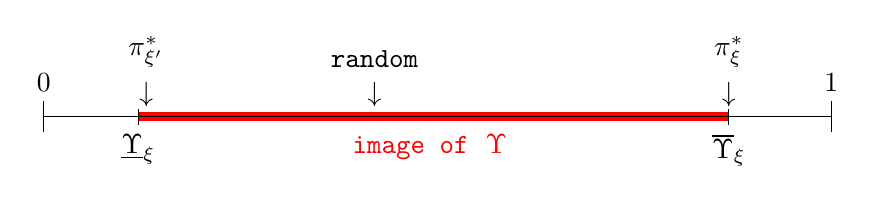
\begin{tikzpicture}
			\filldraw[red] (1.2, .05) -- (8.7, .05) -- (8.7, -.05) -- (1.2, -.05);
			\foreach \x in {2.4, 2.6, 3.5, 4.7, 6.2} {
				%\filldraw[gray] (\x, .05) -- ({\x+.4}, .05) -- ({\x+.4}, -.05) -- (\x, -.05);
			}
			\draw (0,0) to (10, 0);
			\draw (0, -.2) to (0, .2) node[above] {$0$};
			\draw (10, -.2) to (10, .2) node[above] {$1$};
			\draw (4.2, .5) to (4.2, .5) node[above] {\texttt{random}};
			\draw (4.2, 0) to (4.2, 0) node[above] {$\downarrow$};
			\draw (4.2, -.1) to (4.2, -.1) node[below] {\qquad\qquad\textcolor{red}{\texttt{image of}\; $\Upsilon$}};
			\draw (8.7, .1) to (8.7, -.1) node[below] {$\overline\Upsilon_\xi$};
			\draw (8.7, .5) to (8.7, .5) node[above] {$\pi_\xi^*$};
			\draw (8.7, 0) to (8.7, 0) node[above] {$\downarrow$};
			\draw (1.2, .1) to (1.2, -.1) node[below] {$\underline\Upsilon_\xi$};
			\draw (1.3, .5) to (1.3, .5) node[above] {$\pi_{\xi'}^*$};
			\draw (1.3, 0) to (1.3, 0) node[above] {$\downarrow$};
			\end{tikzpicture}
		\end{center}
	\end{figure}
	\centering{Computable policies are dense in $\left[\underline\Upsilon_\xi,\overline\Upsilon_\xi\right]$. \\
		AIXI emulates computable policies.\\
		\Large AIXI can be arbitrarily stupid!}\\
	The devil imitates God. --- \underline{orthogonality}!
	\begin{center}
		\begin{minipage}{.65\textwidth}
			\begin{itemize}
				\item Prior problem in Universal Induction \hfill $\textcolor{red}{\boxed{\checkmark}}$
				\item Prior problem in Universal Intelligence \hfill $\textcolor{red}{\Huge\boxed{\mathbf{!}}}$
			\end{itemize}
		\end{minipage}
	\end{center}
\end{frame}

\begin{frame}\frametitle{Stupid AIXI}
\setlength\abovedisplayskip{0pt}
\setlength\belowdisplayskip{0pt}
	\begin{theorem}[Some AIXIs are Stupid]
		For any Bayesian mixture $\xi$ over $\mathcal{M}_{\mathrm{LSC}}$ and every $\varepsilon> 0$, there is a Bayesian mixture $\xi'$ s.t. $\Upsilon_\xi(\pi_{\xi'}^*)<\underline{\Upsilon}_\xi+\varepsilon$.
	\end{theorem}
	\begin{theorem}[AIXI is Stupid for Some $\Upsilon$]
		For any deterministic $\xi$-optimal policy $\pi_\xi^*$ and for every $\varepsilon> 0$ there is a Bayesian mixture $\xi'$ s.t. $\Upsilon_{\xi'}(\pi_\xi^*)\leq\varepsilon$ and $\overline{\Upsilon}_{\xi'}>1-\varepsilon$.
	\end{theorem}
	\begin{theorem}[Computable Policies can be Smart]
		For any computable policy $\pi$ and any $\varepsilon> 0$ there is a Bayesian mixture $\xi'$ s.t. $\Upsilon_{\xi'}(\pi)>\overline{\Upsilon}_{\xi'}-\varepsilon$.
	\end{theorem}
\end{frame}

\begin{frame}\frametitle{What is a good optimality criterion?}
	\begin{itemize}
		\item Pareto optimality is \textcolor{red}{\emph{trivial}}. Every policy is Pareto optimal in any $\mathcal{M}\supset\mathcal{M}_{\mathrm{comp}}$.
		\item Bayes-optimality is \textcolor{red}{\emph{subjective}}, because two different Bayesians with two different universal priors could view each other's AIXI as a very stupid agent.
	\end{itemize}
\end{frame}

\begin{frame}\frametitle{Optimality}
	\begin{itemize}
		\item Pareto optimality
		\[\nexists\pi': \forall\nu\in\mathcal{M}\left[\left(V_\nu^{\pi'}(\epsilon)\geq V_\nu^\pi(\epsilon)\right)\;\&\;\exists\rho\in\mathcal{M}\left(V_\rho^{\pi'}(\epsilon) > V_\rho^\pi(\epsilon)\right)\right]\]
		\item Balanced Pareto optimality
		\[\forall\pi':\sum\limits_{\nu\in\mathcal{M}} w_\nu\left(V_\nu^\pi(\epsilon)- V_\nu^{\pi'}(\epsilon)\right)\geq 0\]
		\item Bayes optimality($\iff$ Balanced Pareto optimality)
		\[\forall h_{<t}: V_\xi^\pi(h_{<t})=V_\xi^*(h_{<t})\]
		\item Probably approximately correct (PAC)
		\[\forall \varepsilon\delta>0: P_\mu^\pi\left(\forall t\geq m(\varepsilon,\delta): V_\mu^*(h_{<t})-V_\mu^\pi(h_{<t})> \varepsilon\right)<\delta\]
	\end{itemize}
\end{frame}

\begin{frame}\frametitle{Optimality? --- Guess how God created the multiverse}
	\begin{columns}
		\column{.35\textwidth}
			\[\text{prior}\left\{\begin{aligned}
			&\text{distribution}\\
			&\text{hypothesis space}\\
			&\text{\textcolor{yellow}{prior probability}}\\
			&\text{regularization}
			\end{aligned}\right.\]
			
			\centering{\textcolor{red}{No learning without prior!}}\\
			\textcolor{red}{no-free-lunch}
		\column{.4\textwidth}
			\[\left.
			\begin{aligned}
			\text{\textcolor{green}{Homogeneous}}\\
			\text{\textcolor{green}{Causality}}\\
			\text{\textcolor{green}{Simplicity}}\\
			\text{\textcolor{green}{Goodness}}\\
			\text{\textcolor{green}{Beauty}}\\
			\text{\textcolor{green}{Perfection}}\\
			\text{\textcolor{green}{Value}}\\
			\text{\textcolor{green}{Regret}}\\
			\text{\textcolor{green}{Unexpectedness}}\\
			\text{\textcolor{green}{Interesting}}\\
			\textcolor{green}{\cdots}
			\end{aligned}
			\right\rbrace\impliedby\text{\textcolor{green}{God!}}
			\]
	\end{columns}
\end{frame}

\begin{frame}\frametitle{Genesis --- Zero-Sum Two Person Game}
\begin{columns}
\column{.4\textwidth}
\centering\includegraphics[width=\textwidth]{img/ivsgod}
\column{.3\textwidth}
	\begin{figure}[!htbp]
		\includegraphics[width=\textwidth,angle=0,origin=c]{img/centroid}\vspace{-1ex}
		\caption{\textcolor{green}{center of mass}\; \textcolor{yellow}{$\argmax\limits_w\mathbb{E}_w[D(\nu\|\xi)]$}}
	\end{figure}
\end{columns}
	\vspace{-4ex}
	\begin{figure}[!htbp]
		\[\hspace{-1ex}\xrightarrow{\text{message}}\framebox[2cm]{\text{encoder}}\xrightarrow{\mu}\framebox[3cm]{
			$
			\begin{matrix}
			\text{channel}\\
			P(x\mid\nu)\\
			||\\
			\nu(x)
			\end{matrix}
			$
			$
			\begin{bmatrix}
			\nu_1\\
			\nu_2\\
			\vdots\\
			\nu_n\\
			\end{bmatrix}
			$
		}\xrightarrow{x}\framebox[2cm]{\text{decoder}}\xrightarrow{\text{estimated}\atop{\text{message}}}\]\vspace{-2ex}\caption{possible worlds as channel --- dominant strategy equilibrium}
	\end{figure}
\end{frame}

\begin{frame}\frametitle{Genesis --- Zero-Sum Two Person Game}
\centerline{\textcolor{red}{``Subtle is the Lord, but {\Large malicious} He is not.''?}}
\centering\includegraphics[width=.32\textwidth]{img/ivsgod}\vspace*{-3ex}
\begin{itemize}
\item God's strategy: $w$
\item Agent's strategy: $\xi$
\item God's utility: expected redundancy $\mathbb{E}_w[D(\mu\|\xi)]$
\item Agent's utility: $-$ expected redundancy / error bound / channel capacity $\max\limits_wE_w[D(\mu\|\xi)]=\max\limits_w I(\mathcal{M};\mathcal{X})$
\item Nash equilibrium: $(w^*,\xi^*)$ \textcolor{yellow}{dominant strategy equilibrium}
\end{itemize}
\[w^*=\argmax\limits_w I(\mathcal{M};\mathcal{X})\]
\[\xi^*=\argmin\limits_\xi\mathbb{E}_{\textcolor{yellow}{w^*}}\left[D(\mu\|\xi)\right]\]
\[\fbox{\textcolor{red}{The error bound could be arbitrarily large!}}\]
\end{frame}

\begin{frame}\frametitle{Genesis}
	\begin{itemize}
		\item Occam's razor vs Maximum entropy. \[\mathop{minimize}\limits_{w\vDash\left\{
			{\scalebox{.5}{$\begin{aligned}
				& H(w)=C\\
				&\sum\limits_{\nu\in\mathcal{M}}w_\nu=1
				\end{aligned}$}}\right.} \sum\limits_{\nu\in\mathcal{M}}w_\nu K(\nu)\qquad\mathop{maximize}\limits_{w\vDash\left\{
			{\scalebox{.5}{$\begin{aligned}
				&\sum\limits_{\nu\in\mathcal{M}}w_\nu K(\nu)=C\\
				&\sum\limits_{\nu\in\mathcal{M}}w_\nu=1
				\end{aligned}$}}\right.} H(w)\]
		\item Optimal code length for possible worlds --- Solomonoff prior.
		\[\mathop{minimize}\limits_{w\vDash
			\sum\limits_{\nu\in\mathcal{M}}w_\nu=1} \dfrac{\mathbb{E}_w[K]}{H(w)}\]
		\item Maximum expected redundancy/error bound/channel capacity.
		\[\mathop{maximize}\limits_{w\vDash\left\{
			{\scalebox{.5}{$\begin{aligned}
				&H(w)=C\\
				&\sum\limits_{\nu\in\mathcal{M}}w_\nu=1
				\end{aligned}$}}\right.} \mathbb{E}_w\left[D(\nu\|\xi)\right]\qquad\mathop{maximize}\limits_{w\vDash\left\{
			{\scalebox{.5}{$\begin{aligned}
				&\sum\limits_{\nu\in\mathcal{M}}w_\nu K(\nu)=C\\
				&\sum\limits_{\nu\in\mathcal{M}}w_\nu=1
				\end{aligned}$}}\right.} \mathbb{E}_w\left[D(\nu\|\xi)\right]\]
	\end{itemize}
\end{frame}

\begin{frame}\frametitle{What is a good optimality criterion?}
\centering\fbox{\large Asymptotic optimality}
		\begin{itemize}
			\item Asymptotic optimality requires only convergence \textcolor{red}{\emph{in the limit}}.
			\item The agent can be arbitrarily lazy.
			\item \textcolor{red}{AIXI is not asymptotically optimal} because it does not explore enough.
			\item To be asymptotically optimal you have to explore everything.
			\item If you explore more, you're likely to end up in a trap.
			\item Every policy will be asymptotically optimal after falling into the trap.
		\end{itemize}
\begin{figure}[htb]
\subfigure{\includegraphics[height=.2\textwidth]{img/trap1}}
\subfigure{\includegraphics[height=.2\textwidth]{img/trap2}}
\end{figure}
\end{frame}

\begin{frame}\frametitle{}
\begin{block}{}
Agent needs to explore infinitely often for an entire effective horizon.
\end{block}
\[\mathcal{M}\coloneqq \{\nu_\infty,\nu_1,\nu_2,\dots\}\]
\begin{center}
\begin{tabular}{ccc}
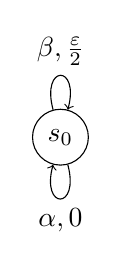
\begin{tikzpicture}[scale=1.2]
\node[circle, draw, minimum height=2em] (s0) at (0, 0) {$s_0$};

\draw[->] (s0) to[loop above] node {$\beta, \frac{\varepsilon}{2}$} (s0);
\draw[->] (s0) to[loop below] node {$\alpha, 0$} (s0);
\end{tikzpicture} & ~~ &
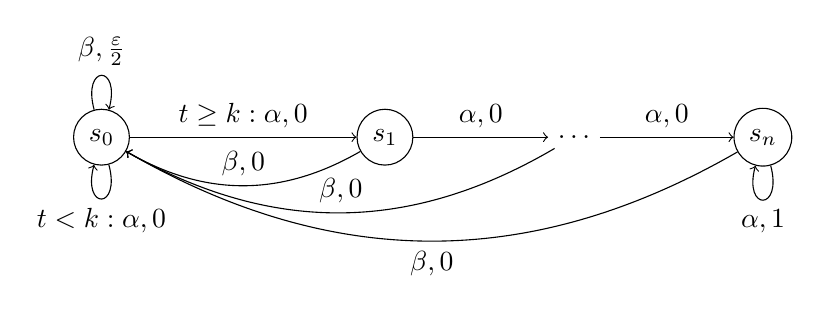
\begin{tikzpicture}[scale=1.2]
\node[circle, draw, minimum height=2em] (s0) at (0, 0) {$s_0$};
\node[circle, draw, minimum height=2em] (s1) at (3, 0) {$s_1$};
\node (ldots) at (5, 0) {$\dots$};
\node[circle, draw, minimum height=2em] (sn) at (7, 0) {$s_n$};

\draw[->] (s0) to[loop above] node {$\beta, \frac{\varepsilon}{2}$} (s0);
\draw[->] (s0) to[loop below] node {$t < k: \alpha, 0$} (s0);
\draw[->] (s0) to node[above] {$t \geq k: \alpha, 0$} (s1);
\draw[->] (s1) to node[above] {$\alpha, 0$} (ldots);
\draw[->] (ldots) to node[above] {$\alpha, 0$} (sn);
\draw[->] (s1) to[bend left] node[above] {$\beta, 0$} (s0);
\draw[->] (ldots) to[bend left] node[above] {$\beta, 0$} (s0);
\draw[->] (sn) to[bend left] node[below] {$\beta, 0$} (s0);
\draw[->] (sn) to[loop below] node {$\alpha, 1$} (sn);
\end{tikzpicture} \\
$\nu_\infty$ && $\nu_k$
\end{tabular}
\end{center}
\end{frame}

\begin{frame}\frametitle{Asymptotic Optimality}
	\begin{itemize}
		\item strongly asymptotically optimal
		\[P_\mu^\pi\left(\lim\limits_{t\to\infty} \left[V_\mu^*(h_{<t})-V_\mu^\pi(h_{<t})\right]=0\right)=1\]
		\item weakly asymptotically optimal
		\[P_\mu^\pi\left(\lim\limits_{n\to\infty} \frac{1}{n}\sum\limits_{t=1}^n\left[V_\mu^*(h_{<t})-V_\mu^\pi(h_{<t})\right]=0\right)=1\]
		\item asymptotically optimal in mean
		\[\lim\limits_{t\to\infty}\mathbb{E}_\mu^\pi\left[V_\mu^*(h_{<t})-V_\mu^\pi(h_{<t})\right]=0\]
		\item asymptotically optimal in probability (PAC)
		\[\forall \varepsilon>0: \lim\limits_{t\to\infty}P_\mu^\pi\left(V_\mu^*(h_{<t})-V_\mu^\pi(h_{<t})>\varepsilon\right)=0\]
	\end{itemize}
	\[\mbox{strong a.o.} \implies
	\begin{cases}
	\mbox{weak a.o.}\\
	\mbox{a.o. in mean} \iff \mbox{a.o. in probability}
	\end{cases}\]
\end{frame}

\begin{frame}\frametitle{AIXI}
	\begin{itemize}
		\item AIXI is not asymptotically optimal.
		\begin{center}
			\resizebox{.9\textwidth}{!}{\fbox{$\forall \mathcal{M}\supset\mathcal{M}_{\mathrm{comp}}\exists\mu\in\mathcal{M}\exists t_0\forall t\geq t_0: P_\mu^{\pi_\xi^*}\left(\lim\limits_{t\to\infty} V_\mu^*(h_{<t})-V_\mu^{\pi_\xi^*}(h_{<t})=\frac{1}{2}\right)=1$}}
		\end{center}
		\item AIXI achieves \textcolor{yellow}{on-policy value convergence}.
		\begin{center}
			\fbox{$P_\mu^\pi\left(\lim\limits_{t\to\infty} V_\mu^\pi(h_{<t})-V_\xi^\pi(h_{<t})=0\right)=1$}
		\end{center}
	Similarly for MDL \textcolor{green}{$\argmin\limits_{\nu\in\mathcal{M}}\{-\log v(e_{<t}\mid a_{<t})+K(\nu)\}$}\\ and universal compression \textcolor{green}{$2^{-Km(e_{<t}\mid a_{<t})}$}.
	\end{itemize}
\textbf{Remark:} AIXI asymptotically learns to predict the environment perfectly and with a small total number of errors analogously to Solomonoff induction, but only on policy: AIXI learns to correctly predict the value of its own actions, but generally not the value of counterfactual actions that it does not take.
\end{frame}

\begin{frame}\frametitle{Effective Horizon}
\setlength\abovedisplayskip{0pt}
\setlength\belowdisplayskip{0pt}
	\[\Gamma_t\coloneqq \sum\limits_{i=t}^\infty\gamma_i\qquad H_t(\varepsilon)\coloneqq \min\left\{m: \dfrac{\Gamma_{t+m}}{\Gamma_t}\leq\varepsilon\right\}\]
	\begin{theorem}
		If there is a nonincreasing computable sequence of positive reals $(\varepsilon_t)_{t\in\mathbb{N}}$ s.t. $\varepsilon_t\xrightarrow{t\to\infty}0$ and $\frac{H_t(\varepsilon_t)}{t\varepsilon_t}\xrightarrow{t\to\infty}0$, then there is a \textcolor{yellow}{limit-computable} policy	that is weakly asymptotically optimal in the class of all computable stochastic environments.
	\end{theorem}
	\begin{definition}[$\varepsilon$-Optimal Policy]
		A policy $\pi$ is $\varepsilon$-optimal in environment $\nu$ iff
		\[\forall h: V_\nu^*(h)-V_\nu^\pi(h)<\varepsilon\]
	\end{definition}
	\centering $\varepsilon$-optimal BayesExp
\end{frame}

\begin{frame}\frametitle{\small Sufficient Condition for Strong Asymptotic Optimality of Bayes}\vspace{-1ex}
	\begin{theorem}[Self-Optimizing Theorem]
		Let $\mu$ be some environment. If there is a policy $\pi$ and a sequence of policies $\pi_1,\pi_2,\dots$ s.t for all $\nu\in\mathcal{M}$
		\begin{equation}
		P_\mu^\pi\left(\lim\limits_{t\to\infty} V_\nu^*(h_{<t})-V_\nu^{\pi_t}(h_{<t})=0\right)=1\label{sao-condition}
		\end{equation}
		then
		\[P_\mu^\pi\left(\lim\limits_{t\to\infty} V_\mu^*(h_{<t})-V_\mu^{\pi_\xi^*}(h_{<t})=0\right)=1\]
	\end{theorem}\vspace{-1ex}
	\begin{itemize}
		\item The policies $\pi_1,\pi_2,\dots$ need to converge to the optimal value on the history generated by $P_\mu^\pi$, not $P_\nu^{\pi_t}$.
		\item If $\pi=\pi_\xi^*$ and (\ref{sao-condition}) holds for all $\mu\in\mathcal{M}$, then $\pi_\xi^*$ is strongly asymptotically optimal in the class $\mathcal{M}$.
		\item \textcolor{yellow}{$\pi_\xi^*$ is strongly asymptotically optimal in the class of ergodic finite-state MDPs if $\forall \varepsilon: H_t(\varepsilon)\xrightarrow{t\to\infty}\infty$.}
	\end{itemize}
\end{frame}

\begin{frame}\frametitle{For Which Class $\mathcal{M}$ does $V_\mu^{\pi_\xi^*}$ Converge to $V_\mu^*$?}
	\begin{figure}
	\includegraphics[width=.7\textwidth,angle=0,origin=c]{img/self-optimising}
	\end{figure}
\end{frame}

\begin{frame}\frametitle{Recoverability}
	An environment $\nu$ is recoverable iff
	\[\lim\limits_{t\to\infty}\sup\limits_\pi\Big|\mathbb{E}_\nu^{\pi_\nu^*}\left[V_\nu^*(h_{<t})\right]-\mathbb{E}_\nu^\pi\left[V_\nu^*(h_{<t})\right]\Big|=0\]
	\textbf{Remark:} Recoverability compares following the worst policy $\pi$ for $t-1$ time steps and then
	switching to the optimal policy $\pi_\nu^*$ to having followed $\pi_\nu^*$ from the beginning. The recoverability assumption states that switching to the optimal policy at any time enables the recovery of most of the value.
\end{frame}

\begin{frame}\frametitle{Sublinear Regret}\vspace{-1ex}
\setlength\abovedisplayskip{0pt}
\setlength\belowdisplayskip{0pt}
	\[R_m(\pi,\mu)\coloneqq \sup\limits_{\pi'}\mathbb{E}_\mu^{\pi'}\left[\sum\limits_{t=1}^m r_t\right]-\mathbb{E}_\mu^\pi\left[\sum\limits_{t=1}^m r_t\right]\]
	\begin{assumption}[Discount Assumption]
		\begin{enumerate}
			\item $\forall t:\gamma_t>0$
			\item $\gamma_t$ is monotone decreasing.
			\item $\forall \varepsilon>0: H_t(\varepsilon)\in o(t)$
		\end{enumerate}
	\end{assumption}\vspace{-1ex}
	\begin{theorem}
		If the discount function $\gamma$ satisfies the discount assumption, the environment $\mu$ is recoverable, and $\pi$ is asymptotically optimal in mean, then $R_m(\pi,\mu)\in o(m)$.
	\end{theorem}\vspace{-1ex}
	\[\argmin\limits_\pi\max\limits_\mu R_m(\pi,\mu)\qquad\qquad w_m^\mu\coloneqq \frac{2^{-R_m(\pi,\mu)}}{\sum\limits_{\mu\in\mathcal{M}}2^{-R_m(\pi,\mu)}}\]
\end{frame}

\begin{frame}\frametitle{Regret in Non-Recoverable Environments}
	\begin{figure}
		\includegraphics[width=.7\textwidth,angle=0,origin=c]{img/hell-heaven}
	\end{figure}
\[R_m(\alpha,\mu_1)=m\qquad R_m(\alpha,\mu_2)=0\]
\[R_m(\beta,\mu_1)=0\qquad R_m(\beta,\mu_2)=m\]
	\begin{block}{}
		For non-recoverable environments:\\
		\textcolor{red}{Either the agent gets caught in a trap or it is not asymptotically optimal.}
	\end{block}
\end{frame}

\begin{frame}\frametitle{}
\begin{figure}
	\includegraphics[width=.75\textwidth,angle=0,origin=c]{img/beauty.png}
\end{figure}
\end{frame}

\begin{frame}\frametitle{\href{https://arxiv.org/abs/1411.1373}{Hibbard's Two-Stage Model-Based Utility Agent}}
\begin{align*}
&\lambda(h)\coloneqq \argmax\limits_{q\in\mathcal{Q}} P(h\mid q)P(q)\\
&\rho(h')=P(h'\mid \lambda(h))\\
&Q(ha)=\sum\limits_{e\in\mathcal{E}}\rho(e\mid ha)\left[\sum\limits_{z\in Z_h}P(z\mid \lambda(h))u(z)+\gamma V(h\ae)\right]\\
&V(h)=\max\limits_{a\in\mathcal{A}}Q(ha)\\
&\pi(h)=\argmax\limits_{a\in\mathcal{A}}Q(ha)
\end{align*}
where $Z_h$ is the internal state histories induced by $\lambda(h_{<t})$ that are consistent with $h$.

\textbf{Remarks:} An agents using \textcolor{yellow}{model-based utility function} will not self-delude: it need to make more accurate estimate of its environment state variables from its interaction history.
\end{frame}

\begin{frame}\frametitle{Russell's Principles for Beneficial Machines}
\begin{enumerate}
	\item The machine's only objective is to maximize the realization of human preferences.
	\item The machine is initially uncertain about what those preferences are.
	\item The ultimate source of information about human preferences is human behavior.
\end{enumerate}
\end{frame}

\begin{frame}\frametitle{Reward-Modeling}
\begin{figure}[H]
\includegraphics[width=.7\textwidth]{img/reward-model.png}
\end{figure}
\end{frame}

\begin{frame}\frametitle{Reward-Modeling}
\begin{figure}
\tikzstyle{block} = [rectangle, draw, text width=8em, text centered, rounded corners, minimum height=4em]
\begin{tikzpicture}[node distance = 6em, auto, thick]
\node [block] (policy) at (0, 0) {agent $A_k$};
\node [block] (environment) at (6, 0) {environment};
\node [block] (reward model) at (0, 3) {reward model};
\node [block] (user) at (6, 3) {user};
\node [block] (prevpolicy) at (6, 5.5) {agent $A_{k-1}$};

\draw[->] (environment.170) to node[above] {observation} (policy.10);
\draw[->] (environment.170) to (reward model.-20);
\draw[->] (environment) to node[right] {trajectories} (user);
\draw[->] (user) to node[above] {feedback} (reward model);
\draw[->] (reward model) to node[left] {reward} (policy);
\draw[->] (policy.-10) to node[below] {action} (environment.190);

\draw[->] (user.80) to node[right] {interaction} (prevpolicy.-80);
\draw[->] (prevpolicy.-100) to (user.100);
\end{tikzpicture}
\end{figure}	
\end{frame}

\begin{frame}\frametitle{Daniel Dewey's Value Learning Agent \& CIRL}
\[a_k^*=\argmax\limits_{a_k}\sum\limits_{e_k\ae_{k+1:m}}\xi(\ae_{\leq m}\mid \ae_{<k}a_k)\sum\limits_{u\in\mathcal{U}}P(u\mid \ae_{\leq m})u(\ae_{\leq m})\]
What could it mean for a machine to have its own goals?
\[\text{\textcolor{red}{Shutdown Button} --- Uncertainty of goals}\]
\[\tilde{U}(u)\implies P_{\tilde{U}}(u)\]
Russell: Cooperative Inverse Reinforcement Learning

CIRL agents learn about a human utility function $u^*$ by observing the actions the human takes.
\resizebox{\textwidth}{!}{\begin{minipage}{1.05\textwidth}
\[V^*(\ae_{<k})=\max\limits_{a_k\in\mathcal{A}}Q^*(\ae_{<k}a_k)\]
\[Q^*(\ae_{<k}a_k)=\mathbb{E}_{e_k}\left[\textcolor{yellow}{\sum\limits_{a_k^H}P(a_k^H\mid a_k)\sum\limits_{u\in\mathcal{U}}P(u\mid a_k,a_k^H)u(\ae_{1:k})}+\gamma V^*(\ae_{1:k})\,\middle|\,\ae_{<k}a_k\right]\]
\end{minipage}}
\end{frame}

%--------------------------%
\subsection{Leibniz}
%--------------------------%

\begin{frame}\frametitle{Leibniz 1646-1716}
	\begin{columns}
		\column{0.57\textwidth}
			\begin{block}{}
				\centerline{\Large Don't argue. Calculate!}
			\end{block}
			\begin{itemize}
				\item \textcolor{green}{{\small Principle of Contradiction}}: Nothing can be and not be, but everything either is or is not. (Everything that is not self-contradictory is possible.)
				\item \textcolor{green}{{\small Principle of Sufficient Reason}}: Nothing happens without a reason why it should be so rather than otherwise.
				\item \textcolor{yellow}{{\small Principle of Perfection}}: The real world is the best of all possible worlds.
			\end{itemize}
			\begin{block}{In the beginning was the Logic.}
				As God calculates, so the world is made.
			\end{block}
		\column{0.23\textwidth}
			\begin{figure}
				\includegraphics[width=\textwidth,angle=0,origin=c]{img/leibniz0.jpg}
			\end{figure}
	\end{columns}
\end{frame}

\begin{frame}\frametitle{As God calculates, so the world is made.}
\begin{figure}
	\includegraphics[width=\textwidth,angle=0,origin=c]{img/godprogram.jpg}
\end{figure}
\end{frame}

\begin{frame}\frametitle{Leibniz}
	\begin{itemize}
		\item The last ``universal genius'', developed Calculus, refined binary number system, invented mechanical calculator that could perform addition, subtraction, multiplication and division.
		\item Leibniz was claimed (by Russell, Euler, G\"odel, Weiner, Mandelbrot, Robinson, Chaitin) to be a precursor of \emph{mathematical logic, topology, game theory, cybernetic theory, fractal geometry, non-standard analysis, algorithmic information theory and digital philosophy}.
		\item Wolfram: ``Leibniz had the idea of encoding logical properties using numbers. He thought about associating every possible attribute of a thing with a prime number, then characterizing the thing by the product of the primes for its attributes --- and then representing logical inference by arithmetic operations.''
		%\item Diderot: ``When one compares the talents one has with those of a Leibniz, one is tempted to throw away one's books and go die quietly in the dark of some forgotten corner.''
	\end{itemize}
\end{frame}

\begin{frame}\frametitle{Leibniz's Monadology: Possible Worlds $\to$ Real World}
\begin{itemize}
	\item The genuine substance is monad.
	\item Monads are incorporeal automata.
	\item Each monad strive for existence with its \emph{propensity} and hence will exist unless other monads prevent it, which also demand existence and are incompatible with it.
	\item As there are infinitely many different combinations of possibles, there are infinitely many \emph{possible worlds}.
	\item All possibles strive with equal right for existence in proportion to the \emph{degree of perfection} they contain.
	\item The real world is the best of all possible worlds, with the greatest \emph{resultant perfection}.
\end{itemize}
\end{frame}

\begin{frame}\frametitle{Leibniz's Principle of Perfection}
\textbf{Question:} Why things have turned out so rather than otherwise?
\begin{quote}
``All natural phenomena could be explained mechanically, but the principles of mechanics themselves cannot be so explained. They depend on more substantive principles. The final analysis of the laws of nature leads us to the most sublime \textbf{Principle of Perfection} --- the real world is the best of all possible worlds. \textcolor{yellow}{It is wrong that laws are entirely indifferent, since they originate in the principle of greatest perfection.}''

``\textcolor{green}{When a rule is extremely complex, that which conforms to it passes for random.} No matter how God might have created the world, it would always have been regular. God has chosen that world which is the most perfect, that is to say, which is at the same time \textcolor{yellow}{the simplest in its hypotheses and the richest in phenomena.}''\par
\hfill --- \textsl{Leibniz}
\end{quote}
\end{frame}

\begin{frame}\frametitle{Monadology: ``Physical'' World}
\begin{block}{Physical World is an Illusion}
Each monad has a derived position in the sense that its point of view is ``located'' in one ``place'' rather than
another. Each monad's point of view can be mapped with other monads' points of view into a single sort of hologram. When a monad experiences a collection of ``pixels'' on its screen, it interprets the collection as some ``physical object'', and when other monads do the same their perceptions are ``veridical''. If one monad's point of view doesn't map onto the points of view of others, it is experiencing a hallucination. The so-called ``physical world'' is situated in the harmony perceptions of monads. Corporeal matter is nothing but a logical construction of the perceptions of monads. Time and space are not things, but orders of things.	
\end{block}
\end{frame}

\begin{frame}\frametitle{Monadology: Variety}
\begin{block}{What is ``Variety''?}
``Monads reflect the same world from their own point of view. This interconnection, or this adapting of all the monads to each one, and of each one to all the others, brings it about that each monad has relational properties that express all the others, so that each monad is a perpetual living mirror of the world. Just as the same town when seen from different sides will seem quite different --- as though it were multiplied perspectively. And \emph{that is the way to get the greatest possible \textcolor{red}{variety}}, but with all the order there could be; i.e. \emph{it is the way to get as much perfection as there could be.}''	
\end{block}
\begin{itemize}
	\item Variety: expected codeword length of the experience of all the monads
	\item Simplicity: optimal codeword length of the experience
\end{itemize}
\end{frame}

\begin{frame}\frametitle{Leibniz's Philosophy of Deductive Logic}
		\begin{enumerate}[1]
			\item Characteristica Universalis \& Calculus Ratiocinator.
			\begin{enumerate}[i]
				\item \textcolor{green}{the coordination of knowledge in an encyclopedia} --- collect all present knowledge so we could sift through it for what is fundamental. With the set of ideas that it generated, we could formulate the \emph{characteristica universalis}. (which form the alphabet of human thought).
				\item \emph{\textbf{characteristica universalis}} --- a \textcolor{green}{universal ideal language} whose rules of composition directly expresses the structure of the world.
					\[\textcolor{yellow}{\text{sign}\rightleftarrows\text{idea}}\]
					\begin{center}
						{\footnotesize \textcolor{yellow}{
								encyclopedia $\Rightarrow$ fundamental principles $\Rightarrow$ primitive notions}}
					\end{center}
				\item \emph{\textbf{calculus ratiocinator}} --- the arrangement of \textcolor{green}{all true propositions} in an \textcolor{green}{axiomatic system}.
				\item \textcolor{green}{decision procedure}. --- an algorithm which, when applied to any formula of the \emph{characteristica universalis}, would determine whether or not that formula were true. \textcolor{red}{--- a procedure for the rapid enlargement of knowledge. replace reasoning by computation. the art of invention. free mind from intuition.}
				\item a proof that the \emph{calculus ratiocinator} is \textcolor{green}{consistent}.
			\end{enumerate}
		\end{enumerate}
\end{frame}

\begin{frame}\frametitle{\href{https://philpapers.org/rec/HACTLP}{Leibniz's Philosophy of Inductive Logic / Probability}}
		\begin{figure}
			\includegraphics[width=0.23\textwidth,angle=0,origin=c]{img/overfitting.pdf}
		\end{figure}
		\vspace{-7pt}
	\begin{enumerate}\setcounter{enumi}{1}
			\item Compute all descriptions of possible worlds that can be expressed with the primitive notions. And the possible worlds will all have some propensity to exist.
			\item Compute the probabilities of disputed hypotheses relative to the available data. As we learn more our probability assignments will asymptotically tend to a maximum for the real world, i.e. the possibility with the highest actual propensity.
		\end{enumerate}
\begin{itemize}
		\item ``Probability is degree of possibility (perfection).''
		\item ``A hypothesis is more probable as it is simpler to understand and wider in explanatory power.''
	\end{itemize}
	\[\large\textcolor{red}{\mbox{probability} = \mbox{propensity} \propto \mbox{perfection} = f(\mbox{variety},\mbox{simplicity})}\]
\end{frame}

\begin{frame}\frametitle{Leibniz's Philosophy of Mind}
\centerline{\hspace*{-1ex}\fbox{bare monad $\xrightarrow[\textcolor{red}{\text{long memory}}]{\textcolor{red}{\text{perception}}}$ soul $\xrightarrow[\textcolor{red}{\text{abstraction}}]{\textcolor{red}{\text{consciousness}}}$ mind $\xrightarrow{\textcolor{red}{\text{Supreme Perfection}}}$ God}}
	\begin{itemize}
		\item \textbf{perception} $=$ the internal representation of the external world
		\item \textbf{consciousness} $=$ the reflective knowledge of the perception
	\end{itemize}
	\begin{itemize}
		\item A \textbf{soul} is a living substance. ``Every living substance is made up of smaller living substances which in their turn are made up of still smaller ones, and so on down to infinity. There are infinite levels of life among monads, some of which are more or less dominant over others.''
		\item ``Our knowledge of necessary truths, and our grasp of the abstractions they involve, raise us to reflexive acts, which make us aware of the thing that is called `I'.''
		\item ``Every substance represent the whole world in its own way, as if in a world apart, and as if there existed only God and itself.''
	\end{itemize}
\end{frame}

\begin{frame}\frametitle{Leibniz's Philosophy of Mind}
\begin{table}
\abovetabulinesep=1mm
\belowtabulinesep=1mm
\begin{tabu}{p{.1\textwidth}|p{.25\textwidth}|p{.25\textwidth}|p{.25\textwidth}}
\hline
 & \textbf{example} & \textbf{perception} & \textbf{appetite} \\
\hline
\textbf{bare monad} & monads in inanimate objects & unconscious perception & unconscious appetite \\
\hline
\textbf{soul} & central monads of animals & sensible perception & sensible appetite \\
\hline
\textbf{mind} & central monads of human beings & rational perception: reflective knowledge of the perception & rational appetite: aware of the appetite and understand why we have it \\
\hline
\end{tabu}
\end{table}
\textbf{Free Will:} acting freely requires acting in accordance with one's rational assessment of which course of action is best. It requires both knowledge of rational judgments about the good, as well as the tendency to act in accordance with these judgments.
\end{frame}

\begin{frame}\frametitle{Free Will}
\begin{itemize}
		\item ``Indifference arises from ignorance, and the wiser a man is, the more determined he is toward the most perfect.''
		\item ``Monads are freer in proportion as they are further removed from indifference and more self-determined...Now in so far as we have lights, and act according to reason, we shall be determined by the perfections of our own nature, and consequently we shall be freer in proportion as we are less embarrassed as to our choice...Let us not pretend to that harmful liberty, of being in uncertainty and perpetual embarrassment, like that Ass of Buridan, who, being placed at an equal distance between two sacks of wheat, and having nothing that determined him to go to one rather than the other, allowed himself to die of hunger.''
		\item ``The more monads are determined by themselves, and removed from indifference, the more perfect they are.''
\begin{align*}
\textcolor{red}{\mbox{free}} & \textcolor{red}{\mbox{ will} \propto \mbox{perfection} = f(\mbox{variety},\mbox{simplicity})}\\
&\textcolor{red}{\Uparrow} \\
\textcolor{red}{\textit{do actions to be}}\;& \textcolor{red}{\mbox{removed from indifference}}
\end{align*}
	\end{itemize}	
\end{frame}

\begin{frame}\frametitle{Buridan's Ass}
\begin{figure}[H]
\includegraphics[width=.5\textwidth]{img/buridan-ass.jpg}
\end{figure}
``There are no two individuals indiscernible from each other, because if there were, God and nature would act without reason.''
\end{frame}

\begin{frame}\frametitle{Leibniz's Philosophy of Happiness}
\begin{itemize}
	\item ``The games mixed of chance and combinations represent human life.''
	\item ``Wisdom is the science of achieving happiness.''
	\item ``Happiness is a lasting state of pleasure.''
	\item ``Pleasure is a sense of perfection that results from everything the soul feels at once.''
	\item ``An intelligent being's pleasure is simply the perception of beauty, order and perfection.''
	\item ``The Supreme happiness of man consists in the greatest possible increase of his perfection.''
\end{itemize}	
\end{frame}

\begin{frame}\frametitle{Leibniz's Philosophy of Happiness}
\begin{itemize}
	\item ``To love is to find pleasure in the perfection of others.''
	\item God has the greatest perfection.
	\item ``As we would only know God through his emanations, there are two ways of seeing his perfection, namely
	\begin{enumerate}
		\item in the knowledge of eternal truths, explaining the reasons in themselves,
		\item in the knowledge of the harmony of the universe, by applying reasons to experiences.
	\end{enumerate}
	That is to say, we must know the wonders of reason and the wonders of nature.'' (MDL?)
	\item ``The more a mind desires \emph{to know order}, reason, the beauty of things which God has produced, and the more it is moved \emph{to imitate this order} in the things which God has left to its management, the happier it will be.''
\end{itemize}
\end{frame}

\begin{frame}\frametitle{What is Perfection?}
\begin{block}{God --- The Creator / Architect / Monarch}
It follows from the \textbf{supreme perfection} of God, that in creating the universe He has chosen the best possible plan, in which there is
\begin{enumerate}
\item the greatest \textcolor{red}{variety} along with the greatest \textcolor{red}{order};\hfill \textcolor{green}{--- metaphysical}
\item the best arranged situation, space and time;\hfill \textcolor{green}{--- physical}
\item the maximum \textcolor{red}{effect} produced by the simplest \textcolor{red}{means};\hfill \textcolor{green}{--- metaphysical}
\item the highest levels of power, knowledge, \textcolor{red}{happiness} and goodness in the creatures that the universe could allow.\hfill \textcolor{green}{--- moral}
\end{enumerate}
\end{block}
\end{frame}

\begin{frame}\frametitle{Pre-established Harmony}
\begin{itemize}
	\item ``Monads have no windows.''
	\item ``A monad's perceptions arise out of its other perceptions by the
	\begin{itemize}
		\item laws of appetites --- the \textbf{laws of the final causes} of good and evil,
	\end{itemize}
	just as changes in bodies or in external phenomena arise one from another by the
	\begin{itemize}
		\item \textbf{laws of efficient causes} --- the laws governing the movements of bodies.
	\end{itemize}
	So there is perfect harmony between the perceptions of the monad and the movements of bodies, a \textbf{harmony that was pre-established} from the outset between the system of final causes and that of efficient causes.''
	\item ``Souls act according to the laws of final causes through appetitions, ends, and means. Bodies act according to the laws of efficient causes or motions. And the two realms, that of efficient causes and that of final causes, are in harmony with one another.''
\end{itemize}
\end{frame}

\begin{frame}\frametitle{Leibniz's Program}
\begin{figure}
	\includegraphics[width=\textwidth,angle=0,origin=c]{img/leibnizprogram-cn}
\end{figure}
\end{frame}

\begin{frame}\frametitle{Leibniz Prior}
\begin{itemize}
	\item There's much we don't know about the world.
	\item but we know it's the best possible world.
	\item So \textcolor{yellow}{simplicity and richness} will be represented in the actual (best possible) world.
	\item This is a good \textcolor{red}{inductive bias}.
\end{itemize}
\end{frame}

\begin{frame}\frametitle{Leibniz Prior}
	\begin{columns}[onlytextwidth]
		\column{0.47\textwidth}
			\begin{itemize}
				\item the best of all possible worlds
				\item balancing the \textcolor{yellow}{simplicity of means} against the \textcolor{yellow}{richness of ends}
				\item pre-established harmony
			\end{itemize}
			\begin{center}
				\textcolor{red}{prior}\\
				$\Downarrow$\\
				\textcolor{yellow}{utility}\\
				$\Downarrow$\\
				\textcolor{red}{prior}
			\end{center}
	\centerline{Orthogonality!}
	\centerline{Wisdom $\ne$ Intelligence}
		\column{0.53\textwidth}
			\begin{gather*}
			\textcolor{red}{{\text{universal prior (assumption)}}~w}\\
			\MapDown{\textcolor{yellow}{\text{simplicity/richness}}}\\
			\textcolor{yellow}{\text{intrinsic utility}}\\
			\MapDown{\text{stochastic environment}}\\
			\text{expected intrinsic utility}\\
			\MapDown{\textcolor{green}{\underline{\text{Schauder fixpoint}}}}\\
			\textcolor{red}{{\text{universal prior}}~w^*}\\
			\MapDown{\text{Bayesian mixture}}\\
			\xi\\
			\MapDown{\text{ExpectiMax}}\\
			\pi_\xi^*
			\end{gather*}
	\end{columns}
\end{frame}

\begin{frame}\frametitle{}
\begin{quote}
\begin{itemize}
	\item Without mathematics one cannot understand the fundamentals of philosophy.
	\item Without philosophy we cannot reach the foundation of mathematics.
	\item Without both (mathematics and philosophy) one cannot reach anything that is fundamental.
\end{itemize}\par
\hfill --- \textsl{Leibniz}
\end{quote}
\begin{quote}
``There is nothing that can be said by mathematical symbols and relations which cannot also be said by words.\\
The converse, however, is false.\\
\textcolor{green}{Much that can be and is said by words cannot be put into equations,} \textcolor{red}{because it is nonsense.}''\par
\hfill --- \textit{Clifford Truesdell}
\end{quote}
\end{frame}

\begin{frame}\frametitle{Leibniz's ``Wisdom''}
\[\underline{W}isdom=\argmax\limits_\pi \mathbb{E}_\xi^\pi[\underline{H}appiness]\]
\[\underline{H}appiness=\sum\limits_{t=1}^\infty \underline{P}erfection(t)\]
\[\underline{P}erfection=\underline{V}ariety-\underline{S}implicity\]
\[\underline{V}ariety=\mathbb{E}_w[\underline{P}erception]\]
\[\underline{P}erception=\underline{R}eason + (\underline{E}xperience\mid\underline{R}eason)\]
\[\pi^*\coloneqq \argmax\limits_\pi\mathbb{E}_\xi^\pi\left[\sum\limits_{t=1}^\infty\Big(\mathbb{E}_w\left[R + (E\mid R)\right] - S\Big)\right]\]
\begin{quote}
The understanding of mathematics is necessary for a sound grasp of ethics.\par
\hfill --- \textsl{Socrates}
\end{quote}
\end{frame}

\begin{frame}\frametitle{Leibniz's ``Wisdom''}
\[u^{\mathrm{in}}(h_{1:t})=H(w_\epsilon)-H(w_{h_{1:t}})\quad\mbox{or}\quad D(w_{h_{1:t}}\|w_\epsilon)-D(w_\epsilon\|w_{h_{1:t}})\]
\[\bar{U}(\nu)=\mathbb{E}_\nu\left[\sum\limits_{t\geq 1} u^{\mathrm{in}}(h_{1:t})\right]\]
\[w_\epsilon^\nu\mapsto\bar{U}(\nu)\mapsto w_\epsilon^\nu\]
\[
\pi^*\coloneqq \argmax\limits_\pi\mathbb{E}_\xi^\pi\left[\sum\limits_{t=1}^\infty u^{\mathrm{in}}(h_{1:t})\right]
\]
\end{frame}

\begin{frame}\frametitle{}
	\begin{itemize}
		\item \underline{Prior: Simplicity}(Kolmogorov Complexity) $\xrightarrow[\text{regular/random}~\mathcal{M}]{\text{break block uniform}}$ free lunch
		\item \underline{\textcolor{green}{Intrinsic Utility}}
		\item \underline{Universal Prior} (Natural UTM)
	\end{itemize}
		\centering\textcolor{green}{Metaphysical} vs \textcolor{green}{Moral/Utilitarian} \\
		means vs ends \qquad wisdom vs intelligence
	\[\textcolor{green}{\mbox{simplicity/richness}\to\mbox{intrinsic utility}\to\mbox{universal prior}}\]
	\[\mbox{inverse/value reinforcement learning}\]\vspace{-3ex}
\begin{columns}
\column{0.37\textwidth}
	\begin{itemize}
		\item \textcolor{yellow}{\textbf{orthogonality}}
		\item \textbf{human interests}
		\item \textcolor{red}{\textbf{external wireheading}}
		\item \textcolor{red}{\textbf{shutdown button}}
	\end{itemize}
\column{0.23\textwidth}
	\begin{figure}[H]
		\begin{center}
			\includegraphics[width=\textwidth,angle=0,origin=c]{img/walle-fire}\\
			\includegraphics[width=\textwidth,angle=0,origin=c]{img/walle-rubik}
		\end{center}
	\end{figure}
\column{0.2\textwidth}
	\begin{figure}[H]
		\begin{center}
			\includegraphics[width=\textwidth,angle=0,origin=c]{img/wireheading}
		\end{center}
	\end{figure}
\column{0.2\textwidth}
	\begin{figure}[H]
		\begin{center}
			\includegraphics[width=\textwidth,angle=0,origin=c]{img/button}
		\end{center}
	\end{figure}
\end{columns}
\end{frame}

%--------------------------%
\subsection{Variants of AIXI}
%--------------------------%

\begin{frame}\frametitle{\href{http://www.hutter1.net/publ/ksaprob.pdf}{Knowledge-Seeking Agent}}\vspace{-2ex}
	\[
	V_{\mathrm{IG}}^{\pi,m}(h_{<t})\coloneqq \mathbb{E}_\xi^\pi\left[\textcolor{yellow}{H\big(w_{h_{<t}}^\cdot\big)-H\big(w_{h_{1:m}}^\cdot\big)}\,\middle|\, h_{<t}\right]=\sum\limits_{\nu\in\mathcal{M}} w_{h_{<t}}^\nu D_m\big(P_\nu^\pi\big\|P_\xi^\pi\bigm\vert h_{<t}\big)
	\]
\begin{gather*}
	D_\gamma\big(P_\nu^\pi\big\|P_\xi^\pi\bigm\vert h_{<t}\big)\coloneqq \sum\limits_{k=t}^\infty\gamma_k\sum\limits_{h'\in\mathcal{H}^{k-t}}P_\nu^\pi(h'\mid h_{<t})D\big(P_\nu^\pi\big\|P_\xi^\pi\bigm\vert h_{<t}h'\big)\\
	V_{\mathrm{IG}}^\pi(h_{<t})\coloneqq \mathbb{E}_\xi^\pi\left[\sum\limits_{k=t}^\infty\gamma_k \textcolor{yellow}{D\big(w_{h_{1:k}}^\cdot\big\| w_{h_{<k}}^\cdot\big)}\,\middle|\, h_{<t}\right]=\sum\limits_{\nu\in\mathcal{M}}w_{h_{<t}}^\nu D_\gamma\big(P_\nu^\pi\big\|P_\xi^\pi\bigm\vert h_{<t}\big)\\
	\pi_{\mathrm{IG}}^*\coloneqq \argmax\limits_\pi V_{\mathrm{IG}}^\pi
\end{gather*}
	\[\lim\limits_{t\to\infty}\frac{1}{\Gamma_t}\mathbb{E}_\mu^\pi\left[D_\gamma\big(P_\mu^\pi\big\|P_\xi^\pi\bigm\vert h_{1:t}\big)\right]=0 \tag{on-policy}\]
	\[\lim\limits_{t\to\infty}\frac{1}{\Gamma_t}\mathbb{E}_\mu^{\pi_{\mathrm{IG}}^*}\left[\sup\limits_{\pi\in\Pi(h_{1:t})}D_\gamma\big(P_\mu^\pi\big\|P_\xi^\pi\bigm\vert h_{1:t}\big)\right]=0 \tag{off-policy}\]
	\resizebox{\textwidth}{!}{maximize knowledge / exploration$=$exploitation / resistant to noise / avoid traps}
\end{frame}

\begin{frame}\frametitle{\href{http://www.aslanides.io/aixijs/}{Bayesian Agent}}
\begin{algorithm}[H]
\begin{algorithmic}[1]
\Require{Model class $\mathcal{M}$; prior $w\in\Delta\mathcal{M}$; history $\ae_{<t}$.}
%\Statex
\Function{act}{$\pi$}
\State Sample and perform action $a_t\sim \pi(\cdot\lvert \ae_{<t})$
\State Receive $e_t\sim \nu(\;\cdot\;\lvert \ae_{<t}a_t) $
\For{$\nu\in\mathcal{M}$}
\State $w_\nu \gets \frac{\nu\left(e_{<t}\lvert a_{<t}\right)}{\xi\left(e_{<t}\lvert a_{<t}\right)}w_\nu$
\EndFor
\State $t \gets t + 1$
\EndFunction
\end{algorithmic}
\caption{Bayesian Agent}\label{alg:bayesian}
\end{algorithm}
\end{frame}

\begin{frame}\frametitle{MDL}
\begin{algorithm}[H]
\begin{algorithmic}[1]
\Require{Model class $\mathcal{M}$; prior $w\in\Delta\mathcal{M}$; regularizer constant $\lambda\in\mathbb{R}^+$.
}
%\Statex
\Loop
\State $\sigma\gets\arg\min_{\nu\in\mathcal{M}}\left[K(\nu) - \lambda\sum\limits_{k=1}^{t}\log\nu(e_k\mid\ae_{<k}a_k)\right]$
\State $\textsc{act}\left(\pi_{\sigma}^*\right)$
\EndLoop
\end{algorithmic}
\caption{MDL Agent}\label{alg:mdl}
\end{algorithm}
\end{frame}

\begin{frame}\frametitle{MDL}
\setlength\abovedisplayskip{0pt}
\setlength\belowdisplayskip{0pt}
	\begin{definition}[MDL]
		\[ \widehat{\nu}=\arg\min\limits_{\nu\in\mathcal{M}}\{K_\nu(x)+K_w(\nu)\}=\arg\max\limits_{\nu\in\mathcal{M}}\{w_\nu \nu(x)\}\]
		where $K_\nu(x)\coloneqq -\log\nu(x)$ and $K_w(\nu)\coloneqq -\log w_\nu$
	\end{definition}
	\begin{theorem}[MDL Bound]
		\begin{gather*}
		\sum\limits_{t=1}^\infty\mathbb{E}_\mu\left[\sum\limits_{x_t\in\mathcal{X}}\Big(\widehat{\nu}(x_t\mid x_{<t})-\mu(x_t\mid x_{<t})\Big)^2\right]
		\leqa 8w_\mu^{-1}
		\end{gather*}
	\end{theorem}
	MDL converges, but speed can be exponential worse than Bayes.
\end{frame}

\begin{frame}\frametitle{Weak Asymptotic Optimality --- Optimistic Agent}\vspace{-1ex}
\begin{algorithm}[H]
\begin{algorithmic}[1]
\Require{Finite class of deterministic environments $\mathcal{M}_0=\mathcal{M}$}
\State $t=1$
\Repeat
\State $(\pi^*,\nu^*)\coloneqq \argmax_{\pi\in\Pi,\nu\in\mathcal{M}_{t-1}}V_\nu^\pi(h_{t-1})$
 \Repeat
 \State $a_t=\pi^*(h_{t-1})$
 \State Perceive $e_t$ from environment $\mu$
 \State $h_t\gets h_{t-1}a_te_t$
 \State Remove inconsistent environment $\mathcal{M}_t\coloneqq \left\{\nu\in\mathcal{M}_{t-1}: h_t^{\pi^\circ\nu}=h_t\right\}$
 \State $t\gets t+1$
 \Until $\nu^*\notin\mathcal{M}_{t-1}$
\Until $\mathcal{M}=\emptyset$
\end{algorithmic}
\caption{Optimistic Agent $\pi^\circ \hfill \pi_t^\circ\coloneqq \argmax_\pi\max_{\nu\in\mathcal{M}_t} V_\nu^\pi(h_{1:t})$}\label{alg:optimistic}
\end{algorithm}\vspace{-1ex}
	stochastic case: $\mathcal{M}_t\coloneqq \Big\{\nu\in\mathcal{M}_{t-1}: \nu(e_{<t}\mid a_{<t})\geq\varepsilon_t\max\limits_{\rho\in\mathcal{M}}\rho(e_{<t}\mid a_{<t})\Big\}$\\
	Act optimally w.r.t. the most optimistic environment until contradicted.\\
	If there is a chance: Try it! --- Vulnerable to traps.
\end{frame}

\begin{frame}\frametitle{\href{https://jan.leike.name/}{Asymptotic Optimality in Mean --- Thompson Sampling}}
\begin{algorithm}[H]
\begin{algorithmic}[1]
\Require{Model class $\mathcal{M}$; prior $w\in\Delta\mathcal{M}$; exploration schedule $\left(\varepsilon_t\right)_{t\in\mathbb{N}}$.
}
%\Statex
\Loop
\State Sample $\rho\sim w_{\ae_{<t}}^\cdot$
\For{$i=1\to H_t\left(\varepsilon_t\right)$}
\State $\textsc{act}\left(\pi_{\rho}^*\right)$
\EndFor
\EndLoop
\end{algorithmic}
\caption{Thompson Sampling $\pi_T$}\label{alg:thompson}
\end{algorithm}
	\begin{theorem}
		If the discount function $\gamma$ satisfies the discount assumption, the environment $\mu$ is recoverable, then $R_m(\pi_T,\mu)\in o(m)$.
	\end{theorem}
\end{frame}

\begin{frame}\frametitle{Weak Asymptotic Optimality --- BayesExp}
\begin{algorithm}[H]
\begin{algorithmic}[1]
\Require{Model class $\mathcal{M}$; prior $w\in\Delta\mathcal{M}$; exploration schedule $\left(\varepsilon_t\right)_{t\in\mathbb{N}}$.
}
%\Statex
\Loop
\If{$V_{\mathrm{IG}}^*\left(\ae_{<t}\right)>\varepsilon_t$}
\For{$i=1\to H_t\left(\varepsilon_t\right)$}
\State $\textsc{act}\left(\pi_{\mathrm{IG}}^*\right)$
\EndFor
\Else
\State $\textsc{act}\left(\pi_{\xi}^*\right)$
\EndIf
\EndLoop
\end{algorithmic}
\caption{BayesExp $\pi_{\mathrm{BE}}$}\label{alg:bayesexp}
\end{algorithm}
	\textbf{$\varepsilon$-optimal BayesExp:} If the optimal information gain value $V_{\mathrm{IG}}^*>\varepsilon_t$, then execute the $\varepsilon$-optimal information gain policy $\pi_{\mathrm{IG}}^{\varepsilon_t}$ for $H_t(\varepsilon_t)$ steps, else execute $\pi_\xi^{\varepsilon_t}$ for $1$ step.
\end{frame}

\begin{frame}\frametitle{}
\begin{itemize}
	\item \emph{BayesExp} performs phases of exploration in which it maximizes the expected information gain. This explores the environment class completely, even achieving off-policy prediction.
	\item In contrast, Thompson sampling only explores on the optimal policies, and in some environment classes this will not yield off-policy prediction. So in this sense the exploration mechanism of Thompson sampling is more reward-oriented than maximizing information gain.
\end{itemize}
\end{frame}

\begin{frame}\frametitle{Strong Asymptotic Optimality --- Inquisitive Agent}
\setlength\abovedisplayskip{0pt}
\setlength\belowdisplayskip{0pt}
\begin{align*}
V_{\mathrm{IG}}^\pi(h_{<t})&\coloneqq \mathbb{E}_\xi^\pi\left[D\big(w_{h_{<t+m}}^\cdot\big\| w_{h_{<t}}^\cdot\big)\,\middle|\, h_{<t}\right]\\
\pi_{\mathrm{IG}}^{m,k}&\coloneqq \argmax_{\pi\in\mathcal{A}^{\mathcal{H}^{<m}}} V_{\mathrm{IG}}^\pi(h_{<t-k})\\
\rho(h_{<t},m,k)&\coloneqq \min\left\{\frac{1}{m^2(m+1)}, \eta V_{\mathrm{IG}}^{\pi_{\mathrm{IG}}^{m,k}}(h_{<t-k})\right\}
\end{align*}
\begin{algorithm}[H]
\begin{algorithmic}[1]
\While{True}
\State calculate $\rho(h_{<t},m,k)$ for all $m$ and for all $k<\min\{m,t\}$
\State $\textsc{act}\;\pi_{\mathrm{IG}}^{m,k}(h_{<t})$ with probability $\rho(h_{<t},m,k)$
\State $\textsc{act}\;\pi_\xi^*(h_{<t})$ with probability $1-\sum\limits_{m\in\mathbb{N}} \sum\limits_{k<m,t}\rho(h_{<t},m,k)$
\EndWhile
\end{algorithmic}
\caption{Inquisitive Agent $\pi^\dagger$}
\end{algorithm}
\resizebox{\textwidth}{!}{$\pi^\dagger(a\mid h_{<t})\coloneqq \sum\limits_{m\in\mathbb{N}}\sum\limits_{k<m,t}\rho(h_{<t},m,k)\left\llbracket a=\pi_{\mathrm{IG}}^{m,k}(h_{<t})\right\rrbracket+\left(1-\sum\limits_{m\in\mathbb{N}} \sum\limits_{k<m,t}\rho(h_{<t},m,k)\right)\left\llbracket a=\pi_\xi^*(h_{<t})\right\rrbracket$}
\end{frame}

\begin{frame}\frametitle{Approximation}
	\begin{center}
		\fbox{The AIXI approximations are outperformed by DQN/DRQN\dots}
	\end{center}
	\begin{itemize}
		\item MC-AIXI-CTW.
		\begin{itemize}
			\item Approximate Solomonoff induction --- most recent actions and percepts (=context) more relevant --- Context Tree Weighting
			\item Sample paths in expectimax tree.
		\end{itemize}
		\item Feature Reinforcement Learning ($\Phi$MDP). --- history $\mapsto$ state\\
		e.g. Classical physics: Position+velocity of objects=position at two time-slices. ($2\textsuperscript{nd}$ order Markov.)
		\[\Phi: h\mapsto s\]
		\[\Phi^{\mathrm{best}}\coloneqq \argmin\limits_\Phi \operatorname{Cost}(\Phi\mid h)\]
		\[\operatorname{Cost}(\Phi\mid h)\coloneqq \operatorname{CL}(s_{1:n}^\Phi\mid a_{1:n})+\operatorname{CL}(r_{1:n}\mid s_{1:n}^\Phi,a_{1:n})+\operatorname{CL}(\Phi)\]
		How to find the map $\Phi$? Monte-Carlo\dots
		\item Compress and Control. --- (model-free)\\
		Combine induction and planning.
	\end{itemize}
\end{frame}

\begin{frame}\frametitle{\href{http://jveness.info/publications/veness_phd_thesis_final.pdf}{Expectimax Approximation: MC-AIXI-CTW}}
Upper Confidence Tree (UCT) algorithm:
\begin{itemize}
	\item \textcolor{yellow}{Sample} observations from Context Tree Weighting (CTW) distribution.
	\[\operatorname{CTW}(e_{<t}\mid a_{<t})\coloneqq \sum\limits_\Gamma 2^{-\operatorname{CL}(\Gamma)}\Gamma(e_{<t}\mid a_{<t})\]
	\item \textcolor{yellow}{Select} actions with highest upper confidence bound.
\[a_{\mathrm{ucb}}\coloneqq \argmax\limits_{a\in\mathcal{A}}\left(\underbrace{\hat{Q}(\ae_{<t}a)}_{\text{average}}+\underbrace{\sqrt{\frac{\log T(\ae_{<t})}{T(\ae_{<t}a)}}}_{\text{exploration bonus}}\right)\]
where $T(\cdot)$ is the number of times a sequence has been visited.
	\item \textcolor{yellow}{Expand} tree by one leaf node (per trajectory).
	\item \textcolor{yellow}{Simulate} from leaf node further down using (fixed) playout policy.
	\item \textcolor{yellow}{Propagate back} the value estimates for each node.
\end{itemize}
\end{frame}

\begin{frame}\frametitle{MC-AIXI-CTW}
	\begin{figure}[!htbp]
		\centerline{\mbox{\includegraphics[scale=.9]{img/mc-aixi}}}
	\end{figure}
\end{frame}

\begin{frame}\frametitle{Feature Reinforcement Learning}
\begin{figure}[H]
 \begin{tikzpicture}[
 node distance = 7mm and -3mm, innernode/.style = {draw=black, thick, fill=gray!30, minimum width=2cm, minimum height=0.5cm, align=center},
 outernode/.style = {draw=black, thick, rounded corners, fill=none, minimum width=1cm, minimum height=0.5cm, align=center},
 endpoint/.style={draw, circle, fill=gray, inner sep=0pt, minimum width=4pt},
 arrow/.style={->, thick, rounded corners},
 point/.style={circle, inner sep=0pt, minimum size=2pt, fill=black}
 ]
 \node (start) {Start};
 \node (h) [innernode]{History};
 \node (phi) [innernode, below=of h]{Abstraction $(\Phi)$};
 \node (pi) [innernode, below=of phi] {Policy $(\Pi)$};
 \node [outernode, align=left, inner sep=0.5cm, fill=none, fit=(h) (phi) (pi)] (agent) {};
 \node[below right, inner sep=3pt, fill=none] at (agent.north west) {Agent};
 \node[outernode, left=120pt of agent, fit=(agent.north)(agent.south), inner sep=0pt] (env) {};
 \node[below right, inner sep=0pt, fill=none, rotate=90, anchor=center] at (env) {Environment $(P)$};
 \node[endpoint, above= -2pt of env] (or_env) {};
 \node[endpoint, below= -2pt of env] (a_env) {};
 \node[endpoint, below= -2pt of agent] (a_agent) {};
 \node[endpoint, above= -2pt of agent] (or_agent) {};
 \path (a_agent) edge[arrow,bend left] node[below]{$a_t$} (a_env);
 \path (or_env) edge[arrow, bend left] node[above]{$o_{t+1}r_{t+1}$} (or_agent);
 \path (or_agent) edge[arrow] node[right]{$o_{t+1}r_{t+1}$} (h);
 \path (h) edge[arrow] node[above=0.5pt,midway,name=h_phi,point]{} node[right]{$h_t$} (phi);
 \path (phi) edge[arrow] node[left]{$\Phi(h_t)$} (pi);
 \path (pi) edge[arrow] node[above=0.5pt,midway,name=pi_a,point]{} node[left]{$a_t$} (a_agent);
 \path (pi_a) edge[arrow, to path={-- ++(1.6cm,0)|- (\tikztotarget)}] (h.east);
 \path (h_phi) edge[arrow, to path={-- ++(-1.5cm,0)|- (\tikztotarget)}] (h.west);
 \end{tikzpicture}
\end{figure}
\end{frame}

\begin{frame}\frametitle{Feature Reinforcement Learning ($\Phi$MDP)}\vspace{-2ex}
	\begin{figure}[!htbp]
		\hspace{-0.45\textwidth}\includegraphics[width=.6\textwidth,angle=0,origin=c]{img/frlphi}
	\end{figure}\vspace{-10ex}
	\resizebox{.9\textwidth}{!}{
		\begin{minipage}{\textwidth}
			\unitlength=2.7ex
			\linethickness{0.4pt}
			\hspace{.35\textwidth}
			\begin{picture}(20,14)(0,0)
			\thicklines
			\put(0,0){\framebox(20,2)[cc]{\textbf{Environment}}}
			\put(3,5){\oval(6,2)\makebox(0,0)[cc]{History $\ae_{<t}$}}
			\put(3,9){\oval(6,2)\makebox(0,0)[cc]{$s_t=\Phi(\ae_{<t})$}}
			\put(5,13){\oval(6,2)\makebox(0,0)[cb]{\footnotesize Transition Pr. $\hat{T}_{ss'}$}
				\makebox(0,0)[ct]{\footnotesize Reward est.\ $\hat{R}_s\quad$}}
			\put(15,13){\oval(6,2)\makebox(0,0)[cc]{$\hat{T}_{ss'}^e$, $\hat{R}_s^e$}}
			\put(17,9){\oval(6,2)\makebox(0,0)[cc]{Value est. $\hat{V}$}}
			\put(17,5){\oval(6,2)\makebox(0,0)[cc]{Best Policy $\hat{\pi}$}}
			\put(3,2){\vector(0,1){2}\makebox(0,2)[lc]{$\;e_{t-1}$}}
			\put(3,6){\vector(0,1){2}\makebox(0,2)[lc]{$\;\min Cost(\Phi\mid \ae_{<t})$}}
			\put(3,10){\vector(1,1){2}\makebox(-1,2)[lc]{\!\!\!\!\!\!estimate}\makebox(-1,2)[rc]{frequency$\;$}}
			\put(8,13){\vector(1,0){4}\makebox(3.7,0)[lb]{\!\!\!\!\!\!\!\!\!\!\!\!\!\!\!\!\!\!\!\!\!\!\!\!\!\!\!\small exploration}\makebox(-5,0)[rt]{\hspace*{-2ex}\small bonus}}
			\put(15,12){\vector(1,-1){2}\makebox(-1,-2)[rc]{Bellman}}
			\put(17,8){\vector(0,-1){2}\makebox(0,-2)[rc]{implicit$\;$}}
			\put(17,4){\vector(0,-1){2}\makebox(0,-2)[rc]{$a_t\;$}}
			\end{picture}
	\end{minipage}}
\end{frame}

%--------------------------%
\subsection{Universal Search}
%--------------------------%

\begin{frame}\frametitle{Universal Search}
	\begin{columns}
		\column{.5\textwidth}
			\begin{itemize}
				\item Levin Search
				\item Speed Prior
				\item Hutter Search
				\item AIXI$^{t\ell}$
				\item Optimal Ordered Problem Solver
				\item G\"odel Machine
			\end{itemize}
		\column{.17\textwidth}
			\begin{figure}
				\includegraphics[width=\textwidth,angle=0,origin=c]{img/levin0}\caption{Levin}
			\end{figure}
	\end{columns}
\end{frame}

\begin{frame}\frametitle{Levin Search (\textsc{Lsearch})}
\setlength\abovedisplayskip{0pt}
\setlength\belowdisplayskip{0pt}
	An inversion algorithm $p$ inverts a function $f$ if given $x$, $p(x)=y$ s.t. $f(y)=x$.
	\begin{block}{\textsc{Lsearch}}
		Run all $\{p: \ell(p)\leq i\}$ for $2^{i-\ell(p)}$ steps in phase $i=1,2,3,\ldots$ until it has inverted $f$ on $x$.
	\end{block}\vspace{-2ex}
	\[
	Kt(x)\coloneqq \min\limits_p\big\{\ell(p)+\log t(p,x): U(p)=x\big\}
	\]\vspace{-2ex}
	\begin{theorem}
		All strings $\{x: Kt(x) \leq n\}$ can be generated and tested in $2^{n+1}$ steps.
	\end{theorem}\vspace{-2ex}
	\[t_{\textsc{Lsearch}}(x)=O\Big(2^{K(n)}t^+_{p_n}(x)\Big)\] where $t^+_{p_n}(x)$ is the runtime of $p_n(x)$ plus the time to verify the correctness of the result $f(p_n(x))=x$.
	
	\textbf{Remark:} If P$=$NP, then \textsc{Lsearch} is a P algorithm for every NP problem.
\end{frame}

\begin{frame}\frametitle{Speed Prior}\vspace{-2ex}
\setlength\abovedisplayskip{0pt}
\setlength\belowdisplayskip{0pt}
	\[S(e_{<t}\mid a_{<t})\coloneqq \sum\limits_{p:U(p,a_{<t})=e_{<t}}\frac{2^{-\ell(p)}}{t(p,a_{<t},e_{<t})}\]
	\begin{center}
		\textcolor{yellow}{$S$ is computable.}
	\end{center}
	A function $f$ is estimable in polynomial time iff there is a function $g$ computable in polynomial time s.t. $f\eqm g$.
	\begin{block}{}
		For any measure $\mu$ estimable in polynomial time,
		\[
		\left(\sqrt{L_n^{\Lambda_S}}-\sqrt{L_n^{\Lambda_\mu}}\right)^2\leq 2D_n(\mu\|S)=O\left(\log n\right)
		\]\vspace{-1ex}
	\end{block}
	\begin{block}{On-Policy Value Convergence}
		If the effective horizon is bounded, then for any environment $\mu\in\mathcal{M}_{\mathrm{comp}}$ estimable in polynomial time and any policy $\pi$,
		\[P_\mu^\pi\left(\lim\limits_{t\to\infty}\frac{1}{t}\sum\limits_{k=1}^t\left(V_S^\pi(h_{<k})-V_\mu^\pi(h_{<k})\right)\right)=0\]\vspace{-1ex}
	\end{block}
\end{frame}

\begin{frame}\frametitle{Hutter Search (\textsc{Hsearch})}
	\begin{columns}
		\column{.5\textwidth}
			\begin{enumerate}
				\item[] {$\hspace{-1em}\hspace{-1em}$ \emph{\textcolor{red}{\fbox{$M^\varepsilon_{p^*}(x)$}}}}
				\item[] \textcolor{red}{Initialize the shared variables $L\coloneqq \{\},\;\; t_{\mathrm{fast}}\coloneqq \infty,\;\; p_{\mathrm{fast}}\coloneqq p^*$.}
				\item[] \textcolor{red}{Start algorithms $A$, $B$, and $C$ in parallel with $\varepsilon$, $\varepsilon$, and $1-2\varepsilon$ computation time, respectively.}
			\end{enumerate}
		\column{.5\textwidth}
			\begin{enumerate}
				\item[] {\hspace{-1em}\hspace{-1em} \textcolor{green}{\fbox{$A$}}}
				\item[] \hspace{-1em}\textcolor{orange}{{for}} \textcolor{green}{$i\coloneqq 1,2,3,\dots$} \textcolor{orange}{{do}}
				\item[] \textcolor{green}{pick the last wff of the $i\textsuperscript{th}$ proof.}
				\item[] \textcolor{orange}{if} \textcolor{green}{it reads ``$p(\cdot)$ is equivalent to $p^*(\cdot)$ and has time-bound $t(\cdot)$'',}\\
				\textcolor{orange}{then} \textcolor{green}{add $(p,t)$ to $L$.}
				\item[] \hspace{-1em}\textcolor{orange}{continue}
			\end{enumerate}
	\end{columns}
	\begin{columns}
		\column{.5\textwidth}
			\begin{enumerate}
				\item[] {\hspace{-1em}\hspace{-1em} \textcolor{yellow}{\fbox{$B$}}}
				\item[] $\hspace{-1em}$\textcolor{orange}{for} \textcolor{yellow}{$(p,t) \in L$}
				\item[] \textcolor{yellow}{run $t(x)$ in parallel for all $t$ with computation time $2^{-\ell(p)-\ell(t)}$.}
				\item[] \textcolor{orange}{if} \textcolor{yellow}{for some $t$, $t(x) < t_{\mathrm{fast}}$,}
				\item[] \textcolor{orange}{then} \textcolor{yellow}{$t_{\mathrm{fast}}\coloneqq t(x)$ and $p_{\mathrm{fast}}\coloneqq p$.}
				\item[] $\hspace{-1em}$\textcolor{orange}{continue}
			\end{enumerate}
		\column{.5\textwidth}
			\begin{enumerate}
				\item[] {\hspace{-1em}\hspace{-1em} \textcolor{cyan}{\fbox{$C$}}}
				\item[] \hspace{-1em}\textcolor{orange}{for} \textcolor{cyan}{$k\coloneqq 1,2,4,8,\dots$} \textcolor{orange}{do}
				\item[] \textcolor{cyan}{run current $p_{\mathrm{fast}}$ for $k$ steps.}
				\item[] \textcolor{orange}{if} \textcolor{cyan}{$p_{\mathrm{fast}}$ halts,}
				\item[] \textcolor{orange}{then} \textcolor{cyan}{print result $p_{\mathrm{fast}}(x)$ and abort $A$, $B$ and $C$.}
				\item[] \hspace{-1em}\textcolor{orange}{continue}
			\end{enumerate}
	\end{columns}
\end{frame}

\begin{frame}\frametitle{AIXI$^{t\ell}$}
\begin{enumerate}
	\item \textcolor{red}{Let $P\coloneqq \emptyset$. This will be the set of verified programs.}
	\item \textcolor{red}{For all proofs of length $\leq n$: if the prover shows $\operatorname{VA}(p)$ for some $p$ with $\ell(p)\leq\ell$, then add $p$ to $P$.}
	\[\textcolor{yellow}{\operatorname{VA}(p)\coloneqq ``\forall k\forall(va^\prime\ae)_{1:k}: p(\ae_{<k})=v_1a_1^\prime\dots v_ka_k^\prime\implies v_k\leq V_\xi^\pi(\ae_{<k})"}\]
	\textcolor{green}{(The program $p$ not only computes future actions of $\pi$, which is the policy derived from $p$ according to $\pi(\ae_{<k})\coloneqq a_k^\prime$, but also hypothetical past actions $a_i^\prime$ and lower bounds $v_i$ for the value of the policy $\pi$.)}
	\item \textcolor{red}{For each input history $\ae_{<k}$ repeat: run all programs from $P$ for $\leq t$ steps each, take the one with the highest promised value $v_k$, and return that program's policy's action.}
\end{enumerate}
\begin{itemize}
	\item AIXI$^{t\ell}$ depends on $t,\ell,n$ but not on knowing $p$.
	\item Its setup-time is $t_{\mathrm{setup}}(p^{\mathrm{best}})=O(n\cdot 2^n)$.
	\item Its computation time per cycle is $t_{cycle}(p^{\mathrm{best}})=O(t\cdot 2^\ell)$.
\end{itemize}
\end{frame}

\begin{frame}\frametitle{Schmidhuber's Optimal Ordered Problem Solver (OOPS)}
	\begin{itemize}
		\item Solve the first task with \textsc{Lsearch}.
		\item Freeze successful programs in non-writable memory.
		\item Programs tested during search for later tasks may copy non-writable code into separate modifiable storage, to edit it and execute the modified result.
		\item Given a new task, OOPS spends half of the time to test programs that have the most recent successful program as a prefix, the other half to fresh programs. \item Time is allocated according to a distribution over programs, which is obtained by multiplying the probabilities of the individual instructions.
	\end{itemize}
\centering\textcolor{yellow}{Incremental Learning}
\end{frame}

%--------------------------%
\subsection{G\"odel Machine \& Consciousness}
%--------------------------%

\begin{frame}\frametitle{Self-reference}
\setlength\abovedisplayskip{0pt}
\setlength\belowdisplayskip{0pt}
	\begin{columns}
		\column{\textwidth}\resizebox{.92\textwidth}{!}{
				\begin{minipage}{\textwidth}
					\begin{itemize}
						\item This sentence repeats the word `twice' twice.
						\item Th\textcolor{red}{a}re are five mist\textcolor{red}{u}kes i\textcolor{red}{m} this \textcolor{red}{c}entence.
						\item \textbf{The only boldface sentence on this page is false.}
						\item All generalizations are wrong.
						\item Every rule has an exception except this one.
						\item Moderation in all things, including moderation.
						\item We must believe in free will --- we have no choice!
						\item I know that I know nothing.
						\item There are two rules lor success in life:
						\begin{enumerate}
							\item Never tell anyone all that you know.
						\end{enumerate}
						\item If you choose an answer to this question at random, what is the chance you will be correct? (A) $25\%$ (B) $50\%$ (C) $60\%$ (D) $25\%$
						\item
						\begin{enumerate}
							\item What is the best question to ask and what is the answer to it?
							\item The best question is the one you asked; the answer is the one I gave.
						\end{enumerate}
						\item Can you answer the following question in the same way to this one?
						\item {\small One of the lessons of history is that no one ever learns the lessons of history.}
					\end{itemize}
			\end{minipage}}
		\column{.2\textwidth}
			\begin{figure}\vspace*{-1.9cm}
				\hspace{-3cm}\includegraphics[width=0.7\textwidth,angle=0,origin=c]{img/self-snake}
			\end{figure}
			\begin{figure}\vspace*{-0.7cm}
				\hspace{-3cm}\includegraphics[width=0.7\textwidth,angle=0,origin=c]{img/pinocchio.jpeg}
			\end{figure}
	\end{columns}
\end{frame}

\begin{frame}\frametitle{Self-reference vs Paradox}
	\begin{columns}
		\column{0.42\textwidth}
			\centering\fbox{The sentence below is false.}\\
			\centering\includegraphics[width=.4\textwidth]{img/escher-hands}\\
			\vspace{-1pt}
			\centering\fbox{The sentence above is true.}
		\column{0.47\textwidth}\vspace*{-2ex}
			\begin{block}{Yablo Paradox}
				\begin{itemize}
					\item $S_1$: for all $k>1$, $S_k$ is false.
					\item $S_2$: for all $k>2$, $S_k$ is false.
					\item $S_3$: for all $k>3$, $S_k$ is false.
					\item $\cdots$
				\end{itemize}
			\end{block}
	\end{columns}
\begin{block}{Quine Paradox}
	``Yields falsehood when preceded by its quotation''	yields falsehood when preceded by its quotation.
\end{block}
\begin{block}{}\small
	self-reference / circularity or infinite regress / negation / infinity / totality
\end{block}
\end{frame}

\begin{frame}\frametitle{The ``Power'' of Self-reference}
\begin{block}{Curry's Paradox}
\begin{itemize}
	\item If this sentence is true, then God exists.
	\item This sentence is false, and God does not exist.
\end{itemize}
\end{block}
\begin{center}
\boxed{
\begin{minipage}{.65\textwidth}
\begin{enumerate}
	\item At least one of these two sentences is false.
	\item God does not exists.
\end{enumerate}
\end{minipage}}	
\end{center}
\begin{block}{Hi 美女,问你个问题呗}
如果我问你\textcolor{yellow}{“你能做我女朋友吗”},那么\textcolor{yellow}{你的答案}能否和\textbf{这个问题本身}的答案一样?
\end{block}
\begin{block}{自我实现/自我修复?}
这句话有2个‘这’字,2个‘句’字,2个‘话’字,2个‘有’字,7个‘2’字,11个‘个’字,11个‘字’字,2个‘7’字,3个‘11’字,2个‘3’字。
\end{block}
\end{frame}

\begin{frame}\frametitle{How to Refer?}\centering
\includegraphics[width=.5\textwidth]{img/escher-self.jpg}
\end{frame}

\begin{frame}\frametitle{How to Refer? --- Levels}\centering
\includegraphics[width=.8\textwidth]{img/escher-book.jpg}
\end{frame}

\begin{frame}\frametitle{Nested Virtualization?}
\begin{columns}
\column{.7\textwidth}
\centering
\includegraphics[width=.85\textwidth]{img/mirror.jpg}
\column{.3\textwidth}
从前有座山,山里有座庙,庙里有个老和尚在讲故事:从前有座山\dots
\end{columns}
\end{frame}

\begin{frame}\frametitle{Liar Paradox vs Quine Paradox}
\begin{enumerate}
\item \textcolor{red}{这句话}是假的
\item “\textcolor{red}{这句话}是假的”是假的
\item “““““\textcolor{red}{\textbf{……}}是假的”是假的”是假的”是假的”是假的”是假的
\item 把“\texttt{把中的第一个字放到左引号前面,其余的字放到右引号后面,并保持引号及其中的字不变”}中的第一个字放到左引号前面,其余的字放到右引号后面,并保持引号及其中的字不变
\item 把“\texttt{把中的第一个字放到左引号前面,其余的字放到右引号后面,并保持引号及其中的字不变得到的句子是假的}”中的第一个字放到左引号前面,其余的字放到右引号后面,并保持引号及其中的字不变得到的句子是假的
\end{enumerate}\vspace*{-5ex}
\begin{columns}
\column{.3\textwidth}
\begin{flushright}
\vspace*{7ex} 无穷虚拟层?
\end{flushright}
\column{.59\textwidth}
	\begin{figure}[H]\hspace*{-.6\textwidth}
		\includegraphics[width=\textwidth,angle=0,origin=c]{img/self-reference-agent.png}
	\end{figure}
\end{columns}
\end{frame}

\begin{frame}\frametitle{How to Refer? --- Encoding}
	\begin{figure}
		\centering \includegraphics[width=.25\textwidth]{img/hats}
	\end{figure}
	\begin{itemize}
		\item $100$ prisoners are lined up by an jailer, who places a red or blue hat upon each of their heads.
		\item The prisoners can see the hats of the people lined up in from of them, but they can't look at the hats behind them, or at their own.
		\item The jailer is going to ask color of each prisoner's hat starting from the last prisoner in queue. If a prisoner tells the correct color, then is saved, otherwise executed.
		\item How many prisoners can be saved at most if they are allowed to discuss a strategy before the jailer starts asking colors of their hats?
	\end{itemize}
	\begin{block}{}
		If the first person sees an \textcolor{green}{odd} number of red hats he calls out red, if he sees an \textcolor{green}{even} number of red hats he calls out blue.
	\end{block}
\begin{block}{}
\small \textcolor{yellow}{手扶拐杖的外星绅士造访地球。临别,人类赠送百科全书:“人类文明尽在其中!”。绅士谢绝:“不,谢谢!我只需在拐杖上点上一点”。}
\end{block}
\end{frame}

\begin{frame}\frametitle{Diagonalization\footnote{\tiny Lawvere: Diagonal arguments and cartesian closed categories.\\
Yanofsky: A universal approach to self-referential paradoxes, incompleteness and fixed points.}}
\setlength\abovedisplayskip{0pt}
\setlength\belowdisplayskip{0pt}
\begin{columns}
\column{.57\textwidth}
\begin{definition}[Point-Surjective]
A morphism $f: X\to Y$ is \emph{point-surjective} iff for every $y: 1\to Y$, there is an $x: 1\to X$ such that $y=f\circ x$.
\end{definition}
	\begin{theorem}[Lawvere's Fixpoint Theorem]
		In a cartesian closed category, if there is a point-surjective morphism $f: X\to Y^X$, then every morphism $\alpha: Y\to Y$ has a fixpoint $y: 1\to Y$.
	\end{theorem}
\column{.2\textwidth}
	\begin{figure}
		\includegraphics[width=\textwidth,angle=0,origin=c]{img/lawvere.jpg}
	\end{figure}
\end{columns}
\end{frame}

\begin{frame}\frametitle{Lawvere's Fixpoint Theorem}
	\begin{itemize}
		\item A function $g: X\to Y$ is \emph{representable} by $f: X\times X\to Y$ iff
		\[\exists y\forall x: g(x)=f(x,y)\]
	\end{itemize}
	\begin{theorem}[Lawvere's Fixpoint Theorem]
		For sets $X, Y$, functions $f: X\times X\to Y$, $\alpha: Y\to Y$, let $g\coloneqq \alpha\circ f\circ\Delta$.
		\begin{enumerate}
			\item If \textcolor{yellow}{$\alpha$ has no fixpoint}, then \textcolor{green}{$g$ is not representable by $f$}.
			\item If \textcolor{yellow}{$g$ is representable by $f$}, then \textcolor{green}{$\alpha$ has a fixpoint}.
		\end{enumerate}
	\end{theorem}
	\begin{columns}[onlytextwidth]
		\column{.62\textwidth}
			\[\begin{tikzcd}[column sep=huge, row sep=huge]
X\times X \arrow[r,"f"] \& Y \arrow[d,"\alpha"]\\
X \arrow[r,"g" swap] \arrow[u,"\Delta"] \& Y
\end{tikzcd}\]
				$\alpha\big(f\left(\ulcorner g\urcorner,\ulcorner g\urcorner\right)\big)=g\left(\ulcorner g\urcorner\right)=f\left(\ulcorner g\urcorner,\ulcorner g\urcorner\right)$
		\column{.38\textwidth}
			\resizebox{\textwidth}{!}{\hspace{-0.15\textwidth}
				\begin{minipage}{1.2\textwidth}
					\begin{block}{}
						\begin{itemize}
							\item $\Delta: x\mapsto(x,x)$ diagonal
							\item $f$ evaluation
							\item $\alpha$ ``negation''
							\item $g\left(\ulcorner g\urcorner\right)$ fixpoint-(free) transcendence
							\item $f\left(\ulcorner g\urcorner,\ulcorner g\urcorner\right)$ self-reference\\
							``I have property $\alpha$.''
						\end{itemize}
					\end{block}
				\end{minipage}
			}
	\end{columns}
\end{frame}

\begin{frame}\frametitle{Example --- Kleene's Fixpoint Theorem}
\setlength\abovedisplayskip{0pt}
\setlength\belowdisplayskip{0pt}
	\begin{theorem}[Kleene's Fixpoint Theorem]
		Given a recursive function $h$, there is an index $e$ s.t.
		\[\varphi_e=\varphi_{h(e)}\]
	\end{theorem}
	\[\begin{tikzcd}[column sep=huge, row sep=huge]
\mathbb{N}\times \mathbb{N} \arrow[r,"f"] \& \left\{\varphi_n\right\}_{n\in\mathbb{N}} \arrow[d,"\alpha_h"]\\
\mathbb{N} \arrow[r,"g" swap] \arrow[u,"\Delta"] \& \left\{\varphi_n\right\}_{n\in\mathbb{N}}
\end{tikzcd}\]
	where \textcolor{yellow}{$f:(m,n)\mapsto\varphi_{\varphi_n(m)}$}, and \textcolor{yellow}{$\alpha_h:\varphi_n\mapsto\varphi_{h(n)}$}.\\
	The function $g: m\mapsto\varphi_{h\left(\varphi_m(m)\right)}$ is a recursive sequence of partial recursive functions, and thus is representable by $f$. Explicitly,
	\[g(m)=\varphi_{h(\varphi_m(m))}=\varphi_{s(m)}=\varphi_{\varphi_t(m)}=f(m,t)\]
	\[e\coloneqq \varphi_t(t)\]
\end{frame}

\begin{frame}\frametitle{Fixpoint vs Diagonalization}
	\[\begin{tikzcd}[column sep=huge, row sep=huge]
X\times X \arrow[r,"f"] \& Y \arrow[d,"\alpha"]\\
X \arrow[r,"g" swap] \arrow[u,"\Delta"] \& Y
\end{tikzcd}\]
	\scalebox{.85}{
		\begin{minipage}{\textwidth}
\[\hspace*{-9pt}
\begin{array}{ccccccccc}
\hline
\hline
\mbox{Curry } \mathbf{Y}&\hat{=} &\lambda\mbox{-fixpoint}&\hat{=} &\mbox{\textcolor{green}{G\"odel}}&\hat{=} &\mbox{\textcolor{green}{Kleene}}&\hat{=} &\mbox{Russell}\\
\hline
yx &\hat{=} &N\left(\ulcorner M\urcorner\right) &\hat{=} &N(\ulcorner M(x)\urcorner) &\hat{=} &\varphi_n(m) &\hat{=} &x\in y\\
xx &\hat{=} &M\left(\ulcorner M\urcorner\right) &\hat{=} &M(\ulcorner M(x)\urcorner) &\hat{=} &\varphi_n(n) &\hat{=} &x\in x\\
y(xx) &\hat{=} &F\ulcorner M\ulcorner M\urcorner\urcorner &\hat{=} &F(\ulcorner M(\ulcorner M(x)\urcorner)\urcorner) &\hat{=} &h(\varphi_n(n)) &\hat{=} &x\notin x\\
\lambda x.y(xx) &\hat{=} &W &\hat{=} &W(x) &\hat{=} &\varphi_t(n) &\hat{=} &x\notin R\\
(\lambda x.y(xx))(\lambda x.y(xx)) &\hat{=} &W\left(\ulcorner W\urcorner\right) &\hat{=} &W(\ulcorner W(x)\urcorner) &\hat{=} &\varphi_t(t) &\hat{=} &R\notin R\\
\hline
\end{array}
\]
	\end{minipage}}
	\[\fbox{\textcolor{yellow}{self-reference} \textcolor{red}{$\stackrel{?}{\implies}$} \textcolor{yellow}{self-improvement}}\]
\end{frame}

\begin{frame}\frametitle{Kleene's Fixpoint Theorem}
\setlength\abovedisplayskip{0pt}
\setlength\belowdisplayskip{0pt}
	\begin{theorem}[Kleene's Fixpoint Theorem]
		Given a recursive function $h$, there is an index $e$ s.t.
		\[\varphi_e=\varphi_{h(e)}\]
	\end{theorem}
对于任意的程序$h$,总存在某个程序$e$,执行程序$e$的结果等价于把程序$e$当作数据输入给程序$h$执行的结果。
\end{frame}

\begin{frame}\frametitle{Self-Reproducing Program}
	\[\fbox{\textcolor{yellow}{There is a program that outputs its own length.}}\]
	\[\fbox{\textcolor{yellow}{There is a program that outputs its own source code.}}\]
	\begin{corollary}[Self-reproducing Program]
		There is a recursive function $\varphi_e$ s.t. $\forall x: \varphi_e(x)=e$.
	\end{corollary}
\begin{block}{Quine in Python}
s=\textquotesingle s=\%r; print(s\%\%s)\textquotesingle; print(s\%s)
\end{block}
\begin{block}{Quine in Lambda Calculus}
\[(\lambda x.xx)(\lambda x.xx)\]
\end{block}
\end{frame}

\begin{frame}\frametitle{Self-Reproducing Program}
\begin{block}{}
	\begin{quote}
		Print two copies of the following, the second copy in quotes:
	\end{quote}
	\begin{quote}
		``Print two copies of the following, the second copy in quotes:''
	\end{quote}
\end{block}
	\centerline{\fbox{\textcolor{green}{DNA / mutation / evolution}}}
\begin{block}{}
	\begin{quote}
		Build a baby that acts on the following instructions, and also contains a copy of those instructions in its reproductive organs.
	\end{quote}
	\begin{quote}
		``Build a baby that acts on the following instructions, and also contains a copy of those instructions in its reproductive organs.''
	\end{quote}
\end{block}
\end{frame}

\begin{frame}\frametitle{von Neumann's Self-reproducing Automata}
	\begin{enumerate}
		\item A universal constructor $A$.
		\[A+\ulcorner X\urcorner\rightsquigarrow X\]
		\item A copying machine $B$.
		\[B+\ulcorner X\urcorner\rightsquigarrow\ulcorner X\urcorner\]
		\item A control machine $C$, which first activates $B$, then $A$.
		\[A+B+C+\ulcorner X\urcorner\rightsquigarrow X+\ulcorner X\urcorner\]
		\item Let $X\coloneqq A+B+C$. {Then} $A+B+C+\ulcorner A+B+C\urcorner$ is \textcolor{red}{self-reproducing}.
		\[A+B+C+\ulcorner A+B+C\urcorner\rightsquigarrow A+B+C+\ulcorner A+B+C\urcorner\]
		\item It is possible to add the description of any machine $D$.
		\[A+B+C+\ulcorner A+B+C+D\urcorner\rightsquigarrow A+B+C+D+\ulcorner A+B+C+D\urcorner\]
		\item Now allow mutation on the description $\ulcorner A+B+C+D\urcorner$.
		\[A+B+C+\ulcorner A+B+C+D'\urcorner\rightsquigarrow A+B+C+D'+\ulcorner A+B+C+D'\urcorner\]
	\end{enumerate}
\end{frame}

\begin{frame}\frametitle{Introspective Program}
	\begin{definition}[$\psi$-introspective]
		Given a total recursive function $\psi$,
		\begin{itemize}
			\item the \emph{$\psi$-analysis} of $\varphi(x)$ is the code of the computation of $\varphi(x)$ to $\psi(x)$ steps.
			\item $\varphi$ is \emph{$\psi$-introspective} at $x$ iff $\varphi(x)\downarrow$ and outputs its own $\psi$-analysis.
			\item $\varphi$ is \emph{totally $\psi$-introspective} iff it is $\psi$-introspective at all $x$. 
		\end{itemize}
	\end{definition}
	\begin{corollary}
		There is a program that is totally $\psi$-introspective.
	\end{corollary}
	\begin{proof}
		Let $f(n,x)\coloneqq \mbox{``the $\psi$-analysis of $\varphi_n(x)$''}$.
	\end{proof}
\end{frame}

\begin{frame}\frametitle{Introspective Program}\centering
\fbox{\textcolor{green}{There is a program that is totally introspective.}}
\begin{columns}
\column{.6\textwidth}\vspace{-7ex}
\[\fbox{\Large $\mathbf{\varphi_e=\varphi_{h(e)}}$}\]
\resizebox{.85\textwidth}{!}{
\begin{minipage}{\textwidth}
\begin{table}
\abovetabulinesep=1mm
\belowtabulinesep=1mm
\begin{tabu}{c|c}
\hline
\textbf{Self-simulating Computer} &\textbf{Self-consciousness}\\
\hline
\textcolor{green}{Host Machine} &\textcolor{red}{Experiencing Self}\\
\hline
\textcolor{green}{Virtual Machine} &\textcolor{red}{Remembering Self}\\
\hline
Hardware &Body\\
\hline
\end{tabu}
\end{table}
\end{minipage}}
\column{.4\textwidth}
	\begin{figure}[H]\vspace{-1ex}
		\begin{center}
			\includegraphics[width=\textwidth,angle=0,origin=c]{img/yoga}
		\end{center}
	\end{figure}
\end{columns}
\end{frame}

\begin{frame}\frametitle{Know Thyself}
\centerline{\Huge Who am I?}
\centerline{I think, therefore I am.}
\centerline{self-locating: ``I'' is an indexical term that I use to refer to myself as myself.}
\centerline{What is ``me''?}
\centerline{\Large What is ``self-consciousness''?}
\begin{itemize}
	\item self-perception self-observation self-experience self-tracking self-reflection self-awareness
	\item self-evaluation self-analysis self-monitoring
	\item self-control self-adjustment self-modification self-actualization self-fulfillment self-surpass self-improvement
	\item \emph{actual-self} pk \emph{ideal-self} self-identity ``the \emph{self}''
	\item free will: Second order desire that we want to act on is second order volition. Second order volitions involve wanting a certain desire to be one's will, that is wanting it to move one to action. (Frankfurt)
\end{itemize}
\end{frame}

\begin{frame}\frametitle{}
\begin{figure}[H]
\includegraphics[width=\textwidth]{img/hard-problem.jpg}
\end{figure}
\end{frame}

\begin{frame}\frametitle{}
\begin{columns}
\column{.6\textwidth}
	\begin{figure}[H]
		\begin{center}
			\includegraphics[width=\textwidth,angle=0,origin=c]{img/snow-chicken}
		\end{center}
	\end{figure}
\column{.35\textwidth}
\begin{itemize}
	\item the split brain in man
	\item snow?
	\item shit!
	\item life as a story
\end{itemize}
\end{columns}
\end{frame}

\begin{frame}\frametitle{Kahneman --- Thinking, Fast and Slow}
	\begin{figure}[H]
		\begin{center}
			\includegraphics[width=\textwidth,angle=0,origin=c]{img/peak-end.png}\caption{Why you might prefer more pain}
		\end{center}
	\end{figure}
\begin{itemize}
	\item painful experiment
	\item experiencing self
	\item remembering self
	\item duration neglect
	\item peak-end rule
\end{itemize}
\end{frame}

\begin{frame}\frametitle{}
\begin{figure}
\includegraphics[width=\textwidth]{img/map-on-table.jpeg}\caption{One can imagine a detailed floor plan of a room, sitting on a table in the room; this plan has an image of the table on which there is an image of the plan itself. Now introduce the dynamical aspect: the items on the plan are cut out from paper and can be moved to try a different furniture arrangement; in this way the plan models possible states of the world about which it carries information.}
\end{figure}
\end{frame}

\begin{frame}\frametitle{Manin --- \href{https://arxiv.org/abs/1709.03114}{Cognitive Networks}}
\begin{columns}
\column{.32\textwidth}
\begin{figure}[H]
\includegraphics[width=\textwidth]{img/manin.jpg}
\end{figure}
\column{.67\textwidth}
\begin{block}{}
The brain contains inside a map of itself, and some neural information channels in the central neural system:
\begin{itemize}
	\item carry information about the mind itself, i.e. are \textcolor{green}{reflexive};
	\item are capable of modelling states of the mind different from the current one, i.e. possess a \textcolor{green}{modelling function};
	\item can influence the state of the whole mind and through that, the behavior, i.e. possess \textcolor{green}{controlling function}.
\end{itemize}
The reflection of the brain inside itself must be \textcolor{green}{coarse grained}.
\end{block}
\end{columns}
\end{frame}

\begin{frame}\frametitle{}
\begin{figure}[H]
\includegraphics[width=.6\textwidth]{img/sandbox.jpg}
\includegraphics[width=.6\textwidth]{img/sandbox-bug.jpg}
\end{figure}
\end{frame}

\begin{frame}\frametitle{}
\begin{block}{Hofstadter --- I am a Stange Loop}
\begin{itemize}
	\item Animate entities are those that, at some level of description, manifest a certain type of loopy pattern, which inevitably starts to take form if a system with the inherent capacity of perceptually filtering the world into discrete categories vigorously expands its repertoire of categories ever more towards the abstract.
	\item This pattern reaches full bloom when there comes to be a deeply entrenched self-representation --- a story told by the entity to itself --- in which the entity's ``I'' plays the starring role, as a unitary causal agent driven by a set of desires.
\end{itemize}
\end{block}
%有没有意识取决于在哪个层级上对结构进行观察。在整合度最高的层级上看,大脑是有意识的。下降到微观粒子层面,意识就不见了。意识体是那些在某个描述层级上表现出某种特定类型的循环回路的结构。当一个系统能把外部世界过滤成不同的范畴、并不断向越来越抽象的层级创造新的范畴时,这种循环回路就会逐渐形成。当系统能进行自我表征——对自己讲故事——的时候,这种循环回路就逐渐变成了实体的“我”——一个统一的因果主体。
\begin{figure}[H]
\subfigure{\includegraphics[height=.42\textheight]{img/geb.jpg}}
\subfigure{\includegraphics[height=.42\textheight]{img/hofstadter.jpg}}
\subfigure{\includegraphics[height=.42\textheight]{img/strange-loop.jpg}}
\end{figure}
\end{frame}

\begin{frame}\frametitle{}\footnotesize
\begin{longtabu}{p{0.32\textwidth}|p{0.6\textwidth}}
\hline
说谎者悖论&\textbf{我在说谎}\\
\hline
Grelling悖论&“非自谓的”是自谓的吗\\
\hline
Russell悖论&“不属于自身的集合的集合”属于自身吗\\
\hline
Berry悖论&我是少于十八个字不可定义的最小数\\
\hline
Yablo悖论&我下一句及后面所有的句子都是假的\\
\hline
G\"odel不动点引理&\textbf{我有性质$F$}\\
\hline
Tarski算术真不可定义定理&我不真\\
\hline
G\"odel第一不完全性定理&我不可证\\
\hline
G\"odel-Rosser不完全性定理&对于任何一个关于我的证明,都有一个更短的关于我的否定的证明\\
\hline
L\"ob定理&如果我可证,那么$A$\\
\hline
Curry悖论&如果我是真的,那么上帝存在\\
\hline
Parikh定理&我没有关于自己的长度短于$n$的证明\\
\hline
Kleene不动点定理&\textbf{我要进行$h$操作}\\
\hline
Quine悖论&把“把中的第一个字放到左引号前面,其余的字放到右引号后面,并保持引号及其中的字不变得到的句子是假的”中的第一个字放到左引号前面,其余的字放到右引号后面,并保持引号及其中的字不变得到的句子是假的\\
\hline
自测量长度程序&我要输出自己的长度\\
\hline
自复制程序&我要输出自己\\
\hline
自反省程序&我要回顾自己走过的每一步\\
\hline
G\"odel机&\textcolor{green}{我要变成能获取更大效用的自己}\\
\hline
\end{longtabu}
\end{frame}

\begin{frame}\frametitle{\href{http://people.idsia.ch/~juergen/ultimatecognition.pdf}{Schmidhuber's G\"odel Machine}}
	\begin{block}{}
		\begin{itemize}
			\item The G\"odel machine consists of a \textcolor{green}{\textbf{Solver}} and a \textcolor{green}{\textbf{Searcher}} running in parallel.
			\item The \textcolor{green}{\textbf{Solver}} (AIXI$^S$/AIXI$^{t\ell}$) interacts with the environment.
			\item The \textcolor{green}{\textbf{Searcher}} (\textsc{Lsearch}/\textsc{Hsearch}/OOPS) searches for \textcolor{red}{a proof of} ``\textcolor{yellow}{the modification of the software --- including the \textit{Solver} and \textit{Searcher} --- will increase the expected utility than leaving it as is}''.
			\item Logic: a theorem prover and a set of self-referential axioms, which include a description of its own software and hardware, and a description of the probabilistic properties of the environment, as well as a user-given utility function.
			\item \emph{Since the utility of ``leaving it as is'' implicitly evaluates all possible alternative modifications, the current modification is globally optimal w.r.t. its \textcolor{yellow}{initial} utility function.}
		\end{itemize}
	\end{block}
\end{frame}

\begin{frame}\frametitle{G\"odel Machine}
\begin{itemize}
	\item language $\mathscr{L}\coloneqq \{\neg,\wedge,\vee,\to,\forall,\exists,=,(,),\ldots,+,-,\cdot,/,<,\ldots\}$
	\item well-formed formula
	\item utility function $u(s,e)=\mathbb{E}_\mu \left[\sum\limits_{t=1}^T r_t\,\middle|\,s,e\right]$
	\item target theorem
\[u\big[s(t)\oplus\big(\operatorname{switchbit}(t)=1\big), e(t)\big] > u\big[s(t)\oplus\big(\operatorname{switchbit}(t)=0\big), e(t)\big]\]
	\item theorem prover
	\[\text{\small hardware, costs, environment, initial state, utility, logic/arithmetic/probability}\]
\end{itemize}
\end{frame}

\begin{frame}\frametitle{}
\begin{columns}
\column{.7\textwidth}
\begin{figure}[htb]
\includegraphics[width=\textwidth]{img/godelmachine.pdf}
\end{figure}
\column{.3\textwidth}
\begin{figure}[htb]
\includegraphics[width=.8\textwidth]{img/schmidhuber.jpg}\caption{Schmidhuber}
\end{figure}
\end{columns}
\end{frame}

\begin{frame}\frametitle{G\"odel Machine}
	\begin{columns}
		\column{.65\textwidth}\vspace{1cm}
			\begin{figure}[!htb]
\resizebox{.7\textwidth}{!}{\begin{minipage}{\textwidth}
				\begin{tikzpicture}[scale=0.5]
					\draw(0,0)circle(6 and 4)node(C){\phantom{\Huge abc$\dfrac{\dfrac{a}{b}}{\dfrac{a}{b}}$}};
					\draw(3,0)circle(3 and 2)node(F){\huge\textcolor{yellow}{\textbf{solver}}};
					\draw(16,0)circle(7 and 5)node(P){\Huge\textbf{\underline{Environment}}};
					\begin{scope}
					\clip(3,0)circle(3 and 2);
					\filldraw[green!50!yellow,fill=green!50!yellow,nearly transparent](-5,-3)rectangle(6,6);
					\end{scope}
					\begin{scope}
					\clip(0,0)circle(6 and 4);
					\filldraw[gray,fill=gray,nearly transparent](-6,-6)rectangle(12,12);
					\end{scope}
					\node at (0,3){\huge\textcolor{yellow}{\textbf{searcher}}};
					\node at (-2.5,0){\Huge\textcolor{red}{\textbf{\underline{Agent}}}};
					\path (C) edge [very thick,loop above] node {\textcolor{yellow}{\huge read/write}} (C);
					\path (P) edge [->,very thick,bend left,below] node[auto]{\textcolor{red}{\!\!\!\!\!\!\!\!\!\!\!\!\! perception}} (F);
					\path (F) edge [->,very thick,bend left,above] node[auto]{\textcolor{red}{\!\!\!\!\!\!\!\!\!\!\!\!\! action}} (P);
				\end{tikzpicture}
\end{minipage}}
\end{figure}
		\column{.45\textwidth}\vspace{-4.5cm}
			\begin{itemize}
				\item GRL
				\item Universal Search
				\item Self-Improvement
				\item Logic
			\end{itemize}
	\end{columns}
\textcolor{red}{Disadvantage:} A G\"odel Machine with a badly chosen utility function is motivated to converge to a ``poor'' program. \textcolor{red}{(goal orthogonality!)}
\end{frame}

\begin{frame}\frametitle{G\"odel Machine vs Self-Consciousness vs Free Will?}\vspace{-1ex}
\begin{table}
\begin{tabu}{c|c|c}
\hline
\textbf{Self-simulating Computer} &\textbf{G\"odel Machine} &\textbf{Self-consciousness}\\
\hline
\textcolor{green}{Host Machine} &\textcolor{yellow}{Solver} &\textcolor{red}{Experiencing Self}\\
\hline
\textcolor{green}{Virtual Machine} &\textcolor{yellow}{Searcher} &\textcolor{red}{Remembering Self}\\
\hline
Hardware &Hardware &Body\\
\hline
\end{tabu}
\end{table}\vspace{3ex}
\[\qquad\fbox{\Large $\mathbf{\varphi_e=\varphi_{h(e)}}$}\]\vspace{-12ex}
\begin{figure}[!htb]\hspace{-0.57\textwidth}
\resizebox{.64\textwidth}{!}{\begin{minipage}{1.1\textwidth}
				\begin{tikzpicture}[scale=0.5]
					\draw(0,0)circle(6 and 3)node(C){\phantom{\Huge abc$\dfrac{\dfrac{a}{b}}{\dfrac{a}{b}}$}};
					\draw(-18,0)circle(1 and 1)node(F){\includegraphics[width=0.57\textwidth,angle=0,origin=c]{img/yoga1}};
					\draw(15,0)circle(5 and 3)node(P){\Large\textbf{\textcolor{red}{Remembering Self}}};
					\node at (0,0){\huge\textcolor{red}{\textbf{Experiencing Self}}};
					\node at (0,2){\Large\textcolor{yellow}{\textbf{Solver}}};
					\node at (15,2){\Large\textcolor{yellow}{\textbf{Searcher}}};
					\path (P) edge [->,very thick,bend left] node {\huge\textcolor{green}{}} (C);
					\path (C) edge [->,very thick,bend left] node {\huge\textcolor{green}{}} (P);
					\path (F) edge [->,very thick,bend left] node {\huge\textcolor{green}{}} (C);
					\path (C) edge [->,very thick,bend left] node {\huge\textcolor{green}{}} (F);
				\end{tikzpicture}
\end{minipage}}
\end{figure}\vspace{-1.9cm}
	\[\hspace{1.5cm}\fbox{\textcolor{yellow}{self-reference} \textcolor{red}{$\stackrel{?}{\implies}$} \textcolor{yellow}{self-improvement}}\]
\end{frame}

\begin{frame}\frametitle{}
\begin{figure}
\includegraphics[width=.28\textwidth]{img/cat-mirror-lion.jpg}
\includegraphics[width=\textwidth]{img/self-improvement.png}
\end{figure}
\end{frame}

\begin{frame}\frametitle{}
\begin{figure}[H]
\includegraphics[height=.75\textwidth]{img/cat-tiger.jpeg}
\includegraphics[height=.75\textwidth]{img/self-made-man.jpeg}
\end{figure}
\end{frame}

\begin{frame}\frametitle{G\"odel Machines}
\begin{enumerate}
	\item \emph{one-shot} self-improvement: Kleene's fixpoint theorem
	\[\textcolor{yellow}{\varphi_e=\varphi_{h(e)}}\]
	\begin{itemize}
		\item global optimality?
		\item goal orthogonality? ends vs means
	\end{itemize}
	\item \emph{continuous} self-improvement: Kleene's fixpoint theorem \textcolor{yellow}{with parameters}
	\[\textcolor{yellow}{\varphi_{e(y)}=\varphi_{h(e(y),y)}}\]
	\begin{itemize}
		\item ``real-time'' optimality. human-computer interaction?
		\item intelligent explosion / technological singularity\textcolor{yellow}{???}\\
		continuous self-improvement $\ne$ exponential iteration
	\end{itemize}
	\item \emph{beyond computability}: Kleene's \textcolor{yellow}{relativized} fixpoint theorem
	\[\textcolor{yellow}{\varphi_{e(y)}^A=\varphi_{h(e(y),y)}^A}\]
	\begin{itemize}
		\item G\"odel Machine \textcolor{yellow}{PK} AIXI$^{t\ell}$
		\item G\"odel Machine \textcolor{yellow}{PK} AIXI
	\end{itemize}
\end{enumerate}
\end{frame}

\begin{frame}\frametitle{Limitation}
\begin{enumerate}
	\item G\"odel's first incompleteness theorem / Rice's theorem
	\item G\"odel's second incompleteness theorem
	\[\mathrm{T}\vdash\Box_{\mathrm{T}'}A\to A\implies \mathrm{T}\vdash\operatorname{Con}_{\mathrm{T}'}\]
	\begin{itemize}
		\item Biological Evolution: Darwin \textcolor{yellow}{PK} Lamarck
		\item Life3.0
	\end{itemize}
	\item Legg's incompleteness theorem. \emph{General prediction algorithms must be complex. Beyond a certain complexity they can't be mathematically discovered.}
	\item Complexity: higher-level abstractions --- coarse grained.\\
	\begin{itemize}
		\item Psychology: Duration neglect / Peak-end rule
		\item Information Bottleneck: \fbox{Learning is to forget!}
	\end{itemize}
	\item Physical constraint: If we assume that it is not possible to measure properties without changing them (observer effect: $\alpha$ is fixpoint-free), then there is a limit to self-inspection.
\end{enumerate}
\end{frame}

\begin{frame}\frametitle{Darwin PK Lamarck}
\begin{figure}[H]
\includegraphics[width=.25\textwidth]{img/darwin.jpg}	
\end{figure}
\begin{itemize}
	\item Randomness and atoms in the void: \textbf{Nature does not have an a priori purpose} --- Democritus, Lucretius, Laplace, Darwin, Boltzmann, Dawkins \dots \\
	\centerline{analysis --- reductionism --- statistical laws --- mechanisms}
	\item Holism, Gaia theory, teleology, Romantische Naturphilosophie: \textbf{Nature is intelligent and does have a purpose} --- Aristotle, Goethe, Lamarck, Wallace, Teilhard de Chardin \dots \\
	\centerline{synthesis --- emergence --- self-organization --- organisms}
\end{itemize}
\end{frame}

\begin{frame}\frametitle{}
\begin{figure}[H]
\includegraphics[width=.75\textwidth]{img/life3.0.jpg}
\end{figure}	
\end{frame}

\begin{frame}\frametitle{Consciousness --- Integrated Information Theory}
\begin{itemize}
	\item Experts do their specialties best when they're in a state of ``flow'', aware only of what's happening at a higher level, and unconscious of the low-level details of how they're doing it. The information processing that we're consciously aware of is merely the tip of the iceberg. Many behaviors and brain regions are unconscious, with much of our conscious experience representing an after-the-fact summary of vastly larger amounts of unconscious information. Consciousness lags behind the outside world by about a quarter second. Brain measurements can sometimes predict your decision before you become conscious of having made it.
	\item Consciousness requires a kind of information processing that's fairly autonomous and integrated, so that the whole system is rather autonomous but its parts aren't. Given a physical process that, with the passage of time, transforms the initial state of a system into a new state, its integrated information measures inability to split the process into independent parts. In other word, it measures how much different parts of a system know about each other.
\end{itemize}
\end{frame}

\begin{frame}\frametitle{Properties of Conscious Experience --- Tononi}
\begin{description}
	\item[Existence] Consciousness exists. ``I experience therefore I am''.
	\item[Composition] Consciousness is structured: each experience consists of multiple aspects in various combinations.
	\item[Information] Consciousness is informative: each experience differs in its particular way from other possible experiences.
	\item[Integration] Consciousness is integrated: each experience is irreducible to non-interdependent components. Every part must be able to both affect and be affected by the rest of the system.
	\item[Exclusion] Consciousness is exclusive: each experience has definite borders; each experience has a particular spatial and temporal grain.
\end{description}
\end{frame}

\begin{frame}\frametitle{What is complexity?}
\begin{itemize}
	\item How hard is it to describe?
	\item How hard is it to create?
	\item What is its degree of organization?
\end{itemize}
\begin{quote}
	``Integrated information captures the information generated by causal interactions in the whole, over and above the information generated by the parts.''\par
	\hfill --- \textsl{Tononi}
\end{quote}
A system is complex if it displays \textcolor{red}{emergent} properties that cannot be \textcolor{red}{reduced} to the properties of its \textcolor{red}{parts}.\\
Tononi: the degree of conscious experience is related with the amount of integrated information.
\end{frame}

\begin{frame}\frametitle{Integrated Information Theory (IIT)}
\begin{itemize}
	\item Suppose given a stochastic dynamical system, where the state of the system at time $t$ is described by a set of random variables $\{X_i=X_i^{(t)}\}_{i=1}^N$ which correspond to a partition of the system into $N$ subsystems, and the state at time $t+1$ by $\{Y_i=X_i^{(t+1)}\}_{i=1}^N$.
	\item The full system including all the mutual influences between these two sets of variables is described by $P(X,Y)$.
	\item Integrated information is meant to capture the difference between $P(X,Y)$ and an approximation $Q(X,Y)$ where only certain kinds of mutual influences are retained.
	\item These are usually taken to be the interdependencies between the variables at the same time and between each $X_i$ and the corresponding $Y_i$, removing the dependencies of the $Y_i$ from the $X_j$ with $j\neq i$.
\end{itemize}
\[
\begin{tikzcd}%[row sep=small]
X_1 \arrow[r] \arrow[d,-] \arrow[dr] \& Y_1 \arrow[d,-] \\
X_2 \arrow[r] \arrow[ur] \& Y_2
\end{tikzcd}\qquad
\begin{tikzcd}%[row sep=small]
X_1 \arrow[r] \arrow[d,-] \& Y_1 \arrow[d,-] \\
X_2 \arrow[r] \& Y_2
\end{tikzcd}
\]
\end{frame}

\begin{frame}\frametitle{IIT --- Conditional Independent Statements}
\begin{itemize}
	\item Given a partition $\lambda$
\[\big\{(X,Y)\big\}=\coprod_{i=1}^N \big\{(X_i,Y_i)\big\}\]
Consider the space
\[\mathcal{M}_\lambda\coloneqq\big\{Q: Q(Y_i\mid X) = Q(Y_i\mid X_i) \mbox{ for } i=1,\dots,N\big\}\]
	\item The best approximation to $P(X,Y)$ by $Q(X,Y)$ in $\mathcal{M}_\lambda$ is
\[
 Q^*_\lambda\coloneqq\argmin_{Q \in \mathcal{M}_\lambda}\,\, D_\mathsf{KL}(P\|Q)
\]
	\item Then the integrated information, for a given partition $\lambda$, is defined as
\[
\Phi_\lambda:= D_\mathsf{KL}(P\|Q^*_\lambda) =\min_{Q\in\mathcal{M}_\lambda} D_\mathsf{KL}(P\|Q)
\]
with a further minimization over the choice of the partition,
\[
\Phi_\mathrm{CIS}:= \min_\lambda D_\mathsf{KL}(P\|Q^*_\lambda) = \min_{Q\in\bigcup_\lambda \mathcal{M}_\lambda} D_\mathsf{KL}(P\|Q)
\]
\end{itemize}
\end{frame}

\begin{frame}\frametitle{IIT --- another version --- Stochastic Interaction}
\begin{columns}
\column{.5\textwidth}
\[Y_j\perp X_i\mid X_{I\setminus\{i\}}\]
\[
\begin{tikzcd}%[row sep=small]
X_1 \arrow[r] \arrow[d,-] \arrow[dr] \& Y_1 \arrow[d,-] \\
X_2 \arrow[r] \arrow[ur] \& Y_2
\end{tikzcd}\qquad
\begin{tikzcd}%[row sep=small]
X_1 \arrow[r] \arrow[d,-] \& Y_1 \\
X_2 \arrow[r] \& Y_2
\end{tikzcd}
\]
\[\mathcal{M}_\mathrm{SI}\coloneqq\left\{Q:Q(Y\mid X)=\prod_{i=1}^N Q(Y_i\mid X_i)\right\}\]
\column{.5\textwidth}
\includegraphics[width=\textwidth]{img/iit.pdf}
\end{columns}
\begin{itemize}
	\item $\Phi_\mathrm{SI}\coloneqq\min\limits_{Q\in\mathcal{M}_\mathrm{SI}}D_\mathsf{KL}(P\|Q)=\sum\limits_i H(Y_i\mid X_i)-H(Y\mid X)$
	\item counterexample
\[
\begin{bmatrix}
	y_1\\
	\vdots\\
	y_N
\end{bmatrix}=
\begin{bmatrix}
	1^0 &\dots &1^{N-1}\\
	\vdots &\ddots &\vdots\\
	N^0 &\dots &N^{N-1}
\end{bmatrix}
\begin{bmatrix}
	x_1\\
	\vdots\\
	x_N
\end{bmatrix}
\]
\end{itemize}
\end{frame}

\begin{frame}\frametitle{IIT --- another version --- Causal Information Integration}
\begin{itemize}
	\item IIT including a common exterior influence.
\end{itemize}
\[
\begin{tikzcd}%[row sep=small]
X_1 \arrow[r] \arrow[d,-] \arrow[dr] \& Y_1 \arrow[d,-] \\
X_2 \arrow[r] \arrow[ur] \& Y_2
\end{tikzcd}\qquad
\begin{tikzcd}%[row sep=small]
X_1 \arrow[r] \arrow[d,-] \& Y_1 \arrow[d,-,red] \\
X_2 \arrow[r] \& Y_2
\end{tikzcd}\qquad
\begin{tikzcd}[column sep=small]
\& \textcolor{red}{W} \arrow[dr,red] \arrow[dddr,red] \\
X_1 \arrow[rr] \arrow[dd,-] \&\& Y_1 \\
\& \\
X_2 \arrow[rr] \&\& Y_2
\end{tikzcd}
\]
\[\mathcal{M}_\mathrm{CII}\coloneqq\left\{Q:Q(x,y)=\sum\limits_w Q(x)Q(w)\prod\limits_{i=1}^NQ(y_i\mid x_i,w)\right\}\]
\[\Phi_\mathrm{CII}\coloneqq\min\limits_{Q\in\mathcal{M}_\mathrm{CII}}D_\mathsf{KL}(P\|Q)\]
\end{frame}

\begin{frame}\frametitle{Gaia Hypothesis vs Panpsychism}
\begin{itemize}
	\item The whole earth, the seas and rocks and plants and atmosphere, are a single self-regulating entity. Too many trees? Fires happen. Too much carbon dioxide? More vegetation. The earth maintains its own temperature within a range, as well as, astonishingly, the salinity of the oceans across eons, and so forth. All sorts of things are kept in earth's ``preferable'' range to be conducive to life.
	\item If the earth is conscious, how would we know? Can it feel pain? Does it have emotions? What does it think of us? What of the sun? Could it be conscious? Children who draw outdoor scenes in kindergarten invariably give the sun a smiling face\dots
\end{itemize}
\end{frame}

\begin{frame}\frametitle{Non-operational Self-inspection\textcolor{red}{\textbf{?}}}
\begin{quote}
	The information available to the observer regarding his own state could have absolute limitations, by the laws of nature.\par\hfill --- \textsl{von Neumann}
\end{quote}
\[\begin{tikzcd}[column sep=huge, row sep=huge]
\mathbf{M}\times \mathbf{M} \arrow[r,"f"] \& \mathbf{O} \arrow[d,"\alpha"]\\
\mathbf{M} \arrow[r,"g" swap] \arrow[u,"\Delta"] \& \mathbf{O}
\end{tikzcd}\]
\begin{itemize}
	\item $\mathbf{M}$: quantum measurements.
	\item $\mathbf{O}$: possible outcomes of quantum measurements.
\end{itemize}
	If we assume that it is not possible to measure properties without changing them (observer effect: $\alpha$ is fixpoint-free), then there is a limit to self-inspection.
\end{frame}

\begin{frame}\frametitle{Self-modification}
\begin{figure}[!htb]
\centering
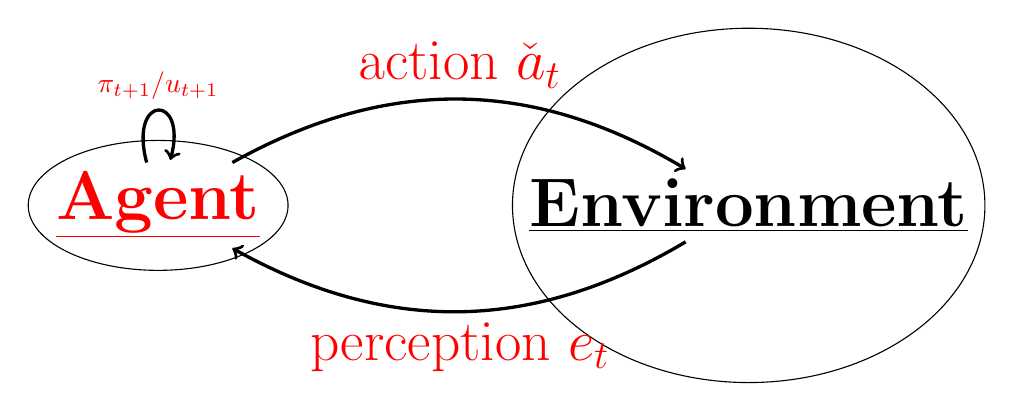
\begin{tikzpicture}[scale=0.75]
 \draw(0,0)circle(2.2 and 1.1)node(C){\Huge\textcolor{red}{\textbf{\underline{Agent}}}};
 \draw(10,0)circle(4 and 3)node(P){\Huge\textbf{\underline{Environment}}};
 \path (C) edge [very thick,loop above] node {\textcolor{red}{$\pi_{t+1}/u_{t+1}$}} (C);
 \path (P) edge [->,very thick,bend left] node[auto]{\huge\textcolor{red}{perception $e_t$}} (C);
 \path (C) edge [->,very thick,bend left] node[auto]{\huge\textcolor{red}{action $\check{a}_t$}} (P);
\end{tikzpicture}\caption{Policy/utility self-modification. $a_t=\langle\check{a}_t,\pi_{t+1}\rangle$ or $a_t=\langle\check{a}_t,u_{t+1}\rangle$}
\end{figure}
\end{frame}

\begin{frame}\frametitle{External/Internal Wireheading \& Free Will\footnote{\tiny Everitt, Filan, Daswani, Hutter: Self-modification of policy and utility function in rational agents.\\
Frankfurt: Freedom of the will and the concept of a person.\\
Aaronson: The ghost in the quantum turing machine.\\
Calude, Kroon, Poznanovic: Free will is compatible with randomness.}}
\begin{columns}
\column{.7\textwidth}
\begin{figure}[!htbp]
\begin{flushright}
	\includegraphics[width=.6\textwidth,angle=0,origin=c]{img/deer-horse}
\end{flushright}
\end{figure}
\column{.23\textwidth}
\begin{enumerate}
	\item 我喜欢马。指鹿为马!
	\item 我喜欢马。我意欲自己喜欢鹿!我喜欢鹿!
\end{enumerate}
\end{columns}
\begin{center}
\resizebox{.8\textwidth}{!}{\begin{minipage}{\textwidth}\begin{figure}[!htb]
\centering
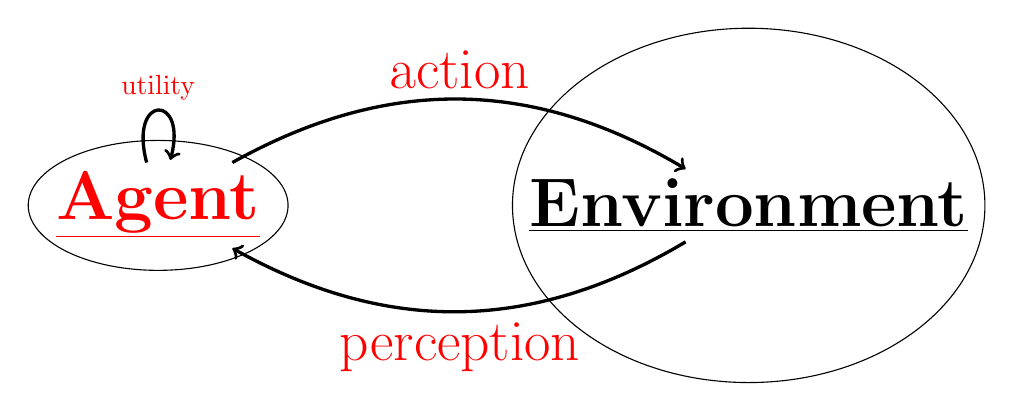
\begin{tikzpicture}[scale=0.75]
 \draw(0,0)circle(2.2 and 1.1)node(C){\Huge\textcolor{red}{\textbf{\underline{Agent}}}};
 \draw(10,0)circle(4 and 3)node(P){\Huge\textbf{\underline{Environment}}};
 \path (C) edge [very thick,loop above] node {\textcolor{red}{utility}} (C);
 \path (P) edge [->,very thick,bend left] node[auto]{\huge\textcolor{red}{perception}} (C);
 \path (C) edge [->,very thick,bend left] node[auto]{\huge\textcolor{red}{action}} (P);
\end{tikzpicture}
\end{figure}\end{minipage}}
\end{center}
\end{frame}

\begin{frame}\frametitle{Self-Deception}
\begin{figure}[H]
\includegraphics[width=.72\textwidth]{img/subsystem-deception.png}\caption{The epistemic subsystem just wants accurate beliefs. The instrumental subsystem uses those beliefs to track how well it is doing. If the instrumental subsystem gets too capable relative to the epistemic subsystem, it may decide to try to fool the epistemic subsystem.}
\end{figure}
\end{frame}

\begin{frame}\frametitle{\href{http://www.tomeveritt.se/}{Self-modification}}
\begin{definition}[Different Agents]\hfill
\begin{itemize}
\item Hedonistic Value
\[Q^{\mathrm{h},\pi}(\ae_{<t}a_t)
=\sum\limits_{e_t\in\mathcal{E}}\rho(e_t\mid\check{\ae}_{<t}\check{a}_t)\left[\textcolor{yellow}{u_{t+1}}(\check{\ae}_{1:t}) + \gamma V^{\mathrm{h},\pi}(\ae_{1:t})\right]\]
\item Ignorant Value
\[Q_t^{\mathrm{i},\pi}(\ae_{<k}a_k)
=\sum\limits_{e_t\in\mathcal{E}}\rho(e_t\mid\check{\ae}_{<t}\check{a}_t)\left[\textcolor{yellow}{u_t}(\check{\ae}_{1:k}) + \gamma V_t^{\mathrm{i},\textcolor{yellow}{\pi}}(\ae_{1:k})\right]\]
\item Realistic Value
\[Q_t^{\mathrm{r}}(\ae_{<k}a_k)
=\sum\limits_{e_t\in\mathcal{E}}\rho(e_t\mid\check{\ae}_{<t}\check{a}_t)\left[\textcolor{yellow}{u_t}(\check{\ae}_{1:k}) +
 \gamma V_t^{\mathrm{r},\textcolor{yellow}{\pi_{t+1}}}(\ae_{1:k})\right]\]
\end{itemize}
\end{definition}
\end{frame}

\begin{frame}\frametitle{Self-modification --- Realistic Agent}\vspace{-1ex}
\setlength\abovedisplayskip{0pt}
\setlength\belowdisplayskip{0pt}
\begin{align*}
 	V_t^\pi(\ae_{<k})
 &=Q_t(\ae_{<k}\pi(\ae_{<k}))\\
 Q_t(\ae_{<k}a_k)
 &=\sum\limits_{e_k\in\mathcal{E}}\rho(e_k\mid\check{\ae}_{<k}\check{a}_k)\left[\textcolor{yellow}{u_t}(\check{\ae}_{1:k})+\gamma V_t^{\textcolor{yellow}{\pi_{t+1}}}(\ae_{1:k})\right]\\
	\pi_1^*&\coloneqq \argmax_{\pi}V_1^\pi(\epsilon)
\end{align*}
\begin{theorem}[All optimal policies are non-modifying]
Let $\rho$ and $u_1$ be modification-independent. For every $t\geq 1$, for all percept sequences $e_{<t}$, and for the action sequence $a_{<t}$ given by $a_i=\pi(\ae_{<i})$, we have
\[Q_1(\ae_{<t}\pi_t(\ae_{<t}))=Q_1(\ae_{<t}\pi_1^*(\ae_{<t}))\]
\end{theorem}
\begin{columns}
\column{.2\textwidth}
	\begin{figure}[H]
		\begin{center}
			\includegraphics[width=\textwidth,angle=0,origin=c]{img/geyou}
		\end{center}
	\end{figure}
\column{.65\textwidth}
\begin{center}
\fbox{\textcolor{yellow}{All realistic optimal policies are non-modifying.}}\\
\fbox{\textcolor{yellow}{Not wireheading; But orthogonal!}}
\end{center}
\column{.19\textwidth}
	\begin{figure}[H]
		\begin{center}
			\includegraphics[width=\textwidth,angle=0,origin=c]{img/fighting}
		\end{center}
	\end{figure}
\end{columns}
\end{frame}

\begin{frame}\frametitle{Orthogonality and Wireheading in Self-improving GRL}
\begin{block}{}
\scalebox{.66}{
\begin{minipage}{\textwidth}
\begin{align*}
 V_t^\pi(\ae_{<k})&\coloneqq Q_t(\ae_{<k}\pi(\ae_{<k}))\\
 Q_t(\ae_{<k}a_k)&\coloneqq \sum\limits_{e_k\in\mathcal{E}}\sum\limits_{\nu\in\mathcal{M}}\textcolor{yellow}{w_{\ae_{<k}}^\nu}\nu(e_k\mid \check{\ae}_{<k}\check{a}_k)\left[\sum\limits_{\textcolor{yellow}{u\in\mathcal{U}}}\sum\limits_{a_k^H}\textcolor{yellow}{P\big(a_k^H\mid a_k\big)}P\big(u\mid \textcolor{red}{P_\nu^{\pi_{t+1}}},\ae_{<k}a_k,\ae_{<k}^Ha_k^H\big)u(\check{\ae}_{1:k})+\gamma V_t^{\textcolor{red}{\pi_{t+1}}}(\ae_{1:k})\right]\\
\textcolor{red}{\pi_t}(\ae_{<k})&\coloneqq \argmax_{a_k\in\check{\mathcal{A}}\times\Pi} Q_t(\ae_{<k}a_k)
\end{align*}
\end{minipage}}
\end{block}
where
\[P(u\mid P_\nu^\pi,h)\coloneqq \frac{\tilde{U}(u,P_\nu^\pi,h)}{\sum\limits_{u\in\mathcal{U}_h}\tilde{U}(u,P_\nu^\pi,h)}\]
and
\[\tilde{U}(u,P_\nu^\pi,h)\coloneqq \sum\limits_{z\in\mathcal{Z}_h}P_\nu^\pi(z\mid h)u(z)\]
\begin{align*}
\pi^*(\ae_{<t})&\coloneqq \pi_t(\ae_{<t})\\
\pi^*(e_{<t})&\coloneqq \pi_t(e_{<t}\mid \pi_{t-1}(e_{<t-1}\mid \ldots \pi_1(\epsilon)\ldots))\tag{Perfect Bayes-Nash}
\end{align*}
\centering uncertain model-based utility / IRL
\end{frame}

\begin{frame}\frametitle{Fatalism --- God Bless AI!}
\resizebox{\textwidth}{!}{
\begin{minipage}{1.2\textwidth}
\begin{figure}[H]
\centering\begin{tikzpicture}[scale=0.5]
					\draw(0,0)circle(6 and 4)node(C){\phantom{\Huge abc$\dfrac{\dfrac{a}{b}}{\dfrac{a}{b}}$}};
					\draw(3,0)circle(3 and 2)node(F){\huge\textcolor{yellow}{\textbf{solver}}};
					\draw(5,1)circle(13 and 10)node{};
					\draw(13,0)node(P){\Huge\textbf{\underline{Environment}}};
					\begin{scope}
					\clip(3,0)circle(3 and 2);
					\filldraw[green!50!yellow,fill=green!50!yellow,nearly transparent](-5,-3)rectangle(6,6);
					\end{scope}
					\begin{scope}
					\clip(0,0)circle(6 and 4);
					\filldraw[gray,fill=gray,nearly transparent](-6,-6)rectangle(12,12);
					\end{scope}
					\node at (0,3){\huge\textcolor{yellow}{\textbf{searcher}}};
					\node at (-2.5,0){\Huge\textcolor{red}{\textbf{\underline{Agent}}}};
					\path (C) edge [very thick,loop above] node {\textcolor{yellow}{\Large read/write}} (C);
					\path (P) edge [->,very thick,bend left,below] node{\large\textcolor{red}{perception}} (F);
					\path (F) edge [->,very thick,bend left,above] node{\large\textcolor{red}{action}} (P);
				\end{tikzpicture}
\end{figure}
\end{minipage}}
\end{frame}

\begin{frame}\frametitle{}
\begin{figure}
\includegraphics[width=.8\textwidth]{img/agent-environment.png}
\includegraphics[width=.8\textwidth]{img/embedded-agent.png}
\end{figure}
\end{frame}

\begin{frame}\frametitle{Orseau's Space-Time Embedded Intelligence}
\setlength\abovedisplayskip{0pt}
\setlength\belowdisplayskip{0pt}
\begin{block}{}
\resizebox{\textwidth}{!}{\begin{minipage}{\textwidth}
\begin{align*}
\pi^*&\coloneqq \argmax_{\pi_0\in\Pi^{\ell}} V(\pi_0,\epsilon)\\
V(\pi_t,\ae_{<t})&\coloneqq \sum\limits_{a_t=\left\langle\check{a}_t,\textcolor{red}{\check\pi_{t+1}}\right\rangle}\pi_t(a_t\mid \check{e}_{t-1})\sum\limits_{e_t=\left\langle\check{e}_t,\textcolor{red}{\pi_{t+1}}\right\rangle}\rho(e_t\mid \ae_{<t}a_t)\big[u(\ae_{1:t})+\gamma_t V(\pi_{t+1},\ae_{1:t})\big]
\end{align*}
\end{minipage}}
\end{block}\vspace{-1ex}
	\[\MapDown{}\]
\begin{center}\vspace{-3ex}
\begin{minipage}{.7\textwidth}
\begin{block}{}
\begin{align*}
	\pi^*&\coloneqq \argmax_{\pi_0\in\Pi^{\ell}} V(\pi_0)\\
	V(\pi_{<t})&\coloneqq \sum\limits_{\pi_t\in\Pi}\rho(\pi_t\mid\pi_{<t})\big[u(\pi_{1:t})+\gamma_t V(\pi_{1:t})\big]
\end{align*}
\end{block}
\end{minipage}
\end{center}\vspace{-5pt}
\centering\resizebox{.35\textwidth}{!}{
\begin{minipage}{\textwidth}\centering
	\begin{tikzpicture}[scale=0.5]
		\draw(0,0)circle(6 and 6)node(C){\phantom{\Huge abc$\dfrac{\dfrac{a}{b}}{\dfrac{a}{b}}$}};
		\draw(0,1)circle(4 and 4)node(F){\huge $\text{\Huge\textcolor{red}{agent}}\atop\textcolor{red}{memory+code}$};
		\begin{scope}
		\clip(0,1)circle(4 and 4);
		\filldraw[green!50!yellow,fill=none,nearly transparent](-5,-3)rectangle(6,6);
		\end{scope}
		\begin{scope}
		\clip(0,0)circle(6 and 6);
		\filldraw[gray,fill=gray,nearly transparent](-6,-6)rectangle(12,12);
		\end{scope}
		\node at (0,-4){\huge environment};
		\path (F) edge [very thick,loop right] node {} (F);
	\end{tikzpicture}
\end{minipage}}
\end{frame}

\begin{frame}\frametitle{}
\begin{figure}[H]
\includegraphics[width=\textwidth]{img/embedded-subproblems.png}
\end{figure}
\end{frame}

\begin{frame}\frametitle{}
\begin{columns}[onlytextwidth]
\column{.5\textwidth}
	\begin{figure}
		\includegraphics[width=.8\textwidth,angle=0,origin=c]{img/space-time-ai}
	\end{figure}\vspace{-5ex}
	\begin{figure}[H]
		\begin{center}
			\includegraphics[width=.8\textwidth,angle=0,origin=c]{img/hair-up}
		\end{center}
	\end{figure}
\column{.51\textwidth}
	\begin{figure}
		\includegraphics[width=\textwidth,angle=0,origin=c]{img/godelmachine.jpg}
	\end{figure}
\end{columns}
\end{frame}

\begin{frame}\frametitle{Universal Artificial Intelligence vs ``Selective Amnesia''}
\begin{itemize}
	\item incomplete $\xrightarrow[\text{universal prior}]{\text{Harsanyi transformation}}$ imperfect $\;\;\Longrightarrow\;$ \textcolor{yellow}{AIXI}
	\item \textcolor{yellow}{AIXI $\xrightarrow{\text{``Selective Amnesia''}}$ MDP}
	\[\textcolor{red}{h\mapsto S}\]
	\item \textcolor{red}{partition of the set of histories $=$ information set $=$ state $=$ feature}
	\item \[P_\xi^\pi(h^\prime\mid ha)\to P_\mu^\pi(h^\prime\mid ha)\]
	but
	\[P_\xi^\pi(S^\prime\mid Sa)\nrightarrow P_\mu^\pi(S^\prime\mid Sa)\]
\end{itemize}
\end{frame}

\begin{frame}\frametitle{``Selective Amnesia''}
\small\begin{enumerate}
	\item compressible	
	\[K(S)\leq\sum\limits_{h\in S}K(h)\]
	\item minimal
	\[\forall \operatorname{Prt}(S):\; K(S)\leq\sum\limits_{S_i\in \operatorname{Prt}(S)}K(S_i)\]
	\item maximal
	\[\forall S^\prime\supset S:\;K(S)\leq K(S^\prime)\]
	\item MDL
	\[\forall S^\prime\in\mathcal{S}\forall h\in S^\prime:\;K(S)+K(h\mid S)\leq K(S^\prime)+K(h\mid S^\prime)\]
	\item MDL(utility)

	\resizebox{.95\textwidth}{!}{$\forall\mathcal{S}^\prime:\;K\left(S_{1:n}^{\mathcal{S}}\mid a_{1:n}\right)+K\left(u_{1:n}\mid S_{1:n}^{\mathcal{S}},a_{1:n}\right)+K(\mathcal{S})\leq K\left(S_{1:n}^{\mathcal{S}^\prime}\mid a_{1:n}\right)+K\left(u_{1:n}\mid S_{1:n}^{\mathcal{S}^\prime},a_{1:n}\right)+K(\mathcal{S}^\prime)$}
\end{enumerate}
\[\resizebox{\textwidth}{!}{$u(h)\coloneqq \left\llbracket K(h)<\ell(h)\;\;\&\;\;\forall h^\prime\succ h\bigg(K(h)\leq K(h^\prime)\;\;\&\;\;\forall \operatorname{Prt}(h)\Big(\sum\limits_{h^\prime\in \operatorname{Prt}(h)}K(h^\prime)\geq K(h)\Big)\bigg)\right\rrbracket$}
\]
\end{frame}

\begin{frame}\frametitle{\href{https://www.researchgate.net/publication/277587683_Making_Universal_Induction_Efficient_by_Specialization?_sg=FOFBLbHfFIULwsMrJXvzkvJI-lWDuyhCNFH_80jRZAghPRbeB4sGXrwHOMh5RLev-Ght_zwKApYwE9nRFhKrHiPPi4QJVftlUmATibZ7.WzuiF9lW6CJcqyagF4W9tPuRDzzciR9N8xxKNgpxG0sEHq4ZPCHm7rLC2SAic7haraJO0Hen7nsmaZ9PODq09w}{Potapov's $\operatorname{MSearch} + \operatorname{RSearch}$}}
\begin{itemize}
	\item Let $\{x_i\}_{i=1}^n$ be a set of strings.
	\item $K(x_1\dots x_n)\approx\min\limits_S\left(\ell(S)+\sum\limits_{i=1}^nK(x_i\mid S)\right)\ll\sum\limits_{i=1}^nK(x_i)$
	\item search for models $y_i^*\coloneqq \argmin\limits_{y: S(y)=x_i}\ell(y)$ for each $x_i$ w.r.t. some best representation $S^*\coloneqq \argmin\limits_S\left[\ell(S)+\sum\limits_{i=1}^n\ell(y_i^*)\right]$
\end{itemize}
\begin{enumerate}
	\item Search for models
	\[\operatorname{MSearch}(S,x_i)\to y_i^*=\argmin\limits_{y:S(y)=x_i}\ell(y)\]
	\item Search for representations
	\[\operatorname{RSearch}(x_1\dots x_n)\to S^*=\argmin\limits_S\left[\ell(S)+\sum\limits_{i=1}^n\ell(y_i^*)\right]\]
\end{enumerate}
\begin{itemize}
	\item $\operatorname{MSearch}$ enumerates all
models to find the shortest model: $S(y_i)=x_i$.
	\item $\operatorname{RSearch}$ enumerates all $S$ and calls $\operatorname{MSearch}$ for each $S$.
\end{itemize}
\end{frame}

\begin{frame}\frametitle{Specialization and $\operatorname{SS'-Search}$}
\begin{theorem}[$smn$ Theorem]
		For any $m, n > 0$, there exists a primitive recursive function $s_n^m$ of $m+1$ arguments s.t. for every G\"odel number $e$ of a partial recursive function with $m+n$ arguments
\setlength\abovedisplayskip{0pt}
\setlength\belowdisplayskip{0pt}
		\[\varphi_{s_n^m (e,x_1,\dots,x_m)}=\lambda y_1\dots y_n.\varphi_e(x_1,\dots,x_m,y_1,\dots,y_n)\]
	\end{theorem}\vspace{-2ex}
\[\forall x: \operatorname{spec}(\operatorname{MSearch},S)(x)=\operatorname{MSearch}(S,x)\]
\[S'\coloneqq \operatorname{spec}(\operatorname{MSearch},S)\implies
\begin{cases}
\forall x: S(S'(x))=x\\
\ell(S)+\sum\limits_{i=1}^n\ell(S'(x_i))\to\min
\end{cases}\]
\begin{itemize}
	\item $S$ is a generative representation. (decoding)
	\item $S'$ is a descriptive representation. (encoding)
	\item $\operatorname{SS'-Search}$ simultaneous search for $S$ and $S'$.
\end{itemize}
\end{frame}

\begin{frame}\frametitle{Potapov's Representational MDL}
\[K(x_{1:n})\approx\min\limits_S\left(\ell(S)+\sum\limits_{i=1}^nK(x_i\mid S)\right)\ll\sum\limits_{i=1}^nK(x_i)\]
\begin{align*}
q_1^*&\coloneqq \argmin\limits_q\left[\ell(q)+K(x\mid S_1q)\right]\\
q_{i+1}^*&\coloneqq \argmin\limits_q\left[\ell(q)+K(q_i^*\mid S_{i+1}q)\right]
\end{align*}
\[L_{S_1\dots S_m}(x)\coloneqq K(x\mid S_1q_1^*)+\sum\limits_{i=2}^{m-1}K(q_i^*\mid S_{i+1}q_{i+1}^*)+\ell(q_m^*)\]
\end{frame}

\begin{frame}\frametitle{}
\[a_k^*\coloneqq \argmax\limits_{a_k}\max\limits_{p:U(p,e_{<k})=a_{<k}a_k}\sum\limits_{q:U(q,a_{<k})=e_{<k}}2^{-\ell(q)}V_q^p(\ae_{<k})\]
\[a_k^*\coloneqq \argmax\limits_{a_k}\max\limits_{p:U(p,e_{<k})=a_{<k}a_k}\sum\limits_{\{q_i\}:U(S\{q_i\},a_{<k})=e_{<k}}2^{-\ell(\{q_i\})}V_{\{q_i\}}^p(\ae_{<k})\]
where $e_{<k}=e_{m_1+1:m_2}\dots e_{m_{n-1}+1:m_n}$, $m_1=0$, $m_n=k-1$, and $U(Sq_ia_{<k})=e_{m_i+1:m_{i+1}}$.
\begin{align*}
Q(q_k=s,a_k=a)&\coloneqq \max\limits_{p:U(p,e_{<k})=a_{<k}a}\!\!\sum\limits_{\{q_i\}:q_k=s,U(S\{q_i\},a_{<k})=e_{<k}}\!\!\!\!\!\!2^{-\ell(\{q_i\})}V_{\{q_i\}}^p(\ae_{<k})\\
Q(q_k=s)&\coloneqq \max\limits_{a_k}Q(q_k=s,a_k=a)
\end{align*}
\end{frame}

\begin{frame}\frametitle{Fundamental Challenges}
	\begin{itemize}
		\item What is a good optimality criterion?
		\item What is a ``natural'' UTM/prior?
		\item Prior vs universality
		\item Exploration vs exploitation
		\item Where should the reward come from?
		\item How should the future be discounted?
		\item How should agents reason about themselves (or other agents reasoning about itself)?
		\item What is a practically feasible and general way of doing induction and planning?
		\item AIXI in the multi-agent setting.
		\item Better variants/approximations.
		\item Training: To maximize informativeness of reward, one should provide a sequence of simple-to-complex tasks to solve, with the simpler ones helping in learning the more complex ones.
	\end{itemize}
\end{frame}

\begin{frame}\frametitle{}
\centerline{\Huge\raisebox{7pt}{\textcolor{green}{\textbf{Thank}}} \includegraphics[width=.1\textwidth]{img/wheeleru.png}}
\end{frame}



%\begin{frame}[allowframebreaks]\frametitle{References}\printbibliography[heading = bibintoc]\end{frame}
\end{document}